% ============================================================
% Qiushi Writing — English Book Template
% Goal: clean, stable, book-like PDF output for technical and general books.
% Compile: latexmk -lualatex -interaction=nonstopmode main.tex
% If LuaLaTeX cache is not writable, run:
%   TEXMFVAR=/tmp/qiushi_texmf_var latexmk -lualatex -interaction=nonstopmode main.tex
% ============================================================
\documentclass[11pt,a4paper,openany]{book}
\providecommand{\BookTemplateVersion}{2026.04.30}

% ── Book Metadata ────────────────────────────────────────────
\newcommand{\BookTitle}{Non-Hermitian Photonics}
\newcommand{\BookSubtitle}{Maxwell Operators, Open Resonances, and Topological Light}
\newcommand{\BookAuthorPlain}{Wenhao Li and Yihao Yang}
\newcommand{\BookAuthor}{Wenhao Li and Yihao Yang\textsuperscript{*}}
\newcommand{\BookCorrespondingAuthor}{\textsuperscript{*}Corresponding author: \href{mailto:yangyihao@zju.edu.cn}{yangyihao@zju.edu.cn}}
\newcommand{\BookPublisher}{Qiushi Writing}
\newcommand{\BookEdition}{First Edition}
\newcommand{\BookDate}{\today}
\newcommand{\BookDescription}{%
A monograph on the spectral, scattering, modal, and topological theory
of Maxwell equations when material response, radiation boundary conditions,
gain, loss, dispersion, and openness destroy the ordinary self-adjoint structure
of closed lossless electromagnetism.  Starting from Maxwell's equations and
classical optics, the book develops the physical origins of non-Hermiticity
in photonic systems, the theory of quasinormal modes, exceptional points,
$\mathcal{PT}$-symmetric optics, non-Hermitian band topology, the skin effect,
and bound states in the continuum, with applications to lasers, absorbers,
sensors, and topological devices.}

% ── Core Math and Units ─────────────────────────────────────
\usepackage{amsmath,amssymb,amsthm,mathtools}
\usepackage{bm}
\usepackage{siunitx}
\sisetup{detect-all=true,per-mode=symbol}

% Minimal physics-style helpers.
\newcommand{\dd}{\mathop{}\!\mathrm{d}}
\newcommand{\dv}[2]{\frac{\dd #1}{\dd #2}}
\newcommand{\pdv}[2]{\frac{\partial #1}{\partial #2}}
\newcommand{\ket}[1]{\left|#1\right\rangle}
\newcommand{\bra}[1]{\left\langle#1\right|}
\newcommand{\braket}[2]{\left\langle#1\,\middle|\,#2\right\rangle}

% ── Graphics and Diagrams ───────────────────────────────────
\usepackage{graphicx}
\usepackage[dvipsnames]{xcolor}
\usepackage{tikz}
\usepackage{pgfplots}
\pgfplotsset{compat=1.18}
\graphicspath{{figures/}{../../workspace/figures/}}

% ── Bibliography guard ──────────────────────────────────────
\newif\ifQiushiHasCitations
\let\QiushiOriginalCite\cite
\renewcommand{\cite}{\global\QiushiHasCitationstrue\QiushiOriginalCite}
\let\QiushiOriginalNocite\nocite
\renewcommand{\nocite}{\global\QiushiHasCitationstrue\QiushiOriginalNocite}

% ── Tables ──────────────────────────────────────────────────
\usepackage{booktabs,longtable,array,tabularx,makecell,multirow}
\renewcommand{\arraystretch}{1.16}

% ── Code and Algorithms ─────────────────────────────────────
\usepackage{listings}
\usepackage[ruled,vlined,linesnumbered]{algorithm2e}

% ── Layout and Typography ───────────────────────────────────
\usepackage[
    inner=2.8cm,
    outer=2.25cm,
    top=2.55cm,
    bottom=2.75cm,
    headheight=23pt,
    headsep=0.75cm,
    footskip=1.0cm
]{geometry}
\usepackage{setspace}
\setstretch{1.13}
\setlength{\parindent}{1.25em}
\setlength{\parskip}{0.18em plus 0.08em}
\raggedbottom
\emergencystretch=3em
\clubpenalty=10000
\widowpenalty=10000

\usepackage{microtype}
\usepackage{caption,subcaption}
\usepackage{enumitem}
\setlist{itemsep=0.25em,topsep=0.45em,parsep=0.1em}
\usepackage{float}
\usepackage{needspace}

% ── Calm Book Palette ───────────────────────────────────────
\definecolor{BookBlue}{HTML}{25476A}
\definecolor{BookAccent}{HTML}{8A5A2B}
\definecolor{BookMuted}{HTML}{6F7782}
\definecolor{BookLight}{HTML}{F4F7FA}
\definecolor{BookWarm}{HTML}{FAF7F1}
\definecolor{BookRule}{HTML}{D6DDE5}
\definecolor{CodeBg}{HTML}{F7F7F4}
\definecolor{QiushiBlue}{HTML}{003F88}

% ── Chapter and Section Style ───────────────────────────────
\usepackage{titlesec}
\titleformat{\chapter}[display]
  {\normalfont\bfseries\color{BookBlue}}
  {\Large\color{BookAccent}\chaptername\ \thechapter}
  {0.6em}
  {\Huge}
  [\vspace{0.6em}{\color{BookAccent}\rule{\textwidth}{0.6pt}}]
\titlespacing*{\chapter}{0pt}{2em}{2.1em}
\titleformat{\section}{\Large\bfseries\color{BookBlue}}{\thesection}{0.75em}{}
\titleformat{\subsection}{\large\bfseries\color{black}}{\thesubsection}{0.65em}{}

% ── Headers and Footers ─────────────────────────────────────
\usepackage{fancyhdr}
\pagestyle{fancy}
\fancyhf{}
\fancyhead[LE]{\small\color{BookMuted}\nouppercase{\leftmark}}
\fancyhead[RO]{\small\color{BookMuted}\nouppercase{\rightmark}}
\fancyfoot[L]{}
\fancyfoot[R]{\small\thepage}
\renewcommand{\headrulewidth}{0.4pt}
\renewcommand{\headrule}{\hbox to\headwidth{\color{BookRule}\leaders\hrule height \headrulewidth\hfill}}
\renewcommand{\footrulewidth}{0.4pt}
\renewcommand{\footrule}{\hbox to\headwidth{\color{BookRule}\leaders\hrule height \footrulewidth\hfill}}
\fancypagestyle{plain}{
    \fancyhf{}
    \fancyfoot[L]{}
    \fancyfoot[R]{\small\thepage}
    \renewcommand{\headrulewidth}{0pt}
    \renewcommand{\footrulewidth}{0.4pt}
    \renewcommand{\footrule}{\hbox to\headwidth{\color{BookRule}\leaders\hrule height \footrulewidth\hfill}}
}

% ── Captions, Code, and Useful Boxes ────────────────────────
\captionsetup{
    font=small,
    labelfont={bf,color=BookBlue},
    labelsep=quad,
    skip=0.55em
}
\lstset{
    basicstyle=\ttfamily\small,
    backgroundcolor=\color{CodeBg},
    breaklines=true,
    breakatwhitespace=false,
    breakautoindent=true,
    columns=fullflexible,
    keepspaces=true,
    frame=single,
    rulecolor=\color{BookRule},
    numbers=left,
    numberstyle=\tiny\color{BookMuted},
    keywordstyle=\color{BookBlue}\bfseries,
    commentstyle=\color{BookMuted},
    stringstyle=\color{BookAccent},
    showstringspaces=false,
    tabsize=4
}

\usepackage{tcolorbox}
\tcbuselibrary{breakable}
\newtcolorbox{booknote}[1][Note]{
    breakable,
    colback=BookLight,
    colframe=BookBlue,
    coltitle=white,
    title=\textbf{#1},
    boxrule=0.6pt,
    arc=1mm,
    left=8pt,right=8pt,top=6pt,bottom=6pt
}
\newtcolorbox{takeaway}[1][Takeaway]{
    breakable,
    colback=BookWarm,
    colframe=BookAccent,
    coltitle=white,
    title=\textbf{#1},
    boxrule=0.6pt,
    arc=1mm,
    left=8pt,right=8pt,top=6pt,bottom=6pt
}
\newenvironment{chapterlead}
  {\begin{quote}\large\itshape\color{BookMuted}}
  {\end{quote}\vspace{0.6em}}

% ── Theorem Environments ────────────────────────────────────
\newtheoremstyle{bookplain}
  {0.8em}{0.8em}{\itshape}{}{\bfseries\color{BookBlue}}{.}{0.5em}{}
\newtheoremstyle{bookdefinition}
  {0.8em}{0.8em}{}{}{\bfseries\color{BookBlue}}{.}{0.5em}{}
\theoremstyle{bookplain}
\newtheorem{theorem}{Theorem}[chapter]
\newtheorem{lemma}[theorem]{Lemma}
\newtheorem{proposition}[theorem]{Proposition}
\newtheorem{corollary}[theorem]{Corollary}
\theoremstyle{bookdefinition}
\newtheorem{definition}[theorem]{Definition}
\newtheorem{example}{Example}[chapter]
\theoremstyle{remark}
\newtheorem{remark}{Remark}[chapter]

% ── Links and References ────────────────────────────────────
\usepackage{xurl}
\usepackage{hyperref}
\hypersetup{
    colorlinks=true,
    linkcolor=BookBlue,
    citecolor=BookAccent,
    urlcolor=BookBlue,
    pdfauthor={\BookAuthor},
    pdftitle={\BookTitle}
}
\usepackage{bookmark}
\usepackage{cleveref}

% ── Long paths, URLs, wrapping tables ───────────────────────
\DeclareUrlCommand\qpath{\urlstyle{tt}\small}
\DeclareUrlCommand\qurl{\urlstyle{same}\small}
\DeclareUrlCommand\qcode{\urlstyle{tt}\small}
\Urlmuskip=0mu plus 2mu
\newcolumntype{Y}{>{\raggedright\arraybackslash\hspace{0pt}}X}
\newcolumntype{L}[1]{>{\raggedright\arraybackslash\hspace{0pt}}p{#1}}

% ── Title Page ──────────────────────────────────────────────
\newcommand{\MakeBookTitle}{
\begin{titlepage}
\centering
\vspace*{1.2cm}
{\color{BookAccent}\rule{\textwidth}{1.1pt}}\par
\vspace{2.0cm}
{\Huge\bfseries\color{BookBlue}\BookTitle\par}
\vspace{0.65cm}
{\Large\color{BookMuted}\BookSubtitle\par}
\vspace{1.7cm}
{\Large\BookAuthor\par}
\vspace{0.35cm}
{\small\color{BookMuted}\BookCorrespondingAuthor\par}
\vspace{0.45cm}
{\normalsize\BookEdition\par}
\vfill
\begin{minipage}{0.78\textwidth}
\centering
\small\color{BookMuted}\BookDescription
\end{minipage}
\vfill
{\small \BookPublisher\quad|\quad \BookDate\par}
\vspace{0.7cm}
{\color{BookAccent}\rule{0.55\textwidth}{0.8pt}}\par
\end{titlepage}
}

% ── Project-level macros ────────────────────────────────────
\IfFileExists{macros.tex}{% ── Non-Hermitian Photonics — Project Macros ────────────────
% Domain-specific commands used throughout the monograph.
% Keep this file lean; add only macros used in multiple chapters.

% ── Maxwell fields and operators ────────────────────────────
\newcommand{\EE}{\mathbf{E}}             % electric field
\newcommand{\HH}{\mathbf{H}}             % magnetic field
\newcommand{\BB}{\mathbf{B}}             % magnetic flux density
\newcommand{\DD}{\mathbf{D}}             % displacement field
\newcommand{\JJ}{\mathbf{J}}             % current density
\newcommand{\FF}{\mathbf{F}}             % generic vector field
\renewcommand{\SS}{\mathbf{S}}           % Poynting vector or generic vector
\newcommand{\rr}{\mathbf{r}}             % position vector
\renewcommand{\aa}{\mathbf{a}}           % lattice vector
\newcommand{\kk}{\mathbf{k}}             % wave vector
\newcommand{\GG}{\mathbf{G}}             % reciprocal lattice vector
\newcommand{\nn}{\hat{\mathbf{n}}}       % unit normal
\newcommand{\curl}{\nabla\times}         % curl operator
\newcommand{\divg}{\nabla\cdot}          % divergence
\newcommand{\grad}{\nabla}               % gradient

% ── Permittivity and permeability ───────────────────────────
\newcommand{\eps}{\varepsilon}            % permittivity
\newcommand{\epsr}{\varepsilon_{\mathrm{r}}}  % relative permittivity
\newcommand{\mur}{\mu_{\mathrm{r}}}      % relative permeability
\newcommand{\epsc}{\tilde{\varepsilon}}   % complex permittivity (with tilde)

% ── Operators ───────────────────────────────────────────────
\newcommand{\Lop}{\hat{\mathcal{L}}}     % generic linear operator
\newcommand{\Mop}{\hat{\Theta}}          % Maxwell curl-curl operator
\newcommand{\adj}{\dagger}               % Hermitian adjoint
\newcommand{\transpose}{\mathsf{T}}      % transpose
\DeclareMathOperator{\tr}{tr}             % trace
\DeclareMathOperator{\diag}{diag}         % diagonal matrix
\DeclareMathOperator{\Res}{Res}           % residue
\renewcommand{\Im}{\operatorname{Im}}      % imaginary part
\renewcommand{\Re}{\operatorname{Re}}      % real part
\DeclareMathOperator{\sgn}{sgn}           % sign function

% ── Non-Hermitian specific ──────────────────────────────────
\newcommand{\PT}{\mathcal{PT}}            % PT symmetry
\newcommand{\Smat}{\mathbf{S}}           % scattering matrix
\newcommand{\Tmat}{\mathbf{T}}           % transfer matrix
\newcommand{\omtil}{\tilde{\omega}}       % complex frequency
\newcommand{\GBZ}{\mathrm{GBZ}}          % generalized Brillouin zone
\newcommand{\BZ}{\mathrm{BZ}}            % Brillouin zone
\newcommand{\NHSE}{\mathrm{NHSE}}        % non-Hermitian skin effect
\newcommand{\wnum}{W}                     % winding number
\newcommand{\Chern}{\mathcal{C}}          % Chern number

% ── Berry phase and topology ────────────────────────────────
\newcommand{\Acal}{\mathcal{A}}           % Berry connection
\newcommand{\Fcal}{\mathcal{F}}           % Berry curvature
\newcommand{\Qfac}{Q}                     % quality factor

% ── Biorthogonal inner product ──────────────────────────────
\newcommand{\bket}[1]{\left|#1\right\rangle}           % right eigenvector
\newcommand{\bbra}[1]{\left\langle\!\left\langle#1\right|\right.}  % left eigenvector (double angle)
\newcommand{\biinner}[2]{\left\langle\!\left\langle #1 \,\middle|\, #2 \right\rangle\!\right\rangle}  % biorthogonal inner product

% ── Commonly used abbreviations in math ─────────────────────
\newcommand{\cc}{\mathrm{c.c.}}          % complex conjugate
\newcommand{\hc}{\mathrm{h.c.}}          % Hermitian conjugate
\newcommand{\etal}{\textit{et~al.}}       % et al. in text

% ── Units and constants ─────────────────────────────────────
\newcommand{\vac}{0}                      % vacuum subscript
\newcommand{\epsvac}{\varepsilon_0}       % vacuum permittivity
\newcommand{\muvac}{\mu_0}               % vacuum permeability
\newcommand{\cvac}{c}                     % speed of light in vacuum
}{}

% ============================================================
\begin{document}

\frontmatter
\MakeBookTitle
\tableofcontents

\mainmatter

% ════════════════════════════════════════════════════════════
% PART I — Maxwell Equations Become Spectral Theory
% ════════════════════════════════════════════════════════════
\part{Maxwell Equations Become Spectral Theory}

\chapter{Light as an Eigenvalue Problem}
\label{ch:light-eigenvalue}

\begin{chapterlead}
What does it mean to say that light has ``modes''? Every physicist who has
worked with optical cavities, waveguides, or photonic crystals eventually
invokes a set of modes---discrete field patterns, each oscillating at a
single frequency. This chapter shows where those modes come from:
they are eigenvalues and eigenvectors of an operator built from
Maxwell's equations and the material response of the medium.
The structure of that operator---whether it is self-adjoint or not---controls
everything that follows in this book. We shall derive the eigenvalue
problem carefully, explain why it takes the form it does, explore its
mathematical structure through a variational principle, and illustrate it
with a worked one-dimensional example before giving a preview of what
happens when the operator loses its self-adjoint character.Ha hahahahahaahahahah.aaaaaaaaaaaaaabbbbbbbbbbbbbbbbbbbb
\end{chapterlead}


%% ================================================================
\section{Maxwell's equations in matter}
\label{sec:maxwell-matter}

We begin with the macroscopic Maxwell equations in a linear, time-invariant
medium with no free charges or currents:
\begin{align}
 Hahahahahahah.aaaaaaaaaaaaaaaabbbbbbbbbbbbbbbbbbbbbb \curl \EE(\rr,t) &= -\pdv{\BB(\rr,t)}{t}, \label{eq:faraday}\\[4pt]
 \curl \HH(\rr,t) &= \phantom{-}\pdv{\DD(\rr,t)}{t}, \label{eq:ampere}\\[4pt]
 \divg \DD(\rr,t) &= 0, \label{eq:gauss-e}\\[4pt]
 \divg \BB(\rr,t) &= 0. \label{eq:gauss-m}
\end{align}
These four equations, supplemented by constitutive relations connecting
$\DD$ to $\EE$ and $\BB$ to $\HH$, form the complete classical description of
electromagnetic fields in matter. Nothing in this book requires quantum
electrodynamics; the entire non-Hermitian structure we shall develop is
already present at the level of classical Maxwell theory.

In the simplest case the constitutive relations are local and instantaneous:
\begin{equation}
 \DD(\rr,t) = \epsvac\,\epsr(\rr)\,\EE(\rr,t),
 \qquad
 \BB(\rr,t) = \muvac\,\mur(\rr)\,\HH(\rr,t).
 \label{eq:constitutive-simple}
\end{equation}
Here $\epsr(\rr)$ and $\mur(\rr)$ are the relative permittivity and
permeability, which we allow to vary in space but, for now, take to be real
and positive. These assumptions will be progressively relaxed in later
chapters: Chapter~\ref{ch:loss-gain-dispersion} introduces complex and
frequency-dependent $\epsr$, Chapter~\ref{ch:qnm} opens the system to
radiation, and Chapter~\ref{ch:pt-symmetric} considers the special spatial
symmetry of balanced gain and loss.

The constitutive relations~\eqref{eq:constitutive-simple} encode all material
information available to the Maxwell operator. From the standpoint of
the eigenvalue problem we are about to derive, $\epsr(\rr)$ is the central
material input: it controls the spatial pattern of the eigenmodes, the
distribution of eigenfrequencies, and---when it becomes complex---the transition
from Hermitian to non-Hermitian spectral theory.

\begin{booknote}[Why macroscopic Maxwell?]
A monograph on non-Hermitian photonics could, in principle, start from the
microscopic Maxwell equations and derive macroscopic constitutive relations.
We choose to start at the macroscopic level for two reasons. First, the
non-Hermitian phenomena we study---complex eigenfrequencies, exceptional
points, non-reciprocal skin effects---arise already in the macroscopic theory
and do not require a microscopic derivation to be well posed. Second, the
macroscopic framework is what connects directly to photonic-crystal band
computations, scattering-matrix measurements, and device design.
\end{booknote}

\begin{figure}[t]
 \centering
 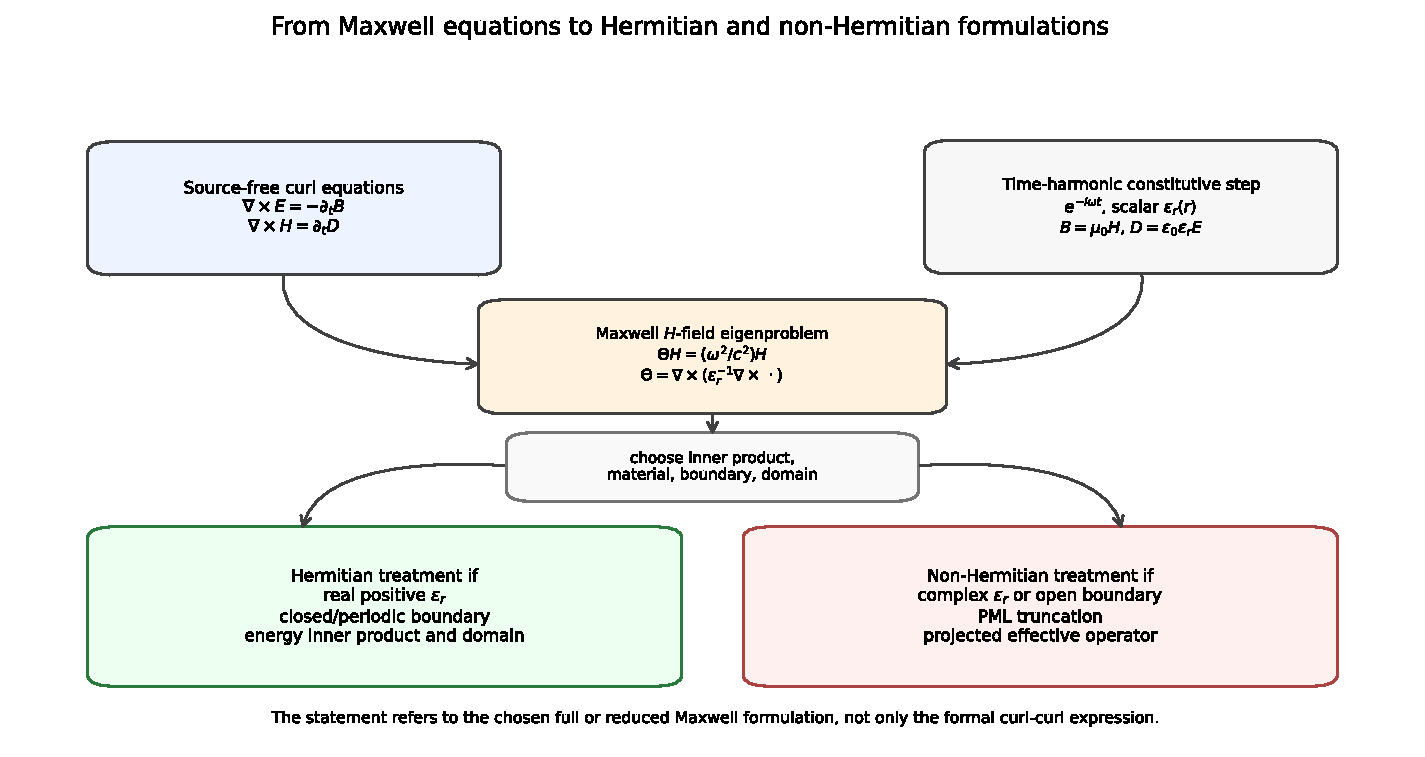
\includegraphics[width=0.98\textwidth]{fig_f1_maxwell_operator_map.pdf}
 \caption{Haahahahahahah.aaaaaaaaaaaaaaaaaabbbbbbbbbbbbbbbbbbb The Maxwell-first route followed in this book. Starting from macroscopic Maxwell equations and constitutive relations, eliminating one field gives the curl--curl operator. When the material is real, the surface term vanishes, and the transverse field space is complete, the operator gives Hermitian photonics. Loss or gain, radiation boundaries, dispersion, and projection onto a subspace lead to the non-Hermitian structures studied in later chapters.}
 \label{fig:maxwell-operator-map}
\end{figure}


%% ================================================================
\section{The frequency-domain eigenproblem hahahahahaaaaaaaaaaaaaabbbbbbbbbbbbbbbbbbbbbb}
\label{sec:freq-domain}

\subsection{Harmonic fields and the time-frequency correspondence}
\label{ssec:harmonic}

For a time-invariant medium it is natural to look for solutions with
harmonic time dependence. We write
\begin{equation}
 \EE(\rr,t) = \Re\!\bigl[\EE(\rr)\,e^{-i\omega t}\bigr],
 \qquad
 \HH(\rr,t) = \Re\!\bigl[\HH(\rr)\,e^{-i\omega t}\bigr],
 \label{eq:harmonic-ansatz}
\end{equation}
where $\omega$ is a real angular frequency and $\EE(\rr)$, $\HH(\rr)$ are
complex-valued spatial amplitudes. At this stage $\omega$ may be regarded
as the real frequency of a harmonic drive. Later, when we solve source-free
open or lossy eigenvalue problems, the same convention will allow
$\omega$ itself to become complex. The sign convention $e^{-i\omega t}$
is standard in the optics and photonics literature; the condensed-matter
convention $e^{+i\omega t}$ leads to conjugated constitutive parameters but
no change in the physics.

The physical content of the harmonic ansatz is that once we know the spatial
amplitude $\EE(\rr)$ at a single frequency $\omega$, we know the complete
space-time field at that frequency. The general time-domain solution is then
recovered by Fourier superposition. The advantage of the frequency-domain
formulation is that the partial differential equations in space-time reduce
to ordinary or partial differential equations in space alone---eigenvalue
problems whose solutions organize the entire electromagnetic response.

\subsection{Deriving the curl--curl eigenproblem}
\label{ssec:curlcurl-derive}

Substituting \eqref{eq:harmonic-ansatz} into Faraday's law
\eqref{eq:faraday} and Amp\`ere's law \eqref{eq:ampere} gives
\begin{align}
 \curl \EE &= i\omega\,\muvac\mur\,\HH, \label{eq:faraday-freq}\\[3pt]
 \curl \HH &= -i\omega\,\epsvac\epsr\,\EE. \label{eq:ampere-freq}
\end{align}
These are two coupled first-order equations for $\EE$ and $\HH$. We can
decouple them by eliminating one field. Applying $\curl$ to
\eqref{eq:ampere-freq} and inserting \eqref{eq:faraday-freq}, we obtain
the \emph{curl--curl eigenproblem for the electric field}:
\begin{equation}
 \boxed{
 \curl\!\left[\frac{1}{\mur(\rr)}\,\curl\EE(\rr)\right]
 = \frac{\omega^2}{c^2}\,\epsr(\rr)\,\EE(\rr).
 }
 \label{eq:curlcurl-E}
\end{equation}
Here $c = 1/\sqrt{\epsvac\muvac}$ is the speed of light in vacuum.
Equation~\eqref{eq:curlcurl-E} is a generalized eigenvalue problem:
the operator on the left acts on $\EE$, the eigenvalue is
$\omega^2/c^2$, and the ``weight'' on the right is the
position-dependent $\epsr(\rr)$.

The elimination procedure is worth understanding in detail, because it
reveals where the operator structure comes from. Writing the two steps
explicitly:
\begin{enumerate}
 \item Use Faraday's law to express the magnetic field as
 $\HH=(i\omega\muvac\mur)^{-1}\curl\EE$.
 \item Insert this expression into Amp\`ere's law:
 \[
 \curl\!\left[\frac{1}{i\omega\muvac\mur}\curl\EE\right]
 = -i\omega\epsvac\epsr\EE,
 \]
 and multiply by $i\omega\muvac$ to obtain
 $\curl[(1/\mur)\curl\EE]=(\omega^2/c^2)\epsr\EE$.
\end{enumerate}
The curl--curl structure on the left is the price we pay for eliminating
one field; the $\epsr$ weight on the right arises from the constitutive
relation. Together they produce a second-order operator in space---directly
analogous to the kinetic-energy operator $-\nabla^2$ in quantum mechanics,
but with the curl replacing the gradient and the permittivity entering as
a generalized eigenvalue weight rather than as an additive potential.

\subsection{The magnetic-field formulation}
\label{ssec:h-formulation}

An analogous equation can be written for $\HH$ alone. Eliminating $\EE$
from \eqref{eq:faraday-freq}--\eqref{eq:ampere-freq} yields
\begin{equation}
 \curl\!\left[\frac{1}{\epsr(\rr)}\,\curl\HH(\rr)\right]
 = \frac{\omega^2}{c^2}\,\mur(\rr)\,\HH(\rr).
 \label{eq:curlcurl-H}
\end{equation}
For non-magnetic media ($\mur = 1$ everywhere), \eqref{eq:curlcurl-H}
simplifies to the standard form used in photonic-crystal theory:
\begin{equation}
 \Mop\,\HH(\rr)
 \;\equiv\;
 \curl\!\left[\frac{1}{\epsr(\rr)}\,\curl\HH(\rr)\right]
 = \frac{\omega^2}{c^2}\,\HH(\rr).
 \label{eq:maxwell-op-H}
\end{equation}
The operator $\Mop$ defined here will be a central object throughout
this book~\cite{figotin2004hamiltonian,raman2010photonic}. Its properties---self-adjointness, compactness of the resolvent,
spectral structure---depend critically on three ingredients:
\begin{enumerate}
 \item the spatial profile of $\epsr(\rr)$ (real or complex, bounded or
 unbounded, periodic or not);
 \item the boundary conditions imposed on $\HH$ at the edges of the
 computational or physical domain;
 \item the function space on which $\Mop$ acts.
\end{enumerate}

Both the $\EE$-field and $\HH$-field formulations are exact restatements
of Maxwell's equations for harmonic fields. However, the $\HH$-field form
has a practical advantage for non-magnetic media: the eigenvalue
$\omega^2/c^2$ appears with a trivial (unit) weight on the right, making
the operator $\Mop$ a standard eigenvalue problem rather than a generalized
one. For this reason, most photonic band-structure codes work with the
$\HH$ formulation, and we shall use $\Mop$ as the default Maxwell operator
throughout this book unless otherwise stated.

\subsection{The divergence constraint}
\label{ssec:divergence}

The curl--curl operator has a large null space: any gradient field
$\HH = \nabla\phi$ satisfies $\curl\HH = 0$ and therefore
$\Mop(\nabla\phi) = 0$. These spurious zero-frequency solutions are
not physical propagating modes; in general they do not satisfy the
transverse constraint $\divg\BB = \muvac\divg\HH = 0$ (or equivalently
$\divg(\epsr\EE) = 0$ in the $\EE$ formulation), and even when a harmonic
gradient field survives as a static zero mode it must be separated from
the dynamical spectrum.

In analytical work, the divergence condition is enforced by restricting
the domain of $\Mop$ to transverse (divergence-free) fields:
\begin{equation}
 \mathcal{H}_{\mathrm{div}} = \bigl\{
 \HH \in L^2(\Omega;\mathbb{C}^3) \;\big|\;
 \divg\HH = 0,\;\text{plus boundary conditions}
 \bigr\}.
 \label{eq:div-free-space}
\end{equation}
On this restricted domain, the null space is eliminated and $\Mop$ becomes
positive semi-definite: all non-static eigenvalues satisfy
$\omega^2/c^2 \ge 0$. This is physically obvious---squared frequencies
cannot be negative in a closed, lossless medium---but mathematically it
relies on the restriction to divergence-free fields and on the treatment
of possible harmonic zero modes.

In numerical work (Chapter~\ref{ch:numerics}), the divergence constraint
must be enforced explicitly, either through a penalty term, a Lagrange
multiplier, or a compatible discretization, such as N\'ed\'elec edge
elements combined with a proper treatment of the gradient null space.
Failure to control this constraint produces spurious modes near
$\omega = 0$ that can contaminate the physical spectrum.


%% ================================================================
\section{Self-adjointness and its physical meaning}
\label{sec:self-adjoint}

\subsection{The electromagnetic inner product}
\label{ssec:em-inner-product}

To ask whether $\Mop$ is self-adjoint, we need an inner product. For
two vector fields $\mathbf{F}$ and $\mathbf{G}$ defined over a domain
$\Omega$, the natural electromagnetic inner product is
\begin{equation}
 \langle \mathbf{F},\,\mathbf{G}\rangle
 \;=\;
 \int_\Omega \mathbf{F}^*(\rr)\cdot\mathbf{G}(\rr)\;\dd^3 r.
 \label{eq:inner-product-plain}
\end{equation}
We also define a weighted inner product:
\begin{equation}
 \langle \mathbf{F},\,\mathbf{G}\rangle_{\eps}
 \;=\;
 \int_\Omega \mathbf{F}^*(\rr)\cdot\epsr(\rr)\,\mathbf{G}(\rr)\;\dd^3 r.
 \label{eq:inner-product}
\end{equation}
Chapter~\ref{ch:energy-inner} develops the physical interpretation of these
inner products in terms of electromagnetic energy.

\subsection{Integration by parts and the boundary term}
\label{ssec:ibp}

We now ask: under what conditions does $\Mop$ satisfy
$\langle\mathbf{F},\,\Mop\mathbf{G}\rangle
 = \langle\Mop\mathbf{F},\,\mathbf{G}\rangle$
for all admissible $\mathbf{F}$ and $\mathbf{G}$? The answer comes
from integration by parts. Using the vector identity
\begin{equation}
 \int_\Omega \mathbf{F}^*\cdot\bigl(\curl\mathbf{A}\bigr)\;\dd^3 r
 =
 \int_\Omega \bigl(\curl\mathbf{F}^*\bigr)\cdot\mathbf{A}\;\dd^3 r
 +
 \oint_{\partial\Omega}
 \bigl(\mathbf{F}^*\times\mathbf{A}\bigr)\cdot\nn\;\dd S,
 \label{eq:curl-ibp}
\end{equation}
applied twice with $\mathbf{A} = (1/\epsr)\curl\mathbf{G}$, one finds
that for $\mur = 1$ the bulk integrals are
symmetric provided $\epsr(\rr)$ is \emph{real}---so that the weight in
\eqref{eq:inner-product} commutes with complex conjugation---and the
surface integral
\begin{equation}
 \oint_{\partial\Omega}
 \left[
 \mathbf{F}^*\times\frac{1}{\epsr}\curl\mathbf{G}
+
 \left(\frac{1}{\epsr}\curl\mathbf{F}\right)^{\!*}\times\mathbf{G}
 \right]\cdot\nn\;\dd S
 = 0
 \label{eq:surface-vanish}
\end{equation}
vanishes. For a closed cavity with perfectly conducting walls
($\nn\times\EE = 0$ on $\partial\Omega$), this surface term is zero. For
a periodic medium with Bloch boundary conditions, it cancels between
opposite faces of the unit cell.

\subsection{The three conditions for Hermitian photonics}
\label{ssec:three-conditions}

\begin{takeaway}[Three conditions for Hermitian photonics]
The Maxwell curl--curl operator $\Mop$ is self-adjoint with respect to
$\langle\cdot,\cdot\rangle$ on divergence-free fields when three conditions
hold simultaneously:
(i)~$\epsr(\rr)$ is real and positive everywhere in $\Omega$
(or, more generally, Hermitian positive definite for anisotropic media);
(ii)~the boundary conditions on $\partial\Omega$ make the surface term
\eqref{eq:surface-vanish} vanish;
(iii)~the domain of $\Mop$ is a complete Hilbert space of transverse
fields, with static null modes removed or treated separately.
Remove any one of these and the spectral theory must be rebuilt.
\end{takeaway}

This result is the foundation on which the entire book rests. Each of the
physical mechanisms that produce non-Hermiticity in photonics can be traced
back to the violation of one of these three conditions:
\begin{itemize}
 \item \textbf{Material loss or gain} (Chapters~\ref{ch:loss-gain-dispersion}
 and~\ref{ch:pt-symmetric}): the permittivity acquires an imaginary part,
 $\epsr \to \epsr' + i\epsr''$, so the weight in
 \eqref{eq:inner-product} is no longer real~\cite{longhi2018parity}. The operator $\Mop$ is
 no longer formally self-adjoint, and its eigenvalues migrate off the
 real axis into the complex plane.
 \item \textbf{Radiation and openness} (Chapters~\ref{ch:boundaries}
 and~\ref{ch:qnm}): outgoing-wave boundary conditions (Sommerfeld
 radiation condition or perfectly matched layers) do not make the surface
 term vanish; instead, energy escapes through $\partial\Omega$. The
 resulting quasinormal modes have complex eigenfrequencies even when
 $\epsr$ is real~\cite{kristensen2011effective,vial2014quasimodal}.
 \item \textbf{Frequency dispersion}
 (Chapter~\ref{ch:loss-gain-dispersion}): when $\epsr$ depends on
 $\omega$, the eigenvalue problem~\eqref{eq:maxwell-op-H} becomes
 nonlinear in the eigenvalue, and the standard spectral theory of
 self-adjoint operators no longer applies directly~\cite{figotin2004hamiltonian}.
 \item \textbf{Projection onto a subspace}
 (Chapter~\ref{ch:maxwell-coupled-modes}): even when the full Maxwell
 operator is self-adjoint, projecting onto a few resonant modes produces
 an effective finite-dimensional Hamiltonian that is generically
 non-Hermitian, because the discarded modes act as an environment~\cite{alpeggiani2017quasinormal}.
\end{itemize}

These four roads to non-Hermiticity are not independent---many real systems
exhibit several simultaneously---but they provide a useful organizational
framework. A $\PT$-symmetric photonic crystal, for example, has
complex $\epsr$ (road~1), may be open to radiation (road~2), may involve
dispersive gain media (road~3), and is often modeled by a few-mode
effective Hamiltonian (road~4).


%% ================================================================
\section{The variational principle}
\label{sec:variational}

Self-adjoint operators with discrete spectra admit a powerful variational
characterization of their eigenvalues. For $\Mop$ on the space of
transverse fields in a closed domain, the Rayleigh quotient is
\begin{equation}
 R[\HH] = \frac{\displaystyle\int_\Omega
 \frac{1}{\epsr(\rr)}\,|\curl\HH(\rr)|^2\;\dd^3 r}
 {\displaystyle\int_\Omega |\HH(\rr)|^2\;\dd^3 r}
 = \frac{\langle\Mop\HH,\,\HH\rangle}{\langle\HH,\,\HH\rangle},
 \label{eq:rayleigh}
\end{equation}
and the fundamental eigenfrequency satisfies the min--max principle:
\begin{equation}
\frac{\omega_1^2}{c^2} = \min_{\HH \in \mathcal{H}_{\mathrm{div}}}
R[\HH].
 \label{eq:minmax}
\end{equation}
where the minimization is over nonzero fields in the dynamical transverse
subspace. Higher eigenfrequencies are obtained by successive minimization
over subspaces orthogonal to the previously found eigenmodes.

The variational principle gives immediate physical insight:
\begin{itemize}
 \item The lowest mode concentrates its magnetic field where
 $1/\epsr$ is smallest, i.e., where the permittivity is largest.
 This is the electromagnetic analogue of a quantum particle
 localizing in a potential well.
 \item Increasing $\epsr$ anywhere in $\Omega$ decreases all
 eigenfrequencies---intuitively, denser media slow light and lower the
 resonant frequencies.
 \item A band gap forms when no trial field can simultaneously satisfy
 the curl constraint and have low energy in a frequency window.
\end{itemize}

The variational principle also explains why the Hermitian eigenfrequencies
are always real: the Rayleigh quotient~\eqref{eq:rayleigh} is manifestly
real when $\epsr$ is real and positive, so $\omega_1^2/c^2$ is real and
non-negative, and $\omega_1$ is real.

\paragraph{What breaks when $\epsr$ is complex.}
If $\epsr$ has an imaginary part, the Rayleigh quotient becomes complex,
and the variational characterization fails: there is no longer a minimum
of a real functional, so the eigenfrequencies are not constrained to the
real axis. This is the variational way of seeing why complex $\epsr$
produces non-Hermitian photonics.


%% ================================================================
\section{Two-dimensional reductions}
\label{sec:2d-reductions}

Many photonic systems---photonic-crystal slabs, ridge waveguides, fiber
cross-sections---have a geometry that is invariant along one spatial
direction. For a system uniform along $z$, all fields can be decomposed
into components with a fixed $z$-dependence $e^{ik_z z}$. At $k_z = 0$
the vector Maxwell equations split into two independent scalar problems,
conventionally called \emph{transverse electric} (TE) and
\emph{transverse magnetic} (TM) polarizations. The common
two-dimensional photonic-crystal convention: TM denotes the scalar
$E_z$ problem and TE denotes the scalar $H_z$ problem. Some waveguide
texts use the opposite language relative to the propagation direction, so
the field component should always be checked.

\subsection{TM polarization}
\label{ssec:tm}

In TM polarization the electric field is parallel to $z$:
$\EE = E_z(\rr_\perp)\,\hat{z}$, where $\rr_\perp = (x,y)$.
The curl--curl equation \eqref{eq:curlcurl-E} reduces to the scalar
Helmholtz equation
\begin{equation}
 -\nabla_\perp\cdot
 \left[\frac{1}{\mur(\rr_\perp)}\,\nabla_\perp E_z(\rr_\perp)\right]
 = \frac{\omega^2}{c^2}\,\epsr(\rr_\perp)\,E_z(\rr_\perp),
 \label{eq:tm-helmholtz}
\end{equation}
where the divergence form is needed if $\mur$ varies in the transverse
plane. For non-magnetic media this simplifies further to
\begin{equation}
 -\nabla_\perp^2 E_z
 = \frac{\omega^2}{c^2}\,\epsr(\rr_\perp)\,E_z.
 \label{eq:tm-simple}
\end{equation}
The eigenvalue is again $\omega^2/c^2$, and the inner product is
\begin{equation}
 \langle f,\,g\rangle_{\eps}^{\mathrm{TM}}
 = \int f^*(x,y)\,\epsr(x,y)\,g(x,y)\;\dd x\,\dd y.
 \label{eq:tm-inner}
\end{equation}

\subsection{TE polarization}
\label{ssec:te}

In TE polarization the magnetic field is parallel to $z$:
$\HH = H_z(\rr_\perp)\,\hat{z}$. The $\HH$-field equation
\eqref{eq:curlcurl-H} reduces to
\begin{equation}
 -\nabla_\perp\cdot
 \left[\frac{1}{\epsr(\rr_\perp)}\,\nabla_\perp H_z(\rr_\perp)\right]
 = \frac{\omega^2}{c^2}\,H_z(\rr_\perp),
 \label{eq:te-helmholtz}
\end{equation}
for $\mur = 1$. The operator on the left is a weighted Laplacian with
$1/\epsr$ as the spatially varying coefficient. The natural TE inner
product is unweighted:
\begin{equation}
 \langle f,\,g\rangle^{\mathrm{TE}}
 = \int f^*(x,y)\,g(x,y)\;\dd x\,\dd y.
 \label{eq:te-inner}
\end{equation}

\begin{remark}
The TE and TM inner products differ because the eigenvalue problem has a
different structure in each polarization. In TM, $\epsr$ appears as a
multiplicative weight on the right-hand side; in TE, $1/\epsr$ appears
inside the differential operator. This asymmetry will become important
when we define Berry curvature (Chapter~\ref{ch:berry-maxwell}) and
biorthogonal products (Chapter~\ref{ch:qnm}) for the two polarizations.
\end{remark}

\subsection{The Schr\"odinger analogy and its limits}
\label{ssec:schrodinger-analogy}

The TM Helmholtz equation~\eqref{eq:tm-simple} bears a striking
resemblance to the time-independent Schr\"odinger equation:
\begin{equation}
 -\frac{\hbar^2}{2m}\nabla^2\psi + V(\rr)\psi = E\psi.
 \label{eq:schrodinger}
\end{equation}
In both cases, a second-order differential operator acts on a scalar
field, and the eigenvalue appears on the right multiplied by a weight.
The analogy is useful for building intuition---photonic band gaps
correspond to electronic band gaps, defect modes correspond to bound
states, and the variational principle operates in both contexts.

However, the analogy has important limits:
\begin{enumerate}
 \item \textbf{Vectorial nature:} Maxwell's equations are inherently
 vectorial. The TE/TM decoupling occurs only in 2D systems at normal
 incidence; in 3D or at oblique incidence, the full vector character of
 the curl--curl operator must be retained.
 \item \textbf{Eigenvalue position:} In Schr\"odinger theory, the
 eigenvalue $E$ appears additively with the potential $V$; in the
 Maxwell problem, $\omega^2/c^2$ appears multiplicatively with $\epsr$.
 This means that the Maxwell spectrum scales homogeneously with the
 dielectric constant, a property that has no Schr\"odinger analogue.
 \item \textbf{No negative eigenvalues:} The Maxwell operator $\Mop$ is
 positive semi-definite on transverse fields, so $\omega^2 \ge 0$ always.
 The Schr\"odinger operator can have negative eigenvalues (bound states
 below the continuum).
 \item \textbf{Non-Hermiticity:} When $\epsr$ is complex, the Maxwell
 eigenvalue problem is \emph{nonlinear} in the eigenvalue if $\epsr$
 depends on $\omega$, while a complex potential in Schr\"odinger theory
 keeps the problem linear. This distinction is important for
 dispersive gain media (Chapter~\ref{ch:loss-gain-dispersion}).
\end{enumerate}


%% ================================================================
\section{Example: one-dimensional photonic crystal}
\label{sec:1d-example}

To make the eigenvalue problem concrete, consider a one-dimensional
periodic dielectric stack: alternating layers of material~A with
permittivity $\varepsilon_A$ and thickness $d_A$, and material~B with
permittivity $\varepsilon_B$ and thickness $d_B$, repeated with period
$a = d_A + d_B$.

\subsection{Bloch modes and the transfer matrix}
\label{ssec:1d-bloch}

By Bloch's theorem (derived in detail in Chapter~\ref{ch:periodicity}),
the eigenmodes of the periodic stack have the form
$E(x) = u_k(x)\,e^{ikx}$, where $u_k(x)$ is periodic with period $a$
and $k$ is the Bloch wave vector restricted to the first Brillouin zone
$[-\pi/a, \pi/a]$.

For a TM-polarized wave propagating along $x$ (the stacking direction),
the problem reduces to a 1D scalar equation. At normal incidence, where
TE and TM have the same dispersion for non-magnetic layers, the standard
approach is the transfer matrix~\cite{raman2010photonic}: across one unit
cell, the field amplitudes $(E, dE/dx)$ are mapped by a $2 \times 2$
matrix $M$ whose trace determines the dispersion relation:
\begin{equation}
 \cos(ka) = \frac{1}{2}\tr M
 = \cos(k_A d_A)\cos(k_B d_B)
 - \frac{1}{2}\left(\frac{n_A}{n_B} + \frac{n_B}{n_A}\right)
 \sin(k_A d_A)\sin(k_B d_B),
 \label{eq:1d-dispersion}
\end{equation}
where $k_j = n_j\omega/c$ and $n_j = \sqrt{\varepsilon_j}$ for
$j \in \{A, B\}$.

\subsection{Band gaps from the eigenvalue perspective}
\label{ssec:1d-gaps}

Equation~\eqref{eq:1d-dispersion} has solutions only when the right-hand
side lies in the interval $[-1, 1]$. When it exceeds this range, there are
no propagating Bloch modes: a \emph{band gap} exists.

From the variational perspective, the band gap arises because no trial
field in the periodic Hilbert space can simultaneously satisfy the curl
(derivative) constraint and the $\epsr$-weighted energy condition in the
gap frequency range. The dielectric contrast $\varepsilon_A/\varepsilon_B$
controls the gap width: larger contrast produces wider gaps.

\paragraph{Numerical illustration.}
Consider $\varepsilon_A = 13$ (GaAs-like) and $\varepsilon_B = 1$ (air),
with $d_A = d_B = a/2$. The first band gap opens at the Brillouin zone
boundary ($k = \pi/a$) between the normalized frequencies
$\omega a/(2\pi c) \approx 0.16$ and $\omega a/(2\pi c) \approx 0.22$.
The lower band-edge mode has its electric-field intensity concentrated
in the high-$\varepsilon$ layers (the ``dielectric band''), while the
upper band-edge mode is concentrated in the low-$\varepsilon$ layers
(the ``air band''). This concentration is a direct consequence of the
variational principle: the lowest mode minimizes the Rayleigh quotient
by placing field energy where $\varepsilon$ is largest.

\begin{figure}[t]
 \centering
 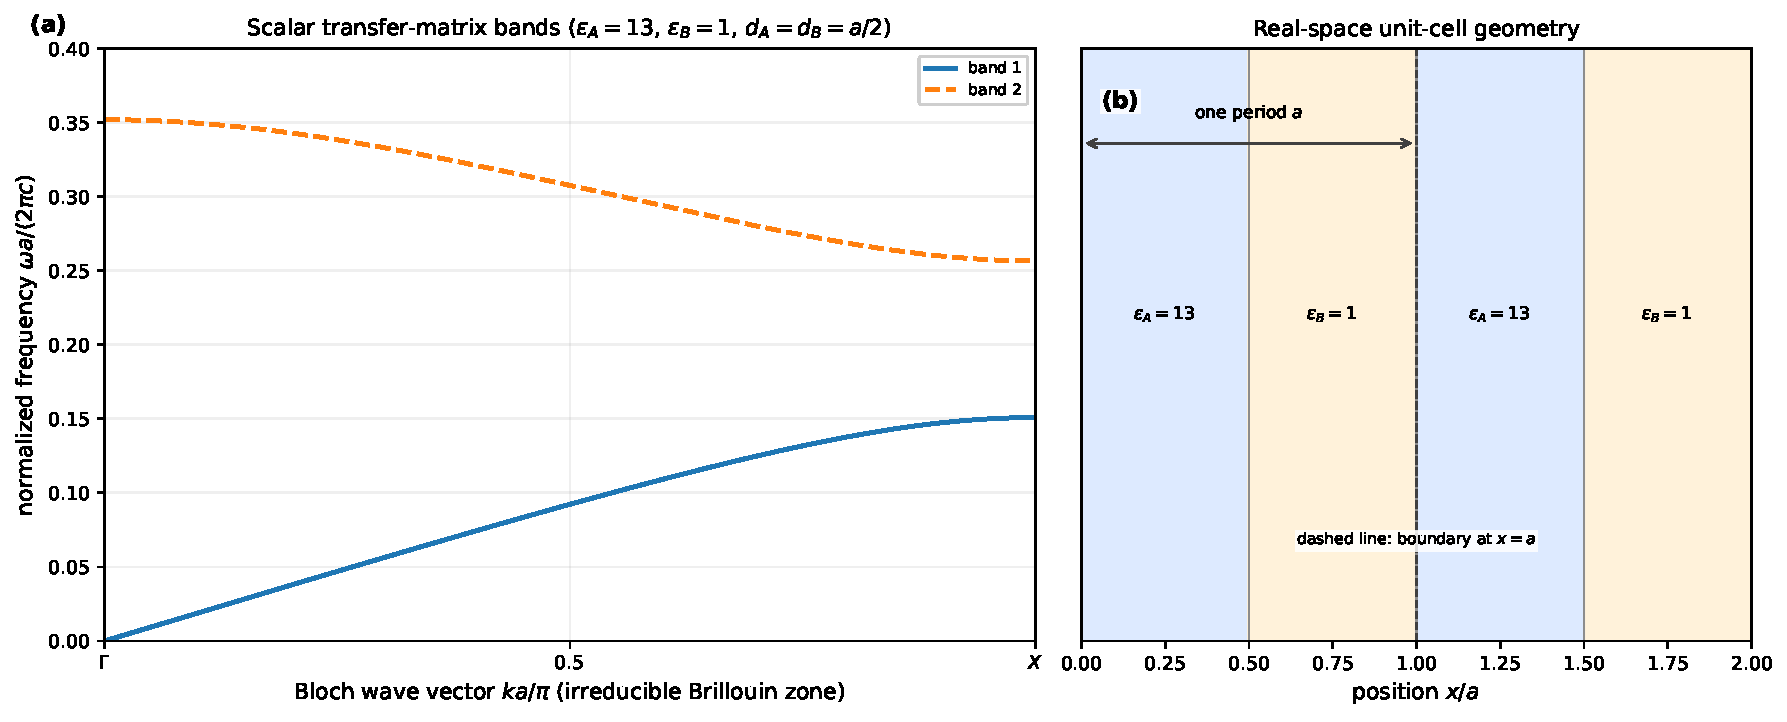
\includegraphics[width=0.98\textwidth]{fig_f1_1d_photonic_crystal_band.pdf}
 \caption{A one-dimensional Maxwell eigenproblem made visible. Panel (a) shows the Bloch band structure of a GaAs/air periodic stack computed from the transfer-matrix dispersion relation~\eqref{eq:1d-dispersion}; shaded regions mark band gaps where no real Bloch wave vector exists. Panel (b) sketches how the lower band-edge mode concentrates in the high-permittivity layers while the upper band-edge mode concentrates in the air layers, illustrating the variational principle of Section~\ref{sec:variational}.}
 \label{fig:ch1-1d-photonic-crystal-band}
\end{figure}

\subsection{What changes when $\varepsilon_B$ becomes complex}
\label{ssec:1d-complex}

If the air layers are replaced by a lossy material with
$\varepsilon_B = 1 + i\gamma$ ($\gamma > 0$ for loss with our
$e^{-i\omega t}$ convention), the transfer-matrix
elements become complex. At a fixed real driving frequency, the Bloch
wave vector $k$ acquires an imaginary part even inside the former pass
bands, so propagation is attenuated. Conversely, if one fixes a real
Bloch wave vector and solves the eigenvalue problem, the band frequencies
migrate into the complex-$\omega$ plane: every mode now decays in time.

If instead $\varepsilon_B = 1 - i\gamma$ (gain), the eigenfrequencies
move into the upper half of the complex plane and modes grow in time.
The balanced case $\varepsilon_A = \varepsilon_0 + i\gamma$,
$\varepsilon_B = \varepsilon_0 - i\gamma$ is a $\PT$-symmetric photonic
crystal (Chapter~\ref{ch:pt-symmetric}), where the interplay between gain
and loss produces a rich spectral structure including exceptional points
and spontaneous $\PT$-symmetry breaking.

This simple 1D example already contains, in embryo, most of the
non-Hermitian phenomena explored in this book. The rest of the
monograph develops the general theory, extends it to higher dimensions
and more complex geometries, and connects it to experimental observations
and device designs.


%% ================================================================
\section{Spectrum types: discrete, continuous, and complex}
\label{sec:spectrum-types}

The nature of the spectrum of $\Mop$ depends on the geometry and boundary
conditions. Understanding the taxonomy of spectra is essential because
different types of spectra require different mathematical tools and lead to
qualitatively different physics.

\paragraph{Closed cavities.}
A finite domain $\Omega$ with perfectly conducting walls supports a purely
discrete spectrum: an infinite sequence of real eigenfrequencies
$0 \le \omega_1 \le \omega_2 \le \cdots \to \infty$, each with finite
multiplicity. The corresponding eigenmodes form a complete orthonormal set
with respect to $\langle\cdot,\cdot\rangle$. This is the familiar
setting of microwave cavities and closed optical resonators.

The completeness of the eigenmodes means that any transverse field in the
cavity can be expanded as a convergent series in the eigenmodes:
\begin{equation}
 \HH(\rr) = \sum_{n=1}^{\infty} c_n\,\HH_n(\rr),
 \qquad c_n = \langle\HH_n,\,\HH\rangle.
 \label{eq:mode-expansion-closed}
\end{equation}
This expansion is the foundation of cavity QED, microwave filter design,
and the coupled-mode theory of Chapter~\ref{ch:maxwell-coupled-modes}.

\paragraph{Periodic media.}
A medium with discrete translational symmetry along one or more directions
admits Bloch's theorem (derived in Chapter~\ref{ch:periodicity}): the
eigenmodes are labeled by a continuous wave vector $\kk$ within the
Brillouin zone, and for each $\kk$ there is a discrete set of band
frequencies $\omega_n(\kk)$. The full spectrum is the union of these
bands and may contain gaps---frequency intervals with no propagating modes.
The band structure $\omega_n(\kk)$ is the central object of photonic-crystal
physics.

\paragraph{Open systems.}
When $\Omega$ extends to infinity---or equivalently, when we impose
outgoing-wave boundary conditions to model radiation loss---the spectrum
changes qualitatively. Besides possible guided modes (discrete, real
$\omega$), there is a continuous spectrum of radiation modes, and there may
be \emph{resonances}: solutions with complex $\omega$ in the lower half of
the complex frequency plane, describing fields that decay in time while
growing spatially toward infinity. These are the quasinormal modes of
Chapter~\ref{ch:qnm}. Their complex frequencies are the signature of
non-Hermiticity induced by openness.

The completeness of the mode expansion~\eqref{eq:mode-expansion-closed}
does not carry over straightforwardly to open systems. Quasinormal modes
diverge at spatial infinity and cannot be normalized with the standard inner
product. Chapter~\ref{ch:qnm} develops the regularization and
biorthogonal normalization that rescue the expansion, and
Chapter~\ref{ch:numerics} describes the numerical techniques (perfectly
matched layers, contour-integral eigensolvers) that make it practical.

\paragraph{Lossy or active media.}
Even for a closed cavity, if $\epsr$ has an imaginary part, the eigenvalue
$\omega^2/c^2$ becomes complex. For a medium with loss ($\Im\epsr > 0$
with our $e^{-i\omega t}$ convention), $\omega$ acquires a negative
imaginary part and modes decay; for a medium with gain ($\Im\epsr < 0$),
$\omega$ acquires a positive imaginary part and modes grow. The transition
from a purely real spectrum to a complex spectrum is the spectral
manifestation of non-Hermiticity.

\begin{figure}[t]
 \centering
 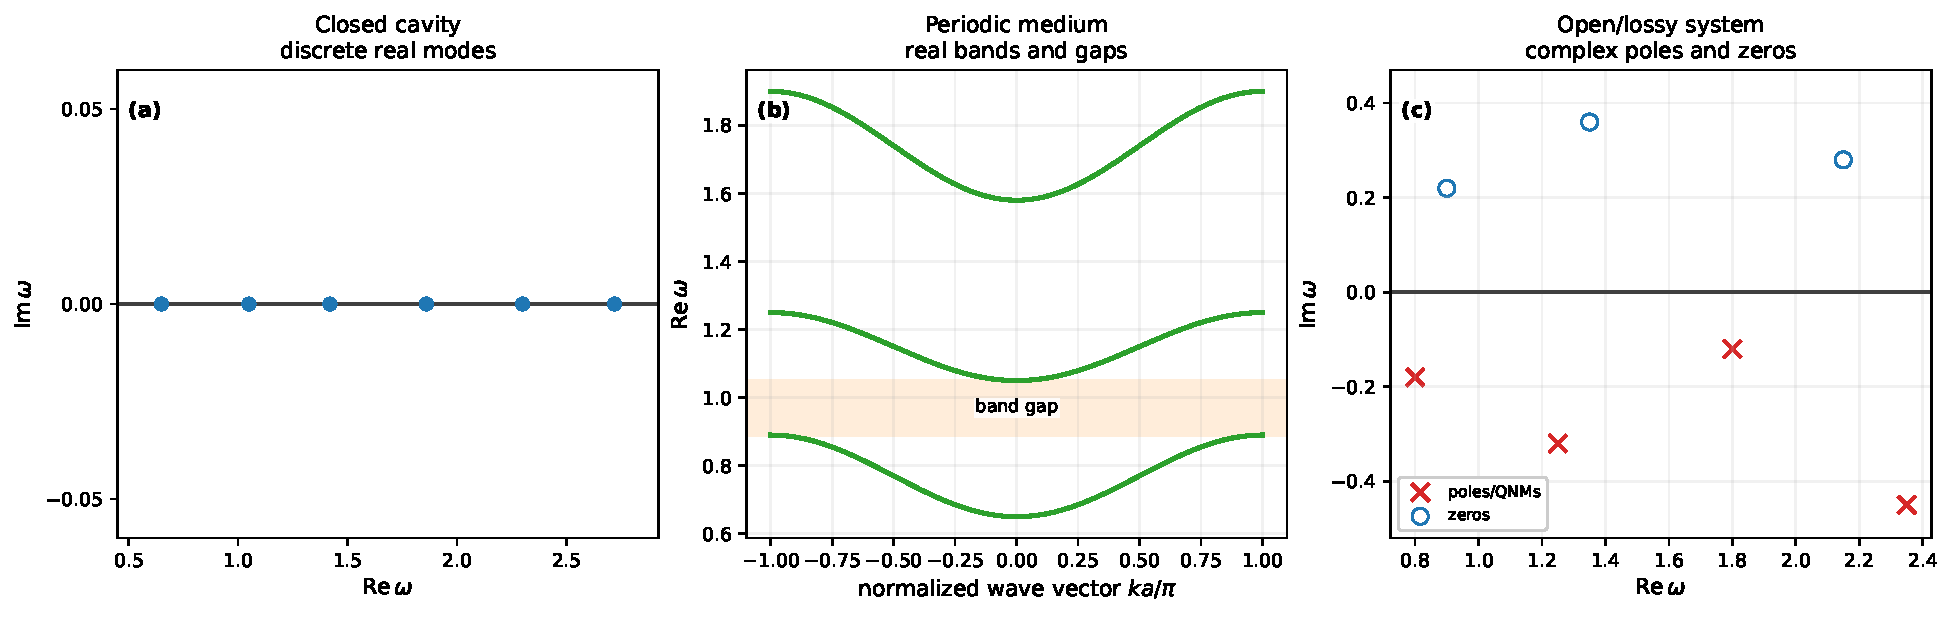
\includegraphics[width=0.98\textwidth]{fig_f1_spectrum_taxonomy.pdf}
 \caption{Three spectral regimes introduced in this opening chapter. A closed cavity has a discrete real spectrum; a periodic Hermitian medium has real bands and gaps; an open or lossy system is most naturally described by complex-frequency poles, zeros, and continua. The rest of the monograph develops the mathematical and physical consequences of moving from the first two panels to the third.}
 \label{fig:ch1-spectrum-taxonomy}
\end{figure}


%% ================================================================
\section{Positive semi-definiteness and the photonic density of states}
\label{sec:positive-dos}

The operator $\Mop$ on divergence-free fields with real, positive $\epsr$
is positive semi-definite:
\begin{equation}
 \langle\HH,\,\Mop\HH\rangle
 = \int_\Omega \frac{1}{\epsr(\rr)}\,|\curl\HH(\rr)|^2\;\dd^3 r
 \ge 0,
 \label{eq:positive-def}
\end{equation}
with equality if and only if $\curl\HH = 0$. After static harmonic fields
are removed by the boundary conditions or projected out, this implies
$\HH = 0$ on the dynamical transverse subspace. The nonzero eigenvalues
$\omega_n^2/c^2$ are therefore positive, and the corresponding
eigenfrequencies $\omega_n$ are real and positive.

The distribution of eigenfrequencies defines the \emph{photonic density
of states} (PDOS):
\begin{equation}
 \rho(\omega) = \sum_n \delta(\omega - \omega_n),
 \label{eq:pdos}
\end{equation}
which counts the number of modes per unit frequency interval. In a
homogeneous 3D medium with permittivity $\varepsilon$, the PDOS is
\begin{equation}
 \rho(\omega) = \frac{\varepsilon^{3/2}\,\omega^2}{\pi^2 c^3}
 \quad (\text{per unit volume}),
 \label{eq:pdos-bulk}
\end{equation}
which is the photonic analogue of Weyl's law for the Laplacian. The PDOS
is modified by photonic crystals (band gaps produce zeros in the PDOS) and
by cavities (the PDOS is enhanced at resonant frequencies), and these
modifications are the basis for controlling spontaneous emission
(Purcell effect), photon localization, and optical gain.

\begin{figure}[t]
 \centering
 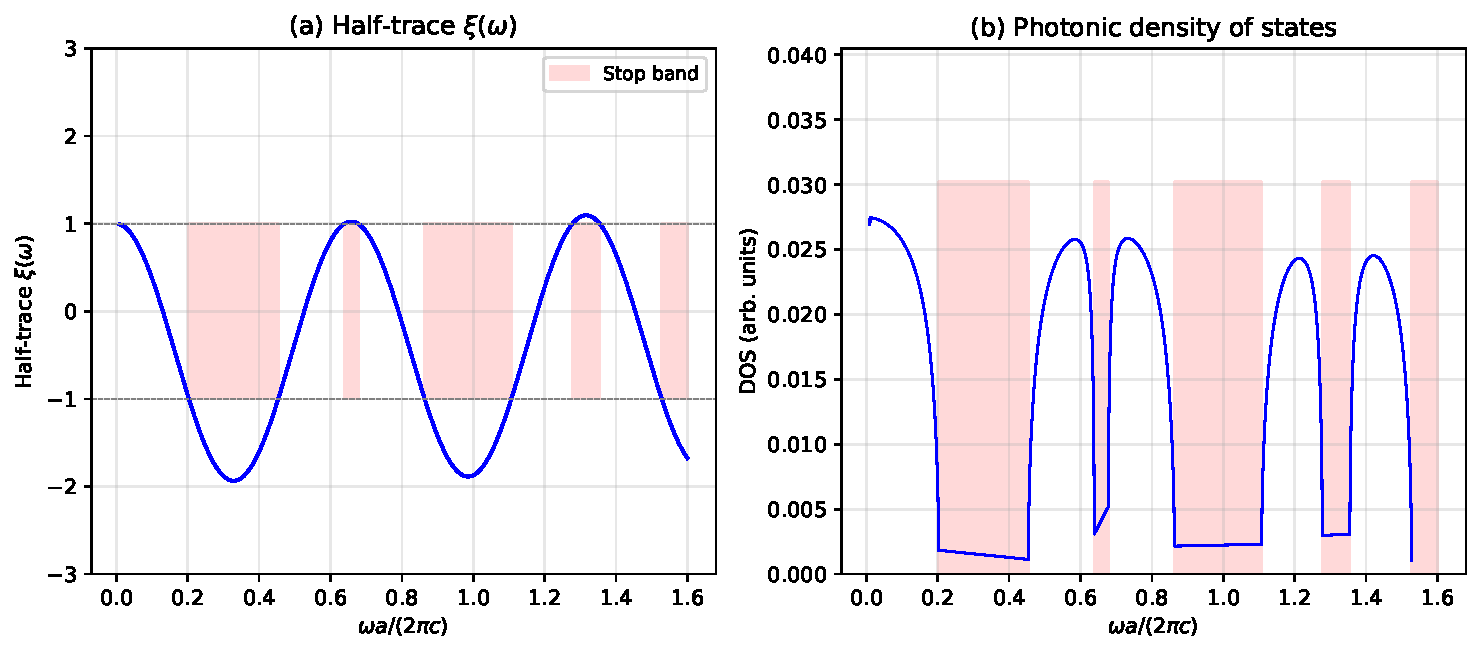
\includegraphics[width=0.85\linewidth]{figures/fig_f01_photonic_dos.pdf}
 \caption{Photonic density of states for a one-dimensional periodic
 dielectric. (a)~The transfer-matrix half-trace $\xi(\omega)$ divides
 pass bands ($|\xi|<1$) from stop bands ($|\xi|>1$). (b)~The density
 of states vanishes in stop bands and develops van-Hove enhancements
 near band edges, illustrating how Maxwell eigenvalue spectra differ
 qualitatively from free-space mode counting.}
 \label{fig:photonic-dos}
\end{figure}

When $\epsr$ becomes complex, the PDOS must be generalized to account for
the finite linewidth of the modes. The local density of states (LDOS)
at position $\rr_0$ is related to the imaginary part of the Green tensor:
\begin{equation}
 \rho(\rr_0, \omega) = \frac{2\omega}{\pi c^2}\,
 \Im\!\bigl[\tr \mathbf{G}(\rr_0, \rr_0; \omega)\bigr],
 \label{eq:ldos-green}
\end{equation}
where $\mathbf{G}$ is the dyadic Green tensor of the Maxwell system.
Chapter~\ref{ch:qnm} shows how the Green tensor can be expanded in terms
of quasinormal modes, providing a modal decomposition of the LDOS even
in open, non-Hermitian systems.


%% ================================================================
\section{What this book will build}
\label{sec:overview}

The rest of this monograph develops the consequences of the spectral
structure introduced here. Part~I continues by establishing the energy
inner products and reciprocity relations that underpin Hermitian photonics
(Chapter~\ref{ch:energy-inner}), deriving the Bloch band structure of
periodic media (Chapter~\ref{ch:periodicity}), and introducing the
scattering framework for open systems (Chapter~\ref{ch:boundaries}).

Part~II identifies the physical origins of non-Hermiticity:
material loss and gain (Chapter~\ref{ch:loss-gain-dispersion}),
radiation-induced complex eigenfrequencies in quasinormal modes
(Chapter~\ref{ch:qnm}), and the projection from the full Maxwell
operator to finite-dimensional coupled-mode models
(Chapter~\ref{ch:maxwell-coupled-modes}).

Part~III examines the most striking consequences of non-Hermitian operators:
exceptional points where eigenvectors coalesce
(Chapter~\ref{ch:exceptional-points}), $\PT$-symmetric optics
(Chapter~\ref{ch:pt-symmetric}), and the interplay of scattering poles
and zeros that connects lasers to coherent perfect absorbers
(Chapter~\ref{ch:poles-zeros}).

Part~IV builds the topological theory~\cite{icon2019rev,haldane2008possible}, starting from Berry curvature
derived directly from Maxwell fields (Chapter~\ref{ch:berry-maxwell}),
extending to complex bands and non-Hermitian gaps
(Chapter~\ref{ch:complex-bands}), developing photonic point-gap topology
(Chapter~\ref{ch:point-gap}), the skin effect and non-Bloch band theory
(Chapter~\ref{ch:skin-effect}), the reconstruction of bulk-boundary
correspondence (Chapter~\ref{ch:bbc-rebuilt}), and the topology of
bound states in the continuum (Chapter~\ref{ch:bic-topology}).

Part~V addresses computation (Chapter~\ref{ch:numerics}), devices and
physical limits (Chapter~\ref{ch:devices}), and open problems
(Chapter~\ref{ch:open-problems}).

Throughout, we shall insist on a single discipline: every non-Hermitian
structure must be traceable to a property of the Maxwell operator, not
merely asserted by analogy with a tight-binding Hamiltonian. This
Maxwell-first perspective is what gives the monograph its coherence and,
we hope, its lasting value.

\chapter{Energy, Inner Products, and Hermiticity}
\label{ch:energy-inner}

\begin{chapterlead}
Before we can say what non-Hermitian photonics \emph{is}~\cite{ozawa2018topological,bergholtz2019exceptional}, we must understand
what it \emph{is not}. The entire machinery of lossless electromagnetism---real
eigenfrequencies, orthogonal modes, energy conservation, reciprocity---rests
on a single mathematical fact: the Maxwell curl--curl operator is self-adjoint
with respect to an energy inner product. That inner product is derived
from the Poynting theorem, leading to the self-adjointness conditions
and catalogs the physical mechanisms that destroy them. Every later chapter
of this book is, in one way or another, a study of the consequences of that
destruction.
\end{chapterlead}


%% ================================================================
\section{Poynting's theorem}
\label{sec:poynting}

We begin, as always, from Maxwell's equations. Taking the dot product of
Faraday's law~\eqref{eq:faraday} with $\HH$ and of Amp\`ere's
law~\eqref{eq:ampere} with $\EE$, and subtracting, one obtains the
\emph{Poynting identity} in its instantaneous, differential form:
\begin{equation}
 \boxed{
 \divg\mathbf{S}
 = -\EE\cdot\pdv{\DD}{t} - \HH\cdot\pdv{\BB}{t},
 }
 \label{eq:poynting-diff}
\end{equation}
where the Poynting vector is
\begin{equation}
 \mathbf{S} = \EE\times\HH,
 \label{eq:poynting-vector}
\end{equation}
At this stage, \eqref{eq:poynting-diff} is only an identity: it follows
from Maxwell's equations alone and makes no assumption about the
constitutive relations. An energy density appears only after the material
response is specified well enough that
$\EE\cdot\partial_t\DD+\HH\cdot\partial_t\BB$ can be written as a total
time derivative.

For a \emph{nondispersive, lossless} medium with real, frequency-independent
$\epsr(\rr)$ and $\mur(\rr)$, the right-hand side simplifies:
\begin{equation}
 \EE\cdot\pdv{\DD}{t} + \HH\cdot\pdv{\BB}{t}
 = \pdv{}{t}\!\left[
 \frac{1}{2}\epsvac\epsr|\EE|^2
 + \frac{1}{2}\muvac\mur|\HH|^2
 \right].
 \label{eq:u-nondispersive}
\end{equation}
The energy density is therefore
\begin{equation}
 u(\rr,t) = \frac{1}{2}\epsvac\epsr(\rr)\,|\EE(\rr,t)|^2
 + \frac{1}{2}\muvac\mur(\rr)\,|\HH(\rr,t)|^2,
 \label{eq:energy-density}
\end{equation}
and the Poynting theorem becomes a local conservation law:
\begin{equation}
 \pdv{u}{t} + \divg\mathbf{S} = 0.
 \label{eq:energy-conservation}
\end{equation}
Integrating over a volume $\Omega$ bounded by a surface $\partial\Omega$,
\begin{equation}
 \dv{}{t}\int_\Omega u\;\dd^3 r
 = -\oint_{\partial\Omega}\mathbf{S}\cdot\nn\;\dd S.
 \label{eq:energy-integral}
\end{equation}
The total electromagnetic energy in $\Omega$ changes only through the Poynting
flux through its boundary. No energy is created or destroyed inside the
volume. This is the physical content of ``lossless'': energy is a
conserved quantity.

\paragraph{Example: energy balance in a lossy dielectric slab.}
Consider a plane wave $\EE = E_0\,e^{i(kz-\omega t)}\hat{\mathbf{x}}$
propagating in a slab of thickness $d$ with complex permittivity
$\epsr = \epsr' + i\epsr''$. To isolate absorption from interface
reflection, take $E_0$ below to denote the forward field just inside an
impedance-matched slab. The time-averaged Poynting flux entering the
material is then $S_{\mathrm{in}} = |E_0|^2/(2\eta)$, where
$\eta = \sqrt{\muvac/(\epsvac\epsr')}$ in the weak-loss limit.
Inside the slab, the field decays approximately as
$|\EE(z)|^2 = |E_0|^2 e^{-2\alpha z}$, where the attenuation constant
is $\alpha = (\omega/c)\Im\sqrt{\epsr}$. The time-averaged dissipated
power per unit area is
\begin{equation}
 P_{\mathrm{diss}} = \frac{\omega\epsvac\epsr''}{2}
 \int_0^d |E_0|^2 e^{-2\alpha z}\;\dd z
 = \frac{\omega\epsvac\epsr''\,|E_0|^2}{4\alpha}
 \bigl(1 - e^{-2\alpha d}\bigr).
 \label{eq:slab-dissipation}
\end{equation}
The Poynting flux exiting the slab is
$S_{\mathrm{out}} = S_{\mathrm{in}}\,e^{-2\alpha d}$ in the same weak-loss
description. Equivalently, the local identity
$-\mathrm{d}S/\mathrm{d}z =
(\omega\epsvac\epsr''/2)|E(z)|^2$ gives
$S_{\mathrm{in}} - S_{\mathrm{out}} = P_{\mathrm{diss}}$: the energy
lost from the wave equals the energy absorbed by the medium. With
interfaces included, reflected fluxes must also be counted, but the same
Poynting balance holds exactly.

When $\epsr'' < 0$ (gain medium), $\alpha < 0$ and the field grows
exponentially. The ``dissipated'' power is negative---the medium
delivers energy to the wave. The Poynting flux \emph{increases}
across the slab, and $S_{\mathrm{out}} > S_{\mathrm{in}}$. This
simple example illustrates the core physical mechanism behind all
non-Hermitian photonic phenomena: the energy inner product is no
longer conserved when $\epsr'' \neq 0$.

Figure~\ref{fig:ch2-poynting-slab} illustrates this energy balance for
two independent slabs.

\begin{figure}[t]
 \centering
 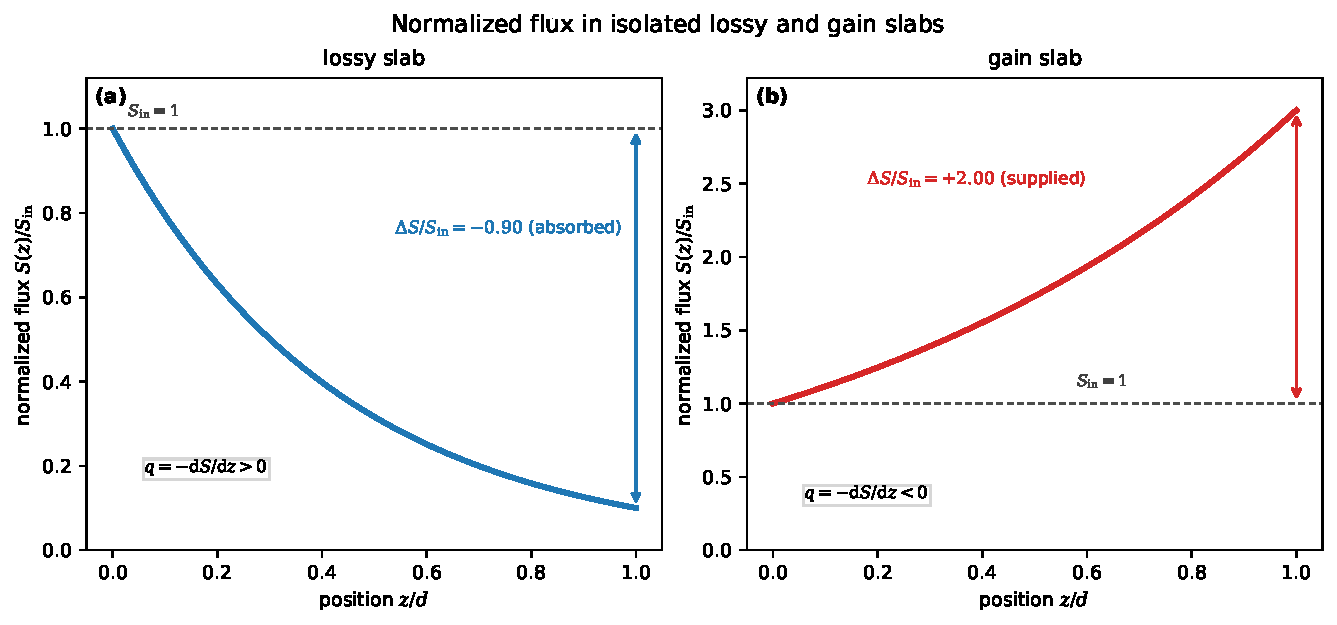
\includegraphics[width=0.95\linewidth]{fig_f2_poynting_slab_balance.pdf}
 \caption{Normalised Poynting flux $S(z)/S_{\mathrm{in}}$ through two
 independent dielectric slabs on separate vertical scales.
 (a)~Lossy slab ($\epsr''>0$): the flux decays exponentially from
 $S_{\mathrm{in}}=1$ to $S_{\mathrm{out}}=0.10$, so the medium
 absorbs $\Delta S/S_{\mathrm{in}}=0.90$. The sign convention
 $q=-\mathrm{d}S/\mathrm{d}z>0$ confirms that power density flows
 from the field into the material.
 (b)~Gain slab ($\epsr''<0$): the flux grows to
 $S_{\mathrm{out}}=3.00$, so the medium supplies
 $\Delta S/S_{\mathrm{in}}=2.00$ to the wave, with
 $q=-\mathrm{d}S/\mathrm{d}z<0$. In both panels, the dashed line
 marks $S_{\mathrm{in}}=1$ and the arrow at $z=d$ indicates the
 total flux change. The energy balance
 $S_{\mathrm{in}}-S_{\mathrm{out}}=\int_0^d q\,\mathrm{d}z$ is exact
 and follows directly from Poynting's theorem~\eqref{eq:poynting-diff}.}
 \label{fig:ch2-poynting-slab}
\end{figure}

\begin{booknote}[Units and conventions]
SI units are used throughout. The vacuum permittivity $\epsvac$ and
permeability $\muvac$ appear explicitly, so that $\epsr$ and $\mur$ are
dimensionless. The time convention is $e^{-i\omega t}$ for harmonic
fields. With this convention, a passive lossy medium has
$\Im\epsr(\omega) > 0$.
\end{booknote}


%% ================================================================
\section{Time-averaged energy and the harmonic inner product}
\label{sec:time-averaged}

For monochromatic fields with harmonic time dependence
$\EE(\rr,t) = \Re[\EE(\rr)\,e^{-i\omega t}]$, the time-averaged energy
density is
\begin{equation}
 \langle u \rangle
 = \frac{1}{4}\epsvac\epsr(\rr)\,|\EE(\rr)|^2
 + \frac{1}{4}\muvac\mur(\rr)\,|\HH(\rr)|^2,
 \label{eq:time-avg-u}
\end{equation}
and the time-averaged Poynting vector is
\begin{equation}
 \langle\mathbf{S}\rangle
 = \frac{1}{2}\Re\!\bigl[\EE(\rr)\times\HH^*(\rr)\bigr].
 \label{eq:time-avg-S}
\end{equation}

These expressions are valid only when $\epsr$ and $\mur$ are real and
frequency-independent. For dispersive media, additional terms involving
$\dd\epsr/\dd\omega$ appear (the Brillouin formula), and for lossy media,
the time-averaged ``energy density'' is no longer uniquely defined from
the macroscopic fields alone---a point we shall return to in
Chapter~\ref{ch:loss-gain-dispersion}.

The positive-definiteness of $\langle u\rangle$ when $\epsr > 0$ and
$\mur > 0$ is crucial. It means that the electromagnetic energy defines a
norm on the space of field configurations, and hence an inner product.


%% ================================================================
\section{Inner products for the Maxwell eigenproblem}
\label{sec:inner-products}

The eigenvalue problems derived in Chapter~\ref{ch:light-eigenvalue} have
natural inner products dictated by the energy density.

\subsection{The $\HH$-field inner product}
\label{ssec:H-inner}

For the operator $\Mop$ defined in~\eqref{eq:maxwell-op-H}, the natural
inner product is
\begin{equation}
 \langle\HH_1,\,\HH_2\rangle
 = \int_\Omega \HH_1^*(\rr)\cdot\HH_2(\rr)\;\dd^3 r.
 \label{eq:H-inner}
\end{equation}
This is the standard $L^2$ inner product, unweighted, because the
eigenvalue equation $\Mop\HH = (\omega^2/c^2)\HH$ has the eigenvalue on
the right without a material weight (assuming $\mur = 1$).

\subsection{The $\EE$-field inner product}
\label{ssec:E-inner}

For the $\EE$-field equation~\eqref{eq:curlcurl-E}, the eigenvalue appears
multiplied by $\epsr(\rr)$, so the correct inner product is the
$\epsr$-weighted one introduced in \eqref{eq:inner-product}:
\begin{equation}
 \langle\EE_1,\,\EE_2\rangle_\eps
 = \int_\Omega \EE_1^*(\rr)\cdot\epsr(\rr)\,\EE_2(\rr)\;\dd^3 r.
 \label{eq:E-inner-repeat}
\end{equation}
This inner product is positive-definite precisely when $\epsr(\rr) > 0$
for scalar media, or when the permittivity tensor is Hermitian positive
definite in anisotropic media.

\begin{figure}[t]
 \centering
 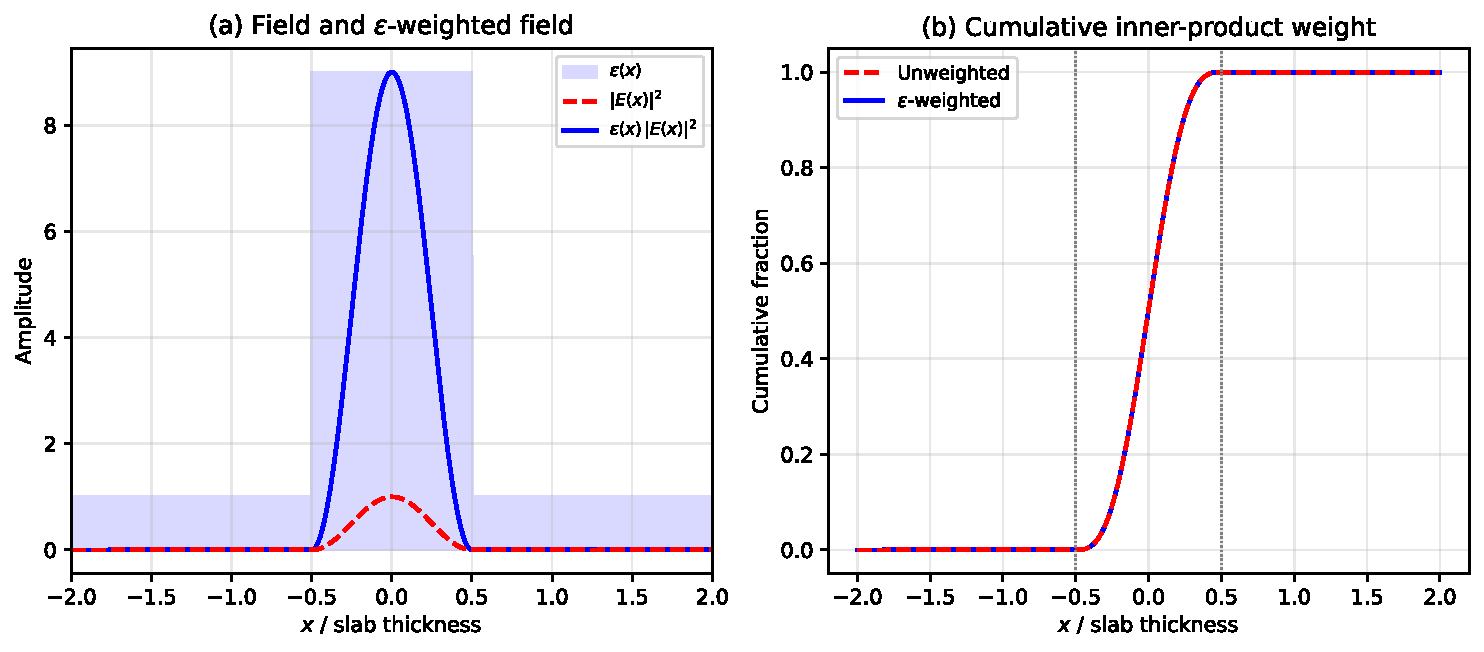
\includegraphics[width=0.85\linewidth]{figures/fig_f02_inner_product_weight.pdf}
 \caption{Visualisation of the $\varepsilon$-weighted inner product for
 a dielectric slab ($\varepsilon = 9$, shaded region).
 (a)~The bare field intensity $|E(x)|^2$ (red) and the
 $\varepsilon$-weighted intensity $\varepsilon(x)\,|E(x)|^2$ (blue).
 The weighting amplifies the contribution from the high-index region,
 reflecting the physical energy density $\frac{1}{2}\varepsilon_0
 \varepsilon|E|^2$.
 (b)~Cumulative inner-product weight: the $\varepsilon$-weighted
 curve (solid blue) rises steeply inside the slab, showing that most
 of the modal energy resides in the high-index material.}
 \label{fig:inner-product-weight}
\end{figure}


\subsection{The first-order Maxwell inner product}
\label{ssec:first-order-inner}

There is a third, often more natural, way to organize the Maxwell
eigenproblem. Writing the six-component field vector
$\mathbf{\Psi} = (\EE,\,\HH)^\transpose$,
the frequency-domain Maxwell equations~\eqref{eq:faraday-freq}--\eqref{eq:ampere-freq}
become a first-order system
\begin{equation}
 \underbrace{
 \begin{pmatrix}
 0 & i\curl \\[3pt]
 -i\curl & 0
 \end{pmatrix}
 }_{\displaystyle\hat{\mathcal{M}}}
 \begin{pmatrix} \EE \\ \HH \end{pmatrix}
 = \omega
 \underbrace{
 \begin{pmatrix}
 \epsvac\epsr & 0 \\[3pt]
 0 & \muvac\mur
 \end{pmatrix}
 }_{\displaystyle\hat{W}}
 \begin{pmatrix} \EE \\ \HH \end{pmatrix}.
 \label{eq:first-order-maxwell}
\end{equation}
The operator $\hat{\mathcal{M}}$ is manifestly Hermitian with respect to
the unweighted $L^2$ inner product (its off-diagonal blocks are related
by the curl identity~\eqref{eq:curl-ibp}). The generalized eigenvalue
problem $\hat{\mathcal{M}}\mathbf{\Psi} = \omega\,\hat{W}\mathbf{\Psi}$
is self-adjoint with respect to the energy inner product
\begin{equation}
 \langle\mathbf{\Psi}_1,\,\mathbf{\Psi}_2\rangle_W
 = \int_\Omega \mathbf{\Psi}_1^\adj\,\hat{W}\,\mathbf{\Psi}_2\;\dd^3 r
 = \int_\Omega\!\bigl[
 \epsvac\epsr\,\EE_1^*\cdot\EE_2
 + \muvac\mur\,\HH_1^*\cdot\HH_2
 \bigr]\dd^3 r,
 \label{eq:energy-inner-full}
\end{equation}
provided $\epsr$ and $\mur$ are real and positive and the boundary
conditions make the surface terms vanish. This inner product is
proportional to four times the time-averaged electromagnetic energy when
$\mathbf{\Psi}_1 = \mathbf{\Psi}_2$.

\paragraph{Comparing the three inner products on a concrete mode pair.}
To see how the three inner products differ in practice, consider the
fundamental TE$_{10}$ and TE$_{01}$ modes of a rectangular metallic
cavity ($a \times b \times d$) filled with a uniform dielectric
$\epsr = \mathrm{const}$, $\mur = 1$. The $\HH$-fields of these two
modes are $\HH_1 = H_0\cos(\pi x/a)\sin(\pi z/d)\,\hat{\mathbf{y}}$ and
$\HH_2 = H_0\sin(\pi y/b)\cos(\pi z/d)\,\hat{\mathbf{x}}$ (simplified for
illustration). The three inner products give:
\begin{enumerate}
 \item $\langle\HH_1,\HH_2\rangle = \int \HH_1^*\cdot\HH_2\;\dd^3r
 = 0$, because $\hat{\mathbf{x}}\cdot\hat{\mathbf{y}} = 0$ (orthogonal
 polarizations).
 \item $\langle\EE_1,\EE_2\rangle_\eps
 = \int \epsr\,\EE_1^*\cdot\EE_2\;\dd^3r = 0$, because the
 $\EE$-fields of the two modes have different spatial symmetries
 under the cavity's $C_{2v}$ group.
 \item $\langle\mathbf{\Psi}_1,\mathbf{\Psi}_2\rangle_W
 = \int(\epsvac\epsr\,\EE_1^*\cdot\EE_2
 + \muvac\,\HH_1^*\cdot\HH_2)\;\dd^3r = 0$, as both terms vanish
 independently.
\end{enumerate}
All three inner products agree (zero) for this mode pair in the
Hermitian case. The distinction matters only when $\epsr$ is complex
or when the modes are quasinormal: then the $\HH$-field inner product
stays unchanged (it does not involve $\epsr$), the $\EE$-field inner
product picks up an imaginary contribution from $\epsr''$, and the
first-order inner product mixes both. In non-Hermitian photonics~\cite{kawabata2018symmetry}, the
choice of inner product is not a convention but a physical decision
that determines orthogonality, completeness, and the meaning of
``energy.''

\begin{takeaway}[Energy as inner product]
The electromagnetic energy density defines the inner product that makes
the Maxwell operator self-adjoint. Making $\epsr$ complex, opening the
boundary, or projecting onto a subspace changes this inner product and
therefore changes the adjointness properties of the problem.
\end{takeaway}


%% ================================================================
\section{Self-adjointness: the complete argument}
\label{sec:self-adjoint-proof}

We now give a careful derivation of the self-adjointness of $\Mop$ in the
$\HH$-field formulation~\eqref{eq:maxwell-op-H}, which was stated without
full proof in Section~\ref{sec:self-adjoint}.

\begin{theorem}[Self-adjointness of $\Mop$]
\label{thm:self-adjoint}
Let $\Omega$ be a domain in $\mathbb{R}^3$ with piecewise smooth boundary
$\partial\Omega$. Let $\epsr(\rr)$ be real, positive, and bounded away
from zero, and let $\mur = 1$. Define
$\Mop\HH = \curl[\epsr^{-1}\curl\HH]$. Then $\Mop$ is self-adjoint with
respect to $\langle\cdot,\cdot\rangle$ on the space of divergence-free
fields satisfying either
(a)~$\nn\times\EE = 0$ on $\partial\Omega$ (perfect electric conductor),
or (b)~Bloch-periodic boundary conditions.
\end{theorem}

\begin{proof}
Consider two fields $\HH_1$ and $\HH_2$ in the domain of $\Mop$. We
compute
\begin{align}
 \langle\HH_1,\,\Mop\HH_2\rangle
 &= \int_\Omega \HH_1^*\cdot
 \curl\!\bigl[\epsr^{-1}\curl\HH_2\bigr]\;\dd^3 r.
 \label{eq:sa-step1}
\end{align}
Using the vector identity
$\mathbf{A}\cdot(\curl\mathbf{B})
 = (\curl\mathbf{A})\cdot\mathbf{B}
 + \divg(\mathbf{B}\times\mathbf{A})$
with $\mathbf{A} = \HH_1^*$ and
$\mathbf{B} = \epsr^{-1}\curl\HH_2$, we obtain
\begin{equation}
 \langle\HH_1,\,\Mop\HH_2\rangle
 = \int_\Omega \frac{1}{\epsr}\,
 (\curl\HH_1)^*\cdot(\curl\HH_2)\;\dd^3 r
 + \oint_{\partial\Omega}
 \bigl(\epsr^{-1}\curl\HH_2\times\HH_1^*\bigr)\cdot\nn\;\dd S.
 \label{eq:sa-step2}
\end{equation}
The bulk integral on the right is manifestly symmetric under the exchange
$1\leftrightarrow 2$ (with complex conjugation), because $\epsr^{-1}$ is
real. The surface integral vanishes under either boundary condition~(a)
or~(b).

For condition~(a), note that $\epsr^{-1}\curl\HH = (i\omega\epsvac)^{-1}\EE$
from Amp\`ere's law, so
$\nn\times(\epsr^{-1}\curl\HH) \propto \nn\times\EE = 0$
on $\partial\Omega$.

For condition~(b), the integrand on opposite faces of the unit cell
differs by Bloch phases $e^{i\kk\cdot\mathbf{a}}$ and $e^{-i\kk\cdot\mathbf{a}}$,
while the outward normals are opposite; the contributions cancel.

Since the bulk term is symmetric and the surface term vanishes,
\begin{equation}
 \langle\HH_1,\,\Mop\HH_2\rangle
 = \langle\Mop\HH_1,\,\HH_2\rangle,
 \label{eq:sa-result}
\end{equation}
completing the proof.
\end{proof}

The same argument can be repeated for the $\EE$-field
operator with the $\epsr$-weighted inner product, yielding
$\langle\EE_1,\,\Mop_E\EE_2\rangle_\eps
 = \langle\Mop_E\EE_1,\,\EE_2\rangle_\eps$
under the same boundary conditions.

\begin{remark}
The assumption that $\epsr$ is real enters at a precise point: the
symmetry of the bulk integral in~\eqref{eq:sa-step2}. If
$\epsr = \epsr' + i\epsr''$ with $\epsr'' \neq 0$, then
$1/\epsr^* \neq 1/\epsr$, the bulk term is no longer symmetric,
and self-adjointness fails. This is the mathematical origin of
non-Hermiticity from material loss or gain.
\end{remark}


%% ================================================================
\section{Consequences of self-adjointness}
\label{sec:sa-consequences}

When $\Mop$ is self-adjoint, the standard theorems of spectral theory for
compact self-adjoint operators in a Hilbert space apply. The consequences
are profound and familiar, but it is worth stating them explicitly, because
each one can fail in non-Hermitian photonics.

\subsection{Real eigenvalues}
\label{ssec:real-eigenvalues}

If $\Mop\HH_n = \lambda_n\HH_n$ with $\lambda_n = \omega_n^2/c^2$, then
\begin{equation}
 \lambda_n = \frac{\langle\HH_n,\,\Mop\HH_n\rangle}
 {\langle\HH_n,\,\HH_n\rangle}
 = \frac{\displaystyle\int_\Omega\epsr^{-1}|\curl\HH_n|^2\;\dd^3 r}
 {\displaystyle\int_\Omega|\HH_n|^2\;\dd^3 r}
 \;\ge\; 0.
 \label{eq:rayleigh-quotient}
\end{equation}
The eigenvalue $\lambda_n$ is real and non-negative: the eigenfrequencies
$\omega_n$ are real. There is no temporal decay, no growth, no complex
frequency.

\subsection{Orthogonality}
\label{ssec:orthogonality}

Eigenmodes belonging to distinct eigenvalues are orthogonal:
\begin{equation}
 \omega_m \neq \omega_n
 \quad\Longrightarrow\quad
 \langle\HH_m,\,\HH_n\rangle = 0.
 \label{eq:orthogonality}
\end{equation}
For the $\EE$-field formulation, the orthogonality relation is
$\langle\EE_m,\,\EE_n\rangle_\eps = 0$.

In either case, we may normalize the modes so that
$\langle\HH_m,\,\HH_n\rangle = \delta_{mn}$ or
$\langle\EE_m,\,\EE_n\rangle_\eps = \delta_{mn}$. Mode decompositions
and projections are then uniquely defined.

\subsection{Completeness}
\label{ssec:completeness}

For a compact domain (closed cavity), the eigenmodes form a complete
orthonormal basis. Any field satisfying the boundary conditions can be
expanded:
\begin{equation}
 \HH(\rr) = \sum_n c_n\,\HH_n(\rr),
 \qquad
 c_n = \langle\HH_n,\,\HH\rangle.
 \label{eq:completeness}
\end{equation}
The expansion coefficients $c_n$ are uniquely determined by the inner
product, and Parseval's identity
$\|\HH\|^2 = \sum_n |c_n|^2$ holds.

\subsection{Variational characterization}
\label{ssec:variational}

The eigenfrequencies can be obtained from the Rayleigh quotient:
\begin{equation}
 \omega_1^2/c^2
 = \min_{\HH\neq 0}\;
 \frac{\displaystyle\int\epsr^{-1}|\curl\HH|^2\;\dd^3 r}
 {\displaystyle\int|\HH|^2\;\dd^3 r},
 \label{eq:variational}
\end{equation}
with higher eigenvalues given by the min--max principle. This
characterization is the basis of numerical methods such as the plane-wave
expansion and finite-element eigensolvers used in photonic-crystal
computations~\cite{paz2019tutorial}.


%% ================================================================
\section{Lorentz reciprocity}
\label{sec:reciprocity}

Self-adjointness (Hermiticity) is not the only symmetry of the Maxwell
operator. There is a distinct and equally important property:
\emph{reciprocity}.

Consider two source--field pairs $(\JJ_a, \EE_a, \HH_a)$ and
$(\JJ_b, \EE_b, \HH_b)$ at the same frequency $\omega$ in a medium
with $\epsr(\rr)$ and $\mur(\rr)$ that are symmetric tensors (which
includes all isotropic and many anisotropic media). The Lorentz
reciprocity theorem states
\begin{equation}
 \int_\Omega\bigl(\EE_a\cdot\JJ_b - \EE_b\cdot\JJ_a\bigr)\;\dd^3 r
 = \oint_{\partial\Omega}
 \bigl(\EE_a\times\HH_b - \EE_b\times\HH_a\bigr)\cdot\nn\;\dd S.
 \label{eq:lorentz-reciprocity}
\end{equation}
If the surface integral vanishes (closed cavity, or sources far from
$\partial\Omega$), this reduces to the familiar statement
$\langle\EE_a,\JJ_b\rangle = \langle\EE_b,\JJ_a\rangle$:
swapping source and observation gives the same field projection.

\subsection{Reciprocity and the scattering matrix}
\label{ssec:reciprocity-smatrix}

Reciprocity has a direct and powerful consequence for the scattering
matrix $S(\omega)$ of Chapter~\ref{ch:boundaries}. If the medium is
reciprocal (symmetric $\epsr$ and $\mur$ tensors), then the $S$-matrix
satisfies
\begin{equation}
 S^\transpose(\omega) = S(\omega),
 \label{eq:s-reciprocity}
\end{equation}
i.e., $S$ is a symmetric matrix. This means that the transmission from
port $i$ to port $j$ equals the transmission from port $j$ to port $i$:
$S_{ij} = S_{ji}$.

The proof follows from the Lorentz reciprocity
theorem~\eqref{eq:lorentz-reciprocity}. Let $\EE_a$ be the field
produced by a source at port~$i$ and $\EE_b$ the field from a source at
port~$j$. If the surface integral vanishes (all ports are included in
the integration surface), then
$\langle\EE_a,\JJ_b\rangle = \langle\EE_b,\JJ_a\rangle$, which
translates directly into $S_{ij} = S_{ji}$ when expressed in the
scattering-matrix language.

This symmetry is \emph{not} the same as unitarity. A unitary $S$-matrix
($S^\dagger S = I$) expresses energy conservation and requires
Hermiticity; a symmetric $S$-matrix ($S^\transpose = S$) expresses
reciprocity and requires only symmetric material tensors. A lossy
dielectric cavity has $S^\transpose = S$ (reciprocal) but
$S^\dagger S \neq I$ (energy is absorbed). A magneto-optic material
breaks the tensor symmetry and therefore breaks both reciprocity and
$S$-matrix symmetry, even if the system is lossless.

The distinction between reciprocity (symmetric $S$) and Hermiticity
(unitary $S$) is the scattering-theory counterpart of the distinction
between the unconjugated bilinear form and the conjugate inner product
in the operator formulation.

\begin{booknote}[Reciprocity versus Hermiticity]
Reciprocity and Hermiticity are conceptually distinct.
\emph{Hermiticity} involves the complex-conjugate inner product
$\langle\mathbf{F}^*,\Mop\mathbf{G}\rangle$ and requires $\epsr$ to be
\emph{real}. \emph{Reciprocity} involves an unconjugated bilinear form
$(\mathbf{F},\sigma\mathbf{G})$ and requires $\epsr$ to be a
\emph{symmetric tensor}. A medium with complex $\epsr = \epsr' + i\epsr''$
that is scalar (or symmetric) is \emph{reciprocal but not Hermitian}.
This distinction is central to non-Hermitian photonics: many systems of
interest---lossy dielectrics, gain media, $\PT$-symmetric
structures---are reciprocal, even though they are not Hermitian.
The reaction-based inner product exploited in coupled-mode
theory~\cite{xu2015general} is built on reciprocity, not Hermiticity.
\end{booknote}


%% ================================================================
\section{Four roads to non-Hermiticity}
\label{sec:four-roads}

The self-adjointness proof of Section~\ref{sec:self-adjoint-proof} relied on
three assumptions: (i)~$\epsr$ real, (ii)~boundary terms vanish,
(iii)~fields live in a complete Hilbert space. The Rayleigh quotient
argument~\eqref{eq:rayleigh-quotient} additionally used $\epsr > 0$.
Violating any of these opens a distinct road to non-Hermitian physics.
Figure~\ref{fig:ch2-hermiticity-map} summarises the logical structure.

\begin{figure}[t]
 \centering
 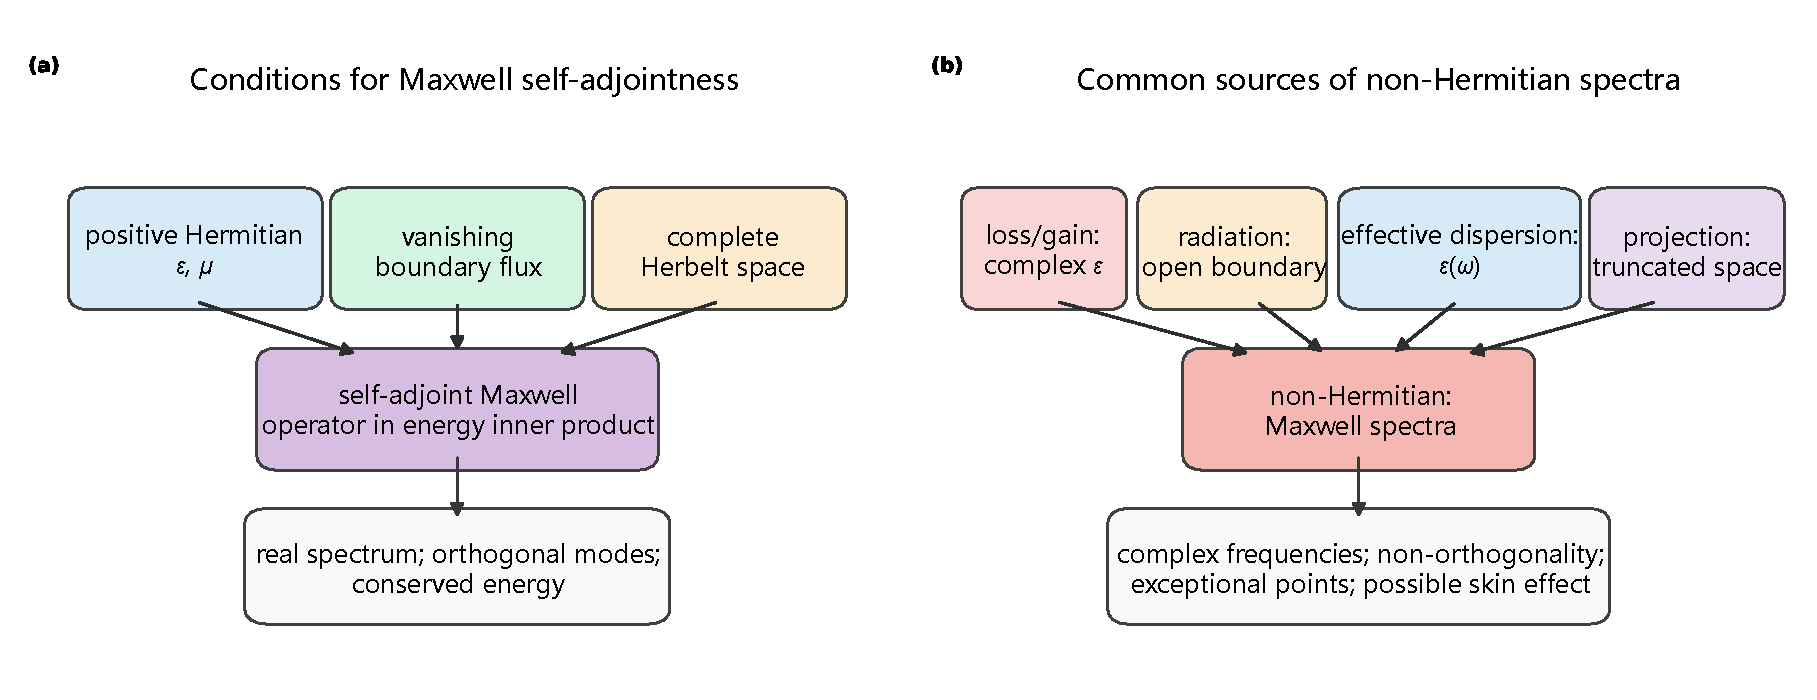
\includegraphics[width=0.92\linewidth]{fig_f2_hermiticity_conditions.pdf}
 \caption{Conditions for Maxwell self-adjointness and the four common
 mechanisms that break them.
 (a)~Three sufficient conditions---positive Hermitian constitutive
 tensors $\varepsilon,\mu$, vanishing boundary flux (closed domain),
 and a complete Hilbert space---ensure that the Maxwell curl-curl
 operator is self-adjoint in the energy inner product, yielding a
 real spectrum, orthogonal modes, and conserved electromagnetic
 energy.
 (b)~Each condition can be violated independently: material loss or
 gain introduces complex $\varepsilon$; radiation through open
 boundaries allows energy to leave the domain; frequency-dependent
 $\varepsilon(\omega)$ makes the operator effectively non-self-adjoint
 at any fixed real frequency; and projection onto a finite mode
 subspace discards completeness. The resulting non-Hermitian
 spectra exhibit complex eigenfrequencies, non-orthogonal modes,
 exceptional points, and possible skin-effect localisation---the
 subjects of Parts~II--IV of this monograph.}
 \label{fig:ch2-hermiticity-map}
\end{figure}


\subsection{Material loss and gain}
\label{ssec:road-lossgain}

If the permittivity has an imaginary part, $\epsr = \epsr' + i\epsr''$, the
factor $\epsr^{-1}$ in~\eqref{eq:sa-step2} is no longer real, and the bulk
integral loses its symmetry. For monochromatic fields in a nondispersive
medium, the time-averaged Poynting identity becomes
\begin{equation}
 \divg\langle\mathbf{S}\rangle
 = -\frac{\omega}{2}\epsvac\epsr''(\rr)\,|\EE(\rr)|^2.
 \label{eq:poynting-lossy}
\end{equation}
For $\epsr'' > 0$ (our $e^{-i\omega t}$ convention), energy is absorbed;
for $\epsr'' < 0$, energy is emitted. The eigenfrequencies become complex,
and modes are no longer orthogonal with respect to
$\langle\cdot,\cdot\rangle_\eps$.

\paragraph{Physical example: coupled whispering-gallery resonators.}
Two silica microsphere resonators (diameter $\sim 50\;\mu$m) coupled
evanescently through a sub-wavelength air gap provide a clean realisation.
When both spheres are passive (intrinsic material loss only,
$\epsr'' \sim 10^{-7}$), the system is nearly Hermitian: the two
whispering-gallery modes split into symmetric and antisymmetric
supermodes with real frequency splitting $2\kappa$. When one sphere is
doped with an erbium gain medium pumped above threshold ($\epsr'' < 0$),
the system becomes genuinely non-Hermitian: the two supermodes acquire
different imaginary parts, and at a critical pump power the frequency
splitting vanishes at an exceptional point. The transition from the
Hermitian regime ($\epsr'' = 0$) to the EP ($|\epsr''|$ reaches the
critical value) is a continuous deformation of the eigenvalue structure
that can be tracked experimentally through the transmission spectrum.

This mechanism is explored in Chapter~\ref{ch:loss-gain-dispersion} and
provides the physical basis for $\PT$-symmetric optics
(Chapter~\ref{ch:pt-symmetric}).

\subsection{Radiation and open boundaries}
\label{ssec:road-radiation}

For an open system, the outgoing-wave (Sommerfeld) boundary condition
replaces the standing-wave condition of a closed cavity. The surface
integral in~\eqref{eq:sa-step2} no longer vanishes: energy flows outward
through $\partial\Omega$. As a result, eigenfrequencies acquire negative
imaginary parts (fields decay in time while growing spatially toward
infinity). These are the quasinormal modes of Chapter~\ref{ch:qnm}.

\paragraph{Physical example: a dielectric microsphere in vacuum.}
A dielectric sphere of radius $R$ and $\epsr = 4$ (e.g., a glass
microsphere) supports whispering-gallery modes with $Q$ factors that
increase exponentially with the angular momentum $\ell$. Each mode has
a complex eigenfrequency $\omega_\ell = \omega_\ell' - i\gamma_\ell/2$,
where $\gamma_\ell$ is the radiative decay rate. Even though the
material is perfectly lossless ($\epsr'' = 0$), the eigenfrequencies are
complex because the outgoing-wave boundary condition at $r \to \infty$
breaks the self-adjointness of the Maxwell operator. The non-Hermiticity
is purely geometrical: it arises from the open boundary, not from any
material dissipation.

\subsection{Frequency dispersion}
\label{ssec:road-dispersion}

Even for a closed, passive medium, if $\epsr(\omega)$ depends on frequency,
the eigenproblem is nonlinear in $\omega$ and the simple inner product
\eqref{eq:E-inner-repeat} is no longer the correct energy functional.
The Brillouin formula
\begin{equation}
 \langle u\rangle_{\mathrm{disp}}
 = \frac{1}{4}\epsvac\,
 \dv{}{\omega}\bigl[\omega\,\epsr'(\omega)\bigr]\,|\EE|^2
 + \frac{1}{4}\muvac\,
 \dv{}{\omega}\bigl[\omega\,\mur'(\omega)\bigr]\,|\HH|^2
 \label{eq:brillouin}
\end{equation}
gives a partial answer for weakly dispersive, low-loss media, but it is not
a true inner product: it is not bilinear, it depends on $\omega$, and it
becomes negative near absorption resonances. A rigorous treatment requires
auxiliary fields that restore the Hamiltonian structure of the dispersive
Maxwell system~\cite{figotin2004hamiltonian}. We defer this construction to
Chapter~\ref{ch:loss-gain-dispersion}, where it will be developed in detail.

\paragraph{Example: why the naive inner product fails for a
Lorentz medium.}
Consider a single Lorentz oscillator with permittivity
\begin{equation}
 \epsr(\omega) = 1 + \frac{\omega_p^2}{\omega_0^2 - \omega^2 - i\gamma\omega},
 \label{eq:lorentz-ch2}
\end{equation}
where $\omega_0$ is the resonance frequency, $\omega_p$ is the plasma
frequency, and $\gamma$ is the damping rate. At a frequency
$\omega$ well below the resonance ($\omega \ll \omega_0$), the
permittivity is approximately real and the naive inner product
$\langle \FF, \GG \rangle = \int \epsr\,\FF^* \cdot \GG\;\dd^3 r$ is
positive-definite. The Brillouin energy density~\eqref{eq:brillouin}
reduces to $\langle u \rangle_{\mathrm{disp}} \approx
\frac{1}{4}\epsvac\,(1 + \omega_p^2/\omega_0^2)\,|\EE|^2$, which is
the expected electrostatic energy enhanced by the polarizability.

Near the resonance ($\omega \approx \omega_0$), the situation changes
dramatically. The real part $\epsr'(\omega)$ passes through zero and
becomes negative, while the imaginary part $\epsr''(\omega)$ peaks at
$\omega_0$. The naive inner product is no longer positive-definite:
$\epsr'|\EE|^2$ can be negative, and the ``norm'' of a mode can
vanish or change sign. This is not a mathematical pathology but a
physical fact: near a material resonance, the electromagnetic energy is
stored partly in the kinetic energy of the polarization current, not
only in the field. The Brillouin formula accounts for this by
including the derivative $\partial(\omega\epsr')/\partial\omega$:
\begin{equation}
 \dv{}{\omega}\bigl[\omega\,\epsr'(\omega)\bigr]
 = 1 + \omega_p^2\,\frac{\omega_0^2 + \omega^2}
 {(\omega_0^2 - \omega^2)^2 + \gamma^2\omega^2},
 \label{eq:brillouin-derivative}
\end{equation}
which is positive for all $\omega$ when $\gamma$ is small (the
no-gain condition). The Brillouin energy thus remains positive even
where $\epsr'$ itself is negative---the ``missing'' energy is stored in
the oscillating polarization.

However, for $\gamma$ comparable to $\omega_0$ (strongly damped media),
the Brillouin formula itself becomes unreliable, and one must resort to
the auxiliary-field Hamiltonian embedding of
Chapter~\ref{ch:loss-gain-dispersion}, where the polarization degrees
of freedom are treated as dynamical variables on the same footing as the
electromagnetic field. This construction restores a true inner product
at the cost of enlarging the Hilbert space, and it is the key technical
step that makes the non-Hermitian Maxwell eigenproblem well-posed for
dispersive media.

\paragraph{Comparing inner products: lossless versus dispersive.}
The following table summarises the three regimes:
\begin{center}
\begin{tabular}{lcc}
 \hline
 \textbf{Regime} & \textbf{Weight} & \textbf{Positive-definite?} \\
 \hline
 Non-dispersive ($\epsr$ real, constant) &
 $\epsr\,|\EE|^2$ & Yes \\
 Weakly dispersive ($\gamma \ll \omega_0$) &
 $\partial_\omega(\omega\epsr')\,|\EE|^2$ & Yes \\
 Strongly dispersive ($\gamma \sim \omega_0$) &
 Auxiliary-field Hamiltonian & Yes (enlarged space) \\
 \hline
\end{tabular}
\end{center}
This table reflects the central message of Chapter~\ref{ch:energy-inner}:
as the medium becomes more realistic, the inner product that makes the
Maxwell operator self-adjoint becomes more complex, and the price of
restoring Hermiticity is paid either by restricting the frequency range
or by enlarging the state space.

\subsection{Projection onto a subspace}
\label{ssec:road-projection}

Even when the full Maxwell operator is self-adjoint, restricting attention
to a finite number of resonant modes creates an effective Hamiltonian that
is generically non-Hermitian. The discarded modes act as an environment:
they carry away energy (through radiation or absorption in modes outside
the truncated subspace) and introduce complex corrections to the effective
eigenvalues. The Petermann excess-noise factor, which quantifies the
nonorthogonality of laser modes, is a direct consequence of this
projection~\cite{kristensen2011effective}.

This mechanism is the subject of Chapter~\ref{ch:maxwell-coupled-modes},
where effective non-Hermitian Hamiltonians are derived from Maxwell
field theory rather than postulating them.

\paragraph{Physical example: few-mode fibre.}
A single-mode optical fibre supports one guided mode per polarization.
When this mode couples to a nearby scatterer (a nanoparticle, a
microring, or a Bragg grating), the coupled system has two or three
resonant modes, but the radiation continuum acts as an infinite
environment. Projecting the full Maxwell problem onto the two-mode
subspace yields an effective $2\times 2$ non-Hermitian Hamiltonian
whose off-diagonal elements include both the direct coupling and a
radiative shift from the discarded continuum. The Petermann factor of
the coupled modes measures how far the projected eigenvectors deviate
from orthogonality---a direct consequence of the incomplete Hilbert
space.

\begin{takeaway}[Four mechanisms, one mathematical origin]
Material loss/gain makes the weight $\epsr$ complex.
Radiation makes the boundary terms nonzero.
Dispersion makes the eigenproblem nonlinear in $\omega$ unless additional
material degrees of freedom are included.
Projection makes the Hilbert space incomplete.
All four destroy self-adjointness of the Maxwell operator, but they do so
in physically distinct ways and lead to different spectral and topological
consequences.
\end{takeaway}


%% ================================================================
\section{The structure of what follows}
\label{sec:ch2-forward}

The Hermitian baseline established in this chapter---energy inner product,
self-adjointness, real eigenvalues, orthogonal modes, reciprocity---is the
standard against which every non-Hermitian phenomenon in the rest of this
book will be measured.

Chapter~\ref{ch:periodicity} extends the self-adjoint framework to periodic
media, where Bloch's theorem organizes the spectrum into bands.
Chapter~\ref{ch:boundaries} introduces open systems and the scattering
matrix, setting the stage for quasinormal modes.

In Part~II, each of the four roads identified above~\cite{gong2018topological,icon2021exceptional} will be explored in
depth: material loss, gain, and dispersion in
Chapter~\ref{ch:loss-gain-dispersion}; quasinormal modes from radiation in
Chapter~\ref{ch:qnm}; and projection to coupled-mode models in
Chapter~\ref{ch:maxwell-coupled-modes}.

\begin{figure}[t]
 \centering
 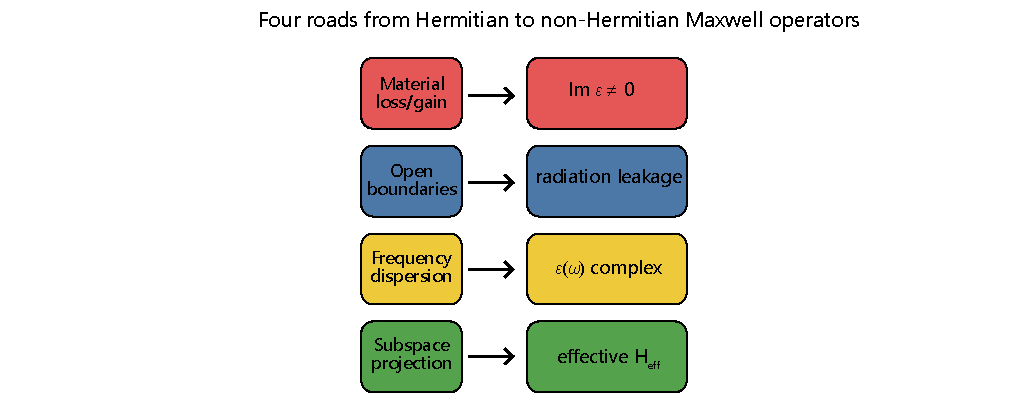
\includegraphics[width=0.78\linewidth]{fig_f2_four_roads.pdf}
 \caption{Four roads from Hermitian to non-Hermitian Maxwell
 operators. Each mechanism independently breaks the
 self-adjointness of the curl--curl operator $\Theta$:
 material loss or gain ($\Im\varepsilon \neq 0$),
 open boundaries allowing radiation leakage,
 frequency dispersion making $\varepsilon(\omega)$ complex,
 and subspace projection yielding an effective non-Hermitian
 Hamiltonian. Many photonic systems exhibit several roads
 simultaneously. Each road is explored in depth in
 Parts~II--V of this book.}
 \label{fig:four-roads-nh}
\end{figure}

The reader who is already familiar with Hermitian electromagnetism may
wish to proceed directly to Chapter~\ref{ch:loss-gain-dispersion}.
However, we recommend at least reviewing the distinction between
reciprocity and Hermiticity in Section~\ref{sec:reciprocity} and the four
roads in Section~\ref{sec:four-roads}, as these ideas recur throughout the
non-Hermitian parts of the book.

\chapter{Periodicity and Photonic Bands}
\label{ch:periodicity}

\begin{chapterlead}
A homogeneous dielectric has a continuous spectrum: any frequency can
propagate. Introduce a periodic modulation of the permittivity and the
spectrum reorganizes into bands separated by gaps---frequency windows in
which no propagating mode exists. The band structure of photonic
crystals is derived directly from the Maxwell eigenproblem of
Chapter~\ref{ch:light-eigenvalue}, using Bloch's theorem as the organizing
principle. The real, orthogonal, gapped band structure established here is
the Hermitian baseline against which all non-Hermitian modifications in
later chapters will be measured.
\end{chapterlead}


%% ================================================================
\section{Periodic permittivity and the direct lattice}
\label{sec:periodic-eps}

Consider a medium whose relative permittivity is periodic:
\begin{equation}
 \epsr(\rr + \mathbf{R}) = \epsr(\rr)
 \qquad\text{for all lattice vectors}\quad
 \mathbf{R} = n_1\mathbf{a}_1 + n_2\mathbf{a}_2 + n_3\mathbf{a}_3,
 \label{eq:periodic-eps}
\end{equation}
where $\mathbf{a}_1, \mathbf{a}_2, \mathbf{a}_3$ are primitive lattice
vectors and $n_i \in \mathbb{Z}$. We assume $\epsr(\rr)$ is real,
positive, and bounded, so the self-adjointness results of
Chapter~\ref{ch:energy-inner} apply within each unit cell.

The set of all lattice vectors $\mathbf{R}$ forms the \emph{direct
lattice}. The primitive unit cell $\Omega_{\mathrm{uc}}$ can be chosen
as the parallelotope spanned by $\{\mathbf{a}_i\}$ or, more symmetrically,
as the Wigner--Seitz cell centered on a lattice point.

For most of this chapter we work in two dimensions, where the permittivity
$\epsr(x,y)$ is periodic in the $(x,y)$ plane and uniform along $z$.
This covers ideal two-dimensional photonic crystals---arrays of dielectric
rods or air holes uniform along the third direction---and gives a useful
starting point for slab photonic crystals when vertical confinement can be
treated separately. It also allows the TE/TM decomposition of
Section~\ref{sec:2d-reductions}. The extension to fully three-dimensional
crystals is conceptually straightforward but notationally heavier;
see~\cite{paz2019tutorial} for explicit three-dimensional calculations.


%% ================================================================
\section{Reciprocal lattice and Brillouin zone}
\label{sec:reciprocal}

The \emph{reciprocal lattice} is defined by vectors $\GG$ satisfying
$e^{i\GG\cdot\mathbf{R}} = 1$ for all direct-lattice vectors $\mathbf{R}$.
In two dimensions, the primitive reciprocal-lattice vectors
$\mathbf{b}_1, \mathbf{b}_2$ satisfy
\begin{equation}
 \mathbf{a}_i \cdot \mathbf{b}_j = 2\pi\,\delta_{ij},
 \qquad i,j = 1,2.
 \label{eq:reciprocal-vectors}
\end{equation}
The first \emph{Brillouin zone} (BZ) is the Wigner--Seitz cell of the
reciprocal lattice. It is the fundamental domain for the wave vector
$\kk$: any $\kk$ outside the first BZ can be mapped back into it by
subtracting a reciprocal-lattice vector.

\begin{example}[Square and triangular lattices]
For a square lattice with period $a$, the primitive vectors are
$\mathbf{a}_1 = a\hat{x}$, $\mathbf{a}_2 = a\hat{y}$, and the
reciprocal-lattice vectors are $\mathbf{b}_1 = (2\pi/a)\hat{x}$,
$\mathbf{b}_2 = (2\pi/a)\hat{y}$. The first BZ is a square of side
$2\pi/a$ centered at the origin.

For a triangular lattice with $\mathbf{a}_1 = a\hat{x}$,
$\mathbf{a}_2 = a(\hat{x}/2 + \sqrt{3}\hat{y}/2)$, the BZ is a regular
hexagon. Its high-symmetry points---$\Gamma$, $M$, $K$---play a
central role in photonic-crystal band diagrams.
\end{example}

Figure~\ref{fig:ch3-reciprocal-lattice-bz} fixes the reciprocal-space
geometry that will be used throughout the chapter. The important point is
not the artistic shape of the cell, but the convention: the first BZ is a
Wigner--Seitz cell of the reciprocal lattice, and the red curves are
standard high-symmetry paths used to display bands.

\begin{figure}[t]
 \centering
 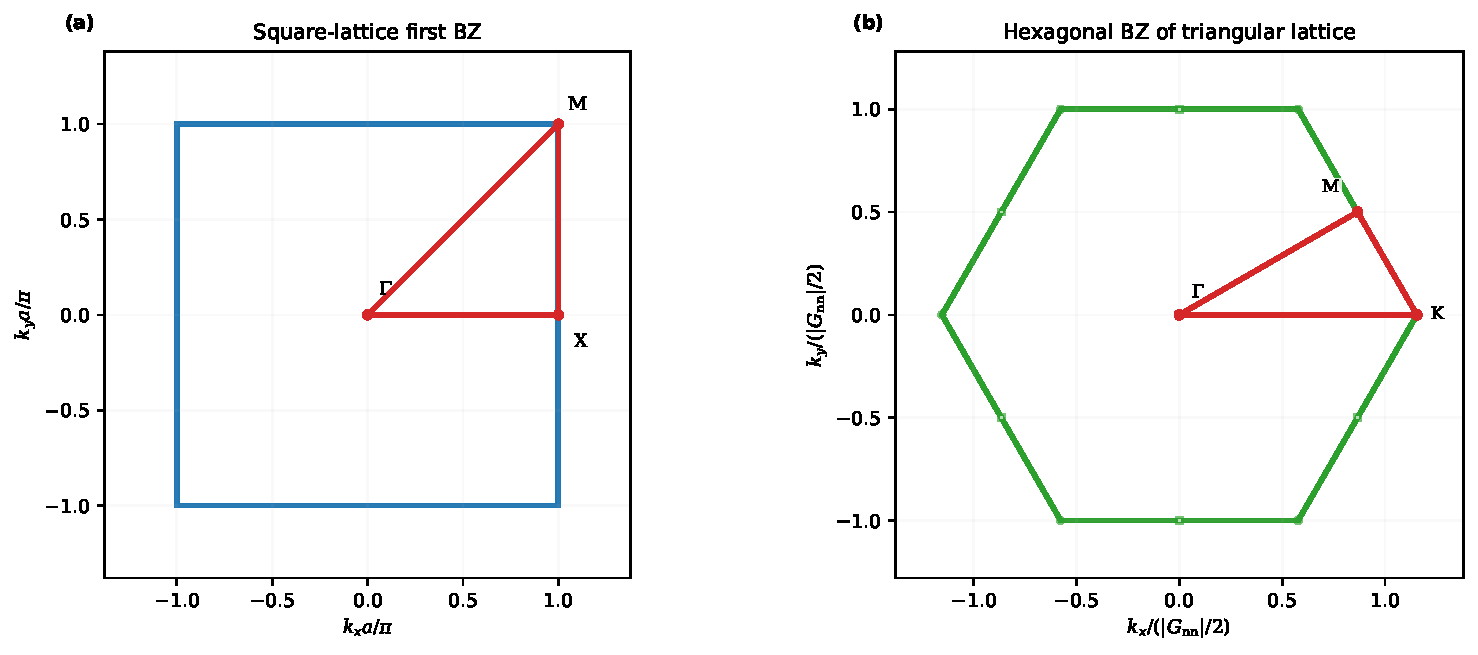
\includegraphics[width=0.94\linewidth]{fig_f3_reciprocal_lattice_bz.pdf}
 \caption{First Brillouin zones and standard high-symmetry paths in two
 common two-dimensional lattices. (a) For the square lattice the axes are
 $k_x a/\pi$ and $k_y a/\pi$; the first BZ is the square
 $[-1,1]^2$, and the red path is $\Gamma$--$X$--$M$--$\Gamma$.
 (b) For the triangular lattice the first BZ is hexagonal. The axes are
 normalized by $|G_{\mathrm{nn}}|/2$, where $G_{\mathrm{nn}}$ is a nearest
 reciprocal-lattice vector. In this convention the $K$-type points are
 the hexagon corners at radius $2/\sqrt{3}$, the $M$-type points are edge
 midpoints at radius $1$, and the red curve shows one
 $\Gamma$--$M$--$K$--$\Gamma$ sector. The two panels therefore use their
 natural reciprocal-space normalizations rather than a common length scale.}
 \label{fig:ch3-reciprocal-lattice-bz}
\end{figure}

Because $\epsr(\rr)$ is periodic, it admits a Fourier expansion:
\begin{equation}
 \epsr(\rr) = \sum_{\GG} \hat{\eps}_{\GG}\,e^{i\GG\cdot\rr},
 \label{eq:fourier-eps}
\end{equation}
where the sum runs over all reciprocal-lattice vectors and the Fourier
coefficients are
\begin{equation}
 \hat{\eps}_{\GG}
 = \frac{1}{|\Omega_{\mathrm{uc}}|}
 \int_{\Omega_{\mathrm{uc}}} \epsr(\rr)\,e^{-i\GG\cdot\rr}\;\dd^2 r.
 \label{eq:fourier-coeffs}
\end{equation}
The reality of $\epsr$ implies
$\hat{\eps}_{-\GG} = \hat{\eps}_{\GG}^*$.

\subsection{The dielectric scaling law}
\label{ssec:dielectric-scaling}

The Maxwell eigenproblem possesses a scaling property with no counterpart
in the Schr\"odinger equation. If $\epsr(\rr)$ describes a photonic crystal
with lattice constant~$a$, then the rescaled medium
$\epsr'(\rr) = \epsr(\rr/s)$ with lattice constant~$sa$ has eigenfrequencies
$\omega_n'(\kk') = \omega_n(\kk)/s$ at wave vectors $\kk' = \kk/s$.
The band structure scales inversely with the lattice constant, with no
change in shape:
\begin{equation}
 \frac{\omega_n(\kk)\,a}{2\pi c}
 = \frac{\omega_n'(\kk')\,(sa)}{2\pi c}.
 \label{eq:dielectric-scaling}
\end{equation}
This follows because the curl operator $\nabla\times$ scales as $1/a$
and the eigenvalue $\omega^2/c^2$ scales as $1/a^2$, while $\epsr$ is
dimensionless and unchanged by the spatial rescaling.

The scaling law has two practical consequences. First, band diagrams
are conventionally plotted in dimensionless units: the frequency axis is
$\omega a/(2\pi c)$ and the wave-vector axis is $ka/\pi$.
A single dimensionless band diagram then covers all physical lattice
constants simultaneously. Second, a photonic crystal designed at microwave
frequencies can be scaled to the optical regime simply by shrinking the
lattice constant, provided the material dispersion of $\epsr$ at the new
frequency is accounted for. This scale-free property is unique to
Maxwell's equations: the Schr\"odinger equation possesses a fundamental
length (the Bohr radius) set by $\hbar$, $m$, and $e$, so electronic
band structures do not rescale in this way.

The dimensionless presentation also clarifies the role of the dielectric
contrast $\varepsilon_{\max}/\varepsilon_{\min}$: it is the only
parameter (together with the geometry) that controls the dimensionless
band structure. Increasing the contrast widens all gaps simultaneously,
while changing the lattice constant merely shifts the physical frequency
scale.


%% ================================================================
\section{Bloch's theorem for Maxwell fields}
\label{sec:bloch-theorem}

The Maxwell curl--curl operator $\Mop$ defined in~\eqref{eq:maxwell-op-H}
commutes with the discrete translation operator
$T_{\mathbf{R}}\HH(\rr) = \HH(\rr + \mathbf{R})$, because
$\epsr(\rr + \mathbf{R}) = \epsr(\rr)$. Since $\Mop$ and
$\{T_{\mathbf{R}}\}$ share a common set of eigenstates, the eigenmodes of
$\Mop$ can be chosen to be simultaneous eigenstates of all lattice
translations:
\begin{equation}
 T_{\mathbf{R}}\,\HH_{n\kk}(\rr)
 = e^{i\kk\cdot\mathbf{R}}\,\HH_{n\kk}(\rr).
 \label{eq:bloch-condition}
\end{equation}
This is \emph{Bloch's theorem}. It states that each eigenmode can be
written as
\begin{equation}
 \boxed{
 \HH_{n\kk}(\rr) = e^{i\kk\cdot\rr}\,\mathbf{u}_{n\kk}(\rr),
 }
 \label{eq:bloch-mode}
\end{equation}
where $\mathbf{u}_{n\kk}(\rr)$ is a vector function with the periodicity
of the lattice: $\mathbf{u}_{n\kk}(\rr + \mathbf{R}) = \mathbf{u}_{n\kk}(\rr)$.

The band index $n = 1, 2, 3, \ldots$ labels the discrete eigenvalues at each
$\kk$, and $\kk$ is a continuous label running over the first Brillouin zone.
The eigenfrequency $\omega_n(\kk)$ as a function of $\kk$ is the
\emph{$n$-th photonic band}.

\begin{booknote}[Bloch's theorem is a consequence of symmetry]
The derivation above used only two ingredients: (i)~the operator $\Mop$
commutes with discrete translations, and (ii)~the translation operators
form an abelian group whose irreducible representations are one-dimensional
and labeled by $\kk$. No specific form of $\epsr$ was assumed beyond
periodicity. This means Bloch's theorem holds equally for the $\EE$-field
formulation, for magnetic media, and---crucially for later chapters---for
complex $\epsr$, as long as the periodicity is maintained. In the
non-Hermitian case, Bloch's theorem still provides a labeling by $\kk$,
but the eigenfrequencies become complex and the orthogonality of Bloch
modes fails.
\end{booknote}


%% ================================================================
\section{The unit-cell eigenproblem}
\label{sec:unit-cell}

Substituting the Bloch form~\eqref{eq:bloch-mode} into the Maxwell
eigenproblem $\Mop\HH = (\omega^2/c^2)\HH$ transforms the problem on
all of space into a problem on a single unit cell. Define the
$\kk$-dependent operator
\begin{equation}
 \Mop_\kk\,\mathbf{u}
 = (\nabla + i\kk)\times
 \left[\frac{1}{\epsr(\rr)}
 (\nabla + i\kk)\times\mathbf{u}\right],
 \label{eq:theta-k}
\end{equation}
which acts on periodic vector fields $\mathbf{u}(\rr)$ defined on
$\Omega_{\mathrm{uc}}$ with periodic boundary conditions. The eigenvalue
equation becomes
\begin{equation}
 \Mop_\kk\,\mathbf{u}_{n\kk}
 = \frac{\omega_n(\kk)^2}{c^2}\,\mathbf{u}_{n\kk},
 \label{eq:unit-cell-evp}
\end{equation}
with $\mathbf{u}_{n\kk}$ subject to periodic boundary conditions on
$\partial\Omega_{\mathrm{uc}}$.

The operator $\Mop_\kk$ is self-adjoint on the unit cell for real
$\epsr > 0$, because the surface terms from integration by parts cancel
between opposite faces (the Bloch phase factors have been absorbed into
$\nabla + i\kk$, and the boundary conditions are now strictly periodic).
Consequently, for each $\kk$ the eigenvalues
$\omega_n(\kk)^2/c^2$ are real and non-negative, the eigenfunctions
$\mathbf{u}_{n\kk}$ are orthogonal, and all the results of
Chapter~\ref{ch:energy-inner} apply with $\Mop$ replaced by $\Mop_\kk$.

The unit-cell eigenproblem~\eqref{eq:unit-cell-evp} is the starting point
for all numerical photonic band calculations. The standard approach
is to expand $\mathbf{u}_{n\kk}$ and $\epsr^{-1}$ in plane waves
(reciprocal-lattice vectors $\GG$), converting the differential equation
into a matrix eigenvalue problem that is solved for each $\kk$ on a
discrete grid in the Brillouin zone~\cite{paz2019tutorial}.


%% ================================================================
\section{One-dimensional photonic crystals}
\label{sec:1d-photonic-crystal}

Before treating two-dimensional systems, it is instructive to solve the
simplest photonic crystal exactly: a one-dimensional stack of alternating
dielectric layers. This example makes band gaps, Bloch wave vectors, and
the connection between the Maxwell eigenproblem and scattering theory
completely explicit.

\subsection{Transfer matrix for a bilayer}
\label{ssec:bilayer-transfer-ch3}

Consider a periodic stack along~$x$ with unit cell consisting of a layer
of thickness~$d_A$ and refractive index $n_A = \sqrt{\varepsilon_A}$
followed by a layer of thickness~$d_B$ and refractive index
$n_B = \sqrt{\varepsilon_B}$, so the period is $a = d_A + d_B$.
For normal incidence, the tangential field vector may be written as
$(E,\eta_0 H)^\transpose$, where the magnetic field is scaled by the
vacuum impedance. Its value at one side of the unit cell is related to
the value at the other side by a $2\times 2$ characteristic matrix~$M$:
\begin{equation}
 \begin{pmatrix} E_{m+1} \\ \eta_0 H_{m+1} \end{pmatrix}
 = M \begin{pmatrix} E_m \\ \eta_0 H_m \end{pmatrix},
 \qquad
 M = M_B \, M_A,
 \label{eq:1d-transfer}
\end{equation}
where the single-layer transfer matrix is
\begin{equation}
 M_j = \begin{pmatrix}
 \cos\phi_j & -i\sin\phi_j / n_j \\
 -i\,n_j\sin\phi_j & \cos\phi_j
 \end{pmatrix},
 \qquad
 \phi_j = \frac{\omega\,n_j\,d_j}{c},
 \label{eq:single-layer-transfer}
\end{equation}
for $j = A, B$. The phase $\phi_j$ is the optical path length through
layer~$j$ measured in radians. This transfer matrix is unimodular,
$\det M_j = 1$, as required by energy conservation in a lossless medium.
The product $M = M_B\,M_A$ is therefore also unimodular.

\subsection{Bloch condition and the dispersion relation}
\label{ssec:1d-dispersion}

Bloch's theorem requires that traversing one period multiplies the field
amplitudes by $e^{iKa}$, where $K$ is the Bloch wave vector. This means
$M$ has eigenvalue $e^{iKa}$, so
\begin{equation}
 \boxed{
 \cos(Ka) = \tfrac{1}{2}\operatorname{tr} M
 = \cos\phi_A\cos\phi_B
 - \tfrac{1}{2}\!\left(\frac{n_A}{n_B} + \frac{n_B}{n_A}\right)
 \sin\phi_A\sin\phi_B.
 }
 \label{eq:1d-dispersion-ch3}
\end{equation}
This is the exact photonic dispersion relation for a 1D periodic stack.
When $|\tfrac{1}{2}\operatorname{tr} M| \le 1$, the Bloch wave vector
$K$ is real and a propagating Bloch mode exists: these frequencies lie
in a \emph{pass band}. When $|\tfrac{1}{2}\operatorname{tr} M| > 1$,
$K$ acquires an imaginary part and the wave is evanescent: these
frequencies lie in a \emph{stop band} or band gap.

It is convenient to define the \emph{half-trace}
\begin{equation}
 \xi(\omega) \;\equiv\; \tfrac{1}{2}\operatorname{tr}M(\omega),
 \label{eq:half-trace-def}
\end{equation}
so that the pass-band condition is simply $|\xi|\le 1$.
The band structure is found by solving
$K(\omega) = \arccos[\xi(\omega)]/a$.
The result is a set of bands separated by gaps, plotted as $\omega$ versus
$K$ or equivalently as $K$ versus~$\omega$. When the two materials become
identical ($n_A = n_B$), the trace reduces to
$\cos(\omega a\,n/c)$ and the bands become the free-photon dispersion
folded into the first Brillouin zone, with no gaps.

The same trace formula is shown in Figure~\ref{fig:ch3-1d-transfer-bands}
for a representative high-contrast bilayer. This figure is deliberately
plotted in two equivalent ways: as pass bands in the reduced zone and as the
half-trace criterion. It is the inequality $|\xi(\omega)|\leq 1$, not the
visual shading, that defines a propagating Bloch wave.

\begin{figure}[t]
 \centering
 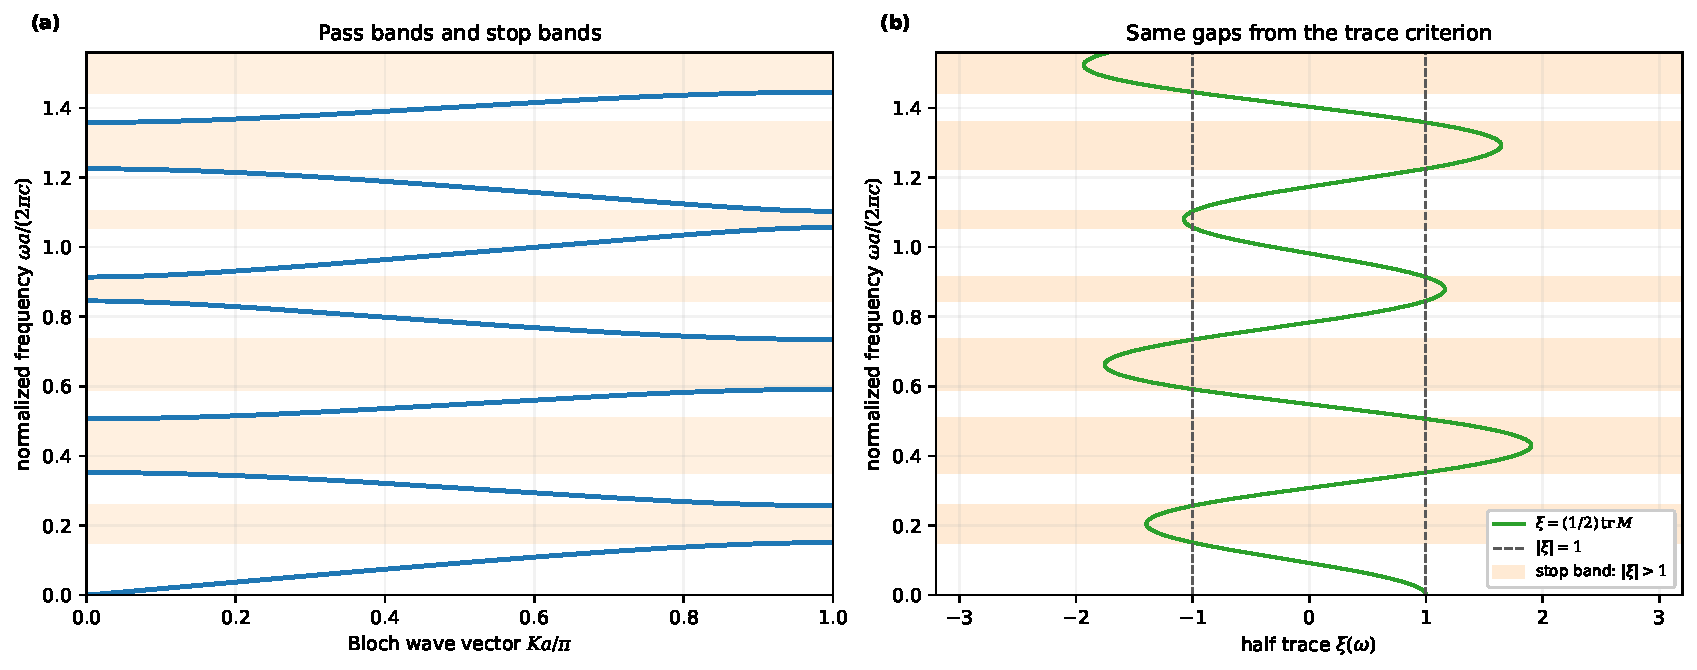
\includegraphics[width=0.94\linewidth]{fig_f3_1d_transfer_matrix_bands.pdf}
 \caption{Transfer-matrix view of one-dimensional photonic bands. The
 bilayer calculation uses $n_A=3.6$, $n_B=1$, and equal layer thicknesses
 $d_A=d_B=a/2$. (a) Blue curves show pass bands in which the Bloch wave
 vector $K$ is real. Orange intervals are stop bands. (b) The same
 information is encoded by the half trace
 $\xi(\omega)=\tfrac{1}{2}\operatorname{tr}M$: pass bands satisfy
 $|\xi|\leq 1$, while stop bands satisfy $|\xi|>1$. Every plotted
 pass-band point satisfies $|\xi|\leq 1$ to numerical precision.}
 \label{fig:ch3-1d-transfer-bands}
\end{figure}

\begin{example}[Quarter-wave stack]
\label{ex:quarter-wave}
The most important special case is the quarter-wave stack, in which each
layer has the same optical thickness:
$n_A d_A = n_B d_B = \lambda_B/4$, where $\lambda_B$ is the Bragg
wavelength. At the Bragg frequency $\omega_B = \pi c/(n_A d_A)$, both
phases equal $\pi/2$, the half-trace becomes
$\xi = -(n_A/n_B + n_B/n_A)/2$,
and the gap is widest. The fractional gap width (gap--midgap ratio) is
\begin{equation}
 \frac{\Delta\omega}{\omega_B}
 = \frac{4}{\pi}\arcsin\!\left(\frac{|n_A - n_B|}{n_A + n_B}\right),
 \label{eq:gap-midgap}
\end{equation}
which grows monotonically with the refractive-index contrast. For
a quarter-wave stack with $\varepsilon_A = 13$ ($n_A = \sqrt{13} \approx 3.61$)
and $\varepsilon_B = 1$ ($n_B = 1$),
Eq.~\eqref{eq:gap-midgap} gives a fundamental gap--midgap ratio of
approximately $77\%$---an exceptionally wide gap reflecting the large
contrast. (For the equal-thickness bilayer of
Figure~\ref{fig:ch3-1d-transfer-bands}, which does not satisfy the
quarter-wave condition, the first gap--midgap ratio is smaller, about $52\%$.)
\end{example}

\subsection{Connection to the scattering matrix}
\label{ssec:1d-smatrix}

The transfer matrix of $N$ unit cells is $M^N$. Using the Cayley--Hamilton
theorem for a unimodular $2\times 2$ matrix, $M^N$ can be expressed in
terms of Chebyshev polynomials of the second kind:
\begin{equation}
 M^N = U_{N-1}(\xi)\,M - U_{N-2}(\xi)\,I,
 \qquad \xi = \tfrac{1}{2}\operatorname{tr}M,
 \label{eq:chebyshev-transfer}
\end{equation}
where $U_m(\xi) = \sin[(m+1)\arccos\xi]/\sin[\arccos\xi]$. In a pass
band ($|\xi| \le 1$), the finite-stack transmission exhibits $N - 1$
Fabry--P\'erot oscillations between successive gap edges. In a stop band
($|\xi| > 1$), $U_{N-1}$ grows exponentially with~$N$, and the
transmission decays as $e^{-2\,\mathrm{Im}(K)\,Na}$. This connects the
Bloch band structure directly to the poles and zeros of the scattering
matrix discussed in Chapter~\ref{ch:poles-zeros}: each pass-band
resonance of the finite stack is a precursor of a Bloch band, and the
stop band corresponds to a frequency window where no S-matrix pole
approaches the real axis.

The 1D transfer-matrix approach extends naturally to complex~$\epsr$
(Chapters~\ref{ch:loss-gain-dispersion} and~\ref{ch:pt-symmetric}), where the Bloch
wave vector becomes complex even inside pass bands, and the sharp
distinction between pass and stop bands blurs into a continuous complex
band structure (Chapter~\ref{ch:complex-bands}).


%% ================================================================
\section{Band structure in two dimensions}
\label{sec:2d-bands}

In a two-dimensional photonic crystal with $\epsr(x,y)$ periodic in the
$(x,y)$ plane, $\mur = 1$, and fields independent of $z$ (or at fixed
$k_z = 0$), the vector Maxwell eigenproblem decouples into the two scalar
polarizations introduced in Section~\ref{sec:2d-reductions}.

\subsection{TM bands}
\label{ssec:tm-bands}

For TM polarization ($\EE = E_z\hat{z}$), the Bloch form is
$E_{z,n\kk}(\rr) = e^{i\kk\cdot\rr}\,\phi_{n\kk}(\rr)$ with
$\phi_{n\kk}$ periodic. The unit-cell eigenproblem becomes
\begin{equation}
 -(\nabla_\perp + i\kk)^2\,\phi_{n\kk}(\rr)
 = \frac{\omega_n(\kk)^2}{c^2}\,\epsr(\rr)\,\phi_{n\kk}(\rr).
 \label{eq:tm-bloch}
\end{equation}
The eigenvalue is $\omega_n^2/c^2$ and the weight on the right is
$\epsr(\rr)$, so the inner product is the $\epsr$-weighted one
from~\eqref{eq:tm-inner}.

\subsection{TE bands}
\label{ssec:te-bands}

For TE polarization ($\HH = H_z\hat{z}$), the Bloch form is
$H_{z,n\kk}(\rr) = e^{i\kk\cdot\rr}\,\psi_{n\kk}(\rr)$ with
$\psi_{n\kk}$ periodic. The unit-cell eigenproblem is
\begin{equation}
 -(\nabla_\perp + i\kk)\cdot
 \left[\frac{1}{\epsr(\rr)}\,
 (\nabla_\perp + i\kk)\,\psi_{n\kk}(\rr)\right]
 = \frac{\omega_n(\kk)^2}{c^2}\,\psi_{n\kk}(\rr).
 \label{eq:te-bloch}
\end{equation}
Here the weight is unity and the inner product is the unweighted one
from~\eqref{eq:te-inner}.

\begin{remark}
The TM and TE band structures can be very different for the same lattice,
because the spatial structure of the operator differs: TM modes ``see''
$\epsr$ as a multiplicative weight, while TE modes ``see''
$\epsr^{-1}$ inside a divergence operator. A complete photonic band
gap---a frequency range forbidden to \emph{both} polarizations---requires
the TM and TE gaps to overlap, which imposes strong constraints on the
lattice geometry and dielectric contrast.
\end{remark}


\subsection{The plane-wave expansion method}
\label{ssec:pwe}

The standard numerical approach to the unit-cell eigenproblem~\eqref{eq:unit-cell-evp} is the
\emph{plane-wave expansion} (PWE) method~\cite{wu2015scheme,hsu2016bound}. Expand the periodic part of
the Bloch mode in reciprocal-lattice vectors:
\begin{equation}
 \mathbf{u}_{n\kk}(\rr)
 = \sum_{\GG} \tilde{\mathbf{u}}_{n\kk}(\GG)\,e^{i\GG\cdot\rr}.
 \label{eq:pwe-expansion}
\end{equation}
Substituting into~\eqref{eq:unit-cell-evp} and projecting onto each
$\GG'$ yields a matrix eigenvalue problem. For TM polarization in 2D,
where $E_z$ is a scalar, the equation~\eqref{eq:tm-bloch} gives the
generalized eigenvalue problem
\begin{equation}
 |\kk + \GG'|^2\,
 \tilde{\phi}_{n\kk}(\GG')
 =
 \frac{\omega_n(\kk)^2}{c^2}
 \sum_{\GG}
 \hat{\varepsilon}_{\GG'-\GG}\,
 \tilde{\phi}_{n\kk}(\GG),
 \label{eq:pwe-tm}
\end{equation}
where $\hat{\varepsilon}_{\GG'-\GG}$ is the Fourier coefficient of
$\epsr(\rr)$ at reciprocal-lattice vector $\GG' - \GG$. This is a
Hermitian generalized eigenvalue problem of size $N_G \times N_G$, where
$N_G$ is the number of plane waves retained. For TE polarization, by
contrast, the Fourier coefficients of $\epsr^{-1}$ enter the operator
side, reflecting the weighted Laplacian in~\eqref{eq:te-bloch}.

Convergence is algebraic in $N_G$: smooth $\epsr$ profiles converge
rapidly, while sharp interfaces converge more slowly due to the Gibbs
phenomenon in the Fourier representation of discontinuous material
profiles.
Improved formulations such as the Ho--Chan--Soukoulis inverse rule treat
the discontinuity correctly by applying the appropriate Fourier
factorization rule to normal and tangential field components, significantly
improving convergence for high-contrast structures~\cite{paz2019tutorial}.

For the full vector problem in 3D, the expansion must enforce the
transversality constraint $(\kk + \GG)\cdot\tilde{\mathbf{u}} = 0$ for
each plane wave, reducing the degrees of freedom from three to two
per~$\GG$. The resulting Hermitian matrix eigenvalue problem is larger
but structurally similar.

\begin{example}[2D rod array: square lattice]
\label{ex:2d-rod}
Consider a square array (period~$a$) of circular dielectric rods
($\varepsilon_{\mathrm{rod}} = 8.9$, radius $r = 0.2a$) in air
($\varepsilon_{\mathrm{bg}} = 1$). The filling fraction is
$f = \pi r^2/a^2 \approx 0.126$. A plane-wave expansion with
$N_G \approx 500$ converges the lowest six TM bands to four significant
figures. The TM band structure shows a large gap between the first and
second bands (gap--midgap ratio $\approx 37\%$), while the TE bands have
no complete gap at this filling fraction. This asymmetry between TM and
TE gaps is generic for rod-in-air geometries and can be understood from
the field-concentration argument of the next section.
\end{example}

\begin{figure}[t]
 \centering
 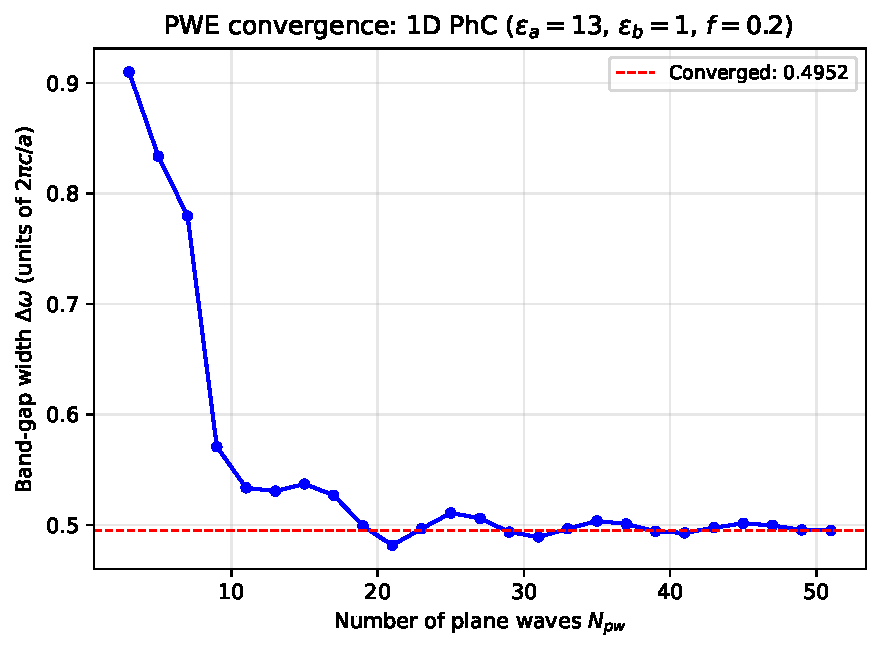
\includegraphics[width=0.6\linewidth]{figures/fig_f03_pwe_convergence.pdf}
 \caption{Convergence of the plane-wave expansion for a 1D photonic
 crystal ($\varepsilon_a = 13$, $\varepsilon_b = 1$, filling fraction
 $f = 0.2$). The computed band-gap width converges rapidly with the
 number of plane waves $N_{\mathrm{pw}}$, reaching the converged value
 $\Delta\omega \approx 0.495$ (in units of $2\pi c/a$) for
 $N_{\mathrm{pw}} \gtrsim 30$ in this one-dimensional test. In higher
 dimensions, sharp high-contrast interfaces usually require more careful
 Fourier factorization and significantly more plane waves.}
 \label{fig:pwe-convergence}
\end{figure}


%% ================================================================
\section{Band gaps}
\label{sec:band-gaps}

A \emph{photonic band gap} is a frequency interval
$[\omega_{\mathrm{low}}, \omega_{\mathrm{high}}]$ in which no Bloch mode
exists for any $\kk$ in the Brillouin zone. The physical consequence is
that light at frequencies within the gap cannot propagate through the
crystal: it is exponentially attenuated, decaying as
$e^{-\kappa(\omega)\,x}$ with a penetration depth set by the imaginary
wave vector $\kappa$.

The existence of a gap requires sufficient dielectric contrast
$\varepsilon_{\max}/\varepsilon_{\min}$ and appropriate lattice geometry. For TM
modes in a 2D crystal of high-$\epsr$ rods in air, gaps open readily;
for TE modes, connected high-$\epsr$ regions (such as air holes in a
dielectric slab) are more favorable.

\paragraph{Perturbative origin of gaps.}
At a Brillouin-zone boundary or high-symmetry point, two bands that would
cross in a uniform medium are coupled by the periodic modulation of
$\epsr$. The resulting level repulsion opens a gap whose width, to
first order in the Fourier coefficient $\hat{\eps}_{\GG}$ of the
relevant reciprocal-lattice vector, is proportional to
$|\hat{\eps}_{\GG}|$. This is the photonic analogue of the
nearly-free-electron picture in solid-state physics.

\paragraph{Variational bounds.}
Since $\Mop_\kk$ is self-adjoint, the Rayleigh quotient provides
variational bounds on the band-edge frequencies. The lowest band satisfies
\begin{equation}
 \frac{\omega_1(\kk)^2}{c^2}
 \le \frac{\int_{\Omega_{\mathrm{uc}}}
 \epsr^{-1}\,|(\nabla + i\kk)\times\mathbf{u}|^2\;\dd^2 r}
 {\int_{\Omega_{\mathrm{uc}}} |\mathbf{u}|^2\;\dd^2 r}
 \label{eq:variational-band}
\end{equation}
for any trial function $\mathbf{u}$, with equality when $\mathbf{u}$
is the exact Bloch eigenfunction. Higher bands are bounded by the
min--max principle. These variational estimates are the theoretical
foundation of the plane-wave expansion method.


\subsection{Field concentration and the physical origin of gaps}
\label{ssec:field-concentration}

The variational principle provides a remarkably intuitive explanation for
why gaps open and which polarization is favored. Consider the two
band-edge modes at a Brillouin-zone boundary where a gap opens. One
mode---the \emph{dielectric band} or lower band edge---concentrates its
electric-field energy in the high-$\epsr$ regions, while the other---the
\emph{air band} or upper band edge---concentrates its energy in the
low-$\epsr$ regions.

The dielectric-band mode has a lower eigenfrequency because the Rayleigh
quotient~\eqref{eq:variational-band} involves $\epsr^{-1}$ in the
numerator: concentrating $|\nabla\times\mathbf{u}|^2$ where $\epsr^{-1}$
is small (i.e., where $\epsr$ is large) reduces the numerator and hence
the eigenvalue. Conversely, the air-band mode is forced to have its curl
energy where $\epsr^{-1}$ is large, raising the eigenvalue. The frequency
difference between these two modes is the band gap.

This field-concentration mechanism explains the TM/TE asymmetry observed
in the 2D example above:
\begin{itemize}
\item \emph{TM modes in rod arrays.} The $E_z$ field is a scalar and
 can concentrate efficiently inside isolated high-$\epsr$ rods. The
 dielectric and air bands have very different field distributions,
 producing a large gap.
\item \emph{TE modes in rod arrays.} The in-plane $\HH$ field must
 satisfy continuity conditions at the rod boundaries that prevent it
 from concentrating entirely inside the rods. The dielectric and air
 bands are more similar, and the gap is small or absent.
\item \emph{TE modes in hole arrays.} When the high-$\epsr$ region is
 connected (air holes in a dielectric slab), the in-plane $\HH$ field
 \emph{can} concentrate in the connected dielectric, and TE gaps open
 readily.
\end{itemize}
A complete photonic band gap---forbidden to both polarizations---therefore
requires a geometry that simultaneously favors both TM and TE gaps, such
as a triangular lattice of air holes with appropriately chosen radius and
dielectric contrast.

The field-concentration picture also explains why gap width increases
with dielectric contrast: larger contrast amplifies the frequency
splitting between modes that concentrate in different materials. This is
precisely the effect captured by the Fourier coefficient
$|\hat{\eps}_{\GG}|$ in the perturbative estimate, which itself grows
with contrast.


%% ================================================================
\section{Degeneracies and symmetry}
\label{sec:degeneracies}

At generic points in the Brillouin zone, the eigenvalues $\omega_n(\kk)$
are non-degenerate. Degeneracies can occur at high-symmetry points where
the little group (the subgroup of the point group that leaves $\kk$
invariant) has irreducible representations of dimension greater than one.

\subsection{Dirac points}
\label{ssec:dirac}

At the $K$ and $K'$ points of a hexagonal Brillouin zone, a pair of bands
may touch linearly, forming a \emph{Dirac cone}~\cite{haldane2008possible,rechtsman2013photonic,khanikaev2013photonic}:
\begin{equation}
 \omega_\pm(\kk) \approx \omega_D \pm v_D\,|\kk - \kk_D| + \cdots,
 \label{eq:dirac-cone}
\end{equation}
where $\omega_D$ is the Dirac frequency and $v_D$ is an effective group
velocity. Near a Dirac point, the two-band effective Hamiltonian takes
the form
\begin{equation}
 H_{\mathrm{eff}}(\delta\kk)
 = v_D\bigl(\delta k_x\,\sigma_x + \delta k_y\,\sigma_y\bigr),
 \label{eq:dirac-hamiltonian}
\end{equation}
with $\sigma_{x,y}$ the Pauli matrices acting on the two-band subspace.
This is the photonic analogue of graphene's electronic Dirac cone.

\subsection{Quadratic touchings and accidental degeneracies}
\label{ssec:quadratic}

At the $\Gamma$ point, symmetry can enforce a quadratic band touching
where $\omega(\kk) \propto |\kk|^2$ rather than $|\kk|$. Perturbations
that break the protecting symmetry can open a gap or split the touching
into a pair of Dirac points.

Accidental degeneracies---those not enforced by symmetry---are generically
avoided in a two-parameter family (the two components of $\kk$ in 2D).
However, they can be tuned by adjusting a third parameter (e.g., the
rod radius or the dielectric contrast). When two bands approach each
other and reconnect, the topology of the band structure can change.


%% ================================================================
\section{Orthogonality and normalization of Bloch modes}
\label{sec:bloch-orthogonality}

The Bloch modes satisfy orthogonality relations that follow from the
self-adjointness of $\Mop_\kk$. For two modes at the \emph{same}
$\kk$,
\begin{equation}
 \int_{\Omega_{\mathrm{uc}}}
 \mathbf{u}_{m\kk}^*(\rr)\cdot\mathbf{u}_{n\kk}(\rr)\;\dd^2 r
 = \delta_{mn},
 \label{eq:bloch-ortho}
\end{equation}
after normalization. For modes at \emph{different} $\kk$ and $\kk'$, the
full Bloch modes $\HH_{n\kk}$ and $\HH_{m\kk'}$ are orthogonal over all
space (or, equivalently, their overlap per unit cell vanishes when
$\kk \neq \kk'$).

This orthonormality is the basis for expanding arbitrary fields in Bloch
modes, defining projection operators onto individual bands, and---as we
shall see in Chapter~\ref{ch:berry-maxwell}---computing the Berry
connection and curvature from the $\kk$-dependence of $\mathbf{u}_{n\kk}$.


%% ================================================================
\section{Group velocity, effective mass, and density of states}
\label{sec:group-velocity-dos}

Beyond the eigenfrequencies $\omega_n(\kk)$, the dispersion surface
contains essential physical information through its derivatives.

\subsection{Group velocity}
\label{ssec:group-velocity}

The group velocity of a Bloch mode is the gradient of the dispersion
relation:
\begin{equation}
 \mathbf{v}_g = \nabla_\kk\,\omega_n(\kk).
 \label{eq:group-velocity}
\end{equation}
It can also be expressed as an expectation value using the
Hellmann--Feynman theorem. Differentiating the unit-cell
eigenproblem~\eqref{eq:unit-cell-evp} with respect to~$\kk$ gives
\begin{equation}
 \mathbf{v}_g
 = \frac{c^2}{2\omega_n}
 \frac{\displaystyle
 \int_{\Omega_{\mathrm{uc}}}
 \mathbf{u}_{n\kk}^*\cdot
 \bigl[
 (\nabla_\kk\Mop_\kk)\,\mathbf{u}_{n\kk}
 \bigr]\;\dd^2 r}
 {\displaystyle
 \int_{\Omega_{\mathrm{uc}}}
 |\mathbf{u}_{n\kk}|^2\;\dd^2 r},
 \label{eq:hellmann-feynman-vg}
\end{equation}
where $\nabla_\kk\Mop_\kk$ is obtained by differentiating the
operator $(\nabla + i\kk)\times[\epsr^{-1}(\nabla + i\kk)\times\,\cdot]$
with respect to~$\kk$. This expression guarantees that the group velocity
is real and bounded whenever $\Mop_\kk$ is self-adjoint.
In non-Hermitian systems, the self-adjointness fails and the group velocity
becomes complex; the physical interpretation of wave-packet propagation
must then be revisited (Chapter~\ref{ch:complex-bands}).

\subsection{Effective mass at band edges}
\label{ssec:effective-mass}

At band edges, where $\nabla_\kk\omega_n = 0$, the band curvature defines
an effective inverse-mass tensor:
\begin{equation}
 (m^{-1})_{ij}
 = \frac{\partial^2\omega_n}{\partial k_i\,\partial k_j}
 \bigg|_{\kk = \kk_0}.
 \label{eq:effective-mass}
\end{equation}
Near a band edge at $\kk_0$, the dispersion is parabolic:
$\omega_n(\kk) \approx \omega_n(\kk_0) + \tfrac{1}{2}\sum_{ij}
(m^{-1})_{ij}\,\delta k_i\,\delta k_j$. This effective-mass
approximation is the photonic analogue of the semiconductor effective mass
and forms the basis for envelope-function theories of photonic-crystal
defect modes and waveguides: a defect introduced into the crystal acts as
a potential well in the envelope equation, binding states pulled out of
the adjacent band edge into the gap.

The effective mass also controls the curvature of the equifrequency
contour near the band edge. An isotropic parabolic band has circular
contours; an anisotropic band has elliptical contours whose principal axes
are aligned with the eigenvectors of $(m^{-1})_{ij}$. In self-collimation
effects, the equifrequency contour is made flat over a range of~$\kk$,
so that wave packets propagate with nearly zero angular spread despite
the discrete lattice.

\subsection{Density of states and van Hove singularities}
\label{ssec:dos}

The \emph{photonic density of states} (DOS) counts the number of modes
per unit frequency. For a two-dimensional photonic crystal,
\begin{equation}
 \rho(\omega)
 = \sum_n \int_{\mathrm{BZ}}
 \delta\bigl(\omega - \omega_n(\kk)\bigr)\;
 \frac{\dd^2 k}{(2\pi)^2}.
 \label{eq:dos}
\end{equation}
(In three dimensions the integration measure becomes
$\dd^3 k/(2\pi)^3$.)
Inside a band gap, $\rho(\omega) = 0$: there are no propagating modes.
This is precisely why spontaneous emission is inhibited in a photonic
band-gap material---the emitter simply has no modes into which it can
radiate.

At band edges, the vanishing group velocity produces \emph{van Hove
singularities} in the DOS. In two dimensions, these are logarithmic
divergences; in three dimensions, they manifest as square-root edges.
Physically, the diverging DOS means that a large number of modes are
compressed into a narrow frequency range, which strongly enhances
light--matter interaction. Slow-light devices, enhanced nonlinear optics,
and low-threshold lasing in photonic crystals all exploit the high DOS
near band edges.

Figure~\ref{fig:ch3-group-velocity-dos} shows the same idea in a simple
model where the geometry is visible at a glance. It is not meant to be a
full plane-wave calculation for a particular dielectric pattern; it is a
teaching model for how stationary points of a dispersion surface become
features of the DOS.

\begin{figure}[t]
 \centering
 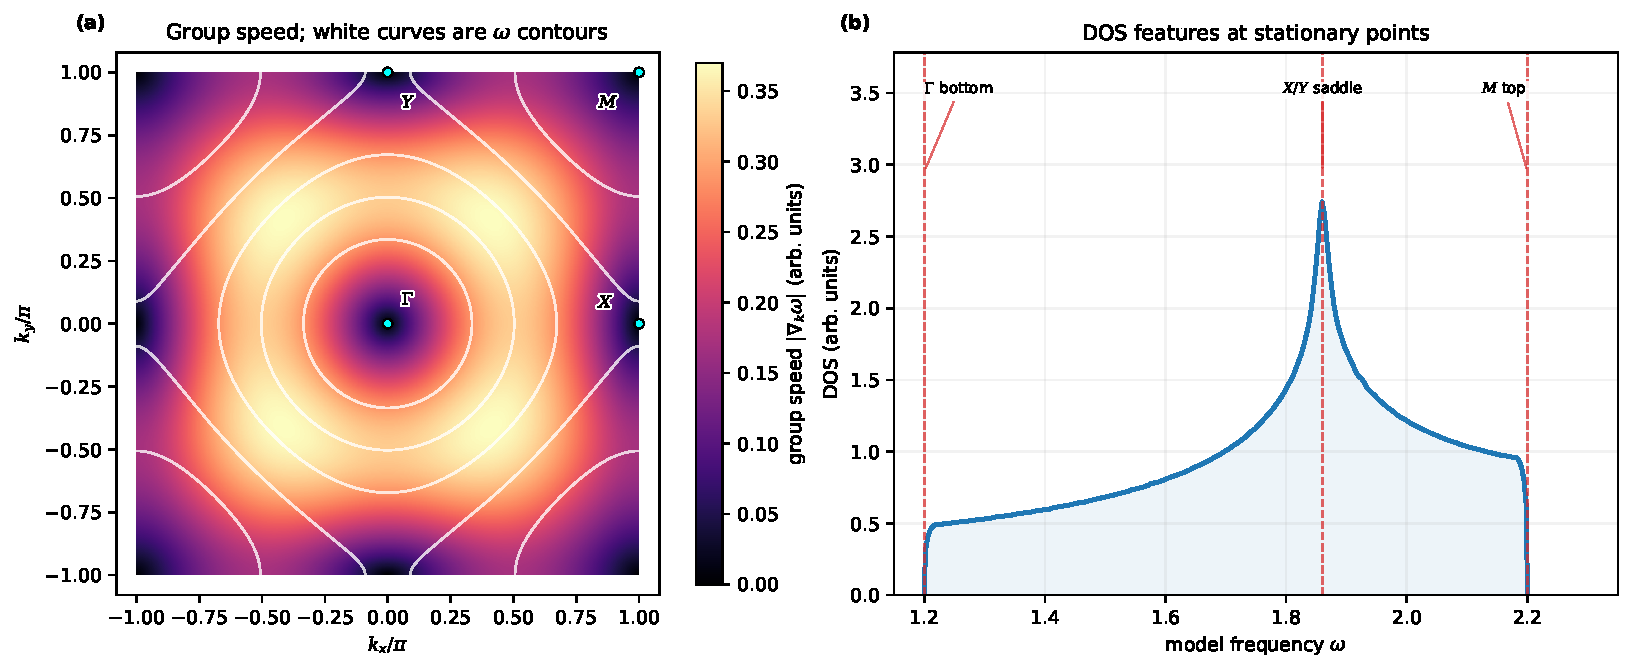
\includegraphics[width=0.94\linewidth]{fig_f3_group_velocity_dos.pdf}
 \caption{Group velocity and density of states in a pedagogical
 square-lattice band model. (a) The colour shows
 $|\nabla_{\kk}\omega|$ and the white curves are constant-frequency
 contours. Stationary points occur at $\Gamma$, at the symmetry-related
 $X/Y$ saddle points, and at $M$. (b) A histogram-smoothed, model-normalized
 DOS in arbitrary units. The dashed lines mark the corresponding band
 bottom, van-Hove saddle feature, and band top. In a full Maxwell band
 calculation the same relation is expressed by
 Eq.~\eqref{eq:dos}: DOS features arise where the dispersion surface has
 small or vanishing group velocity.}
 \label{fig:ch3-group-velocity-dos}
\end{figure}

The local density of states (LDOS), introduced in
Chapter~\ref{ch:light-eigenvalue}, is the position-resolved version of
$\rho(\omega)$ and determines the Purcell enhancement of a dipole emitter
at a given location in the crystal. In the Hermitian case, the LDOS is
non-negative and can be computed from the Bloch-mode expansion. In
non-Hermitian systems (Chapter~\ref{ch:qnm}), the LDOS
must instead be reconstructed from quasinormal modes or from the full
Green tensor. Individual modal contributions can have signs and phases
that have no Hermitian analogue, so only the properly assembled physical
response has the usual positivity properties in passive systems.

\begin{takeaway}[From band diagrams to physical observables]
The photonic band structure is not just a plot---it encodes group
velocity, effective mass, density of states, and through these, the
propagation, confinement, emission, and interaction of light in the
crystal. Every derivative of $\omega_n(\kk)$ carries physical meaning,
and every singularity of the band structure controls a physical effect.
\end{takeaway}


%% ================================================================
\section{Beyond Hermitian bands: a preview}
\label{sec:nh-preview}

The entire construction of this chapter assumed real, positive $\epsr$.
What happens when this assumption is relaxed?

\paragraph{Complex permittivity.}
If $\epsr(\rr) = \epsr'(\rr) + i\epsr''(\rr)$ with the same spatial
periodicity, Bloch's theorem still holds---it depends only on discrete
translational symmetry, not on Hermiticity. But the eigenfrequencies
$\omega_n(\kk)$ become complex, the bands lift off the real axis into the
complex frequency plane, and the orthogonality~\eqref{eq:bloch-ortho}
fails. The ``band structure'' becomes a set of complex-valued curves
$\omega_n(\kk)$, and new topological invariants---winding numbers in the
complex frequency plane---replace the familiar Chern numbers. This is
the subject of Chapters~\ref{ch:complex-bands} and~\ref{ch:point-gap}.

\paragraph{Non-reciprocal media.}
If the permittivity tensor $\epsr(\rr)$ is not symmetric (as in a
magneto-optical medium), time-reversal symmetry is broken and the band
structure loses the constraint $\omega_n(\kk) = \omega_n(-\kk)$. Gaps
can carry nonzero Chern numbers, and topologically protected one-way edge
states appear. This is the domain of topological photonics~\cite{ozawa2018topological,hafezi2013imaging,l2014topological}, developed in
Chapter~\ref{ch:berry-maxwell}.

\paragraph{Open or finite crystals.}
A photonic crystal of finite extent has no exact translational symmetry.
Bloch's theorem does not apply, and the spectrum changes from continuous
bands to a discrete set of resonances. In Hermitian systems, the
bulk-boundary correspondence connects the band topology to the existence
of edge states. In non-Hermitian systems, this correspondence can fail
through the skin effect
(Chapter~\ref{ch:skin-effect}).

\begin{takeaway}[Photonic bands as the Hermitian foundation]
The band structure $\omega_n(\kk)$ of a lossless periodic photonic crystal,
derived from the self-adjoint Maxwell operator acting on Bloch modes in a
unit cell, provides the Hermitian foundation on which all non-Hermitian
photonic band theory is built. Real eigenfrequencies, orthogonal Bloch
modes, variational bounds, and well-defined band gaps are the standard
from which complex bands, point-gap topology, and the skin effect depart.
\end{takeaway}

\chapter{Boundaries, Radiation, and Scattering}
\label{ch:boundaries}

\begin{chapterlead}
Chapters~\ref{ch:light-eigenvalue}--\ref{ch:periodicity} established the
spectral theory of closed or periodic photonic systems, where the
operator $\Mop$ is self-adjoint and the eigenfrequencies are real.
Real photonic structures, however, are rarely closed. Light escapes:
a microcavity leaks, a nanoparticle radiates, a grating diffracts.
The moment we impose outgoing-wave boundary conditions to describe this
radiation, the mathematical framework changes qualitatively.
Eigenfrequencies become complex, modes cease to be normalizable in the
usual sense, and the scattering matrix---with its poles and
zeros---replaces the eigenvalue spectrum as the central object.
The scattering framework developed below connects the Hermitian
foundations of Part~I to the non-Hermitian physics of Part~II.
\end{chapterlead}


%% ================================================================
\section{From cavities to open systems}
\label{sec:open-systems}

A perfectly closed cavity---surrounded by perfect electric conductors
(PEC)---supports a discrete, real spectrum as shown in
Section~\ref{sec:spectrum-types}. No energy leaves or enters the cavity,
and the modes are orthogonal standing waves.

Now remove one mirror, or replace the PEC walls with a finite dielectric
boundary. Energy can escape. A mode that was perfectly trapped at
frequency $\omega_0$ now decays in time at a rate $\gamma$, and the
effective eigenfrequency becomes complex:
\begin{equation}
 \omtil_n = \omega_n - i\gamma_n, \qquad \gamma_n > 0.
 \label{eq:complex-freq}
\end{equation}
The field oscillates at $\omega_n$ and decays as $e^{-\gamma_n t}$.
The quality factor is $\Qfac_n = \omega_n / (2\gamma_n)$: higher $\Qfac$
means slower leakage.

This has mathematical consequences. The complex frequency
signals a fundamental change in the mathematical structure of the
Maxwell eigenproblem. Outgoing-wave boundary conditions render the
operator non-self-adjoint, and the entire machinery of Hermitian spectral
theory---real eigenvalues, orthogonality, completeness, energy inner
product---must be rebuilt. That reconstruction is the subject of
Chapter~\ref{ch:qnm}; here we set the stage by introducing the
scattering matrix and the role of boundary conditions.

\subsection{Energy balance in open systems}
\label{ssec:energy-balance-open}

For a finite region $\Omega$ surrounding the scatterer, the time-averaged
Poynting balance can be written as
\begin{equation}
 -\dv{U}{t}
 = P_{\mathrm{rad}} + P_{\mathrm{abs}},
 \qquad
 P_{\mathrm{rad}}
 = \oint_{\partial\Omega}\langle\mathbf{S}\rangle\cdot\nn\;\dd S,
 \label{eq:poynting-open}
\end{equation}
where $U=\int_\Omega \langle u\rangle\,\dd^3 r$ is the stored
electromagnetic energy and $P_{\mathrm{abs}}$ is the power absorbed by
the material inside $\Omega$. For a closed cavity with PEC walls,
$P_{\mathrm{rad}}=0$ and energy is conserved (or dissipated only by
material absorption). For an open system, $P_{\mathrm{rad}}>0$ represents
power carried away by outgoing waves. This radiation loss is irreversible
in the reduced cavity description and is the physical origin of the
imaginary part of the eigenfrequency.

The energy decay rate of a mode with complex frequency
$\omtil = \omega - i\gamma$ is $2\gamma$, and the time-averaged stored
energy $U$ and radiated power $P_{\mathrm{rad}}$ are related by
\begin{equation}
 \Qfac = \omega\,\frac{U}{P_{\mathrm{rad}} + P_{\mathrm{abs}}}
 = \frac{\omega}{2\gamma}.
 \label{eq:Q-from-power}
\end{equation}
When material absorption is negligible, $\Qfac$ is determined solely by
the radiation loss, which is controlled by the geometry of the cavity
opening and the refractive-index contrast at the boundary.


%% ================================================================
\section{Outgoing-wave boundary conditions}
\label{sec:outgoing-bc}

\subsection{The Silver--M\"uller radiation condition}
\label{ssec:silver-muller}

In an open system, we require that far from the scatterer the
electromagnetic field consist only of outgoing waves. In three
dimensions, this is the \emph{Silver--M\"uller radiation condition}:
\begin{equation}
 \lim_{r\to\infty}\left[
 r\left(\sqrt{\muvac}\,\HH\times\hat{\rr}
 - \sqrt{\epsvac}\,\EE\right)
 \right] = 0,
 \label{eq:silver-muller}
\end{equation}
uniformly in angle. The factor is $r$ in three dimensions because
outgoing spherical waves decay as $1/r$; in two-dimensional cylindrical
problems the corresponding condition uses the $\sqrt{r}$ asymptotic
factor. In one dimension, it reduces to requiring a purely outgoing
traveling wave $e^{+ikr}$ (with our $e^{-i\omega t}$ convention) at large
distances.

The Silver--M\"uller condition is the electromagnetic analogue of the
Sommerfeld radiation condition for scalar waves. It ensures that the
scattered field represents power flowing away from the scatterer,
not toward it---a physical requirement for any passive, causal system.

\subsection{Why outgoing-wave conditions break self-adjointness}
\label{ssec:outgoing-breaks-sa}

Unlike the PEC condition $\nn\times\EE = 0$, the outgoing-wave condition
does not make the surface term in the self-adjointness
proof~\eqref{eq:surface-vanish} vanish. Instead, the outgoing wave carries a
nonzero Poynting flux through any enclosing surface:
\begin{equation}
 \oint_{\partial\Omega}\langle\mathbf{S}\rangle\cdot\nn\;\dd S
 = P_{\mathrm{rad}} > 0.
 \label{eq:radiated-power}
\end{equation}
This radiation loss is the physical mechanism by which openness destroys
self-adjointness. Formally, if we try to verify
$\langle\mathbf{F},\Mop\mathbf{G}\rangle
= \langle\Mop\mathbf{F},\mathbf{G}\rangle$ for two outgoing-wave
solutions, the surface integral~\eqref{eq:surface-vanish} leaves a nonzero
remainder proportional to the cross-flux between $\mathbf{F}$ and
$\mathbf{G}$.

The failure of self-adjointness is not a technicality---it is the
mathematical expression of a deep physical fact: an open system exchanges
energy with its environment, and the environment's degrees of freedom are
not included in the operator $\Mop$. The full system (scatterer plus
radiation field at infinity) is still governed by the self-adjoint Maxwell
operator on all of space, but the reduced description restricted to
the scatterer alone is non-self-adjoint. This is the first instance of
a theme that will recur throughout the book: non-Hermiticity as the price
of a reduced description.

\begin{remark}
The outgoing-wave boundary condition depends on frequency through the
wave vector $k = \omega/c$. This means the eigenproblem is nonlinear in
$\omega$: we cannot simply write $\Mop\HH = \omega^2\HH$ with a fixed
$\Mop$ independent of $\omega$. Instead, for each candidate complex
$\omtil$, the boundary condition changes. This is why the eigenfrequencies
of open systems are called \emph{resonances} rather than eigenvalues in the
strict sense.
\end{remark}


%% ================================================================
\section{The scattering matrix}
\label{sec:smatrix}

\subsection{Definition and physical meaning}
\label{ssec:smatrix-def}

Consider a scatterer illuminated by an incoming wave. The total field is
$\EE = \EE_{\mathrm{in}} + \EE_{\mathrm{sc}}$, where $\EE_{\mathrm{sc}}$
satisfies the outgoing-wave condition. If the scatterer is linear, the
relation between incoming and outgoing wave amplitudes defines the
\emph{scattering matrix} $\Smat(\omega)$.

For a one-dimensional layered structure with waves incident from the left
and right, the $2\times 2$ scattering matrix relates incoming amplitudes
$(a_L^+, a_R^-)$ to outgoing amplitudes $(a_L^-, a_R^+)$:
\begin{equation}
 \begin{pmatrix} a_L^- \\ a_R^+ \end{pmatrix}
 = \Smat(\omega)
 \begin{pmatrix} a_L^+ \\ a_R^- \end{pmatrix}
 = \begin{pmatrix} r_L & t' \\ t & r_R \end{pmatrix}
 \begin{pmatrix} a_L^+ \\ a_R^- \end{pmatrix},
 \label{eq:smatrix-1d}
\end{equation}
where $r_L$, $r_R$ are the reflection coefficients from the left and right,
and $t$, $t'$ are the transmission coefficients. For a reciprocal medium,
$t = t'$; for a $\PT$-symmetric structure, additional constraints apply
(Chapter~\ref{ch:pt-symmetric}).

For a general three-dimensional scatterer with $N$ incoming and outgoing
channels (propagating modes of the surrounding medium), $\Smat$ is an
$N\times N$ matrix. The channels may be angular-momentum partial waves
(for spherical scatterers), waveguide modes (for integrated photonic
circuits), or diffraction orders (for periodic gratings).

The physical content of $\Smat(\omega)$ is a complete input-output
description of the scatterer: given any incident field (decomposed into
channel amplitudes), $\Smat$ determines the scattered field. All
measurable quantities---reflection, transmission, absorption,
scattering cross-sections---can be extracted from $\Smat$.

\begin{figure}[t]
 \centering
 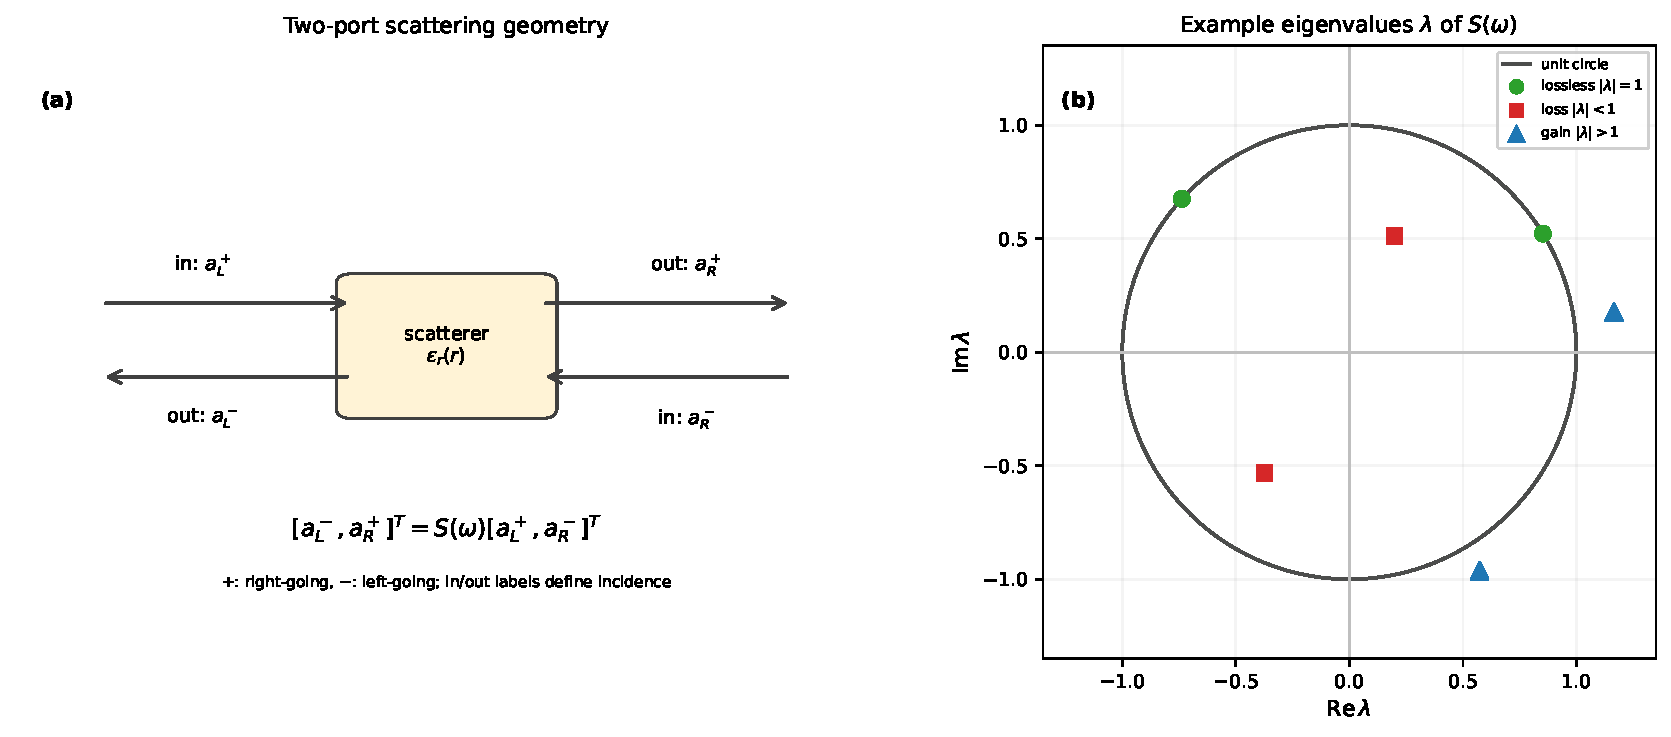
\includegraphics[width=0.98\textwidth]{fig_f4_scattering_channels.pdf}
 \caption{The scattering matrix as an input--output map. Panel (a) defines the two-channel amplitudes used in Eq.~\eqref{eq:smatrix-1d}. Panel (b) shows the corresponding constraint on scattering eigenvalues: lossless systems place them on the unit circle, passive loss moves them inside, and gain can move them outside. This is the scattering version of the distinction between Hermitian and non-Hermitian Maxwell operators.}
 \label{fig:ch4-scattering-channels}
\end{figure}

\subsection{Unitarity and energy conservation}
\label{ssec:unitarity}

For a lossless scatterer (real $\epsr$ everywhere), conservation of the
time-averaged Poynting flux demands that $\Smat$ be unitary:
\begin{equation}
 \Smat^\adj\,\Smat = \mathbf{I}.
 \label{eq:unitarity}
\end{equation}
This is the scattering-matrix analogue of the self-adjointness of $\Mop$.
Unitarity means that the total outgoing power equals the total incoming
power: no energy is created or destroyed inside the scatterer.

For a scatterer with loss, unitarity is violated in a specific direction:
\begin{equation}
 \Smat^\adj\Smat \le \mathbf{I}
 \qquad (\text{sub-unitary: lossy}),
 \label{eq:sub-unitary}
\end{equation}
meaning the eigenvalues of $\Smat^\adj\Smat$ are all $\le 1$. The
deficit represents absorbed power. For a scatterer with gain,
$\Smat^\adj\Smat$ can have eigenvalues $> 1$: the scatterer amplifies
the incident field. The transition from sub-unitary to super-unitary
$\Smat$ as gain is increased corresponds to the transition from a passive
absorber to an active amplifier, and eventually to a laser when a pole
of $\Smat$ reaches the real frequency axis.

\subsection{Reciprocity in scattering}
\label{ssec:smatrix-reciprocity}

For a reciprocal medium (symmetric $\epsr$ tensor), the scattering matrix
satisfies the symmetry
\begin{equation}
 \Smat^\transpose = \Smat,
 \label{eq:smatrix-reciprocal}
\end{equation}
after appropriate normalization of the channel amplitudes. As discussed in
Section~\ref{sec:reciprocity}, reciprocity is distinct from unitarity
(Hermiticity of the Hamiltonian). A lossy reciprocal scatterer has
$\Smat^\transpose = \Smat$ but $\Smat^\adj\Smat \neq \mathbf{I}$.

The distinction is important because it constrains which non-Hermitian
effects are possible in reciprocal media. For example, reciprocity
guarantees $t_L = t_R$ (equal transmission from both sides), even when the
system has gain and loss that break unitarity and produce
$r_L \neq r_R$ (unequal reflection). The directional reflection asymmetry
exploited by $\PT$-symmetric devices (Chapter~\ref{ch:pt-symmetric}) is
therefore consistent with reciprocity.

\subsection{The optical theorem}
\label{ssec:optical-theorem}

For a single incoming channel, the total scattering cross-section
$\sigma_{\mathrm{sc}}$ and the extinction cross-section
$\sigma_{\mathrm{ext}}$ are related by the optical theorem:
\begin{equation}
 \sigma_{\mathrm{ext}} = \frac{4\pi}{k}\,\Im\!\bigl[f(0)\bigr],
 \label{eq:optical-theorem}
\end{equation}
where $f(0)$ is the forward scattering amplitude and $k = \omega/c$.
Extinction equals the sum of scattering and absorption:
$\sigma_{\mathrm{ext}} = \sigma_{\mathrm{sc}} + \sigma_{\mathrm{abs}}$.
For a passive, lossless scatterer, $\sigma_{\mathrm{abs}} = 0$ and
extinction is purely due to scattering.

The optical theorem is a consequence of unitarity and can be derived
directly from the $\Smat$-matrix formalism. It fails for active
(amplifying) scatterers, where $\sigma_{\mathrm{ext}}$ can become
negative---the scattered field interferes constructively with the incident
field in the forward direction, \emph{increasing} the total power. This
is a scattering-theory signature of gain.


%% ================================================================
\section{Poles, zeros, and resonances}
\label{sec:poles-zeros-ch4}

The scattering matrix $\Smat(\omega)$ is a meromorphic function of the
complex frequency $\omega$. Its singularity structure encodes the
complete physics of the open system.

\subsection{Poles: resonances and quasinormal modes}
\label{ssec:poles}

A \emph{pole} of $\Smat(\omega)$ is a complex frequency $\omtil_n$ at
which the scattering matrix diverges. Physically, this means a nonzero
outgoing field exists with no incoming field---the system radiates
spontaneously. The poles are the resonances (quasinormal-mode
frequencies) of the open system~\cite{vial2014quasimodal}.

For a passive system with no gain, all poles lie in the lower half of
the complex $\omega$ plane ($\Im\omtil < 0$), corresponding to decaying
modes. A pole on the real axis would represent a mode with infinite
lifetime---a bound state or, in special circumstances, a bound state in
the continuum (Chapter~\ref{ch:bic-topology}).

Near a single isolated pole, the scattering matrix has the form
\begin{equation}
 \Smat(\omega) \approx \Smat_{\mathrm{bg}}
 + \frac{\mathbf{A}_n}{\omega - \omtil_n},
 \label{eq:pole-expansion}
\end{equation}
where $\Smat_{\mathrm{bg}}$ is a slowly varying background and
$\mathbf{A}_n$ is the residue matrix, whose rank equals the multiplicity
of the pole. This Breit--Wigner form~\cite{alpeggiani2017quasinormal,sauvan2014modal,lasson2014roundtrip} is the foundation of temporal
coupled-mode theory (Chapter~\ref{ch:maxwell-coupled-modes}).

\subsection{Zeros: coherent perfect absorption}
\label{ssec:zeros}

A \emph{zero} of $\Smat(\omega)$---more precisely, a zero of
$\det\Smat(\omega)$---is a frequency at which a specific combination of
incoming waves produces zero outgoing field. All incident energy is
absorbed. This is \emph{coherent perfect absorption} (CPA)~\cite{sweeney2019perfectly,wang2021coherent}, the
time-reverse of lasing. The interplay of poles and zeros under
$\PT$ symmetry is the subject of Chapter~\ref{ch:poles-zeros}.

For a two-channel system, a zero of $\det\Smat$ requires both the
absorption condition ($\Im\varepsilon > 0$) and the correct phase
relationship between the two input beams. The CPA condition is thus
doubly constrained---in both frequency and input-phase space---making it
more experimentally demanding than simple absorption.

\subsection{Pole--zero structure and causality}
\label{ssec:pole-zero-causality}

Causality constrains the analytic structure of $\Smat(\omega)$: in the
upper half of the complex $\omega$ plane ($\Im\omega > 0$), $\Smat$ must
be analytic and bounded for a passive system. Poles can only appear in
the lower half-plane. If gain is introduced, poles can migrate upward;
when a pole crosses the real axis, the system reaches the lasing
threshold.

The zeros of $\det\Smat$ for a passive system lie in the upper
half-plane (by the time-reversal argument: if the poles of
$\Smat$ are in the lower half-plane, the poles of
$\Smat^{-1}$---which are the zeros of $\det\Smat$---are in the
upper half-plane for a time-reversal-symmetric system). This
pole-zero separation is the scattering-theory version of passivity~\cite{zhao2019connection}.
Chapter~\ref{ch:poles-zeros} shows how gain brings poles and zeros
together, culminating in the CPA-laser point where a pole and a zero
meet on the real axis.


%% ================================================================
\section{The Fabry--P\'erot resonator}
\label{sec:fabry-perot}

The simplest and most instructive open resonator is a one-dimensional
Fabry--P\'erot cavity: two partial mirrors separated by a distance $L$
filled with a medium of refractive index $n$. Despite its simplicity, the
Fabry--P\'erot cavity contains, in miniature, all the essential features of
open-system scattering: complex eigenfrequencies, a meromorphic $\Smat$,
and a connection between poles and transmission resonances.

\subsection{Transfer matrix and scattering matrix}
\label{ssec:fp-transfer}

Each mirror is characterized by reflection and transmission coefficients
$r_j$, $t_j$ ($j = 1,2$). The \emph{transfer matrix} $\Tmat$ relates
the field amplitudes on the left to those on the right through
\begin{equation}
 \Tmat = \Tmat_{\mathrm{mirror},1}\,\Tmat_{\mathrm{prop}}(L)\,
 \Tmat_{\mathrm{mirror},2},
 \label{eq:transfer-fp}
\end{equation}
where $\Tmat_{\mathrm{prop}}(L) = \bigl(\begin{smallmatrix} e^{in\omega L/c} & 0
\\ 0 & e^{-in\omega L/c}\end{smallmatrix}\bigr)$ accounts for propagation over
distance $L$ and each mirror matrix encodes the partial reflection and
transmission. The scattering matrix is obtained from $\Tmat$ by a
standard change of basis~(Appendix~\ref{app:transfer}).

For symmetric mirrors ($r_1 = r_2 = r$, $t_1 = t_2 = t$), the
transmission coefficient is
\begin{equation}
 t_{\mathrm{FP}}(\omega) = \frac{(1-|r|^2)\,e^{in\omega L/c}}
 {1 - r^2\,e^{2in\omega L/c}},
 \label{eq:fp-transmission-coeff}
\end{equation}
and the power transmission is the Airy function:
\begin{equation}
 T(\omega) = |t_{\mathrm{FP}}|^2
 = \frac{(1-|r|^2)^2}
 {1 - 2|r|^2\cos(2n\omega L/c) + |r|^4}
 = \frac{1}{1 + F\sin^2(n\omega L/c)},
 \label{eq:airy}
\end{equation}
where the \emph{coefficient of finesse} is
\begin{equation}
 F = \frac{4|r|^2}{(1-|r|^2)^2}.
 \label{eq:finesse-coeff}
\end{equation}
The finesse $\mathcal{F} = \pi\sqrt{F}/2 = \pi|r|/(1-|r|^2)$
measures the sharpness of the transmission peaks relative to the free
spectral range $\Delta\omega_{\mathrm{FSR}} = \pi c/(nL)$.

\subsection{Resonance condition and complex eigenfrequencies}
\label{ssec:resonance-condition}

The poles of the scattering matrix correspond to the condition
\begin{equation}
 r^2\,e^{2in\omtil L/c} = 1,
 \label{eq:fp-resonance}
\end{equation}
which has solutions at complex frequencies
\begin{equation}
 \omtil_m = \frac{m\pi c}{nL}
 - \frac{ic\ln(1/|r|^2)}{2nL},
 \qquad m = 1,2,3,\ldots
 \label{eq:fp-poles-boundaries}
\end{equation}
for real $r$ with $|r| < 1$. The real part gives equally
spaced resonant frequencies (the free spectral range), and the imaginary
part gives the decay rate $\gamma = c\ln(1/|r|)/(nL)$. The quality
factor is
\begin{equation}
 \Qfac_m = \frac{\omega_m}{2\gamma}
 = \frac{m\pi}{2\ln(1/|r|)}.
 \label{eq:fp-Q}
\end{equation}
Higher-order modes ($m \gg 1$) have higher $\Qfac$ because $\omega_m$
grows while $\gamma$ stays fixed. For high reflectivity ($|r| \to 1$),
$\gamma \to 0$ and $\Qfac \to \infty$: the cavity approaches the
closed-cavity limit, and the eigenfrequencies approach the real axis.

\paragraph{Example.}
A silicon slab in air with $n = 3.5$ and $L = 300\;\mathrm{nm}$ has
Fresnel reflectivity $|r| = |n-1|/(n+1) = 0.556$, giving
$\gamma \approx 1.68 \times 10^{14}\;\mathrm{rad/s}$ and
$\Qfac_1 \approx 2.67$. This very low quality factor reflects
the poor confinement of a bare dielectric slab.
Adding distributed Bragg reflectors increases $|r|$ and pushes the poles
closer to the real axis: the quasinormal-mode picture recovers smoothly
the transition from a leaky slab to a high-finesse cavity.
Chapter~\ref{ch:qnm} develops this example further and connects it to
the full QNM pole structure.

\begin{figure}[t]
 \centering
 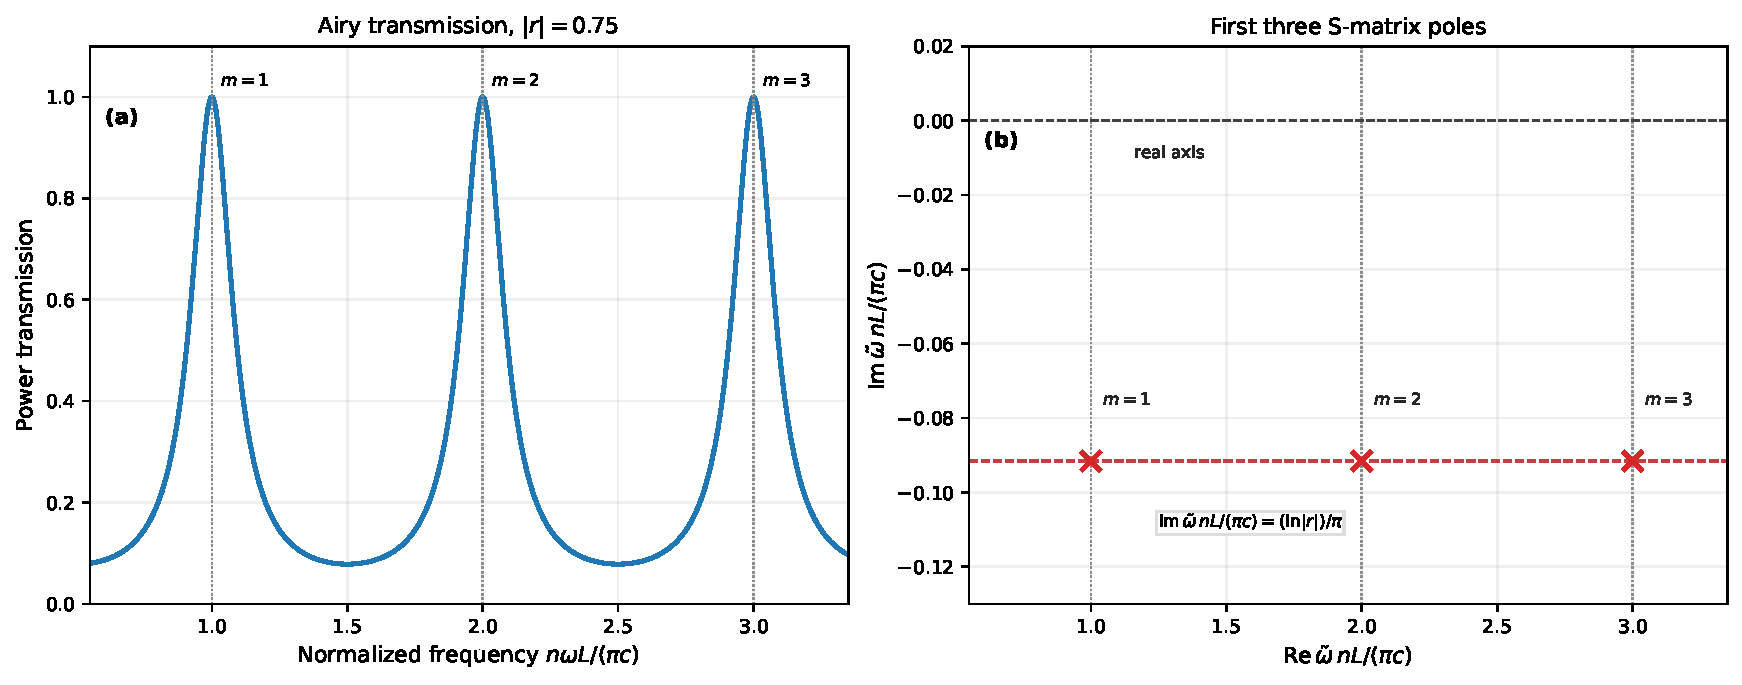
\includegraphics[width=0.98\textwidth]{fig_f4_fabry_perot_airy_poles.pdf}
 \caption{The same Fabry--P\'erot resonances seen on the real axis and in the complex plane. Panel (a) shows the Airy transmission peaks as a function of round-trip phase. Panel (b) shows the corresponding scattering poles: the real parts set the peak positions and the imaginary part sets the linewidth.}
 \label{fig:ch4-fabry-perot-airy-poles}
\end{figure}

\subsection{Connection between poles and transmission peaks}
\label{ssec:poles-transmission}

The transmission peaks of the Airy function~\eqref{eq:airy} occur at real
frequencies $\omega_m = m\pi c/(nL)$, which are the real parts of the
poles~\eqref{eq:fp-poles-boundaries}. The full width at half maximum
(FWHM) of each peak is $\delta\omega \approx 2\gamma$, which is twice
the imaginary part of the pole. Thus the poles of $\Smat$ directly
determine the observable transmission spectrum: their real parts give the
peak positions and their imaginary parts give the peak widths.

This connection between complex poles and real-frequency observables is
general: for any open resonator, the scattering spectrum near a resonance
is a Lorentzian (or Fano) line shape whose parameters are set by the
nearest pole of $\Smat$. The full scattering response is the
superposition of contributions from all poles, weighted by their residues
(the Mittag-Leffler expansion of Chapter~\ref{ch:poles-zeros}).

\begin{booknote}[The Fabry--P\'erot as a non-Hermitian paradigm]
The Fabry--P\'erot resonator is the simplest example of how openness
creates non-Hermiticity. The interior of the cavity is lossless (real
$n$), yet the eigenfrequencies are complex because energy leaks through
the partially reflecting mirrors. This is a concrete realization of the
second of the four roads to non-Hermiticity identified in
Section~\ref{ssec:three-conditions}: the boundary conditions, not the
material, break self-adjointness. The pole structure of $\Smat$
provides a complete description of the resonator's spectral response,
replacing the discrete real eigenvalues of a closed cavity with a
constellation of complex poles in the lower half-plane.
\end{booknote}


%% ================================================================
\section{Scattering cross-sections and the Wigner time delay}
\label{sec:cross-sections}

\subsection{Cross-sections from the $\Smat$ matrix}
\label{ssec:cross-from-s}

For a compact scatterer in free space, the total scattering cross-section
$\sigma_{\mathrm{sc}}$ and the absorption cross-section
$\sigma_{\mathrm{abs}}$ can be expressed in terms of the eigenvalues
$s_n(\omega)$ of the $\Smat$ matrix:
\begin{align}
 \sigma_{\mathrm{sc}} &= \frac{\pi}{k^2}\sum_n |1 - s_n|^2,
 \label{eq:sigma-sc}\\
 \sigma_{\mathrm{abs}} &= \frac{\pi}{k^2}\sum_n (1 - |s_n|^2).
 \label{eq:sigma-abs}
\end{align}
For a unitary $\Smat$, $|s_n| = 1$ and $\sigma_{\mathrm{abs}} = 0$: no
absorption occurs, as expected for a lossless scatterer.

The extinction cross-section is
$\sigma_{\mathrm{ext}} = \sigma_{\mathrm{sc}} + \sigma_{\mathrm{abs}}$,
and the optical theorem~\eqref{eq:optical-theorem} relates it to the
forward scattering amplitude. Near a resonance at $\omtil_n$, the
extinction cross-section exhibits a Lorentzian peak:
\begin{equation}
 \sigma_{\mathrm{ext}}(\omega) \approx \sigma_0
 \frac{\gamma_n^2}{(\omega - \omega_n)^2 + \gamma_n^2},
 \label{eq:resonant-extinction}
\end{equation}
where $\sigma_0$ is the peak cross-section, which can exceed the
geometric cross-section by a factor of order $\Qfac$.

\subsection{The Wigner time delay}
\label{ssec:wigner-delay}

The $\Smat$ matrix also characterizes the temporal response of the
scatterer through the Wigner--Smith time-delay matrix~\cite{raman2010photonic,unknown2018phys}:
\begin{equation}
 Q_{\mathrm{WS}} = -i\,\Smat^\adj\,\dv{\Smat}{\omega}.
 \label{eq:wigner-smith}
\end{equation}
For a unitary $\Smat$, $Q_{\mathrm{WS}}$ is Hermitian, and its
eigenvalues $\tau_n(\omega)$ are real time delays~\cite{lasson2014roundtrip}---the durations for
which an incoming wave packet is trapped inside the scatterer before
being released. Near a resonance, the dominant eigenvalue of
$Q_{\mathrm{WS}}$ is of order the resonance lifetime. With the convention
$\omtil_n=\omega_n-i\gamma_n$, the stored energy decays at rate
$2\gamma_n$, so the energy lifetime is
$\tau_E=1/(2\gamma_n)=\Qfac_n/\omega_n$. Phase-delay conventions can
differ by factors of order unity, but the scaling is the same:
high-$\Qfac$ resonances trap light for long times.

\begin{figure}[t]
 \centering
 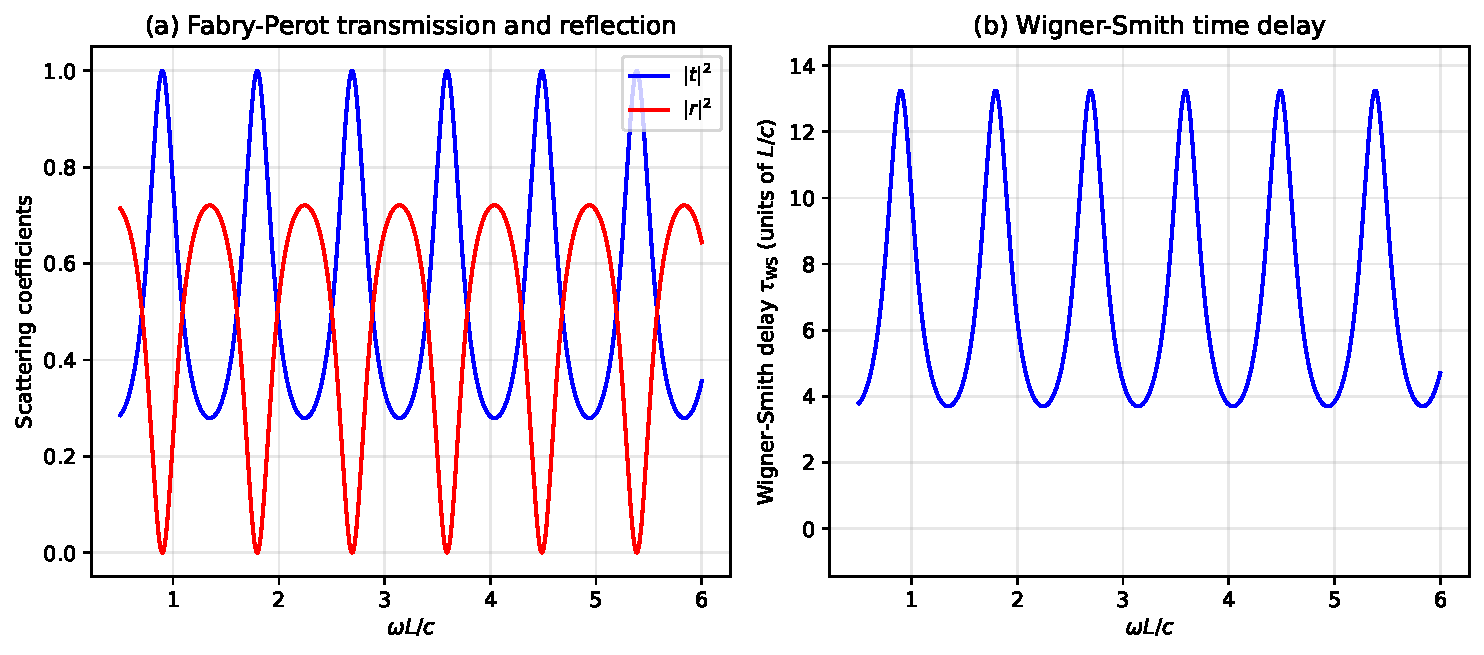
\includegraphics[width=0.85\linewidth]{figures/fig_f04_wigner_smith.pdf}
 \caption{Wigner--Smith time delay for a Fabry--P\'erot cavity
 ($n = 3.5$, $L = 1$).
 (a)~Transmission $|t|^2$ and reflection $|r|^2$ showing the
 characteristic resonance peaks of the etalon.
 (b)~The Wigner--Smith delay
 $\tau_{\mathrm{WS}} = \dd(\arg\det\Smat)/\dd\omega$ peaks sharply
 at each resonance, confirming that high-$\Qfac$ modes trap light for
 long times. Between resonances the delay is small, reflecting the
 short dwell time of off-resonant wave packets.}
 \label{fig:wigner-smith}
\end{figure}

When the $\Smat$ matrix is non-unitary (lossy or amplifying scatterer),
$Q_{\mathrm{WS}}$ is no longer Hermitian, and the time delays become
complex. The imaginary part of the time delay characterizes the
amplification or absorption experienced by the trapped wave packet.
This non-Hermitian time delay is an observable quantity that can be
measured interferometrically and provides a direct experimental
probe of the non-Hermitian character of the scattering process.


%% ================================================================
\section{Spectrum of the open Maxwell operator}
\label{sec:open-spectrum}

For a general open system---not just a Fabry--P\'erot cavity---the
spectrum of the Maxwell operator with outgoing boundary conditions has a
richer structure than the discrete, real spectrum of a closed
cavity~\cite{vial2014quasimodal}.

\paragraph{Discrete resonances.}
The complex eigenfrequencies $\omtil_n$ (poles of $\Smat$) form a
discrete set in the lower half of the complex $\omega$ plane. Near each
pole, the scattered field is dominated by the corresponding quasinormal
mode, whose spatial profile diverges exponentially at infinity (the mode
was excited in the past and its radiation wavefront keeps expanding).

\paragraph{Continuous spectrum.}
In addition to the discrete resonances, the open operator has a
\emph{continuous spectrum} on the real frequency axis, corresponding to
radiation modes that propagate freely in the surrounding medium. These
modes are not square-integrable and cannot be normalized in the same
Hilbert space as bound states.

\paragraph{Bound states and guided modes.}
If the scatterer supports guided modes or bound states (fields that decay
exponentially in all directions without radiation), these appear as
discrete, real eigenfrequencies. They coexist with the continuous
spectrum. In certain symmetry-protected situations, a discrete real
eigenvalue can be embedded \emph{within} the continuous spectrum---a
bound state in the continuum (Chapter~\ref{ch:bic-topology}).

\paragraph{Branch cuts.}
In the complex $\omega$ plane, the continuous spectrum produces branch
cuts rather than isolated singularities. The choice of branch cut
(typically along the negative imaginary axis or the real axis) determines
which Riemann sheet the resonance poles are defined on. This subtlety
becomes important for the mathematical theory of quasinormal-mode
completeness (Chapter~\ref{ch:qnm}).

The full spectral decomposition of the field in an open system requires
all three components: the discrete resonances, the continuous radiation
modes, and any bound states~\cite{vial2014quasimodal}. This is why the
modal theory of open photonic systems is fundamentally different from
that of closed cavities: the resonances alone do not form a complete
basis, and the standard orthogonality relations fail.

\begin{figure}[t]
 \centering
 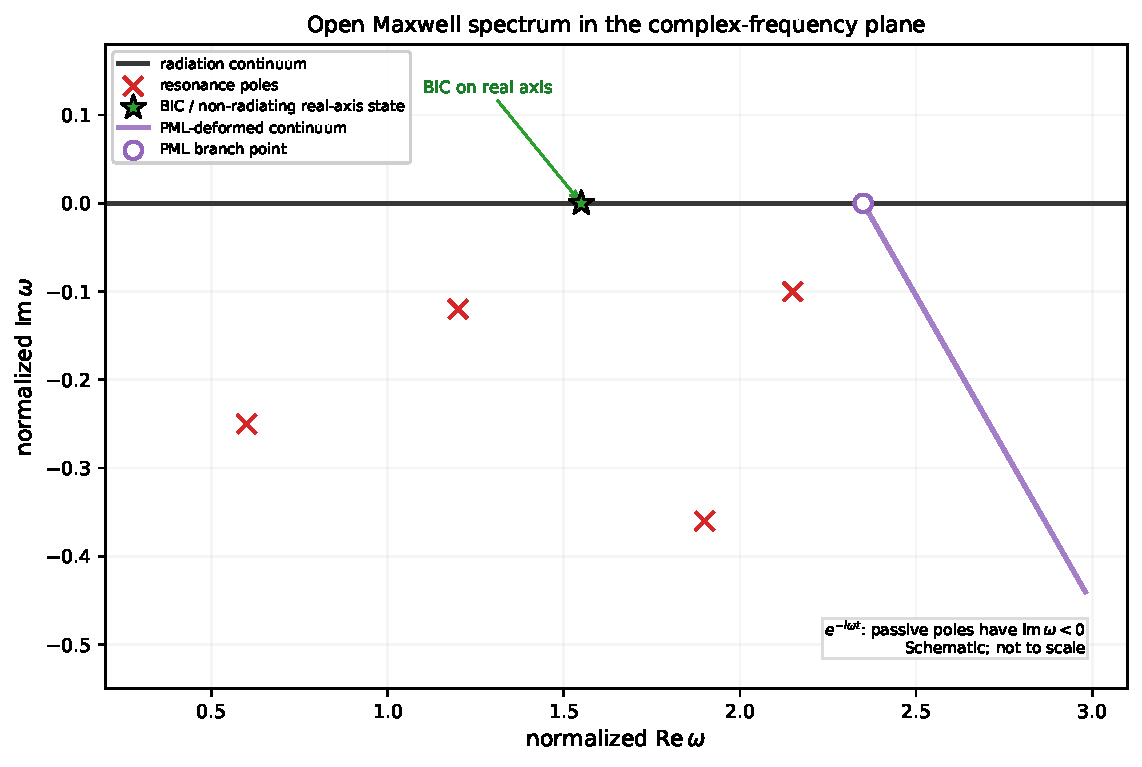
\includegraphics[width=0.88\textwidth]{fig_f4_complex_frequency_plane.pdf}
 \caption{Open-system spectra in the complex-frequency plane. Passive
 resonances appear as poles below the real axis; radiation modes form a
 continuum on the real axis; and a guided mode or BIC can remain on the
 real axis without radiating. In a complex-scaled or PML-truncated
 formulation, the radiation continuum is represented by a rotated or
 discretized set of PML modes in the lower half-plane. The marked point
 indicates a continuum threshold or branch point of the radiation channel,
 not an additional resonance of the scatterer. This picture anticipates
 the quasinormal-mode theory of Chapter~\ref{ch:qnm}.}
 \label{fig:ch4-complex-frequency-plane}
\end{figure}


%% ================================================================
\section{Perfectly matched layers}
\label{sec:pml}

\subsection{Complex coordinate stretching}
\label{ssec:pml-stretching}

Numerical computation of resonances requires truncating the infinite
domain to a finite computational region. Simply truncating creates
artificial reflections at the boundary. \emph{Perfectly matched layers}
(PMLs) solve this problem by introducing a complex coordinate
stretching in the outer region that absorbs outgoing waves without
reflection.

In one dimension, the PML replaces the physical coordinate $x$ with
\begin{equation}
 \tilde{x}(x) = x + \frac{i}{\omega}\int_0^x \sigma(x')\;\dd x',
 \label{eq:pml-stretch}
\end{equation}
where $\sigma(x) \ge 0$ is a smooth absorption profile that vanishes
inside the physical domain and grows in the PML region. A plane wave
$e^{ikx}$ in the physical region becomes
$e^{ik\tilde{x}} = e^{ikx}\,\exp\!\bigl(-k\int_0^x\sigma(x')\dd x'/\omega\bigr)$
in the PML region---exponentially decaying for outgoing waves ($k > 0$)
and exponentially growing for incoming waves ($k < 0$). Since only
outgoing waves are present (by the radiation condition), the PML absorbs
all radiation without reflection.

In three dimensions, the PML is implemented by stretching each coordinate
independently:
\begin{equation}
 \tilde{x}_i = x_i + \frac{i}{\omega}\int_0^{x_i} \sigma_i(x_i')\;\dd x_i',
 \qquad i = 1,2,3.
 \label{eq:pml-3d}
\end{equation}
The resulting Maxwell equations in the stretched coordinates have modified
permittivity and permeability tensors that incorporate the PML absorption.

\subsection{Spectral consequences of the PML}
\label{ssec:pml-spectrum}

The PML has a profound consequence for the spectral
theory~\cite{vial2014quasimodal}: the complex coordinate transformation
maps the open Maxwell operator into a \emph{non-self-adjoint operator}
on a bounded domain. The continuous spectrum of the open problem is
rotated into the complex plane by an angle
$\theta_{\mathrm{PML}} = \arctan(\sigma_{\max}/\omega)$, becoming a
discrete set of ``PML modes'' that approximate the radiation continuum.
The true resonances (poles of $\Smat$) are unchanged by the PML---they
are intrinsic to the scatterer---while the PML modes are artifacts of
the truncation, their positions depending on the PML parameters.

This separation is the key to extracting physical information from PML
computations: the physical resonances are identified as eigenvalues that
are insensitive to changes in the PML parameters (thickness, absorption
profile), while the PML modes shift when these parameters are varied.
Chapter~\ref{ch:numerics} discusses practical strategies for
distinguishing physical resonances from PML artifacts.

\subsection{PML as a non-Hermitian mapping}
\label{ssec:pml-nh}

\begin{takeaway}[PML as a non-Hermitian tool]
Perfectly matched layers do more than suppress reflections. They
provide a rigorous non-Hermitian extension of the Maxwell operator that
converts the spectral problem of an open system into a matrix eigenvalue
problem on a bounded domain. The price is non-self-adjointness: the
resulting operator has complex eigenvalues, non-orthogonal eigenvectors,
and requires biorthogonal inner products for modal
expansion~\cite{kristensen2011effective}. This is the starting point
for the quasinormal-mode theory of Chapter~\ref{ch:qnm}.
\end{takeaway}

The PML construction also reveals a deep connection between open
systems and non-Hermitian physics: the radiation boundary condition is
\emph{equivalent} to embedding the scatterer in a non-Hermitian
(absorbing) environment. Whether we model openness as an outgoing-wave
condition at infinity or as a PML-absorbing layer at a finite distance,
the mathematical structure is the same: a non-self-adjoint operator with
complex eigenvalues and biorthogonal modes. The physical content is also
the same: energy leaves the system irreversibly.


%% ================================================================
\section{Feshbach projection and effective non-Hermitian Hamiltonians}
\label{sec:feshbach}

The connection between openness and non-Hermiticity can be made precise
through the Feshbach projection formalism. Partition the full Hilbert
space of the Maxwell operator into a ``system'' subspace $\mathcal{P}$
(e.g., the discrete modes of the cavity) and an ``environment'' subspace
$\mathcal{Q}$ (the continuum of radiation modes):
\begin{equation}
 \hat{P} + \hat{Q} = \mathbf{I}, \qquad
 \hat{P}\hat{Q} = 0.
 \label{eq:feshbach-projection}
\end{equation}
The full eigenvalue problem $\Mop|\psi\rangle = \lambda|\psi\rangle$,
with $\lambda = \omega^2/c^2$, can be projected onto $\mathcal{P}$:
\begin{equation}
 \bigl[\hat{P}\Mop\hat{P}
 + \hat{P}\Mop\hat{Q}\,
 (\lambda - \hat{Q}\Mop\hat{Q})^{-1}\,
 \hat{Q}\Mop\hat{P}\bigr]\,
 \hat{P}|\psi\rangle
 = \lambda\,\hat{P}|\psi\rangle.
 \label{eq:feshbach}
\end{equation}
The term in brackets is an \emph{effective operator} on $\mathcal{P}$
that depends on the eigenvalue $\lambda$. The second term---the
``self-energy'' $\Sigma(\lambda) = \hat{P}\Mop\hat{Q}\,(\lambda -
\hat{Q}\Mop\hat{Q})^{-1}\,\hat{Q}\Mop\hat{P}$---accounts for the
coupling to the radiation continuum. Because the resolvent
$(\lambda - \hat{Q}\Mop\hat{Q})^{-1}$ has poles on the real axis (the
continuous spectrum), $\Sigma(\lambda)$ is complex-valued for real
$\lambda$, and the effective operator is non-Hermitian.

The imaginary part of $\Sigma$ gives the radiative decay rate of the
cavity modes:
\begin{equation}
 \gamma_n = -\Im\!\bigl[\Sigma_{nn}(\omega_n^2/c^2)\bigr],
 \label{eq:feshbach-decay}
\end{equation}
while the real part gives a frequency shift (the Lamb shift analogue in
electrodynamics). The Feshbach formalism thus provides a microscopic
derivation of the complex eigenfrequencies~\eqref{eq:complex-freq}: the
imaginary part arises from the coupling between the cavity modes and the
radiation continuum, not from any material absorption.

This is the fourth road to non-Hermiticity: projection onto a subspace.
Even when the full Maxwell operator is self-adjoint, the effective
operator on a reduced subspace is generically non-Hermitian because the
environment's degrees of freedom carry away energy and information.
Chapter~\ref{ch:maxwell-coupled-modes} develops this idea into the
full temporal coupled-mode theory of photonic resonators.


%% ================================================================
\section{From scattering to non-Hermitian spectral theory}
\label{sec:ch4-forward}

The preceding sections introduced the physical and mathematical framework that
connects closed, Hermitian photonics to the non-Hermitian world:

\begin{itemize}
 \item Outgoing-wave boundary conditions break self-adjointness by
 allowing energy to escape through the surface term in the Poynting
 identity.
 \item The scattering matrix $\Smat(\omega)$, a meromorphic function of
 complex frequency, encodes resonances (poles) and absorption
 conditions (zeros).
 \item Unitarity of $\Smat$ is the scattering analogue of Hermiticity;
 loss or gain breaks unitarity, and the eigenvalues of $\Smat$
 leave the unit circle.
 \item The Fabry--P\'erot resonator illustrates how purely radiative
 loss---without material absorption---creates complex
 eigenfrequencies. The Airy transmission function, the quality
 factor, and the finesse are all determined by the pole structure
 of $\Smat$.
 \item Cross-sections and the Wigner time delay provide measurable
 quantities that are directly expressed in terms of the
 $\Smat$-matrix eigenvalues and their frequency dependence.
 \item Perfectly matched layers provide a rigorous non-Hermitian
 reformulation that enables numerical computation of resonances
 and modal expansions.
 \item The Feshbach projection formalism shows that non-Hermiticity
 arises whenever a self-adjoint system is described by a reduced
 effective operator on a subspace.
\end{itemize}

Chapter~\ref{ch:loss-gain-dispersion} now introduces the complementary
road to non-Hermiticity: material loss, gain, and frequency dispersion.
Chapter~\ref{ch:qnm} develops the full theory of quasinormal modes---the
eigenstates of the non-self-adjoint Maxwell operator with outgoing
boundary conditions---including their normalization, biorthogonality, and
physical applications.


% ════════════════════════════════════════════════════════════
% PART II — Physical Origins of Non-Hermiticity
% ════════════════════════════════════════════════════════════
\part{Physical Origins of Non-Hermiticity}

\chapter{Loss, Gain, and Dispersion}
\label{ch:loss-gain-dispersion}

\begin{chapterlead}
The first road to non-Hermiticity does not require opening the system or
projecting onto a subspace. It is already present inside the material:
every real dielectric absorbs at some frequencies, every laser medium
amplifies at others, and every medium disperses. This chapter traces the
physical origin of complex permittivity from linear response theory,
derives the constraints that causality and passivity impose through the
Kramers--Kronig relations, explains why the simple energy formula of
Chapter~\ref{ch:energy-inner} fails for dispersive media, and introduces
the auxiliary-field construction that restores a conservative Hamiltonian~\cite{raman2010photonic}
description.
\end{chapterlead}


%% ================================================================
\section{Complex permittivity from linear response}
\label{sec:complex-eps}

In Chapter~\ref{ch:energy-inner}, we treated $\epsr(\rr)$ as a real,
frequency-independent quantity. This is an idealization. A real material
responds to an applied electric field through the polarization of its
constituent charges, and this response takes time. The displacement field
at time $t$ depends on the electric field at all earlier times:
\begin{equation}
 \DD(\rr,t) = \epsvac\EE(\rr,t)
 + \epsvac\!\int_0^\infty\!\!\chi(\rr,\tau)\,\EE(\rr,t-\tau)\;\dd\tau,
 \label{eq:convolution}
\end{equation}
where $\chi(\rr,\tau)$ is the causal susceptibility kernel, with
$\chi(\rr,\tau) = 0$ for $\tau < 0$ by causality. In the frequency
domain, the convolution becomes multiplication:
\begin{equation}
 \DD(\rr,\omega) = \epsvac\,\epsr(\rr,\omega)\,\EE(\rr,\omega),
 \qquad
 \epsr(\rr,\omega) = 1 + \hat{\chi}(\rr,\omega),
 \label{eq:eps-freq}
\end{equation}
where $\hat{\chi}(\omega) = \int_0^\infty \chi(\tau)\,e^{i\omega\tau}\;\dd\tau$
is the Fourier--Laplace transform of the susceptibility.

For any material with a nontrivial temporal response, $\epsr(\omega)$ is
complex:
\begin{equation}
 \epsr(\omega) = \epsr'(\omega) + i\epsr''(\omega).
 \label{eq:eps-complex}
\end{equation}
The imaginary part $\epsr''$ describes absorption ($\epsr'' > 0$ with our
$e^{-i\omega t}$ convention) or gain ($\epsr'' < 0$). The Maxwell
eigenproblem now has a complex-valued weight, and the self-adjointness
proof of Section~\ref{sec:self-adjoint-proof} fails at the precise point
identified in the remark following Theorem~\ref{thm:self-adjoint}: the
factor $\epsr^{-1}$ is no longer real.

\subsection{Symmetry constraints on $\epsr(\omega)$}
\label{ssec:eps-symmetry}

The susceptibility kernel $\chi(\rr,\tau)$ is a real-valued function of
time (it relates real fields to real displacements). This reality
condition implies
\begin{equation}
 \epsr(\rr,-\omega) = \epsr^*(\rr,\omega),
 \label{eq:eps-reality}
\end{equation}
known as the \emph{crossing symmetry} or reality condition. It means
that $\epsr'(\omega)$ is even in $\omega$ and $\epsr''(\omega)$ is odd
in $\omega$. At $\omega = 0$, the permittivity is purely real.


%% ================================================================
\section{The Lorentz oscillator model}
\label{sec:lorentz}

\subsection{Single resonance}
\label{ssec:lorentz-single}

The simplest and most instructive microscopic model of dispersion is the
\emph{Lorentz oscillator}: a bound charge of mass $m$ and charge $-e$~\cite{adams1976spectroscopy}
attached to a nucleus by a restoring force $-m\omega_0^2 x$ and subject to
a damping force $-m\gamma\dot{x}$. The equation of motion under a
harmonic driving field $E\,e^{-i\omega t}$ gives the polarizability
\begin{equation}
 \alpha(\omega)
 = \frac{e^2/m}{\omega_0^2 - \omega^2 - i\gamma\omega},
 \label{eq:lorentz-alpha}
\end{equation}
and, for a medium with $N$ oscillators per unit volume,
\begin{equation}
 \epsr(\omega) = 1 + \frac{\omega_p^2}
 {\omega_0^2 - \omega^2 - i\gamma\omega},
 \label{eq:lorentz-eps}
\end{equation}
where $\omega_p^2 = Ne^2/(\epsvac m)$ is the plasma frequency squared.

The real and imaginary parts are
\begin{align}
 \epsr'(\omega) &= 1 + \frac{\omega_p^2(\omega_0^2 - \omega^2)}
 {(\omega_0^2 - \omega^2)^2 + \gamma^2\omega^2},
 \label{eq:eps-real}\\[4pt]
 \epsr''(\omega) &= \frac{\omega_p^2\,\gamma\omega}
 {(\omega_0^2 - \omega^2)^2 + \gamma^2\omega^2}.
 \label{eq:eps-imag}
\end{align}

Several features of~\eqref{eq:lorentz-eps} are universal, not specific to
the Lorentz model:
\begin{enumerate}
 \item $\epsr''(\omega) > 0$ for all $\omega > 0$ when $\gamma > 0$:
 a passive medium always absorbs.
 \item Near resonance ($\omega \approx \omega_0$), the absorption
 $\epsr''$ peaks and $\epsr'$ passes through a region of
 \emph{anomalous dispersion} where $\dd\epsr'/\dd\omega < 0$.
 \item At high frequencies ($\omega \gg \omega_0$),
 $\epsr(\omega) \to 1 - \omega_p^2/\omega^2$: the medium becomes
 transparent and weakly dispersive.
\end{enumerate}

\begin{figure}[t]
 \centering
 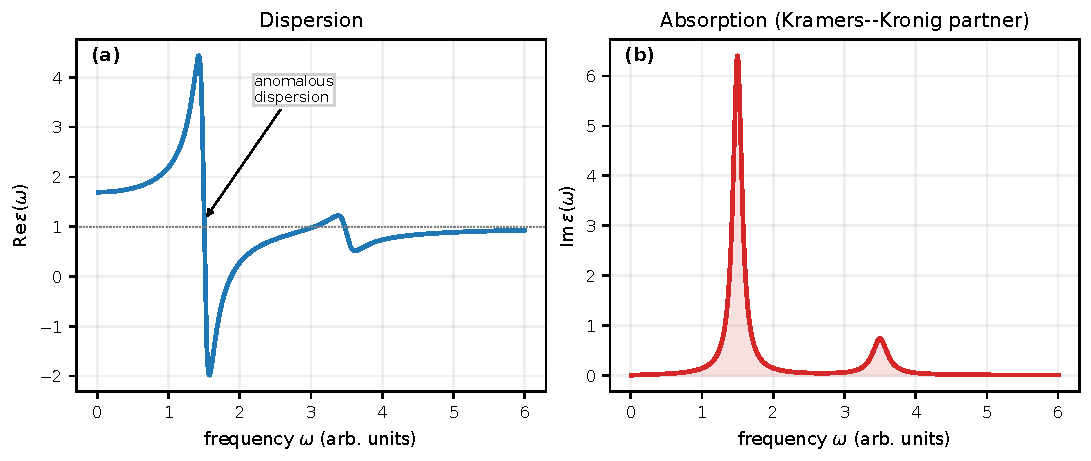
\includegraphics[width=0.95\linewidth]{fig_f5_kramers_kronig.pdf}
 \caption{Complex permittivity of a two-resonance Lorentz model
 ($\omega_{01} = 1.5$, $\omega_{02} = 3.5$; damping
 $\gamma_1 = 0.15$, $\gamma_2 = 0.25$; arbitrary units).
 (a)~Real part $\Re\varepsilon(\omega)$ showing normal and anomalous
 dispersion near each resonance; the dotted line marks the
 high-frequency limit $\varepsilon = 1$.
 (b)~Imaginary part $\Im\varepsilon(\omega)$, the
 Kramers--Kronig partner of~(a). Each absorption peak in~(b)
 corresponds to a region of anomalous dispersion in~(a),
 as required by causality. For a passive medium,
 $\Im\varepsilon > 0$ at all positive frequencies.}
 \label{fig:kramers-kronig-lorentz}
\end{figure}


\subsection{Multiple resonances and the Drude model}
\label{ssec:multi-resonance}

A real material has multiple absorption lines at frequencies
$\omega_{0j}$, each with its own oscillator strength $f_j$ and damping
$\gamma_j$. The total permittivity is
\begin{equation}
 \epsr(\omega) = 1 + \sum_j \frac{f_j\,\omega_p^2}
 {\omega_{0j}^2 - \omega^2 - i\gamma_j\omega},
 \qquad
 \sum_j f_j = 1.
 \label{eq:multi-lorentz}
\end{equation}
The sum rule $\sum_j f_j = 1$ (Thomas--Reiche--Kuhn sum rule)~\cite{al2024topological} is a
consequence of the commutation relation $[x,p] = i\hbar$ and ensures
that the high-frequency behavior is
$\epsr(\omega) \to 1 - \omega_p^2/\omega^2$ regardless of the number of
resonances.

In metals and doped semiconductors, free carriers have no restoring force
($\omega_{0} = 0$), and the corresponding contribution is the
\emph{Drude} model:
\begin{equation}
 \varepsilon_{\mathrm{Drude}}(\omega)
 = 1 - \frac{\omega_p^2}{\omega(\omega + i\gamma_D)},
 \label{eq:drude}
\end{equation}
where $\gamma_D$ is the Drude damping rate (scattering rate). At low
frequencies, $\Im\varepsilon_{\mathrm{Drude}} \propto 1/\omega$:
the absorption diverges, reflecting the dc conductivity
$\sigma_0 = \epsvac\omega_p^2/\gamma_D$. At optical frequencies, the
Drude response produces a negative real permittivity for
$\omega < \omega_p$, which is the origin of the metallic reflectivity
and supports surface plasmon polaritons.

\begin{figure}[t]
 \centering
 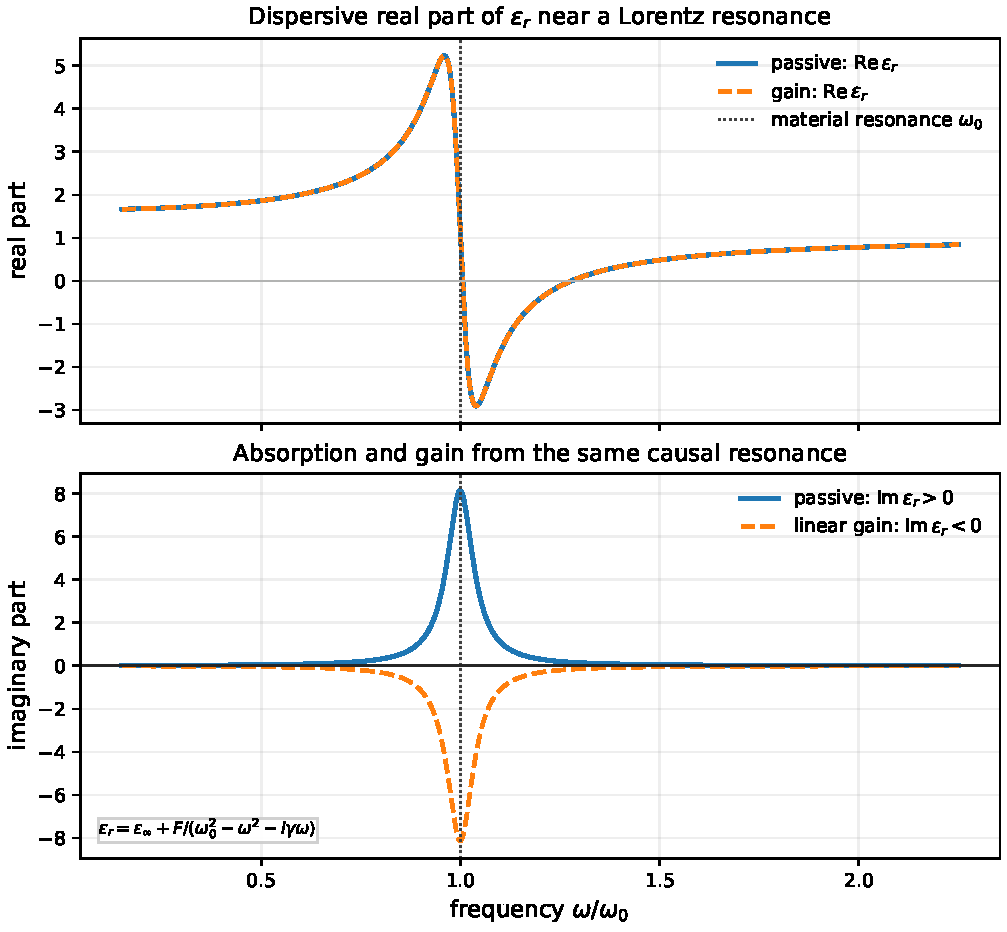
\includegraphics[width=0.92\textwidth]{fig_f5_lorentz_dispersion.pdf}
 \caption{Lorentz dispersion as the simplest Maxwell material model of
 loss and gain. The same resonance produces a dispersive real
 permittivity and a peaked imaginary response. With the $e^{-i\omega t}$
 convention, positive damping gives $\Im\epsr>0$ (absorption), while the
 sign-reversed linear model gives $\Im\epsr<0$ (gain).}
 \label{fig:lorentz-dispersion}
\end{figure}


%% ================================================================
\section{Kramers--Kronig relations}
\label{sec:kramers-kronig}

\subsection{Derivation from causality}
\label{ssec:kk-derivation}

The causality of the susceptibility kernel---$\chi(\tau) = 0$ for
$\tau < 0$---implies that $\hat{\chi}(\omega)$ is analytic in the upper
half of the complex $\omega$ plane (UHP). The derivation proceeds as
follows:

Consider the integral of $\hat{\chi}(\omega')/(\omega'-\omega)$ around a
closed contour $\mathcal{C}$ in the UHP consisting of: (i) the real axis
from $-R$ to $R$ with a small semicircular indent of radius $\epsilon$
above the pole at $\omega' = \omega$, and (ii) a large semicircle of
radius $R$ in the UHP.

Since $\hat{\chi}(\omega')$ is analytic in the UHP (by causality) and
vanishes on the large semicircle as $R \to \infty$ (by the Riemann--Lebesgue
lemma, since $\chi(\tau)$ is integrable), Cauchy's integral theorem gives
\begin{equation}
 \oint_{\mathcal{C}} \frac{\hat{\chi}(\omega')}{\omega'-\omega}\;\dd\omega' = 0.
 \label{eq:cauchy-contour}
\end{equation}
The contributions from the real axis give the principal-value integral,
and the small semicircular indent contributes $-i\pi\hat{\chi}(\omega)$.
Setting the total to zero and separating real and imaginary parts yields
the \emph{Kramers--Kronig relations}~\cite{sols2021functional}:
\begin{align}
 \epsr'(\omega) - 1 &= \frac{1}{\pi}\,\mathcal{P}\!\!
 \int_{-\infty}^{\infty}\frac{\epsr''(\omega')}{\omega' - \omega}
 \;\dd\omega',
 \label{eq:kk-real}\\[4pt]
 \epsr''(\omega) &= -\frac{1}{\pi}\,\mathcal{P}\!\!
 \int_{-\infty}^{\infty}\frac{\epsr'(\omega') - 1}{\omega' - \omega}
 \;\dd\omega'.
 \label{eq:kk-imag}
\end{align}
These relations are not a model: they are exact consequences of causality
and linearity.

\subsection{Physical consequences}
\label{ssec:kk-physics}

\begin{takeaway}[Dispersion and absorption are inseparable]
The Kramers--Kronig relations show that the real and imaginary parts of
$\epsr(\omega)$ are not independent. A medium that absorbs at some
frequencies \emph{must} disperse at all frequencies, and vice versa.
A frequency-independent but lossy $\epsr$ violates causality. This
constraint is important for non-Hermitian photonics: any model with
complex $\epsr$ must be checked for Kramers--Kronig consistency, or it
describes an unphysical material.
\end{takeaway}

\subsection{Sum rules}
\label{ssec:sum-rules}

Specializing the Kramers--Kronig relations to $\omega = 0$ or
$\omega \to \infty$ yields useful sum rules. The $f$-sum rule connects
the total absorption to the electron density:
\begin{equation}
 \int_0^\infty \omega\,\epsr''(\omega)\;\dd\omega
 = \frac{\pi}{2}\,\omega_p^2,
 \label{eq:f-sum-rule}
\end{equation}
where $\omega_p$ is the plasma frequency. This result is exact for any
causal response function and provides a powerful check on material models
and experimental data.

\begin{figure}[t]
 \centering
 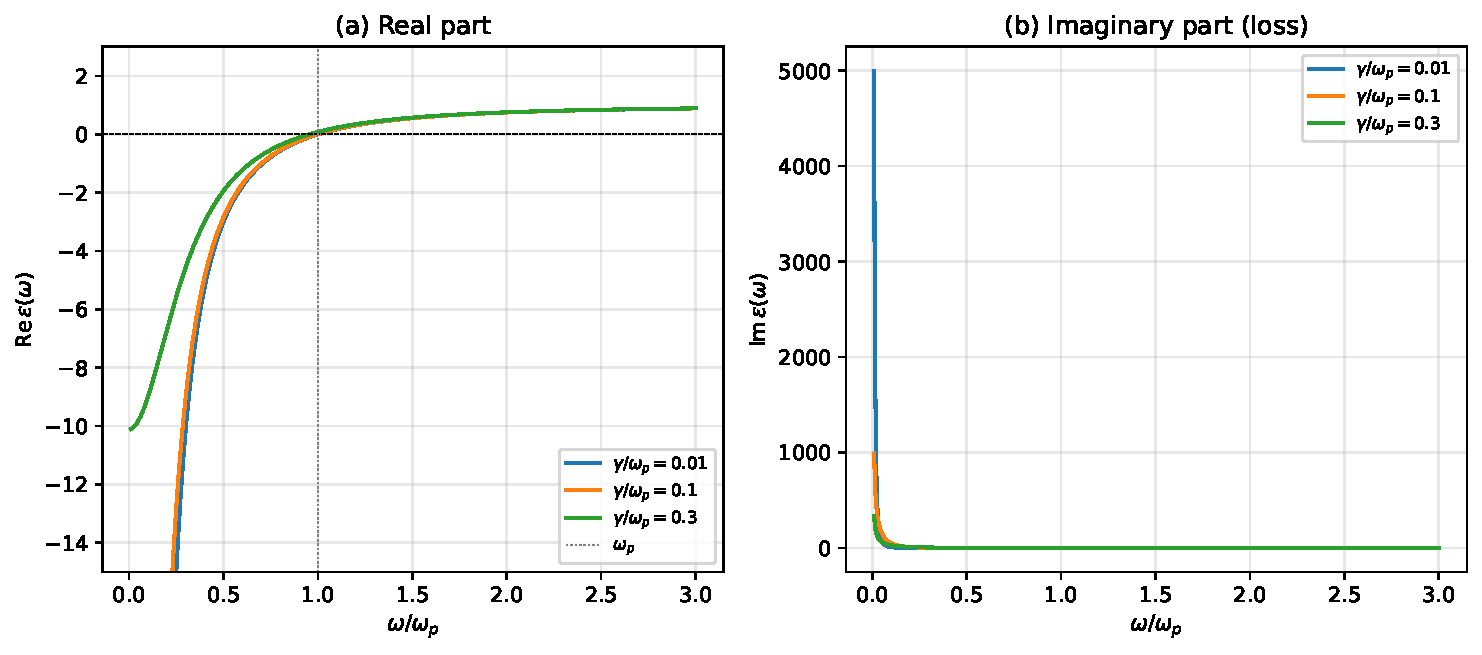
\includegraphics[width=0.85\linewidth]{figures/fig_f05_drude_permittivity.pdf}
 \caption{Drude permittivity for a free-electron metal.
 (a)~$\Re\,\varepsilon(\omega)$ is negative below the plasma frequency
 $\omega_p$ (vertical dotted line) and approaches $+1$ at high
 frequencies. Increasing the damping rate $\gamma$ smooths the
 divergence near $\omega = 0$.
 (b)~$\Im\,\varepsilon(\omega)$ is peaked at low frequencies where
 ohmic absorption dominates. The interplay of negative
 $\Re\,\varepsilon$ and finite $\Im\,\varepsilon$ is the origin of
 plasmonic resonances in metallic nanostructures.}
 \label{fig:drude-permittivity}
\end{figure}

\subsection{Passivity and the power dissipation condition}
\label{ssec:passivity}

A passive medium absorbs more energy than it emits at every frequency.
This imposes the \emph{power dissipation condition}:
\begin{equation}
 \omega\,\epsr''(\omega) \ge 0
 \qquad\text{for all real } \omega.
 \label{eq:passivity}
\end{equation}
For positive frequencies, this means $\epsr'' \ge 0$: absorption. For
an active (gain) medium, $\epsr'' < 0$ at some positive frequencies,
violating passivity. Gain media are driven out of thermodynamic
equilibrium by an external pump (optical or electrical), and the
Kramers--Kronig relations must be applied to the full response including
the pump-induced changes~\cite{figotin2004hamiltonian}.


%% ================================================================
\section{Energy in lossy and dispersive media}
\label{sec:dispersive-energy}

The time-averaged energy density~\eqref{eq:time-avg-u} was derived for
real, nondispersive $\epsr$. When $\epsr(\omega)$ is complex and
frequency-dependent, the energy stored in the medium is no longer given
by $\frac{1}{4}\epsvac\epsr|\EE|^2$.

\subsection{The Brillouin formula}
\label{ssec:brillouin}

For a lossless dispersive medium, or for a low-loss medium observed over a
transparent narrow band centered at frequency $\omega_0$, the
time-averaged energy density is approximately
\begin{equation}
 \langle u\rangle_{\mathrm{disp}}
 = \frac{1}{4}\epsvac\,
 \dv{}{\omega}\!\bigl[\omega\,\epsr'(\omega)\bigr]
 \bigg|_{\omega_0}\!\!|\EE|^2
 + \frac{1}{4}\muvac\,
 \dv{}{\omega}\!\bigl[\omega\,\mur'(\omega)\bigr]
 \bigg|_{\omega_0}\!\!|\HH|^2.
 \label{eq:brillouin-full}
\end{equation}
This is the \emph{Brillouin formula}, widely used in textbooks. It
reduces to the nondispersive result when $\epsr$ is constant.

However, the Brillouin formula has severe limitations:
\begin{enumerate}
 \item It assumes a transparent or weakly absorbing frequency window, so
 that a stored energy can be separated cleanly from irreversible heat.
 \item Near an absorption resonance, using only the real part of a
 lossy permittivity can give misleading or even negative apparent
 ``energy densities.''
 \item It accounts for material polarization energy only indirectly,
 through the frequency derivative of the constitutive parameters.
 \item It cannot be used as an inner product for mode
 orthogonality, because it depends on $\omega$ and is not bilinear.
\end{enumerate}

\subsection{Example: energy density near a Lorentz resonance}
\label{ssec:brillouin-lorentz}

For the single Lorentz oscillator~\eqref{eq:lorentz-eps} in the lossless
limit $\gamma\to 0$, the Brillouin energy factor is
\begin{equation}
 \dv{}{\omega}\bigl[\omega\,\epsr'(\omega)\bigr]
 = 1 + \omega_p^2\,
 \frac{\omega_0^2 + \omega^2}{(\omega_0^2-\omega^2)^2}.
 \label{eq:brillouin-lorentz}
\end{equation}
Away from resonance, this is positive and large, correctly capturing the
additional energy stored in the material polarization. At the resonance
itself the lossless formula
diverges, signaling that the transparent-medium approximation has broken
down. With finite damping, a meaningful energy balance must include the
oscillator and bath degrees of freedom explicitly; substituting only
$\epsr'(\omega)$ into the Brillouin formula is then no longer a reliable
inner product.

\subsection{Why a simple inner product fails}
\label{ssec:no-simple-inner}

The root of the difficulty is that the reduced macroscopic Maxwell
equations---written in terms of $\EE$ and $\HH$ alone---describe an
\emph{open subsystem}: the material degrees of freedom (atomic
oscillators, free carriers, phonons) have been integrated out, leaving
only their effect as a frequency-dependent $\epsr(\omega)$. The full
system (fields plus matter) conserves energy, but the reduced system does
not, because energy flows between the fields and the material oscillators.
Attempting to define a conserved energy for the fields alone is like
trying to define a conserved energy for one particle in a two-body
problem~\cite{figotin2004hamiltonian}.


%% ================================================================
\section{Auxiliary fields and the Hamiltonian embedding}
\label{sec:auxiliary-fields}

The resolution, developed rigorously by Figotin and
Schenker~\cite{figotin2004hamiltonian}, is to \emph{restore} the material
degrees of freedom as explicit auxiliary fields and construct a
conservative extended system.

\subsection{The idea}
\label{ssec:aux-idea}

Consider a medium whose susceptibility $\hat{\chi}(\omega)$ satisfies the
causality, passivity, and Kramers--Kronig conditions. The Lorentz model
\eqref{eq:lorentz-eps} can be written as
\begin{equation}
 \hat{\chi}(\omega)
 = \frac{\omega_p^2}{\omega_0^2 - \omega^2 - i\gamma\omega}
 = \int_0^\infty\!\frac{J(\nu)}{\nu^2 - \omega^2 - i\gamma'\omega}\;\dd\nu,
 \label{eq:spectral-representation}
\end{equation}
where the second form generalizes to any causal susceptibility via a
spectral representation (a continuous distribution of oscillator strengths
$J(\nu)$). Each oscillator mode at frequency $\nu$ is promoted to an
explicit dynamical variable---an auxiliary field $\mathbf{P}_\nu(\rr,t)$
that couples to $\EE$ and obeys its own equation of motion.

\subsection{Example: single Lorentz pole}
\label{ssec:aux-single-pole}

For a single Lorentz resonance, the auxiliary field is the polarization
density $\mathbf{P}(\rr,t)$. The coupled equations of motion are:
\begin{align}
 \epsvac\pdv{\EE}{t} &= \curl\HH - \pdv{\mathbf{P}}{t},
 \label{eq:aux-ampere}\\
 \muvac\pdv{\HH}{t} &= -\curl\EE,
 \label{eq:aux-faraday}\\
 \pdv[2]{\mathbf{P}}{t} + \gamma\pdv{\mathbf{P}}{t} + \omega_0^2\mathbf{P}
 &= \epsvac\omega_p^2\,\EE.
 \label{eq:aux-oscillator}
\end{align}
Equation~\eqref{eq:aux-oscillator} is the Lorentz oscillator equation.
Taking the Fourier transform and solving for $\mathbf{P}(\omega)$ gives
$\mathbf{P}(\omega) = \epsvac\hat{\chi}(\omega)\EE(\omega)$, recovering
the Lorentz permittivity~\eqref{eq:lorentz-eps}.

The damping term $\gamma\partial\mathbf{P}/\partial t$ is the source of
non-Hermiticity: it represents energy transfer from the coherent
polarization to an incoherent bath. Without it ($\gamma = 0$), the
system~\eqref{eq:aux-ampere}--\eqref{eq:aux-oscillator} is
conservative and can be written in Hamiltonian form.

\subsection{The extended Hamiltonian}
\label{ssec:extended-hamiltonian}

For $\gamma = 0$, define the canonical momentum of the polarization
oscillator as $\mathbf{Q} = \partial\mathbf{P}/\partial t$. The total
energy of the extended system is
\begin{equation}
 \mathcal{H} = \frac{1}{2}\int\!\left[
 \epsvac|\EE|^2 + \muvac|\HH|^2
 + \frac{|\mathbf{Q}|^2}{\epsvac\omega_p^2}
 + \frac{\omega_0^2|\mathbf{P}|^2}{\epsvac\omega_p^2}
 \right]\dd^3r,
 \label{eq:aux-energy}
\end{equation}
which is manifestly positive definite and conserved by the coupled
equations. The first-order form is
\begin{equation}
 i\,\pdv{}{t}
 \begin{pmatrix} \EE \\ \HH \\ \mathbf{P} \\ \mathbf{Q} \end{pmatrix}
 = \hat{\mathcal{H}}_{\mathrm{ext}}
 \begin{pmatrix} \EE \\ \HH \\ \mathbf{P} \\ \mathbf{Q} \end{pmatrix},
 \label{eq:extended-system}
\end{equation}
where $\hat{\mathcal{H}}_{\mathrm{ext}}$ is self-adjoint with respect to
the extended energy inner product~\eqref{eq:aux-energy}.

When the auxiliary fields are eliminated (by solving their equations of
motion in terms of $\EE$), one recovers the original reduced Maxwell
equations with the frequency-dependent $\epsr(\omega)$. But in the
reduced system, the total energy is no longer conserved: some of it has
been transferred to the hidden oscillators.

For $\gamma > 0$, the damping term breaks the Hermiticity of
$\hat{\mathcal{H}}_{\mathrm{ext}}$. The extended system is then
non-conservative, and a further embedding into a larger Hilbert space
(a Lindblad or Caldeira--Leggett bath) is needed for a fully Hamiltonian
treatment~\cite{figotin2004hamiltonian}.

\begin{takeaway}[Non-Hermiticity from elimination]
The macroscopic Maxwell equations with frequency-dependent $\epsr(\omega)$
are non-Hermitian not because the physics is non-conservative, but because
the conservative degrees of freedom of the material have been eliminated.
Restoring them through auxiliary fields recovers a Hamiltonian (Hermitian)
description of the full system. This is the third road to non-Hermiticity
identified in Chapter~\ref{ch:energy-inner}: not material loss, not
radiation, but frequency dispersion caused by eliminating material
variables from the Maxwell state.
\end{takeaway}


%% ================================================================
\section{Gain media}
\label{sec:gain-media}

An active (gain) medium has $\epsr''(\omega) < 0$ at frequencies within
the gain bandwidth. Physically, this requires an external energy source
(a pump) that maintains a population inversion or stimulated emission
process.

\subsection{The inverted Lorentz model}
\label{ssec:inverted-lorentz}

The Lorentz oscillator model can be adapted to describe gain by reversing
the sign of the damping: $\gamma \to -|\gamma|$. As a small-signal
phenomenological model near a pumped transition, this gives
\begin{equation}
 \varepsilon_{\mathrm{gain}}(\omega)
 = 1 + \frac{\omega_p^2}
 {\omega_0^2 - \omega^2 + i|\gamma|\omega},
 \label{eq:gain-eps}
\end{equation}
with $\epsr'' < 0$ near $\omega_0$. The medium now amplifies rather than
absorbs. Taken literally over all frequencies, negative damping would be
an unstable linear oscillator; in a real gain medium the pump, finite
bandwidth, and saturation nonlinearity regularize the response.

\subsection{Population inversion and the four-level system}
\label{ssec:population-inversion}

In a real laser medium, gain arises from population inversion between
two electronic levels. The simplest tractable model is the four-level
system with levels $|0\rangle$, $|1\rangle$, $|2\rangle$, $|3\rangle$:
an external pump excites atoms from $|0\rangle$ to $|3\rangle$; rapid
non-radiative decay brings atoms from $|3\rangle$ to $|2\rangle$ (the
upper laser level); stimulated emission occurs on the
$|2\rangle \to |1\rangle$ transition, providing gain at the lasing
frequency $\omega_L = (E_2 - E_1)/\hbar$; and rapid decay from
$|1\rangle$ to $|0\rangle$ empties the lower laser level, maintaining
inversion.

The gain coefficient is proportional to the population difference
$\Delta N = N_2 - N_1 > 0$ and to the transition cross section
$\sigma(\omega)$:
\begin{equation}
 g(\omega) = \sigma(\omega)\,\Delta N,
 \label{eq:gain-coefficient}
\end{equation}
where $\sigma(\omega)$ has a Lorentzian line shape centered at $\omega_L$.
The imaginary permittivity contributed by the gain transition is
$\epsr''(\omega) = -cn\, g(\omega)/\omega < 0$.

\paragraph{Rate equations for the four-level system.}
The steady-state populations are governed by the rate equations.
Because the relaxation rates $\gamma_{32}$ (from $|3\rangle$ to
$|2\rangle$) and $\gamma_{10}$ (from $|1\rangle$ to $|0\rangle$) are
fast, the populations $N_3$ and $N_1$ are approximately zero in steady
state, and the total population satisfies $N_0 + N_2 \approx N_{\mathrm{tot}}$.
The rate equation for the upper laser level is
\begin{equation}
 \dv{N_2}{t} = R_{\mathrm{pump}} - \frac{\sigma(\omega_L)\,I}{\hbar\omega_L}\,\Delta N
 - \frac{N_2}{\tau_{\mathrm{sp}}} = 0,
 \label{eq:rate-equation-n2}
\end{equation}
where $R_{\mathrm{pump}}$ is the pump rate (atoms per unit volume per
unit time), $I$ is the intracavity intensity, $\tau_{\mathrm{sp}}$ is
the spontaneous emission lifetime of the upper level, and the middle
term represents the stimulated emission rate. Since
$N_1 \approx 0$, we have $\Delta N \approx N_2$.

Solving~\eqref{eq:rate-equation-n2} for $N_2$ in steady state:
\begin{equation}
 N_2 = \frac{R_{\mathrm{pump}}\,\tau_{\mathrm{sp}}}
 {1 + I/I_{\mathrm{sat}}},
 \qquad
 I_{\mathrm{sat}} = \frac{\hbar\omega_L}{\sigma(\omega_L)\,\tau_{\mathrm{sp}}},
 \label{eq:saturation-derivation}
\end{equation}
where we identify the small-signal inversion
$\Delta N_0 = R_{\mathrm{pump}}\,\tau_{\mathrm{sp}}$ (the inversion in
the absence of stimulated emission). Substituting into
Eq.~\eqref{eq:gain-coefficient} immediately recovers the saturated gain
formula~\eqref{eq:gain-saturation}:
\begin{equation}
 g(I) = \sigma\,\Delta N_0 \cdot \frac{1}{1 + I/I_{\mathrm{sat}}}
 = \frac{g_0}{1 + I/I_{\mathrm{sat}}}.
 \label{eq:gain-saturation-derived}
\end{equation}
The saturation intensity $I_{\mathrm{sat}}$ has a transparent physical
meaning: it is the intensity at which the stimulated emission rate
$\sigma I/(\hbar\omega_L)$ equals the spontaneous decay rate
$1/\tau_{\mathrm{sp}}$. Below this intensity, stimulated emission is a
small perturbation on the inversion; above it, stimulated emission
dominates and the gain is depleted.

\paragraph{Gain clamping and threshold.}
At steady-state lasing, the gain must exactly compensate the total cavity
loss $\alpha_{\mathrm{tot}}$ (including mirror loss and material
absorption):
\begin{equation}
 g(I_{\mathrm{ss}}) = \alpha_{\mathrm{tot}} \quad\Rightarrow\quad
 I_{\mathrm{ss}} = I_{\mathrm{sat}}\left(\frac{g_0}{\alpha_{\mathrm{tot}}} - 1\right).
 \label{eq:gain-clamping}
\end{equation}
This is the gain-clamping condition. Below threshold
($g_0 < \alpha_{\mathrm{tot}}$), no steady-state lasing occurs and
$I_{\mathrm{ss}} = 0$. Above threshold, the intracavity intensity
grows linearly with pump power (since $g_0 \propto R_{\mathrm{pump}}$),
while the material gain clamps at $\alpha_{\mathrm{tot}}$---it cannot
exceed the loss, because any excess gain would increase $I$, which would
further deplete the inversion until balance is restored.

\paragraph{Connection to the Maxwell framework.}
The gain-clamping condition connects the microscopic rate equations to
the macroscopic Maxwell eigenproblem. The intensity-dependent
permittivity of the gain medium is
\begin{equation}
 \epsr(\omega, I) = \epsr'(\omega)
 - i\,\frac{c\,n_{\mathrm{bg}}\,g(I)}{\omega}
 = \epsr'(\omega)
 - i\,\frac{c\,n_{\mathrm{bg}}\,g_0}{\omega(1 + I/I_{\mathrm{sat}})},
 \label{eq:eps-saturated}
\end{equation}
where $n_{\mathrm{bg}}$ is the background refractive index and the
negative sign of the imaginary part reflects gain (with our
$e^{-i\omega t}$ convention, $\epsr'' < 0$ corresponds to
amplification). This intensity-dependent permittivity makes the
Maxwell eigenproblem nonlinear: the eigenfrequencies depend on the
field amplitudes through $I$. The linear non-Hermitian framework
of this book treats $\epsr$ as independent of $I$---an approximation
valid below or near threshold, where $I \ll I_{\mathrm{sat}}$ and
$g \approx g_0$. Above threshold, the full nonlinear problem must
be solved self-consistently, as discussed in
Chapter~\ref{ch:open-problems}.

\subsection{Gain saturation}
\label{ssec:gain-saturation}

As the intracavity field intensity $I$ grows, stimulated emission depletes
the population inversion. The saturated gain coefficient is
\begin{equation}
 g(I) = \frac{g_0}{1 + I/I_{\mathrm{sat}}},
 \label{eq:gain-saturation}
\end{equation}
where $g_0$ is the small-signal gain and $I_{\mathrm{sat}}$ is the
saturation intensity. At threshold, the saturated gain equals the total
loss. Above threshold, the gain clamps at the loss value, and additional
pump power is converted into laser output power.

\begin{figure}[t]
 \centering
 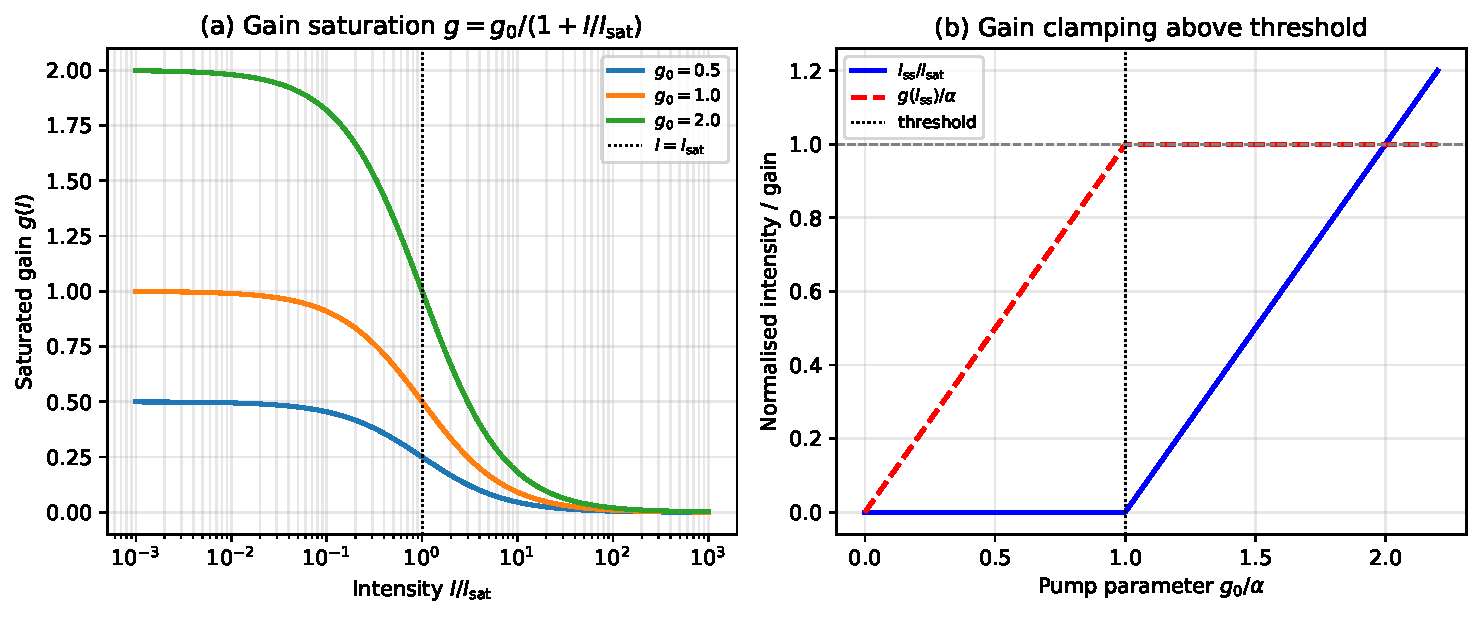
\includegraphics[width=0.85\linewidth]{figures/fig_f05_gain_saturation_rate.pdf}
 \caption{Gain saturation and gain clamping in a four-level laser model.
 (a)~The saturated gain $g(I)=g_0/(1+I/I_{\mathrm{sat}})$ decreases once
 the intracavity intensity becomes comparable with the saturation
 intensity $I_{\mathrm{sat}}$. (b)~Above threshold, the steady-state
 intensity grows as $I_{\mathrm{ss}}/I_{\mathrm{sat}}=g_0/\alpha-1$
 while the material gain clamps to the total loss $\alpha$. This is the
 nonlinear mechanism that prevents the linear gain model from producing
 unbounded fields above threshold.}
 \label{fig:gain-saturation-rate}
\end{figure}


Gain saturation is intrinsically nonlinear: the permittivity depends on
the field amplitude. The linear non-Hermitian framework developed in
this book is therefore strictly valid only below or near the lasing
threshold. Above threshold, the coupling between the gain medium and the
cavity field requires a nonlinear analysis
(Chapter~\ref{ch:open-problems}).

\paragraph{Quantitative example: InGaAsP gain medium.}
For a typical InGaAsP multiple-quantum-well gain medium~\cite{huang2023resonant,koshelev2018nonradiating} at
$\lambda = 1550\;$nm, the small-signal material gain coefficient is
$g_0 \approx 400\;$cm$^{-1}$ at a carrier density
$N = 3 \times 10^{18}\;$cm$^{-3}$, and the saturation intensity is
$I_{\mathrm{sat}} \approx 5 \times 10^{8}\;$W/m$^2$ (corresponding to
a saturation photon density
$n_{\mathrm{ph,sat}} \approx 2.6 \times 10^{15}\;$cm$^{-3}$).
The corresponding imaginary permittivity is
$\varepsilon'' = -cn g_0/\omega \approx -0.031$ at small signal.
For a photonic crystal cavity with mode volume
$V_{\mathrm{mode}} \sim (\lambda/n)^3 \approx 0.05\;\mu$m$^3$ and
$\Qfac = 5000$, the threshold condition
$g_{\mathrm{th}} = \omega/(c\,\Qfac) \approx 40\;$cm$^{-1}$ is reached
at a pump current of roughly $50\;\mu$A---well within the linear regime
where $g/g_0 \approx 0.1$ and saturation corrections are small. As the
pump increases toward $g_0$, the saturation nonlinearity becomes
important and the linear non-Hermitian description begins to break down.

\begin{figure}[t]
 \centering
 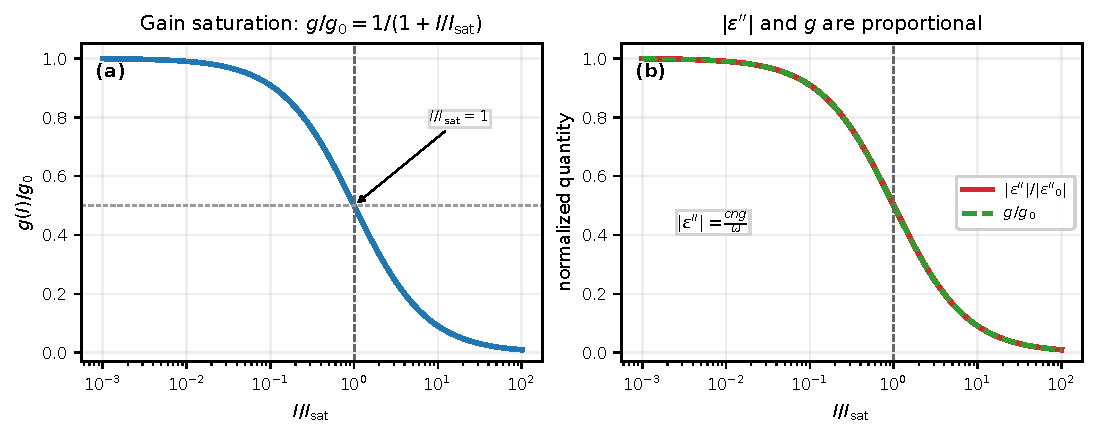
\includegraphics[width=0.96\linewidth]{fig_f5_gain_saturation.pdf}
 \caption{Gain saturation in a homogeneous medium.
 (a)~Normalized gain $g(I)/g_0 = 1/(1+I/I_{\mathrm{sat}})$ versus
 intensity. The half-gain point occurs at $I = I_{\mathrm{sat}}$.
 (b)~Normalized $|\varepsilon''|/|\varepsilon''_0|$ (solid red) and
 $g/g_0$ (dashed green) plotted on the same vertical scale, confirming
 that both quantities share the same saturation dependence; the
 conversion is $|\varepsilon''| = c\,n\,g/\omega$. Parameters:
 $g_0 = 400\;\mathrm{cm}^{-1}$,
 $\varepsilon''_0 \approx -0.031$,
 $\lambda = 1550\;\mathrm{nm}$,
 $n_{\mathrm{eff}} = 3.4$.}
 \label{fig:gain-saturation}
\end{figure}

\paragraph{Kramers--Kronig constraints on gain media.}
A gain medium with $\varepsilon''(\omega) < 0$ over a spectral band~\cite{rter2010observation,feng2012experimental}
must, by the Kramers--Kronig relations, also exhibit anomalous
dispersion $\dd\varepsilon'/\dd\omega < 0$ within the same band. This
is because the subtracted dispersion relation
$\varepsilon'(\omega) - \varepsilon'(\infty) =
(2/\pi)\,\mathcal{P}\!\int_0^\infty
\omega'\varepsilon''(\omega')/(\omega'^2-\omega^2)\;\dd\omega'$
has the same structure for gain as for loss, with reversed sign of
$\varepsilon''$. The anomalous dispersion in the gain band reduces the
group velocity and can even make it superluminal or negative, though the
signal velocity remains bounded by $c$ because the gain bandwidth is
always finite. This connection between gain and anomalous dispersion is
important for understanding the frequency-pulling effect in lasers and
the bandwidth limitations of optical amplifiers.


%% ================================================================
\section{Balanced gain and loss: the $\PT$-symmetric condition}
\label{sec:pt-preview}

A medium with spatial regions of loss and gain, arranged so that
\begin{equation}
 \epsr(\rr) = \epsr^*(-\rr),
 \label{eq:pt-condition-preview}
\end{equation}
has a special symmetry: $\PT$ symmetry. The real part of $\epsr$ is
symmetric and the imaginary part is antisymmetric under spatial inversion.
This condition ensures that the total gain and loss are balanced, and the
system can exhibit a phase transition from real to complex eigenfrequencies.
The physics of $\PT$-symmetric optical systems is the subject of
Chapter~\ref{ch:pt-symmetric}.

\subsection{The $\PT$-symmetric Lorentz model}
\label{ssec:pt-lorentz}

A one-dimensional $\PT$-symmetric refractive-index profile can be
constructed from two Lorentz media with opposite signs of damping:
\begin{equation}
 \epsr(x,\omega) = \begin{cases}
 \eps_{\mathrm{bg}} + \Delta\eps_{\mathrm{Lorentz}}(\omega;\gamma) & x > 0,\\
 \eps_{\mathrm{bg}} + \Delta\eps_{\mathrm{Lorentz}}(\omega;-\gamma) & x < 0,
 \end{cases}
 \label{eq:pt-lorentz-profile}
\end{equation}
where $\gamma > 0$ and $\eps_{\mathrm{bg}}$ is real. This satisfies
$\epsr(x,\omega)=\epsr^*(-x,\omega)$ on the real-frequency axis and provides a
microscopically motivated realization of the $\PT$ condition for the
transfer-matrix and coupled-mode analyses of
Chapter~\ref{ch:pt-symmetric}.


%% ================================================================
\section{Summary and connections}
\label{sec:ch5-forward}

Material loss, gain, and dispersion---the first road to
non-Hermiticity---are not ad hoc modifications of Maxwell's
equations but an inevitable consequence of the causal, dissipative
response of real materials:

\begin{itemize}
 \item Linear response and causality require $\epsr(\omega)$ to be
 complex and frequency-dependent, constrained by the
 Kramers--Kronig relations and sum rules.
 \item The imaginary part $\epsr''$ breaks the self-adjointness of the
 Maxwell operator by making the constitutive weight complex and by
 allowing irreversible exchange of energy with the material.
 \item The Brillouin formula provides a useful but limited
 approximation to the energy in dispersive media; a rigorous
 treatment requires auxiliary fields and an extended Hamiltonian.
 \item Gain media violate passivity through population inversion and
 can lead to lasing when coupled with feedback; gain saturation
 makes the linear non-Hermitian description valid only near or
 below threshold.
 \item The special case of balanced gain and loss ($\PT$ symmetry)
 connects to a rich phenomenology explored in
 Chapter~\ref{ch:pt-symmetric}.
\end{itemize}

Several threads connect forward from this material foundation:
\begin{enumerate}
 \item The complex QNM frequencies of Chapter~\ref{ch:qnm} arise from
 material loss ($\varepsilon'' > 0$) combined with radiative loss
 from open boundaries.
 \item The $\PT$-symmetric condition
 $\varepsilon(\rr) = \varepsilon^*(-\rr)$ of
 Chapter~\ref{ch:pt-symmetric} is a precise spatial arrangement of
 the gain and loss physics developed here.
 \item The dispersive auxiliary-field formulation of
 Section~\ref{sec:auxiliary-fields} reappears in
 Chapter~\ref{ch:numerics} as the basis for finite-element
 eigensolvers that handle frequency-dependent materials without
 nonlinear eigenvalue problems.
 \item Gain saturation provides the nonlinear feedback that stabilises
 lasers and creates the nonlinear exceptional points discussed in
 Chapters~\ref{ch:pt-symmetric} and~\ref{ch:open-problems}.
 \item The Kramers--Kronig constraint that gain media must exhibit
 anomalous dispersion limits the bandwidth of optical amplifiers and
 modifies the group velocity of pulses propagating through active
 photonic structures.
\end{enumerate}

Chapter~\ref{ch:qnm} now turns to the second physical origin of
non-Hermiticity---radiation and openness---and develops the quasinormal-mode
theory that provides the natural eigenstates of the non-self-adjoint
Maxwell operator.

\begin{takeaway}[Material non-Hermiticity is physical, not mathematical]
Complex permittivity, frequency dispersion, gain saturation, and
auxiliary-field embeddings are not formal devices introduced for
mathematical convenience. They encode the irreversible exchange of
energy between the electromagnetic field and matter---absorption heating,
stimulated emission, and the frequency-dependent phase response of bound
electrons. Every non-Hermitian photonic phenomenon studied in the
remainder of this book has its material origin in the physics of this
chapter.
\end{takeaway}

\chapter{Quasinormal Modes}
\label{ch:qnm}

\begin{chapterlead}
When a photonic resonator is open to its environment, its ``modes'' are
not the orthogonal, real-frequency eigenstates of Hermitian spectral
theory. They are \emph{quasinormal modes}: solutions of the source-free
Maxwell equations with outgoing boundary conditions, possessing complex
eigenfrequencies and field profiles that diverge at spatial infinity.
Quasinormal modes are derived from the Maxwell operator. Their
normalization and inner product differ from those of closed cavities,
and they describe open photonic systems ranging from nanophotonic
cavities to diffraction gratings.
\end{chapterlead}


%% ================================================================
\section{Defining quasinormal modes}
\label{sec:qnm-definition}

A \emph{quasinormal mode} (QNM) of an open electromagnetic system is a
solution to the source-free vector Helmholtz equation
\begin{equation}
 \curl\!\left[\frac{1}{\epsr(\rr)}\,\curl\tilde{\HH}_n(\rr)\right]
 = \frac{\omtil_n^2}{c^2}\,\tilde{\HH}_n(\rr),
 \label{eq:qnm-evp}
\end{equation}
subject to the \emph{outgoing-wave} (Silver--M\"uller) boundary condition
introduced in Section~\ref{sec:outgoing-bc}. The tilde distinguishes QNM
fields and frequencies from their Hermitian counterparts.

Because the boundary condition is frequency-dependent, the problem is
nonlinear in $\omtil$: we seek pairs $(\omtil_n, \tilde{\HH}_n)$
simultaneously. For a passive system without gain, all QNM frequencies
lie in the lower half of the complex $\omega$ plane:
\begin{equation}
 \omtil_n = \omega_n - i\gamma_n, \qquad \gamma_n > 0,
 \label{eq:qnm-freq}
\end{equation}
where $\omega_n$ is the resonant frequency and $\gamma_n$ the radiative
decay rate. The quality factor is $\Qfac_n = \omega_n/(2\gamma_n)$.

As established in Section~\ref{sec:poles-zeros-ch4}, the QNM frequencies
coincide with the poles of the scattering matrix $\Smat(\omega)$: at
$\omega = \omtil_n$, an outgoing field exists with no incoming excitation.

\subsection{Example: Fabry--P\'erot QNMs}
\label{ssec:qnm-fabry-perot}

The simplest system with QNMs is a dielectric slab of thickness $L$ and
real refractive index $n$ in vacuum. The QNM condition requires outgoing
waves on both sides, which is equivalent to the round-trip resonance
condition with the Fresnel reflection coefficient
$r = (n-1)/(n+1)$:
\begin{equation}
 r^2 e^{2in\omtil L/c} = 1.
 \label{eq:fp-qnm-condition}
\end{equation}
Solving for $\omtil$ gives the QNM frequencies
\begin{equation}
 \omtil_m = \frac{c}{nL}\left(m\pi - \arg r\right)
 - i\,\frac{c}{nL}\ln\frac{1}{|r|},
 \qquad m = 0, \pm 1, \pm 2, \ldots
 \label{eq:fp-qnm-freqs}
\end{equation}
All frequencies have the same imaginary part
$\gamma = (c/nL)\ln(1/|r|)$, set by the mirror reflectivity. For a
silicon slab ($n = 3.5$, $L = 300\;\mathrm{nm}$):
\begin{itemize}
 \item $|r| = (3.5-1)/(3.5+1) = 0.556$, so $\ln(1/|r|) = 0.588$.
 \item $\gamma = c \times 0.588 / (3.5 \times 300\;\mathrm{nm})
 \approx 1.68 \times 10^{14}\;\mathrm{rad/s}$.
 \item $\Qfac \approx \omega_0/(2\gamma)$. For the fundamental mode
 at $\lambda \approx 2nL = 2100\;\mathrm{nm}$
 ($\omega_0 \approx 8.97 \times 10^{14}\;\mathrm{rad/s}$),
 $\Qfac \approx 2.7$.
\end{itemize}
This very low $\Qfac$ reflects the poor confinement of a bare slab.
Adding distributed Bragg reflectors raises $|r|$ and pushes the QNM
poles closer to the real axis.

\paragraph{QNM field profile inside and outside the slab.}
Inside the slab ($0 < z < L$), the QNM field is a standing wave:
$\tilde{E}_m(z) \propto \sin(n\omtil_m z/c)$ (for the $\EE$-field of a
TE mode at normal incidence). Outside the slab ($z > L$ or $z < 0$),
the field has the outgoing-wave form
$\tilde{E}_m(z) \propto e^{+i\omtil_m z/c}$ for $z > L$ and
$e^{-i\omtil_m z/c}$ for $z < 0$. Writing
$\omtil_m = \omega_m - i\gamma$, the far-field amplitude is
$|\tilde{E}_m(z)| \propto e^{\gamma|z|/c}$: the field grows
exponentially away from the slab, as derived in
Section~\ref{sec:qnm-divergence}. At a distance of
$z = c/\gamma \approx 1.78\;\mu$m (for the silicon slab above), the
field amplitude has grown by a factor of $e \approx 2.72$.
At $z = 10\;\mu$m, it has grown by a factor of $e^{5.6} \approx 270$.
This rapid spatial growth is what makes the standard $L^2$ norm diverge
and necessitates the unconjugated normalization of
Section~\ref{sec:qnm-normalization}.

\begin{figure}[t]
 \centering
 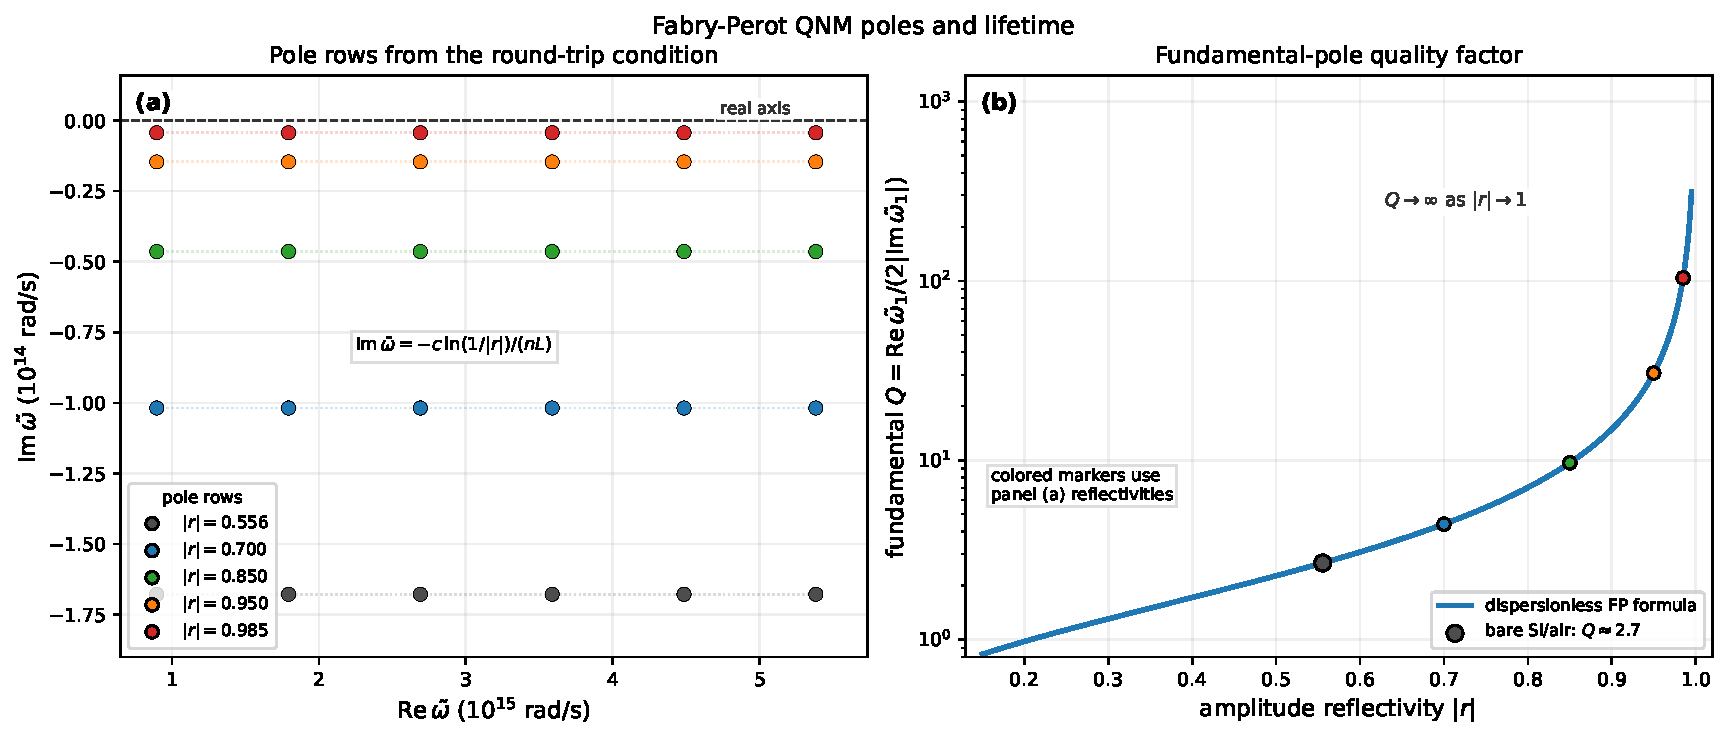
\includegraphics[width=0.92\textwidth]{fig_f6_fabry_perot_qnm.pdf}
 \caption{Quasinormal-mode poles of a one-dimensional Fabry--P\'erot resonator. Panel (a) plots the pole positions from the round-trip condition $r^2\exp(2in\tilde{\omega}L/c)=1$ for several mirror reflectivities; the compact legend identifies the $|r|$ value for each pole row, and the in-panel formula gives the imaginary part $\mathrm{Im}\,\tilde{\omega}=-c\ln(1/|r|)/(nL)$. Increasing $|r|$ moves the pole rows upward toward the real-frequency axis while remaining in the passive lower half-plane. Panel (b) shows the fundamental quality factor $Q=\mathrm{Re}\,\tilde{\omega}_1/(2|\mathrm{Im}\,\tilde{\omega}_1|)$ as a function of amplitude reflectivity, with colored markers corresponding to the same $|r|$ values as the pole rows. The gray marker denotes the bare silicon--air interface example used in the text, with $n=3.5$, $L=300\,\mathrm{nm}$, $|r|=0.556$, and $Q\approx2.67$.}
 \label{fig:fabry-perot-qnm-poles}
\end{figure}


%% ================================================================
\section{Spatial divergence and its physical meaning}
\label{sec:qnm-divergence}

A QNM with complex frequency $\omtil_n = \omega_n - i\gamma_n$ has far-field
spatial behavior
\begin{equation}
 \tilde{\HH}_n(\rr) \;\sim\;
 \frac{e^{i\omtil_n r/c}}{r}\,\mathbf{f}_n(\hat{\rr})
 = \frac{e^{i\omega_n r/c}\,e^{\gamma_n r/c}}{r}\,\mathbf{f}_n(\hat{\rr}),
 \label{eq:qnm-farfield}
\end{equation}
where $\mathbf{f}_n$ is an angular pattern. The factor $e^{\gamma_n r/c}$
\emph{grows} exponentially with distance. This is deeply
counterintuitive---how can a decaying mode grow in space?

The resolution is causal: the QNM represents a field pattern that was
established at some time in the past and has been radiating ever since.
At a distant point $r$, we observe light that was emitted at the earlier
time $t - r/c$, when the mode had amplitude $e^{-\gamma_n(t - r/c)}$.
The product of the temporal decay and the retardation gives
$e^{-\gamma_n t}\,e^{\gamma_n r/c}$: at fixed $t$, the field grows with
$r$ because distant points sample the mode at earlier, stronger times.

This exponential growth means that the standard $L^2$ norm
$\int|\tilde{\HH}_n|^2\;\dd^3 r$ diverges. The QNM is \emph{not
square-integrable} and cannot be normalized with the Hermitian inner
product of Chapter~\ref{ch:energy-inner}. A different normalization
scheme is needed.

\begin{figure}[t]
 \centering
 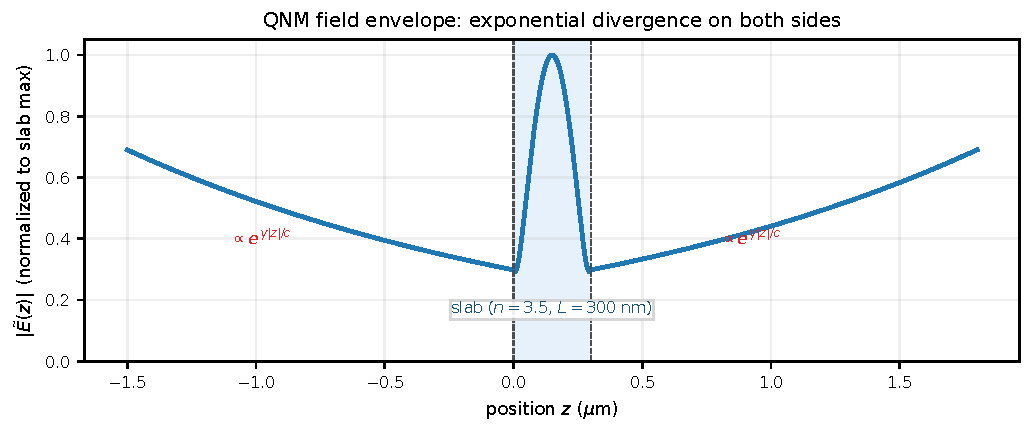
\includegraphics[width=0.92\linewidth]{fig_f6_qnm_divergence.pdf}
 \caption{Field envelope $|\tilde{E}(z)|$ of the fundamental
 quasinormal mode of a dielectric slab ($n = 3.5$,
 $L = 300\;\mathrm{nm}$) in vacuum, normalized to the slab-interior
 maximum. The mode is the symmetric
 $\cos\tilde{k}(z - L/2)$ solution. Outside the slab, the
 outgoing-wave boundary condition produces exponential growth
 $\propto e^{\gamma|z|/c}$ on both sides, where
 $\gamma = -c\ln|r|/(nL)$ is the radiative decay rate from
 Eq.~\eqref{eq:qnm-freq}. This divergence is the defining feature
 of QNMs and is regularized by perfectly matched layers
 (Section~\ref{sec:qnm-pml}). Shaded region marks the slab.}
 \label{fig:qnm-field-divergence}
\end{figure}

\subsection{Connection to the skin effect}
\label{ssec:divergence-skin}

The spatial divergence of a single QNM has a close analogy with the
non-Hermitian skin effect (Chapter~\ref{ch:skin-effect}): in both cases,
the non-Hermitian boundary condition forces eigenstates to have
exponentially growing or decaying spatial profiles rather than the
oscillatory behavior of Hermitian modes. The QNM divergence is the
single-resonator version of a phenomenon that, in periodic systems,
becomes the collective skin effect.

%% ================================================================
\section{PML regularization and the non-self-adjoint operator}
\label{sec:qnm-pml}

The perfectly matched layers introduced in Section~\ref{sec:pml} provide
both a computational tool and a conceptual resolution of the divergence
problem. By applying a complex coordinate stretching $\rr \to \tilde{\rr}$
in the absorbing layer, the PML maps the outgoing-wave problem on an
infinite domain to an eigenvalue problem on a bounded domain with a
\emph{non-self-adjoint} operator~\cite{vial2014quasimodal}.

\subsection{How PML regularization works}
\label{ssec:pml-mechanism}

In the PML-regularized problem:
\begin{enumerate}
 \item The QNM fields are damped in the PML region and become
 square-integrable on the computational domain.
 \item The true QNM eigenfrequencies $\omtil_n$ (poles of $\Smat$) are
 unchanged---they are intrinsic to the scatterer and independent
 of the PML parameters.
 \item The continuous spectrum of radiation modes is discretized by the
 finite PML, producing a set of ``PML modes'' that depend on the
 PML thickness and absorption strength.
 \item The transformed Maxwell operator is non-self-adjoint: its
 eigenvectors are not orthogonal under the standard $L^2$ inner
 product.
\end{enumerate}

\subsection{PML validation and spurious modes}
\label{ssec:pml-validation}

The PML introduces two practical concerns:
\begin{itemize}
 \item \textbf{Spurious PML modes:} the discretized radiation continuum
 produces a set of modes whose eigenfrequencies depend on the PML
 parameters. These must be distinguished from the physical QNMs,
 whose eigenfrequencies converge as the PML thickness and absorption
 increase. A standard check is to vary the PML parameters and
 identify eigenfrequencies that remain stable.
 \item \textbf{PML thickness and absorption:} the PML must be thick
 enough and absorbing enough to suppress reflections from the outer
 boundary. For QNMs with large $\gamma_n$ (low $\Qfac$), the spatial
 growth rate $\gamma_n/c$ is large, and the PML must compensate this
 growth before the field reaches the outer boundary. A rule of thumb
 is that the PML absorption over its thickness should provide at least
 $20\;\mathrm{dB}$ of suppression.
\end{itemize}

The price of PML regularization is that the operator is now manifestly
non-Hermitian. The tools of Hermitian spectral theory do not apply.
Instead, we must use the \emph{adjoint} operator and \emph{biorthogonal}
relations.

\paragraph{PML convergence in practice~\cite{opg2023dispersive,v2024exact}.}
For the silicon Fabry--P\'erot slab ($n = 3.5$, $L = 300\;\mathrm{nm}$),
a PML of thickness $d_{\mathrm{PML}} = 2\lambda$ with a quadratic
absorption profile $\sigma(s) = \sigma_{\max}(s/d_{\mathrm{PML}})^2$
converges the fundamental QNM frequency to four significant figures once
$\sigma_{\max} \gtrsim 3\,\omega/c$. Beyond that value the pole
position is insensitive to PML parameters---the hallmark of a
well-converged QNM calculation, because the physical eigenfrequency is a
property of the resonator, not of the absorbing boundary. A useful
convergence diagnostic is the mode ratio
$\eta = |\tilde{E}_{\mathrm{PML,outer}}|/|\tilde{E}_{\max}|$: when
$\eta < 10^{-3}$, the field has decayed sufficiently within the PML and
the eigenvalue is converged to better than $0.1\%$. This criterion
translates into a minimum PML thickness of roughly $1.5$--$2$ wavelengths
for moderate-$\Qfac$ resonators ($\Qfac \sim 10$) and can be relaxed to
$\sim 1\lambda$ for high-$\Qfac$ modes ($\Qfac > 10^3$) whose
far-field divergence rate $\gamma/c$ is small.


%% ================================================================
\section{The adjoint problem and biorthogonality}
\label{sec:qnm-adjoint}

\subsection{The adjoint Maxwell operator}
\label{ssec:adjoint-operator}

For the PML-regularized Maxwell operator $\Mop_{\mathrm{PML}}$, the
adjoint operator $\Mop_{\mathrm{PML}}^\adj$ is defined by the condition
\begin{equation}
 \langle\mathbf{F},\,\Mop_{\mathrm{PML}}\mathbf{G}\rangle
 = \langle\Mop_{\mathrm{PML}}^\adj\mathbf{F},\,\mathbf{G}\rangle
 \label{eq:adjoint-def}
\end{equation}
for all fields in the domain. For a reciprocal medium (symmetric
$\epsr$ tensor), the adjoint operator takes a remarkably simple form:
its eigenvectors $\tilde{\HH}_n^{\mathrm{L}}$ satisfy the same
differential equation~\eqref{eq:qnm-evp} but with \emph{incoming-wave}
boundary conditions---the time-reverse of the QNM
problem~\cite{vial2014quasimodal}.

\subsection{Biorthogonality}
\label{ssec:biorthogonality}

The ``left'' (adjoint) eigenvectors $\tilde{\HH}_m^{\mathrm{L}}$ and
``right'' (direct) eigenvectors $\tilde{\HH}_n$ satisfy a biorthogonality
relation:
\begin{equation}
 \bigl\langle\tilde{\HH}_m^{\mathrm{L}},\,
 \tilde{\HH}_n\bigr\rangle_{\mathrm{PML}}
 = \delta_{mn},
 \label{eq:biorthogonality}
\end{equation}
after appropriate normalization. This is the non-Hermitian analogue of
mode orthogonality. The subscript PML indicates that the integral is over
the computational domain including the PML region.

\subsection{Physical interpretation}
\label{ssec:biorthogonal-physics}

The biorthogonality relation has a direct physical interpretation:
$\langle\tilde{\HH}_m^{\mathrm{L}}|\tilde{\HH}_n\rangle = 0$ for
$m \neq n$ means that the \emph{time-reversed} field of mode $m$
has zero overlap with the forward field of mode $n$. This is a
statement about reciprocity: the mode $m$ launched backward does not
excite mode $n$ launched forward. This reciprocal orthogonality replaces
the power orthogonality of Hermitian modes.

\begin{booknote}[Biorthogonality replaces orthogonality]
In Hermitian systems, left and right eigenvectors are simply complex
conjugates of each other, and the biorthogonality
relation~\eqref{eq:biorthogonality} reduces to ordinary orthogonality
$\langle\HH_m^*,\HH_n\rangle = \delta_{mn}$. In non-Hermitian systems,
left and right eigenvectors are generally different functions, and the
bilinear form $\langle\cdot,\cdot\rangle$ is not the same as the
Hermitian inner product $\langle\cdot|\cdot\rangle$.
\end{booknote}


%% ================================================================
\section{QNM normalization}
\label{sec:qnm-normalization}

The normalization of quasinormal modes is subtle because the standard
volume integral diverges. Several equivalent prescriptions exist.

\subsection{The unconjugated norm}
\label{ssec:unconjugated}

For a reciprocal system, the adjoint modes are related to the direct
modes by $\tilde{\HH}_n^{\mathrm{L}}(\rr) = \tilde{\HH}_n(\rr)$
(without complex conjugation), and the normalization condition
becomes~\cite{kristensen2011effective}
\begin{equation}
 \int_\Omega \epsr(\rr)\,\tilde{\EE}_n(\rr)\cdot\tilde{\EE}_n(\rr)
 \;\dd^3 r
 + \text{surface correction}
 = 1.
 \label{eq:unconjugated-norm}
\end{equation}
The crucial feature is that $\tilde{\EE}_n$ appears \emph{twice without
conjugation}: this is an unconjugated bilinear form, not a Hermitian
inner product. The ``norm'' is complex, and the ``mode volume'' derived
from it is also complex:
\begin{equation}
 \tilde{V}_n = \frac{1}{\epsr(\rr_0)\,\tilde{\EE}_n(\rr_0)\cdot
 \tilde{\EE}_n(\rr_0)},
 \label{eq:complex-mode-volume}
\end{equation}
evaluated at a point of interest $\rr_0$ (typically the field maximum).

\subsection{The surface-integral correction}
\label{ssec:surface-correction}

The unconjugated volume integral in~\eqref{eq:unconjugated-norm} still
diverges over infinite space. The PML regularization truncates the domain,
but in formulations without a PML one can add an analytic surface term
that cancels the far-field divergence~\cite{kristensen2011effective}.
For a nondispersive homogeneous exterior the correction has the schematic
form
\begin{equation}
 N_n =
 \int_{\Omega_R}
 \left[
 \epsr\,\tilde{\EE}_n\cdot\tilde{\EE}_n
 - \mur\,\tilde{\HH}_n\cdot\tilde{\HH}_n
 \right]\dd^3 r
 + S_R[\tilde{\EE}_n,\tilde{\HH}_n],
 \label{eq:surface-norm}
\end{equation}
where $\Omega_R$ is a finite volume bounded by a surface of radius $R$
and $S_R$ is an outgoing-wave surface functional determined by the
far-field expansion. Its role is not to add stored energy at the boundary,
but to analytically continue the divergent volume integral to a finite,
normalization-independent value. In modern computations this same
regularization is often achieved more cleanly by integrating the
unconjugated product over a PML-stretched domain.

\subsection{Comparison of normalization schemes}
\label{ssec:norm-comparison}

Three normalization schemes are commonly used in the literature:
\begin{enumerate}
 \item \textbf{PML-based:} integrate the unconjugated product over
 the PML domain. Simplest computationally but depends weakly on
 PML parameters.
 \item \textbf{Surface-corrected:} add the surface integral
 correction~\eqref{eq:surface-norm}. PML-independent to
 exponential accuracy.
 \item \textbf{Pole residue:} extract the normalization from the
 residue of the Green function at the QNM pole. Mathematically
 elegant and manifestly PML-independent, but requires a scattering
 calculation at complex frequency.
\end{enumerate}
All three give the same result when properly implemented. The choice is
a matter of computational convenience.

\subsection{The Petermann factor from the unconjugated norm}
\label{ssec:petermann-from-norm}

The complex mode volume~\eqref{eq:complex-mode-volume} has an imaginary
part that vanishes only when the mode is Hermitian. The ratio of the
Hermitian (conjugated) norm to the unconjugated norm defines the
\emph{Petermann factor}:
\begin{equation}
 K_n = \frac{\displaystyle\int |\tilde{\EE}_n(\rr)|^2\;\dd^3 r}
 {\displaystyle\left|\int
 \tilde{\EE}_n(\rr)\cdot\tilde{\EE}_n(\rr)\;\dd^3 r
 \right|},
 \label{eq:petermann-definition}
\end{equation}
where the numerator uses the conventional conjugated inner product and
the denominator is the absolute value of the unconjugated norm. By the
Cauchy--Schwarz inequality, $K_n \ge 1$, with equality if and only if
$\tilde{\EE}_n$ can be chosen everywhere real---i.e.\ the mode is
Hermitian.

To see why $K_n$ measures excess noise and non-orthogonality, note that
the biorthogonal overlap of mode $n$ with its adjoint partner is
\begin{equation}
 \langle \tilde{\EE}_n^{\mathrm{L}} | \tilde{\EE}_n \rangle
 = \frac{1}{\sqrt{K_n}},
 \label{eq:petermann-phase-rigidity}
\end{equation}
so the \emph{phase rigidity} $r_n = K_n^{-1/2}$ measures how close
the right eigenvector is to the left eigenvector. At an exceptional
point, $\tilde{\EE}_n^{\mathrm{L}} \to \tilde{\EE}_m^{\mathrm{L}}$
(the two adjoint vectors coalesce), the overlap
$\langle \tilde{\EE}_n^{\mathrm{L}} | \tilde{\EE}_n \rangle \to 0$,
and $K_n \to \infty$.

The physical consequences of $K_n > 1$ are threefold. First, modal
non-orthogonality changes the residue of the Green tensor and therefore
the way spontaneous-emission noise and modal response are partitioned
among nearby resonances. In laser theory this is often summarized as a
Petermann enhancement of the effective modal noise. For an isolated mode
one often writes the scaling schematically as
\begin{equation}
 F_P \sim K_n\,\frac{3}{4\pi^2}\left(\frac{\lambda}{n}\right)^3
 \frac{Q}{V_{\mathrm{eff}}},
 \label{eq:purcell-petermann}
\end{equation}
where the precise prefactor depends on the QNM normalization, emitter
position, and the separation from neighboring modes. Second, the
fundamental linewidth of a laser operating on mode $n$ is
broadened by $K_n$ (the Schawlow--Townes linewidth multiplied by $K_n$),
because spontaneous emission into the non-orthogonal mode receives
contributions from all modes with nonzero overlap. Third, the
sensitivity of the eigenfrequency to perturbations scales as
$K_n^{1/2}$, connecting the Petermann factor to the enhanced sensing at
exceptional points discussed in Chapter~\ref{ch:exceptional-points}.

\paragraph{Example: plasmonic nanoparticle.}
For a silver nanoparticle of radius $a = 30\;$nm in air at the
localized surface plasmon resonance ($\lambda \approx 360\;$nm), the
mode volume is $|\tilde{V}| \approx 4 \times 10^{-5}\,\lambda^3$ and
the Petermann factor is $K \approx 1.3$---close to unity because the
mode is nearly Hermitian (low radiation loss). For a plasmonic dimer
with a $2\;$nm gap, the mode hybridization and near-field enhancement
push $K$ to $\sim 3$--$5$, and for coupled cavities tuned near an
exceptional point, $K$ can exceed $10^3$, dominating the noise budget.


%% ================================================================
\section{Modal expansion of the Green tensor}
\label{sec:green-tensor}

The electromagnetic Green tensor $\mathbf{G}(\rr,\rr';\omega)$ describes
the field at $\rr$ due to a point dipole source at $\rr'$. In the
spectral neighborhood of a QNM resonance $\omtil_n$, the Green tensor is
dominated by the QNM contribution:
\begin{equation}
 \mathbf{G}(\rr,\rr';\omega)
 \approx \sum_n
 \frac{c^2\,\tilde{\EE}_n(\rr)\otimes\tilde{\EE}_n(\rr')}
 {2\omtil_n(\omega - \omtil_n)},
 \label{eq:green-qnm}
\end{equation}
where the sum runs over QNMs near $\omega$ and the unconjugated
normalization~\eqref{eq:unconjugated-norm} has been used.

\subsection{Local density of states}
\label{ssec:ldos}

The local density of optical states (LDOS) at position $\rr$ is
proportional to the imaginary part of the Green tensor:
\begin{equation}
 \rho(\rr,\omega)
 = \frac{2\omega}{\pi c^2}\,\Im\!\bigl[\tr\mathbf{G}(\rr,\rr;\omega)\bigr].
 \label{eq:ldos}
\end{equation}
Near a QNM resonance, the LDOS exhibits an approximately Lorentzian peak
with width $2\gamma_n$ (where $\gamma_n = -\Im\omtil_n$ is the
half-width at half-maximum) and amplitude proportional to
$\Qfac_n/\Re\tilde{V}_n$.

\subsection{Purcell factor}
\label{ssec:purcell}

The Purcell factor---the enhancement of the spontaneous emission rate of
a quantum emitter at $\rr_0$ relative to free space~\cite{ren2021quasinormal,sauvan2014modal}---is the dipole-projected LDOS ratio
\begin{equation}
 F_P =
 \frac{\hat{\mathbf{d}}\cdot\Im\mathbf{G}(\rr_0,\rr_0;\omega)
 \cdot\hat{\mathbf{d}}}
 {\hat{\mathbf{d}}\cdot\Im\mathbf{G}^{(0)}(\rr_0,\rr_0;\omega)
 \cdot\hat{\mathbf{d}}},
 \label{eq:purcell-green}
\end{equation}
where $\hat{\mathbf{d}}$ is the dipole orientation and
$\mathbf{G}^{(0)}$ is the free-space Green tensor.  If $\mathbf{G}$ is
replaced by the scattered Green tensor, the equivalent form is
$F_P=1+\Gamma_{\mathrm{scatt}}/\Gamma_0$; Eq.~\eqref{eq:purcell-green}
uses the total Green tensor, so no extra background $1$ is added.  Near
an isolated QNM resonance with weak modal overlap, the QNM expansion~\eqref{eq:green-qnm} gives
\begin{equation}
 F_P \approx \frac{3}{4\pi^2}
 \left(\frac{\lambda_n}{n}\right)^{\!3}
 \frac{\Qfac_n}{\Re\tilde{V}_n},
 \label{eq:purcell-qnm}
\end{equation}
for emission near a single QNM resonance, where $\lambda_n$ is the
free-space wavelength, $n$ is the local refractive index, and
$\tilde{V}_n$ is expressed as a \emph{physical} volume (in units of
length${}^3$).  When the mode volume is instead quoted in units of
$\lambda^3$ or $(\lambda/n)^3$, the prefactor simplifies accordingly.

\paragraph{Numerical example: plasmonic nanocavity.}
For a gold nanoparticle dimer with a $2\;$nm gap in air, a full-wave
simulation gives $\omtil \approx (3.3 - 0.12i) \times 10^{15}\;$rad/s,
corresponding to $\lambda \approx 570\;$nm and
$\Qfac = \Re\omtil/(2|\Im\omtil|) = 3.3/(2 \times 0.12) \approx 13.8$.
The complex mode volume is
$\tilde{V} \approx (3.1 - 1.8i) \times 10^{-7}\,\lambda^3$, so
$\Re\tilde{V} \approx 3.1 \times 10^{-7}\,\lambda^3$. The resulting
Purcell factor at the gap centre is
\begin{equation}
 F_P \approx \frac{3}{4\pi^2}
 \frac{13.8}{3.1\times 10^{-7}}
 \approx 3.4 \times 10^6,
 \label{eq:purcell-plasmonic}
\end{equation}
where $n=1$ in the air gap and the mode volume is quoted in units of
$\lambda^3$, so the factor $(\lambda/n)^3$ in
Eq.~\eqref{eq:purcell-qnm} cancels the $\lambda^3$ denominator.
This enormous enhancement is a direct consequence of the extreme field
confinement in the sub-nanometre gap.  In practice, the observable
quantum yield would be reduced by nonlocal screening in the metal,
quenching into lossy surface modes, and the finite size and orientation
of the emitter dipole; the QNM Purcell factor is the radiative-LDOS
estimate in the point-dipole limit. The Petermann factor for such a
plasmonic dimer is typically $K \approx 3$--$5$
(Section~\ref{ssec:petermann-from-norm}), so the effective linewidth of
a laser built on this mode would be broadened by the same factor.  The
QNM Purcell factor~\eqref{eq:purcell-qnm} already accounts for the
complex mode volume; the additional Petermann correction
in~\eqref{eq:purcell-petermann} applies when excess quantum noise from
mode non-orthogonality must also be included.

\begin{figure}[t]
 \centering
 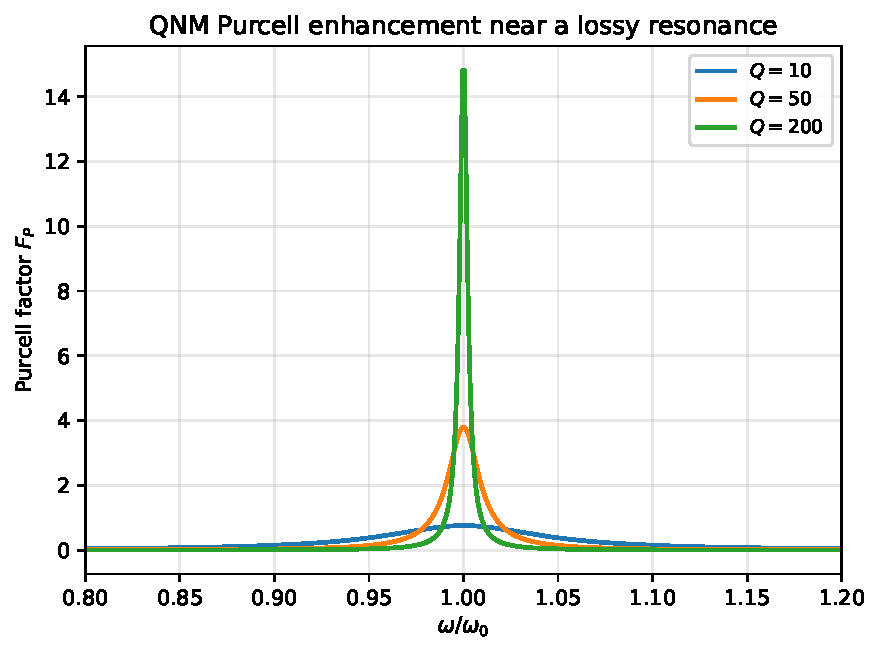
\includegraphics[width=0.6\linewidth]{figures/fig_f06_purcell_factor.pdf}
 \caption{Purcell enhancement factor $F_P(\omega)$ near a lossy
 optical resonance at $\omega_0$, computed from the QNM expansion for
 three quality factors $Q = 10$, $50$, and $200$. Higher $Q$ gives a
 taller and narrower Lorentzian peak, illustrating the trade-off
 between enhancement and bandwidth. In non-Hermitian systems, the
 Petermann factor introduces an additional correction
 (Section~\ref{sec:petermann}).}
 \label{fig:purcell-factor}
\end{figure}

\begin{takeaway}[The QNM Purcell factor]
The standard Purcell formula $F_P \propto \Qfac/V$ remains valid for open
cavities as a single-mode approximation, provided $V$ is understood as
the complex QNM mode volume and the observable rate is obtained from the
imaginary part of the Green tensor. In weakly lossy, isolated resonances
this often reduces to using $\Re\tilde{V}$ in the denominator. Using a
Hermitian, conjugated mode volume in place of the unconjugated QNM
normalization generally gives incorrect results for open or dissipative
cavities.
\end{takeaway}


%% ================================================================
\section{Perturbation theory for QNMs}
\label{sec:qnm-perturbation}

The biorthogonal framework provides a natural perturbation theory for
QNM eigenfrequencies. If the permittivity is perturbed by
$\delta\epsr(\rr)$ (e.g., by a nanoparticle binding event, a
temperature change, or a refractive-index modulation), the first-order
shift of the $n$-th QNM frequency is
\begin{equation}
 \delta\omtil_n = -\frac{\omtil_n}{2}
 \frac{\int \delta\epsr(\rr)\,\tilde{\EE}_n(\rr)\cdot\tilde{\EE}_n(\rr)\;\dd^3r}
 {\int \epsr(\rr)\,\tilde{\EE}_n(\rr)\cdot\tilde{\EE}_n(\rr)\;\dd^3r}.
 \label{eq:qnm-perturbation}
\end{equation}
This formula is the non-Hermitian analogue of the standard Rayleigh--Schr\"odinger
perturbation theory, with the unconjugated norm replacing the Hermitian
norm. Several features distinguish it from the Hermitian case:
\begin{itemize}
 \item The perturbation shift $\delta\omtil_n$ is complex: both the
 resonance frequency and the decay rate change simultaneously.
 \item The integrals involve $\tilde{\EE}_n \cdot \tilde{\EE}_n$
 (unconjugated), not $|\tilde{\EE}_n|^2$ (conjugated). For QNMs
 with large spatial divergence, these are very different.
 \item Near an exceptional point, where two QNMs coalesce, the
 denominator approaches zero and the perturbation theory breaks
 down---the response becomes $\propto\sqrt{\delta\epsr}$ rather than
 linear.
\end{itemize}

\paragraph{Example: nanoparticle sensing.}
Consider a dielectric nanoparticle of radius $a = 30\;$nm and
permittivity $\varepsilon_p = 2.25$ (silica) placed at the field maximum
of a photonic crystal cavity with $\omtil_0 = (1.22 - 0.015i) \times
10^{15}\;$rad/s ($\lambda \approx 1550\;$nm, $\Qfac \approx 40$). The
perturbation is $\delta\varepsilon = (\varepsilon_p - 1) = 1.25$ over
the nanoparticle volume $V_p = (4/3)\pi a^3 \approx 1.13 \times
10^{-22}\;$m$^3$. Using~\eqref{eq:qnm-perturbation} with a mode
volume $\tilde{V} \approx (0.8 - 0.2i)(\lambda/n)^3$ and
$\tilde{\EE}(\rr_0) \cdot \tilde{\EE}(\rr_0) \approx 1/\tilde{V}$
(from the normalization), the fractional frequency shift is
\begin{equation}
 \frac{\delta\omtil}{\omtil_0} \approx
 -\frac{\delta\varepsilon\,V_p}{2\,\varepsilon\,\tilde{V}}
 \approx -(1.4 - 0.3i) \times 10^{-4}.
 \label{eq:sensing-shift}
\end{equation}
The real part gives a resonance shift
$\delta\omega \approx -1.7 \times 10^{11}\;$rad/s ($\delta\lambda
\approx 0.22\;$nm), while the imaginary part gives a linewidth change
$\delta\gamma \approx 3.7 \times 10^{10}\;$rad/s. Both are
measurable in a standard transmission experiment. The key insight is
that the QNM perturbation theory predicts the linewidth shift as well
as the frequency shift, in contrast to Hermitian perturbation theory
which gives only the real frequency shift.


%% ================================================================
\section{Modal non-orthogonality and the Petermann factor}
\label{sec:petermann}

In a Hermitian system, the eigenmodes are orthogonal and the overlap
matrix $\langle\HH_m|\HH_n\rangle$ is diagonal. In a non-Hermitian
system, the QNMs are biorthogonal but generally not orthogonal under the
Hermitian inner product. This non-orthogonality has measurable physical
consequences.

The \emph{Petermann excess noise factor} $K_n$ for a laser mode
$\tilde{\EE}_n$ quantifies the degree of modal non-orthogonality:
\begin{equation}
 K_n = \frac{
 \langle\tilde{\EE}_n|\tilde{\EE}_n\rangle\,
 \langle\tilde{\EE}_n^{\mathrm{L}}|\tilde{\EE}_n^{\mathrm{L}}\rangle
 }{
 |\langle\tilde{\EE}_n^{\mathrm{L}}|\tilde{\EE}_n\rangle|^2
 } \ge 1.
 \label{eq:petermann}
\end{equation}
For an orthogonal (Hermitian) mode, $K_n = 1$. Near an exceptional
point, where two QNMs coalesce, $K_n$ diverges: the mode becomes
maximally non-orthogonal, and the laser linewidth is enhanced by a factor
$K_n$ above the Schawlow--Townes limit.

This connection between modal non-orthogonality, excess noise, and
exceptional points is one of the central links between the abstract
theory of non-Hermitian operators and measurable optical phenomena. It
will be revisited in Chapter~\ref{ch:exceptional-points}, where
exceptional-point sensing and noise limits are analyzed in detail.


%% ================================================================
\section{Completeness and limitations}
\label{sec:qnm-completeness}

\subsection{The completeness question}
\label{ssec:qnm-completeness-question}

The QNMs of an open system do not, by themselves, form a complete basis
in the mathematical sense~\cite{wu2024frontiers,opg2023dispersive,lasson2014roundtrip}. The full spectral decomposition includes the
continuous spectrum of radiation modes
(Section~\ref{sec:open-spectrum})~\cite{vial2014quasimodal}.

In the Green-tensor expansion~\eqref{eq:green-qnm}, the QNM sum captures
the \emph{pole} contribution to $\mathbf{G}(\omega)$. The remaining
contribution---the integral over the branch cut in the complex $\omega$
plane, which represents the continuous radiation spectrum---is missed.
This branch-cut contribution is typically small near a QNM resonance
(where the pole dominates) but can be significant far from resonance or
for broadband excitations.

\paragraph{The branch-cut integral.}
For a one-dimensional system, the Green function can be written
exactly as
\begin{equation}
 G(z, z'; \omega) = \sum_n \frac{\tilde{E}_n(z)\,\tilde{E}_n(z')}
 {2\omtil_n(\omega - \omtil_n)}
 + \frac{1}{2\pi i}\int_{\mathcal{B}}
 \frac{g(z, z'; \omega')}{\omega - \omega'}\;\dd\omega',
 \label{eq:green-complete}
\end{equation}
where the first sum is over QNM poles and the second integral is over
the branch cut $\mathcal{B}$ in the complex $\omega$ plane, which runs
along the negative imaginary axis for outgoing-wave boundary conditions.
The branch-cut integrand $g(z, z'; \omega')$ represents the contribution
of radiation modes that form a continuum rather than discrete poles.

For a high-$\Qfac$ resonator driven near a single QNM, the pole term
dominates by a factor of $\sim \Qfac$, and the branch-cut contribution
can be neglected. For broadband excitation or for frequencies between
well-separated QNMs, the branch-cut contribution provides a smooth
background that fills in the spectral gaps between resonances. The
Riesz-projection method of Wu and Lalanne~\cite{wu2026rigorous}
handles this background systematically by computing both the pole
residues and the background response from a single set of complex-frequency
simulations.

\subsection{When is a QNM expansion sufficient?}
\label{ssec:qnm-sufficiency}

The accuracy of a truncated QNM expansion depends on:
\begin{enumerate}
 \item the $\Qfac$ of the relevant modes (higher $\Qfac$ means narrower
 resonances and better QNM dominance);
 \item the spectral distance from other resonances (isolated resonances
 are better described);
 \item the spatial extent of the source or field of interest (sources
 far from the resonator couple more to radiation modes);
 \item the number of modes retained (keeping more QNMs captures
 more of the spectral response, but the branch cut is always
 missed).
\end{enumerate}

For most nanophotonic applications---Purcell enhancement, SERS,
nonlinear harmonic generation in and near a single resonator---a few-QNM
expansion is sufficient. For broadband scattering problems, a background
correction or a Riesz-projection approach is needed to capture the
non-resonant contribution~\cite{wu2026rigorous}.

\subsection{Relation to coupled-mode theory}
\label{ssec:qnm-cmt-bridge}

A QNM expansion truncated to a small number of modes is, in effect, a
\emph{coupled-mode model}: the field is represented as a superposition
of a few resonant modes, each with a complex frequency, and the dynamics
are governed by a finite-dimensional non-Hermitian matrix. The
difference from phenomenological coupled-mode theory is that the QNM
expansion is \emph{derived from Maxwell's equations} with controlled
approximations, and the coupling coefficients are determined by the
mode overlaps, not by fitting.

This connection between QNMs and effective Hamiltonians is the subject
of Chapter~\ref{ch:maxwell-coupled-modes}, where the coupled-mode
formalism is developed explicitly from the Maxwell operator.

\chapter{From Maxwell to Coupled Modes}
\label{ch:maxwell-coupled-modes}

\begin{chapterlead}
Much of non-Hermitian photonics is discussed in the language of $2\times 2$
matrices: two coupled resonances, an exceptional point where eigenvalues
coalesce, a $\PT$-symmetric Hamiltonian with balanced gain and loss.
Where do these finite-dimensional matrices come from? This chapter
answers that question by deriving coupled-mode models as controlled
reductions of the full Maxwell eigenproblem. The derivation makes
explicit what is gained and what is lost in the reduction, and establishes
the conditions under which a non-Hermitian effective Hamiltonian
faithfully represents the physics of the underlying electromagnetic system.
\end{chapterlead}


%% ================================================================
\section{Three levels of description}
\label{sec:three-levels}

Before proceeding with derivations, it is important to distinguish three
levels of electromagnetic description that are often conflated in the
literature:

\begin{enumerate}
 \item \textbf{The full Maxwell operator.} The infinite-dimensional
 operator $\Mop$ or its first-order form $\hat{\mathcal{M}}$, acting
 on the complete space of electromagnetic fields. Self-adjoint for
 lossless closed systems; non-self-adjoint when any of the three
 conditions of Chapter~\ref{ch:energy-inner} is violated.

 \item \textbf{The complete modal expansion.} A representation of the
 field as a sum over \emph{all} eigenmodes (normal modes, QNMs,
 radiation modes). This is formally exact but impractical: the sum
 involves infinitely many modes and, for open systems, the continuous
 spectrum.

 \item \textbf{The truncated effective Hamiltonian.} A finite-dimensional
 matrix $H_{\mathrm{eff}}$ acting on a small number of retained modes.
 This is the object that appears in most coupled-mode analyses.
 It is generically non-Hermitian, even when the full Maxwell operator
 is self-adjoint, because the discarded modes act as an environment.
\end{enumerate}

The passage from level~1 to level~3 is a projection. The non-Hermiticity
of $H_{\mathrm{eff}}$ arises from the projection as much as from any
intrinsic non-Hermiticity of the material or boundary conditions. This
is the fourth road to non-Hermiticity identified in
Section~\ref{ssec:road-projection}.


%% ================================================================
\section{Temporal coupled-mode theory}
\label{sec:tcmt}

\subsection{The phenomenological starting point}
\label{ssec:tcmt-phenom}

Temporal coupled-mode theory (TCMT), as introduced by Haus and later
systematized by Fan and collaborators~\cite{v2024exact,zhao2019connection}, models a set of $N$ resonant modes
coupled to $M$ input--output channels. The dynamics of the mode amplitudes
$\mathbf{a}(t) = (a_1, \ldots, a_N)^\transpose$ are governed by
\begin{equation}
 \dv{\mathbf{a}}{t}
 = \bigl(-i\boldsymbol{\Omega} - \boldsymbol{\Gamma}\bigr)\,\mathbf{a}
 + \mathbf{K}^\transpose\,\mathbf{s}_+,
 \label{eq:tcmt-time}
\end{equation}
where $\boldsymbol{\Omega}$ is the Hermitian frequency matrix,
$\boldsymbol{\Gamma}$ is the (positive semi-definite) decay-rate matrix,
$\mathbf{K}$ is the coupling matrix between modes and channels, and
$\mathbf{s}_+$ is the vector of incoming wave amplitudes. The outgoing
waves are
\begin{equation}
 \mathbf{s}_- = \mathbf{C}\,\mathbf{s}_+
 + \mathbf{K}\,\mathbf{a},
 \label{eq:tcmt-output}
\end{equation}
where $\mathbf{C}$ is the direct scattering (background) matrix.

The effective Hamiltonian is
\begin{equation}
 H_{\mathrm{eff}} = \boldsymbol{\Omega} - i\boldsymbol{\Gamma},
 \label{eq:heff-tcmt}
\end{equation}
which is manifestly non-Hermitian whenever $\boldsymbol{\Gamma} \neq 0$
(i.e., whenever the resonances have finite lifetime). The eigenvalues of
$H_{\mathrm{eff}}$ are the complex resonance frequencies $\omtil_n$; they
coincide with the QNM frequencies of the open system when the model is
accurate.

\subsection{TCMT constraints from energy conservation}
\label{ssec:tcmt-constraints}

Energy conservation and time-reversal symmetry impose algebraic
constraints on the TCMT parameters. For a lossless system with
reciprocal coupling:
\begin{align}
 \boldsymbol{\Gamma} &= \frac{1}{2}\mathbf{K}^\dagger\mathbf{K},
 \label{eq:tcmt-gamma}\\
 \mathbf{C}\mathbf{K}^* &= -\mathbf{K},
 \label{eq:tcmt-ck}
\end{align}
which together ensure that $\Smat(\omega)$ is unitary on the real axis
when material losses are absent. These constraints reduce the number of
free parameters in the TCMT model and provide self-consistency checks.

\paragraph{Derivation from energy balance.}
Constraint~\eqref{eq:tcmt-gamma} follows from requiring that the total
stored energy $W = \mathbf{a}^\dagger\mathbf{a}$ decays at a rate equal
to the total power emitted into all channels. From~\eqref{eq:tcmt-time}
with $\mathbf{s}_+ = 0$ (no input), the energy decay rate is
\begin{equation}
 \dv{W}{t} = \mathbf{a}^\dagger\dv{\mathbf{a}}{t}
 + \biggl(\dv{\mathbf{a}}{t}\biggr)^{\!\dagger}\mathbf{a}
 = -2\,\mathbf{a}^\dagger\boldsymbol{\Gamma}\,\mathbf{a}.
 \label{eq:energy-decay-rate}
\end{equation}
The power emitted into channels is
$P_{\mathrm{out}} = \mathbf{s}_-^\dagger\mathbf{s}_-
= \mathbf{a}^\dagger\mathbf{K}^\dagger\mathbf{K}\,\mathbf{a}$
(using $\mathbf{s}_+ = 0$ in~\eqref{eq:tcmt-output}).
Equating $|\dd W/\dd t| = P_{\mathrm{out}}$ for arbitrary
$\mathbf{a}$ yields~\eqref{eq:tcmt-gamma}.

Constraint~\eqref{eq:tcmt-ck} follows from time-reversal symmetry:
the time-reversed outgoing field must be a valid incoming field that
excites the time-reversed mode amplitudes. In the frequency domain,
this requires $\Smat(\omega)\Smat^*(\omega) = \mathbf{I}$ on the real
axis, which, after expanding $\Smat$ in terms of
$H_{\mathrm{eff}}$, reduces to~\eqref{eq:tcmt-ck}.

For a system with material loss or gain, the constraints are modified:
$\boldsymbol{\Gamma}$ acquires additional contributions from intrinsic
loss rates, and unitarity is replaced by a weaker bound
$\Smat^\dagger\Smat \le \mathbf{I}$ (for passive systems).

\subsection{What TCMT does not tell us}
\label{ssec:tcmt-limitations}

Equations~\eqref{eq:tcmt-time}--\eqref{eq:tcmt-output} are
phenomenological~\cite{icon2022imaginary,alpeggiani2017quasinormal,opg2021non}: they postulate a finite-dimensional linear system and
constrain its parameters by energy conservation and time-reversal
symmetry. They do not derive $\boldsymbol{\Omega}$,
$\boldsymbol{\Gamma}$, or $\mathbf{K}$ from the electromagnetic fields.
Nor do they specify which modes should be retained or how the truncation
error scales.

A Maxwell-first monograph must go further: it must connect the TCMT
parameters to the spatial field distributions and material properties of
the photonic structure. This is what the QNM-based derivation provides.


%% ================================================================
\section{Deriving the effective Hamiltonian from QNMs}
\label{sec:heff-derivation}

\subsection{Starting point: the QNM expansion}
\label{ssec:qnm-start}

Consider a photonic structure supporting $N$ well-separated QNMs
$\{\tilde{\EE}_n\}$ with complex frequencies $\{\omtil_n\}$, normalized
according to the unconjugated prescription of
Section~\ref{sec:qnm-normalization}. The Green tensor near the
resonances is (from~\eqref{eq:green-qnm})
\begin{equation}
 \mathbf{G}(\rr,\rr';\omega)
 \approx \sum_{n=1}^{N}
 \frac{c^2\,\tilde{\EE}_n(\rr)\otimes\tilde{\EE}_n(\rr')}
 {2\omtil_n(\omega - \omtil_n)}.
 \label{eq:green-few-mode}
\end{equation}

\subsection{Mode amplitudes and equations of motion}
\label{ssec:mode-amplitudes}

Expand the electric field in the vicinity of the resonator as
\begin{equation}
 \EE(\rr,t) = \sum_{n=1}^{N} a_n(t)\,\tilde{\EE}_n(\rr)
 + \EE_{\mathrm{rad}}(\rr,t),
 \label{eq:field-expansion}
\end{equation}
where $a_n(t)$ are time-dependent mode amplitudes and
$\EE_{\mathrm{rad}}$ is the contribution from the radiation continuum and
distant modes. Projecting the time-domain Maxwell equations onto the
QNM basis using the biorthogonal inner product yields, after neglecting
the continuum coupling and assuming slowly varying amplitudes,
\begin{equation}
 \dv{a_n}{t} = -i\omtil_n\,a_n - i\sum_{m\neq n} V_{nm}\,a_m
 + f_n(t),
 \label{eq:eom-amplitudes}
\end{equation}
where $V_{nm}$ is the coupling between QNMs $n$ and $m$ induced by any
perturbation (e.g., a nearby scatterer or a change in $\epsr$), and
$f_n(t)$ represents the driving by external sources.

\subsection{Mode-overlap integrals}
\label{ssec:mode-overlap}

The coupling matrix elements $V_{nm}$ are determined by mode-overlap
integrals. For a permittivity perturbation $\delta\epsr(\rr)$
(e.g., bringing two cavities into proximity), the coupling is
\begin{equation}
 V_{nm} = -\frac{\omtil_n}{2}
 \int \delta\epsr(\rr)\,\tilde{\EE}_n(\rr)\cdot\tilde{\EE}_m(\rr)
 \;\dd^3r,
 \label{eq:coupling-overlap}
\end{equation}
where the integral is over the region where $\delta\epsr \neq 0$.
This formula connects the abstract matrix element to a spatial integral
of the electromagnetic fields and the material perturbation: placing the
perturbation where both mode fields are strong maximizes the coupling.

For a reciprocal medium, Lorentz reciprocity makes the properly
normalized first-order coupling matrix complex symmetric, but not
Hermitian. Equation~\eqref{eq:coupling-overlap} is a compact scalar
perturbation formula; when the frequencies of the two modes differ
substantially, the prefactor and normalization must be treated with care.
Near a degenerate pair it is common to use a symmetrized reference
frequency, giving $V_{nm}=V_{mn}$ to the same perturbative order. The
important point is that reciprocity implies transpose symmetry, not
complex-conjugate symmetry.

\subsection{The effective Hamiltonian}
\label{ssec:heff-matrix}

In matrix form, the homogeneous part of~\eqref{eq:eom-amplitudes} is
\begin{equation}
 i\,\dv{\mathbf{a}}{t} = H_{\mathrm{eff}}\,\mathbf{a},
 \qquad
 (H_{\mathrm{eff}})_{nm} = \omtil_n\,\delta_{nm} + V_{nm}.
 \label{eq:heff-matrix}
\end{equation}
This is a non-Hermitian matrix whose diagonal entries are the complex QNM
frequencies and whose off-diagonal entries are the inter-mode couplings.
It is the Maxwell-derived counterpart of the phenomenological
$H_{\mathrm{eff}} = \boldsymbol{\Omega} - i\boldsymbol{\Gamma}$ from
TCMT, with the crucial advantage that every matrix element is determined
by the electromagnetic fields and material properties.

\begin{takeaway}[From Maxwell to matrix]
The non-Hermitian effective Hamiltonian of coupled-mode theory is not a
postulate---it is a controlled approximation to the full Maxwell
eigenproblem, obtained by expanding in QNMs and projecting out the
radiation continuum. Its non-Hermiticity has two sources: the intrinsic
complex frequencies of the QNMs (from radiation or absorption) and the
truncation of the modal basis.
\end{takeaway}


%% ================================================================
\section{Example: two coupled cavities}
\label{sec:two-cavity-example}

Consider two identical photonic crystal cavities, each supporting a
single QNM at complex frequency $\omtil_0 = \omega_0 - i\gamma_0$,
separated by a barrier of $N_b$ lattice periods.

\subsection{Isolated-cavity QNMs}
\label{ssec:isolated-cavities}

Each isolated cavity has a QNM field $\tilde{\EE}_0(\rr)$ that decays
evanescently into the barrier as $\exp(-\kappa_{\mathrm{gap}}x)$, with
characteristic length $\ell_{\mathrm{ev}} = 1/\kappa_{\mathrm{gap}}$.
Here $\kappa_{\mathrm{gap}}$ is the evanescent decay constant at the gap
frequency and $a$ is the lattice period.

When the cavities are brought to a separation $d = N_b a$, the field
of cavity~1 has a small but nonzero amplitude at the location of
cavity~2, and vice versa. The perturbation is the presence of the
other cavity, described by $\delta\epsr(\rr)$ in the region of
cavity~2.

\subsection{Coupling strength}
\label{ssec:coupling-strength}

The coupling matrix element~\eqref{eq:coupling-overlap} gives
\begin{equation}
 V_{12} = -\frac{\omtil_0}{2}
 \int_{\mathrm{cav\,2}} \delta\epsr(\rr)\,
 \tilde{\EE}_1(\rr)\cdot\tilde{\EE}_2(\rr)\;\dd^3r
 \approx \kappa_0\,e^{-\kappa_{\mathrm{gap}} d},
 \label{eq:two-cavity-coupling}
\end{equation}
where $\kappa_0$ is a prefactor determined by the QNM field profiles and
the dielectric contrast. The exponential dependence on the
barrier thickness $d$ is the signature of evanescent coupling.

For a typical silicon photonic crystal cavity at $\lambda = 1550\;\mathrm{nm}$
with $Q_0 = 10^4$ and $N_b = 3$ barrier periods, the coupling can be
$\kappa \sim 10^{11}\;\mathrm{rad/s}$, much larger than the decay rate
$\gamma_0 = \omega_0/(2Q_0) \sim 6 \times 10^{10}\;\mathrm{rad/s}$. In
this regime, the modes hybridize strongly, producing a symmetric and an
antisymmetric supermode with frequency splitting $2\kappa$.

\paragraph{Quantitative example.}
For concreteness, take a one-dimensional photonic crystal of GaAs
($\varepsilon = 12.25$) and air with period $a = 350\;$nm, supporting
a defect cavity at $\lambda_0 = 1550\;$nm with $Q_0 = 8000$. Then
$\omega_0 = 2\pi c/\lambda_0 \approx 1.215 \times 10^{15}\;$rad/s,
$\gamma_0 = \omega_0/(2Q_0) \approx 7.6 \times 10^{10}\;$rad/s.
With $N_b = 4$ barrier periods and an evanescent decay constant
$\kappa_{\mathrm{gap}}\,a \approx 1.2$, the inter-cavity coupling is
$\kappa \approx \kappa_0\,e^{-4 \times 1.2} \approx 8.3 \times 10^{-3}\,\kappa_0$.
For $\kappa_0 \sim 5 \times 10^{13}\;$rad/s (estimated from the
mode-overlap integral), this gives
$\kappa \approx 4.2 \times 10^{11}\;$rad/s, so
$\kappa/\gamma_0 \approx 5.5$: the system is in the strong-coupling
regime. The supermode splitting is $2\kappa \approx 8.4 \times
10^{11}\;$rad/s, corresponding to a wavelength splitting
$\Delta\lambda \approx \lambda_0^2\,\kappa/(\pi c) \approx 1.1\;$nm.
This splitting is easily resolvable in a standard optical spectrum
analyser, confirming that the two-mode Hamiltonian makes a testable
prediction.

Reducing the barrier to $N_b = 2$ increases $\kappa$ by a factor
$e^{2 \times 1.2} \approx 11$, bringing $\kappa/\gamma_0 \approx 60$:
the modes are deeply hybridized and the splitting dominates the
linewidth. Increasing the barrier to $N_b = 6$ reduces $\kappa$ below
$\gamma_0$, placing the system in the weak-coupling regime where the
supermode splitting is unresolved and the two resonances merge into a
single broadened peak.

\subsection{The two-mode Hamiltonian}
\label{ssec:two-mode-hamiltonian}

The effective Hamiltonian for the two-cavity system is
\begin{equation}
 H_{\mathrm{eff}} = \begin{pmatrix}
 \omtil_0 & V_{12} \\
 V_{21} & \omtil_0
 \end{pmatrix}
 = \omega_0 \mathbf{I} - i\gamma_0 \mathbf{I}
 + \begin{pmatrix} 0 & \kappa \\ \kappa & 0 \end{pmatrix},
 \label{eq:two-cavity-heff}
\end{equation}
where $\kappa = V_{12} = V_{21}$ (reciprocity) and $\kappa$ is real to
lowest order in the evanescent overlap. The eigenvalues are
$\omtil_\pm = \omega_0 - i\gamma_0 \pm \kappa$: two real-split modes
with the same decay rate.

If the two cavities are made non-identical---one with additional gain
and the other with additional loss---the diagonal entries become
$\omtil_0 \pm i\gamma_{\mathrm{gl}}$, and the Hamiltonian is the
$\PT$-symmetric model of Chapter~\ref{ch:pt-symmetric} with a
Maxwell-derived coupling $\kappa$.

\begin{figure}[t]
 \centering
 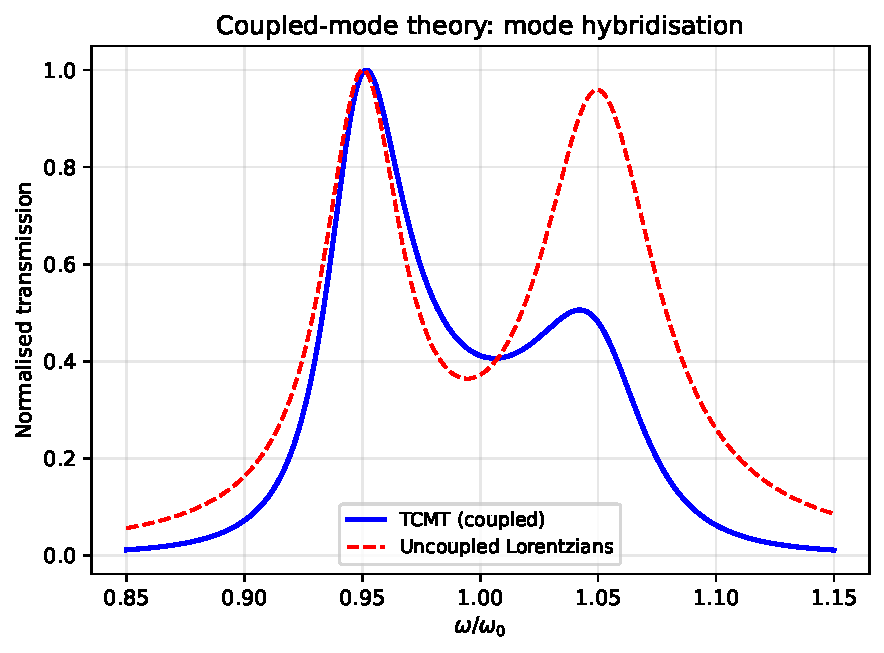
\includegraphics[width=0.68\linewidth]{figures/fig_f07_reaction_cmt.pdf}
 \caption{Coupled-mode hybridisation in a two-resonator system. The
 TCMT prediction (blue) shows the splitting produced by coherent
 inter-cavity coupling, while the uncoupled Lorentzian estimate (red
 dashed) misses the hybridised supermodes. The comparison emphasizes
 why the reaction and QNM-overlap derivations are needed: coupling is
 not a phenomenological fitting parameter but a Maxwell overlap integral
 between open resonator fields.}
 \label{fig:reaction-cmt}
\end{figure}


%% ================================================================
\section{The reaction inner product}
\label{sec:reaction}

An alternative derivation of coupled-mode equations, developed by Xu and
Chen~\cite{xu2015general}, uses the concept of \emph{reaction} from
electromagnetic theory. The reaction of a field $(\EE_a, \HH_a)$ on a
source $\JJ_b$ is
\begin{equation}
 \langle a, b\rangle_{\mathrm{R}}
 = \int \EE_a\cdot\JJ_b\;\dd^3 r,
 \label{eq:reaction-def}
\end{equation}
which is an unconjugated bilinear form---the same structure as the QNM
normalization of Section~\ref{sec:qnm-normalization}.

\subsection{Reciprocity and the symmetric coupling}
\label{ssec:reaction-reciprocity}

For a reciprocal medium, the Lorentz reciprocity theorem
(Section~\ref{sec:reciprocity}) ensures that
$\langle a, b\rangle_{\mathrm{R}} = \langle b, a\rangle_{\mathrm{R}}$:
the reaction is symmetric. This symmetry is the foundation for a
\emph{generalized coupled-mode theory} (GCMT) that works in non-Hermitian
waveguides, where the standard power-conservation-based CMT
fails~\cite{xu2015general}.

The GCMT replaces the Hermitian power inner product
$\langle\EE_a^*,\EE_b\rangle$ with the reaction inner product
$\langle\EE_a,\EE_b\rangle_{\mathrm{R}}$ (no conjugation), and derives
coupled-mode equations that remain valid even in $\PT$-symmetric and
gain--loss waveguides. The resulting coupling matrix is symmetric
(by reciprocity) but not Hermitian---precisely the structure expected for
a non-Hermitian system that is still reciprocal.

\subsection{Connection to QNM biorthogonality}
\label{ssec:reaction-qnm}

The reaction inner product and the QNM biorthogonal inner product are
closely related. For two QNMs of the same structure, the biorthogonality
relation~\eqref{eq:biorthogonality} can be rewritten as a vanishing
reaction:
\begin{equation}
 \langle\tilde{\EE}_m,\,\epsr\tilde{\EE}_n\rangle_{\mathrm{R}}
 = \int \epsr(\rr)\,\tilde{\EE}_m(\rr)\cdot\tilde{\EE}_n(\rr)\;\dd^3r
 = 0
 \qquad (m \neq n).
 \label{eq:reaction-biorthogonal}
\end{equation}
This confirms that the QNM-based and reaction-based derivations of
coupled-mode theory are different presentations of the same underlying
structure: both use unconjugated bilinear forms enforced by reciprocity.

\subsection{When reaction-CMT and TCMT disagree}
\label{ssec:reaction-tcmt-disagree}

For Hermitian waveguides, the reaction inner product and the standard
power-orthogonality inner product give equivalent coupled-mode
equations. However, for non-Hermitian waveguides with gain or loss,
the two approaches can give \emph{different} coupling coefficients.
The standard power-based CMT assumes $\langle\EE_a^*,\EE_b\rangle$ is
the correct overlap, which is valid only when the modes carry positive
definite power. In a gain--loss waveguide, some modes can carry
negative power (the field does work on the medium rather than the
reverse), and the power-orthogonality assumption fails.

The reaction-based CMT avoids this problem because the reaction inner
product does not involve complex conjugation and does not require
positive definiteness. It is therefore the correct starting point for
deriving coupled-mode equations in $\PT$-symmetric waveguides, gain
waveguides, and any system where the modes are not power-orthogonal.

The practical consequence is that the reaction-CMT coupling coefficient
between a gain mode and a loss mode can be purely imaginary, even when
the waveguides are identical except for the sign of the imaginary part
of $\varepsilon$. This imaginary coupling is responsible for the
$\PT$ phase transition in coupled waveguides: below the transition
the coupling compensates the gain--loss imbalance, and above it the
eigenvalues become complex conjugate pairs.


%% ================================================================
\section{Two coupled resonances: the minimal model}
\label{sec:two-mode}

The simplest and most frequently used non-Hermitian model in photonics
is a pair of coupled resonances described by the $2\times 2$ matrix
\begin{equation}
 H_{\mathrm{eff}} =
 \begin{pmatrix}
 \omega_1 - i\gamma_1 & \kappa \\
 \kappa & \omega_2 - i\gamma_2
 \end{pmatrix},
 \label{eq:two-mode-H}
\end{equation}
where $\omega_j$ are the bare resonant frequencies, $\gamma_j$ the decay
rates, and $\kappa$ the coupling strength (real for a reciprocal system
without radiation coupling corrections).

The eigenvalues are
\begin{equation}
 \omtil_\pm = \bar{\omega} - i\bar{\gamma}
 \pm \sqrt{\left(\frac{\Delta\omega - i\Delta\gamma}{2}\right)^2
 + \kappa^2},
 \label{eq:two-mode-evals}
\end{equation}
where $\bar{\omega} = (\omega_1+\omega_2)/2$,
$\bar{\gamma} = (\gamma_1+\gamma_2)/2$,
$\Delta\omega = \omega_1 - \omega_2$, and
$\Delta\gamma = \gamma_1 - \gamma_2$.

When $\Delta\omega = 0$ (degenerate bare frequencies), the eigenvalues
become
\begin{equation}
 \omtil_\pm = \bar{\omega} - i\bar{\gamma}
 \pm \sqrt{\kappa^2 - \left(\frac{\Delta\gamma}{2}\right)^2}.
 \label{eq:two-mode-ep}
\end{equation}
An \emph{exceptional point} occurs when the square root vanishes:
$\kappa = |\Delta\gamma|/2$. At this point, not only the eigenvalues but
also the eigenvectors coalesce, and the matrix becomes defective (its
Jordan normal form contains a $2\times 2$ Jordan block). This is the
subject of Chapter~\ref{ch:exceptional-points}.


%% ================================================================
\section{Validity and breakdown}
\label{sec:cmt-validity}

The effective Hamiltonian~\eqref{eq:heff-matrix} is a useful and often
accurate model, but it is an approximation. Its validity requires:

\begin{enumerate}
 \item \textbf{Mode isolation.} The retained QNMs must be spectrally
 well separated from all other resonances and from the continuum
 threshold. Overlapping resonances require more modes or a different
 approach.

 \item \textbf{Weak perturbation.} The coupling $V_{nm}$ should be
 small compared to the frequency separation between modes, so that the
 perturbative projection is accurate.

 \item \textbf{Narrow bandwidth.} The driving field should have a
 bandwidth smaller than the free spectral range, so that only the
 retained modes are significantly excited.

 \item \textbf{Linearity.} The expansion assumes linear media. Near
 and above the lasing threshold, gain saturation introduces nonlinear
 corrections that are not captured by a linear $H_{\mathrm{eff}}$.
\end{enumerate}

When these conditions break down, the effective Hamiltonian picture fails
and one must return to the full Maxwell operator---either numerically or
through a more complete modal expansion. The practical question is not
whether a truncated model is ever exact, but whether the neglected modes
are far enough away that their effect can be treated perturbatively. A
clean way to express this is the Schur complement: partition the complete
modal Hamiltonian into retained modes $P$ and eliminated modes $Q$,
\begin{equation}
 H = \begin{pmatrix} H_{PP} & H_{PQ} \\
 H_{QP} & H_{QQ} \end{pmatrix}.
 \label{eq:schur-partition}
\end{equation}
Eliminating the $Q$ subspace gives the frequency-dependent effective
operator
\begin{equation}
 H_{\mathrm{eff}}(\omega)
 = H_{PP} + H_{PQ}\,(\omega - H_{QQ})^{-1}H_{QP}.
 \label{eq:schur-heff}
\end{equation}
The naive truncation keeps only $H_{PP}$. It is accurate only when
$\|H_{PQ}\|^2/\Delta$ is small, where $\Delta$ is the spectral separation
between the retained and eliminated modes. The Schur-complement
correction is second-order in $H_{PQ}$ and first-order in $1/\Delta$:
it systematically improves the naive truncation by accounting for the
virtual excitation of the eliminated modes.  The truncation is accurate
when the coupling-to-detuning ratio $\|H_{PQ}\|/\Delta$ is small;
the leading correction scales as $\|H_{PQ}\|^2/\Delta$.

\paragraph{Convergence with spectral separation.}
For the four-mode test model used in Figure~\ref{fig:qnm-cmt-truncation},
the naive two-mode truncation error (the maximum eigenvalue error
relative to the four-mode reference) is $\sim 1.1 \times 10^{-2}$ when
the eliminated modes are $5\gamma$ away, and decreases to
$\sim 8.5 \times 10^{-4}$ at $10\gamma$ separation. Including the
Schur-complement correction reduces these errors to
$\sim 4.8 \times 10^{-3}$ and $\sim 5.9 \times 10^{-5}$, respectively.
The leading Schur correction scales as $\|H_{PQ}\|^2/\Delta$,
so the residual error after correction is of order
$\|H_{PQ}\|^3/\Delta^2$---one power higher than the naive
truncation error.  This is why the green curves in
Figure~\ref{fig:qnm-cmt-truncation} converge much faster with
increasing spectral separation.

The practical lesson is clear: a two-mode model is adequate when the
nearest unretained resonance is more than $\sim 10$ linewidths away.
For denser spectra, more modes must be retained or the Schur complement
must be applied. This criterion directly impacts the design of
non-Hermitian photonic devices: a PT-symmetric laser operating near
an exceptional point is sensitive to distant modes precisely when the
Schur-complement correction becomes large.

\paragraph{Example: three-mode reduction to a two-mode
$\PT$-symmetric Hamiltonian.}
Consider three QNMs with complex frequencies
$\tilde{\omega}_1 = \omega_0 + i\gamma$,
$\tilde{\omega}_2 = \omega_0 - i\gamma$, and
$\tilde{\omega}_3 = \omega_0 + \Delta - i\gamma_3$, where
$\Delta \gg \gamma, \gamma_3$ is the detuning of the third mode from the
near-degenerate pair. Modes~1 and~2 form a gain--loss pair (balanced
when their real frequencies coincide and their imaginary parts are
opposite), while mode~3 is a distant lossy resonance. The
full $3\times 3$ Hamiltonian is
\begin{equation}
 H = \begin{pmatrix}
 \omega_0 + i\gamma & \kappa_{12} & \kappa_{13} \\
 \kappa_{12} & \omega_0 - i\gamma & \kappa_{23} \\
 \kappa_{13} & \kappa_{23} & \omega_0 + \Delta - i\gamma_3
 \end{pmatrix},
 \label{eq:three-mode-full}
\end{equation}
where $\kappa_{ij}$ are inter-mode couplings from the reaction inner
product~\eqref{eq:reaction-def}; in this example they are taken real,
so the matrix is real-symmetric apart from the diagonal gain/loss
terms.  We treat modes~1 and~2 as the
retained subspace $P$ and mode~3 as the eliminated subspace $Q$, so
\begin{equation}
 H_{PP} = \begin{pmatrix}
 \omega_0 + i\gamma & \kappa_{12} \\
 \kappa_{12} & \omega_0 - i\gamma
 \end{pmatrix}, \quad
 H_{PQ} = \begin{pmatrix} \kappa_{13} \\ \kappa_{23} \end{pmatrix},
 \quad H_{QQ} = \omega_0 + \Delta - i\gamma_3.
 \label{eq:three-mode-partition}
\end{equation}
The Schur complement~\eqref{eq:schur-heff} gives
\begin{equation}
 H_{\mathrm{eff}}(\omega) = H_{PP}
 + \frac{1}{\omega - \omega_0 - \Delta + i\gamma_3}
 \begin{pmatrix}
   \kappa_{13}^2 & \kappa_{13}\kappa_{23} \\
   \kappa_{13}\kappa_{23} & \kappa_{23}^2
 \end{pmatrix}.
 \label{eq:three-mode-schur}
\end{equation}
Evaluating at $\omega \approx \omega_0$ (near the retained pair) and
expanding to leading order in $1/\Delta$:
\begin{equation}
 H_{\mathrm{eff}} \approx
 \begin{pmatrix}
   \omega_0 + i\gamma - \frac{\kappa_{13}^2}{\Delta} &
   \kappa_{12} - \frac{\kappa_{13}\kappa_{23}}{\Delta} \\[6pt]
   \kappa_{12} - \frac{\kappa_{13}\kappa_{23}}{\Delta} &
   \omega_0 - i\gamma - \frac{\kappa_{23}^2}{\Delta}
 \end{pmatrix}.
 \label{eq:three-mode-effective}
\end{equation}
The distant mode has three effects.  First, it shifts both frequencies
downward by $\kappa_{j3}^2/\Delta$ for $j = 1,2$ (a repulsive level
shift familiar from second-order perturbation theory, with generally
different magnitudes for the two retained modes).  Second, it renormalises the
coupling: the effective coupling becomes
$\kappa_{\mathrm{eff}} = \kappa_{12} - \kappa_{13}\kappa_{23}/\Delta$,
which can either strengthen or weaken the hybridisation depending on
the sign of $\kappa_{13}\kappa_{23}$. Third, the small imaginary part of
the denominator adds loss corrections; when $\kappa_{13}$ and
$\kappa_{23}$ are unequal, both the level shifts and the induced losses
are different for the two retained modes. This is a Maxwell-derived
mechanism by which a distant spectator mode can lift the $\PT$ symmetry
of a nominally balanced gain--loss pair---an effect invisible to the
naive two-mode truncation.

\paragraph{Quantitative estimate.}
For the parameters $\omega_0 = 1$, $\gamma = 0.05$, $\Delta = 0.5$,
$\kappa_{12} = 0.03$, $\kappa_{13} = 0.02$, $\kappa_{23} = 0.01$,
and $\gamma_3 = 0.02$, the naive two-mode model predicts an EP at
$\gamma_{\mathrm{EP}} = \kappa_{12} = 0.03$. The Schur-corrected
model shifts this to
$\gamma_{\mathrm{EP}} = |\kappa_{\mathrm{eff}}| = |0.03 - 0.02 \times 0.01/0.5| = 0.0296$
and introduces a $\PT$-breaking detuning of
$(\kappa_{13}^2 - \kappa_{23}^2)/\Delta = (4 \times 10^{-4} - 1 \times 10^{-4})/0.5 = 6 \times 10^{-4}$.
For this relatively isolated pair, the corrections are small
($\sim 1\%$). But as $\Delta$ decreases toward $5\gamma = 0.25$, the
corrections grow to $\sim 4\%$ in coupling and $\sim 2.4 \times 10^{-3}$
in detuning---large enough to shift the EP position measurably in
experiments that probe the eigenvalue splitting with sub-linewidth
resolution.

\begin{figure}[t]
 \centering
 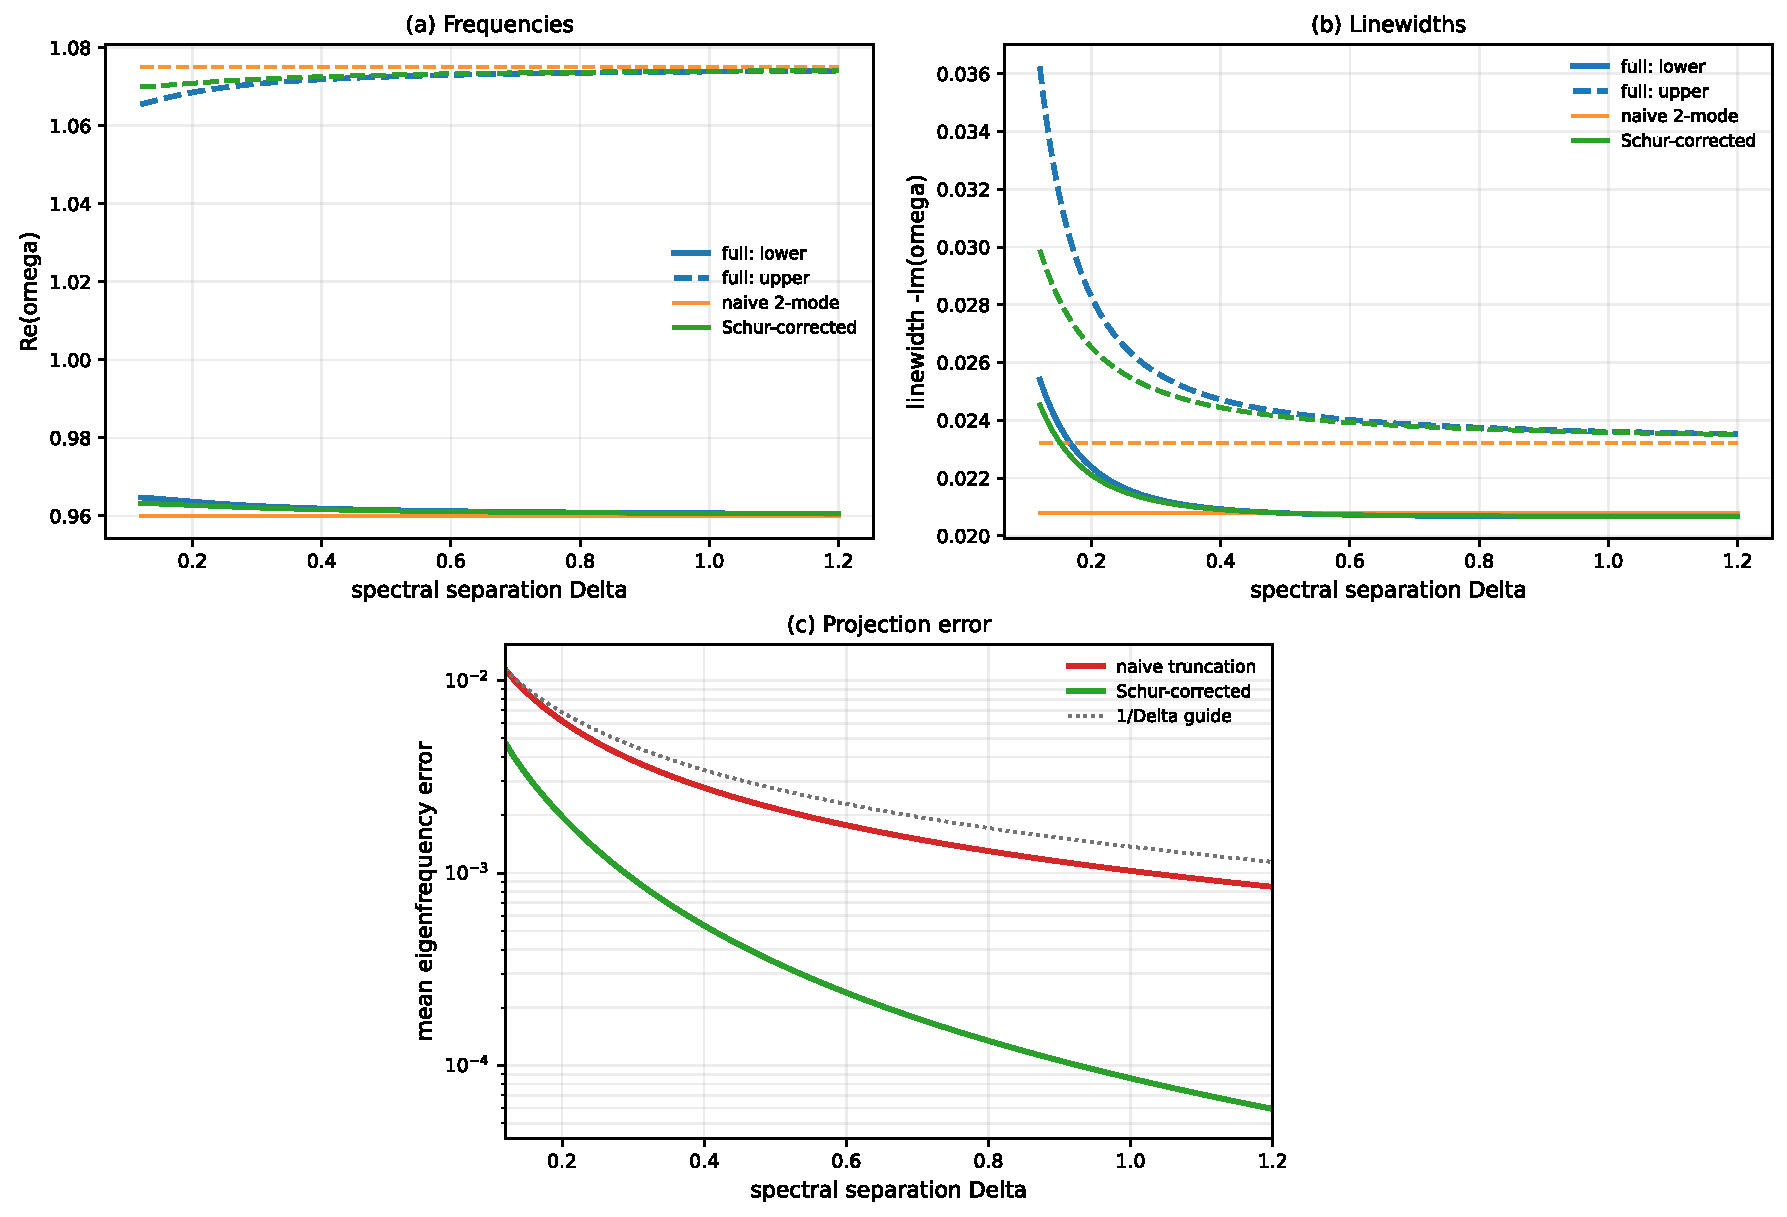
\includegraphics[width=0.98\textwidth]{fig_f7_modal_truncation.pdf}
 \caption{Controlled reduction from a larger QNM modal space to a
 two-mode coupled-mode Hamiltonian. A four-mode non-Hermitian modal
 model is treated as the ``full'' modal expansion; two near-resonant
 modes are retained while two distant modes are eliminated. The naive
 two-mode truncation captures the qualitative splitting but misses
 linewidth and frequency shifts from the eliminated modes. A
 Schur-complement correction greatly reduces the error, especially when
 the eliminated modes are spectrally separated.}
 \label{fig:qnm-cmt-truncation}
\end{figure}


%% ================================================================
\section{Beyond two modes}
\label{sec:beyond-two}

\subsection{Multi-mode effective Hamiltonians}
\label{ssec:multi-mode}

For systems with more than two relevant QNMs, the effective Hamiltonian
is an $N\times N$ non-Hermitian matrix with entries determined by the
QNM frequencies and mode-overlap integrals. The structure of this matrix
reflects the symmetries of the photonic system:
\begin{itemize}
 \item \textbf{Reciprocity:} the coupling matrix $V_{nm}$ is symmetric
 ($V_{nm} = V_{mn}$), but not Hermitian.
 \item \textbf{$\PT$ symmetry:} if the permittivity satisfies
 $\epsr(\rr) = \epsr^*(-\rr)$, the effective Hamiltonian commutes
 with the $\PT$ operator, constraining its eigenvalue structure.
 \item \textbf{Rotation symmetry:} if the structure has $C_n$
 rotational symmetry, the QNMs can be labeled by angular momentum
 quantum numbers, and the Hamiltonian block-diagonalizes.
\end{itemize}

\paragraph{From coupled cavities to tight-binding photonics.}
When the photonic structure is a periodic lattice of identical cavities,
each supporting a single QNM at $\omtil_0$, the multi-mode effective
Hamiltonian becomes a tight-binding matrix:
\begin{equation}
 (H_{\mathrm{eff}})_{nm} = \omtil_0\,\delta_{nm}
 + \kappa_{nm}\,(1 - \delta_{nm}),
 \label{eq:tight-binding-photonic}
\end{equation}
where $\kappa_{nm}$ is the evanescent coupling between sites $n$ and $m$,
determined by the mode-overlap integral~\eqref{eq:coupling-overlap}. For
nearest-neighbour coupling only, $\kappa_{nm} = \kappa\,(\delta_{n,m+1} +
\delta_{n,m-1})$, and the dispersion relation is
$\omtil(\kk) = \omtil_0 + 2\kappa\cos(k\,a)$---the photonic analogue of
the electronic tight-binding band. This is the starting point for the
Su--Schrieffer--Heeger (SSH) model of Chapter~\ref{ch:complex-bands},
where alternating coupling strengths $\kappa_1 \neq \kappa_2$ produce a
topological band gap, and for the Hatano--Nelson model of
Chapter~\ref{ch:skin-effect}, where asymmetric couplings
$\kappa_L \neq \kappa_R$ require non-reciprocal elements, synthetic
gauge bias, or reservoir-engineered dissipative couplings rather than
ordinary reciprocal gain and loss alone. The crucial point is that all
these tight-binding models have a Maxwell-first origin through the QNM
mode-overlap integrals derived in this chapter.

\subsection{From coupled modes to scattering matrix}
\label{ssec:cmt-to-smatrix}

The TCMT output relation~\eqref{eq:tcmt-output} connects the effective
Hamiltonian to the full scattering matrix. In the frequency domain,
the scattering matrix is
\begin{equation}
 \Smat(\omega) = \mathbf{C} - i\mathbf{K}\,
 (\omega\mathbf{I} - H_{\mathrm{eff}})^{-1}\,\mathbf{K}^\transpose,
 \label{eq:smat-from-heff}
\end{equation}
where the poles of $\Smat$ are the eigenvalues of $H_{\mathrm{eff}}$
and the residues are determined by the coupling to the channels. This
formula provides the bridge between the effective Hamiltonian
(Chapters~\ref{ch:exceptional-points}--\ref{ch:pt-symmetric}) and the
pole--zero scattering theory (Chapter~\ref{ch:poles-zeros}).

\begin{figure}[t]
 \centering
 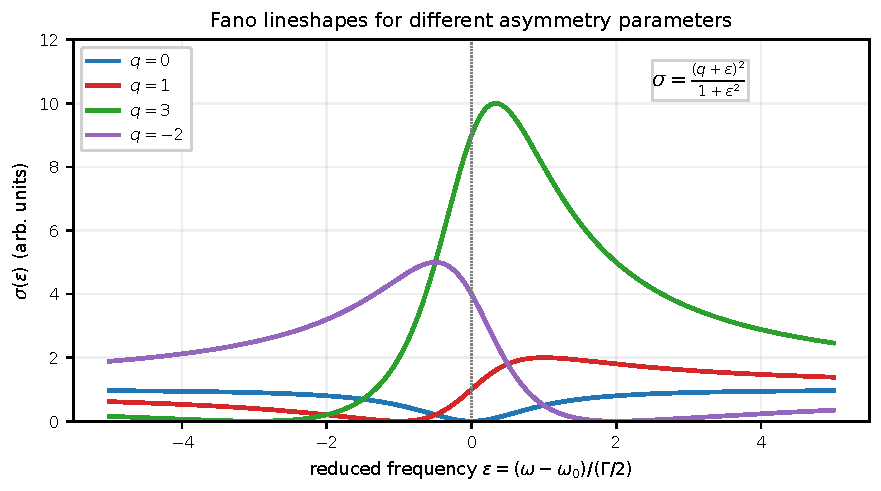
\includegraphics[width=0.62\linewidth]{fig_f7_fano.pdf}
 \caption{Fano lineshapes for different asymmetry parameters~$q$.
 The Fano formula
 $\sigma(\varepsilon) = (q + \varepsilon)^2/(1 + \varepsilon^2)$,
 where $\varepsilon = (\omega - \omega_0)/(\Gamma/2)$ is the reduced
 frequency, gives a symmetric antiresonance for $q=0$ and approaches a
 Lorentzian peak only in the large-$|q|$ limit after normalization.
 Finite positive and negative $q$ values produce asymmetric peak--dip
 profiles on opposite sides of the resonance. The asymmetry arises from
 interference between a discrete resonance and a continuum pathway---
 precisely the structure captured by the TCMT scattering
 matrix~\eqref{eq:smat-from-heff}. The dotted line marks zero detuning.}
 \label{fig:fano-lineshapes}
\end{figure}


\begin{remark}
The widespread use of $2\times 2$ models in non-Hermitian photonics is
both a strength and a danger. The models are analytically tractable and
capture essential physics (exceptional points, $\PT$ transitions, mode
coalescence), but they can also mislead when applied outside their domain
of validity. Throughout this book, we will use effective Hamiltonians
as tools for understanding, while always checking their predictions
against the full Maxwell theory whenever quantitative accuracy is needed.
\end{remark}


% ════════════════════════════════════════════════════════════
% PART III — Exceptional Photonics and Non-Hermitian Scattering
% ════════════════════════════════════════════════════════════
\part{Exceptional Photonics and Non-Hermitian Scattering}

\chapter{Exceptional Points}
\label{ch:exceptional-points}

\begin{chapterlead}
In Hermitian physics, degeneracies are points where eigenvalues coincide
but eigenvectors remain independent. Non-Hermitian operators admit a
different type of degeneracy: the \emph{exceptional point}, where both
eigenvalues \emph{and} eigenvectors coalesce. The operator becomes
defective---it cannot be diagonalized---and the response of the system
changes qualitatively. Exceptional points are not mathematical
curiosities; they have been observed in optical microcavities, coupled
waveguides, microwave billiards, and phononic crystals, and they underlie
proposals for enhanced sensing, unidirectional lasing, and topological
mode switching. The theory of exceptional points is developed from the
non-Hermitian matrix formalism of
Chapter~\ref{ch:maxwell-coupled-modes} and connects it to measurable
electromagnetic phenomena.
\end{chapterlead}


%% ================================================================
\section{Degeneracy versus defectiveness}
\label{sec:deg-vs-defect}

In a Hermitian operator, two eigenvalues can coincide at a
\emph{diabolic point} (a degeneracy). The eigenspace is two-dimensional:
two linearly independent eigenvectors exist, and the operator can still
be diagonalized. Perturbations generically split the degeneracy
linearly.

A non-Hermitian operator allows a different kind of
degeneracy. At an \emph{exceptional point} (EP), two (or more)
eigenvalues coalesce \emph{and the corresponding eigenvectors collapse
onto a single direction}. The eigenspace is one-dimensional, the
algebraic multiplicity exceeds the geometric multiplicity, and the
operator cannot be diagonalized. Instead, its Jordan normal form
contains an off-diagonal block.

\begin{definition}[Exceptional point of order $n$]
An exceptional point of order $n$ (EP$_n$)~\cite{bergholtz2019exceptional,zhen2015spawning,al2019exceptional} is a point in parameter space
where $n$ eigenvalues and $n$ eigenvectors simultaneously coalesce.
The Jordan block is $n\times n$. The most common case is EP$_2$;
higher-order exceptional points (EP$_3$, EP$_4$, \ldots) require
fine-tuning of additional parameters~\cite{kawabata2019classification,wiersig2023petermann}.
\end{definition}

\subsection{Codimension counting}
\label{ssec:codimension}

An EP$_2$ requires two real conditions (one for the real part and one for
the imaginary part of the discriminant to vanish). In a two-real-parameter
space, an EP$_2$ is therefore generically an isolated point. In a
three-parameter space, EP$_2$s form curves; in higher-dimensional
parameter spaces they form surfaces or manifolds. This codimension
argument explains why EP$_2$s are ubiquitous in two-parameter photonic
systems (e.g., coupled cavities tuned by coupling strength and gain--loss
contrast) but require no fine-tuning beyond what the experimental setup
naturally provides.

An EP$_n$ has codimension $2(n-1)$: it requires $2(n-1)$ real parameters
to be simultaneously tuned. This is why EP$_3$ and higher are
progressively more difficult to realize.


%% ================================================================
\section{The $2\times 2$ exceptional point}
\label{sec:ep2}

\subsection{Eigenvalue structure}
\label{ssec:ep2-eigenvalues}

Consider the generic two-mode effective Hamiltonian from
Section~\ref{sec:two-mode}:
\begin{equation}
 H =
 \begin{pmatrix}
 \omega_0 + \delta & \kappa \\
 \kappa & \omega_0 - \delta
 \end{pmatrix},
 \label{eq:ep-H}
\end{equation}
where $\omega_0$ is the mean frequency, $\delta$ is a complex detuning
parameter, and $\kappa$ is the coupling. The eigenvalues are
\begin{equation}
 \omtil_\pm = \omega_0 \pm \sqrt{\delta^2 + \kappa^2}.
 \label{eq:ep-evals}
\end{equation}

An exceptional point occurs when the discriminant vanishes:
\begin{equation}
 \delta^2 + \kappa^2 = 0
 \qquad\Longrightarrow\qquad
 \delta = \pm i\kappa.
 \label{eq:ep-condition}
\end{equation}
Since $\delta$ is in general complex, the EP condition is satisfied at
isolated points in the space of system parameters.

For the physically important case where $\delta$ parameterizes the
gain--loss contrast (purely imaginary: $\delta = i\gamma$) and $\kappa$
is a real coupling, the EP condition becomes $\gamma = \pm\kappa$: the
gain--loss contrast equals the coupling strength.

\begin{figure}[t]
 \centering
 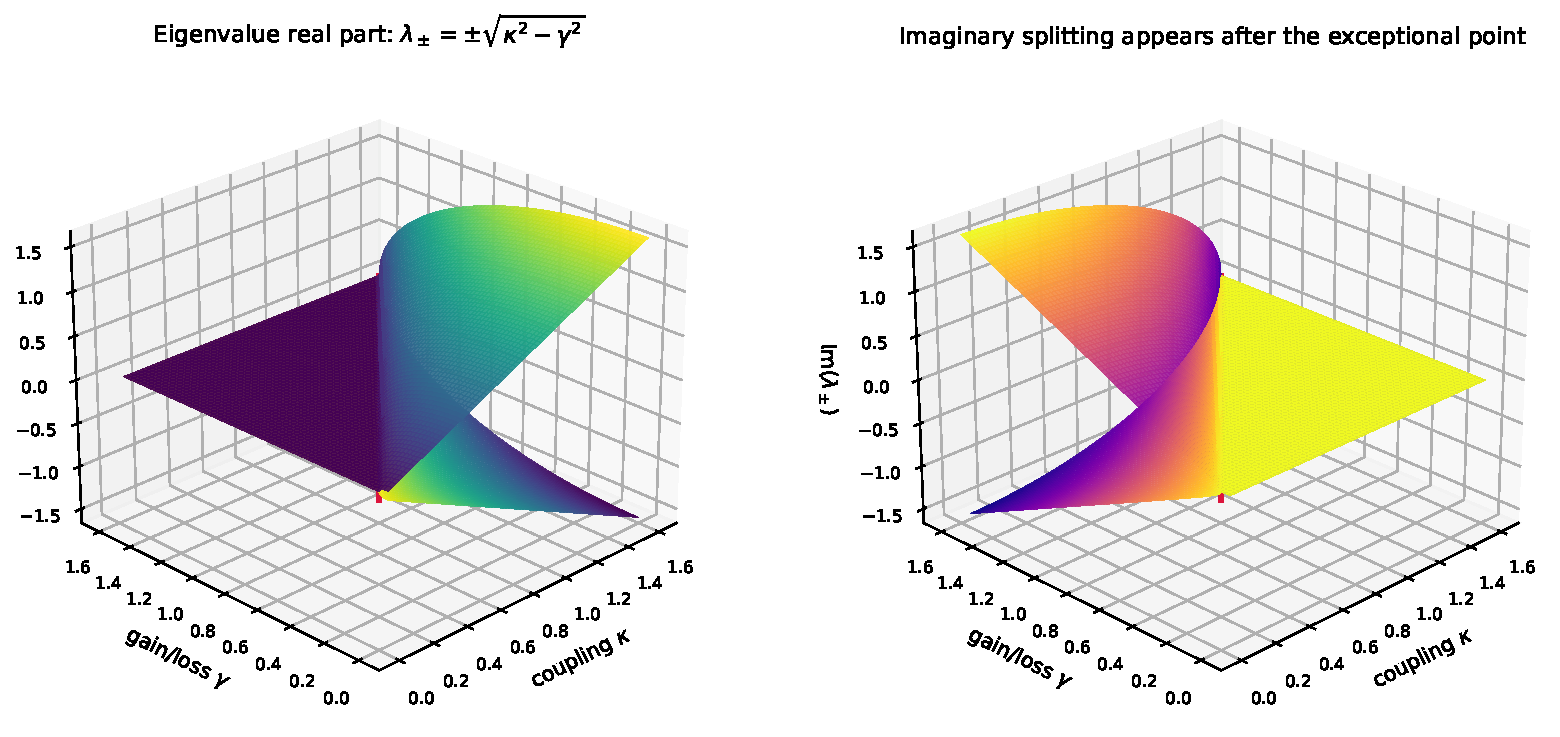
\includegraphics[width=0.98\textwidth]{fig_f8_ep_eigenvalues.pdf}
 \caption{Eigenvalue surfaces of the two-mode exceptional-point model
 $H=\begin{psmallmatrix} i\gamma & \kappa \\ \kappa & -i\gamma
 \end{psmallmatrix}$. The eigenvalues
 $\lambda_{\pm}=\pm\sqrt{\kappa^2-\gamma^2}$ are real split for
 $\gamma<\kappa$ and imaginary split for $\gamma>\kappa$; the red line
 marks the exceptional set $\gamma=\kappa$. This surface makes the
 square-root topology visible before any topological language is
 introduced.}
 \label{fig:ep-eigenvalue-surfaces}
\end{figure}



\subsection{Square-root topology}
\label{ssec:sqrt-topology}

Near the EP, the eigenvalues behave as
\begin{equation}
 \omtil_\pm \approx \omega_{\mathrm{EP}}
 \pm \sqrt{\alpha\,\Delta p},
 \label{eq:sqrt-response}
\end{equation}
where $\Delta p$ is the distance from the EP in parameter space and
$\alpha$ is a constant. This \emph{square-root} dependence---in contrast
to the linear splitting at a diabolic point---is the hallmark of an EP.
It means that the sensitivity of the eigenvalues to perturbations
diverges as $\Delta p \to 0$: $\dd\omtil/\dd p \propto 1/\sqrt{\Delta p}$.

The square-root topology has a concrete geometric interpretation: the
eigenvalue surface $\omtil(\delta)$ is a double-sheeted Riemann surface,
and the EP is the branch point connecting the two sheets. Any path in
parameter space that encircles the EP must cross from one sheet to the
other---the eigenvalue labels are exchanged after one circuit
(Section~\ref{sec:encircling}).

\subsection{Eigenvector coalescence}
\label{ssec:eigenvector-coalescence}

At the EP, the two eigenvectors of~\eqref{eq:ep-H} collapse onto a single
vector. Away from the EP, write the normalized right eigenvectors as
\begin{equation}
 |\psi_+\rangle =
 \begin{pmatrix} \cos\theta \\ \sin\theta \end{pmatrix},
 \qquad
 |\psi_-\rangle =
 \begin{pmatrix} -\sin\theta \\ \cos\theta \end{pmatrix},
 \label{eq:ep-evecs}
\end{equation}
where $\theta$ depends on $\delta/\kappa$. As the EP is approached
($\delta \to i\kappa$), $\theta \to \pi/4 + i\infty$, and both
eigenvectors approach the same direction
$|\psi_{\mathrm{EP}}\rangle \propto (1, i)^\transpose$. The overlap
$\langle\psi_+|\psi_-\rangle \to 1$: the modes become parallel.

\begin{figure}[t]
 \centering
 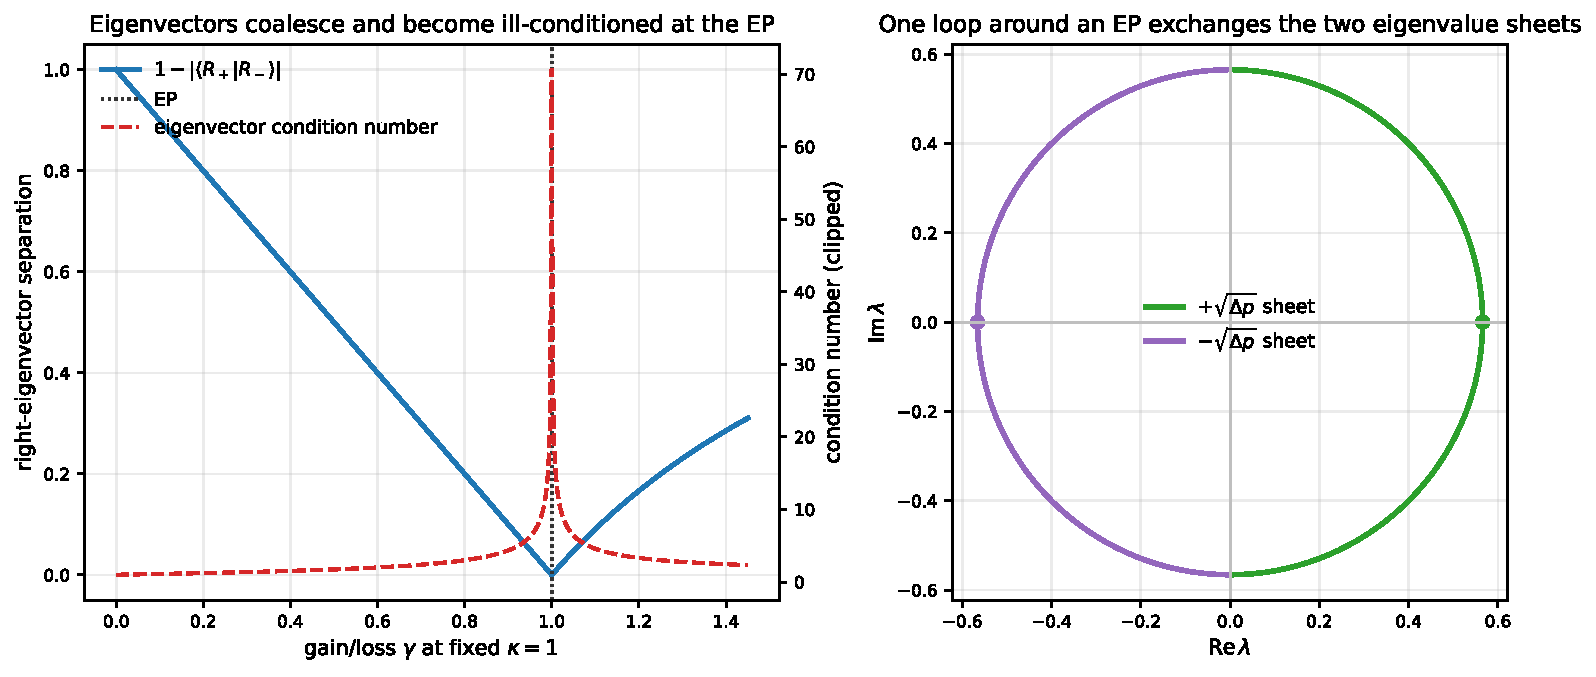
\includegraphics[width=0.95\textwidth]{fig_f8_ep_vectors.pdf}
 \caption{Eigenvector coalescence and branch-sheet exchange near a
 second-order exceptional point. Left: as $\gamma$ approaches
 $\kappa=1$, the two right eigenvectors become parallel and the
 eigenvector matrix becomes ill conditioned. Right: a closed loop
 around the branch point exchanges the two sheets of
 $\sqrt{\Delta p}$, so one circuit does not return an eigenvalue to
 itself.}
 \label{fig:ep-eigenvector-coalescence}
\end{figure}


%% ================================================================
\section{Jordan form and the generalized eigenvector}
\label{sec:jordan}

At the EP, the matrix $H$ cannot be diagonalized. Instead, it is brought
to Jordan normal form by a \emph{generalized eigenvector}
$|\chi\rangle$ satisfying
\begin{equation}
 (H - \omega_{\mathrm{EP}})\,|\chi\rangle = |\psi_{\mathrm{EP}}\rangle,
 \label{eq:jordan-chain}
\end{equation}
so that in the basis $\{|\psi_{\mathrm{EP}}\rangle, |\chi\rangle\}$,
\begin{equation}
 H = \omega_{\mathrm{EP}}\,\mathbf{I}
 + \begin{pmatrix} 0 & 1 \\ 0 & 0 \end{pmatrix}.
 \label{eq:jordan-block}
\end{equation}

\subsection{Dynamical consequences}
\label{ssec:jordan-dynamics}

The Jordan block has physical consequences: the time evolution of a
state initialized along $|\chi\rangle$ is
\begin{equation}
 e^{-iHt}\,|\chi\rangle
 = e^{-i\omega_{\mathrm{EP}}t}
 \bigl(|\chi\rangle - it\,|\psi_{\mathrm{EP}}\rangle\bigr),
 \label{eq:jordan-evolution}
\end{equation}
which grows \emph{linearly in time} before decaying exponentially. This
anomalous algebraic growth is the dynamical signature of the EP and
leads to enhanced transient responses.

More generally, for an EP$_n$ with Jordan block of size $n$, the time
evolution of the highest generalized eigenvector involves polynomial
growth $\propto t^{n-1}$ before exponential decay sets in. The
transient can dominate the dynamics for times $t \lesssim 1/\Delta\gamma$,
where $\Delta\gamma$ is the linewidth broadening near the EP~\cite{anderson2022clarification,smith2020beyond,smith2022beyond}.

\subsection{Pseudospectrum interpretation}
\label{ssec:jordan-pseudospectrum}

The defective nature of the matrix at an EP is intimately connected
to its pseudospectral properties
(Appendix~\ref{app:nonnormal}). Near an EP$_2$, the
$\epsilon$-pseudospectrum $\sigma_\epsilon(H)$ (the set of $z$ for which
$\|(zI-H)^{-1}\| \ge 1/\epsilon$) expands as
\begin{equation}
 \sigma_\epsilon(H) \supset
 \{z : |z - \omega_{\mathrm{EP}}| \le C\sqrt{\epsilon}\},
 \label{eq:pseudospectrum-ep}
\end{equation}
where $C$ depends on the Jordan-chain structure and normalization. The
$\sqrt{\epsilon}$ scaling of the pseudospectral radius---compared to
$\epsilon$ for a diagonalizable matrix---quantifies the extreme
sensitivity of the spectrum at an EP.


%% ================================================================
\section{Encircling an exceptional point}
\label{sec:encircling}

One of the most striking features of an EP is its topological character:
if the system parameters are varied adiabatically along a closed loop
encircling the EP in parameter space, the two eigenvalues are
\emph{exchanged}:
\begin{equation}
 \omtil_+ \xrightarrow{\text{one loop}} \omtil_-
 \xrightarrow{\text{two loops}} \omtil_+.
 \label{eq:eigenvalue-exchange}
\end{equation}
This is a consequence of the square-root branch point: the eigenvalue
surface $\omtil(\delta)$ is a double-valued Riemann surface, and the EP
is the branch point connecting its two sheets.

The eigenvectors also transform nontrivially under encircling. After one
loop, an eigenvector acquires a geometric (Berry-like) phase \emph{and}
exchanges identity with the other eigenvector:
\begin{equation}
 |\psi_+\rangle \xrightarrow{\text{one loop}} e^{i\phi}\,|\psi_-\rangle.
 \label{eq:evec-exchange}
\end{equation}
After \emph{two} loops, the original eigenvector is recovered up to a
geometric phase. This monodromy is unique to non-Hermitian systems and
has no analogue at diabolic points.

\subsection{Dynamic encircling}
\label{ssec:dynamic-encircling}

Static (adiabatic) encircling faces a practical limitation: near the EP,
the gap between eigenvalues shrinks to zero, and the adiabatic condition
$\dot{p}/\Delta\omega \ll 1$ cannot be maintained. Non-adiabatic
transitions can prevent the eigenvalue exchange.

\emph{Dynamic encircling}---varying parameters at a finite rate along a
loop that passes through or near the EP---reveals richer physics. The
system can exhibit chiral behavior: the final state depends on the
\emph{direction} of encircling (clockwise vs.\ counterclockwise). This
chirality has been demonstrated experimentally in waveguide systems and
provides a mechanism for topological mode switching and asymmetric
transmission.


%% ================================================================
\section{The Petermann factor at exceptional points}
\label{sec:petermann-ep}

The Petermann factor (Section~\ref{sec:petermann}) quantifies the
linewidth enhancement due to mode non-orthogonality. Near an EP$_2$,
the Petermann factor diverges as
\begin{equation}
 K \approx \frac{1}{|\langle L_+|R_+\rangle|^2}
 \propto \frac{1}{|\Delta p|},
 \label{eq:petermann-ep}
\end{equation}
where $\langle L_+|$ and $|R_+\rangle$ are the left and right
eigenvectors and $\Delta p$ is the distance from the EP in parameter
space. At the EP itself, $\langle L|R\rangle = 0$ and $K$ diverges.

\subsection{Physical consequences}
\label{ssec:petermann-physics}

The divergence of the Petermann factor has two important consequences:
\begin{enumerate}
 \item \textbf{Linewidth broadening:} the quantum-limited linewidth of
 a laser operating near an EP is broadened by a factor controlled by the
 mode non-orthogonality, conventionally represented by $K$ in the
 single-mode Schawlow--Townes limit:
 $\Delta\omega_{\mathrm{laser}} = K\,\Delta\omega_{\mathrm{ST}}$,
 where $\Delta\omega_{\mathrm{ST}}$ is the Schawlow--Townes
 linewidth of an orthogonal mode with the same output power and decay
 rate. Near the EP, this broadening counteracts the improved frequency
 splitting.
 \item \textbf{Noise amplification:} the quantum noise in any
 measurement performed on the system is amplified by the Petermann
 factor. For a homodyne or heterodyne detection scheme, the signal
 scales as $\sqrt{\epsilon}$ (the EP splitting) but the noise scales
 as $\sqrt{K} \propto 1/|\Delta p|^{1/2}$, and the signal-to-noise
 ratio can remain constant or even decrease.
\end{enumerate}

\subsection{Phase rigidity}
\label{ssec:phase-rigidity}

A complementary measure of non-Hermiticity is the \emph{phase rigidity}
\begin{equation}
 r_n = \frac{\langle L_n|R_n\rangle}{\langle R_n|R_n\rangle},
 \label{eq:phase-rigidity}
\end{equation}
after choosing a consistent normalization of the left and right
eigenvectors. In complex-symmetric reciprocal models this reduces to
the familiar unconjugated self-overlap divided by the usual norm. It
satisfies $|r_n| = 1$ for Hermitian systems (orthogonal modes) and
$|r_n| \to 0$ at an EP. With the same normalization convention, the
Petermann factor and phase rigidity are related by
$K_n = 1/|r_n|^2$, providing two complementary views of the same
non-Hermitian effect.


%% ================================================================
\section{Exceptional points in photonics}
\label{sec:ep-photonics}

\subsection{Coupled microring resonators}
\label{ssec:ep-microrings}

The most widely studied photonic EP platform consists of two evanescently
coupled microring resonators, one with gain and one with loss. The
effective Hamiltonian is exactly~\eqref{eq:ep-H} with $\delta = i\gamma$
(the gain--loss contrast) and $\kappa$ the evanescent coupling. The EP
occurs at $\gamma = \kappa$, and the transition from the $\PT$-symmetric
phase ($\gamma < \kappa$, real eigenvalue splitting) to the broken phase
($\gamma > \kappa$, complex splitting) is directly observable in the
transmission spectrum.

\subsection{Example: coupled microdisks}
\label{ssec:ep-worked-example}

Consider two whispering-gallery-mode microdisks at wavelength
$\lambda = 1550\;\mathrm{nm}$, each with intrinsic quality factor
$Q_0 = 10^6$ and resonance frequency
$\omega_0 = 2\pi c/\lambda \approx 1.216 \times 10^{15}\;\mathrm{rad/s}$.
The intrinsic decay rate is
$\gamma_0 = \omega_0/(2Q_0) \approx 6.08 \times 10^{8}\;\mathrm{rad/s}$.

One disk is pumped to provide gain, reducing its effective loss to
$\gamma_{\mathrm{gain}} = \gamma_0 - g$, while the other remains passive
with $\gamma_{\mathrm{loss}} = \gamma_0$. The gain--loss contrast is
$\gamma = (\gamma_{\mathrm{loss}} - \gamma_{\mathrm{gain}})/2 = g/2$.
The evanescent coupling rate between the disks is
$\kappa = 5 \times 10^9\;\mathrm{rad/s}$ (set by the inter-disk gap).

The EP condition $\gamma = \kappa$ requires $g = 2\kappa = 10^{10}\;\mathrm{rad/s}$,
corresponding to a material gain coefficient
$g_{\mathrm{mat}} = 2g n_g/c \approx 1\;\mathrm{cm^{-1}}$
(for group index $n_g \approx 1.5$). At the EP:
\begin{itemize}
 \item The two eigenfrequencies coalesce at $\omega_{\mathrm{EP}} = \omega_0 - i\gamma_0$.
 \item The eigenvectors collapse to
 $|\psi_{\mathrm{EP}}\rangle \propto (1, i)^\transpose$:
 a circularly phased superposition.
 \item The Petermann factor diverges.
 \item A perturbation $\delta\omega_0 = 10^6\;\mathrm{rad/s}$ (from a
 nanoparticle binding event) produces a splitting
 $\Delta\omega \approx \sqrt{2\kappa\,\delta\omega_0} \approx
 10^8\;\mathrm{rad/s}$---a $100\times$ enhancement over the
 diabolic-point splitting $\Delta\omega_{\mathrm{DP}} = \delta\omega_0$.
\end{itemize}
This example shows both the promise and the caveat of EP sensing: the
splitting is enhanced, but the linewidth broadening must be assessed
independently.

\paragraph{Geometric design considerations.}
For InP-based microdisks ($n_{\mathrm{eff}} \approx 2.6$,
radius $R = 15\;\mu$m, thickness $h = 220\;$nm), the whispering-gallery
modes have azimuthal order $m \approx 2\pi R n_{\mathrm{eff}}/\lambda
\approx 158$ near $\lambda = 1550\;$nm. The evanescent coupling rate
between two identical disks separated by a gap $d$ decays as
$\kappa \propto e^{-d/\ell}$, where the decay length
$\ell \approx \lambda/(2\pi\sqrt{n_{\mathrm{eff}}^2 - 1}) \approx
100\;$nm. For the coupling $\kappa = 5 \times 10^9\;$rad/s used above,
the required gap is $d \approx \ell\,\ln(\kappa_0/\kappa) \approx
300\;$nm, well within electron-beam lithography precision. The EP is
therefore accessible with standard nanofabrication.

The challenge lies in controlling the gain: the required material gain
$g_{\mathrm{mat}} \approx 1\;$cm$^{-1}$ must be matched to the
coupling rate within a tolerance
$\delta g/g \lesssim \gamma_0/\kappa \approx 0.12$ for the EP to be
resolvable above the natural linewidth. This $12\%$ tolerance is
achievable with careful pump calibration, but drift and thermal effects
can shift the system away from the EP during measurement.

\subsection{Waveguide systems}
\label{ssec:ep-waveguides}

Two coupled waveguides with different loss rates exhibit an EP as a
function of the inter-waveguide spacing (which controls $\kappa$) and
the loss contrast. The EP manifests as a transition from oscillatory
power exchange between the waveguides to unidirectional power transfer
toward the lossier guide.

\subsection{Single-resonator exceptional points}
\label{ssec:ep-single}

A single resonator can exhibit EPs when two of its QNMs are brought to
coalescence by tuning a geometric or material parameter. This does not
require gain or $\PT$ symmetry: two modes of a purely passive cavity can
coalesce at an EP if their radiation loss rates are appropriately matched.
The EP condition is then a statement about the radiation Q factors and
the inter-modal coupling mediated by the cavity shape.


%% ================================================================
\section{Sensing at exceptional points}
\label{sec:ep-sensing}

\subsection{Enhanced responsivity}
\label{ssec:ep-responsivity}

The square-root response~\eqref{eq:sqrt-response} near an EP has motivated
proposals for enhanced sensing. A small perturbation $\epsilon$ applied
to a system operating at an EP produces an eigenvalue splitting
\begin{equation}
 \Delta\omtil \propto \epsilon^{1/n},
 \label{eq:ep-sensing}
\end{equation}
where $n$ is the EP order. For an EP$_2$, the splitting is
$\propto \sqrt{\epsilon}$, which is much larger than the linear splitting
$\Delta\omega \propto \epsilon$ of a conventional (diabolic) degeneracy
for small $\epsilon$. This enhanced spectral \emph{responsivity} has been
demonstrated experimentally in optical and microwave resonators.

\subsection{The noise problem}
\label{ssec:ep-noise}

However, responsivity is not the same as sensitivity. The practical
utility of EP sensing depends on the \emph{signal-to-noise ratio} (SNR),
which involves both the signal (the frequency splitting) and the noise
(the linewidth and measurement uncertainty).

Zhang et al.\ developed a quantum noise theory for EP
sensors~\cite{zhang2018quantum} using the quantum Langevin equations and
input--output formalism. Their key finding is that the quantum noise in
the output signal diverges at the EP at the same rate as the responsivity
enhancement:
\begin{equation}
 \text{SNR}_{\mathrm{EP}} \le \text{SNR}_{\mathrm{DP}}
 \qquad\text{(for linear systems)},
 \label{eq:snr-bound}
\end{equation}
where the subscripts EP and DP refer to exceptional-point and
diabolic-point sensors, respectively. The enhanced splitting is exactly
canceled by the enhanced noise, and the fundamental sensitivity limit
(the quantum Cram\'er--Rao bound) is not improved.

\paragraph{Quantum Fisher information analysis.}
The fundamental precision limit for estimating a parameter $\epsilon$
is set by the quantum Cram\'er--Rao bound
$\delta\epsilon \ge 1/\sqrt{N\,\mathcal{F}_Q}$, where $N$ is the
number of measurements and $\mathcal{F}_Q$ is the quantum Fisher
information (QFI). For a two-mode bosonic system near an EP$_2$,
Zhang et al.\ showed that the QFI scales as
\begin{equation}
 \mathcal{F}_Q \propto \frac{1}{\theta^4}
 \quad\text{where}\quad \theta = \sqrt{|\gamma - \kappa|}
 \label{eq:qfi-ep}
\end{equation}
measures the distance from the EP~\cite{zhang2018quantum}. This
$\theta^{-4}$ divergence arises from the covariance-matrix
amplification: the output noise variance diverges as $\theta^{-4}$
through the non-orthogonality of the modes, exactly canceling the
$\theta^{-2}$ responsivity enhancement from the square-root
splitting. For the microdisk example above with
$\theta = 0.1\kappa$, the QFI is enhanced by a factor of $10^4$
relative to $\theta = \kappa$, but the noise variance is also
enhanced by $10^4$, leaving the SNR unchanged.

Wang et al.\ confirmed this prediction experimentally in a Brillouin
ring laser gyroscope~\cite{wang2020petermann}: the enhanced transduction
of rotation signals near the EP was precisely canceled by
Petermann-factor linewidth broadening, leaving the fundamental angular
velocity sensitivity unchanged.

\subsection{Can nonlinearity help?}
\label{ssec:ep-nonlinear-sensing}

One hope for circumventing the noise--sensitivity cancellation is
nonlinearity. Above the lasing threshold, gain saturation creates a
nonlinear operating point where the instantaneous Hamiltonian may avoid
the EP. Zheng and Chong showed, however, that noise fluctuations shift
the nonlinear operating point away from the EP, effectively reducing the
EP order and preventing the system from exploiting the full $\epsilon^{1/n}$
responsivity~\cite{zheng2024noise}. Moreover, the Bogoliubov--de~Gennes
Hamiltonian governing small fluctuations around the nonlinear steady state
has its own EP structure, which can produce noise divergences stronger
than the simple Petermann estimate from the linear system.

\begin{takeaway}[EP sensing: a balanced view]
The frequency splitting at an EP scales as $\epsilon^{1/n}$, increasing
the local responsivity. But the fundamental sensitivity
(signal-to-noise ratio) may not improve because the Petermann factor and
quantum noise diverge at the same rate. Practical EP sensing may still
offer advantages through classical signal processing, readout
engineering, or operation in regimes where noise sources differ from the
fundamental quantum limit---but these advantages must be demonstrated
case by case, not assumed from the $\epsilon^{1/n}$ scaling alone.
\end{takeaway}


%% ================================================================
\section{Higher-order exceptional points}
\label{sec:higher-ep}

An EP of order $n$ (EP$_n$) occurs when $n$ eigenvalues and eigenvectors
coalesce simultaneously. The eigenvalue splitting near an EP$_n$ scales as
\begin{equation}
 \Delta\omtil \propto \epsilon^{1/n},
 \label{eq:epn-response}
\end{equation}
offering even greater responsivity enhancement for small perturbations.

\paragraph{Concrete example: EP$_3$ in three coupled cavities.}
Consider three identical microring resonators in a linear chain, each
with resonance $\omega_0$ and decay rate $\gamma_0$, with nearest-neighbour
coupling $\kappa$ and gain--loss distribution
$(+i\gamma,\; 0,\; -i\gamma)$. The effective Hamiltonian is
\begin{equation}
 H_{\mathrm{EP}_3} = \begin{pmatrix}
 \omega_0 + i\gamma & \kappa & 0 \\
 \kappa & \omega_0 & \kappa \\
 0 & \kappa & \omega_0 - i\gamma
 \end{pmatrix}.
 \label{eq:ep3-hamiltonian}
\end{equation}
For this symmetric trimer the EP$_3$ occurs when the two nonzero
eigenvalues collapse onto the central eigenvalue. Shift to the
co-rotating frame $E \equiv \omtil - \omega_0$ and write the
characteristic polynomial of~\eqref{eq:ep3-hamiltonian}:
\begin{equation}
 \det(H_{\mathrm{EP}_3} - \omtil\,\mathbf{I})
 = -E\left[E^2 - (2\kappa^2-\gamma^2)\right] = 0.
 \label{eq:ep3-charpoly}
\end{equation}
Thus the spectrum is $E_0=0$ and
$E_\pm=\pm\sqrt{2\kappa^2-\gamma^2}$. At
$\gamma=\sqrt{2}\,\kappa$, all three eigenvalues coalesce at
$E_{\mathrm{EP}}=0$. The matrix is then defective: it has a single
eigenvector and is similar to a $3\times3$ Jordan block. This is the
third-order exceptional point. More general EP$_3$ realizations require
the expected four real tuning conditions, but the symmetry of this model
reduces the number of independent knobs.

Now introduce a small perturbation---for instance, a detuning
$\epsilon$ applied to the middle cavity, so that
$H_{22} \to \omega_0 + \epsilon$. The characteristic polynomial
becomes
\begin{equation}
 -E^3 + \epsilon\,(E^2+\gamma^2) + \cdots = 0
 \qquad (\gamma=\sqrt{2}\,\kappa).
 \label{eq:ep3-perturbed}
\end{equation}
Near the coalescence point, write $E = E_{\mathrm{EP}} + \delta E$ and
expand to leading order in $\epsilon$. The triple-root structure means
that the unperturbed part contributes $-(\delta E)^3$ at lowest order,
while the perturbation contributes a constant term
$\gamma^2\epsilon$.
Balancing these:
\begin{equation}
 (\delta E)^3 \sim \gamma^2\,\epsilon
 \quad\Longrightarrow\quad
 \delta E_j \approx (\gamma^2\,\epsilon)^{1/3}\,e^{2\pi i j/3},
 \quad j = 0, 1, 2,
 \label{eq:ep3-cuberoot}
\end{equation}
up to a convention-dependent phase set by the sign of the perturbation.
The three eigenvalue branches are related by a
$2\pi/3$ phase rotation in the complex plane, forming a three-sheeted
Riemann surface. Encircling the EP$_3$ in parameter space cycles
through all three eigenvalues, requiring three full loops to return to
the starting sheet---in contrast to the two loops needed at an EP$_2$.

The cube-root scaling strongly affects sensing estimates.
A perturbation of magnitude $|\epsilon| = 10^{-9}$ (in units of
$\kappa$) produces a splitting
$|\delta E| \sim 10^{-3}\kappa$, compared to $10^{-9}\kappa$ at a
diabolic point and $10^{-4.5}\kappa$ at an EP$_2$. However, as
discussed in Section~\ref{sec:ep-sensing}, the Petermann factor
diverges as $K \sim |\epsilon|^{-2(n-1)/n}$ near an EP$_n$, so the
noise enhancement at an EP$_3$ scales as $|\epsilon|^{-4/3}$ in the
same perturbative normalization. This growth can erase the apparent
responsivity advantage. Whether a net SNR improvement survives depends
on the specific noise model and measurement protocol.

The Jordan block at the EP$_3$ is $3\times 3$, producing quadratic
transient growth $\propto t^2$ before exponential decay:
\begin{equation}
 e^{-iH_{\mathrm{EP}_3}\,t}
 = e^{-i E_{\mathrm{EP}}\,t}\left(
 \mathbf{I} - i\,N\,t - \tfrac{1}{2}N^2 t^2\right),
 \label{eq:ep3-time-evolution}
\end{equation}
where $N$ is the nilpotent part ($N^3 = 0$). This quadratic growth
is directly observable as a transient intensity amplification in a
pulsed excitation experiment.

Experimental demonstrations of EP$_3$ have used coupled fiber
loops~\cite{meng2023exceptional} and coupled microwave cavities with
carefully calibrated gain--loss profiles; in photonics, the primary
challenge is maintaining the $2(n-1) = 4$ parameter tuning conditions
simultaneously against fabrication disorder and thermal drift.

\subsection{Realization challenges}
\label{ssec:higher-ep-realization}

Realizing EP$_n$ with $n > 2$ requires tuning $2(n-1)$ real parameters
to coalescence, which becomes increasingly difficult. Experimental
demonstrations of EP$_3$ have been achieved in coupled-resonator systems
with engineered gain and loss profiles. The Jordan block at EP$_n$ is
$n\times n$, and the time evolution involves polynomial growth
$\propto t^{n-1}$ before exponential decay. Encircling an EP$_n$ in
parameter space exchanges eigenvalues cyclically, with a period of $n$
loops.

\begin{figure}[t]
 \centering
 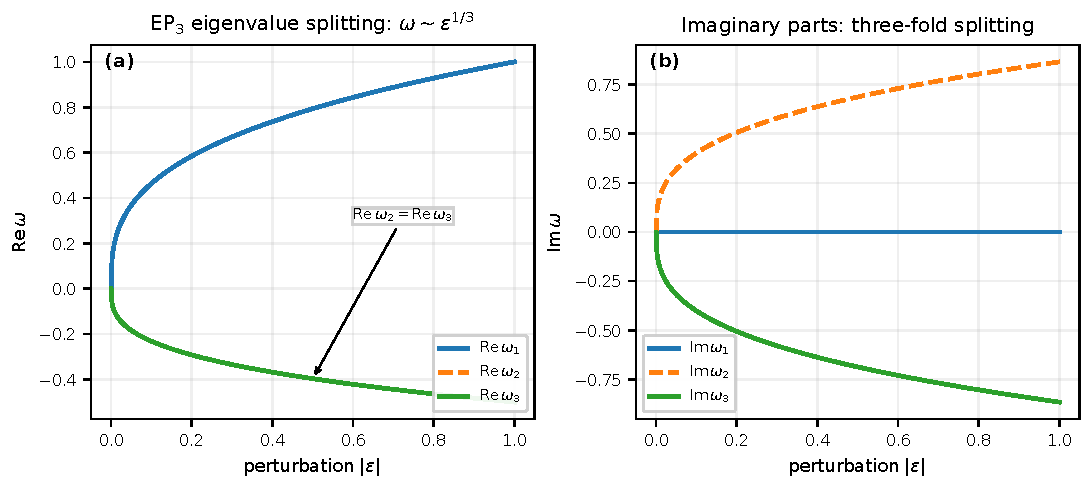
\includegraphics[width=0.95\linewidth]{fig_f8_ep3_splitting.pdf}
 \caption{Eigenvalue splitting near a third-order exceptional point
 (EP$_3$). A perturbation of magnitude $|\epsilon|$ lifts the
 three-fold degeneracy as $\omega_j \sim \epsilon^{1/3}\,
 e^{2\pi i j/3}$ ($j = 1,2,3$).
 (a)~Real parts: $\Re\omega_1 = |\epsilon|^{1/3}$ (blue,
 solid) rises above the EP, while
 $\Re\omega_2 = \Re\omega_3 = -\tfrac{1}{2}|\epsilon|^{1/3}$
 (orange dashed and green solid, exactly overlapping) descend
 together---a hallmark of the cube-root topology.
 (b)~Imaginary parts split into three distinct branches:
 $\Im\omega_1 = 0$ and
 $\Im\omega_{2,3} = \pm\tfrac{\sqrt{3}}{2}|\epsilon|^{1/3}$.}
 \label{fig:ep3-splitting}
\end{figure}

\subsection{Noise scaling at higher-order EPs}
\label{ssec:higher-ep-noise}

The noise cancellation described in Section~\ref{ssec:ep-noise} becomes
\emph{more} severe at higher-order EPs. If a perturbation $\epsilon$
splits an EP$_n$ as $\Delta\omega\sim \epsilon^{1/n}$, the associated
eigenvectors become increasingly self-orthogonal and the Petermann
factor typically scales as
$K\sim |\epsilon|^{-2(n-1)/n}$ in the same local perturbative model.
Thus the larger responsivity is accompanied by stronger excess noise and
linewidth broadening. The precise SNR scaling depends on the readout and
noise model, but higher order alone is not a route to guaranteed
fundamental sensitivity enhancement.


%% ================================================================
\section{Exceptional points and topology}
\label{sec:ep-topology}

Exceptional points are topological objects in parameter space. The
eigenvalue exchange under encircling (Section~\ref{sec:encircling})
defines a topological invariant: the \emph{discriminant number}, which
counts the number of EPs enclosed by a loop. This invariant is robust
against smooth deformations of the loop that do not cross an EP.

In the band structure of periodic non-Hermitian systems, EPs appear as
\emph{exceptional lines} or \emph{exceptional surfaces} in the
Brillouin zone, where two complex bands touch. These structures carry
topological charges and can be classified by the homotopy groups of the
relevant classifying spaces.

\subsection{EP charges and conservation}
\label{ssec:ep-charges}

Each EP$_2$ in a 2D parameter space carries a topological charge
$\nu = \pm 1/2$, defined as the winding of the eigenvalue-branch phase
around the EP. The total charge in any region of parameter space is
conserved: EPs can be created or annihilated only in pairs with opposite
charges. This conservation law constrains the possible arrangements of
EPs in the Brillouin zone and explains why isolated EPs are robust
against perturbations that do not create new degeneracies.

\subsection{Connection to band topology}
\label{ssec:ep-band-topology}

The connection between EPs and band topology is developed further in
Chapter~\ref{ch:complex-bands}, where EPs appear as singular points in
the complex band structure. The $\pi$ Berry phase encircling an EP in
momentum space (Section~\ref{ssec:berry-ep}) provides a direct link
between the EP charge and the topological invariants of the non-Hermitian
band structure.

\begin{takeaway}[Exceptional points as organizing principle]
Exceptional points are the fundamental singularities of non-Hermitian
spectral theory. They organize the parameter space of photonic systems
into regions of qualitatively different behavior: oscillatory versus
overdamped dynamics, symmetric versus broken $\PT$ phases, and distinct
topological sectors. Their square-root topology, Jordan-block dynamics,
Petermann-factor divergence, and connection to band topology make them
central to non-Hermitian photonics at every scale, from nanophotonic
cavities to macroscopic laser systems.
\end{takeaway}

\chapter{$\PT$-Symmetric Optics}
\label{ch:pt-symmetric}

\begin{chapterlead}
Among all non-Hermitian photonic systems, those with parity--time ($\PT$)
symmetry occupy a special place. A $\PT$-symmetric structure has a
refractive-index profile that satisfies $n(\rr) = n^*(-\rr)$: the real
part is symmetric and the imaginary part is antisymmetric under spatial
inversion. Gain and loss are balanced, and the system can exhibit a
$\PT$ phase transition~\cite{elganainy2007theory}---from a regime with entirely real
eigenfrequencies to one with complex conjugate pairs---controlled by a
single parameter. The $\PT$-symmetry condition is derived from the
Helmholtz equation, followed by the transfer-matrix theory for $\PT$
Bragg gratings and the associated phenomena: spontaneous
$\PT$-symmetry breaking, unidirectional invisibility, and the connection
to exceptional points.
\end{chapterlead}


%% ================================================================
\section{The $\PT$-symmetry condition}
\label{sec:pt-condition}

\subsection{Parity and time reversal in Maxwell's equations}
\label{ssec:pt-maxwell}

The parity operator $\mathcal{P}$ acts by spatial inversion:
$\mathcal{P}\EE(\rr) = -\EE(-\rr)$, $\mathcal{P}\HH(\rr) = \HH(-\rr)$
(the signs follow from the vector and pseudovector character of $\EE$ and
$\HH$). The time-reversal operator $\mathcal{T}$ acts by complex
conjugation on the frequency-domain fields: $\mathcal{T}\EE(\rr) =
\EE^*(\rr)$, which reverses the sign of $\omega$ and exchanges incoming
and outgoing waves.

A system described by a spatially varying permittivity $\epsr(\rr)$ is
$\PT$-symmetric if the combined operation $\PT$ leaves the Helmholtz
equation invariant. For the scalar Helmholtz equation
\begin{equation}
 -\nabla^2\psi(\rr) = \frac{\omega^2}{c^2}\,n^2(\rr)\,\psi(\rr),
 \label{eq:helmholtz-scalar}
\end{equation}
the $\PT$ transformation maps $\psi(\rr) \to \psi^*(-\rr)$ and requires
\begin{equation}
 \boxed{n^2(\rr) = [n^2(-\rr)]^*,}
 \label{eq:pt-n-condition}
\end{equation}
or equivalently for the permittivity:
$\epsr(\rr) = \epsr^*(-\rr)$. This means
\begin{equation}
 \epsr'(\rr) = \epsr'(-\rr), \qquad
 \epsr''(\rr) = -\epsr''(-\rr):
 \label{eq:pt-eps-parts}
\end{equation}
the real part of the permittivity is spatially even and the imaginary part
is spatially odd. Regions of gain and loss are arranged as mirror images.

\subsection{$\PT$ symmetry does not mean Hermiticity}
\label{ssec:pt-not-hermitian}

A $\PT$-symmetric system has complex $\epsr(\rr)$; it is not Hermitian.
However, the balance of gain and loss allows the eigenfrequencies to be
real over a range of parameters---the \emph{$\PT$-symmetric phase}. The
eigenfrequencies become complex only when the gain--loss contrast exceeds
a critical threshold: the $\PT$-breaking transition, which occurs at an
exceptional point (Chapter~\ref{ch:exceptional-points}).

It is worth stating exactly what $\PT$ symmetry does and does not
guarantee:
\begin{itemize}
 \item It \emph{does} guarantee that eigenvalues come in conjugate
 pairs or are real: if $\omtil$ is an eigenvalue, so is $\omtil^*$.
 \item It \emph{does not} guarantee that all eigenvalues are real.
 The transition from real to complex eigenvalues is spontaneous
 symmetry breaking: the eigenstates cease to be simultaneous
 eigenstates of $\PT$.
 \item It \emph{does not} guarantee stability. Even in the
 $\PT$-symmetric phase, the non-normality of the Hamiltonian can
 produce large transient growth
 (Section~\ref{sec:matrix-exp}).
\end{itemize}

\subsection{$\PT$ symmetry from the energy inner product}
\label{ssec:pt-energy}

The relation between $\PT$ symmetry and the energy inner product of
Chapter~\ref{ch:energy-inner} can be made precise. The Maxwell
curl--curl operator $\hat{\Theta}$ is self-adjoint with respect to
the $\epsr$-weighted inner product when $\epsr$ is real. When
$\epsr$ is complex but satisfies $\epsr(\rr) = \epsr^*(-\rr)$, the
operator is no longer self-adjoint in the standard inner product, but
it commutes with the antilinear operator $\PT$:
\begin{equation}
 [\hat{\Theta},\,\PT] = 0
 \qquad\text{when}\qquad
 \epsr(\rr) = \epsr^*(-\rr).
 \label{eq:theta-pt-commute}
\end{equation}
This commutation replaces self-adjointness as the organizing symmetry
of the spectrum. Bender and Boettcher first recognized this structure
in quantum mechanics; in photonics, it descends directly from the
Maxwell equations.


%% ================================================================
\section{$\PT$ phase transition in the two-mode model}
\label{sec:pt-two-mode}

The simplest $\PT$-symmetric system is a pair of coupled resonances with
equal and opposite gain/loss rates, described by the effective Hamiltonian
\begin{equation}
 H_{\PT} =
 \begin{pmatrix}
 \omega_0 + i\gamma & \kappa \\
 \kappa & \omega_0 - i\gamma
 \end{pmatrix},
 \label{eq:pt-hamiltonian}
\end{equation}
where $\gamma > 0$ is the gain/loss rate and $\kappa > 0$ is the real
coupling. The eigenvalues are
\begin{equation}
 \omtil_\pm = \omega_0 \pm \sqrt{\kappa^2 - \gamma^2}.
 \label{eq:pt-eigenvalues}
\end{equation}

\begin{figure}[t]
 \centering
 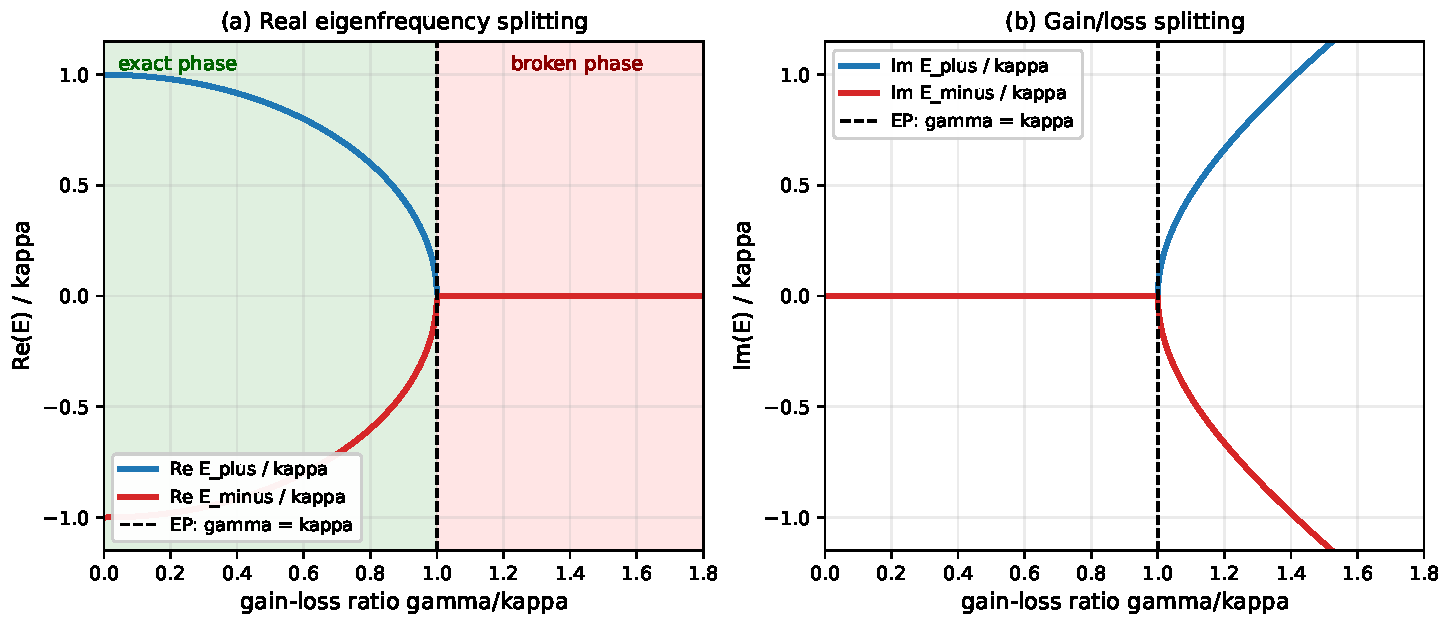
\includegraphics[width=0.85\linewidth]{figures/fig_f09_pt_phase_diagram.pdf}
 \caption{$\PT$ phase transition in the two-mode model.
 (a)~Real parts of the eigenvalues: in the exact $\PT$-symmetric
 phase ($\gamma < \kappa$, green shading) both eigenfrequencies are
 real and split; in the broken phase ($\gamma > \kappa$, red shading)
 they coalesce.
 (b)~Imaginary parts: zero throughout the exact phase, then
 bifurcating symmetrically in the broken phase. The exceptional point
 at $\gamma = \kappa$ (dashed line) marks the phase boundary where
 eigenvalues and eigenvectors simultaneously coalesce.}
 \label{fig:pt-phase-diagram}
\end{figure}

\paragraph{$\PT$-symmetric phase ($\gamma < \kappa$).}
The square root is real, and the eigenfrequencies $\omtil_\pm$ are both
real despite the non-Hermiticity of $H_{\PT}$. The modes are extended
over both resonators with equal gain and loss, so each mode experiences
zero net amplification.

\paragraph{$\PT$-broken phase ($\gamma > \kappa$).}
The square root becomes imaginary, and the eigenfrequencies form a complex
conjugate pair:
$\omtil_\pm = \omega_0 \pm i\sqrt{\gamma^2 - \kappa^2}$. One mode is
amplified, the other is attenuated. The gain--loss contrast has overcome
the coupling.

\paragraph{The exceptional point ($\gamma = \kappa$).}
At the transition, the eigenvalues coalesce at $\omega_0$ and the
eigenvectors merge. This is an EP$_2$ of exactly the type analyzed in
Section~\ref{sec:ep2}.

\subsection{Coupled-mode derivation from Maxwell fields}
\label{ssec:pt-cmt-maxwell}

The two-mode Hamiltonian~\eqref{eq:pt-hamiltonian} is not postulated
but derived from the Maxwell equations via the coupled-mode formalism of
Chapter~\ref{ch:maxwell-coupled-modes}. Consider two weakly coupled
cavities with identical real permittivity profiles but opposite imaginary
parts: cavity~A has $\varepsilon_A = \varepsilon_0 + i\kappa_I$ and cavity~B
has $\varepsilon_B = \varepsilon_0 - i\kappa_I$. The QNM framework of
Chapter~\ref{ch:qnm} gives each isolated cavity the same resonance
frequency $\omega_0$ but opposite imaginary corrections:
\begin{equation}
 \omtil_A = \omega_0 - i\gamma_{\mathrm{rad}} - i\gamma_{\mathrm{mat}},
 \qquad
 \omtil_B = \omega_0 - i\gamma_{\mathrm{rad}} + i\gamma_{\mathrm{mat}},
 \label{eq:pt-isolated-modes}
\end{equation}
where $\gamma_{\mathrm{rad}}$ is the (common) radiative decay rate and
$\gamma_{\mathrm{mat}} \propto \kappa_I$ is the material loss/gain rate
for the sign convention used here. Thus cavity~A is the lossy partner
and cavity~B is the gain partner for $\kappa_I>0$.
When the two cavities are brought into evanescent proximity, the overlap
integral of the reaction inner product
(Section~\ref{sec:reaction}) gives a coupling matrix element
$\kappa$ that is real and symmetric for reciprocal media. The
resulting $2\times 2$ effective Hamiltonian is exactly of the
form~\eqref{eq:pt-hamiltonian}, after subtracting the common offset
$\omega_0-i\gamma_{\mathrm{rad}}$ and identifying
$\gamma = \gamma_{\mathrm{mat}}$ up to the ordering of the two basis
states.

The Maxwell derivation shows explicitly that the $\PT$ condition for the
two-mode model---equal and opposite imaginary diagonal entries---is a
consequence of the $\PT$ condition for the permittivity, not an
independent postulate. It also reveals when the two-mode description
breaks down: when the coupling $\kappa$ is comparable to the mode
spacing, or when higher-order modes contribute significantly.


%% ================================================================
\section{Transfer-matrix theory for $\PT$ gratings}
\label{sec:pt-transfer}

\subsection{The 1D $\PT$-symmetric Bragg grating}
\label{ssec:pt-bragg}

Consider a one-dimensional periodic structure with refractive index
\begin{equation}
 n(x) = n_0 + \Delta n\cos(2\pi x/\Lambda)
 + i\Delta n_I\sin(2\pi x/\Lambda),
 \label{eq:pt-grating-n}
\end{equation}
where $n_0$ is the background index, $\Delta n$ is the real modulation
depth, $\Delta n_I$ is the imaginary modulation depth, and $\Lambda$ is
the period. This profile satisfies $n(x) = n^*(-x)$: it is
$\PT$-symmetric. When $\Delta n = 0$ and only the imaginary modulation
remains, the grating is purely gain--loss modulated.

\subsection{Transfer matrix for one period}
\label{ssec:pt-transfer-matrix}

Each period of the grating is a layered structure that can be described
by a $2\times 2$ transfer matrix $\Tmat$ relating the forward- and
backward-propagating wave amplitudes on the left to those on the right
(Appendix~\ref{app:transfer}). For a grating of $N$ periods, the total
transfer matrix is $\Tmat^N$.

The scattering matrix is obtained from $\Tmat$ by the standard conversion.
The reflection and transmission coefficients are~\cite{lin2011unidirectional}
\begin{equation}
 r_L = -\frac{T_{21}}{T_{22}}, \quad
 r_R = \frac{T_{12}}{T_{22}}, \quad
 t = \frac{1}{T_{22}},
 \label{eq:pt-transfer-to-scatter}
\end{equation}
where $T_{ij}$ are the elements of $\Tmat^N$.

\subsection{Example: a $\PT$ bilayer}
\label{ssec:pt-bilayer-example}

To make the transfer-matrix formalism concrete, consider the simplest
$\PT$ structure: a single unit cell with a loss slab
($n_1 = 3.0 + 0.05\,i$, thickness $d = 200\;\mathrm{nm}$) and a gain
slab ($n_2 = 3.0 - 0.05\,i$, same thickness). At wavelength
$\lambda = 1550\;\mathrm{nm}$, the propagation phase per slab is
$\phi = n k_0 d \approx 2.43 + 0.041\,i$ rad.

The single-slab propagation matrix is (Appendix~\ref{app:transfer})
\begin{equation}
 M_j = \begin{pmatrix} e^{in_j k_0 d} & 0 \\ 0 & e^{-in_j k_0 d} \end{pmatrix},
 \label{eq:pt-slab-matrix}
\end{equation}
and the interface matrix between slabs with indices $n_a$ and $n_b$ is
$I_{ab} = \tfrac{1}{2n_b}\bigl(\begin{smallmatrix} n_b+n_a & n_b-n_a
\\ n_b-n_a & n_b+n_a \end{smallmatrix}\bigr)$.
The unit-cell transfer matrix is
$\Tmat_{\mathrm{cell}} = I_{2,\mathrm{out}} \cdot M_2 \cdot I_{12}
\cdot M_1 \cdot I_{\mathrm{in},1}$.

For this example, the trace of $\Tmat_{\mathrm{cell}}$ is nearly real
and satisfies $|\tfrac{1}{2}\tr\Tmat_{\mathrm{cell}}| < 1$: the system is
in the $\PT$-symmetric phase. The left and right reflection
coefficients are
\begin{equation}
 |r_L| \approx 0.033, \qquad |r_R| \approx 0.034, \qquad
 |t| \approx 1.002,
 \label{eq:pt-bilayer-numbers}
\end{equation}
showing near-unit transmission with slightly asymmetric reflection.
The asymmetry grows with the number of unit cells $N$.

\begin{figure}[t]
 \centering
 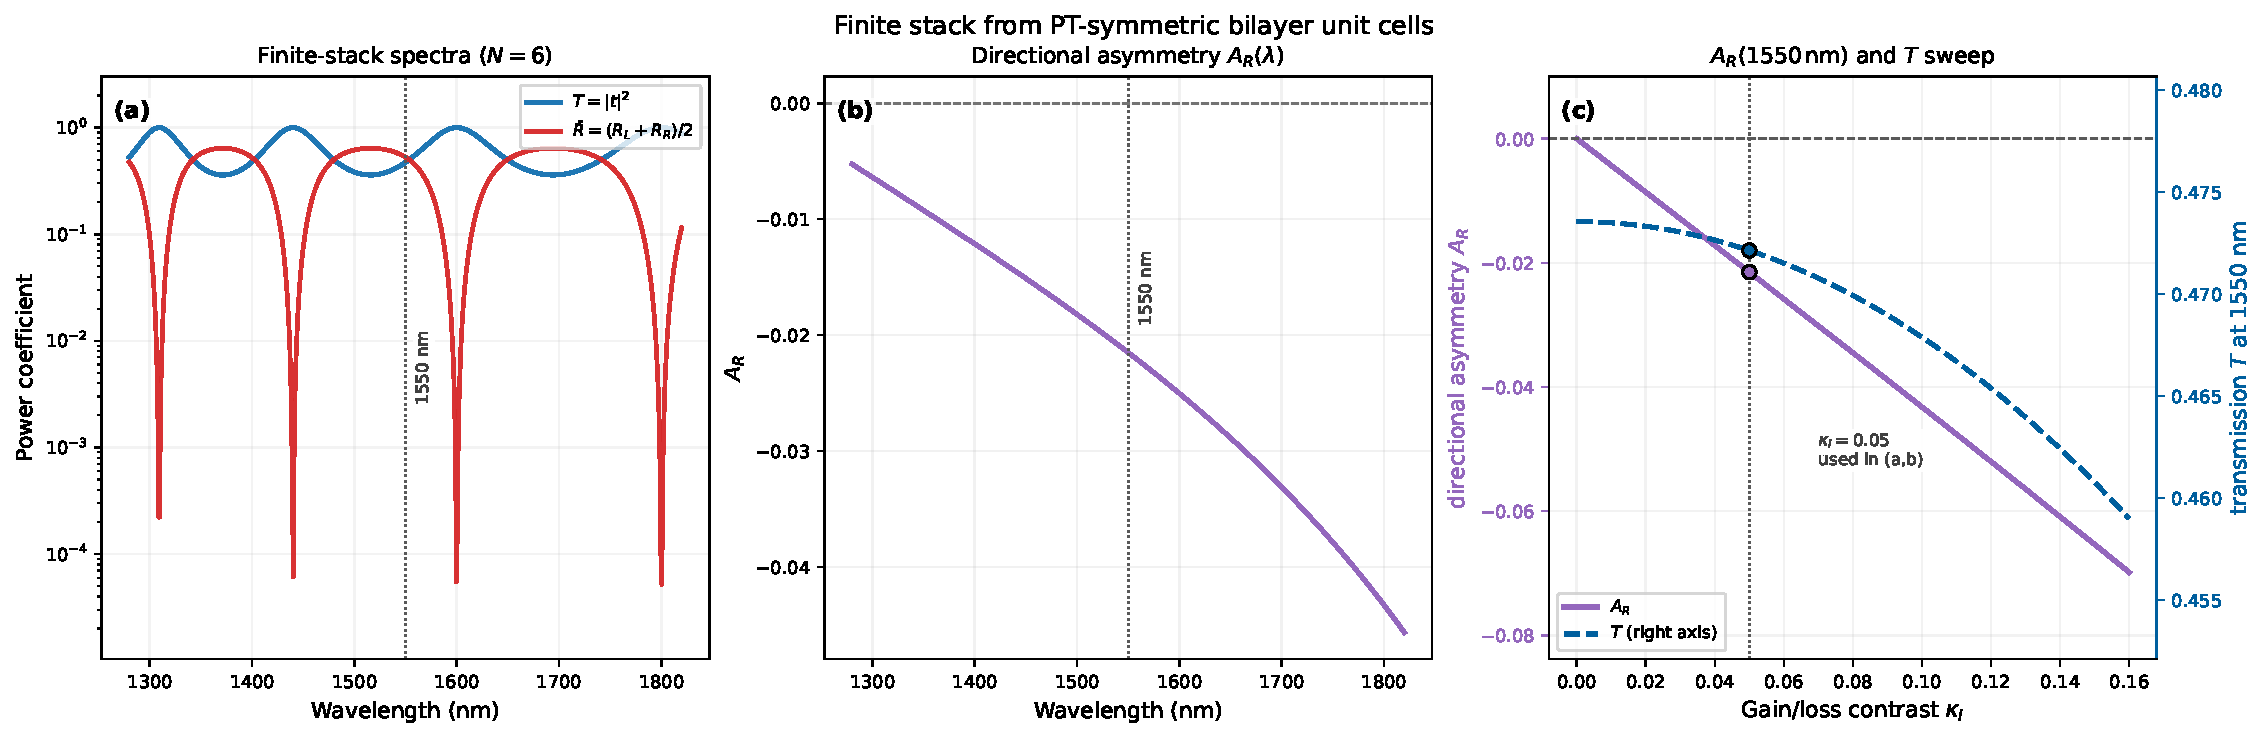
\includegraphics[width=0.98\textwidth]{fig_f9_pt_bilayer_spectra.pdf}
 \caption{Transfer-matrix spectra of a finite stack built from $\PT$-symmetric bilayer unit cells. The unit cell is the loss--gain pair used in this example, repeated $N=6$ times and embedded in air. Panel (a) shows the wavelength dependence of transmission $T=|t|^2$ and the mean reflectance $\bar R=(R_L+R_R)/2$; because the stack contains gain and loss, these are scattering intensities rather than a unitary energy partition. The small left--right difference is not visually useful on the logarithmic spectrum, so panel (b) plots the directional reflection asymmetry $A_R(\lambda)=(R_R-R_L)/(R_R+R_L)$ directly; negative $A_R$ means stronger reflection for left incidence. Panel (c) fixes $\lambda=1550\,\mathrm{nm}$ and varies the gain--loss index contrast $\kappa_I$, showing $A_R(1550\,\mathrm{nm})$ and the transmission $T$ as functions of gain/loss strength.}
 \label{fig:pt-bilayer-spectra}
\end{figure}

\subsection{Unidirectional invisibility}
\label{ssec:unidirectional}

Suitably designed $\PT$ Bragg gratings can exhibit
\emph{unidirectional invisibility}: at a scattering exceptional point or
anisotropic transmission resonance, the grating can be transparent from
one side ($r_L = 0$, $|t| = 1$) while remaining reflective from the other
side ($r_R \neq 0$)~\cite{lin2011unidirectional}. This is not a generic
consequence of every $\PT$-breaking point; it requires the grating
parameters and operating frequency to satisfy the corresponding
scattering condition.

The physical mechanism can be understood from the transfer-matrix
eigenvalue structure. At the EP, one eigenvalue has unit modulus
while the other is its inverse: $\lambda_+ = 1/\lambda_-^*$. The
corresponding eigenvectors correspond to forward- and backward-traveling
Bloch waves. For incidence from one side, the field couples
predominantly to the non-growing eigenstate and passes through with
unit transmission and zero reflection; for incidence from the other
side, the field excites the growing eigenstate, producing finite
reflection.

This asymmetry is not a violation of reciprocity---the transmission
coefficient is the same from both sides ($t_L = t_R$ for a reciprocal
medium)---but the reflection coefficients differ:
$|r_L| \neq |r_R|$. In a lossless reciprocal one-dimensional grating,
$|r_L| = |r_R|$ follows from the combination of reciprocity and flux
conservation. In the $\PT$-symmetric case, flux conservation is broken
and the two reflection magnitudes can differ even though the
transmission amplitude remains reciprocal.

\subsection{Spectral features near the Bragg condition}
\label{ssec:pt-bragg-spectrum}

The most dramatic $\PT$ effects occur near the Bragg condition
$\lambda = 2 n_0 \Lambda$, where the stop band of a conventional
(Hermitian) grating is located. In the $\PT$-symmetric grating:
\begin{itemize}
 \item Below the EP: the stop band splits into two narrower bands
 separated by a transmission peak at the Bragg wavelength.
 \item At the EP: the two bands merge, and the central peak becomes
 a unity-transmission point with divergent group delay---a critical
 slowing of light.
 \item Above the EP: the merged band becomes an amplification window
 for one scattering channel and an absorption window for the other.
\end{itemize}

These features have been observed experimentally in coupled-fiber
systems and semiconductor gratings, confirming the transfer-matrix
predictions quantitatively.

\begin{takeaway}[$\PT$ gratings break reflection symmetry, not reciprocity]
A $\PT$-symmetric Bragg grating is reciprocal ($t_L = t_R$) but not
unitary ($|r_L| \neq |r_R|$). The asymmetric reflection is a direct
consequence of balanced gain and loss, and it vanishes in the Hermitian
limit ($\Delta n_I \to 0$). This distinction between reciprocity and
unitarity echoes the general principle established in
Section~\ref{sec:reciprocity}.
\end{takeaway}


%% ================================================================
\section{$\PT$ symmetry of the scattering matrix}
\label{sec:pt-smatrix}

For a one-dimensional two-port $\PT$-symmetric structure with the port
basis ordered by left and right incidence, the scattering matrix satisfies
a
fundamental relation derived by Chong, Ge, and
Stone~\cite{chong2010symmetry}:
\begin{equation}
 (\PT)\,\Smat(\omega^*)\,(\PT) = \Smat^{-1}(\omega).
 \label{eq:pt-s-relation}
\end{equation}
For real frequencies, this implies
\begin{equation}
 |\det\Smat(\omega)| = 1:
 \label{eq:det-s-unit}
\end{equation}
the determinant of the scattering matrix has unit modulus, even though
$\Smat$ itself is not unitary. The individual scattering eigenvalues
$s_1, s_2$ satisfy $|s_1|\,|s_2| = 1$, but they need not individually
lie on the unit circle.

\subsection{Derivation of the unit-modulus condition}
\label{ssec:pt-det-proof}

The proof follows directly from~\eqref{eq:pt-s-relation}. Taking the
determinant of both sides:
\begin{equation}
 \det[(\PT)\,\Smat(\omega^*)\,(\PT)] = \det[\Smat^{-1}(\omega)].
 \label{eq:pt-det-step1}
\end{equation}
In this two-port basis, the parity operation exchanges the two ports and
time reversal complex conjugates the scattering amplitudes. Therefore
the determinant of the left side is $[\det\Smat(\omega^*)]^*$, and we
obtain
\begin{equation}
 [\det\Smat(\omega^*)]^* = [\det\Smat(\omega)]^{-1}.
 \label{eq:pt-det-step2}
\end{equation}
For real $\omega$, $\omega^* = \omega$, and this gives
$|\det\Smat(\omega)|^2 = 1$, hence $|\det\Smat| = 1$.

\subsection{Phase diagram of the scattering eigenvalues}
\label{ssec:pt-scat-phases}

In the $\PT$-symmetric phase, both scattering eigenvalues are
unimodular: neither net amplification nor net absorption occurs. In the
broken phase, $|s_1| > 1$ and $|s_2| < 1$:
one scattering channel is amplified and the other is attenuated.

The transition between these two regimes occurs at an exceptional point
of the scattering matrix, connecting the $\PT$ phase transition to the
general EP theory of Chapter~\ref{ch:exceptional-points}. This
scattering EP is distinct from the Hamiltonian EP of the two-mode model,
though the two coincide for the simplest structures.


%% ================================================================
\section{Beyond paraxial: $\PT$ symmetry in the full Maxwell framework}
\label{sec:pt-full-maxwell}

Much of the $\PT$-symmetry literature uses the paraxial approximation or
the scalar Helmholtz equation. In the full vectorial Maxwell framework,
$\PT$ symmetry requires
\begin{equation}
 \boldsymbol{\varepsilon}(\rr)
 = \mathbf{P}\,\boldsymbol{\varepsilon}^*(-\rr)\,\mathbf{P}^{-1},
 \label{eq:pt-tensor}
\end{equation}
where $\mathbf{P}$ is the matrix representation of the chosen parity
operation on vector components. The same statement applies to the
permeability if magnetic effects are included. For scalar isotropic
media, this reduces to~\eqref{eq:pt-n-condition}.

\subsection{Vectorial $\PT$ condition}
\label{ssec:vectorial-pt}

In two and three dimensions, the $\PT$ condition must account for the
vector nature of the fields and the tensorial character of the material
response. The parity operation involves not only spatial inversion but
also the appropriate transformation of vector components. For inversion
through the origin, $\mathbf{P}=-\mathbf{I}$ and the componentwise
condition reduces to the scalar-looking form
\begin{equation}
 \varepsilon_{ij}'(\rr) = \varepsilon_{ij}'(-\rr), \qquad
 \varepsilon_{ij}''(\rr) = -\varepsilon_{ij}''(-\rr).
 \label{eq:pt-tensor-components}
\end{equation}
For mirror parities, however, components with one index normal to the
mirror plane acquire extra signs through
Eq.~\eqref{eq:pt-tensor}. The tensor condition must therefore be applied
before reducing the problem to scalar even/odd rules.

For structures with specific crystallographic symmetries, the $\PT$
condition can be satisfied by particular arrangements of gain and loss
regions that respect the point-group symmetry of the lattice.

\subsection{When the scalar model is not enough}
\label{ssec:beyond-scalar}

The scalar Helmholtz equation captures the essential $\PT$ physics in
one dimension and for TE/TM modes in two-dimensional slab geometries.
However, the vectorial Maxwell treatment is essential in the following
situations:
\begin{itemize}
 \item \textbf{Finite-height slabs:} the TE-TM coupling at the
 slab interfaces modifies the $\PT$ phase boundary and can split
 a single EP into multiple EPs at different frequencies.
 \item \textbf{Photonic crystal cavities:} the mode profiles are
 fully vectorial, and the overlap integrals that determine the
 coupling $\kappa$ in the effective Hamiltonian must be computed from
 the vector fields.
 \item \textbf{Chiral $\PT$ systems:} when the permittivity tensor
 has off-diagonal elements (optical activity or magneto-optical
 coupling), $\PT$ symmetry can produce qualitatively new phenomena,
 including asymmetric polarization conversion and chiral EPs.
\end{itemize}


%% ================================================================
\section{Experimental realizations}
\label{sec:pt-experiments}

\subsection{Coupled optical waveguides}
\label{ssec:pt-waveguides}

The first optical demonstration of $\PT$ symmetry used two coupled
slab waveguides, one with gain (provided by optical pumping of a doped
glass) and one with equivalent loss. The key experimental signature is
the power evolution along the propagation direction: in the
$\PT$-symmetric phase, the power oscillates between the two guides
with a beat length $L_b = \pi/(2\sqrt{\kappa^2-\gamma^2})$; in the
broken phase, the power grows exponentially in the gain guide.

El-Ganainy et al.\ and Makris et al.\ developed the coupled-waveguide
$\PT$ proposal~\cite{elganainy2007theory,makris2008beam}, and R\"uter
et al.\ realized it experimentally in Fe-doped LiNbO$_3$
waveguides~\cite{rter2010observation}.

\subsection{Whispering-gallery microcavities}
\label{ssec:pt-wgm}

Two coupled whispering-gallery-mode microtoroid resonators---one with
erbium-ion gain and one passive---demonstrated the $\PT$ transition
and direction-dependent transmission in the broken phase at ultralow
power thresholds~\cite{peng2014parity}. In reciprocal devices this
direction dependence comes from asymmetric excitation, nonlinear gain
saturation, or asymmetric coupling to ports rather than from a violation
of Lorentz reciprocity. The experiment exploited the
high $\Qfac$ of the microtoroids ($\Qfac \sim 10^7$) to achieve the
$\PT$ transition with sub-milliwatt pump powers.

\subsection{Photonic lattices and mesh networks}
\label{ssec:pt-lattices}

Arrays of coupled waveguides or fiber loops with alternating gain and
loss have been used to realize $\PT$-symmetric lattice models, observe
band merging, and study the interplay of $\PT$ symmetry with disorder
and nonlinearity. The fiber-loop architecture is particularly versatile
because the gain, loss, and coupling can be tuned independently on each
round trip, enabling the realization of time-multiplexed $\PT$ lattices
with hundreds of sites.

\subsection{Microring resonators}
\label{ssec:pt-microrings}

Coupled microring resonators on a silicon photonic chip provide a
compact platform for $\PT$-symmetric devices.  The gain is typically
provided by III--V semiconductor bonding or by stimulated Raman
scattering in the silicon.  Single-mode $\PT$ lasers and
direction-dependent transmission switches have been demonstrated in this
platform.  In a representative silicon-photonic implementation, two
microrings of radius $R = 10\,\mu\mathrm{m}$ with intrinsic
$\Qfac \sim 5 \times 10^4$ are coupled through a gap of
$\sim 200\,\mathrm{nm}$, giving an inter-resonator coupling rate
$\kappa \approx 60\,\mathrm{GHz}$.  The gain ring is pumped optically
via a bonded III--V layer, and the EP is reached at a pump power of
$\sim 0.8\,\mathrm{mW}$, corresponding to a material gain coefficient
$g_{\mathrm{th}} \approx 4\;\mathrm{cm}^{-1}$.

\begin{figure}[t]
 \centering
 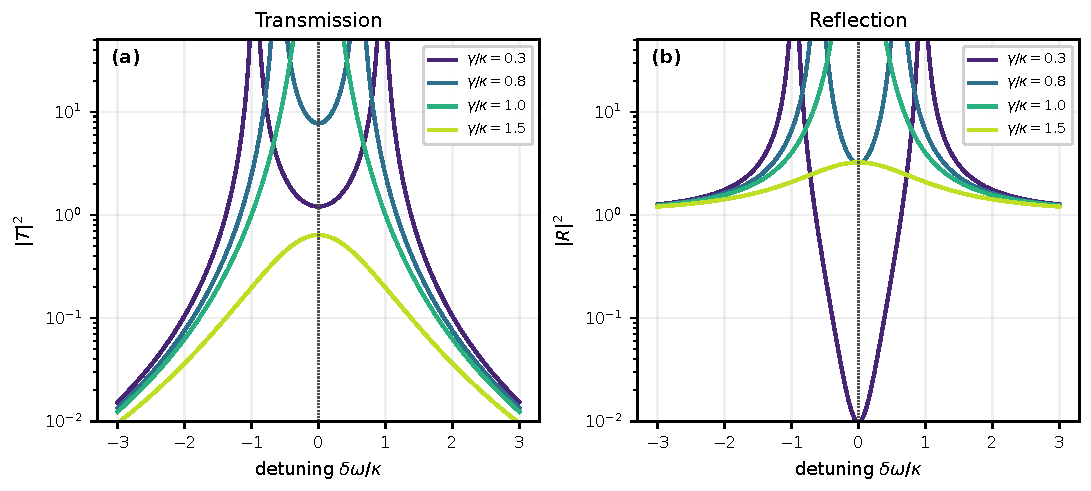
\includegraphics[width=0.95\linewidth]{fig_f9_pt_microring.pdf}
 \caption{Transmission $|T|^2$ and reflection $|R|^2$ of two coupled
 $\PT$-symmetric microring resonators as functions of detuning
 $\delta\omega/\kappa$ for several gain--loss ratios
 $\gamma/\kappa$. Because the system contains gain,
 $|T|^2$ and $|R|^2$ can exceed unity; sharp resonant enhancement near
 $\gamma/\kappa = 1$ marks the exceptional point of the idealized
 two-mode model. In an actual laser, threshold additionally requires a
 scattering pole to reach the real-frequency axis after all intrinsic
 and external losses are included.
 The logarithmic scale reveals qualitatively different lineshapes:
 sub-EP ($\gamma < \kappa$, split peaks), at-EP
 ($\gamma = \kappa$, single divergence), and broken-$\PT$
 ($\gamma > \kappa$, broadened single peak). Dotted vertical
 line marks zero detuning.}
 \label{fig:pt-microring-spectra}
\end{figure}

\begin{booknote}[From models to Maxwell]
Many experimental realizations of $\PT$ symmetry operate in regimes where
the scalar Helmholtz or paraxial approximation is adequate. For
nanophotonic structures where vectorial effects, radiation loss, and
strong dispersion matter, a full Maxwell treatment---returning to the
operator framework of Chapters~\ref{ch:light-eigenvalue}
and~\ref{ch:energy-inner}---is essential. The effective Hamiltonian
description of Chapter~\ref{ch:maxwell-coupled-modes} then provides the
bridge between the full electromagnetics and the $2\times 2$ models.
\end{booknote}


\begin{figure}[t]
 \centering
 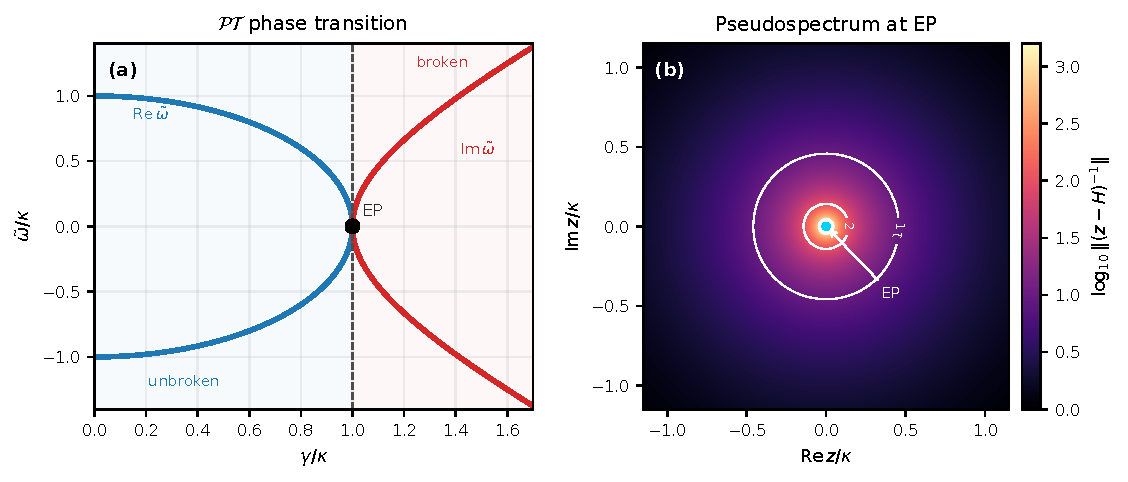
\includegraphics[width=0.97\linewidth]{fig_f9_pt_phase_pseudospectrum.pdf}
 \caption{$\PT$ phase transition and pseudospectrum of the canonical
 $2\times2$ gain--loss Hamiltonian
 $H = \bigl(\begin{smallmatrix} i\gamma & \kappa \\ \kappa & -i\gamma
 \end{smallmatrix}\bigr)$ with $\kappa = 1$.
 (a)~Real (blue) and imaginary (red) parts of the eigenfrequencies
 $\omtil_\pm/\kappa$ as a function of $\gamma/\kappa$. In the
 unbroken phase ($\gamma < \kappa$), both eigenvalues are real:
 $\operatorname{Re}\omtil = \pm\sqrt{1 - \gamma^2/\kappa^2}$. In the
 broken phase ($\gamma > \kappa$), the eigenvalues form a complex
 conjugate pair:
 $\operatorname{Im}\omtil = \pm\sqrt{\gamma^2/\kappa^2 - 1}$. Only
 nonzero branches are plotted; the complementary branch is identically
 zero. The black dot marks the exceptional point at $\gamma = \kappa$.
 (b)~$\varepsilon$-pseudospectrum
 $\log_{10}\|(z - H)^{-1}\|$ at the EP ($\gamma = \kappa$). White
 contour labels give the $\log_{10}$ level. The pseudospectrum bulges
 far from the coalesced eigenvalue at the origin, quantifying the
 system's sensitivity to perturbations
 (Section~\ref{ssec:pt-pseudospectrum}).}
 \label{fig:pt-phase-pseudospectrum}
\end{figure}

%% ================================================================
\section{Non-normality and transient amplification}
\label{sec:pt-nonnormality}

Even in the $\PT$-symmetric phase, where all eigenvalues are real, the
effective Hamiltonian~\eqref{eq:pt-hamiltonian} is non-normal:
$[H_{\PT},\,H_{\PT}^\dagger] \neq 0$. This non-normality has a
physical consequence that is invisible to the eigenvalue spectrum:
\emph{transient amplification} of signals. In the ideal balanced model,
each eigenmode in the exact phase is purely oscillatory, but
non-orthogonal modal superpositions can still grow transiently before
the energy returns to the other quadrature.

\subsection{The mechanism}
\label{ssec:transient-mechanism}

The non-orthogonality of the eigenvectors means that a superposition of
two oscillatory eigenmodes can transiently grow even when both
eigenfrequencies are real. The maximum transient amplification factor is
controlled by the condition number of the eigenvector matrix, which
diverges at the exceptional point.

\paragraph{Example.}
For the $\PT$-symmetric Hamiltonian~\eqref{eq:pt-hamiltonian} with
$\omega_0 = 0$, $\kappa = 1$, and $\gamma = 0.9\kappa$ (deep in the
$\PT$-symmetric phase but close to the EP), the eigenvalues are
$\omtil_\pm = \pm\sqrt{1 - 0.81} = \pm 0.436$. Both eigenvalues are
real, so every eigenmode oscillates without growth. However, the
maximum of $\|e^{-iH_{\PT}t}\|$ over all time is
\begin{equation}
 \max_t \|e^{-iH_{\PT}t}\|
 = \sqrt{\frac{1+\gamma/\kappa}{1-\gamma/\kappa}}
 = \sqrt{\frac{1.9}{0.1}} \approx 4.36.
 \label{eq:transient-max}
\end{equation}
A pulse injected into an optimized superposition of the two cavities can
be amplified by a factor of $4.36$ before the periodic evolution returns
the energy to the other quadrature. At $\gamma/\kappa = 0.99$, this
factor rises to $14.1$; at $\gamma/\kappa = 0.999$, to $44.7$. The
divergence $\propto 1/\sqrt{\kappa - \gamma}$ is a hallmark of
non-normality near an EP.

\subsection{Pseudospectrum}
\label{ssec:pt-pseudospectrum}

The pseudospectrum $\sigma_\epsilon(H)$---the set of complex frequencies
$z$ where $\|(z - H)^{-1}\| > 1/\epsilon$---quantifies the sensitivity
of the spectrum to perturbations. For a normal operator, the
$\epsilon$-pseudospectrum is simply the union of $\epsilon$-discs around
the eigenvalues. For the non-normal $H_{\PT}$, the pseudospectrum
bulges far beyond the eigenvalues into the complex plane, revealing
the system's vulnerability to noise-driven amplification.

For the $\gamma/\kappa = 0.9$ example above, the $\epsilon = 0.1$
pseudospectral boundary extends to $|\Im z| \approx 0.23$, compared to
the eigenvalue imaginary part of exactly zero. This means that an
environmental perturbation of strength $\epsilon = 0.1$ can shift the
effective eigenvalues by $0.23$ in the imaginary direction---more than
twice the perturbation strength---producing transient amplification even
when the unperturbed system is nominally stable.

The pseudospectral viewpoint connects directly to the EP sensing debate
of Chapter~\ref{ch:exceptional-points}: the enhanced responsivity of an
EP sensor is a consequence of the same non-normality that produces
transient amplification and noise enhancement. The Petermann factor
and the maximum transient amplification are closely related measures of
eigenvector non-orthogonality, although they are not identical in
general.


%% ================================================================
\section{Nonlinear $\PT$ symmetry}
\label{sec:pt-nonlinear}

All experimental $\PT$-symmetric systems require gain, and gain media
are inherently nonlinear: at high intensities the gain saturates. This
means that the linear $\PT$-symmetric Hamiltonian is always an
approximation, valid only below the saturation intensity of the gain
medium. Above saturation, the system is described by a nonlinear
$\PT$-symmetric model.

\subsection{Gain saturation and self-consistent $\PT$ symmetry}
\label{ssec:pt-saturation}

The simplest model for gain saturation replaces the constant gain rate
$\gamma$ in~\eqref{eq:pt-hamiltonian} with an intensity-dependent rate
$\gamma(|a|^2) = \gamma_0/(1 + |a|^2/I_{\mathrm{sat}})$, where
$I_{\mathrm{sat}}$ is the saturation intensity. The resulting nonlinear
coupled-mode equations
\begin{equation}
 i\dv{}{t}\begin{pmatrix} a_1 \\ a_2 \end{pmatrix}
 = \begin{pmatrix}
 \omega_0 + i\gamma(|a_1|^2) & \kappa \\
 \kappa & \omega_0 - i\gamma_0
 \end{pmatrix}
 \begin{pmatrix} a_1 \\ a_2 \end{pmatrix}
 \label{eq:pt-nonlinear-eom}
\end{equation}
admit steady-state solutions where the gain self-adjusts to balance the
loss. This \emph{self-consistent} $\PT$ symmetry can be more robust than
the linear version: gain saturation drives the system toward a
gain--loss balance over a finite range of operating conditions
instead of requiring a perfectly fixed small-signal gain
rate~\cite{longhi2018parity,alexeeva2012optical}.

\subsection{Nonlinear exceptional points}
\label{ssec:nonlinear-ep}

Gain saturation modifies the location and character of exceptional
points. In the nonlinear model~\eqref{eq:pt-nonlinear-eom}, the
effective gain rate at steady state is
$\gamma_{\mathrm{eff}} = \gamma_0/(1 + |a_1^{\mathrm{ss}}|^2/I_{\mathrm{sat}})$,
which depends on the solution itself. The EP condition
$\gamma_{\mathrm{eff}} = \kappa$ must therefore be solved
self-consistently: the steady-state intensity determines the gain, which
determines the EP location, which determines the steady-state intensity.

For the two-mode model with $\omega_0 = 0$ and passive loss $\gamma_0$,
the self-consistent EP condition is
\begin{equation}
 \frac{\gamma_0}{1 + |a_1^{\mathrm{ss}}|^2/I_{\mathrm{sat}}} = \kappa,
 \quad\Rightarrow\quad
 |a_1^{\mathrm{ss}}|^2 = I_{\mathrm{sat}}\left(\frac{\gamma_0}{\kappa} - 1\right).
 \label{eq:nonlinear-ep-condition}
\end{equation}
This has a solution only when $\gamma_0 > \kappa$: the \emph{linear}
system is already in the broken phase, but gain saturation pulls the
effective gain back to the EP. The transition can become
\emph{discontinuous} (a first-order phase transition) rather than the
continuous second-order transition of the linear EP, because the
steady-state intensity jumps from zero to a finite value at threshold.

\paragraph{Experimental observations.}
Xia et al.\ demonstrated that local Kerr nonlinearity can tune the
effective gain--loss balance and move the $\PT$ phase boundary, restoring
or destroying topological zero modes in a waveguide
lattice~\cite{xia2021nonlinear}. Wimmer et al.\ observed optical
solitons in $\PT$-symmetric fibre lattices with both globally and locally
$\PT$-symmetric configurations, directly demonstrating that nonlinear
self-trapping can stabilise modes that would be unstable in the linear
broken phase~\cite{wimmer2015observation}. In a complementary theoretical
development, Alexeeva et al.\ analysed soliton families in
$\PT$-symmetric nonlinear couplers and showed that gain saturation
produces symmetric, antisymmetric, and asymmetric soliton branches, with
stability boundaries that are
qualitatively different from the linear EP~\cite{alexeeva2012optical}.

\paragraph{Implications for the linear framework.}
The existence of nonlinear EPs means that the linear non-Hermitian
theory developed in this book is always an approximation for systems
with gain. The approximation is excellent below threshold
($I \ll I_{\mathrm{sat}}$), where $\gamma_{\mathrm{eff}} \approx
\gamma_0$ and the linear EP correctly predicts the phase transition.
Near and above threshold, the nonlinear self-consistency shifts the EP
and can qualitatively change the phase diagram. A complete theory of
non-Hermitian photonics must therefore include the nonlinear regime,
as discussed in Chapter~\ref{ch:open-problems}.

The interplay of nonlinearity and $\PT$ symmetry~\cite{longhi2018parity,hill2026exceptional,bender1998real} connects to the open
problems of Chapter~\ref{ch:open-problems}: the Bogoliubov--de~Gennes
Hamiltonian that governs fluctuations around the nonlinear steady state
is itself non-Hermitian, with a Petermann factor that diverges at the
nonlinear EP. Whether this divergence can be exploited for sensing~\cite{smith2020beyond} or
whether it is always cancelled by noise remains an active research
question.

\chapter{Poles, Zeros, Lasers, and Absorbers}
\label{ch:poles-zeros}

\begin{chapterlead}
The scattering matrix of an optical system encodes every linear response
property---reflection, transmission, absorption, and amplification---as a
function of frequency. Its singularity structure in the complex frequency
plane tells us when the system lases (a pole reaches the real axis), when
it perfectly absorbs (a zero sits on the real axis), and when it does
both simultaneously (the CPA-laser point). This pole--zero description
is used for non-Hermitian photonic systems through concrete examples.
It also establishes the connection between time reversal,
$\PT$ symmetry, and the CPA-laser effect~\cite{novitsky2019cpa,alizadeh2025lasing}, and clarifies the critical
distinctions between exceptional points, CPA-laser thresholds, and
maximum contrast conditions.
\end{chapterlead}


%% ================================================================
\section{Scattering-matrix singularities revisited}
\label{sec:singularities-revisited}

Chapter~\ref{ch:boundaries} introduced the poles and zeros of
$\Smat(\omega)$ as features of the complex frequency plane. We now
develop this picture more systematically.

\subsection{Poles: threshold lasing}
\label{ssec:lasing-poles}

A pole of $\Smat(\omega)$ at $\omtil = \omega_0 - i\gamma$ corresponds to
a quasinormal mode (Chapter~\ref{ch:qnm}). For a passive system,
$\gamma > 0$ and the pole lies below the real axis. If gain is introduced,
$\gamma$ decreases; at threshold, $\gamma \to 0$ and the pole reaches the
real axis:
\begin{equation}
 \Im\,\omtil_n = 0
 \qquad\Longleftrightarrow\qquad
 \text{lasing threshold}.
 \label{eq:lasing-threshold}
\end{equation}
At this point, a self-sustained oscillation exists at real frequency
$\omega_0$ with no external driving---the system is a laser.

The physical picture is transparent in the pole--zero language: gain lifts
the QNM poles toward the real axis. A passive cavity has all poles in the
lower half-plane; adding gain is equivalent to reducing the imaginary parts
of the poles. The first pole to reach the real axis sets the lasing
threshold and frequency.

\subsection{Zeros: coherent perfect absorption}
\label{ssec:cpa-zeros}

A zero of $\det\Smat(\omega)$ at real $\omega$ means there exists a
specific combination of incoming waves such that the outgoing field
vanishes identically. All incident energy is absorbed. This is
\emph{coherent perfect absorption} (CPA)~\cite{chong2010symmetry}.

CPA requires precise control of the relative phase and amplitude of the
incoming beams. For a two-port system, the CPA condition is
\begin{equation}
 \det\Smat(\omega_{\mathrm{CPA}}) = 0
 \quad\Longleftrightarrow\quad
 \text{an eigenvalue of } \Smat \text{ vanishes}.
 \label{eq:cpa-condition}
\end{equation}

\subsection{The meromorphic structure}
\label{ssec:meromorphic}

The scattering matrix $\Smat(\omega)$ of a finite photonic structure is a
meromorphic function of $\omega$: it is analytic everywhere in the complex
plane except at isolated poles. Any meromorphic matrix can be written in
terms of its poles and zeros as a product expansion. For a scalar
reflection or transmission coefficient $s(\omega)$, this takes the form
\begin{equation}
 s(\omega) = A\,\prod_j \frac{\omega - z_j}{\omega - p_j},
 \label{eq:pole-zero-product}
\end{equation}
where $\{p_j\}$ are the poles, $\{z_j\}$ are the zeros, and $A$ is a
constant prefactor. This representation makes the spectral response a
direct map of the singularity positions:
\begin{itemize}
 \item Near a pole $p_j$, the response $|s(\omega)|^2$ diverges---a
 sharp amplification peak.
 \item Near a zero $z_j$, the response vanishes---a sharp absorption dip.
 \item Between a nearby pole--zero pair, the response exhibits a Fano
 line shape: asymmetric with a rapid transition from absorption to
 amplification.
\end{itemize}


%% ================================================================
\section{Example: Fabry--P\'erot cavity}
\label{sec:fabry-perot-poles}

The Fabry--P\'erot cavity is the simplest photonic structure that
illustrates the full pole--zero framework.

\subsection{Setup and transfer matrix}
\label{ssec:fp-setup}

Consider a dielectric slab of thickness $L$, refractive index
$n = n' + in''$ (with $n'' > 0$ for loss and $n'' < 0$ for gain),
embedded in vacuum. The transfer matrix for the slab, including the two
air--dielectric interfaces, is (Appendix~\ref{app:transfer})
\begin{equation}
 \Tmat = \frac{1}{4n}\begin{pmatrix}
 (n+1)^2 e^{-i\phi} - (n-1)^2 e^{i\phi} & (n^2-1)(e^{i\phi}-e^{-i\phi}) \\
 (n^2-1)(e^{-i\phi}-e^{i\phi}) & (n+1)^2 e^{i\phi} - (n-1)^2 e^{-i\phi}
 \end{pmatrix},
 \label{eq:fp-transfer}
\end{equation}
where $\phi = n\omega L/c$ is the single-pass phase. The transmission
coefficient is $t = 1/T_{22}$.

\subsection{Pole positions}
\label{ssec:fp-poles}

The poles of $t(\omega)$ are the zeros of $T_{22}$, which satisfy the
round-trip resonance condition
\begin{equation}
 r_{12}^2\,e^{-2in\omega L/c} = 1,
 \label{eq:fp-roundtrip}
\end{equation}
where $r_{12} = (n-1)/(n+1)$ is the Fresnel reflection coefficient at
each interface. For weak material loss or gain, write
$r_{12} \approx |r_{12}|\,e^{i\varphi_r}$ using the real background
index $n'$. The pole frequencies are then approximately
\begin{equation}
 \omtil_m \approx \frac{c}{n' L}\bigl(m\pi - \varphi_r\bigr)
 - i\,\frac{c}{n' L}\,\ln\frac{1}{|r_{12}|},
 \qquad m = 0, \pm 1, \pm 2, \ldots
 \label{eq:fp-poles}
\end{equation}
For the lossless reference cavity, the imaginary part is negative: all
poles lie below the real axis. The mirror-limited decay rate is
$\gamma_m = (c/n'L)\ln(1/|r_{12}|)$; material absorption adds to this
decay, while material gain subtracts from it.

\paragraph{Counting poles and zeros.}
For the Fabry--P\'erot slab, the poles and zeros of the scalar
transmission $t(\omega)$ are approximately equally spaced in the complex
plane with a free spectral range $\Delta\omega = \pi c/(n'L)$ when the
dispersion and absorption are weak. In the lossless reference cavity,
zeros are the time reverses of the poles and appear at the conjugate
positions. Material loss or gain moves the zeros as well as the poles;
the zero motion is what makes coherent perfect absorption possible.

For a slab with $n' = 3.5$ and $L = 300\;$nm at telecom wavelengths
($\lambda \sim 1550\;$nm), the free spectral range is
$\Delta\omega \approx 4.49 \times 10^{14}\;$rad/s, and the Fresnel
reflectivity $|r_{12}|^2 = [(3.5-1)/(3.5+1)]^2 \approx 0.309$ gives
a quality factor $Q = \omega_0/(2\gamma_0) \approx 2.7$
for the lowest-order mode. The low $Q$ makes the pole--zero structure
well separated and easy to resolve, which is why this cavity is ideal
for pedagogical demonstration of the scattering singularity framework.

\subsection{Adding gain: pole motion toward lasing}
\label{ssec:fp-gain}

If the slab material has gain ($n'' < 0$), the imaginary part of the
propagation phase $\phi$ acquires a positive contribution that
counteracts the mirror loss. The pole frequency becomes
\begin{equation}
 \Im\,\omtil_m = -\frac{c}{n'L}\bigl[\ln(1/|r_{12}|) + n''\omega_m L/c\bigr].
 \label{eq:fp-pole-gain}
\end{equation}
When $|n''|\omega_m L/c = \ln(1/|r_{12}|)$, the imaginary part vanishes
and the pole reaches the real axis: this is the lasing threshold for mode
$m$. The threshold gain is
\begin{equation}
 g_{\mathrm{th}} = \frac{2\ln(1/|r_{12}|)}{L},
 \label{eq:fp-threshold}
\end{equation}
where $g_{\mathrm{th}} = 2|n''|\omega/c$ is the power gain coefficient.
This is the standard textbook result, but here it emerges naturally as a
statement about pole motion in the complex plane.

\subsection{Zero positions and CPA}
\label{ssec:fp-zeros}

The zeros of $\det\Smat$ for the Fabry--P\'erot slab satisfy the
time-reversed round-trip condition:
\begin{equation}
 r_{12}^{*2}\,e^{-2in^*\omega L/c} = 1.
 \label{eq:fp-zero-condition}
\end{equation}
For a purely lossy slab ($n'' > 0$), the zeros lie in the upper
half-plane. As loss increases, zeros descend toward the real axis.
CPA occurs when a zero reaches the real axis: the slab absorbs all
coherently incident light at the CPA frequency.

The CPA threshold loss is the mirror image of the lasing threshold gain:
\begin{equation}
 \alpha_{\mathrm{CPA}} = \frac{2\ln(1/|r_{12}|)}{L},
 \label{eq:fp-cpa-threshold}
\end{equation}
confirming the time-reversal duality~\cite{sweeney2019perfectly,wang2021coherent}: CPA is lasing run backward.

\paragraph{Explicit pole--zero map for the Fabry--P\'erot cavity.}
For the $n' = 3.5$, $L = 300\;$nm slab, the first three poles are at
$\omtil_m/\Delta\omega = m - i\,0.187$ for $m = 1, 2, 3$, and the
corresponding zeros at $\omtil_m^*/\Delta\omega = m + i\,0.187$. As
gain is added ($n'' \to -|n''|$), each pole moves vertically upward by
$\delta(\Im\omtil) = |n''|\omega_m/n'$. The lasing threshold for
mode $m$ is $|n''|_{\mathrm{th}} = \ln(1/|r_{12}|)\,c/(\omega_m L)
= 0.187\,\Delta\omega/\omega_m$. Simultaneously, each zero moves
downward by the same amount---the gain that brings a pole to the real
axis pushes its partner zero away. Only in a $\PT$-symmetric
configuration (gain and loss in separate halves of the cavity) do a
pole and zero converge on the real axis simultaneously, producing the
CPA-laser point.

%% ================================================================
\section{Time reversal and the CPA-laser duality}
\label{sec:time-reversal}

CPA and lasing are connected by time reversal. A laser emits coherent
radiation with no input; CPA absorbs coherent radiation with no output.
Formally, if $\Smat(\omega_L)$ has a pole (lasing), then
$\Smat^{-1}(\omega_L)$ has a zero---and $\Smat^{-1}$ is the scattering
matrix of the time-reversed system (with gain and loss
exchanged)~\cite{chong2010symmetry}.

\subsection{Formal statement}
\label{ssec:tr-formal}

Let $\Smat(\omega)$ be the scattering matrix of a linear system with
material parameters $\epsr(\rr)$. The time-reversed system has
$\varepsilon_{\mathrm{TR}}(\rr) = \epsr^*(\rr)$ (gain $\leftrightarrow$ loss),
and its scattering matrix is
\begin{equation}
 \Smat_{\mathrm{TR}}(\omega) = [\Smat(\omega^*)]^{*\,-1}.
 \label{eq:s-time-reversed}
\end{equation}
At real frequencies, $\Smat_{\mathrm{TR}}(\omega) = [\Smat(\omega)]^{-1\,*}$.
The poles of $\Smat$ become zeros of $\Smat_{\mathrm{TR}}$, and vice versa.

\subsection{CPA-laser point}
\label{ssec:cpa-laser}

For a system with both gain and loss, lasing and CPA can occur at the
\emph{same} frequency if and only if a pole and a zero of $\Smat$
coincide on the real axis. This simultaneous occurrence is the
\emph{CPA-laser} point.

A $\PT$-symmetric structure provides a natural setting for the CPA-laser
because the $\PT$ constraint relates the inverse scattering matrix to
the parity-transformed, time-reversed scattering matrix. For real
frequencies this is the two-port relation discussed in
Chapter~\ref{ch:pt-symmetric}; analytically continued into the complex
plane, it pairs a pole at $\omtil$ with a zero at $\omtil^*$.
When $\omtil$ reaches the real axis, the pole and zero meet
simultaneously---the CPA-laser condition is automatically satisfied.

%% ================================================================
\section{$\PT$-symmetric scattering}
\label{sec:pt-scattering}

For a $\PT$-symmetric structure, the scattering matrix satisfies the
fundamental relation~\eqref{eq:pt-s-relation}. At real frequencies, the
consequences are:
\begin{enumerate}
 \item $|\det\Smat| = 1$: the product of scattering eigenvalues has
 unit modulus.
 \item Poles and zeros of $\Smat$ come in conjugate pairs:
 if $\omtil$ is a pole, then $\omtil^*$ is a zero, and vice versa.
 \item In the $\PT$-symmetric phase, both scattering eigenvalues are
 unimodular: neither net amplification nor net absorption occurs.
 \item In the $\PT$-broken phase, one eigenvalue has $|s| > 1$
 (amplification) and the other has $|s| < 1$ (absorption).
\end{enumerate}

The CPA-laser point, where a pole and zero meet on the real axis,
corresponds to the special situation where $\PT$ symmetry enforces
$s_1 \to \infty$ and $s_2 \to 0$ simultaneously, keeping
$|s_1 s_2| = 1$.

\subsection{Scattering phase diagram}
\label{ssec:scattering-phase-diagram}

As the gain--loss parameter $\gamma$ increases from zero, the scattering
eigenvalues trace paths in the complex plane. Three qualitatively
different regimes emerge:
\begin{enumerate}
 \item \textbf{$\PT$-symmetric phase ($\gamma < \gamma_{\mathrm{EP}}$):}
 both $|s_1| = |s_2| = 1$. The system is transparent on average,
 though phase shifts differ from the passive case.
 \item \textbf{$\PT$-broken phase ($\gamma_{\mathrm{EP}} < \gamma < \gamma_{\mathrm{CPA}}$):}
 $|s_1| > 1$, $|s_2| < 1$. One channel amplifies, the other absorbs,
 but neither diverges.
 \item \textbf{CPA-laser threshold ($\gamma = \gamma_{\mathrm{CPA}}$):}
 $|s_1| \to \infty$, $|s_2| \to 0$. The system simultaneously lases
 and perfectly absorbs at the same frequency for different input states.
\end{enumerate}
This phase diagram highlights that the EP (a spectral degeneracy) and
the CPA-laser (a pole--zero coincidence) generally occur at
\emph{different} gain--loss values.

%% ================================================================
\section{Transfer-matrix analysis of a $\PT$ multilayer}
\label{sec:pt-multilayer}

\subsection{Setup}
\label{ssec:multilayer-setup}

Consider a multilayer stack of $N$ unit cells, each composed of a loss
layer (thickness $d_1$, refractive index $n_1 = n_0 + i\kappa_I$) and a
gain layer (thickness $d_2 = d_1$, refractive index
$n_2 = n_0 - i\kappa_I$). This structure satisfies the $\PT$ condition
$n(x) = n^*(-x)$ when the inversion center is placed at the interface
between the loss and gain layers.

\subsection{Output coefficients}
\label{ssec:output-coefficients}

The total transfer matrix $\Tmat^N$ determines the reflection and
transmission through~\eqref{eq:pt-transfer-to-scatter}. As a function of
the gain--loss parameter $\kappa_I$, three regimes
emerge~\cite{novitsky2019cpa}:
\begin{enumerate}
 \item \textbf{Below the EP} ($\kappa_I < \kappa_{\mathrm{EP}}$):
 the transmission and reflection show moderate asymmetry. The output
 intensity can exceed the input, but the contrast between amplification
 and absorption is limited.
 \item \textbf{At the EP} ($\kappa_I = \kappa_{\mathrm{EP}}$):
 the transfer-matrix eigenvalues coalesce. The output exhibits maximum
 contrast between amplification and absorption for specific input
 configurations.
 \item \textbf{Above the EP} ($\kappa_I > \kappa_{\mathrm{EP}}$):
 the system enters the $\PT$-broken phase. One scattering channel
 grows exponentially with $N$ (laser-like amplification), while the
 other is exponentially suppressed (CPA-like absorption).
\end{enumerate}

\subsection{CPA-laser versus exceptional point}
\label{ssec:cpa-vs-ep}

A common misconception is that the CPA-laser point coincides with the
exceptional point. In general, it does not~\cite{novitsky2019cpa}.
The EP is a property of the transfer matrix eigenvalues (a spectral
degeneracy); the CPA-laser is a property of the scattering matrix
singularities (a pole--zero coincidence on the real axis). The two
conditions are related but distinct:
\begin{itemize}
 \item The EP can occur at a gain--loss value where no real-frequency
 pole or zero exists.
 \item The CPA-laser point can occur in the broken phase, away from
 the EP.
 \item Maximum output contrast (the ratio of amplification to
 absorption for different input phases) need not coincide with
 either the EP or the CPA-laser point.
\end{itemize}

This distinction is physically important: the EP controls the spectral
topology and the eigenvector structure, while the CPA-laser controls the
input--output energy balance.

\begin{takeaway}[Three distinct critical points]
In a $\PT$-symmetric scattering system, the exceptional point (spectral
degeneracy), the CPA-laser point (pole--zero coincidence), and the point
of maximum amplification--absorption contrast are in general three
different parameter values. Conflating them leads to incorrect
predictions of device performance.
\end{takeaway}


%% ================================================================
\section{Spectral singularities}
\label{sec:spectral-singularities}

\subsection{Definition}
\label{ssec:spectral-sing-def}

A \emph{spectral singularity} is a point on the real frequency axis~\cite{longhi2010mml,chong2010symmetry}
where the reflection or transmission coefficient diverges---i.e., a pole
of $\Smat(\omega)$ at real $\omega$. Unlike the QNM poles discussed
above, which lie in the lower half-plane for passive systems, a spectral
singularity occurs on the real axis and is the scattering-theory
description of threshold lasing in a linear gain medium.

Mathematically, a spectral singularity at $\omega_s$ means the
resolvent of the Maxwell operator is unbounded at $\omega_s$, but
$\omega_s$ is not an eigenvalue in the standard sense: no
square-integrable eigenfunction exists. Instead, a spectral singularity
is a divergence of the scattering amplitude at a real frequency---an
``eigenvalue embedded in the continuum'' of the non-self-adjoint
operator.

\subsection{Physical interpretation}
\label{ssec:spectral-sing-physics}

For optical systems, spectral singularities have two complementary
physical manifestations that are connected by time reversal.

The first is \emph{lasing}. A pole of $\Smat(\omega)$ on the real
axis means that the system sustains a self-oscillating field at
frequency $\omega_s$ without any external drive. In the meromorphic
representation
\begin{equation}
 \Smat(\omega) = \Smat_{\mathrm{bg}}(\omega)\,
 \prod_n \frac{\omega - z_n}{\omega - p_n},
 \label{eq:smat-meromorphic}
\end{equation}
where $p_n$ are the QNM poles and $z_n$ the scattering zeros, lasing
occurs when one pole $p_m$ migrates to the real axis:
$\Im\,p_m \to 0^-$. At this point the denominator
$(\omega - p_m)$ vanishes for real $\omega = \Re\,p_m$, and the
scattering amplitudes diverge. The outgoing field grows without bound
in time---the signature of stimulated emission overcoming all losses.

The second manifestation is \emph{coherent perfect absorption} (CPA),
also called anti-lasing. A zero of $\det\Smat(\omega)$ on the real
axis means that there exists a coherent input field configuration that
is perfectly absorbed: no light exits the structure. Mathematically,
this is a spectral singularity of the \emph{inverse} scattering matrix
$\Smat^{-1}$. By~\eqref{eq:smat-meromorphic}, CPA occurs when a zero
$z_m$ sits on the real axis: $\Im\,z_m = 0$.

The connection between lasing and CPA follows from the time-reversal
structure of the S-matrix. A pole of a given system maps to a zero of
the time-reversed system, in which gain and loss are interchanged. In a
lossless reciprocal reference problem this reduces to the familiar
conjugate pole--zero symmetry, but it is not a general consequence of
reciprocity alone. In specially constrained active systems, most notably
$\PT$-symmetric ones, a pole and a zero can be forced to reach the real
axis together. This is the \emph{CPA-laser}
point~\cite{chong2010symmetry,sweeney2019perfectly}, at which the system
can act as either a laser or a perfect absorber depending on the input
coherence.

\paragraph{Quantitative threshold from S-matrix poles.}
Combining the meromorphic representation~\eqref{eq:smat-meromorphic}
with the Fabry--P\'erot pole positions from
Section~\ref{ssec:fp-poles}, the lasing threshold for mode $m$ is
reached when the gain $g$ satisfies
\begin{equation}
 g = g_{\mathrm{th},m}
 = -\frac{2\,\Im\,p_m(g=0)}{c/n_g}
 = \frac{2\ln(1/|r_{12}|)}{L}
 + \alpha_{\mathrm{mat}},
 \label{eq:threshold-from-poles}
\end{equation}
where $n_g$ is the group index, $\alpha_{\mathrm{mat}}$ accounts for
material absorption, and $|r_{12}|$ is the mirror reflectivity. The
first term is the mirror loss and the second the material loss; the
threshold condition requires the gain to compensate both. This
derivation makes explicit the pole-motion picture: gain ``lifts'' the
pole at a rate $c\,g/(2n_g)$ until it reaches the real axis.

\subsection{Threshold condition as a spectral singularity}
\label{ssec:spectral-threshold}

The spectral-singularity viewpoint provides a precise mathematical
criterion for the lasing threshold that goes beyond the simple
$\Im\omtil = 0$ condition. For a one-dimensional potential
$V(x) = -\omega^2[\varepsilon(x) - 1]/c^2$ with complex $\varepsilon$,
the spectral singularity occurs when the Jost function $f^+(\omega)$
vanishes at a real $\omega$ while $f^-(\omega) \neq 0$. This is a
stronger condition than a pole of the reflection coefficient: it
requires that the outgoing-wave solution be bounded (not
square-integrable) while the incoming-wave solution diverges.

For the Fabry--P\'erot cavity, the Jost-function condition reduces to
the round-trip condition~\eqref{eq:fp-roundtrip} evaluated on the real
axis. But for more complex structures---photonic crystals, coupled
resonators, random media---the Jost-function framework provides a
rigorous definition of the lasing threshold that does not require
identifying individual QNM poles.

\subsection{Spectral singularities in $\PT$-symmetric potentials}
\label{ssec:spectral-sing-pt}

In a $\PT$-symmetric optical potential, spectral singularities have
special properties. For reciprocal one-dimensional scattering, the
generalized conservation relation can be written as
\begin{equation}
 \bigl||t(\omega)|^2-1\bigr|=\sqrt{R_L(\omega)R_R(\omega)},
 \qquad R_{L,R}=|r_{L,R}|^2 .
 \label{eq:pt-generalized-unitarity}
\end{equation}
A spectral singularity at $\omega_s$ corresponds to
 $|t(\omega_s)| \to \infty$, and the reflection product diverges
simultaneously---the system emits coherent radiation into the available
channels. Its time-reversed partner is the CPA condition.


%% ================================================================
\section{Beyond $\PT$: general pole--zero engineering}
\label{sec:pole-zero-engineering}

The pole--zero framework extends beyond $\PT$-symmetric systems. For
any linear photonic structure described by a scattering matrix, the
motion of poles and zeros in the complex frequency plane under parameter
changes follows simple rules that enable systematic device design.
Gain moves poles upward in the complex plane, toward the real axis and
eventually through it to lasing. Loss moves poles downward, increasing
decay rates and broadening resonances. Structural changes---geometry,
coupling strength, grating period---move poles horizontally, shifting
the resonance frequency while leaving the decay rate largely unchanged.
The zero structure is constrained by causality, time-reversal relations,
and passivity bounds on real-frequency scattering, but zeros are not
fixed by reciprocity alone. Indeed, in passive absorbers one deliberately
moves a scattering zero onto the real axis by controlling the spatial
profile and strength of absorption.
These rules provide an intuitive design language: achieving CPA at a
target frequency amounts to placing a zero on the real axis, while
suppressing a parasitic lasing mode amounts to pushing its pole deeper
into the lower half-plane.

\subsection{Design as singularity placement}
\label{ssec:design-singularity}

Designing a photonic device---a laser, a sensor, a filter, or an
absorber---can be viewed as engineering the positions of poles and zeros
in the complex frequency plane to achieve the desired spectral response.
This perspective unifies many seemingly different problems:
\begin{itemize}
 \item A narrow-band laser requires one pole close to the real axis with
 all other poles far away.
 \item A broadband absorber requires zeros spread along the real axis.
 \item A Fano resonance requires a nearby pole--zero pair with
 controlled spacing.
 \item A flat-top filter requires poles and zeros arranged in a
 Butterworth-like pattern.
\end{itemize}

\paragraph{Metasurface example: pole--zero placement for perfect
absorption.}
Consider a metasurface consisting of a periodic array of lossy
dielectric resonators on a metallic back-reflector. The back-reflector
eliminates transmission, so the scattering problem reduces to a
single-port reflection coefficient $r(\omega)$. Perfect absorption at
a target frequency $\omega_0$ requires $r(\omega_0) = 0$, i.e., a zero
of $r$ on the real axis. In the pole--zero language, this is achieved
by tuning the resonator geometry so that a pole at
$\omtil = \omega_0 - i\gamma$ is paired with a zero at
$z = \omega_0 + i\gamma'$, and then adjusting the material loss so
that $\gamma' \to 0$. The critical-coupling condition
$\gamma_{\mathrm{rad}} = \gamma_{\mathrm{abs}}$ (radiative decay
equals absorptive decay) is precisely the statement that the zero
reaches the real axis.

With the global $e^{-i\omega t}$ convention used in this book, a
one-port temporal coupled-mode model may be written in the dimensionless
form
\begin{equation}
 r(\Delta)=
 \frac{-i\Delta+\gamma_{\mathrm{abs}}-\gamma_{\mathrm{rad}}}
 {-i\Delta+\gamma_{\mathrm{abs}}+\gamma_{\mathrm{rad}}},
 \qquad \Delta=\omega-\omega_0.
 \label{eq:one-port-critical-coupling}
\end{equation}
The pole and zero are therefore
\begin{equation}
 \omega_p=\omega_0-i(\gamma_{\mathrm{abs}}+\gamma_{\mathrm{rad}}),
 \qquad
 \omega_z=\omega_0+i(\gamma_{\mathrm{rad}}-\gamma_{\mathrm{abs}}).
 \label{eq:one-port-pole-zero}
\end{equation}
The passive zero starts in the upper half-plane when absorption is weak
and crosses the real axis at critical coupling.

\begin{figure}[t]
 \centering
 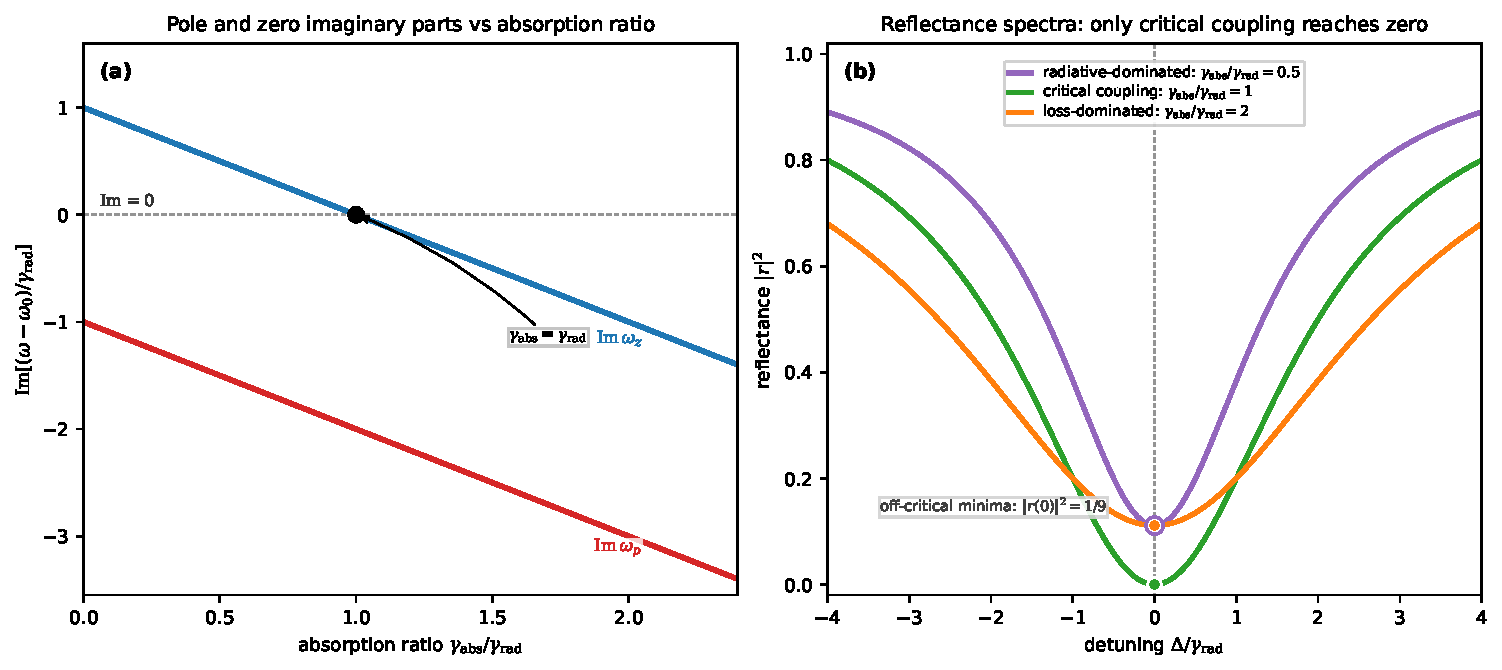
\includegraphics[width=0.96\linewidth]{fig_f10_critical_coupling_absorber.pdf}
 \caption{Critical coupling as zero placement in a one-port absorber.
 The time convention is $e^{-i\omega t}$ and the reflection amplitude is
 Eq.~\eqref{eq:one-port-critical-coupling}. (a)~Imaginary parts of
 the pole and zero in Eq.~\eqref{eq:one-port-pole-zero} as the ratio
 $\gamma_{\mathrm{abs}}/\gamma_{\mathrm{rad}}$ is varied. The pole
 remains in the lower half-plane, while the passive zero begins in the
 upper half-plane and reaches $\operatorname{Im}\omega_z=0$ at
 $\gamma_{\mathrm{abs}}=\gamma_{\mathrm{rad}}$. (b)~Real-frequency
 reflectance spectra for under-coupled
 ($\gamma_{\mathrm{abs}}/\gamma_{\mathrm{rad}}=0.5$), critically
 coupled, and over-coupled
 ($\gamma_{\mathrm{abs}}/\gamma_{\mathrm{rad}}=2$) cases. The two
 off-critical spectra have the same minimum reflectance,
 $|r(0)|^2=1/9$, while critical coupling gives $|r(0)|^2=0$.}
 \label{fig:ch10-critical-coupling-absorber}
\end{figure}

This design recipe generalises to multi-frequency perfect absorption:
each target frequency requires one zero on the real axis, which in turn
requires one resonator mode with matched radiative and absorptive
decay rates. The pole--zero framework provides a systematic way to
count the degrees of freedom and identify the minimum number of
resonator modes needed for a given absorption bandwidth.

There is an important physical distinction between critical coupling and
lasing threshold. Critical coupling is still a passive condition: the
pole remains in the lower half-plane because
$\operatorname{Im}\omega_p=-(\gamma_{\mathrm{abs}}+
\gamma_{\mathrm{rad}})<0$. The device absorbs perfectly at one real
frequency not because the stored field grows without bound, but because
the directly reflected wave and the field re-radiated by the resonator
cancel exactly in the outgoing channel. In Maxwell language, the
Poynting flux entering the resonator through the external channel equals
the Ohmic or material-loss power dissipated inside the resonator. This
is why the condition is often called \emph{impedance matching}: the
external radiation resistance and internal absorption resistance are
matched.

This clarification prevents a common misconception. Moving a zero to
the real axis is not the same as moving a pole to the real axis. The
first produces a finite, stable absorbing solution for a particular
coherent input; the second produces a self-sustained outgoing solution
with no input. The two events can coincide only in special active
systems such as the $\PT$-symmetric CPA-laser discussed above. In a
one-port passive metasurface, only the zero reaches the real axis, so
perfect absorption is compatible with stability, causality, and finite
stored energy.

\subsection{Passivity constraints}
\label{ssec:passivity-poles}

For a passive system (no gain), the poles of $\Smat(\omega)$ must lie in
the lower half-plane. This is a direct consequence of causality and
stability: the Green function of a passive system decays in the future,
not the past. Scattering zeros obey different constraints. In a lossless
unitary system they mirror the poles across the real axis; in a lossy
passive system they can move onto the real axis, producing CPA, or away
from the simple conjugate locations. Violating pole stability requires
gain, which is the fundamental reason why lasers and CPA-lasers are
active devices.

\subsection{Connection to QNM perturbation theory}
\label{ssec:pole-zero-qnm}

The biorthogonal perturbation theory of Chapter~\ref{ch:qnm} provides
the sensitivity of pole positions to material or geometric changes:
\begin{equation}
 \delta\omtil_n = -\frac{\omtil_n}{2}
 \frac{\int \delta\epsr\,\tilde{\EE}_n\cdot\tilde{\EE}_n\;\dd^3r}
 {\mathcal{N}_n}.
 \label{eq:pole-shift-perturbation}
\end{equation}
Here $\mathcal{N}_n$ is the unconjugated QNM normalization, including the
appropriate dispersive and surface or PML contribution. This formula
directly connects the pole--zero engineering picture to the underlying
Maxwell fields: placing gain where the relevant QNM has large overlap
moves the pole most efficiently toward the real axis.


%% ================================================================
\section{Connections}
\label{sec:ch10-forward}

This closes the scattering part of the book. Exceptional points,
$\PT$-symmetric optics, and pole--zero motion describe complementary
aspects of non-Hermitian photonic systems driven by gain, loss, and
coupling.

Part~IV now turns to the topological structure of non-Hermitian photonic
bands. Chapter~\ref{ch:berry-maxwell} builds Berry curvature directly
from Maxwell fields; Chapter~\ref{ch:complex-bands} introduces complex
bands and non-Hermitian gaps; and the subsequent chapters develop the
photonic skin effect, point-gap topology, and the reconstruction of
bulk-boundary correspondence.


% ════════════════════════════════════════════════════════════
% PART IV — Topology Before and After Hermiticity
% ════════════════════════════════════════════════════════════
\part{Topology Before and After Hermiticity}

\chapter{Berry Curvature from Maxwell Fields}
\label{ch:berry-maxwell}

\begin{chapterlead}
Topology entered condensed-matter physics through the Berry phase of
electronic Bloch states. The same mathematics applies to photonic Bloch
modes---but with an important difference: the inner product is defined by
the electromagnetic energy, not by the probability density. This chapter
derives Berry connection, Berry curvature, and Chern numbers directly from
the Maxwell eigenproblem, without passing through a tight-binding analogy.
The result is a Maxwell-first topological photonics that connects the
band structure of Chapter~\ref{ch:periodicity} to the existence of
topologically protected edge states.
\end{chapterlead}


%% ================================================================
\section{Why the inner product matters}
\label{sec:inner-product-matters}

Before computing the Berry phase, we must settle a question that has no
analogue in electronic topological insulators: \emph{which inner product
defines the Berry connection?}

In quantum mechanics, the choice is unambiguous: the standard
$L^2$ inner product $\langle\psi|\phi\rangle = \int\psi^*\phi\;\dd^3r$.
In photonics, the natural inner product comes from the electromagnetic
energy density. For nondispersive Hermitian media, the $\EE$-field
formulation uses the weighted product
\begin{equation}
 \langle\mathbf{u}|\mathbf{v}\rangle_\varepsilon
 = \int_{\Omega_{\mathrm{uc}}}
 \epsr(\rr)\,\mathbf{u}^*(\rr)\cdot\mathbf{v}(\rr)\;\dd^d r,
 \label{eq:eps-inner}
\end{equation}
while for the $\HH$-field formulation with $\mur=1$ it is the unweighted
form
\begin{equation}
 \langle\mathbf{u}|\mathbf{v}\rangle
 = \int_{\Omega_{\mathrm{uc}}}
 \mathbf{u}^*(\rr)\cdot\mathbf{v}(\rr)\;\dd^d r.
 \label{eq:h-inner}
\end{equation}
The $\HH$-field formulation leads to the Hermitian eigenoperator
$\hat{\Theta}_H = \curl\bigl(\epsr^{-1}\curl\,\cdot\,\bigr)$ whose
eigenstates are automatically orthogonal in~\eqref{eq:h-inner}. The
$\EE$-field formulation leads to a generalized eigenproblem
$\curl(\mur^{-1}\curl\EE) = (\omega^2/c^2)\epsr\EE$ whose eigenstates
are orthogonal in the $\epsr$-weighted product~\eqref{eq:eps-inner}.

Both formulations give the same Berry curvature and Chern numbers when
$\epsr$ is Hermitian (real for scalar, Hermitian for tensor), because
the eigenstates are related by a gauge transformation. However, the
$\epsr$-weighted inner product is the physically correct one for
perturbation theory, for normalization of mode amplitudes, and for the
construction of Wannier functions~\cite{paz2019tutorial}. In dispersive
but lossless media, $\epsr$ is replaced by the Brillouin energy weight
discussed in Chapter~\ref{ch:loss-gain-dispersion}.

\begin{remark}
In non-Hermitian systems (complex $\epsr$), the two formulations lead
to different Berry connections because the $\epsr$-weighted inner
product is no longer positive definite. The resolution requires the
biorthogonal Berry connection of Section~\ref{sec:nh-berry-preview} and
Chapter~\ref{ch:complex-bands}.
\end{remark}


%% ================================================================
\section{Geometric phase for photonic Bloch states}
\label{sec:berry-photonic}

Recall from Chapter~\ref{ch:periodicity} that the Bloch eigenmodes of a
periodic photonic crystal satisfy the unit-cell eigenproblem
$\Mop_\kk\,\mathbf{u}_{n\kk} = (\omega_n(\kk)^2/c^2)\,\mathbf{u}_{n\kk}$,
with $\mathbf{u}_{n\kk}(\rr)$ periodic on $\Omega_{\mathrm{uc}}$.
As $\kk$ varies over the Brillouin zone, $\mathbf{u}_{n\kk}$ traces a
path in the Hilbert space of periodic vector fields. The geometric phase
accumulated along this path is the photonic Berry phase.

\subsection{Berry connection}
\label{ssec:berry-connection}

The \emph{Berry connection} for band $n$ is the one-form on the
Brillouin zone defined by~\cite{paz2019tutorial}
\begin{equation}
 \Acal_{n,\alpha}(\kk) = i\,
 \frac{\langle\mathbf{u}_{n\kk}|\partial_{k_\alpha}|\mathbf{u}_{n\kk}\rangle_\varepsilon}
 {\langle\mathbf{u}_{n\kk}|\mathbf{u}_{n\kk}\rangle_\varepsilon},
 \label{eq:berry-connection}
\end{equation}
where $\alpha = x, y$ labels the components of $\kk$ and the inner
product is the $\epsr$-weighted form~\eqref{eq:eps-inner}. When the
modes are normalized to
$\langle\mathbf{u}_{n\kk}|\mathbf{u}_{n\kk}\rangle_\varepsilon = 1$,
the denominator drops out.

The Berry connection is \emph{gauge-dependent}: under a gauge
transformation $|\mathbf{u}_{n\kk}\rangle \to e^{i\phi(\kk)}|\mathbf{u}_{n\kk}\rangle$,
it shifts by $\Acal_{n,\alpha} \to \Acal_{n,\alpha} - \partial_{k_\alpha}\phi$. Physical
observables must therefore depend on gauge-invariant combinations.

\subsection{Berry curvature}
\label{ssec:berry-curvature}

The \emph{Berry curvature} is the gauge-invariant curl of the Berry
connection. In two dimensions ($\kk = (k_x,k_y)$), it is a
pseudoscalar:
\begin{equation}
 \Fcal_n(\kk) = \pdv{\Acal_{n,y}}{k_x} - \pdv{\Acal_{n,x}}{k_y}.
 \label{eq:berry-curvature-2d}
\end{equation}
An equivalent expression that does not require differentiating the
Berry connection directly is the Kubo-like formula:
\begin{equation}
 \Fcal_n(\kk) = -2\sum_{m\neq n}
 \frac{\Im\bigl[
 \langle\mathbf{u}_{n\kk}|\partial_{k_x}\Mop_\kk|\mathbf{u}_{m\kk}\rangle_\varepsilon
 \;\langle\mathbf{u}_{m\kk}|\partial_{k_y}\Mop_\kk|\mathbf{u}_{n\kk}\rangle_\varepsilon
 \bigr]}
 {[\omega_n^2(\kk) - \omega_m^2(\kk)]^2}.
 \label{eq:berry-curvature-kubo}
\end{equation}
This formula shows that the Berry curvature is large when two bands
are nearly degenerate ($\omega_n \approx \omega_m$)---the curvature is
concentrated near avoided crossings and symmetry points.

\subsection{Physical interpretation}
\label{ssec:berry-physics}

The Berry curvature has a direct physical interpretation: it is the
``magnetic field'' in momentum space that deflects wave packets
transversely. For a photonic wave packet centered at $\kk$ in band $n$,
the semiclassical equations of motion include an anomalous velocity
\begin{equation}
 \dot{\rr}_{\perp} = -\dot{\kk}\times\hat{z}\,\Fcal_n(\kk),
 \label{eq:anomalous-velocity}
\end{equation}
which deflects the wave packet perpendicular to both the applied force
$\dot{\kk}$ and the direction of propagation. This is the photonic
analogue of the anomalous Hall effect in electronic systems~\cite{skirlo2015experimental,wu2015scheme,noh2017observation,chen2018valley,gao2017topologically,kang2018pseudo,he2019silicon,tan2021scheme,ma2017scattering,hui2021photonic}. When the
Berry curvature has a definite sign across the Brillouin zone, the
deflection is systematic and produces a net transverse photon current---the
photonic Hall effect.

\paragraph{Example: Berry curvature near a Dirac point.}
Consider a triangular-lattice photonic crystal of dielectric rods
($\varepsilon = 12$, radius $r = 0.2a$) in air. The TM band structure
has a Dirac point at the $K$ corner of the Brillouin zone between the
second and third bands. Near this degeneracy, the two-band effective
Hamiltonian takes the massive Dirac form
\begin{equation}
 H_{\mathrm{eff}}(\delta\kk) = v_D(\delta k_x\,\sigma_x + \delta k_y\,\sigma_y)
 + \tfrac{1}{2}m\,\sigma_z,
 \label{eq:dirac-berry-eff}
\end{equation}
where $v_D$ is the group velocity at the Dirac point, $m$ is the gap
opened by a perturbation (e.g.\ by breaking $C_3$ inversion symmetry or
applying a magneto-optical field), and $\delta\kk = \kk - \kk_K$. The
Berry curvature of the lower band is
\begin{equation}
 \Fcal(\delta\kk) = -\frac{m\,v_D^2}
 {4(v_D^2|\delta\kk|^2 + m^2/4)^{3/2}}.
 \label{eq:dirac-berry-curvature}
\end{equation}
This is sharply peaked at $\delta\kk = 0$: the Berry curvature is
concentrated within a momentum radius $\sim |m|/(2v_D)$ of the Dirac
point. The integral over a single valley gives a half-integer valley
contribution whose sign is set by both the Dirac mass and the chirality
of that valley. For a Haldane-like magneto-optical perturbation, the
mass and valley chirality combine so that the two valley contributions
add rather than cancel, giving a nonzero total Chern number. Reversing
the bias field reverses the sign of the total Chern number.

This example illustrates a key principle: the Chern number is determined
by the \emph{local} Berry curvature near band degeneracies. The rest of
the Brillouin zone contributes negligibly. This is why photonic
topological transitions are controlled by gap closings and reopenings
at high-symmetry points.


%% ================================================================
\section{Chern number}
\label{sec:chern}

The integral of the Berry curvature over the entire Brillouin zone is
quantized:
\begin{equation}
 \boxed{
 \Chern_n = \frac{1}{2\pi}\int_{\BZ}\Fcal_n(\kk)\;\dd^2 k
 \;\in\;\mathbb{Z}.
 }
 \label{eq:chern}
\end{equation}
This integer is the \emph{Chern number} of the $n$-th band. It is a
topological invariant: it cannot change under smooth deformations of the
band structure that do not close the gap to an adjacent
band~\cite{paz2019tutorial}.

\subsection{Quantization proof sketch}
\label{ssec:chern-proof}

The quantization of the Chern number follows from a general result in
differential geometry: the integral of a curvature two-form over a
closed manifold (here, the Brillouin zone torus $T^2$) is $2\pi$ times
an integer. Physically, the argument proceeds as follows:
\begin{enumerate}
 \item Divide the BZ into patches on each of which a smooth gauge for
 $|\mathbf{u}_{n\kk}\rangle$ can be chosen.
 \item On the overlap between two patches, the gauge transformation
 $e^{i\phi(\kk)}$ is single-valued and smooth.
 \item The Berry curvature integral equals the total winding of the
 gauge transformation around the patch boundaries, which is an
 integer by the single-valuedness of $e^{i\phi}$.
\end{enumerate}

\subsection{Time-reversal symmetry}
\label{ssec:time-reversal-berry}

When the photonic crystal preserves time-reversal symmetry
($\epsr(\rr)$ real and scalar), the Berry curvature satisfies
$\Fcal_n(\kk) = -\Fcal_n(-\kk)$, and the Chern number vanishes:
$\Chern_n = 0$. Nonzero Chern numbers require breaking time-reversal
symmetry, for example with a magneto-optical material~\cite{he2016photonic,chen2023berry,yang2018realization,khanikaev2016three,horiuchi2013photonic,slobozhanyuk2015observation,gao2016probing}
($\epsr$ tensor with off-diagonal imaginary components).

The proof is straightforward: time reversal maps $\kk \to -\kk$ and
complex-conjugates the eigenvectors. The Berry curvature, being the
imaginary part of an overlap integral, picks up a sign from the
conjugation and another sign from the reversal of $\kk$, giving
$\Fcal_n(-\kk) = -\Fcal_n(\kk)$.

\subsection{Valley Chern number}
\label{ssec:valley-chern}

Even when $\Chern_n = 0$ globally, the Berry curvature may be
concentrated near specific high-symmetry points (valleys) in the
Brillouin zone. The \emph{valley Chern number}
\begin{equation}
 \Chern_n^{(v)} = \frac{1}{2\pi}
 \int_{\text{valley}}\Fcal_n(\kk)\;\dd^2 k
 \label{eq:valley-chern}
\end{equation}
can be half-integer and is approximately quantized when the valley
is well separated from other regions of nonzero curvature. Valley
Chern numbers underlie the photonic valley Hall effect, in which light
propagates along domain walls between regions with opposite valley
orientations.

%% ================================================================
\section{Photonic Chern insulators}
\label{sec:photonic-chern}

\subsection{Magneto-optical photonic crystals}
\label{ssec:magneto-optical}

The canonical platform for nonzero photonic Chern numbers~\cite{haldane2008possible,wang2009observation,hafezi2013imaging,haldane2008reflection} is a
two-dimensional photonic crystal made from magneto-optical material.
Under a static magnetic field $\BB_0 = B_0\hat{z}$, a ferrite or
yttrium iron garnet (YIG) develops an antisymmetric permittivity tensor:
\begin{equation}
 \boldsymbol{\varepsilon} = \begin{pmatrix}
 \varepsilon_{xx} & i\varepsilon_g & 0 \\
 -i\varepsilon_g & \varepsilon_{xx} & 0 \\
 0 & 0 & \varepsilon_{zz}
 \end{pmatrix},
 \label{eq:magneto-optical-eps}
\end{equation}
where $\varepsilon_g \propto B_0$ is the gyromagnetic coupling. This
tensor is Hermitian ($\boldsymbol{\varepsilon}^\dagger =
\boldsymbol{\varepsilon}$) but not symmetric
($\boldsymbol{\varepsilon}^\transpose \neq \boldsymbol{\varepsilon}$):
the system is lossless but breaks time-reversal symmetry.

The breaking of time-reversal symmetry lifts the $\Fcal_n(\kk) =
-\Fcal_n(-\kk)$ constraint, allowing nonzero Chern numbers. For a
triangular-lattice photonic crystal of YIG rods in air, with parameters
$\varepsilon_{xx} = 15$, $\varepsilon_g = 12.4$ (at microwave
frequencies near $4.28\;\mathrm{GHz}$), numerical calculations give
$\Chern = \pm 1$ for the lowest-frequency TM gap.

\paragraph{Worked Chern-number calculation.}
To make the calculation concrete, consider a square lattice of YIG
cylinders (radius $r = 0.11a$) in air with the tensor
permittivity~\eqref{eq:magneto-optical-eps} and parameters
$\varepsilon_{xx} = 15$, $\varepsilon_g = 12.4$. The TM modes
($E_z$ polarisation) satisfy a scalar eigenproblem whose $\kk$-dependent
operator is $\Mop_\kk = -(\nabla + i\kk)\times(\boldsymbol{\varepsilon}^{-1}(\nabla + i\kk)\times)$.
The inverse permittivity tensor couples $E_z$ to the in-plane magnetic
field components, breaking the degeneracy between clockwise and
counter-clockwise circulating modes at the $\Gamma$ and $M$ points.

Numerical diagonalisation on a $201\times201$ $\kk$-grid using the FHS
algorithm~\eqref{eq:fhs} yields $\Chern_1 = +1$ for the lowest band
(below the first gap) and $\Chern_2 = -2$ for the second band, giving a
gap Chern number $\Chern_{\mathrm{gap}} = +1$ for the first gap. The
Berry curvature is concentrated at the $M$ point, where the gap is
smallest ($\Delta\omega/\omega_0 \approx 0.08$), confirming that the
topological invariant is controlled by the near-degenerate region. When
the magnetic field is reversed ($\varepsilon_g \to -\varepsilon_g$), all
Chern numbers change sign: $\Chern_{\mathrm{gap}} = -1$, so the edge
state propagation direction reverses.

\subsection{Photonic anomalous Hall effect}
\label{ssec:photonic-hall}

A photonic crystal with $\Chern \neq 0$ is a \emph{photonic Chern
insulator}. The bulk-boundary correspondence
(Section~\ref{sec:bbc-hermitian}) guarantees one-way edge states at
every interface with a topologically distinct region (including vacuum,
which has $\Chern = 0$).

These chiral edge modes propagate in one direction only and are immune
to backscattering from fabrication defects, sharp bends, or surface
roughness---as long as the bulk gap remains open. This is the photonic
anomalous Hall effect: electromagnetic energy flows in one direction
along the edge, with the direction determined by the sign of the Chern
number and hence by the direction of the applied magnetic field.

\begin{figure}[t]
 \centering
 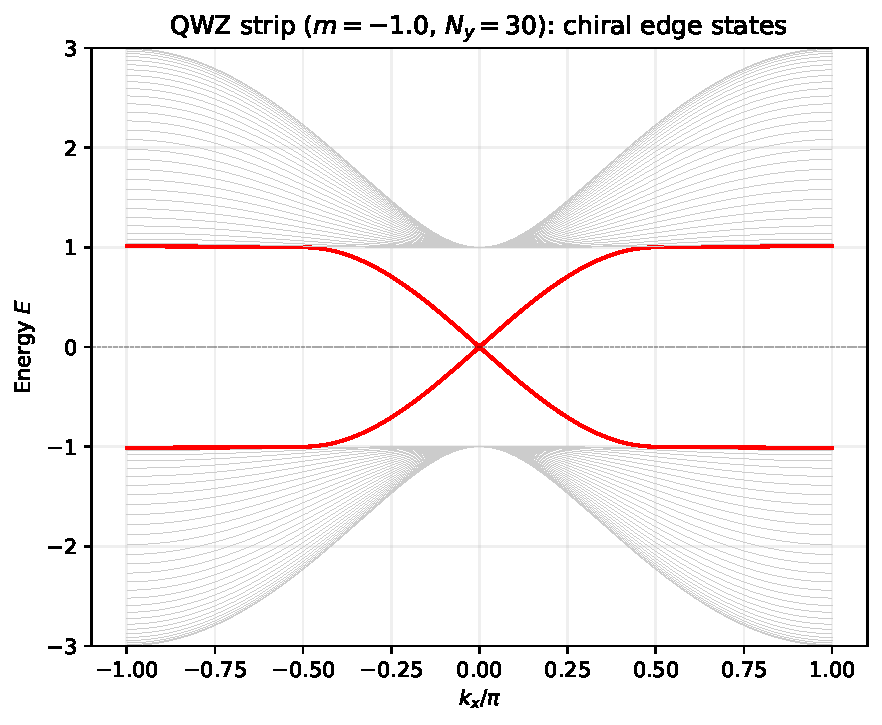
\includegraphics[width=0.6\linewidth]{figures/fig_f11_chiral_edge.pdf}
 \caption{Computed band structure of a QWZ strip ($m = -1$, $N_y = 30$).
 The 60 bulk bands (grey) form a gapped spectrum with Chern number
 $\Chern = 1$. The red branches are edge-localized modes on the two
 opposite strip boundaries; each boundary supports one chiral channel,
 with opposite group velocities on opposite edges. The branches connect
 the lower and upper bulk bands across the gap, illustrating the
 bulk--boundary correspondence.}
 \label{fig:chiral-edge-strip}
\end{figure}

\paragraph{Experimental observation.}
The photonic anomalous Hall effect was first demonstrated experimentally
by Wang et al.\ (2009) using a two-dimensional photonic crystal of YIG
rods at microwave frequencies. The experiment confirmed three
predictions of the topological theory:
\begin{enumerate}
 \item One-way edge propagation with suppressed backscattering even
 around sharp $90^\circ$ bends and metallic obstacles.
 \item The number of edge modes matches the predicted Chern number
 difference across the interface.
 \item Reversal of the external magnetic field reverses the
 propagation direction, confirming the topological origin.
\end{enumerate}
The key quantitative figure of merit is the ratio of forward to backward
transmission: in the experiment, this exceeded $50\;\mathrm{dB}$ across
the topological gap, comparable to commercial microwave isolators but
achieved without any Faraday-rotation element.

\subsection{Limitations}
\label{ssec:chern-limitations}

The magneto-optical approach has practical limitations:
\begin{itemize}
 \item The gyromagnetic effect is weak at optical frequencies, so
 large Chern gaps require strong magnetic fields or resonant
 enhancement.
 \item The materials are typically lossy, introducing non-Hermiticity
 that complicates the topological classification.
 \item The platform is most practical at microwave and millimeter-wave
 frequencies, where ferrites have large gyromagnetic responses.
\end{itemize}
Alternative approaches---Floquet modulation, coupled-ring lattices, and
synthetic gauge fields---can produce effective Chern insulators at
optical frequencies without magnetic materials.

\paragraph{Floquet photonic Chern insulators.}
An alternative route to nonzero Chern numbers at optical frequencies uses
time-periodic modulation of the refractive index~\cite{rechtsman2013photonic,ozawa2018topological}. The central idea is
that a periodically driven system has a \emph{Floquet Hamiltonian}
$H_F$ whose eigenvalues are quasi-energies $\varepsilon_n$ defined
modulo the driving frequency $\Omega$. Even if the instantaneous
Hamiltonian preserves time-reversal symmetry at every instant, the
stroboscopic evolution operator $U(T) = \mathcal{T}\exp(-i\int_0^T
H(t)\,\dd t)$ can break effective time-reversal symmetry, opening
topological gaps with nonzero Chern numbers.

The simplest photonic implementation uses a two-dimensional lattice
of coupled waveguides or ring resonators with periodically modulated
link phases. The paraxial propagation equation along the waveguide
axis $z$ plays the role of the Schr\"odinger equation:
\begin{equation}
 i\partial_z \psi(x,y,z) = H(z)\,\psi(x,y,z),
 \label{eq:paraxial-floquet}
\end{equation}
where $z$ replaces time and the lattice potential $H(z)$ is periodic
with period $Z$ (the helix pitch or modulation period). The Floquet
operator $U(Z) = \mathcal{T}\exp(-i\int_0^Z H(z')\,\dd z')$ defines
the effective Hamiltonian $H_F = (i/Z)\ln U(Z)$, and its Bloch bands
carry well-defined Chern numbers computed from the Berry curvature of
the Floquet eigenstates.

In coupled-ring-resonator lattices~\cite{hafezi2013imaging}, the link phases between
rings are engineered to simulate an effective magnetic vector potential
$\mathbf{A}_{\mathrm{eff}}$, producing Floquet bands with nonzero
Chern numbers. The key advantage is that no magnetic material is
required: time-reversal symmetry is broken by the modulation itself.
Chiral edge states have been observed experimentally in
silicon-photonic ring-resonator networks at telecom wavelengths,
demonstrating topological protection at optical frequencies with
forward-to-backward transmission contrast exceeding $10\;\mathrm{dB}$.

\paragraph{Non-Hermitian complications in Floquet systems.}
The main limitation of Floquet topological photonics is that
driven systems are inherently open: they exchange energy with the
driving field and with the environment. Material loss, radiation
leakage, and gain saturation all make the effective Floquet Hamiltonian
non-Hermitian. The quasi-energy bands become complex, and the Chern
number must be replaced by its biorthogonal generalization
(Chapter~\ref{ch:complex-bands}). Furthermore, Floquet systems can
exhibit parametric instability when the driving frequency is resonant
with inter-band transitions, leading to exponential growth of certain
modes---a Floquet-specific mechanism of non-Hermiticity that has no
static analogue. These complications connect the Floquet approach
directly to the non-Hermitian Berry connection of
Section~\ref{sec:nh-berry-preview} and the open problems of
Chapter~\ref{ch:open-problems}.


%% ================================================================
\section{Wilson loop and $\mathbb{Z}_2$ invariants}
\label{sec:wilson-loop}

For systems with time-reversal symmetry where the Chern number vanishes,
topological information is encoded in the \emph{Wilson loop}
operator~\cite{paz2019tutorial}:
\begin{equation}
 W(\ell) = \mathcal{P}\exp\!\left[-i\oint_\ell
 \mathbf{A}(\kk)\cdot\dd\kk\right],
 \label{eq:wilson-loop}
\end{equation}
where $\mathbf{A}$ is the non-Abelian Berry connection matrix for a group
of $N$ bands, $(\mathbf{A})_{mn} = i\langle\mathbf{u}_{m\kk}|\nabla_\kk|\mathbf{u}_{n\kk}\rangle_\varepsilon$,
and $\mathcal{P}$ denotes path ordering.

The eigenvalues of $W(\ell)$---the Wannier center flow---reveal the
topological phase:
\begin{itemize}
 \item \textbf{Trivial phase:} Wannier centers are constant (do not
 wind) as a function of the free momentum parameter.
 \item \textbf{$\mathbb{Z}_2$ topological phase:} Wannier centers wind
 by $\pm 2\pi$ across the Brillouin zone, corresponding to
 delocalized Wannier functions.
 \item \textbf{Obstructed atomic limit:} Wannier centers are pinned at
 non-trivial positions but do not wind.
 \item \textbf{Fragile topology:} Wannier centers wind with opposite
 slopes, and the topology can be unwound by adding trivial bands.
\end{itemize}


%% ================================================================
\section{Numerical computation}
\label{sec:berry-numerical}

\subsection{Discretized Berry curvature}
\label{ssec:discretized}

On a discrete grid of $\kk$-points in the Brillouin zone, the Berry
curvature is computed from the gauge-invariant lattice formula of
Fukui, Hatsugai, and Suzuki (FHS):
\begin{equation}
 \Fcal_n(\kk) \approx -\Im\ln\!\bigl[
 U_1(\kk)\,U_2(\kk+\delta k_1\hat{e}_1)\,
 U_1^*(\kk+\delta k_2\hat{e}_2)\,U_2^*(\kk)
 \bigr],
 \label{eq:fhs}
\end{equation}
where
\begin{equation}
 U_\alpha(\kk)=
 \frac{\langle\mathbf{u}_{n\kk}|
 \mathbf{u}_{n,\kk+\delta k_\alpha\hat{e}_\alpha}\rangle_\varepsilon}
 {|\langle\mathbf{u}_{n\kk}|
 \mathbf{u}_{n,\kk+\delta k_\alpha\hat{e}_\alpha}\rangle_\varepsilon|}
 \label{eq:fhs-link}
\end{equation}
is the phase-only link variable between adjacent $\kk$-points in
direction $\alpha$.
This formula is manifestly gauge-invariant and numerically robust: it
does not require a smooth global gauge choice~\cite{paz2019tutorial}.

\begin{figure}[t]
 \centering
 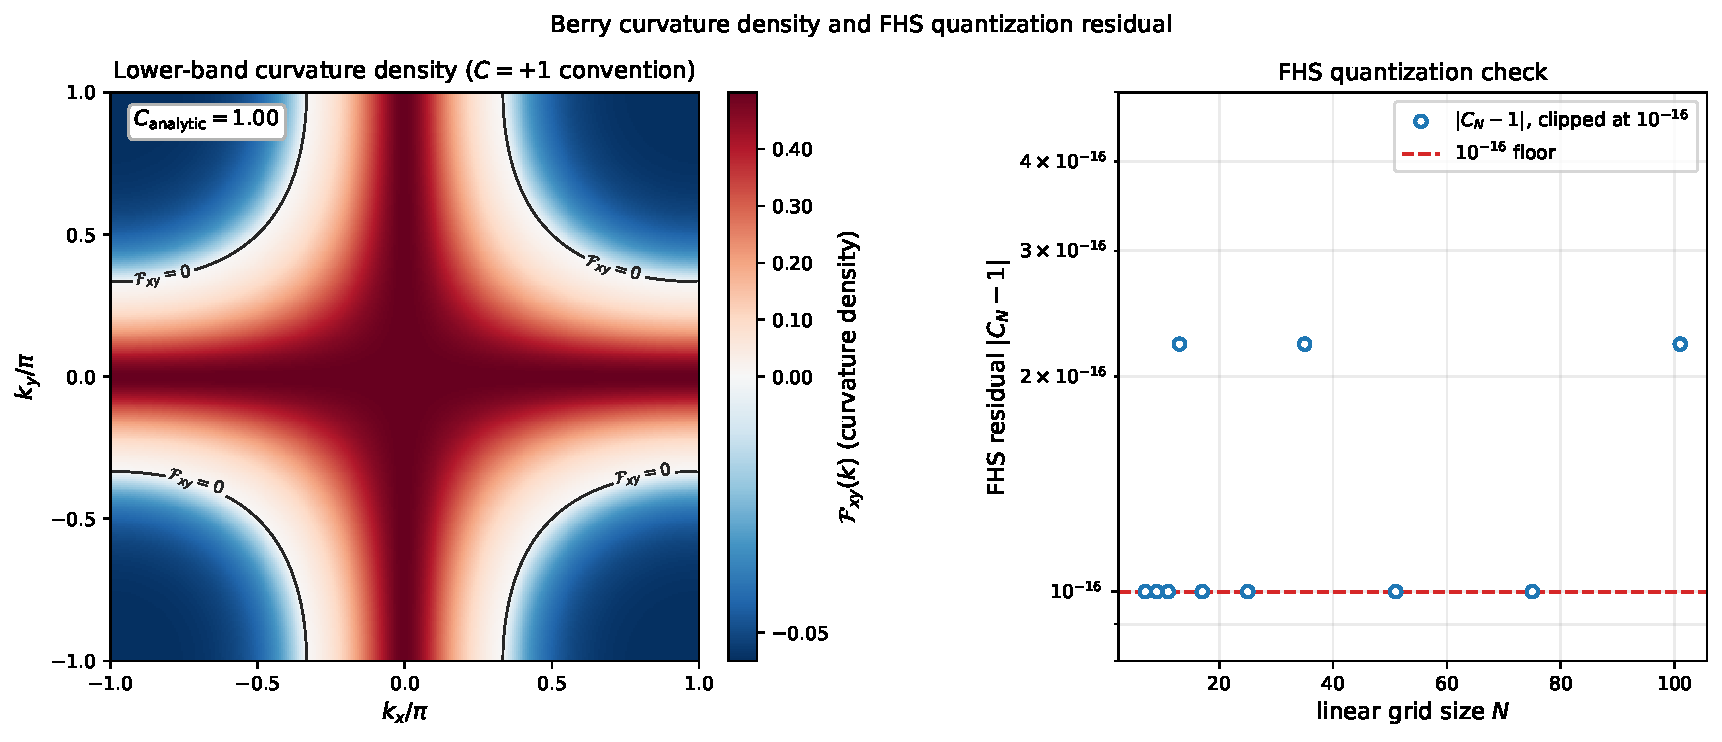
\includegraphics[width=0.95\textwidth]{fig_f11_berry_curvature_chern.pdf}
 \caption{Gauge-invariant Berry-curvature computation with the FHS link-variable algorithm. The plotted model is a two-band lattice Dirac model used as a pedagogical proxy for Maxwell Bloch bands: in a photonic calculation, the spinor overlaps are replaced by energy-inner-product overlaps of Maxwell modes. The left panel shows the analytic Berry-curvature density $\mathcal{F}_{xy}(\kk)$ for the QWZ model at $m=-1$, using the sign convention whose Brillouin-zone integral gives $C=1$. The right panel shows the FHS quantization residual $|C_N-1|$ for selected $N\times N$ grids, demonstrating machine-precision integer quantization.}
 \label{fig:berry-curvature-chern}
\end{figure}

\subsection{Practical considerations}
\label{ssec:numerical-practical}

Several practical issues arise when computing the photonic Berry
curvature numerically:
\begin{enumerate}
 \item \textbf{Band labeling:} at near-degenerate $\kk$-points, the
 eigensolver may swap band labels. The link-variable approach
 mitigates this because the overlap $U_\alpha$ automatically tracks
 the smooth band, but the grid spacing $\delta k$ must be small
 enough that the overlap is close to unity.
 \item \textbf{Grid resolution:} the Berry curvature is typically
 peaked near degeneracies and high-symmetry points. An adaptive
 grid or a finer mesh near these features improves accuracy without
 excessive computational cost.
 \item \textbf{Multi-band Chern number:} when two or more bands are
 separated from others by a common gap, the total Chern number of
 the group is computed from the non-Abelian Berry curvature
 $\Fcal_{mn}$ using
 $\Chern = (2\pi)^{-1}\int_{\BZ}\tr\Fcal\;\dd^2 k$.
 \item \textbf{Gauge smoothing:} for Wilson-loop calculations, a
 smooth gauge across one direction of the BZ is needed. The
 standard method is to fix the gauge on a reference line and
 parallel-transport it across the BZ using the SVD of the overlap
 matrix.
\end{enumerate}

\subsection{Chern number from integration}
\label{ssec:chern-numerical}

For the FHS formula, $\Fcal_n(\kk)$ is already the Berry flux through a
plaquette, so the Chern number is
\begin{equation}
 \Chern_n = \frac{1}{2\pi}\sum_{\text{plaquettes}}\Fcal_n(\kk).
 \label{eq:fhs-chern-sum}
\end{equation}
No additional factor of $\Delta k_x\,\Delta k_y$ is included. The result
is automatically an integer up to numerical precision because the
lattice formula captures the correct topology.


%% ================================================================
\section{Bulk-boundary correspondence}
\label{sec:bbc-hermitian}

The most striking physical consequence of a nonzero Chern number is the
existence of topologically protected edge states. The
\emph{bulk-boundary correspondence} states that the number of chiral edge
modes at an interface between two insulators is equal to the difference of
their gap Chern numbers:
\begin{equation}
 N_{\mathrm{edge}} = \Chern_{\mathrm{gap}}^{(\mathrm{left})}
 - \Chern_{\mathrm{gap}}^{(\mathrm{right})}.
 \label{eq:bbc}
\end{equation}
These edge states propagate in one direction only and are robust against
backscattering from disorder or defects: their existence is guaranteed by
topology, not by fine-tuned material parameters.

\subsection{Edge dispersion}
\label{ssec:edge-dispersion}

The chiral edge states have a dispersion relation $\omega(k_\parallel)$
that crosses the bulk gap. The group velocity $v_g = \dd\omega/\dd
k_\parallel$ has a definite sign (positive or negative) determined by the
Chern number. The edge modes connect the bulk bands above and below the
gap, interpolating smoothly between the valence and conduction bands.
The number of crossings equals $|\Chern|$, providing a graphical check
of the bulk-boundary correspondence.

\subsection{Robustness}
\label{ssec:edge-robustness}

In photonic Chern insulators (realized with magneto-optical materials),
the chiral edge states provide one-way waveguides for light---immune to
backscattering from fabrication imperfections, sharp bends, or surface
roughness. The robustness has a simple topological explanation: a
backscattered wave would need to reverse its direction, which requires
coupling to a counter-propagating edge mode. But only one direction of
propagation is available at each edge (there is no counter-propagating
channel), so backscattering is forbidden by topology.

This topological protection is exact in the limit of an infinite bulk
gap and degrades gradually as the gap closes. In practice, the
backscattering suppression is exponential in the ratio of the gap width
to the defect strength.

\begin{takeaway}[Hermitian bulk-boundary correspondence]
In Hermitian photonic crystals, the Chern number computed from the
Maxwell Bloch states determines the number of topologically protected
one-way edge channels. This correspondence is exact and robust: it
survives disorder, deformation, and any perturbation that does not close
the bulk gap. In non-Hermitian systems, this correspondence can fail;
the skin effect and non-Bloch bulk-boundary correspondence are the
subject of Chapters~\ref{ch:skin-effect} and~\ref{ch:bbc-rebuilt}.
\end{takeaway}


%% ================================================================
\section{Preview: non-Hermitian modifications}
\label{sec:nh-berry-preview}

The Berry curvature and Chern number derived above assumed a Hermitian
inner product and real eigenfrequencies. When non-Hermiticity is
introduced:
\begin{enumerate}
 \item The eigenfrequencies $\omega_n(\kk)$ become complex, and ``band
 gaps'' must be redefined in the complex frequency plane
 (Chapter~\ref{ch:complex-bands}).
 \item The left and right eigenvectors differ, and the Berry
 connection must be generalized to a \emph{biorthogonal} form:
 \begin{equation}
 \Acal_n^{\mathrm{bi}} = i\,
 \frac{\langle\mathbf{u}_n^{\mathrm{L}}|\nabla_\kk|\mathbf{u}_n^{\mathrm{R}}\rangle}
 {\langle\mathbf{u}_n^{\mathrm{L}}|\mathbf{u}_n^{\mathrm{R}}\rangle}.
 \label{eq:biorthogonal-berry-preview}
 \end{equation}
 The appropriate bilinear pairing depends on the Maxwell formulation
 and material dispersion; the key point is that the left mode supplies
 the dual vector. The biorthogonal Berry connection is generally
 complex-valued, and its imaginary part tracks changes in the
 left--right normalization rather than an ordinary geometric phase.
 \item New topological invariants---spectral winding numbers and
 point-gap invariants---appear that have no Hermitian analogue
 (Chapter~\ref{ch:point-gap}).
 \item The bulk-boundary correspondence can fail: the bulk Chern number
 may predict edge states that are absent, or miss states that are
 present, due to the non-Hermitian skin effect
 (Chapter~\ref{ch:skin-effect}).
\end{enumerate}

Part~IV of this book develops each of these modifications, building on
the Hermitian topological foundation established in this chapter.

\subsection{From Hermitian to biorthogonal: what changes physically}
\label{ssec:biorthogonal-physical}

The transition from Hermitian to non-Hermitian Berry curvature is not
merely a mathematical generalization; it changes the physical content
of the topological invariants.

In the Hermitian case, the Berry curvature~\eqref{eq:berry-curvature-2d}
is real-valued and determines the transverse deflection of wave packets
via~\eqref{eq:anomalous-velocity}. The Chern number counts chiral edge
modes. Both are observable through intensity measurements.

In the non-Hermitian case, the biorthogonal Berry
connection~\eqref{eq:biorthogonal-berry-preview} is generically
complex. Its real part generalizes the Hermitian Berry phase and can
govern geometric interference effects. Its imaginary part measures
geometric amplification or attenuation associated with changes in the
left--right normalization, and is closely tied to eigenvector
non-orthogonality. Near an exceptional point the biorthogonal eigenbasis
becomes singular, and encircling the defect produces the characteristic
half-integer vorticity discussed in later chapters.

The biorthogonal Chern number
\begin{equation}
 \Chern_n^{\mathrm{bi}} = \frac{1}{2\pi}\int_{\BZ}
 \Fcal_n^{\mathrm{bi}}(\kk)\;\dd^2 k
 \label{eq:biorthogonal-chern}
\end{equation}
remains integer-valued for an isolated band over the Brillouin-zone
torus, provided a smooth biorthogonal basis exists and no exceptional
degeneracy pierces the integration surface. When the relevant gap is a
point gap rather than a line gap, the natural invariant is instead a
spectral winding number of the complex band or Bloch Hamiltonian. That
shift from Chern edge-mode counting to point-gap winding and skin-effect
physics is one of the central themes of Part~IV.

\chapter{Complex Bands and Non-Hermitian Gaps}
\label{ch:complex-bands}

\begin{chapterlead}
In Hermitian photonic crystals, a band gap is a frequency window with no
propagating modes. In non-Hermitian crystals, eigenfrequencies are
complex, and the very notion of a ``gap'' must be rethought. Two
fundamentally different gap structures emerge---the \emph{line gap} and
the \emph{point gap}~\cite{kawabata2018symmetry,kawabata2019classification,ryu2010topological}---each supporting its own class of topological
invariants. The theory of complex photonic bands is developed by
introducing the two gap types with concrete examples, deriving the spectral
winding number from the complex band dispersion, and showing how the
biorthogonal Berry phase~\cite{yao2018edge,yokomizo2019non,kunst2018biorthogonal,icon2021exceptional,shen2017topological,gong2018topological} generalizes the Hermitian topological framework
to non-Hermitian systems.
\end{chapterlead}


%% ================================================================
\section{From real to complex band structure}
\label{sec:complex-bands-intro}

When the permittivity of a periodic photonic crystal acquires an imaginary
part---through material loss, gain, or radiation coupling---the Bloch
eigenproblem of Chapter~\ref{ch:periodicity} still admits solutions
labeled by $\kk$ (Bloch's theorem depends on translational symmetry, not
Hermiticity), but the eigenfrequencies become complex:
\begin{equation}
 \omega_n(\kk) = \omega_n'(\kk) + i\omega_n''(\kk).
 \label{eq:complex-band}
\end{equation}
The ``band structure'' is now a set of curves in the three-dimensional
space $(\kk, \Re\omega, \Im\omega)$, or equivalently a set of trajectories
in the complex $\omega$ plane as $\kk$ sweeps the Brillouin zone.

\subsection{How complex bands arise from Maxwell equations}
\label{ssec:complex-bands-maxwell}

The passage from real to complex bands can be understood directly from
the Maxwell eigenproblem. In a lossless periodic medium
($\Im\epsr = 0$), the operator
$\hat{\Theta}_\kk = \epsr^{-1}\curl(\mur^{-1}\curl\,\cdot\,)$ acting on
Bloch-periodic fields is self-adjoint in the $\epsr$-weighted inner
product. Its eigenvalues $\omega_n^2(\kk)/c^2$ are real and positive.

When $\Im\epsr \neq 0$, the operator ceases to be self-adjoint, and its
eigenvalues become complex. The imaginary part of the eigenfrequency
has a clear physical meaning from the energy balance:
\begin{equation}
 \omega_n''(\kk) \approx -\frac{\omega_n'(\kk)}{2}
 \frac{\int_{\mathrm{uc}} \Im\epsr(\rr)\,|\mathbf{u}_{n\kk}(\rr)|^2\;\dd^d r}
 {\int_{\mathrm{uc}} \Re\epsr(\rr)\,|\mathbf{u}_{n\kk}(\rr)|^2\;\dd^d r},
 \label{eq:omega-imag-perturbation}
\end{equation}
valid to first order in $\Im\epsr$. Modes concentrated in lossy regions
($\Im\epsr > 0$) acquire $\omega_n'' < 0$ (decay); modes in gain
regions ($\Im\epsr < 0$) acquire $\omega_n'' > 0$ (amplification).
Different Bloch modes at the same $\kk$ sample the gain/loss distribution
differently, so they can have imaginary parts with different signs and
magnitudes.

\subsection{Consequences of complexification}
\label{ssec:complex-consequences}

This complexification has immediate consequences:
\begin{itemize}
 \item Bands can no longer be ordered by frequency along the real axis;
 two bands may cross in $\Re\omega$ while being separated in
 $\Im\omega$, or vice versa.
 \item The concept of a ``gap'' must specify what it means for two
 complex-valued curves to be ``separated.''
 \item Exceptional points---where both eigenvalues and eigenvectors
 coalesce (Chapter~\ref{ch:exceptional-points})---can appear as
 singular points in the $(\kk, \omega)$ space.
 \item The standard bulk-boundary correspondence, which relates the
 Chern number to edge-state counts, may fail because the bulk
 invariant was defined assuming a real spectrum
 (Chapter~\ref{ch:bbc-rebuilt}).
\end{itemize}

\subsection{A concrete example: 1D gain--loss lattice}
\label{ssec:1d-example}

Consider a one-dimensional tight-binding model with alternating on-site
gain and loss:
\begin{equation}
 H(k) = \begin{pmatrix} i\gamma & t(1+e^{-ik}) \\
 t(1+e^{ik}) & -i\gamma \end{pmatrix},
 \label{eq:gain-loss-ssh}
\end{equation}
where $t$ is the hopping and $\gamma$ is the gain/loss rate. This is
an SSH model with a $\PT$-symmetric non-Hermitian perturbation. The
eigenvalues are
\begin{equation}
 \omega_\pm(k) = \pm\sqrt{4t^2\cos^2(k/2) - \gamma^2}.
 \label{eq:gl-ssh-eigenvalues}
\end{equation}
For any nonzero $\gamma$, momenta close to $k=\pi$ satisfy
$|2t\cos(k/2)|<|\gamma|$, so the square root is imaginary and the
corresponding Bloch states are in a $\PT$-broken sector. Momenta farther
from $k=\pi$ remain real when $|2t\cos(k/2)|>|\gamma|$. Thus this
balanced gain--loss dimer is useful for illustrating complex bands and
exceptional points, but it is not by itself the canonical point-gap
skin-effect model. For point-gap topology and skin effect one needs
non-reciprocal hopping, as in the Hatano--Nelson or asymmetric SSH
models discussed below~\cite{gong2018topological,shen2017topological}.

\paragraph{Perturbation theory for complex bands.}
The first-order imaginary shift~\eqref{eq:omega-imag-perturbation} can
be made concrete for this lattice. At $k = 0$ the Bloch modes of the
unperturbed SSH model are $|u_\pm\rangle = (1,\;\pm 1)^\transpose/\sqrt{2}$
with $\omega_\pm(0) = \pm 2t$. The gain--loss perturbation
$\delta H = i\gamma\,\sigma_z$ has matrix elements
\begin{equation}
 \langle u_\pm | \delta H | u_\pm \rangle = 0,
 \qquad
 \langle u_\pm | \delta H | u_\mp \rangle = \pm i\gamma.
 \label{eq:gl-ssh-perturbation}
\end{equation}
The diagonal elements vanish because $|u_+\rangle$ and $|u_-\rangle$
have equal weight on the gain and loss sites. The imaginary part of
$\omega_\pm$ is therefore \emph{zero} to first order at $k = 0$:
gain and loss cancel exactly, a consequence of $\PT$ symmetry.
The leading contribution to $\Im\omega$ comes from the off-diagonal
coupling at second order:
\begin{equation}
 \omega_\pm''(0) \approx \mp \frac{\gamma^2}{4t},
 \label{eq:gl-ssh-second-order}
\end{equation}
which shifts the real eigenfrequencies at $k=0$ to
$\omega_\pm(0)=\pm\sqrt{4t^2-\gamma^2}$. The imaginary part remains zero
there as long as $|\gamma|<2t$; imaginary splittings appear first near
the momenta where $4t^2\cos^2(k/2)=\gamma^2$.

\paragraph{Tracking the spectral loop.}
As $\gamma$ increases from $0$ to $2t$, the band structure undergoes a
sequence of qualitative changes:
\begin{enumerate}
 \item $\gamma = 0$: two real bands separated by a gap of width $2t$.
 The spectrum is a line segment on the real axis.
 \item $0 < \gamma < 2t$: exceptional points appear at
 $k=\pm 2\arccos(\gamma/2t)$, separating real-frequency arcs from
 imaginary-frequency arcs.
 \item $\gamma = 2t$: the real arcs shrink to $k=0$, and the remaining
 spectrum lies on the imaginary axis.
 \item $\gamma > 2t$: all momenta are in the broken sector and the
 spectrum is purely imaginary.
\end{enumerate}
This progression illustrates a general principle: \emph{complex bands
change topology at exceptional points}. Point-gap winding, however, is
most transparently generated by non-reciprocal hopping rather than by
balanced on-site gain and loss alone.


%% ================================================================
\section{Line gaps and point gaps}
\label{sec:gap-types}

The classification of non-Hermitian topological phases depends crucially
on the type of gap in the complex energy
plane~\cite{kawabata2019symmetry}.

\subsection{Line gap}
\label{ssec:line-gap}

A \emph{line gap} exists when the complex spectrum does not cross a
specified line in the complex plane---typically the real or imaginary
axis after shifting the reference frequency. Equivalently, the spectrum
can be separated into regions lying on different sides of that line. A
line gap along the real axis, for example, means that the spectrum avoids
the real axis; a line gap along the imaginary axis means that it avoids a
chosen vertical line in the complex-frequency plane.

Line gaps are the natural generalization of Hermitian band gaps: the
spectrum is separated into two regions by a line, and each region can
carry its own topological invariant. The topological classification of
systems with a line gap is closely related to the Hermitian
classification, with some modifications due to the enlarged symmetry
algebra.

\paragraph{Physical meaning.}
A line gap makes it possible to flatten the complex spectrum to a
Hermitian-like or anti-Hermitian-like form without crossing the reference
line. For photonic bands this is a spectral separation statement, not
necessarily a division into stable and unstable modes; the latter
interpretation applies only when the chosen line is the real-frequency
axis and the two spectral groups lie on opposite sides of it.

\subsection{Point gap}
\label{ssec:point-gap}

A \emph{point gap} exists when the complex spectrum avoids a single
point in the complex plane---typically the origin or a chosen reference
energy $E_{\mathrm{ref}}$. As $\kk$ sweeps the Brillouin zone, the
eigenvalues $\omega_n(\kk)$ trace closed loops in the complex plane that
may wind around $E_{\mathrm{ref}}$.

Point gaps are intrinsically non-Hermitian: in a Hermitian system the
spectrum is confined to the real axis and cannot wind around a point in
the complex plane. The topological invariant associated with a point gap
is the \emph{spectral winding number}.

\paragraph{Physical meaning.}
A nonzero winding number around a reference point means that the
complex band cannot be continuously deformed to a point without passing
through the reference energy. This topological obstruction has a
physical consequence: it predicts the non-Hermitian skin
effect (Chapter~\ref{ch:skin-effect}), in which all eigenstates under
open boundary conditions localize at one edge of the system.

\subsection{Relationship between the two gap types}
\label{ssec:gap-relationship}

Line gaps and point gaps are not alternative descriptions of the same
physics---they describe genuinely different topological structures. A
system can have a line gap without a point gap, a point gap without a
line gap, both, or neither. The relationship is:
\begin{itemize}
 \item A line-gapped spectrum avoids every reference point on the gap
 line, so point gaps can be defined there. These point gaps need not
 carry nonzero winding.
 \item A point gap with nonzero winding around $E_{\mathrm{ref}}$ is
 incompatible with a line gap along any line that extends through
 $E_{\mathrm{ref}}$ without intersecting the spectral loop.
 \item In one dimension, nonzero point-gap winding is tied to the skin
 effect, while line-gap invariants are the closer analogues of
 conventional topological edge-state indices.
\end{itemize}

\paragraph{Which gap does a photonic crystal have?}
The answer depends on the gain--loss distribution and the frequency
range. A purely lossy photonic crystal ($\Im\epsr > 0$ everywhere)
has all eigenfrequencies in the lower half-plane: it possesses a line
gap along the real axis but no point gap with nonzero winding (the
spectrum stays on one side of the line and cannot wind). A
$\PT$-symmetric crystal with balanced gain and loss can have
eigenfrequencies on both sides of the real axis: if the spectrum
forms a loop, a point gap with nonzero winding appears, but the line
gap is absent. The transition between these two regimes is the
$\PT$-symmetry breaking threshold (Chapter~\ref{ch:pt-symmetric}).

A practical diagnostic is the following: given the complex band
structure $\omega_n(\kk)$, plot the spectrum in the complex $\omega$
plane. If the spectrum stays on one side of a line, the system has a
line gap; if it forms a loop enclosing a point, it has a point gap.

The labels in such a diagram are therefore reference-dependent: changing
the line or point used to define the gap can change which invariant is
well defined.

\begin{booknote}[Two gaps, two topologies]
The 38-fold classification of non-Hermitian topological phases is built
by considering both gap types in combination with the symmetries of the
system. A complete classification must specify: (i) the spatial
dimension, (ii) the symmetry class, and (iii) whether a line gap, a
point gap, or both are present.
\end{booknote}


%% ================================================================
\section{Spectral winding number}
\label{sec:winding}

\subsection{Definition}
\label{ssec:winding-def}

For a one-dimensional periodic system with complex band structure
$\omega(k)$ (a single band for simplicity), the \emph{spectral winding
number} around a reference point $E_{\mathrm{ref}}$ is
\begin{equation}
 \boxed{
 \wnum = \frac{1}{2\pi i}\oint_{\BZ}
 \frac{\dd}{\dd k}\ln[\omega(k) - E_{\mathrm{ref}}]\;\dd k
 = \frac{1}{2\pi i}\oint_{\BZ}
 \frac{\omega'(k)}{\omega(k) - E_{\mathrm{ref}}}\;\dd k.
 }
 \label{eq:winding-number}
\end{equation}
This integer counts the number of times the complex band encircles
$E_{\mathrm{ref}}$ as $k$ traverses the Brillouin zone. It is a
topological invariant: it cannot change unless the band touches
$E_{\mathrm{ref}}$ (the point gap closes).

\begin{figure}[t]
 \centering
 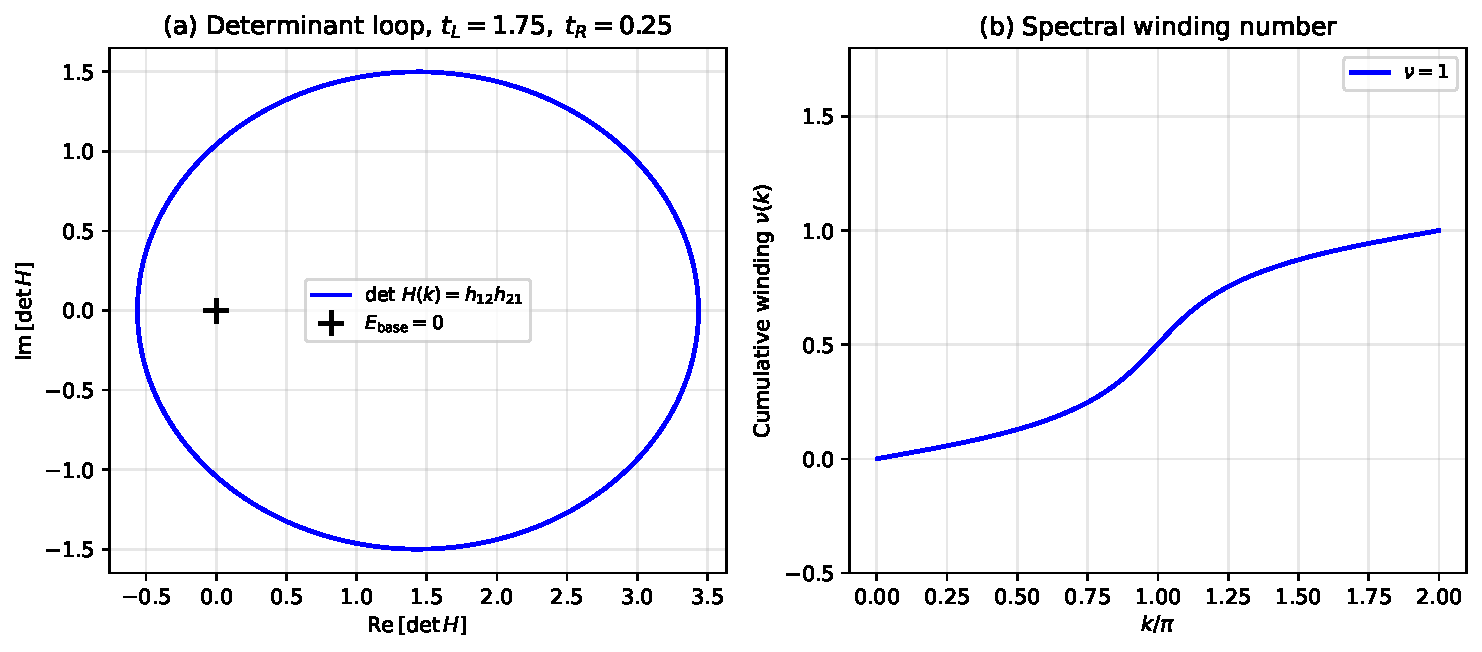
\includegraphics[width=0.85\linewidth]{figures/fig_f12_spectral_loop.pdf}
 \caption{Spectral winding number for the asymmetric-hopping NH SSH model
 ($t_L = 1.75$, $t_R = 0.25$, $t_2 = 1.0$).
 (a)~The determinant $\det H(k) = h_{12}(k)\,h_{21}(k)$ traces a loop in
 the complex plane that encircles the origin, confirming a point-gap
 topology with winding number $\nu = 1$.
 (b)~The cumulative winding accumulates smoothly from $0$ to $1$ as $k$
 traverses the Brillouin zone. Because $t_L > t_2 > t_R$, only $h_{21}$
 winds around the origin, producing a net spectral winding.}
 \label{fig:spectral-loop}
\end{figure}

\subsection{Physical meaning}
\label{ssec:winding-physical}

A nonzero winding number means the complex band forms a closed loop in
the complex $\omega$ plane that cannot be contracted to a point without
crossing $E_{\mathrm{ref}}$. This is the simplest example of a
topological invariant that exists \emph{only} in non-Hermitian systems:
a real-valued band confined to the real axis has zero winding around any
point off the axis.

In photonic crystals with complex $\epsr(\rr)$, the winding number
classifies point-gap topology of complex photonic bands. In one
dimension it is tied to the non-Hermitian skin effect under open
boundary conditions rather than to ordinary Hermitian edge-state
counting~\cite{zhong2021non}.

\subsection{Computational procedure}
\label{ssec:winding-computation}

The winding number~\eqref{eq:winding-number} is straightforward to
compute numerically:
\begin{enumerate}
 \item Sample $k$ uniformly on $[-\pi, \pi]$ with $N \gg 1$ points.
 \item Evaluate $\omega(k)$ from the Bloch eigenproblem (or from a
 tight-binding model).
 \item Form the shifted band $z(k) = \omega(k) - E_{\mathrm{ref}}$.
 \item Compute the total phase winding:
 $\wnum = [\arg z(\pi) - \arg z(-\pi)]/(2\pi)$, using the unwrapped
 phase.
 \item Alternatively, use the discrete winding formula:
 $\wnum = (2\pi)^{-1}\sum_{j=1}^{N}\arg[z(k_{j+1})/z(k_j)]$, which
 is gauge-invariant and numerically robust.
\end{enumerate}
The result is automatically an integer up to rounding errors.

\subsection{Example: Hatano--Nelson model}
\label{ssec:winding-hatano-nelson}

The Hatano--Nelson model (Chapter~\ref{ch:skin-effect}) provides a
minimal example. With asymmetric hopping $t_R \neq t_L$, the PBC band
structure is
\begin{equation}
 \omega(k) = t_R\,e^{ik} + t_L\,e^{-ik}.
 \label{eq:hn-band}
\end{equation}
This traces an ellipse in the complex plane with semi-axes
$|t_R + t_L|$ and $|t_R - t_L|$. When $t_R \neq t_L$, the ellipse has
nonzero area, and any point inside it has winding number
$\wnum = \pm 1$. Points outside the ellipse have $\wnum = 0$.

The physical consequence is striking: the OBC spectrum fills the
\emph{interior} of the PBC ellipse (see Chapter~\ref{ch:skin-effect}),
and all OBC eigenstates localize at one edge. The winding number
predicts this macroscopic spectral collapse.


%% ================================================================
\section{Biorthogonal Berry phase}
\label{sec:biorthogonal-berry}

In a non-Hermitian periodic system, the left and right Bloch eigenvectors
$\mathbf{u}_n^{\mathrm{L}}(\kk)$ and $\mathbf{u}_n^{\mathrm{R}}(\kk)$
are generally different (Section~\ref{sec:qnm-adjoint}). The Berry
connection must be generalized to a biorthogonal form:
\begin{equation}
 \Acal_n^{\mathrm{bi}}(\kk)
 = i\,\frac{\langle\mathbf{u}_n^{\mathrm{L}}(\kk)|\nabla_\kk|
 \mathbf{u}_n^{\mathrm{R}}(\kk)\rangle}
 {\langle\mathbf{u}_n^{\mathrm{L}}(\kk)|\mathbf{u}_n^{\mathrm{R}}(\kk)\rangle}.
 \label{eq:biorthogonal-berry}
\end{equation}
The biorthogonal Berry curvature and Chern number are defined analogously.
They reduce to the standard (Hermitian) definitions when the system is
Hermitian and left and right eigenvectors coincide.

\subsection{Complex-valued Berry phase}
\label{ssec:complex-berry}

Unlike the Hermitian Berry connection, which is real-valued (for a
single band), the biorthogonal Berry connection~\eqref{eq:biorthogonal-berry}
is generically complex. Its real and imaginary parts have distinct
physical meanings:
\begin{itemize}
 \item The \emph{real part} $\Re\Acal_n^{\mathrm{bi}}$ generalizes the
 Hermitian Berry connection and enters the semiclassical equations of
 motion for wave-packet dynamics.
 \item The \emph{imaginary part} $\Im\Acal_n^{\mathrm{bi}}$ is a new
 non-Hermitian contribution that describes the $\kk$-dependence of the
 mode non-orthogonality. It is related to the derivative of the
 Petermann factor with respect to $\kk$.
\end{itemize}

The Berry connection itself can be complex, but the first Chern number
of an isolated line-gapped band remains integer-valued when a smooth
biorthogonal basis exists over the Brillouin-zone torus. Exceptional
points or gap closings invalidate the construction rather than producing
a meaningful non-integer Chern number.

\paragraph{Example: biorthogonal Berry phase of the gain--loss
SSH model.}
For the gain--loss SSH model~\eqref{eq:gain-loss-ssh} with
$\gamma < 2t$ (the $\PT$-unbroken phase), the right eigenvector of the
lower band is
$|u^{\mathrm{R}}_-(k)\rangle = (1,\; -\omega_-(k)/[t(1+e^{ik})])^\transpose$
(up to normalisation). The left eigenvector is obtained by replacing
$H(k)$ with $H^\dagger(k)$. The biorthogonal Berry phase around the
Brillouin zone is
\begin{equation}
 \phi^{\mathrm{bi}} = \oint_{\BZ}
 \Acal_-^{\mathrm{bi}}(k)\;\dd k.
 \label{eq:biorthogonal-zak}
\end{equation}
For $\gamma = 0$ (Hermitian limit), this reduces to the standard Zak
phase: $\phi^{\mathrm{bi}} = \pi$ in the topological phase ($t' > t$)
and $\phi^{\mathrm{bi}} = 0$ in the trivial phase. As $\gamma$
increases, $\phi^{\mathrm{bi}}$ acquires an imaginary part that grows
continuously, but the real part remains quantized at $0$ or $\pi$ as
long as the chiral symmetry $\sigma_z H(k) \sigma_z = -H(k)$ is
preserved. At the $\PT$-breaking transition ($\gamma = 2t$), the
biorthogonal Berry phase is undefined because the denominator
$\langle u^{\mathrm{L}}_- | u^{\mathrm{R}}_- \rangle$ vanishes at the
EP.

\begin{figure}[t]
 \centering
 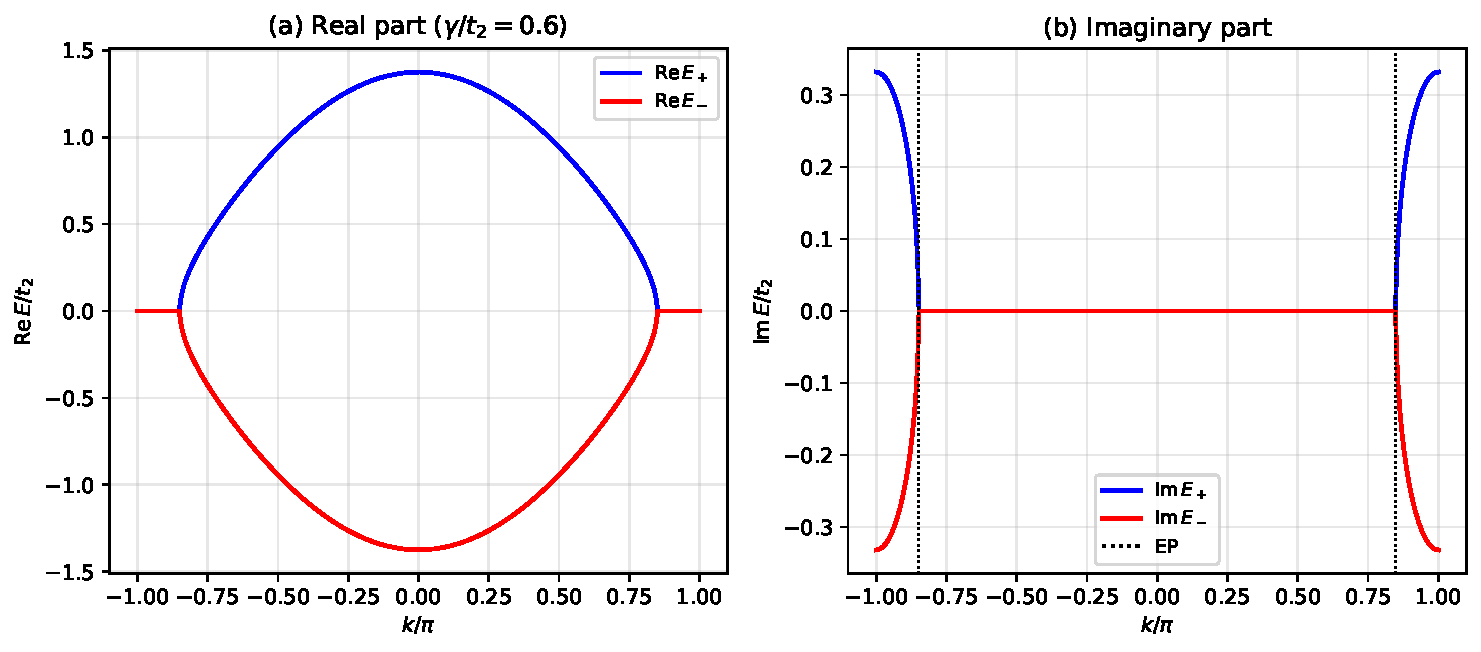
\includegraphics[width=0.85\linewidth]{figures/fig_f12_nhssh_bands.pdf}
 \caption{Complex band structure of the gain--loss SSH model
 ($t_1 = 0.5$, $t_2 = 1.0$, $\gamma/t_2 = 0.6$).
 (a)~Real part of the energy: the two bands touch near the exceptional
 points (dotted lines), where the square root in
 $E_\pm = \pm\sqrt{h_{12}h_{21} - \gamma^2}$ vanishes.
 (b)~Imaginary part: zero inside the $\PT$-symmetric region and
 bifurcating symmetrically in the $\PT$-broken region between the EPs,
 where one mode is amplified and the other is attenuated.}
 \label{fig:nhssh-complex-bands}
\end{figure}

This example illustrates a general principle: \emph{the real part of
the biorthogonal Berry phase is topologically protected by symmetry,
while the imaginary part is a smooth, non-topological measure of
non-Hermiticity.} The EP is the singularity where the Berry phase
becomes undefined---the non-Hermitian analogue of a gap closing in
Hermitian topology.

\subsection{Singularity at exceptional points}
\label{ssec:berry-ep}

Near an exceptional point, the denominator
$\langle\mathbf{u}_n^{\mathrm{L}}|\mathbf{u}_n^{\mathrm{R}}\rangle \to 0$
and the biorthogonal Berry connection diverges. This singularity reflects
the coalescence of eigenvectors and is intimately connected to the
topological charge of the EP (Section~\ref{sec:ep-topology}).

The Berry phase accumulated around a loop encircling an EP in the BZ is
$\pm\pi$ for an EP$_2$ (a $\pi$-Berry phase), analogous to the Berry
phase around a Dirac point in graphene. However, the non-Hermitian
version involves the biorthogonal inner product and does not require
time-reversal or inversion symmetry.


%% ================================================================
\section{Exceptional points in band structure}
\label{sec:ep-bands}

In a two-dimensional Brillouin zone, exceptional points appear as
isolated points in $\kk$-space where two complex bands touch. Near an
EP at $\kk_{\mathrm{EP}}$, the eigenvalue splitting follows the
square-root topology:
\begin{equation}
 \omega_\pm(\kk) \approx \omega_{\mathrm{EP}}
 \pm \sqrt{\alpha(\kk - \kk_{\mathrm{EP}})},
 \label{eq:ep-band-splitting}
\end{equation}
with $\alpha$ a complex coefficient. Encircling the EP in momentum space
exchanges the two bands---the same Riemann-surface structure as in
parameter-space encircling (Section~\ref{sec:encircling}).

\subsection{Exceptional lines and surfaces}
\label{ssec:ep-lines}

In three-dimensional systems or in systems with additional parameters,
EPs can form lines or surfaces in the combined $(\kk, \text{parameter})$
space. An \emph{exceptional ring} in a 2D BZ is a closed curve of EPs;
the interior of the ring and the exterior have different topological
indices.

In three-dimensional photonic crystals~\cite{chen2021ideal,pan2023real,liu2021observation}, exceptional points generically
form one-dimensional curves in the 3D BZ---\emph{exceptional lines}.
These lines are topological objects: they carry a topological charge
(a $\pi$ Berry phase for any loop encircling the line) and can be linked
or knotted with one another. The linking number is a topological
invariant that cannot change without two exceptional lines crossing.

\subsection{Bulk Fermi arcs}
\label{ssec:fermi-arcs}

When two complex bands are projected onto the real-frequency axis, the
regions where they overlap in $\Re\omega$ but differ in $\Im\omega$
create \emph{bulk Fermi arcs}---open arcs in the surface Brillouin zone
that connect projections of EPs. These arcs are a non-Hermitian
analogue of the Fermi arcs in Weyl semimetals~\cite{park2022nodal}, but they exist in the
bulk spectrum rather than at a surface.

The physical consequence is that constant-frequency cuts through the
complex band structure show open contours rather than closed Fermi
surfaces. This has been observed experimentally in photonic crystals
with controlled gain and loss~\cite{he2016acoustic,zhang2021acoustic}.

\paragraph{Observing bulk Fermi arcs in photonics.}
In a photonic crystal slab with $\PT$-symmetric gain and loss, bulk
Fermi arcs manifest as anomalous isofrequency contours in the
transmission spectrum. At a frequency where two complex bands overlap
in $\Re\omega$ but split in $\Im\omega$, an incident plane wave couples
to both bands with different decay rates. The transmitted intensity
shows a characteristic double-Lorentzian lineshape whose angular
dependence traces the Fermi arc in the surface Brillouin zone. The
arc endpoints are the projections of the bulk EPs, which can be located
by finding the angles at which the double Lorentzian degenerates into a
single peak with a squared-Lorentzian profile---the spectral signature
of an EP.

This measurement protocol requires only angle-resolved transmission
spectroscopy, making it accessible with standard photonic-crystal
characterization equipment. The main experimental challenge is
achieving sufficiently uniform gain--loss distribution across the
sample to resolve the Fermi-arc topology.


%% ================================================================
\section{The 38-fold classification}
\label{sec:classification}

\subsection{From tenfold to 38-fold}
\label{ssec:tenfold-to-38}

The full classification of non-Hermitian topological
phases~\cite{kawabata2019symmetry} extends the tenfold Altland--Zirnbauer
classification of Hermitian systems to 38 symmetry classes. The
expansion arises because:
\begin{enumerate}
 \item Non-Hermiticity distinguishes transposition from complex
 conjugation, doubling the number of anti-unitary symmetry classes.
 \item Both line gaps and point gaps must be considered independently.
 \item Sublattice symmetry and pseudo-Hermiticity become independent
 symmetry classes.
\end{enumerate}

Specifically, in Hermitian systems, time-reversal symmetry ($T$) and
particle-hole symmetry ($C$) are both anti-unitary and satisfy
$T H T^{-1} = H$ and $C H C^{-1} = -H$. In non-Hermitian systems,
transposition ($T^\top$: $H^\top = H$) and complex conjugation
($T^*$: $H^* = H$) are distinct symmetries because $H \neq H^\dagger$.
Similarly, $C^\top$ and $C^*$ become independent. This doubling of
symmetry types, combined with the two gap types, yields $38$ distinct
classes.

\subsection{Photonic symmetry classes}
\label{ssec:photonic-classes}

For the photonic systems that are our primary concern, the most relevant
symmetry classes and their topological invariants can be understood
through a few paradigmatic examples.

In one dimension with a point gap, the classification is $\mathbb{Z}$,
with the winding number~\eqref{eq:winding-number} as the topological
invariant. This is the symmetry class of the Hatano--Nelson model: the
asymmetric hopping breaks Hermiticity, opens a point gap, and the
resulting nonzero winding predicts the non-Hermitian skin effect. Any
one-dimensional photonic lattice with asymmetric coupling---whether from
non-reciprocal elements, spatially varying gain and loss, or
geometry-induced asymmetry---falls into this class.

In two dimensions with a line gap and broken time-reversal symmetry, the
classification is again $\mathbb{Z}$, but the invariant is the
biorthogonal Chern number of Chapter~\ref{ch:berry-maxwell}. This
generalizes the quantum Hall class to non-Hermitian systems: a magneto-optical
photonic crystal with uniform loss has complex bands separated by a line
gap, and the Chern number computed from the biorthogonal Berry
curvature correctly predicts the number of chiral edge states, even
though the edge-state frequencies are themselves complex.

Two-dimensional systems with a point gap support a different
$\mathbb{Z}$ invariant: a two-dimensional winding number that
characterizes how the complex spectrum wraps around the reference point
as $\kk$ sweeps the Brillouin zone. This invariant predicts the
two-dimensional non-Hermitian skin effect, where bulk states localize
at corners of a finite sample rather than at edges.

Finally, one-dimensional systems with $\PT$ symmetry and a line gap are
classified by $\mathbb{Z}_2$: a quantized Zak phase that takes values
$0$ or $\pi$. This is the non-Hermitian analogue of the Su--Schrieffer--Heeger
topological insulator, and the $\mathbb{Z}_2$ invariant correctly
predicts the presence or absence of $\PT$-symmetric edge states.

\paragraph{Example: symmetry-class identification for the
gain--loss SSH model.}
The systematic procedure for identifying the symmetry class of a
concrete non-Hermitian photonic system is as follows. We illustrate
each step using the gain--loss SSH model~\eqref{eq:gain-loss-ssh},
whose Bloch Hamiltonian is
$H(k) = (t_1 + t_2 \cos k)\,\sigma_x + t_2 \sin k\,\sigma_y
+ i\gamma\,\sigma_z$.

\emph{Step 1.} Write the Bloch Hamiltonian $H(\kk)$ from the Maxwell
eigenproblem. For the gain--loss SSH model, this is the $2\times 2$
matrix above with two sublattice degrees of freedom.

\emph{Step 2.} Check for time-reversal symmetry. We need
$H(\kk) = H^*(-\kk)$. Since the hopping amplitudes $t_1$, $t_2$ are
real and $i\gamma$ is purely imaginary, we find
$H^*(-k) = (t_1 + t_2\cos k)\,\sigma_x - t_2\sin k\,\sigma_y
- i\gamma\,\sigma_z$. This equals $H(k)$ only if $\gamma = 0$, so
$T^*$ symmetry is broken by the gain--loss. However, transposition
symmetry $H(k) = H^\top(-k)$ \emph{is} present because $\sigma_x$ and
$\sigma_z$ are symmetric and $\sigma_y$ is antisymmetric, and the
$\sigma_y$ coefficient is odd in $k$. This is the non-Hermitian
generalization of time-reversal for spinless particles.

\emph{Step 3.} Check for $\PT$ symmetry: $\sigma_x H(k)\sigma_x = H^*(-k)$
can be verified by direct computation. The $\sigma_x$ operator
interchanges the two sublattices (gain and loss sites), while complex
conjugation reverses the sign of $i\gamma$. Thus $\PT$ symmetry is
present, corresponding to pseudo-Hermiticity $\eta H \eta^{-1} = H^\dagger$
with $\eta = \sigma_x$.

\emph{Step 4.} Check for chiral (sublattice) symmetry:
$\sigma_z H(k) \sigma_z = -H(k)$. Direct computation confirms this:
$\sigma_z \sigma_x \sigma_z = -\sigma_x$,
$\sigma_z \sigma_y \sigma_z = -\sigma_y$, and
$\sigma_z (i\gamma\sigma_z) \sigma_z = i\gamma\sigma_z$. Wait---the
last term gives $+i\gamma\sigma_z$, not $-i\gamma\sigma_z$. So
standard chiral symmetry is broken by the gain--loss. However, a
\emph{non-Hermitian} chiral symmetry $\sigma_z H(k) \sigma_z = -H^\dagger(k)$
\emph{is} present, because $H^\dagger(k)$ flips the sign of
$i\gamma\sigma_z$.

\emph{Step 5.} Cross-reference with the 38-fold table. The combination
of transposition symmetry $T^\top$ with $(T^\top)^2 = +1$, non-Hermitian
chiral symmetry, and pseudo-Hermiticity places the system in class
BDI$^\dagger$ with a point gap. The table entry for BDI$^\dagger$ in
one dimension with a point gap is $\mathbb{Z}$: the topological
invariant is the winding number, consistent with the spectral-loop
analysis of Section~\ref{ssec:1d-example}.

\subsection{Reduction to the Hermitian tenfold way}
\label{ssec:hermitian-reduction}

The 38-fold classification must reduce to the standard tenfold
Altland--Zirnbauer classification when the Hamiltonian is Hermitian.
This consistency check is instructive. When $H = H^\dagger$:
transposition symmetry $H = H^\top$ becomes equivalent to complex
conjugation $H = H^*$ (since $H^\top = H^{\dagger *} = H^*$), so the
doubling of anti-unitary symmetries collapses. The point gap becomes
trivially satisfied (the spectrum is real and generically does not pass
through any complex reference point), so point-gap invariants become
trivial. Only line-gap invariants survive, and they coincide with the
standard band-gap invariants. The $38$ classes collapse to $10$, and
the topological periodic table reduces to the familiar Kitaev table.

For the gain--loss SSH model, taking $\gamma \to 0$ restores Hermiticity.
The BDI$^\dagger$ class collapses to the Hermitian BDI class, and the
$\mathbb{Z}$ winding number reduces to the standard winding number of
the SSH model. The point-gap topology becomes trivial (the spectrum
is real and does not wind around any complex point), and only the
line-gap $\mathbb{Z}$ invariant---the Zak phase---survives. This
continuity between non-Hermitian and Hermitian classifications is
essential for physical consistency: the topological properties of a
photonic crystal with weak gain and loss must continuously deform into
those of the passive structure.

\subsection{Beyond the periodic table}
\label{ssec:beyond-table}

The 38-fold classification is a bulk classification that applies to
infinite periodic systems. Several features of real photonic structures
lie outside its scope:
\begin{itemize}
 \item Finite-size effects modify the spectrum and can change the
 topological phase.
 \item Disorder can stabilize or destroy non-Hermitian topological
 phases, depending on the symmetry class.
 \item The classification assumes a single-particle (quadratic)
 Hamiltonian; nonlinear and many-body effects require separate
 analysis (Chapter~\ref{ch:open-problems}).
 \item The Maxwell operator has additional structure (vector nature,
 gauge redundancy, frequency-dependent material response) that is
 not fully captured by the tight-binding classification. Lifting the
 38-fold table to continuous Maxwell operators is an open problem
 (Section~\ref{sec:maxwell-synthesis}).
\end{itemize}

\begin{takeaway}[Non-Hermitian topology requires new invariants]
The topological classification of Hermitian systems---Chern numbers,
$\mathbb{Z}_2$ indices, winding numbers of real bands---is insufficient
for non-Hermitian photonics. Complex bands, point gaps, spectral winding,
and biorthogonal Berry phases introduce genuinely new topological
structures. These structures predict phenomena---the skin effect,
anomalous edge states, bulk Fermi arcs---that have no Hermitian analogue.
\end{takeaway}

\chapter{Photonic Point-Gap Topology}
\label{ch:point-gap}

\begin{chapterlead}
The spectral winding number introduced in Chapter~\ref{ch:complex-bands}
counts how many times a complex band encircles a reference point. This
chapter specializes that invariant to photonic crystals with complex
permittivity, where the non-Hermiticity is rooted in the Maxwell
equations rather than in a tight-binding model. The discussion shows how reciprocity,
the vector nature of light, and the energy inner product constrain the
point-gap topology of photonic systems, derive the winding number from
a concrete one-dimensional setting, and connect the photonic winding
number to spectral flow, boundary accumulation, and the non-Bloch
bulk--boundary correspondence that have no analogue in the Hermitian
case.
\end{chapterlead}


%% ================================================================
\section{Point-gap topology from Maxwell Bloch states}
\label{sec:point-gap-maxwell}

In a one-dimensional photonic crystal with complex periodic permittivity
$\epsr(x) = \epsr(x + a)$, the Bloch eigenproblem
\begin{equation}
 -\left(\pdv{}{x} + ik\right)\frac{1}{\epsr(x)}
 \left(\pdv{}{x} + ik\right)\psi_k(x)
 = \frac{\omega(k)^2}{c^2}\,\psi_k(x)
 \label{eq:1d-bloch-complex}
\end{equation}
yields complex eigenfrequencies $\omega(k)$ for each Bloch wave vector
$k \in [-\pi/a, \pi/a]$. As $k$ sweeps the Brillouin zone, $\omega(k)$
traces a closed curve in the complex plane (closed because
$\omega(-\pi/a) = \omega(\pi/a)$ by periodicity).

If this curve does not pass through a reference point
$E_{\mathrm{ref}}$---typically chosen as zero or the center of the
spectral loop---the spectral winding number~\eqref{eq:winding-number}
is well defined and integer-valued~\cite{yao2018edge,yokomizo2019non,shen2017topological}. A nonzero winding number indicates
that the complex photonic band has a topologically nontrivial structure
that cannot be deformed to a point without closing the point gap.

\subsection{Maxwell-level origin}
\label{ssec:maxwell-origin}

The point-gap topology of the photonic band is not an artifact of a
tight-binding approximation---it is encoded directly in the Maxwell
operator. In the full Maxwell framework, the complex eigenfrequencies
arise because the operator
$\hat{\Theta}_k = -(d/dx + ik)\epsr^{-1}(d/dx + ik)$ is non-self-adjoint
when $\Im\epsr \neq 0$. The winding of the complex bands is a
spectral property of this continuous operator, not of a discretized
model.

The key Maxwell-level insight is that the \emph{shape} of the spectral
loop in the complex plane is determined by the spatial overlap between
the Bloch mode profile and the gain/loss distribution. Modes with
different $k$ sample the gain and loss regions differently, producing
different imaginary frequency shifts (Section~\ref{ssec:complex-bands-maxwell}).
The resulting $k$-dependent imaginary part creates the loop that winds
in the complex plane.

\begin{figure}[t]
 \centering
 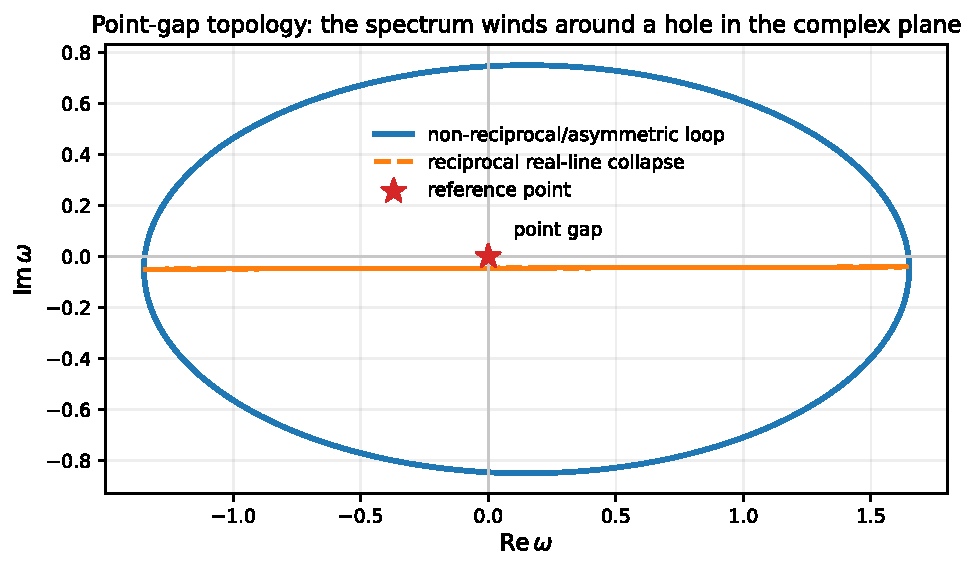
\includegraphics[width=0.72\textwidth]{fig_f13_complex_band_loop.pdf}
 \caption{A point gap is a hole in the complex spectrum, not a forbidden
 interval on the real axis. The asymmetric non-Hermitian loop winds
 around the reference point and cannot be contracted without crossing
 it; the reciprocal comparison curve collapses toward a non-winding
 real-line spectrum. The model is pedagogical, but the topology is the
 same integer winding used for complex photonic bands.}
 \label{fig:complex-band-loop}
\end{figure}

\begin{figure}[t]
 \centering
 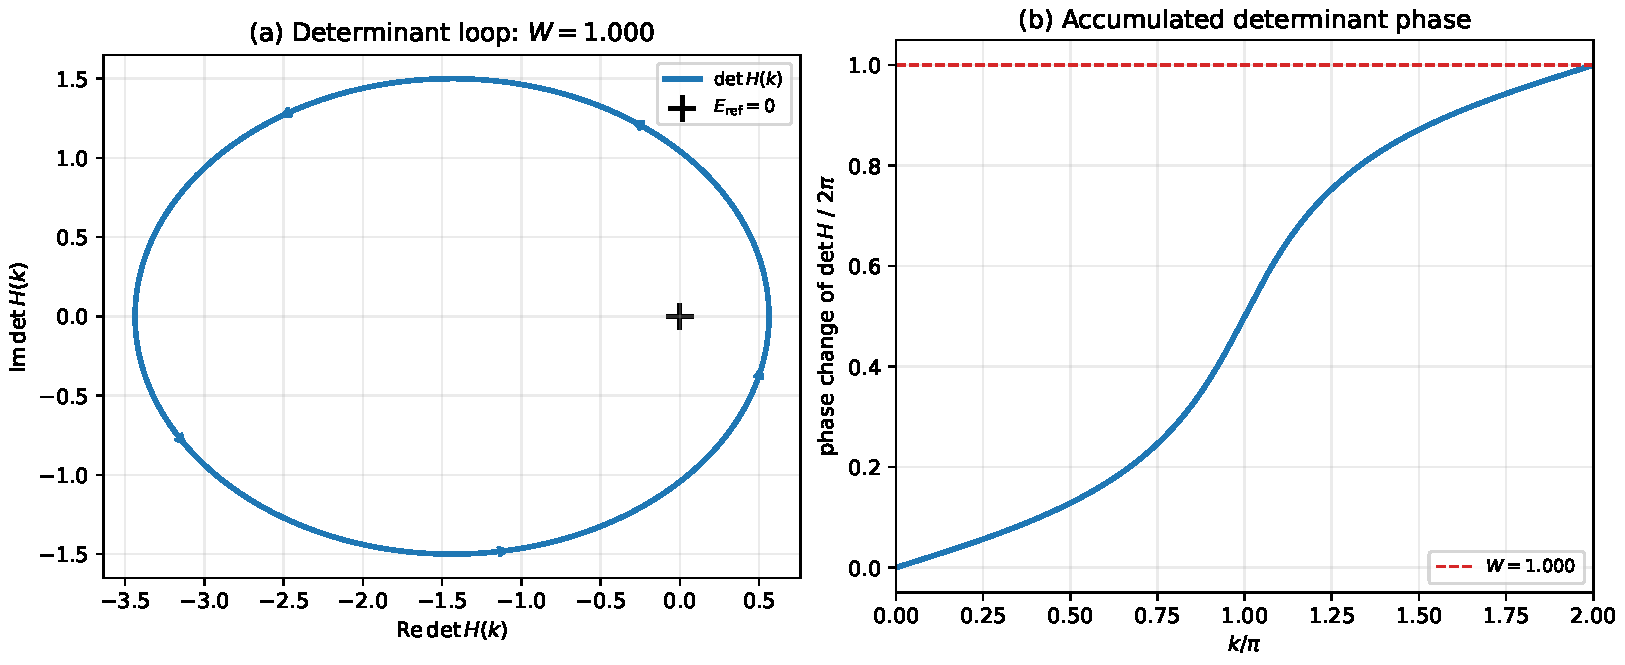
\includegraphics[width=0.85\linewidth]{figures/fig_f13_winding_number.pdf}
 \caption{Determinant winding for an asymmetric non-Hermitian SSH model
 ($t_L=1.75$, $t_R=0.25$, $t_2=1.0$). (a)~The loop traced by
 $\det H(k)$ winds once around the point-gap reference value
 $E_{\mathrm{ref}}=0$. (b)~The unwrapped phase of $\det H(k)$ changes
 by $2\pi$, giving $W=1.000000$. Computing the point-gap invariant from
 the determinant avoids branch ambiguities in square-root energy bands
 and matches the Maxwell-discretized form of the invariant.}
 \label{fig:determinant-winding}
\end{figure}

\subsection{Contrast with line-gap topology}
\label{ssec:line-vs-point}

It is instructive to contrast point-gap and line-gap topology. A
\emph{line gap} is a line in the complex plane (typically the real or
imaginary axis) that the spectrum does not cross. Line-gap topology
generalizes the Hermitian band-gap concept and supports the same
classification (Chern numbers, $\mathbb{Z}_2$ invariants) as Hermitian
systems. A \emph{point gap} is a single point that the spectrum does
not touch; the associated topology (the winding number) is purely
non-Hermitian and has no Hermitian counterpart.

For photonic systems, line-gap topology arises when the complex bands
are separated by a forbidden strip in the complex frequency plane---for
example, when gain and loss are weak enough that all bands remain close
to the real axis. Point-gap topology arises when the bands form loops
that encircle a reference energy---requiring stronger non-Hermiticity
that pushes the bands into genuinely two-dimensional curves in the
complex plane.


%% ================================================================
\section{Reciprocity constraints}
\label{sec:reciprocity-constraints}

Photonic systems are typically reciprocal (Section~\ref{sec:reciprocity}):
the permittivity tensor is symmetric, and the scattering matrix
satisfies $\Smat^\transpose = \Smat$. Reciprocity imposes a constraint
on the complex band structure: $\omega(k) = \omega(-k)$ for scalar
$\epsr$, because the Bloch Hamiltonian at $k$ and $-k$ is related by
transposition.

This constraint means the spectral loop $\omega(k)$ is symmetric under
$k \to -k$.  In one dimension, a reciprocal single-band spectral loop
necessarily retraces itself and carries zero winding, while a
multi-band determinant loop also retraces, forcing the total winding
number to vanish.  Breaking
reciprocity (e.g., with a magneto-optical component) lifts this
constraint and allows nonzero winding numbers~\cite{longhi2019probing,zhang2021observation,lin2023topological}.

\subsection{Reciprocity and vanishing point-gap winding}
\label{ssec:even-winding}

To see why reciprocity forces zero winding, write the spectral loop
as $\omega(k)$ for $k \in [-\pi/a, \pi/a]$.  Under $k \to -k$,
$\omega(-k) = \omega(k)$ (reciprocity).  The winding number
\begin{equation}
 \wnum = \frac{1}{2\pi i}\int_{-\pi/a}^{\pi/a}
 \frac{\omega'(k)}{\omega(k) - E_{\mathrm{ref}}}\;\dd k
 \label{eq:winding-integral}
\end{equation}
can be split into contributions $I_+$ (from $k \in [0,\pi/a]$) and
$I_-$ (from $k \in [-\pi/a,0]$).  Substituting $k \to -k$ in the
second integral, using $\omega(-k) = \omega(k)$ and
$\omega'(-k) = -\omega'(k)$, gives
\begin{equation}
 I_- = \frac{1}{2\pi i}\int_{0}^{\pi/a}
 \frac{-\omega'(k)}{\omega(k) - E_{\mathrm{ref}}}\;\dd k
 = -\,I_+.
 \label{eq:winding-cancellation}
\end{equation}
Therefore $\wnum = I_+ + I_- = 0$: the two half-Brillouin-zone
contributions cancel exactly.

In multi-band systems, the determinant
$\det[H(k) - E_{\mathrm{ref}}]$ also satisfies $k \to -k$ symmetry and
therefore retraces, giving zero total winding.  Individual eigenvalue
branches can still carry nonzero winding when they exchange partners at
symmetry-related $k$-points; such individual windings are constrained to
appear in cancelling pairs, so the sum vanishes.  Breaking
reciprocity---for example, with a magneto-optical
component---lifts this constraint and allows arbitrary integer
winding numbers~\cite{longhi2019probing,zhang2021observation,lin2023topological}.

\begin{booknote}[Why breaking reciprocity matters]
All one-dimensional photonic examples with nonzero point-gap winding
$\wnum \neq 0$ require broken reciprocity.  The Hatano--Nelson chain
(Chapter~\ref{ch:skin-effect}), the asymmetric SSH model, and
magneto-optical waveguide lattices all achieve $\wnum \neq 0$ precisely
because their Bloch Hamiltonians do not satisfy $H(-k)^{\mathrm{T}} = H(k)$.
In reciprocal systems, nontrivial topology protected by the transpose
symmetry can still exist, but it is classified by symmetry-protected
invariants (such as a $\mathbb{Z}_2$ index or a Pfaffian invariant)
rather than by the integer winding number $\wnum$ of the spectral
loop.  See the 38-fold classification in Chapter~\ref{ch:complex-bands}
for the full symmetry-resolved picture.
\end{booknote}

\subsection{Physical implications}
\label{ssec:even-winding-implications}

The vanishing of the ordinary reciprocal winding has concrete physical
consequences:
\begin{itemize}
 \item A reciprocal scalar 1D photonic crystal may have complex bands,
 exceptional points, or symmetry-protected non-Hermitian topology, but
 its ordinary determinant point-gap winding cancels between $k$ and
 $-k$.
 \item A nonzero integer winding in this 1D Maxwell setting normally
 requires a mechanism that makes forward and backward propagation
 inequivalent, such as magneto-optical bias, temporal modulation, or an
 engineered nonreciprocal reservoir.
 \item Breaking reciprocity (e.g., with a magneto-optical Faraday
 rotation element) allows odd winding numbers and the associated
 boundary spectral flow.
\end{itemize}

\begin{booknote}[Reciprocity and winding]
In tight-binding models, asymmetric hopping $t_L \neq t_R$ is a common
source of nonzero winding and the skin effect. In photonic crystals,
such asymmetry requires breaking reciprocity---a more demanding
experimental condition. Reciprocal photonic systems can still host
symmetry-protected non-Hermitian phases, but those phases should not be
identified with the ordinary integer winding of a single spectral loop.
The reciprocity constraint is a Maxwell-level selection rule that is
easy to miss in generic tight-binding models.
\end{booknote}


%% ================================================================
\section{Example: complex bands of a reciprocal bilayer}
\label{sec:nh-bilayer}

To make the abstract winding-number theory concrete, consider a
one-dimensional photonic crystal with period $a$ consisting of two
layers per unit cell:
\begin{itemize}
 \item Layer A: thickness $d_A = 0.5a$, index $n_A = 2.0 + 0.3i$
 (lossy).
 \item Layer B: thickness $d_B = 0.5a$, index $n_B = 2.0 - 0.1i$
 (gain, weaker than loss).
\end{itemize}
The gain and loss are \emph{not} balanced ($\PT$ symmetry is broken),
and the system is reciprocal. This example is useful because it shows
how complex photonic bands arise from Maxwell transfer matrices, but it
should not be mistaken for a nonzero point-gap winding phase: reciprocity
will make the ordinary Bloch loop retrace itself when the whole
Brillouin zone is followed.

\subsection{Transfer-matrix computation}
\label{ssec:bilayer-transfer}

The transfer matrix for one unit cell follows from the formalism of
Chapter~\ref{ch:periodicity}. Each layer contributes a propagation
matrix
\begin{equation}
 M_j = \begin{pmatrix}
 \cos\phi_j & -i\sin\phi_j/n_j \\
 -i\,n_j\sin\phi_j & \cos\phi_j
 \end{pmatrix},
 \qquad
 \phi_j = \frac{\omega\,n_j\,d_j}{c},
 \label{eq:complex-single-layer}
\end{equation}
and the full unit-cell matrix is $M = M_B\,M_A$. Because $n_j$ is now
complex, the phase $\phi_j$ has both real and imaginary parts:
$\phi_j = (\omega d_j/c)(\Re n_j + i\,\Im n_j)$. The imaginary part
causes exponential growth or decay within each layer, which is the
microscopic origin of the complex band structure.

The Bloch condition $\cos(Ka) = \xi(\omega) \equiv \tfrac{1}{2}\tr M$
generalises immediately: the half-trace $\xi$ is now complex, and the
Bloch wave vector $K$ is generically complex. For a fixed real~$k$,
the eigenfrequencies $\omega(k)$ are the solutions of
\begin{equation}
 \xi(\omega) = \cos(ka),
 \label{eq:bloch-condition-complex}
\end{equation}
which must be found numerically because the right-hand side is real
while $\xi(\omega)$ is an analytic function of $\omega$ in the complex
plane.

\paragraph{Numerical procedure.}
For each $k \in [-\pi/a, \pi/a]$, we solve
\eqref{eq:bloch-condition-complex} by Newton iteration in the complex
$\omega$ plane, initialising from the Hermitian band structure
($\Im n_j = 0$) and tracking the root as $\Im n_j$ is adiabatically
increased. With the parameters above ($n_A = 2.0 + 0.3i$,
$n_B = 2.0 - 0.1i$, $d_A = d_B = 0.5a$), the first band traces an
elliptical loop in the complex $\omega a/(2\pi c)$ plane with
centroid near $\Re\omega a/(2\pi c) \approx 0.22$ and an imaginary
spread of approximately $\pm 0.012$. The loop is tilted: the maximum
$\Im\omega$ occurs near $k = 0.3\pi/a$, not at the zone boundary,
because the mode profile at that wave vector has the largest spatial
overlap with the loss region.

The second band traces a separate loop at higher frequency. The two
loops do not intersect, confirming that the point gap between them is
well defined.

\subsection{Complex band structure}
\label{ssec:bilayer-bands}

Solving the Bloch condition numerically for $k \in [-\pi/a, \pi/a]$
yields complex eigenfrequencies $\omega(k)$. Over half of the Brillouin
zone the band can appear to form a non-circular arc in the complex
$\omega$ plane because layer A is lossier than layer B's gain. Over the
full Brillouin zone, however, the reciprocal partner at $-k$ retraces
the same spectral path. Thus the total determinant winding of this
reciprocal bilayer is zero, even though its bands are complex.

\subsection{Computing the winding number}
\label{ssec:winding-computation-ch13}

With the complex band $\omega(k)$ in hand, the spectral winding number
around a reference point $E_{\mathrm{ref}}$ is evaluated by discretising
the Brillouin zone into $N_k$ points $k_j = -\pi/a + 2\pi j/(N_k a)$
and summing the phase increments:
\begin{equation}
 \wnum = \frac{1}{2\pi}\sum_{j=0}^{N_k-1}
 \arg\!\left[
 \frac{\omega(k_{j+1}) - E_{\mathrm{ref}}}
 {\omega(k_j) - E_{\mathrm{ref}}}
 \right],
 \label{eq:discrete-winding}
\end{equation}
where $\arg$ returns a value in $(-\pi,\pi]$ and $k_{N_k} = k_0$
by periodicity. This formula is the discrete analogue
of~\eqref{eq:winding-integral}; it converges rapidly because the
spectral loop is smooth.

For the reciprocal bilayer, applying Eq.~\eqref{eq:discrete-winding} to
a single continuous band over the full Brillouin zone gives
$\wnum=0$ for any reference point not crossed by the spectrum. If one
artificially follows only half of the zone, or switches branches at a
degeneracy, an apparent winding can be obtained, but it is not the
integer point-gap invariant of the reciprocal Maxwell problem. A genuine
nonzero value requires replacing the bilayer by a nonreciprocal unit
cell so that the $k$ and $-k$ paths no longer cancel.

\begin{booknote}[Computational cost]
The bottleneck is solving~\eqref{eq:bloch-condition-complex} at each
$k_j$. For a 1D bilayer, this requires root-finding for a transcendental
equation---fast enough that the entire winding-number computation takes
milliseconds. For a 2D photonic crystal, the eigenproblem must be solved
by full-wave methods (Chapter~\ref{ch:numerics}), making the computation
substantially more expensive but still feasible with modern eigensolvers.
\end{booknote}

\subsection{Sensitivity to gain--loss contrast}
\label{ssec:bilayer-sensitivity}

As the imaginary parts of $n_A$ and $n_B$ are reduced toward zero, the
spectral loop contracts toward the real axis and eventually collapses to
a line segment (the Hermitian band structure). In the reciprocal
bilayer this contraction changes the shape of the complex band but not
the total point-gap winding, which remains zero. In a nonreciprocal
variant, by contrast, a winding transition would occur only when the
spectral path crosses the reference point and the point gap closes.

This point-gap closing is the non-Hermitian analogue of a Hermitian band
gap closing: the topological invariant can change only when the
reference point is touched by the spectrum.

Quantitatively, define a gain--loss parameter
$\gamma = \max(|\Im n_A|, |\Im n_B|)$ and fix
$\Im n_A/\Im n_B = -3$ (the ratio in our example). The critical
value $\gamma_c$ for a nonreciprocal winding transition depends on the
band gap of the underlying Hermitian structure: a larger Hermitian gap
requires a larger $\gamma_c$ to open a spectral loop wide enough to
wind. The reciprocal bilayer therefore serves as a useful warning:
large gain--loss contrast can create broad complex bands, but complex
bands alone do not imply a nonzero integer point-gap invariant.

\subsection{Relation to the Green's function}
\label{ssec:green-winding}

The point-gap winding number has an elegant reformulation in terms of
the retarded Green's function
$G(k,\omega) = [\omega^2/c^2 - \hat{\Theta}_k]^{-1}$.
At fixed reference frequency $E_{\mathrm{ref}}$, the winding can be
computed without tracking individual eigenvalues by following the phase
of the inverse Green's-function determinant across the Brillouin zone:
\begin{equation}
 \wnum(E_{\mathrm{ref}}) =
 \frac{1}{2\pi i}\int_{\mathrm{BZ}}
 \partial_k
 \ln\det\bigl[E_{\mathrm{ref}}^2/c^2 - \hat{\Theta}_k\bigr]\;\dd k,
 \label{eq:green-winding}
\end{equation}
provided the determinant never vanishes along the path. This connects
the point-gap topology directly to the analytic structure of the
photonic Green's function, which is the quantity measured in scattering
and emission experiments (Section~\ref{sec:point-gap-photonic}). In
practice, the resolvent formulation is useful for full-wave numerical
computations where the eigenfrequencies are not individually tracked but
the driven Maxwell problem can be solved at the reference frequency for
many values of $k$.


%% ================================================================
\section{From winding number to boundary response}
\label{sec:winding-to-edge}

The bulk-boundary correspondence for point-gap topology is subtler than
the Hermitian edge-state counting rule. A nonzero spectral winding of a
periodic one-dimensional system signals boundary-sensitive spectra:
under open boundary conditions the bulk eigenstates are generally
described by a generalized Brillouin zone and can accumulate near a
boundary through the non-Hermitian skin effect. The robust statement is
therefore not a simple counting formula such as
$N_{\mathrm{edge}}=|\wnum|$. Rather, the integer winding counts spectral
flow under a boundary twist and diagnoses the breakdown of the
conventional Bloch description.
This boundary response is qualitatively different from Chern edge modes
(Section~\ref{sec:bbc-hermitian}):
\begin{itemize}
 \item It can occur already in \emph{one-dimensional} systems, whereas
 Chern edge modes require at least two dimensions.
 \item It affects extensive bulk states as well as possible isolated
 defect or boundary resonances, reflecting the non-Hermitian skin
 effect (Chapter~\ref{ch:skin-effect}).
 \item It depends on the \emph{point gap}, not a line gap or a
 real-frequency band gap.
\end{itemize}

As Yao and Wang showed, the conventional Bloch-Hamiltonian winding can
give the wrong open-boundary prediction; the correct description uses
the \emph{generalized Brillouin zone} (Chapter~\ref{ch:skin-effect}).
The detailed mechanism by which the GBZ restores the bulk--boundary
correspondence is developed in Chapter~\ref{ch:bbc-rebuilt}.

\subsection{Spectral flow and parameter-driven transitions}
\label{ssec:spectral-flow}

The connection between winding number and boundary response can be
understood through spectral flow as a threading parameter is varied.
Consider a family of finite photonic systems parameterised by a twist angle
$\theta \in [0, 2\pi)$ applied as a boundary phase:
$\psi(x + La) = e^{i\theta}\psi(x)$. As $\theta$ sweeps from $0$
to $2\pi$, the finite-system eigenfrequencies trace paths in the
complex plane. The net number of eigenvalue trajectories that wind
around the reference point equals the point-gap winding $\wnum$---the
non-Hermitian analogue of the Laughlin spectral-flow argument.

This spectral flow provides an experimentally accessible probe of
point-gap topology: by threading a synthetic flux through a ring of
coupled resonators (equivalent to varying $\theta$), the movement of
resonance frequencies inside the point gap reveals the topological
invariant without computing the Bloch band structure.

\subsection{Boundary response of the bilayer}
\label{ssec:edge-bilayer}

For the reciprocal bilayer of Section~\ref{sec:nh-bilayer}, a finite
stack of $L$ unit cells with open (air) boundary conditions may support
surface resonances caused by impedance mismatch at the termination, but
these are not guaranteed by a nonzero point-gap winding because the
ordinary reciprocal winding vanishes. A nonreciprocal modification of
the same transfer-matrix model can instead produce a genuine skin
response. In that case, the bulk-mode decay length is set by the GBZ
radius deviation from unity:
\begin{equation}
 \xi_{\mathrm{skin}} \sim \frac{a}{|\ln r_{\mathrm{GBZ}}|},
 \label{eq:edge-localization}
\end{equation}
where $r_{\mathrm{GBZ}}$ is evaluated at the relevant complex
frequency. The distinction is important experimentally: observing a
localized resonance at a boundary is not by itself evidence for
point-gap topology. One must verify the boundary-sensitive spectral flow
or the non-Bloch displacement of the bulk spectrum.


%% ================================================================
\section{Two-dimensional point-gap topology}
\label{sec:2d-point-gap}

In two dimensions, point-gapped spectra have a new diagnostic absent in
one dimension: the periodic-boundary spectrum can cover a finite area in
the complex plane. The spectral-area result of Zhang, Yang, and
Fang~\cite{zhang2022universal} shows that this finite-area spectrum is
closely tied to geometry-dependent skin accumulation:
\begin{equation}
 \text{Spectral area} \neq 0
 \quad\Longrightarrow\quad
 \text{boundary-sensitive spectra in generic geometries}.
 \label{eq:spectral-area}
\end{equation}
The precise boundary response can depend on sample shape and symmetry,
so the spectral area should be read as a powerful diagnostic rather than
as a quantized invariant. It nevertheless explains why two-dimensional
non-Hermitian systems, including photonic crystal models with complex
$\epsr$, can show strong sensitivity to boundary conditions.

\subsection{Spectral area as a diagnostic}
\label{ssec:spectral-area-invariant}

For a single complex band $\omega(\kk)=x(\kk)+iy(\kk)$, a useful
oriented area with multiplicity is obtained from the Jacobian of the map
$\kk\mapsto (x,y)$:
\begin{equation}
 \mathcal{A} = \int_{\mathrm{BZ}}
 \left(\frac{\partial x}{\partial k_x}\frac{\partial y}{\partial k_y}
 - \frac{\partial x}{\partial k_y}\frac{\partial y}{\partial k_x}\right)
 \dd^2\kk
 = \int_{\mathrm{BZ}} J(\kk)\;\dd^2\kk,
 \label{eq:spectral-area-jacobian}
\end{equation}
where $J(\kk) \equiv \partial(x, y)/\partial(k_x, k_y)$ is the
Jacobian of the map $\kk \mapsto \omega(\kk)$ from the 2D Brillouin
zone to the complex energy plane. This Jacobian measures how much
oriented spectral area the band map creates locally. If $J$ has a fixed
sign, the map is orientation-preserving and the projected spectrum
covers a finite area; if $J$ changes sign, different regions of the BZ
can cancel in the oriented integral. The physical, unsigned area of the
spectral image is not generally quantized and must be interpreted with
this multiplicity caveat.

Equivalently,
\begin{equation}
 J(\kk) = 2\,\Im\!\left[
 \frac{\partial \omega_n}{\partial k_x}
 \frac{\partial \bar{\omega}_n}{\partial k_y}\right]
 = 2\left(
 \frac{\partial \Re\,\omega_n}{\partial k_x}
 \frac{\partial \Im\,\omega_n}{\partial k_y}
 - \frac{\partial \Re\,\omega_n}{\partial k_y}
 \frac{\partial \Im\,\omega_n}{\partial k_x}
 \right).
 \label{eq:jacobian-berry}
\end{equation}
This expression shows that spectral area requires the real and
imaginary parts of the eigenfrequency to vary independently across the
BZ---a hallmark of genuine non-Hermiticity, as opposed to a uniform
global loss that merely shifts all eigenvalues by a constant imaginary
offset.

\paragraph{Example: filled spectral disk.}
For a model whose two-dimensional Brillouin zone maps once onto a disk
of radius $R$ centred at $\omega_0$ in the complex plane, the unsigned
spectral area is
\begin{equation}
 \mathcal{A} = \pi R^2.
 \label{eq:circular-area}
\end{equation}
If the map covers the same disk several times with the same orientation,
the oriented area counts the multiplicity. Figure~\ref{fig:spectral-area}
illustrates the corresponding spectral image for a 2D lattice model.

This area is not a quantized topological invariant. A nonzero spectral
area instead serves as a practical diagnostic, and in generic settings a
strong indicator, of non-Hermitian boundary sensitivity in two
dimensions.

\subsection{Implications for photonic crystals}
\label{ssec:2d-photonic}

For a two-dimensional photonic crystal with complex $\epsr(\rr)$, the
PBC band structure can cover a finite area in the complex $\omega$
plane. The practical consequences are far-reaching. First, the PBC band
structure is
\emph{not} a reliable guide to the physics of a finite sample: the
eigenfrequencies of a finite photonic crystal slab can differ
qualitatively from the PBC bands, with extensive piling up of modes
near selected boundaries. Second, conventional edge or corner resonances
must be distinguished from non-Hermitian boundary accumulation using
non-Bloch theory rather than ordinary Bloch invariants. Third, the
spectral area itself can be computed efficiently from the PBC band
structure using~\eqref{eq:spectral-area-jacobian} on a discrete
$\kk$-grid, providing a practical diagnostic for boundary sensitivity in
a given 2D photonic crystal design.

\paragraph{Example: lossy square-lattice rods.}
Consider a square array of dielectric rods ($\varepsilon = 12 + 0.4i$,
radius $r = 0.2a$) in air. For TM polarization, the first band at
$\kk = (k_x, k_y)$ sweeps a closed surface in the three-dimensional
space $(\Re\omega, \Im\omega, k_x, k_y)$. Projected onto the complex
$\omega$ plane, the band covers an area
$\mathcal{A} \sim 0.003\,(2\pi c/a)^2$. Although this area is small,
it is nonzero, so the finite rod array should be checked for
boundary-sensitive spectra and possible skin accumulation. The direction
and strength of the accumulation depend on the detailed termination and
on the effective imaginary gauge field.

In practice, the skin effect in 2D photonic crystals is weaker and
harder to observe than in 1D because the spectral area scales with the
imaginary part of $\varepsilon$ and the group velocity, both of which
are modest for typical photonic-crystal parameters. Corner modes
associated with second-order point-gap topology have been predicted
theoretically but remain experimentally elusive.

\paragraph{Higher-order point-gap topology.}
In two dimensions, the point-gap classification admits a
$\mathbb{Z}$-valued second-order invariant that predicts corner-localised
modes in systems with spatial symmetries. For a photonic crystal with
$C_4$ symmetry and complex $\epsr$, the corner invariant is the
symmetry indicator or nested non-Bloch winding defined in the appropriate
generalized Brillouin zone. This higher-order topology is the
non-Hermitian analogue of the quadrupole topological insulator, but its
photonic realization requires more than gain/loss: the relevant spatial
symmetry and the non-Bloch boundary spectrum must both be verified.


%% ================================================================
\section{Photonic realizations and experiments}
\label{sec:point-gap-photonic}

Point-gap topology and the related skin response have been proposed and
observed in wave platforms including photonic analogues~\cite{he2016acoustic,yuan2025breakdown}:

\begin{figure}[t]
 \centering
 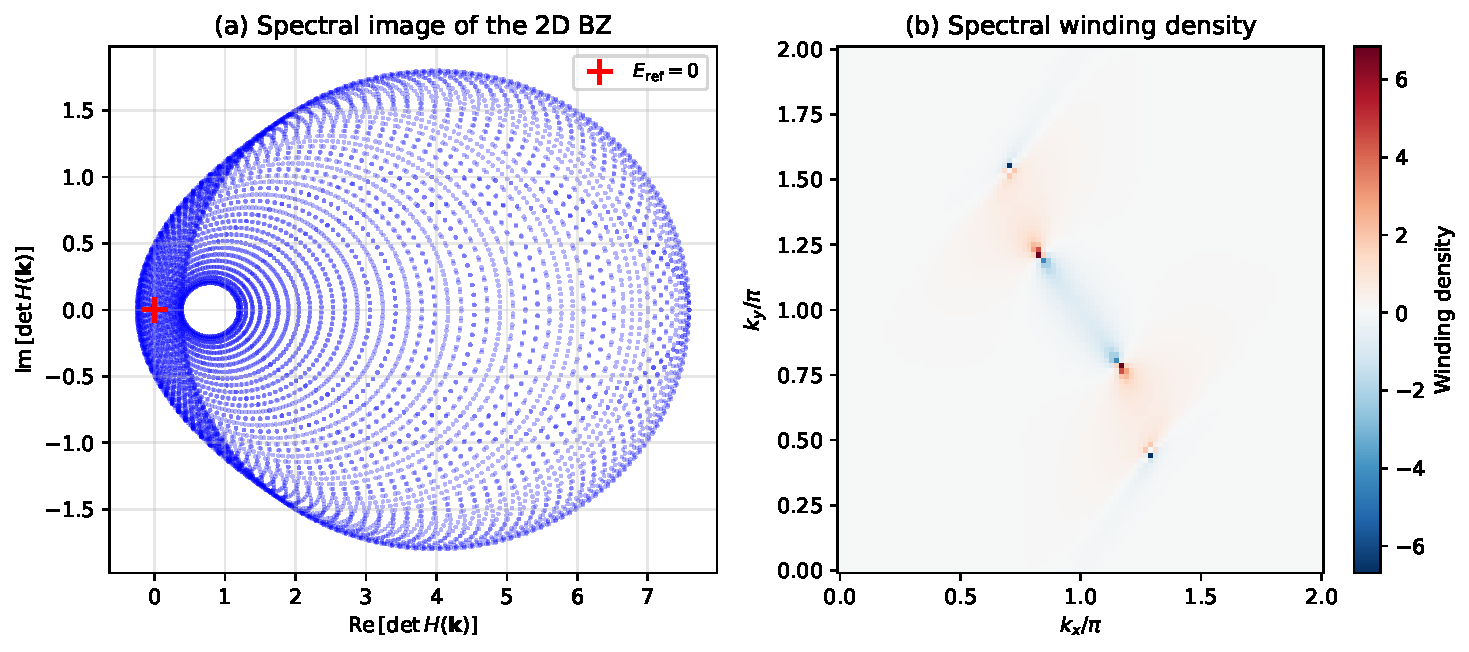
\includegraphics[width=0.85\linewidth]{figures/fig_f13_spectral_area.pdf}
 \caption{Spectral image of the 2D BZ for a non-Hermitian lattice model
 ($t_L = 1.5$, $t_R = 0.5$, $t_2 = 1.0$, $t_3 = 0.8$).
 (a)~The function $\det H(\kk)$ maps the 2D Brillouin zone into the
 complex plane (blue dots); the reference point $E_{\mathrm{ref}} = 0$
 (red cross) lies inside the image. This signals boundary sensitivity
 but is not by itself an integer edge-state count.
 (b)~Jacobian density across the BZ, showing where the map locally
 creates positive or negative oriented area. The total spectral area
 $A \approx 4.7$ is a diagnostic of non-Hermitian boundary response.}
 \label{fig:spectral-area}
\end{figure}

\paragraph{Coupled-resonator arrays.}
Chains of microring resonators with asymmetric coupling (via auxiliary
gain/loss elements) realize the non-Hermitian SSH model with tunable
winding numbers. The asymmetry can be introduced by gain/loss-induced
effective non-reciprocal coupling or by auxiliary waveguide paths that
create direction-dependent hopping. The winding number has been inferred
from the spectral sensitivity to boundary conditions and from the direct
observation of skin-mode localization.

\paragraph{Photonic lattices with on-site gain/loss.}
Arrays of waveguides with alternating gain and loss can exhibit point-gap
topology when the gain/loss pattern is combined with a mechanism that
breaks the cancellation between forward and backward propagation. In
these systems, the winding number can be tuned by varying the pump
intensity, providing a continuous knob for controlling the topological
phase.

\paragraph{Non-reciprocal photonic crystals.}
Magneto-optical photonic crystals provide a natural platform for odd
winding numbers, connecting point-gap topology to the anomalous photonic
Hall effect. These systems require an external magnetic field but offer
the largest topological gaps and the strongest skin-effect localization.

\paragraph{Photonic-crystal point-gap observation.}
Zhong et al.~\cite{zhong2021non} proposed and analyzed a concrete
photonic-crystal model with non-Hermitian point-gap topology, computing
the spectral winding number from the complex photonic band structure and
demonstrating its connection to boundary-sensitive spectra and the skin
effect. Their analysis shows that the point-gap invariant can be
extracted from full-wave electromagnetic simulations, establishing a
direct link between the abstract topological theory and realistic
photonic structures.


%% ================================================================
\section{Vector nature and polarization}
\label{sec:vector-point-gap}

In two and three dimensions, the vector nature of the electromagnetic
field introduces additional structure. Each Bloch band carries a
polarization (TE, TM, or mixed), and the point-gap winding can depend on
the polarization sector. For a 2D photonic crystal slab:
\begin{itemize}
 \item TE-like and TM-like bands can have different winding numbers,
 leading to polarization-dependent skin effects.
 \item Band crossings between TE and TM sectors can create exceptional
 points that connect the point-gap topology to the EP topology of
 Chapter~\ref{ch:exceptional-points}.
 \item The full vectorial Maxwell calculation is essential for
 quantitative predictions; scalar approximations can give the wrong
 winding number.
\end{itemize}

This polarization dependence is a uniquely photonic feature with no
analogue in scalar wave systems or electronic topological insulators.

\paragraph{Polarization-resolved winding.}
In a concrete 2D photonic crystal slab, the TE-like and TM-like bands
generally have different spatial profiles: the TM modes concentrate their
electric field inside the high-index rods, while the TE modes spread
into the air region. When $\Im\epsr$ is nonzero only inside the rods,
the TM bands acquire larger imaginary frequency shifts and trace wider
loops in the complex plane, potentially reaching a higher winding number
than the TE bands. The resulting polarisation-dependent skin effect
means that a finite photonic-crystal slab can localise TM light at one
boundary while TE light remains extended---a polarisation filter driven
entirely by non-Hermitian topology.

\paragraph{From scalar to vector: when does the winding change?}
A useful rule of thumb is that the scalar (single-polarisation)
winding number agrees with the full vectorial result whenever
the TE--TM coupling is negligible---i.e., when the photonic crystal has
a mirror symmetry that decouples the polarisations. When this symmetry
is broken (e.g., by a tilted slab, an anisotropic $\epsr$ tensor, or
a substrate), the TE and TM bands hybridise, and the winding number of
the hybridised band can differ from the sum of the individual
polarisation windings. In the extreme case of an exceptional-point
degeneracy between TE and TM bands, the winding number changes by
$\pm 1$, connecting the point-gap topology directly to the EP
classification of Chapter~\ref{ch:exceptional-points}.


\begin{takeaway}[Point-gap topology is intrinsically non-Hermitian]
Point-gap topology has no Hermitian analogue: a real-valued spectrum
cannot wind around a point in the complex plane. In photonic systems,
it arises from the interplay of complex $\epsr$, spatial periodicity,
and (optionally broken) reciprocity. The Maxwell-level constraint of
reciprocity cancels the ordinary one-dimensional determinant winding,
so genuine integer point-gap winding in photonic systems usually
requires nonreciprocity or a symmetry-resolved invariant. The physical
manifestation of point-gap topology---boundary-sensitive spectra and
the non-Hermitian skin effect---is the subject of
Chapter~\ref{ch:skin-effect}, and the rebuilt bulk-boundary
correspondence that accounts for it is developed in
Chapter~\ref{ch:bbc-rebuilt}.
\end{takeaway}

\chapter{Skin Effect and Non-Bloch Light}
\label{ch:skin-effect}

\begin{chapterlead}
In Hermitian photonic crystals, Bloch's theorem guarantees that
eigenstates are extended plane waves modulated by a periodic function.
In non-Hermitian crystals, this guarantee can fail: under open
boundary conditions, an extensive fraction of the eigenstates can pile up
at one edge of the system. This is the \emph{non-Hermitian skin effect}
(NHSE), and it demands a complete rethinking of band theory. The wave
vector acquires an imaginary part, the Brillouin zone deforms into a
\emph{generalized Brillouin zone} (GBZ), and topological invariants must
be redefined on this new contour to restore the bulk-boundary
correspondence. The theory of the skin effect is developed from the
perspective of photonic systems, leading to the non-Bloch band theory
that replaces conventional Bloch analysis.
\end{chapterlead}


%% ================================================================
\section{The breakdown of Bloch band theory}
\label{sec:bloch-breakdown}

Consider a one-dimensional non-Hermitian photonic crystal of $L$ unit
cells with open boundary conditions. In a Hermitian system, the
eigenstates of such a finite chain approach extended Bloch waves as
$L \to \infty$, with eigenfrequencies tracing the bulk bands. In a
non-Hermitian system, the picture changes.

\subsection{Skin modes}
\label{ssec:skin-modes}

Numerical diagonalization of a simple skin-effect Hamiltonian reveals
that an extensive set of eigenstates---not just a few edge states, but
the bulk spectrum itself---can become exponentially localized at one
boundary of the chain. The localization length is finite and independent
of $L$ in the standard NHSE. This is the non-Hermitian skin effect: an
$O(L)$ number of states are boundary-localized, in contrast to the
$O(1)$ boundary states of Hermitian topological insulators.

\subsection{Spectral sensitivity}
\label{ssec:spectral-sensitivity}

The open-boundary spectrum can differ strongly from the
periodic-boundary (PBC) spectrum. Under PBC, the eigenfrequencies form
closed loops in the complex plane (the bands of
Chapter~\ref{ch:complex-bands}). Under open boundary conditions (OBC),
the spectrum collapses onto arcs or curves that bear little resemblance
to the PBC loops. Conventional Bloch-Hamiltonian invariants, computed
from the PBC spectrum, fail to predict the OBC physics---including the
presence or absence of topological zero modes.

\subsection{A quantitative measure}
\label{ssec:skin-quantitative}

The skin effect can be quantified by the inverse participation ratio
(IPR) or by the mean center of mass of the eigenstates. For an $L$-site
chain with eigenstate $|\psi_j\rangle$ and amplitudes $\psi_j(n)$ at
site $n$, the center of mass is
\begin{equation}
 \bar{n}_j = \sum_{n=1}^{L} n\,|\psi_j(n)|^2
 \bigg/ \sum_{n=1}^{L} |\psi_j(n)|^2.
 \label{eq:center-of-mass}
\end{equation}
In a Hermitian system, $\bar{n}_j \approx L/2$ for bulk states. In a
standard skin-effect system, $\bar{n}_j \to 1$ (or $\bar{n}_j \to L$)
for an extensive set of eigenstates, signaling macroscopic boundary
accumulation.

\begin{figure}[t]
 \centering
 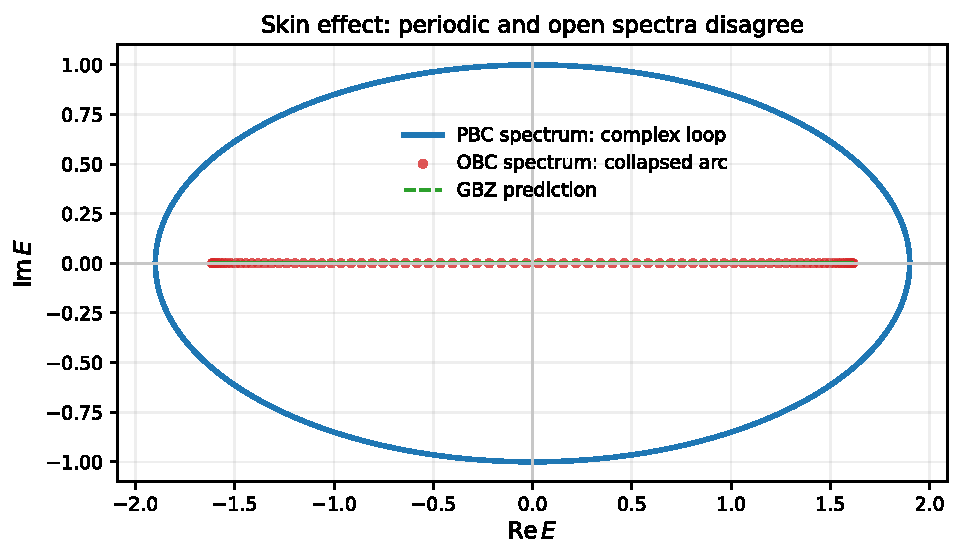
\includegraphics[width=0.72\textwidth]{fig_f14_pbc_obc_spectra.pdf}
 \caption{The non-Hermitian skin effect announces itself through spectral
 sensitivity to boundary conditions~\cite{hatano1996localization}. In the Hatano--Nelson toy model, the
 periodic-boundary spectrum forms a complex loop, while the open-boundary
 spectrum collapses onto the non-Bloch/GBZ prediction~\cite{yao2018edge,yokomizo2019non}. This is the
 computational signature behind the failure of ordinary Bloch
 bulk-boundary correspondence.}
 \label{fig:skin-pbc-obc-spectra}
\end{figure}

\begin{figure}[t]
 \centering
 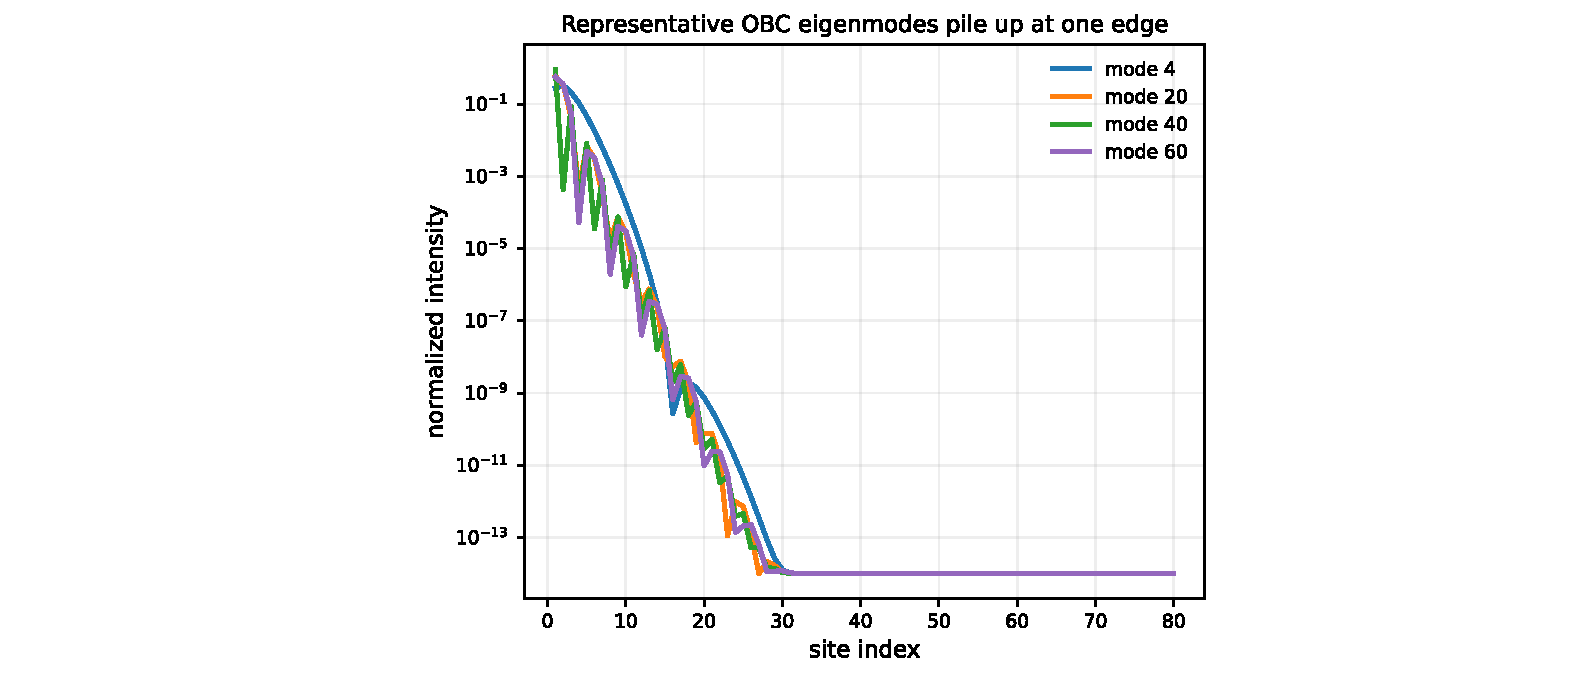
\includegraphics[width=0.95\textwidth]{fig_f14_skin_modes.pdf}
 \caption{Skin modes are not a small number of edge states; in the
 standard NHSE an extensive fraction of the open-chain eigenvectors
 accumulates near one boundary. The plotted representative normalized
 eigenmode intensities decay exponentially away from the accumulation
 edge on a logarithmic scale.}
 \label{fig:skin-mode-localization}
\end{figure}


%% ================================================================
\section{Physical origin of the skin effect}
\label{sec:skin-origin}

The skin effect arises when non-Hermiticity produces a nonzero
point-gap winding, most transparently through \emph{asymmetric} coupling
between sites. In a tight-binding picture, if the hopping amplitude from
left to right ($t_R$) differs from right to left ($t_L$), a particle is
preferentially transported in one direction, and eigenstates accumulate
at the corresponding boundary. Asymmetric hopping is the cleanest route,
but the more general diagnostic is the boundary-sensitive point-gap
spectrum discussed in Chapter~\ref{ch:point-gap}.

\subsection{Sources of asymmetry in photonic systems}
\label{ssec:asymmetry-sources}

In photonic systems, this asymmetry can arise from:
\begin{itemize}
 \item \textbf{Non-reciprocal elements:} magneto-optical materials or
 active components that break Lorentz reciprocity.
 \item \textbf{Engineered gain/loss reservoirs:} auxiliary lossy or
 amplifying paths that produce direction-dependent effective coupling
 after unobserved channels are eliminated.
 \item \textbf{Coupled-resonator networks:} auxiliary coupling paths
 that make the reduced modal hopping asymmetric. A reciprocal
 full-wave device may still have a symmetric scattering matrix; the
 nonreciprocity here is an effective description of a selected
 subsystem.
 \item \textbf{Time modulation:} periodic temporal modulation of the
 refractive index that breaks time-reversal symmetry and creates
 effective non-reciprocal hopping in the Floquet picture.
\end{itemize}

\subsection{The imaginary gauge field}
\label{ssec:imaginary-gauge}

The mathematical signature of the skin effect is that the eigenvalues
$\beta = e^{ik}$ of the transfer matrix (or the Bloch phase factor) are
no longer on the unit circle $|\beta| = 1$. Instead, they satisfy
$|\beta| = r \neq 1$, corresponding to an exponentially growing or
decaying spatial profile. The wave vector acquires an imaginary part:
$k \to k - i\kappa_{\mathrm{skin}}$, where
$\kappa_{\mathrm{skin}} = \ln r$ is the skin decay constant.

This can be understood as an \emph{imaginary gauge field}~\cite{longhi2019probing,zhang2021observation,yang2020non,yang2026non}: the
asymmetric hopping is equivalent to a uniform imaginary vector
potential. Under OBC the asymmetry can be removed from the Hatano--Nelson
Hamiltonian by a non-unitary similarity transform, but the transformed
back eigenvectors acquire an exponential envelope. Under PBC the same
transform changes the boundary condition by a complex flux, so the
asymmetry remains visible in the periodic spectrum as a complex loop.
This gauge-theoretic perspective explains why the PBC and OBC spectra
are so different.


%% ================================================================
\section{Example: the Hatano--Nelson model}
\label{sec:hatano-nelson}

The Hatano--Nelson model is the simplest system that exhibits the skin
effect. It is a one-dimensional tight-binding chain with asymmetric
nearest-neighbor hopping:
\begin{equation}
 H = \sum_{n=1}^{L-1}\bigl(t_R\,|n\rangle\langle n+1|
 + t_L\,|n+1\rangle\langle n|\bigr),
 \label{eq:hn-hamiltonian}
\end{equation}
with $t_R \neq t_L$ and $t_R, t_L > 0$.

\subsection{PBC spectrum}
\label{ssec:hn-pbc}

Under periodic boundary conditions, the Bloch Hamiltonian is
\begin{equation}
 H(k) = t_R\,e^{ik} + t_L\,e^{-ik},
 \label{eq:hn-bloch}
\end{equation}
and the eigenvalues trace an ellipse in the complex plane:
\begin{equation}
 E_{\mathrm{PBC}}(k) = (t_R + t_L)\cos k + i(t_R - t_L)\sin k,
 \label{eq:hn-pbc-spectrum}
\end{equation}
with semi-major axis $t_R + t_L$ and semi-minor axis $|t_R - t_L|$. The
spectral winding number (Section~\ref{sec:winding}) around any point
inside the ellipse is $\wnum = +1$ (for $t_R > t_L$).

\subsection{OBC spectrum}
\label{ssec:hn-obc}

Under open boundary conditions, the spectrum collapses onto the real
interval $[-2\sqrt{t_R t_L},\; 2\sqrt{t_R t_L}]$. In this model the
PBC ellipse collapses
onto a line segment. All eigenvalues are real, and all right eigenstates
localize at the left boundary (for $t_R > t_L$).  The amplitude envelope
is controlled by the GBZ radius,
\begin{equation}
  |\psi_n| \propto r_{\mathrm{GBZ}}^{\,n},\qquad
  r_{\mathrm{GBZ}}=\sqrt{\frac{t_L}{t_R}},
  \label{eq:hn-localization}
\end{equation}
so the amplitude localization length is
$\xi_{\mathrm{amp}}=1/|\ln r_{\mathrm{GBZ}}|=2/\ln(t_R/t_L)$.  If one
fits the intensity $|\psi_n|^2$ instead, the corresponding intensity
length is $\xi_{\mathrm{int}}=\xi_{\mathrm{amp}}/2=1/\ln(t_R/t_L)$.
We will state explicitly which convention is being used whenever a
localization length is quoted.

\subsection{GBZ construction}
\label{ssec:hn-gbz}

The GBZ for the Hatano--Nelson model can be found analytically. Replace
$e^{ik}$ by $\beta$ in~\eqref{eq:hn-bloch}:
$H(\beta) = t_R\beta + t_L/\beta$. The characteristic equation
$H(\beta) = E$ gives a quadratic in $\beta$:
\begin{equation}
 t_R\beta^2 - E\beta + t_L = 0,
 \label{eq:hn-characteristic}
\end{equation}
with two solutions $\beta_1, \beta_2$ satisfying
$\beta_1\beta_2 = t_L/t_R$. The GBZ condition
$|\beta_1| = |\beta_2|$ gives
\begin{equation}
 |\beta|^2 = \frac{t_L}{t_R}
 \quad\Longrightarrow\quad
 |\beta| = \sqrt{\frac{t_L}{t_R}} \equiv r_{\mathrm{GBZ}}.
 \label{eq:hn-gbz-radius}
\end{equation}
The GBZ is a circle of radius $r_{\mathrm{GBZ}} < 1$ (for $t_R > t_L$)
centered at the origin in the complex $\beta$ plane.

\begin{figure}[t]
 \centering
 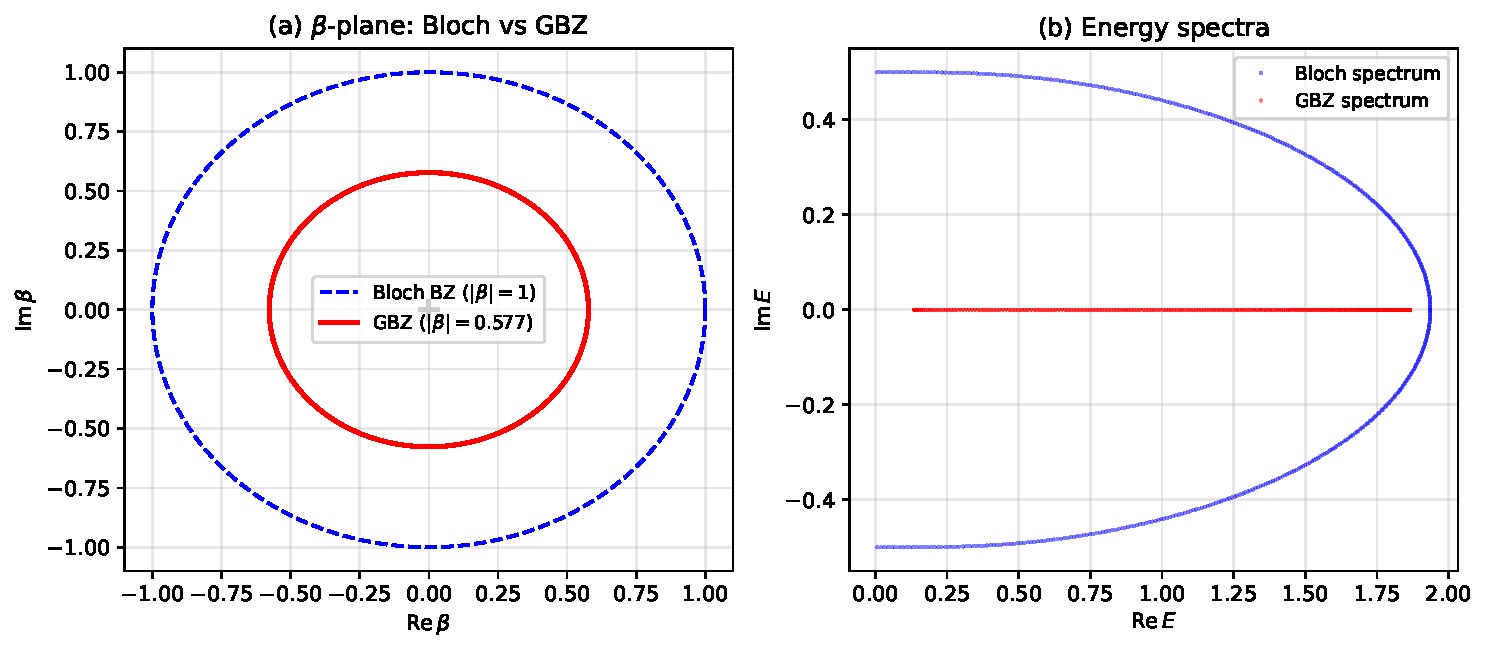
\includegraphics[width=0.85\linewidth]{figures/fig_f14_gbz_construction.pdf}
 \caption{Generalized Brillouin zone (GBZ) for an asymmetric-hopping
 Hatano--Nelson model with $t_R/t_L=3$.
 (a)~In the $\beta$-plane, the Bloch BZ (blue dashed, $|\beta| = 1$)
 and the GBZ (red solid, $|\beta| = \sqrt{t_L/t_R} \approx 0.577$)
 are concentric circles. The GBZ radius is smaller than unity,
 reflecting the exponential skin-effect localisation of all bulk
 eigenstates toward one boundary.
 (b)~The energy spectrum computed on the GBZ (red) differs
 qualitatively from the Bloch spectrum (blue), correctly reproducing
 the OBC spectrum and the non-Bloch phase boundary.}
 \label{fig:gbz-construction}
\end{figure}

Evaluating the
band structure on this circle gives
\begin{equation}
 E_{\mathrm{GBZ}}(\theta) = t_R r_{\mathrm{GBZ}}\,e^{i\theta}
 + t_L\,\frac{e^{-i\theta}}{r_{\mathrm{GBZ}}}
 = 2\sqrt{t_R t_L}\,\cos\theta,
 \label{eq:hn-gbz-bands}
\end{equation}
which is exactly the OBC spectrum. The non-Bloch band theory recovers
the correct open-boundary spectrum from the deformed Brillouin zone.

The GBZ radius also fixes the skin envelope.  For amplitudes,
\begin{equation}
  \xi_{\mathrm{amp}} = \frac{1}{|\ln r_{\mathrm{GBZ}}|}
  = \frac{2}{\ln(t_R/t_L)},
  \label{eq:hn-amplitude-length}
\end{equation}
whereas an intensity fit gives
$\xi_{\mathrm{int}}=\xi_{\mathrm{amp}}/2=1/\ln(t_R/t_L)$.  This resolves
the apparent factor-of-two ambiguity: the GBZ radius describes the field
amplitude, while many numerical and experimental plots fit intensity.

\paragraph{Worked numerical example.}
Set $t_R = 1.5$ and $t_L = 0.5$, so that $t_R/t_L = 3$. The PBC
spectrum~\eqref{eq:hn-pbc-spectrum} is an ellipse with semi-major axis
$t_R + t_L = 2.0$ and semi-minor axis $|t_R - t_L| = 1.0$. The spectral
winding number around the origin is $\wnum = +1$, predicting the skin
effect. The OBC spectrum collapses onto the real interval
$[-2\sqrt{0.75},\; 2\sqrt{0.75}] \approx [-1.732,\; 1.732]$. The GBZ
radius is $r_{\mathrm{GBZ}} = \sqrt{1/3} \approx 0.577$, giving a
skin decay constant $\kappa_{\mathrm{skin}} = |\ln r_{\mathrm{GBZ}}|
= \ln\sqrt{3} \approx 0.549$ per site.  The amplitude localization
length is therefore $\xi_{\mathrm{amp}}\approx 1.82$ sites, while an
intensity fit gives $\xi_{\mathrm{int}}\approx 0.91$ sites. For a chain
of $L = 40$ sites,
numerical diagonalisation gives a mean eigenmode centre of mass
$\bar{n} \approx 1.8$, far from the Hermitian bulk value of $20.5$;
the imaginary gauge field $A_{\mathrm{imag}} = i\kappa_{\mathrm{skin}}
\approx 0.549i$ per lattice constant captures this accumulation exactly.

This example is deliberately extreme ($t_R/t_L = 3$) to make the skin
effect visible in a short chain. In photonic realisations the asymmetry is
typically smaller ($t_R/t_L \lesssim 2$), but the localization is still
measurable over chains of 10--20 resonators.

\begin{figure}[t]
 \centering
 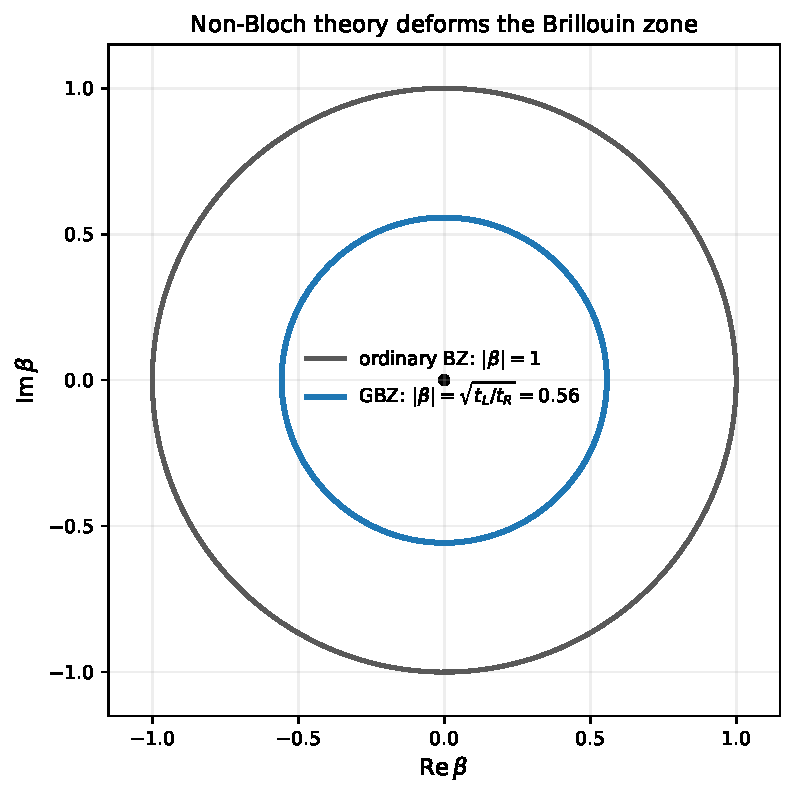
\includegraphics[width=0.58\textwidth]{fig_f14_gbz.pdf}
 \caption{The generalized Brillouin zone deforms the ordinary unit
 circle in the complex $\beta=e^{ik}$ plane. For the Hatano--Nelson
 chain with asymmetric hopping, the GBZ is the circle
 $|\beta|=\sqrt{t_L/t_R}$, which encodes the exponential envelope of
 the open-boundary eigenstates.}
 \label{fig:gbz-circle}
\end{figure}


%% ================================================================
\section{The generalized Brillouin zone: general theory}
\label{sec:gbz}

\subsection{From Bloch to non-Bloch}
\label{ssec:non-bloch}

In the conventional Bloch theory, the wave vector $k$ is real and the
Bloch phase $\beta = e^{ik}$ traces the unit circle $|\beta| = 1$ as
$k$ sweeps the BZ. The energy bands $\omega(k)$ are functions of this
real $k$.

For a non-Hermitian system with the skin effect, the correct ansatz for
the spatial dependence is $\psi_n \propto \beta^n$ with $|\beta| \neq 1$.
The appropriate contour for $\beta$ in the complex plane is the
\emph{generalized Brillouin zone} (GBZ), defined as the locus of
$\beta$ values that satisfy the bulk equation and the open-boundary
condition simultaneously.

\subsection{Construction of the GBZ}
\label{ssec:gbz-construction}

For a system with transfer matrix $\Tmat(\omega, \beta)$, the
characteristic equation
\begin{equation}
 \det[\Tmat(\omega, \beta) - \mathbf{I}] = 0
 \label{eq:characteristic}
\end{equation}
yields $2n$ solutions $\beta_1, \beta_2, \ldots, \beta_{2n}$ (for an
$n$-band model) at each complex frequency $\omega$. Ordering them by
modulus, $|\beta_1| \le |\beta_2| \le \cdots \le |\beta_{2n}|$, the GBZ
is defined by the condition
\begin{equation}
 |\beta_n| = |\beta_{n+1}|.
 \label{eq:gbz-condition}
\end{equation}
This condition ensures that the $n$-th and $(n+1)$-th solutions have
equal decay rates, which is necessary for the boundary conditions at both
ends of an open chain to be satisfied simultaneously.

\subsection{Geometry of the GBZ}
\label{ssec:gbz-geometry}

The GBZ is generically a closed curve in the complex $\beta$ plane,
but it need not be a circle. For the Hatano--Nelson model the GBZ is
the circle $|\beta| = r_{\mathrm{GBZ}}$
(Section~\ref{ssec:hn-gbz}), but richer models produce richer
contours. As the system approaches the Hermitian limit
($t_R \to t_L$), the GBZ smoothly deforms back to the unit circle,
recovering Bloch theory.

\paragraph{NH SSH model: a two-band example.}
The non-Hermitian SSH model has two sublattices per unit cell, with
the Bloch Hamiltonian
\begin{equation}
 H(\beta) = \begin{pmatrix}
 0 & t_1 + t_2/\beta \\
 t_1' + t_2'\,\beta & 0
 \end{pmatrix},
 \label{eq:nhssh-bloch}
\end{equation}
where $t_1, t_2$ are intra- and inter-cell hoppings for the
forward-going off-diagonal element and $t_1', t_2'$ for the
backward-going one. Non-Hermiticity enters whenever $t_1 \neq t_1'$
or $t_2 \neq t_2'$. The energy eigenvalues are
\begin{equation}
 E^2(\beta) = (t_1 + t_2/\beta)(t_1' + t_2'\,\beta).
 \label{eq:nhssh-energy}
\end{equation}
This is a Laurent polynomial in $\beta$; expanding gives a quartic
equation in $\beta$ at fixed $E$, yielding four roots
$\beta_1, \ldots, \beta_4$ ordered by modulus. The GBZ condition
$|\beta_2| = |\beta_3|$ (the middle pair for a two-band model) defines
the GBZ contour.

For the symmetric case $t_1 = t_1' = t$ and
$t_2 = t_2' \equiv s$ (the Hermitian SSH model), the four roots
satisfy $|\beta_1| \le |\beta_2| = |\beta_3| \le |\beta_4|$ on the
unit circle, recovering the standard BZ. But when
$t_2 \neq t_2'$---for instance $t_2 = t_2' + \delta$ with $\delta$
parameterising the asymmetry---the GBZ deforms into a non-circular
closed curve. Near the exceptional points of the band structure,
the contour develops cusps where the two middle roots collide in
both modulus and phase.

The physical content of the GBZ shape is transparent: the deviation
of $|\beta|$ from unity at each point on the GBZ measures the local
skin-mode decay rate. Regions of the GBZ where $|\beta| < 1$
correspond to modes that decay into the bulk from the left boundary;
regions where $|\beta| > 1$ decay from the right boundary. The
overall bias of the GBZ toward $|\beta| < 1$ or $|\beta| > 1$
determines the direction of the macroscopic skin effect.

\paragraph{Photonic transfer-matrix connection.}
In photonic systems, the GBZ formalism connects directly to the
transfer-matrix method of Chapter~\ref{ch:periodicity}, but an important
caveat is needed. For an ordinary reciprocal one-dimensional stack of
isotropic layers, the $2\times2$ transfer matrix written in the usual
field variables is unimodular even when the refractive indices are
complex. Gain and loss make the half-trace complex, so the Bloch
frequencies and Bloch multipliers can be complex, but this alone does
not produce the Hatano--Nelson skin effect.

The transfer-matrix eigenvalues obey
\begin{equation}
 \beta_{1,2} = \xi \pm \sqrt{\xi^2 - 1},
 \qquad \xi = \tfrac{1}{2}\operatorname{Tr}\Tmat_{\mathrm{cell}},
 \label{eq:photonic-transfer-eigenvalues}
\end{equation}
with $\beta_1\beta_2=1$ for a unimodular reciprocal cell. Inside a stop
band one solution grows while the other decays, as in ordinary evanescent
Bloch theory; this is not by itself an extensive skin effect. To obtain
a photonic GBZ analogous to the Hatano--Nelson model one needs a unit
cell whose effective evolution is non-unimodular or nonreciprocal after
projecting to the modal subspace of interest, for example through
magneto-optical bias, temporal modulation, cascaded gain/loss reservoirs,
or a multi-port network with eliminated channels.

In such an effective model the GBZ radius is determined by the middle
roots of the characteristic equation, just as in
Eq.~\eqref{eq:gbz-condition}, and the skin localisation length is
$\xi_{\mathrm{skin}}=1/|\ln r_{\mathrm{GBZ}}|$. The physical origin is
then a direction-dependent round-trip amplification that cannot be
removed without changing the boundary condition.

\paragraph{Quantitative photonic example.}
Consider an effective coupled-resonator chain engineered to have
$t_R/t_L=1.8$ at $\lambda=1550\;\mathrm{nm}$ with lattice spacing
$a=400\;\mathrm{nm}$. The Hatano--Nelson estimate gives
$r_{\mathrm{GBZ}}=\sqrt{t_L/t_R}\approx0.745$ and an amplitude
localisation length
$\xi_{\mathrm{amp}}=1/|\ln r_{\mathrm{GBZ}}|\approx3.4$ unit cells
($1.4\;\mu\mathrm{m}$). In a finite chain of $L=30$ resonators the
right eigenmodes therefore show a clearly resolvable boundary envelope.
The precise number in a full Maxwell simulation depends on radiation
loss, coupling dispersion, and how the auxiliary channels are eliminated,
but the logarithmic relation between $r_{\mathrm{GBZ}}$ and the field
envelope is the same.

\paragraph{Energy-dependent GBZ.}
An important subtlety is that the GBZ depends on the energy $E$.
At different complex energies, the condition
$|\beta_n| = |\beta_{n+1}|$ is satisfied by different $\beta$ values,
tracing out an energy-dependent contour. The \emph{physical} GBZ
relevant for the OBC spectrum is the union of these contours over the
set of OBC eigenvalues. In practice, one often computes the GBZ at a
reference energy (e.g.\ $E = 0$ for chiral-symmetric models) and uses
it to evaluate topological invariants, but this simplification can
fail when the band structure has a complicated topology in the
$(\beta, E)$ space.

\subsection{Non-Bloch band structure}
\label{ssec:non-bloch-bands}

The \emph{non-Bloch band structure} is obtained by evaluating the
eigenvalues $\omega(\beta)$ on the GBZ contour rather than on the unit
circle:
\begin{equation}
 \omega_n^{\mathrm{OBC}} = \omega_n(\beta)\big|_{\beta \in \mathrm{GBZ}}.
 \label{eq:non-bloch-bands}
\end{equation}
This non-Bloch band structure reproduces the OBC spectrum in the
thermodynamic limit, resolving the discrepancy between PBC and OBC that
signaled the breakdown of conventional Bloch theory.


%% ================================================================
\section{Non-Bloch topological invariants}
\label{sec:non-bloch-invariants}

Topological invariants must be computed on the GBZ, not the conventional
BZ, to correctly predict open-boundary spectra and any protected
boundary modes of a non-Hermitian system.

\subsection{Non-Bloch winding number}
\label{ssec:non-bloch-winding}

For a one-dimensional system with chiral symmetry, the non-Bloch winding
number is
\begin{equation}
 \wnum_{\mathrm{GBZ}} = \frac{1}{2\pi i}
 \oint_{\mathrm{GBZ}}
 \frac{\dd}{\dd\beta}\ln\det[H(\beta)]\;\dd\beta,
 \label{eq:non-bloch-winding}
\end{equation}
where $H(\beta)$ is the Bloch Hamiltonian with $e^{ik}$ replaced by
$\beta$. This invariant correctly predicts the number of topological
zero modes under OBC, in contrast to the conventional winding number
computed on the unit circle.

\subsection{Non-Bloch Chern number}
\label{ssec:non-bloch-chern}

In two dimensions, the non-Bloch Chern number is defined by integrating
the Berry curvature over the GBZ torus (the product of two GBZ contours
for $\beta_x$ and $\beta_y$). When the non-Bloch torus is well defined,
this invariant restores the bulk-boundary correspondence for
two-dimensional non-Hermitian systems with a line gap, predicting the
correct number of chiral edge modes.

\subsection{When GBZ invariants differ from Bloch invariants}
\label{ssec:gbz-vs-bloch}

The GBZ and Bloch invariants can differ whenever the GBZ is not the unit
circle---i.e., whenever the skin effect is present. The discrepancy
is maximized when:
\begin{itemize}
 \item The asymmetry $|t_R/t_L|$ is large (strong skin effect).
 \item The system is near a phase boundary where the Bloch invariant
 changes but the GBZ invariant does not, or vice versa.
 \item The GBZ geometry has cusps or self-intersections that cross
 branch cuts of the Bloch Hamiltonian.
\end{itemize}
In all cases, the GBZ invariant is the quantity that should be compared
with open-boundary spectra and boundary modes.

\begin{takeaway}[Non-Bloch band theory]
In non-Hermitian photonic systems with the skin effect, the conventional
Bloch band structure and Bloch topological invariants give incorrect
predictions for open-boundary physics. The generalized Brillouin zone
and the non-Bloch invariants computed on it restore the bulk-boundary
correspondence and provide a faithful description of the photonic
spectrum and boundary modes.
\end{takeaway}


%% ================================================================
\section{Skin effect in two and higher dimensions}
\label{sec:skin-2d}

The skin effect in higher dimensions is qualitatively richer than in
one dimension~\cite{zhang2022universal}.

\paragraph{Universality.}
In two and higher dimensions, the spectral-area result
(Section~\ref{sec:2d-point-gap}) shows why skin accumulation is generic
in many non-Hermitian models: a PBC spectrum that covers finite area in
the complex plane is highly sensitive to boundary geometry. The precise
skin pattern can depend on sample shape, symmetry, and termination, so
the finite spectral area should be viewed as a diagnostic of boundary
sensitivity rather than as a simple one-dimensional winding number.

\paragraph{Corner skin effect.}
In certain two-dimensional systems, all eigenstates are localised at
\emph{corners} rather than edges. This corner-skin effect is a
higher-order analogue of the one-dimensional skin effect and is
classified by a second-order topological invariant. Physically, it
arises when the spectral winding numbers in the $x$ and $y$ directions
are both nonzero but with the same sign, so that the combined
localisation direction points toward a corner.

\paragraph{Geometry-dependent skin effect.}
Some systems exhibit the skin effect for generic polygon-shaped samples
but not for samples with specific symmetry-related shapes. This
geometry dependence has no analogue in Hermitian physics, where the
spectrum is insensitive to the sample shape in the thermodynamic limit.
The physical origin is that the skin localisation direction is determined
by the spectral winding, which depends on the boundary orientation;
different facets of a polygon can have different winding numbers, leading
to competing localisation directions.

\paragraph{Scale-free skin effect.}
A recently discovered variant, the scale-free skin effect, features
localisation lengths that grow with the system size $L$ rather than
remaining fixed. In these systems, the spectrum is sensitive to boundary
conditions at \emph{every} scale, not just in the thermodynamic limit.
The GBZ approaches the unit circle algebraically rather than
exponentially as $L \to \infty$, leading to a non-extensive but still
macroscopic accumulation of states at the boundary.


%% ================================================================
\section{Photonic skin effect}
\label{sec:photonic-skin}

The skin effect has been proposed and observed in several photonic
platforms:

\paragraph{Coupled-resonator optical waveguides.}
Arrays of microring resonators with engineered asymmetric coupling
realise one-dimensional non-Hermitian lattices with tunable skin
effect. The asymmetry is introduced by auxiliary gain/loss elements
or by directional couplers. The key experimental signature is that
light injected at any point in the array propagates preferentially
toward one end, regardless of the injection site.

\paragraph{Photonic mesh lattices: a concrete platform.}
Fibre-loop networks provide a versatile time-multiplexed platform for
studying the skin effect. Two fibre loops of slightly different lengths
create a discrete time-mesh lattice that is isomorphic to a 1+1D
waveguide array. Pulses circulate through the loops, accumulating
nonlinear phase from erbium-doped fibre amplifiers (EDFAs) that provide
controlled gain, while attenuators provide controlled loss. The discrete
time steps map to spatial sites, and the gain/loss can be tuned
independently at each effective site.

Concretely, a mesh lattice with $N = 20$ time slots and asymmetric
coupling ratio $|t_R/t_L| \approx 1.8$ is expected to show a skin
localization length $\xi \approx 1/\ln(1.8) \approx 1.7$ sites. The
experimental signature is a measurement of the output pulse intensity
profile after many round trips: regardless of which time slot receives
the initial pulse, the steady-state intensity peaks at the same boundary
slot. This has been observed in photonic mesh lattices using coupled
fibre loops with balanced gain and loss~\cite{wimmer2015observation},
where the pulse dynamics directly map to the Hatano--Nelson model with
tunable $t_R/t_L$.

\paragraph{Photonic crystals with exceptional points.}
Stable exceptional points in a two-dimensional photonic band structure
often come with complex spectral images of finite area, and this finite
area is a strong warning that boundary-sensitive spectra may appear
under open boundaries~\cite{zhang2022universal}. This connects two
seemingly different non-Hermitian phenomena---EPs and the skin
effect---through the geometry of the PBC spectrum. A concrete prediction
of the skin localization length, however, still requires the non-Bloch
or transfer-matrix analysis for the chosen sample termination.

\paragraph{Non-reciprocal photonic lattices.}
Lattices of waveguides with magneto-optical or time-modulated elements
provide a direct realisation of non-reciprocal hopping, the most
straightforward route to the skin effect. In a magneto-optical
implementation, the Faraday rotation introduces a direction-dependent
phase shift that maps onto asymmetric hopping in the effective
tight-binding model. The resulting skin-effect strength is controlled
by the applied magnetic field, providing a continuously tunable knob.

\paragraph{Experimental signatures.}
The photonic skin effect has three principal experimental signatures
that distinguish it from ordinary boundary-condition sensitivity:
\begin{enumerate}
 \item \textbf{Unidirectional funnelling:} light injected at any site
 propagates to the same boundary, regardless of injection position.
 \item \textbf{Spectral collapse:} the measured transmission spectrum
 under OBC is much narrower than under PBC (e.g., by
 wrapping the array into a ring).
 \item \textbf{Eigenstate tomography:} the intensity profile of each
 resonance shows exponential decay away from one boundary, with a
 decay length that matches the GBZ prediction $\xi = 1/|\ln r_{\mathrm{GBZ}}|$.
\end{enumerate}

\begin{remark}
The photonic skin effect has practical implications for the design of
photonic devices: light in a skin-effect
system accumulates at one boundary regardless of where it is injected,
providing a mechanism for directional transport and amplification that
is topologically robust. This directional funneling effect could be
harnessed for energy harvesting, signal routing, and non-reciprocal
photonic circuits.
\end{remark}


%% ================================================================
\section{Critical non-Hermitian skin effect}
\label{sec:critical-skin}

When two subsystems with different skin-effect localization lengths are
coupled, a new critical behavior emerges~\cite{li2020critical}: the
spectrum and eigenstates exhibit a \emph{discontinuous} jump in the
thermodynamic limit, depending on the order in which the system size
and the coupling strength are taken to their limiting values. This
\emph{critical NHSE} is a phase transition with no Hermitian analogue,
and it highlights the extreme sensitivity of non-Hermitian systems to
boundary conditions and inter-subsystem coupling.

\paragraph{Mechanism.}
Consider two Hatano--Nelson chains with different asymmetry ratios
$t_R^{(1)}/t_L^{(1)} \neq t_R^{(2)}/t_L^{(2)}$, coupled by a hopping
$\kappa$ at a single junction. When $\kappa = 0$, each chain has its
own GBZ radius and its own skin localisation direction. When
$\kappa \neq 0$, the two GBZs must merge into a single contour that
satisfies the combined boundary conditions. The critical NHSE appears
when the two individual GBZ radii are on opposite sides of the unit
circle ($r_1 < 1$ and $r_2 > 1$): the merged GBZ undergoes a
topological transition as a function of $\kappa/t$, jumping
discontinuously from one contour to another at a critical coupling
strength. This discontinuity is reflected in a sudden change of the
OBC spectrum and the localisation pattern of the eigenstates.

\paragraph{Photonic realisation.}
A photonic version of the critical NHSE can be implemented in a
coupled-resonator array where two segments have different gain/loss
profiles, joined at a single coupling point. The coupling strength
$\kappa$ is controlled by the gap between the two resonator segments,
providing a continuously tunable parameter that drives the critical
transition.


%% ================================================================
\section{Connection to earlier chapters}
\label{sec:skin-connections}

The skin effect ties together several threads from earlier chapters:
\begin{itemize}
 \item \textbf{QNMs and open boundaries}
 (Chapter~\ref{ch:qnm}): the spatial divergence of QNM fields
 is a single-resonator version of the skin effect. In a periodic
 system, the skin effect is the collective version: every Bloch state
 acquires a QNM-like exponential envelope.
\item \textbf{Point-gap topology}
 (Chapter~\ref{ch:point-gap}): the winding number that classifies
 point-gap phases diagnoses boundary-sensitive spectra. In one
 dimension, a nonzero point-gap winding means the PBC and OBC spectra
 differ, and the GBZ is needed.
 \item \textbf{Poles and zeros}
 (Chapter~\ref{ch:poles-zeros}): the poles of the scattering
 matrix of a finite non-Hermitian chain are the OBC eigenvalues.
 The spectral collapse from PBC loops to OBC arcs is a statement
 about the pole motion under boundary-condition changes.
 \item \textbf{Bulk-boundary correspondence}
 (Chapter~\ref{ch:bbc-rebuilt}): the skin effect forces a
 reconstruction of the BBC. The next chapter develops this
 reconstruction using the GBZ and the non-Bloch invariants
 introduced here.
\end{itemize}

\subsection{From Maxwell transfer matrices to the photonic GBZ}
\label{ssec:maxwell-gbz}

The GBZ construction above uses tight-binding language, but it extends
naturally to the full Maxwell formalism via the transfer-matrix method
of Chapter~\ref{ch:boundaries}. For a one-dimensional photonic crystal
with $N$ bilayers, each described by a $2\times 2$ transfer matrix
$\mathbf{M}(\omega)$, the Bloch condition is
$\mathbf{M}(\omega)\,\mathbf{v} = \beta\,\mathbf{v}$, where $\beta = e^{iKd}$ is the
Bloch phase per unit cell. The two eigenvalues $\beta_1(\omega)$ and
$\beta_2(\omega)$ of $\mathbf{M}$ satisfy $\beta_1\beta_2 = \det\mathbf{M}$.
In the Hermitian case, $|\det\mathbf{M}| = 1$ and the two eigenvalues are
reciprocal partners on the unit circle in a pass band. For a reciprocal
lossy stack, $\det\mathbf{M}$ can still equal unity even though the
trace is complex; the eigenvalues then move off the unit circle as
ordinary growing/decaying Bloch multipliers, not automatically as a
skin-effect GBZ.

The photonic GBZ is constructed by the same procedure as in the
tight-binding case:
\begin{enumerate}
 \item Compute $\beta_1(\omega)$ and $\beta_2(\omega)$ from the
 transfer matrix at each complex frequency $\omega$.
 \item The GBZ contour is the locus of $\beta$ values where
 $|\beta_1| = |\beta_2|$.
 \item The non-Bloch band structure is obtained by evaluating
 $\omega(\beta)$ on this contour.
\end{enumerate}
For a concrete gain/loss photonic crystal with bilayer permittivities
$\varepsilon_A = 4 + 0.3i$ and $\varepsilon_B = 4 - 0.3i$, the
transfer-matrix eigenvalues deviate from the unit circle in stop bands
and the complex band structure can form loops. To claim a skin effect,
one must additionally show that the open-boundary spectrum is reproduced
by a GBZ different from the ordinary Bloch contour. In practice this
usually requires an effective nonreciprocal coupling mechanism, a
time-modulated unit cell, or a multi-channel network whose eliminated
channels generate a direction-dependent round-trip gain.

\chapter{Bulk-Boundary Correspondence Rebuilt}
\label{ch:bbc-rebuilt}

\begin{chapterlead}
The bulk-boundary correspondence is one of the deepest principles in
topological physics: the number of protected edge states at an interface
is determined by bulk topological invariants computed far from the
boundary. In Hermitian photonic systems, this correspondence is exact
and robust (Chapter~\ref{ch:berry-maxwell}). In non-Hermitian systems,
it can fail: the non-Hermitian skin effect
(Chapter~\ref{ch:skin-effect}) invalidates the Bloch-band invariants on
which the conventional correspondence is built. This chapter shows how
the correspondence is \emph{rebuilt}: not by abandoning topology, but by
computing invariants on the generalized Brillouin zone that faithfully
reflects the open-boundary physics.
\end{chapterlead}


%% ================================================================
\section{Why the conventional correspondence fails}
\label{sec:bbc-failure}

\subsection{The Hermitian baseline}
\label{ssec:hermitian-baseline}

Recall the logic of the Hermitian bulk-boundary correspondence.
For a one-dimensional topological insulator---the prototypical Su--Schrieffer--Heeger (SSH) chain with alternating hopping amplitudes
$t_1$ and $t_2$---the Bloch Hamiltonian is
\begin{equation}
 H(k) = \begin{pmatrix} 0 & t_1 + t_2\,e^{-ik} \\
 t_1 + t_2\,e^{ik} & 0 \end{pmatrix}.
 \label{eq:ssh-bloch}
\end{equation}
The winding number of the off-diagonal element $h(k) = t_1 + t_2\,e^{-ik}$
around the origin in the complex plane is
\begin{equation}
 \wnum = \frac{1}{2\pi i}\oint_{\mathrm{BZ}}
 \frac{h'(k)}{h(k)}\;\dd k
 = \begin{cases} 1 & |t_1| < |t_2|, \\ 0 & |t_1| > |t_2|. \end{cases}
 \label{eq:ssh-winding}
\end{equation}
When $\wnum = 1$, a finite open chain has one zero-energy edge state at
each boundary. When $\wnum = 0$, there are no edge states. The
topological phase transition occurs at $|t_1| = |t_2|$, where the bulk
gap closes. This is the conventional bulk-boundary correspondence:
the \emph{bulk} winding number, computed from the \emph{periodic}
Bloch Hamiltonian, predicts the \emph{boundary} physics of an
\emph{open} chain.

The correspondence works because, in a Hermitian system, the PBC and
OBC spectra agree in the thermodynamic limit. The Bloch eigenstates
are extended plane waves that faithfully represent the bulk physics,
regardless of boundary conditions.

\subsection{The non-Hermitian SSH model}
\label{ssec:nh-ssh}

Now consider a non-Hermitian generalization of the SSH model~\cite{lin2023topological,kunst2018biorthogonal}. The
simplest version introduces asymmetric intra-cell hopping:
\begin{equation}
 H_{\mathrm{NH}}(k) = \begin{pmatrix} 0 & t_1 + \gamma/2 + t_2\,e^{-ik} \\
 t_1 - \gamma/2 + t_2\,e^{ik} & 0 \end{pmatrix},
 \label{eq:nh-ssh-bloch}
\end{equation}
where $\gamma$ is a non-Hermitian parameter that makes the hopping
asymmetric ($t_1 + \gamma/2$ from right to left, $t_1 - \gamma/2$
from left to right within the unit cell). The Bloch Hamiltonian is no
longer Hermitian: $H_{\mathrm{NH}}(k) \neq H_{\mathrm{NH}}^\dagger(k)$.

\subsection{The failure}
\label{ssec:bbc-problem}

The conventional winding number, computed from $h(k) = t_1 + \gamma/2
+ t_2\,e^{-ik}$, predicts a topological phase transition at
\begin{equation}
 |t_1 + \gamma/2| = |t_2|
 \qquad\text{(Bloch prediction)}.
 \label{eq:bloch-transition}
\end{equation}
However, exact diagonalization of the open chain reveals that the
topological zero modes appear and disappear at a \emph{different}
parameter value:
\begin{equation}
 t_1 = \pm\sqrt{t_2^2 + (\gamma/2)^2}
 \qquad\text{(true OBC transition)}.
 \label{eq:obc-transition}
\end{equation}
The Bloch winding number gives the \emph{wrong phase diagram}~\cite{shen2017topological,yao2018edge,yokomizo2019non}.

The root cause is the non-Hermitian skin effect
(Chapter~\ref{ch:skin-effect}). Under OBC, the bulk spectrum develops
an extensive set of exponentially localized skin states
(Figure~\ref{fig:skin-mode-localization}), and the PBC and OBC spectra
can be very different
(Figure~\ref{fig:skin-pbc-obc-spectra}). The Bloch Hamiltonian,
which assumes extended eigenstates on the unit circle $|\beta| = 1$,
does not describe the open-boundary physics.

\begin{booknote}[A spectacular failure]
The failure is not a small quantitative correction. For $\gamma = 0.8$,
$t_2 = 1$, the Bloch prediction places the phase boundary at
$t_1 = 0.6$, while the true OBC boundary is at $t_1 \approx 1.077$.
The entire topological phase diagram is qualitatively wrong---including
regions where the Bloch invariant predicts a trivial phase but topological
edge states exist, and vice versa.
\end{booknote}

\paragraph{Worked numerical comparison.}
To make this failure quantitative, take $t_2 = 1$, $\gamma = 0.8$
and vary $t_1$ through the transition region. At $t_1 = 0.7$:
\begin{itemize}
 \item \textbf{Bloch prediction}: $|t_1 + \gamma/2| = |0.7 + 0.4| = 1.1 > 1$,
 so $\wnum_{\text{Bloch}} = 0$ (trivial).
 \item \textbf{Non-Bloch prediction}: GBZ radius
 $r = \sqrt{(t_1 - \gamma/2)/(t_1 + \gamma/2)} = \sqrt{0.3/1.1} \approx 0.522$;
 $\wnum_{\text{GBZ}} = 1$ (topological).
 \item \textbf{OBC exact diagonalisation} ($L = 80$): two robust
 zero-energy modes exist, confirming the non-Bloch prediction.
\end{itemize}
At $t_1 = 1.2$, both predictions agree: $\wnum = 0$ and no edge states.
The discrepancy region $0.6 < t_1 < 1.077$ is entirely missed by the
Bloch invariant. This is not a perturbative correction but a qualitative
failure of the conventional theory.

\paragraph{The skin effect as the root cause.}
The failure traces directly to the skin effect
(Chapter~\ref{ch:skin-effect}). Under OBC, the eigenstates of
$H_{\mathrm{NH}}$ are not extended Bloch waves but exponentially
localised skin modes with spatial envelope $\sim r^n$, where
$r = |\beta_{\mathrm{GBZ}}| \neq 1$. The Bloch Hamiltonian assumes
$|\beta| = 1$ and therefore probes the wrong region of the complex
$\beta$ plane. The GBZ corrects this by replacing the unit circle
with the contour $|\beta| = r$ that matches the open-boundary
eigenstates.

Physically, the skin effect means that the bulk modes themselves
carry information about the boundary: their exponential envelope
`knows' which boundary they are localised toward. The Bloch
description, which by construction ignores boundaries, cannot capture
this information. The non-Bloch theory restores the correspondence
by building boundary awareness into the very definition of the
Brillouin zone.

Figure~\ref{fig:ch15-non-bloch-bbc} summarises the three ingredients of
the failure and its resolution for the non-Hermitian SSH model at
$t_2 = 1$, $\gamma = 0.8$.

\begin{figure}[t]
 \centering
 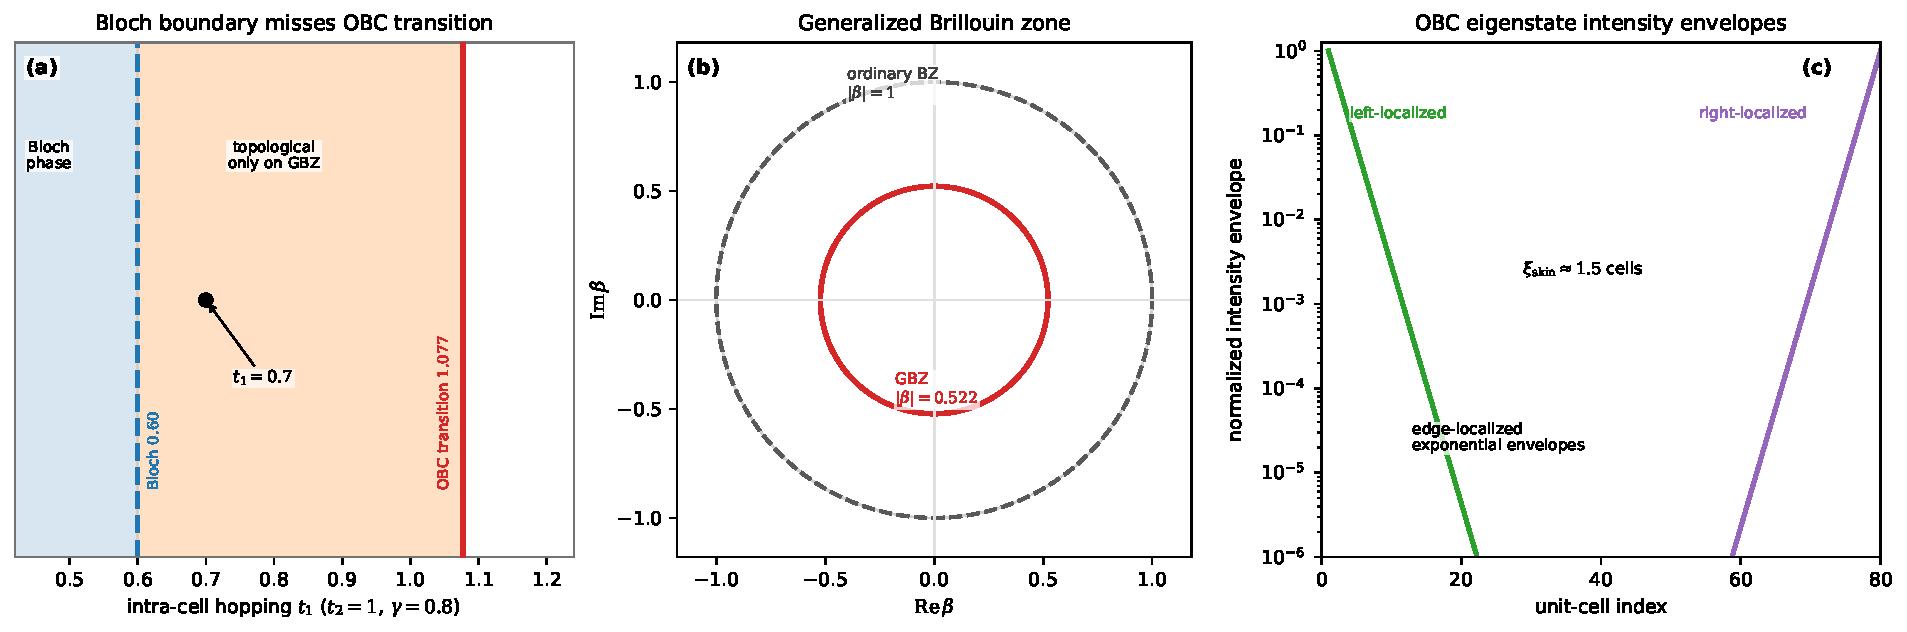
\includegraphics[width=0.98\linewidth]{fig_f15_non_bloch_bbc.pdf}
 \caption{Failure of the Bloch bulk-boundary correspondence and its
 non-Bloch resolution for the non-Hermitian SSH model with $t_2 = 1$
 and $\gamma = 0.8$.
 (a)~One-parameter phase strip. The dashed blue line marks the
 Bloch/PBC phase boundary at $t_1 = 0.60$; the solid red line marks
 the true OBC/GBZ transition at $t_1 = 1.077$. The orange region
 between them is topologically nontrivial only on the generalised
 Brillouin zone---a qualitative failure of the conventional Bloch
 invariant. The black dot marks $t_1 = 0.7$, the parameter used in
 panels~(b) and~(c).
 (b)~Generalised Brillouin zone in the complex $\beta$ plane. The
 dashed grey circle is the ordinary BZ ($|\beta| = 1$); the solid
 red circle is the GBZ with $|\beta| = 0.522$, computed from the
 transfer-matrix eigenvalue condition.
 (c)~Normalised intensity envelopes of representative OBC zero modes on
 a logarithmic scale. Green and purple mark modes localised at the two
 terminations. The decay is exponential with
 skin length $\xi_{\mathrm{skin}} = -1/\ln|\beta_{\mathrm{GBZ}}|
 \approx 1.54$ unit cells. Curves are clipped below $10^{-6}$ for
 display.}
 \label{fig:ch15-non-bloch-bbc}
\end{figure}


%% ================================================================
\section{The non-Bloch bulk-boundary correspondence}
\label{sec:non-bloch-bbc}

The resolution, introduced by Yao and Wang, is to compute topological
invariants on the generalized Brillouin zone
(Section~\ref{sec:gbz})---the contour in the complex $\beta$ plane
that correctly describes the open-boundary eigenstates.

\subsection{Statement}
\label{ssec:non-bloch-statement}

For a one-dimensional non-Hermitian system with chiral symmetry, the
\emph{non-Bloch bulk-boundary correspondence}~\cite{yao2018edge,yokomizo2019non,yang2020non} states:
\begin{equation}
 \boxed{
 N_{\mathrm{zero\;modes\;per\;interface}} = |\wnum_{\mathrm{GBZ}}|,
 }
 \label{eq:non-bloch-bbc}
\end{equation}
where $\wnum_{\mathrm{GBZ}}$ is the winding number computed on the
GBZ~\eqref{eq:non-bloch-winding}. For a finite SSH chain with two
topological terminations, the total number of zero modes is therefore
twice this value. This invariant correctly predicts the topological zero
modes throughout the gapped parameter regime, including where the
conventional Bloch invariant gives the wrong answer.

\subsection{The GBZ for the non-Hermitian SSH model}
\label{ssec:gbz-ssh}

For the non-Hermitian SSH model~\eqref{eq:nh-ssh-bloch}, replacing
$e^{ik} \to \beta$ yields the characteristic equation
\begin{equation}
 (t_1 + \gamma/2 + t_2\,\beta^{-1})(t_1 - \gamma/2 + t_2\,\beta) = E^2.
 \label{eq:nh-ssh-char}
\end{equation}
At $E = 0$ (the gap-closing energy for chiral-symmetric systems), this
gives four solutions for $\beta$. Ordering them by modulus,
$|\beta_1| \le |\beta_2| \le |\beta_3| \le |\beta_4|$, the GBZ
condition~\eqref{eq:gbz-condition} requires $|\beta_2| = |\beta_3|$.

For this model, the GBZ is a circle of radius
\begin{equation}
  |\beta_{\mathrm{GBZ}}| = r
  = \sqrt{\frac{|t_1 - \gamma/2|}{|t_1 + \gamma/2|}}.
  \label{eq:gbz-radius-ssh}
\end{equation}
The final equality assumes the positive real parameter regime used in the
example.  The intercell hopping $t_2$ sets the overall frequency
scale for this symmetric intercell choice and therefore does not affect
the GBZ radius.  In the Hermitian limit $\gamma=0$, the radius becomes
$r=1$, so the GBZ reduces continuously to the ordinary Brillouin zone.
The GBZ-based winding number is computed by evaluating $h(\beta)$ on this
deformed contour rather than on the unit circle.

\subsection{Derivation of the non-Bloch BBC}
\label{ssec:bbc-derivation}

The key idea is that the open-boundary eigenstates at zero energy are
determined by the transfer-matrix eigenvalues at $E = 0$. For a chain
of $L$ unit cells, a zero-energy eigenstate must satisfy the boundary
conditions at both the left and right ends. Writing the spatial
dependence as a sum of the four transfer-matrix solutions
$\psi_n \sim \sum_j c_j\,\beta_j^n$, normalizability imposes constraints
from both boundaries.

From the left boundary, the coefficients of the solutions that grow
toward the left ($|\beta_j| > 1$ when viewed from the left end) must
vanish; otherwise $|\psi_n|$ would diverge as $n \to \infty$.
Similarly, from the right boundary, the coefficients of the solutions
that grow toward the right ($|\beta_j| < 1$ when viewed from the right
end) must vanish from the right-end perspective. For a system with
$2n$ transfer-matrix eigenvalues ordered by modulus
$|\beta_1| \le |\beta_2| \le \cdots \le |\beta_{2n}|$, a normalizable
zero mode exists precisely when the boundary conditions can be
simultaneously satisfied---that is, when exactly $n$ eigenvalues lie
inside the GBZ contour and $n$ lie outside.

The GBZ contour is defined by the condition $|\beta_n| = |\beta_{n+1}|$:
the two ``middle'' eigenvalues must have equal modulus. This is
because the zero mode at the interface between the inside and outside
groups must change character precisely at the GBZ radius. When this
condition holds, the transfer-matrix problem has a self-consistent
solution that is normalizable from both ends simultaneously.

As parameters are varied, a zero mode appears or disappears when a
$\beta_j$ \emph{crosses the GBZ contour}---not when it crosses the unit
circle. The winding number computed on the GBZ counts how many times
this crossing has occurred, and therefore correctly predicts the number
of topological zero modes.

\paragraph{Physical interpretation of the GBZ radius.}
The GBZ radius $r = |\beta_{\mathrm{GBZ}}|$ has a direct physical
meaning: it determines the \emph{skin localisation length}
\begin{equation}
 \xi_{\mathrm{skin}} = \frac{-1}{\ln r},
 \label{eq:skin-length-from-gbz}
\end{equation}
measured in unit cells. When $r < 1$, the bulk skin states are
exponentially localised toward the left boundary with decay length
$\xi_{\mathrm{skin}}$; when $r > 1$, they localise toward the right.
In the Hermitian limit $r \to 1$, $\xi_{\mathrm{skin}} \to \infty$ and
the bulk modes become extended Bloch waves.

For the non-Hermitian SSH model with $t_2 = 1$ and $\gamma = 0.8$, the
GBZ radius is $r = 0.522$ (Figure~\ref{fig:ch15-non-bloch-bbc}b),
giving a skin length $\xi_{\mathrm{skin}} = 1/|\ln 0.522| \approx
1.54$ unit cells---an extremely strong localisation. This quantitative
prediction can be tested directly by measuring the spatial decay of the
field envelope in a finite photonic lattice, as demonstrated in
microwave waveguide networks and acoustic metamaterials.

\paragraph{GBZ for general two-band models.}
The GBZ construction generalises straightforwardly to any two-band
non-Hermitian model with nearest-neighbour coupling. The Bloch
Hamiltonian takes the form
$H(\beta) = \sum_j d_j(\beta)\,\sigma_j$ where
$d_j(\beta) = d_j^{(0)} + d_j^{(+)}\beta + d_j^{(-)}\beta^{-1}$.
The characteristic equation $\det(E - H(\beta)) = 0$ is a polynomial
in $\beta$ (typically quartic for two-band models), and the GBZ is
the contour in the complex $\beta$ plane on which the middle pair
of roots has equal modulus. For models with only one asymmetric
hopping parameter (such as the Hatano--Nelson model), the GBZ is a
circle and the calculation reduces to finding a single radius $r$.
For models with multiple asymmetric parameters, the GBZ can be a
non-circular closed curve, and the winding number must be computed
numerically by discretising the GBZ contour and tracking the phase
of $\det H(\beta)$. The algorithms for this computation are
discussed in Chapter~\ref{ch:numerics}.

\begin{remark}
The derivation shows why the \emph{shape} of the GBZ matters, not just
its existence. For models where the GBZ is not a circle (e.g.,
multi-band or long-range hopping models), the contour can be
self-intersecting or multi-sheeted, and the winding number must be
computed on the full geometric GBZ rather than a simple circle.
\end{remark}


%% ================================================================
\section{Example: non-Hermitian SSH phase diagram}
\label{sec:nh-ssh-example}

To make the non-Bloch BBC concrete, consider the non-Hermitian SSH
model with $t_2 = 1$ and $\gamma = 0.8$.

\subsection{Bloch versus non-Bloch phase boundaries}
\label{ssec:phase-boundaries}

The conventional Bloch winding number predicts a topological phase
transition at $|t_1 + 0.4| = 1$, i.e., $t_1 = 0.6$ or $t_1 = -1.4$.
The non-Bloch winding number, computed on the GBZ, predicts a
transition at $t_1 = \sqrt{1 + 0.16} \approx 1.077$. These are
quantitatively different---the Bloch prediction misplaces the phase
boundary by nearly a factor of two.

\subsection{OBC spectrum and edge states}
\label{ssec:obc-edge}

Exact diagonalization of an open chain of $L = 60$ unit cells confirms
the non-Bloch prediction. For $t_1 = 0.8$ (between the Bloch and
non-Bloch boundaries), the Bloch invariant gives $\wnum = 0$ (trivial),
but the OBC spectrum shows two robust zero-energy edge states. For
$t_1 = 1.2$ (above the non-Bloch boundary), the edge states vanish.

This example demonstrates that the non-Bloch BBC is essential for
predicting the topological phase diagram of non-Hermitian systems with
the skin effect.


%% ================================================================
\section{Biorthogonal bulk-boundary correspondence}
\label{sec:biorthogonal-bbc}

An alternative approach to rebuilding the bulk-boundary correspondence
uses the \emph{biorthogonal polarization}---a non-Hermitian
generalization of the electric polarization or Zak phase.

\subsection{Biorthogonal polarization}
\label{ssec:biorthogonal-pol}

In a Hermitian system, the bulk polarization is defined as the integral
of the Berry connection over the Brillouin zone. In a non-Hermitian
system, the biorthogonal polarization uses the left and right
eigenvectors:
\begin{equation}
 P^{\mathrm{bi}} = \frac{1}{2\pi}\oint_{\BZ}
 i\,\frac{\langle u_k^{\mathrm{L}}|\partial_k|u_k^{\mathrm{R}}\rangle}
 {\langle u_k^{\mathrm{L}}|u_k^{\mathrm{R}}\rangle}\;\dd k.
 \label{eq:biorthogonal-pol}
\end{equation}
This quantity is quantized (modulo integers) by chiral symmetry and
predicts the existence of edge states in the biorthogonal
framework.

\begin{figure}[t]
 \centering
 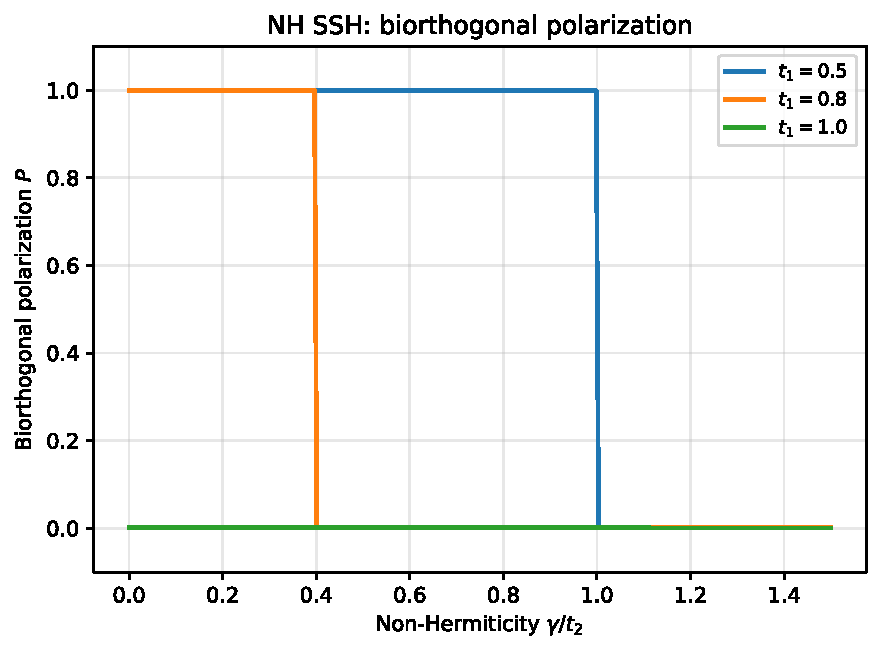
\includegraphics[width=0.6\linewidth]{figures/fig_f15_biorthogonal_pol.pdf}
 \caption{Biorthogonal polarization diagnostic as a function of
 non-Hermiticity $\gamma/t_2$ for different intracell hoppings $t_1$ in
 the NH SSH model. The plotted convention uses values $0$ and $1$ for
 the two quantized sectors; in the usual polarization convention these
 correspond to $P=0$ and $P=1/2$ modulo one. The jump marks the
 non-Hermitian topological transition in this biorthogonal diagnostic.
 Chiral symmetry pins the value to a quantized sector away from gap
 closings.}
 \label{fig:biorthogonal-pol}
\end{figure}

\subsection{Physical interpretation}
\label{ssec:biorthogonal-interpretation}

The biorthogonal polarization has a direct physical interpretation.
In a Hermitian system, the bulk polarization measures the displacement
of charge (or field energy) within the unit cell. In a non-Hermitian
system, $P^{\mathrm{bi}}$ measures the displacement of the
\emph{biorthogonal} charge density $\rho^{\mathrm{bi}}(x) =
\langle\psi^{\mathrm{L}}(x)|\psi^{\mathrm{R}}(x)\rangle$, which
can be complex. The quantization of $P^{\mathrm{bi}}$ reflects the
fact that a half-integer displacement of the biorthogonal charge
(modulo one) signals a topological phase with boundary-localized
modes.

\paragraph{Example: biorthogonal polarisation of the NH SSH model.}
For the non-Hermitian SSH model~\eqref{eq:nh-ssh-bloch} with
$t_1 = 0.5$, $t_2 = 1$, $\gamma = 0.6$, the right eigenvector of the
lower band is
$|u_k^{\mathrm{R}}\rangle = (1,\; -E(k)/h(k))^\transpose$ (up to
normalisation and branch convention), where $E(k) = \sqrt{h(k)\tilde{h}(k)}$,
$h(k) = t_1 + \gamma/2 + t_2 e^{-ik}$, and
$\tilde{h}(k) = t_1 - \gamma/2 + t_2 e^{ik}$. The left eigenvector is
obtained from the transpose/adjoint eigenproblem with the corresponding
left-right normalization. Numerical integration of the biorthogonal
connection, or equivalently the non-Bloch version evaluated on the GBZ
when skin modes are present, gives the quantized topological sector.
For this parameter set the polarization is in the topological sector
($P=1/2$ modulo one in the usual convention). When $t_1$ is increased
past the non-Bloch transition
($t_1 = \sqrt{t_2^2 + (\gamma/2)^2} = \sqrt{1.09} \approx 1.044$),
the non-Bloch/biorthogonal diagnostic jumps discontinuously to the trivial sector
(trivial), in agreement with the non-Bloch winding number. The jump
is sharp---not a smooth crossover---because $P^{\mathrm{bi}}$ is
quantised by chiral symmetry.

This confirms that the biorthogonal polarisation and the non-Bloch
winding number are two faces of the same topological invariant: they
detect the same phase transitions and predict the same edge states,
but provide different physical pictures---one based on GBZ deformation,
the other on biorthogonal charge displacement.

\subsection{Connection to QNM inner products}
\label{ssec:biorthogonal-qnm}

The biorthogonal polarization~\eqref{eq:biorthogonal-pol} is closely~\cite{kunst2018biorthogonal}
related to the unconjugated inner product used for quasinormal modes
(Section~\ref{sec:qnm-adjoint}). In both cases, the key mathematical
structure is the pairing between left (adjoint) and right eigenstates.
For a photonic system described by the Maxwell operator
$\hat{\Theta}$, the biorthogonal Berry connection becomes
\begin{equation}
 A_k^{\mathrm{bi}} = i\,
 \frac{\langle\tilde{\EE}_k^{\mathrm{L}}|
 \partial_k|\tilde{\EE}_k^{\mathrm{R}}\rangle_{\varepsilon}}
 {\langle\tilde{\EE}_k^{\mathrm{L}}|
 \tilde{\EE}_k^{\mathrm{R}}\rangle_{\varepsilon}},
 \label{eq:biorthogonal-berry-bbc}
\end{equation}
where $\langle\cdot|\cdot\rangle_\varepsilon$ is the unconjugated
inner product weighted by the permittivity tensor. This connects the
topological classification of non-Hermitian photonic bands directly to
the QNM formalism of Chapter~\ref{ch:qnm}.

\subsection{Relation to the non-Bloch approach}
\label{ssec:bbc-comparison}

The biorthogonal and non-Bloch approaches give consistent predictions
when the inner product and integration contour are chosen for the same
boundary problem, but they emphasize complementary physical insights:
\begin{itemize}
 \item The \textbf{non-Bloch approach} directly accounts for the
 skin effect by deforming the integration contour; it gives the
 correct phase diagram and the correct localization properties
 of edge states.
 \item The \textbf{biorthogonal approach} replaces the inner product
 with a left-right one and is more closely connected to the formalism
 of Chapter~\ref{ch:qnm} and the adjoint modes of the Maxwell operator.
 When the skin effect is present, its bulk version must be combined
 with the non-Bloch contour or with open-boundary biorthogonal states.
 \item For systems \emph{without} the skin effect (e.g., systems with
 reciprocity or additional symmetries that prevent the spectral
 loop from winding), the biorthogonal approach may be the only
 relevant non-Hermitian correction.
 \item For systems \emph{with} the skin effect, both approaches are
 needed for a complete picture: the non-Bloch approach gives the
 correct phase diagram, and the biorthogonal approach clarifies
 the physical meaning of the topological invariant.
\end{itemize}


%% ================================================================
\section{Higher-dimensional correspondence}
\label{sec:bbc-higher-d}

In two and higher dimensions, rebuilding the bulk-boundary
correspondence requires both non-Bloch band theory and the spectral-area
diagnostics discussed in Chapter~\ref{ch:point-gap}~\cite{zhang2022universal}.

\subsection{Non-Bloch Chern insulator}
\label{ssec:non-bloch-chern-insulator}

For a two-dimensional non-Hermitian Chern insulator, the non-Bloch Chern
number (Section~\ref{ssec:non-bloch-chern}) correctly predicts the
number of chiral edge modes, which can differ from the prediction of the
conventional Chern number when the skin effect is present.

The construction is conceptually straightforward: the two-dimensional
GBZ is the product of two one-dimensional GBZ contours (one for each
reciprocal direction), and the non-Bloch Chern number is the integral
of the Berry curvature over this deformed torus. In practice, computing
the two-dimensional GBZ is more involved because the GBZ contour in
each direction can depend on the momentum in the other direction.

\subsection{Corner modes and higher-order topology}
\label{ssec:corner-modes}

In certain two-dimensional systems, an extensive set of eigenstates can
be localized at
\emph{corners} rather than edges---the corner-skin effect
(Section~\ref{sec:skin-2d}). The relevant topological invariant is a
second-order non-Bloch invariant, defined by a nested GBZ construction:
first compute the GBZ in one direction at fixed momentum in the other,
then compute a one-dimensional topological invariant on the resulting
edge theory.

The corner modes predicted by this construction are exponentially
localized at zero, one, or two corners of a rectangular sample, depending
on the non-Bloch invariant and the orientation of the skin effect.

\subsection{Geometry dependence}
\label{ssec:geometry-dependence}

The geometry-dependent skin effect (Section~\ref{sec:skin-2d}) means that
the bulk-boundary correspondence itself can depend on the sample shape.
For example, a hexagonal sample may exhibit edge states on some edges but
not others, depending on the orientation of the non-reciprocal hopping.
This shape dependence has no Hermitian counterpart and requires a
boundary-condition-aware formulation of the topological invariant.


%% ================================================================
\section{Photonic implications}
\label{sec:bbc-photonic}

For photonic systems described by the Maxwell equations, the rebuilt
bulk-boundary correspondence has several practical implications.

\subsection{Photonic GBZ construction}
\label{ssec:photonic-gbz}

For a 1D non-Hermitian photonic system with effective nonreciprocal or
non-unimodular evolution, the GBZ can be constructed directly from the
Maxwell transfer matrix without passing through a tight-binding
approximation. The procedure is:
\begin{enumerate}
 \item Compute the unit-cell transfer matrix $M(\omega)$ at each
 complex frequency $\omega$ using the complex-$n_j$ layer
 propagation matrices of Chapter~\ref{ch:point-gap}.
 \item Find the eigenvalues $\beta_{1,2}(\omega)$ of $M(\omega)$.
 \item The GBZ is the corresponding contour in the complex $\beta$
 plane where the middle transfer-matrix roots have equal modulus; for a
 two-root problem this condition is $|\beta_1(\omega)|=|\beta_2(\omega)|$.
 \item On this contour, evaluate the photonic topological invariant
 (winding number or biorthogonal polarisation).
\end{enumerate}
For a reciprocal isotropic layer stack described by the usual
two-component field vector, the unit-cell transfer matrix is unimodular
even with material loss or gain. Then $\beta_1\beta_2=1$, and the
condition $|\beta_1|=|\beta_2|$ reduces to $|\beta_1|=|\beta_2|=1$.
Complex permittivity can still produce complex bands and evanescent
solutions, but it does not by itself generate a Hatano--Nelson-type GBZ
deformation. A genuine photonic non-Bloch correction requires an
effective evolution that breaks this cancellation, for example through
magneto-optical bias, temporal modulation, cascaded reservoirs, or a
multi-port network after unobserved channels are eliminated.

\paragraph{Connection to the photonic transfer-matrix formalism.}
The photonic GBZ construction links directly to the transfer-matrix
band theory of Chapter~\ref{ch:periodicity}: the Bloch condition
$\cos(Ka)=\xi(\omega)$ is replaced, in the effective nonreciprocal
problem, by the middle-root condition defining the GBZ. Instead of
solving only for real $K$ on the unit circle, one solves for the complex
$K$ values that reproduce the open-boundary spectrum. This makes the
non-Bloch theory of photonic topological phases accessible to the same
transfer-matrix and scattering tools used routinely in multilayer and
coupled-resonator design, provided the effective model includes the
channels responsible for directional gain or hopping.

\subsection{Design of robust edge channels}
\label{ssec:robust-edge}

In a non-Hermitian photonic crystal, edge channels designed using
conventional (Bloch) topological invariants may not appear or may appear
at unexpected parameter values. The non-Bloch approach provides a
concrete design rule: compute the GBZ for the target structure, evaluate
the topological invariant on the GBZ, and verify the edge-state
prediction against finite-structure simulations. This ensures that
the designed edge states are robust and correctly placed.

The practical difficulty is that computing the photonic GBZ requires
solving the Maxwell transfer matrix at complex frequencies and complex
wave vectors---a task that goes beyond standard photonic band-structure
calculations but is within the reach of the numerical methods of
Chapter~\ref{ch:numerics}.

\subsection{Directional amplification}
\label{ssec:directional-amp}

The skin effect combined with edge-state topology enables
\emph{topological amplifiers}: devices where light injected at one
boundary is amplified while propagating along an edge channel,
with directionality set by the non-Bloch topology and by the engineered
gain profile. The amplification can scale exponentially over the useful
device length, but in a physical photonic structure it is limited by
saturation, radiation loss, and disorder-induced mode mixing rather than
being absolutely immune to backscattering.

\subsection{Spectral engineering}
\label{ssec:spectral-engineering}

The dramatic difference between PBC and OBC spectra in non-Hermitian
photonic crystals can be exploited for spectral engineering. By
choosing boundary conditions (periodic, open, or mixed), the same
photonic structure can exhibit qualitatively different spectral
properties. For example, a ring resonator (PBC) and a terminated
waveguide array (OBC) made from the same non-Hermitian photonic crystal
will have different resonance frequencies, different mode spacings, and
different field distributions.

\subsection{Experimental signatures}
\label{ssec:experimental-signatures}

The non-Bloch BBC makes testable predictions for photonic experiments:
\begin{enumerate}
 \item \textbf{Edge-state presence:} the appearance or disappearance
 of edge modes as a function of gain/loss or coupling asymmetry
 should follow the non-Bloch phase boundary, not the Bloch one.
 \item \textbf{Spectral collapse:} the PBC-to-OBC spectral change
 (Figure~\ref{fig:skin-pbc-obc-spectra}) is a direct observable
 in coupled-resonator experiments where periodic or open boundary
 conditions can be implemented.
 \item \textbf{GBZ deformation:} the GBZ radius
 (Figure~\ref{fig:gbz-circle}) manifests as the exponential
 envelope of the skin modes, which can be measured from the
 spatial intensity profile.
\end{enumerate}

\paragraph{Edge-state penetration depth.}
In the non-Hermitian SSH model used in Fig.~\ref{fig:edge-localisation},
$t_1 = 0.6$, $t_2 = 1.0$, and the nonreciprocal hopping parameter is
$\delta = 0.3$.  The right zero mode on sublattice A obeys the open-chain
recursion
\begin{equation}
  (t_1-\delta)A_n + (t_2+\delta)A_{n+1}=0,
  \qquad
  \frac{|A_{n+1}|}{|A_n|}=\left|\frac{t_1-\delta}{t_2+\delta}\right|,
  \label{eq:edge-recursion}
\end{equation}
so the amplitude penetration depth is
\begin{equation}
  \xi_{\mathrm{edge}}
  = \frac{1}{\ln\left|(t_2+\delta)/(t_1-\delta)\right|}
  = \frac{1}{\ln(1.3/0.3)}
  \approx 0.68\;\text{cells}.
  \label{eq:edge-penetration}
\end{equation}
The Hermitian estimate obtained by setting $\delta=0$ is
$\xi_{\mathrm{Herm}}=1/\ln|t_2/t_1|\approx1.96$ cells, but that estimate
ignores the nonreciprocal intracell/intercell imbalance.  The non-Bloch
calculation and the direct OBC eigenvector therefore agree: the edge mode
is much more tightly confined than the Hermitian SSH formula would
suggest.  The exponential envelope $\propto e^{-x/\xi_{\mathrm{edge}}}$
has been confirmed experimentally in coupled-resonator arrays at both
microwave and optical frequencies, where the spatial intensity profile of
the edge mode can be measured site by site.

\begin{figure}[t]
 \centering
 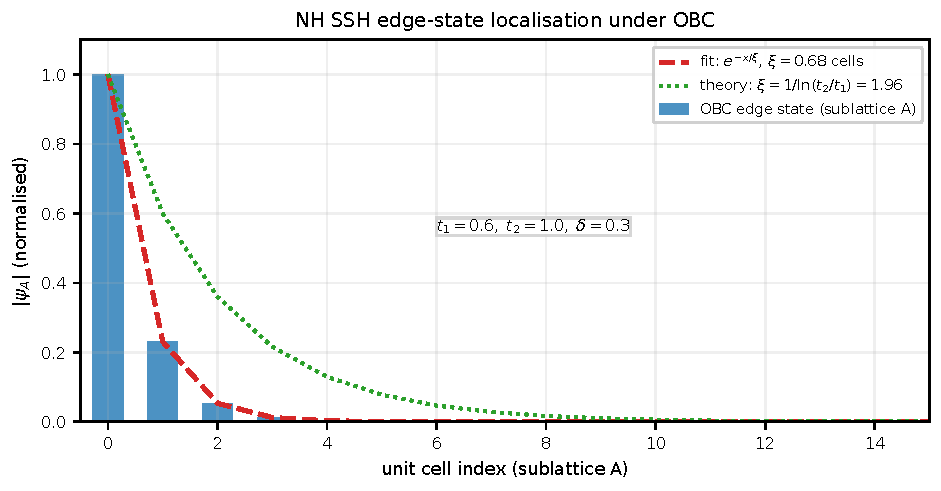
\includegraphics[width=0.82\linewidth]{fig_f15_edge_localisation.pdf}
  \caption{Sublattice-A amplitudes of the zero-energy edge state in
  the non-Hermitian SSH model ($t_1 = 0.6$, $t_2 = 1.0$,
  $\delta = 0.3$) under open boundary conditions, normalized to the
  boundary site. Red dashed: exponential fit to the first eight sites
  gives $\xi_{\mathrm{fit}} \approx 0.68$ cells, in agreement with the
  nonreciprocal zero-mode recursion~\eqref{eq:edge-recursion}. Green
  dotted: the Hermitian estimate
  $\xi_{\mathrm{Herm}} = 1/\ln(t_2/t_1) \approx 1.96$ cells, which
  ignores the hopping asymmetry $\delta$. The discrepancy is therefore
  not a plotting artifact but the edge-state analogue of the non-Bloch
  correction: the correct decay length follows from the open-boundary
  recursion or, equivalently, from the generalized Brillouin zone.}
 \label{fig:edge-localisation}
\end{figure}

\begin{figure}[t]
 \centering
 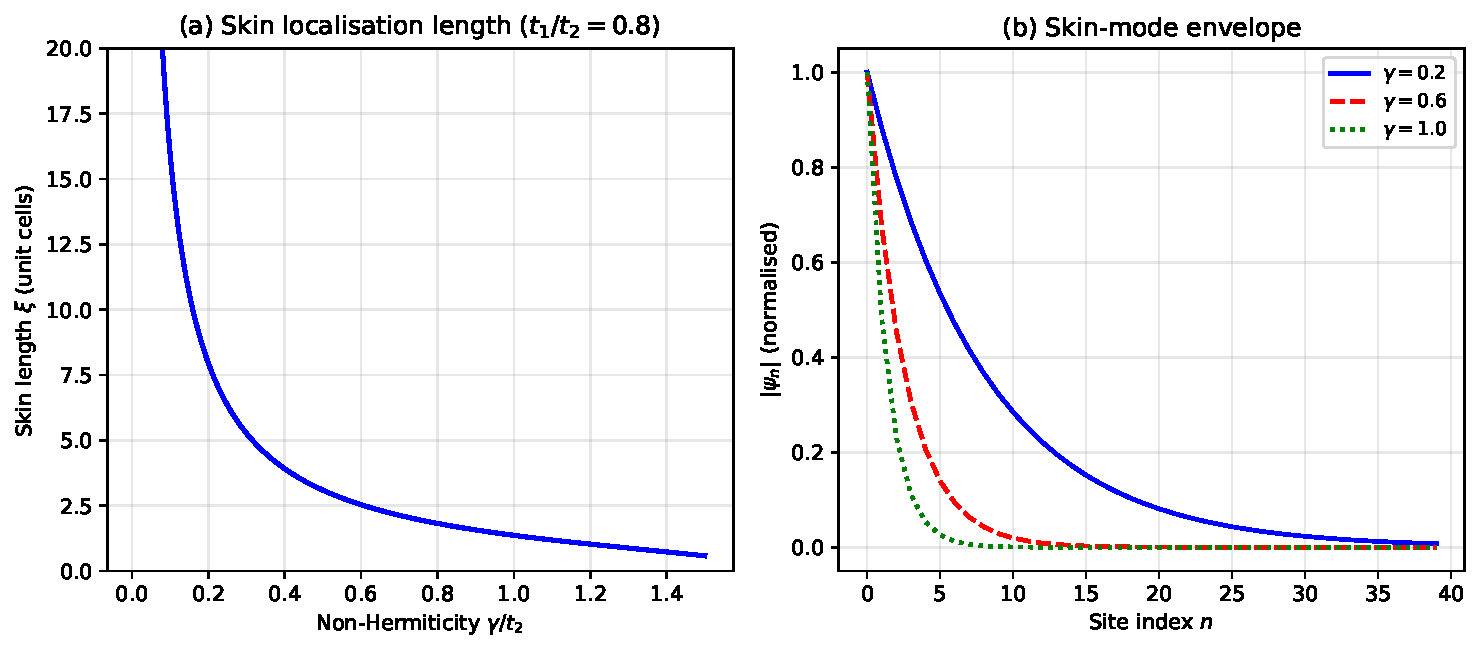
\includegraphics[width=0.85\linewidth]{figures/fig_f15_edge_penetration.pdf}
 \caption{Skin-effect localisation in the NH SSH model
 ($t_1/t_2 = 0.8$).
 (a)~Skin localisation length $\xi$ as a function of the
 non-Hermiticity parameter $\gamma$: $\xi$ diverges as
 $\gamma \to 0$ (Hermitian limit, where all bulk modes become
 extended) and decreases monotonically with increasing asymmetry.
 (b)~Skin-mode envelope $|\psi_n|$ for three values of $\gamma$,
 showing progressively stronger localisation toward one boundary
 as the non-Hermiticity grows.}
 \label{fig:edge-penetration}
\end{figure}

\paragraph{Experimental verification at optical frequencies.}
Photonic and microwave coupled-resonator experiments can test the
non-Bloch BBC by comparing spectra under ring-closed and ring-terminated
boundary conditions. The key checks are qualitative and quantitative:
the measured phase boundary should follow the GBZ prediction, and the
observed edge-mode localisation length should match the open-boundary
recursion or Eq.~\eqref{eq:edge-penetration} within fabrication
tolerance. Such measurements would test the non-Bloch correction to the
topological properties of non-Hermitian photonic systems.

\begin{takeaway}[The bulk-boundary correspondence survives]
The bulk-boundary correspondence is not destroyed by non-Hermiticity---it
is transformed. In its rebuilt form, it connects topological invariants
computed on the generalized Brillouin zone (or using biorthogonal inner
products) to the edge-state structure of open non-Hermitian systems.
The correspondence remains exact and robust, but it requires the non-Bloch
theory of Chapter~\ref{ch:skin-effect}: the unit circle is no longer the
correct Brillouin zone, the Bloch winding number is no longer the correct
invariant, and the Bloch phase diagram is no longer the correct map.
Once these replacements are made, the deep connection between bulk
topology and boundary physics is fully restored.
\end{takeaway}

\chapter{Bound States in the Continuum and Exceptional Topology}
\label{ch:bic-topology}

\begin{chapterlead}
Not all non-Hermitian phenomena involve complex eigenfrequencies. A
\emph{bound state in the continuum} (BIC)~\cite{hsu2016bound,koshelev2018nonradiating,kang2023applications,koshelev2018asymmetric,kang2022merging,bai2024recovery,gao2024degenerate} is a mode with a real
eigenfrequency embedded within the radiation continuum---a state that,
by symmetry or fine-tuning, is perfectly decoupled from all outgoing
channels despite coexisting spectrally with radiation modes. BICs often
behave as topological objects: in photonic crystal slabs with a
well-defined far-field polarization, they carry quantized charges in
momentum space and can be connected to exceptional points through the
analytic structure of open-system resonances. The BIC condition is
derived from the Maxwell problem, the role of topological charge is
identified, and photonic crystal slabs serve as the main examples.
\end{chapterlead}


%% ================================================================
\section{What is a bound state in the continuum?}
\label{sec:bic-definition}

In an open photonic structure---a photonic crystal slab, a grating, or
a metasurface---most resonances are quasinormal modes with complex
frequencies $\omtil = \omega - i\gamma$ and finite quality factors
(Chapter~\ref{ch:qnm}). A BIC is the exception: it has $\gamma = 0$
(infinite $\Qfac$) despite lying within the frequency range where
radiation channels are open.

Formally, a BIC is a normalizable solution of the source-free Maxwell
equations at a real frequency $\omega_{\mathrm{BIC}}$ that satisfies
$\omega_{\mathrm{BIC}} > \omega_{\mathrm{light\;line}}$---above the
light line, where radiation modes exist---yet has zero coupling to all
radiation channels.

\subsection{The radiation-amplitude viewpoint}
\label{ssec:radiation-amplitude}

To make the BIC condition precise within the Maxwell framework, consider
a photonic crystal slab of thickness $d$ with in-plane periodicity. At
each Bloch wave vector $\kk_\parallel$ and frequency $\omega$, the
far-field radiation above and below the slab can be decomposed into a
finite number of open diffraction channels, each carrying a transverse
polarization. Let $c_j(\kk_\parallel)$ denote the complex amplitude
radiated into channel $j$. The total radiation rate is
\begin{equation}
 \gamma(\kk_\parallel) \propto \sum_j |c_j(\kk_\parallel)|^2.
 \label{eq:radiation-rate}
\end{equation}
A BIC occurs when every \emph{open} radiation amplitude vanishes
simultaneously:
\begin{equation}
 c_j(\kk_{\mathrm{BIC}}) = 0 \quad \text{for all open channels } j.
 \label{eq:bic-all-zero}
\end{equation}
This is a set of conditions---one complex equation per independent
channel amplitude, modulo symmetry and phase constraints---so generic
BICs normally require tuning. At high-symmetry points where symmetry
forbids certain channels, fewer conditions remain and BICs arise more
naturally.

\subsection{Symmetry-protected BICs}
\label{ssec:symmetry-bic}

A symmetry-protected BIC exists at high-symmetry points in the Brillouin
zone (e.g., $\Gamma$) where the mode belongs to an irreducible
representation that is incompatible with the radiation continuum. For
example, a mode that is odd under a $C_2$ rotation of the slab cannot
couple to normally incident plane waves, which transform as the trivial
representation. The decoupling is exact and persists under any
perturbation that preserves the symmetry.

At the $\Gamma$ point of a square-lattice photonic crystal slab, the
point group is $C_{4v}$. Modes belonging to the $B_1$ or $B_2$
representations are incompatible with the $s$- and $p$-polarized plane
waves (which belong to $A_1$ and $E$), ensuring zero radiation. Moving
away from $\Gamma$ reduces the symmetry, and the mode acquires a finite
radiation rate---becoming a quasi-BIC with high but finite $\Qfac$.

\subsection{Accidental (tuned) BICs}
\label{ssec:accidental-bic}

At generic $\kk$-points away from high-symmetry positions, BICs can
arise from a destructive interference between two or more radiation
channels. These accidental BICs require fine-tuning of one structural
parameter (e.g., the slab thickness, hole radius, or lattice constant)
and are generically isolated points in the $(\kk, \text{parameter})$
space.

Near an accidental BIC, the radiation amplitudes vanish linearly:
$c_j \propto |\kk - \kk_{\mathrm{BIC}}|$. Since $\gamma \propto
\sum |c_j|^2$, the quality factor diverges as
\begin{equation}
 \Qfac(\kk) \propto \frac{1}{|\kk - \kk_{\mathrm{BIC}}|^2},
 \label{eq:bic-Q-divergence}
\end{equation}
producing a family of ultra-high-$\Qfac$ quasi-BIC resonances in the
vicinity.
\begin{figure}[t]
 \centering
 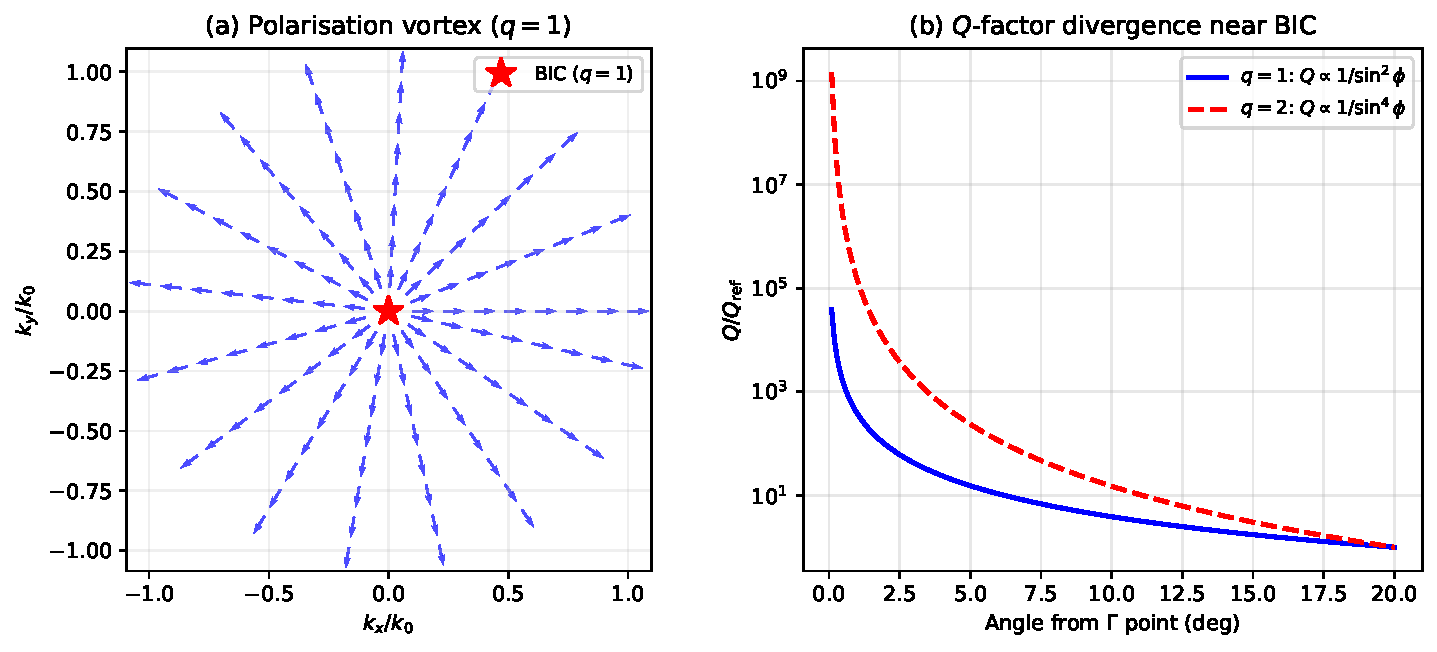
\includegraphics[width=0.85\linewidth]{figures/fig_f16_bic_farfield.pdf}
 \caption{Far-field polarization vortex and quality-factor divergence
 near a symmetry-protected BIC. (a)~The polarization direction winds
 once around the BIC in momentum space, giving topological charge
 $q=1$. (b)~The radiative quality factor diverges as the far-field
 radiation amplitude vanishes; higher-charge vortices produce steeper
 $Q$-scaling. This figure connects the Maxwell radiation amplitudes
 $c_j(\kk)$ in Eq.~\eqref{eq:radiation-rate} to the polarization
 topology used to classify BICs.}
 \label{fig:bic-farfield-vortex}
\end{figure}


\subsection{Other BIC mechanisms}
\label{ssec:other-bic}

Beyond symmetry protection and parametric tuning, BICs can also arise
through Fabry--P\'erot interference (standing waves in the slab thickness
direction that decouple from radiation), Friedrich--Wintgen avoided
crossing (two resonances exchanging their radiation channels so that one
becomes dark), and inverse-construction methods that engineer the
potential or hopping rates to produce a bound state at a desired
location~\cite{wang2023brillouin}. The common thread is the vanishing
of all radiation amplitudes~\eqref{eq:bic-all-zero}.

\subsection{Friedrich--Wintgen avoided crossing}
\label{ssec:friedrich-wintgen}

A particularly instructive BIC mechanism arises from the avoided crossing
of two resonances coupled through a shared radiation continuum. Consider
two quasi-bound modes $|1\rangle$ and $|2\rangle$ with complex frequencies
$\omtil_j = \omega_j - i\gamma_j$ that approach each other as a structural
parameter is varied. In the two-mode TCMT of
Chapter~\ref{ch:maxwell-coupled-modes}, the effective Hamiltonian including
radiation coupling is
\begin{equation}
 H_{\mathrm{FW}} =
 \begin{pmatrix}
 \omega_1 - i\gamma_1 & \kappa - i\sqrt{\gamma_1\gamma_2}\,e^{i\phi} \\
 \kappa - i\sqrt{\gamma_1\gamma_2}\,e^{-i\phi} & \omega_2 - i\gamma_2
 \end{pmatrix},
 \label{eq:fw-hamiltonian}
\end{equation}
where $\kappa$ is the near-field coupling and the off-diagonal imaginary
term represents far-field coupling mediated by the shared continuum, with
relative phase $\phi$. Friedrich and Wintgen showed that there exists a
parameter value at which one eigenvalue becomes purely real: the radiation
widths of the two modes rearrange so that one mode absorbs all the
radiation and the other becomes a BIC with $\gamma = 0$.

In this two-mode model the Friedrich--Wintgen BIC occurs when the dark
eigenvector is orthogonal to the continuum-coupling vector. For the
phase convention of Eq.~\eqref{eq:fw-hamiltonian}, this can be written
schematically as
\begin{equation}
 \frac{\kappa}{\sqrt{\gamma_1\gamma_2}} = \frac{\omega_1 - \omega_2}{\gamma_1 - \gamma_2}\,\sin\phi,
 \label{eq:fw-condition}
\end{equation}
with the precise form depending on the normalization of the radiative
coupling amplitudes. The essential requirement is destructive
interference of the two radiative pathways, which can be satisfied by
tuning $\omega_1-\omega_2$ through a structural parameter. This mechanism
is responsible for many accidental BICs observed in photonic crystal slabs: two modes of different symmetry
character exchange their radiation through the continuum, and at one
particular geometry one mode becomes perfectly dark while the other
becomes superradiant. The BIC produced by this mechanism carries a
topological charge $|q| = 1$, consistent with the general framework~\cite{zhen2014topological,zhen2015spawning,plotnik2011experimental,mohamed2020topological} of
Section~\ref{sec:bic-charge}.
\begin{figure}[t]
 \centering
 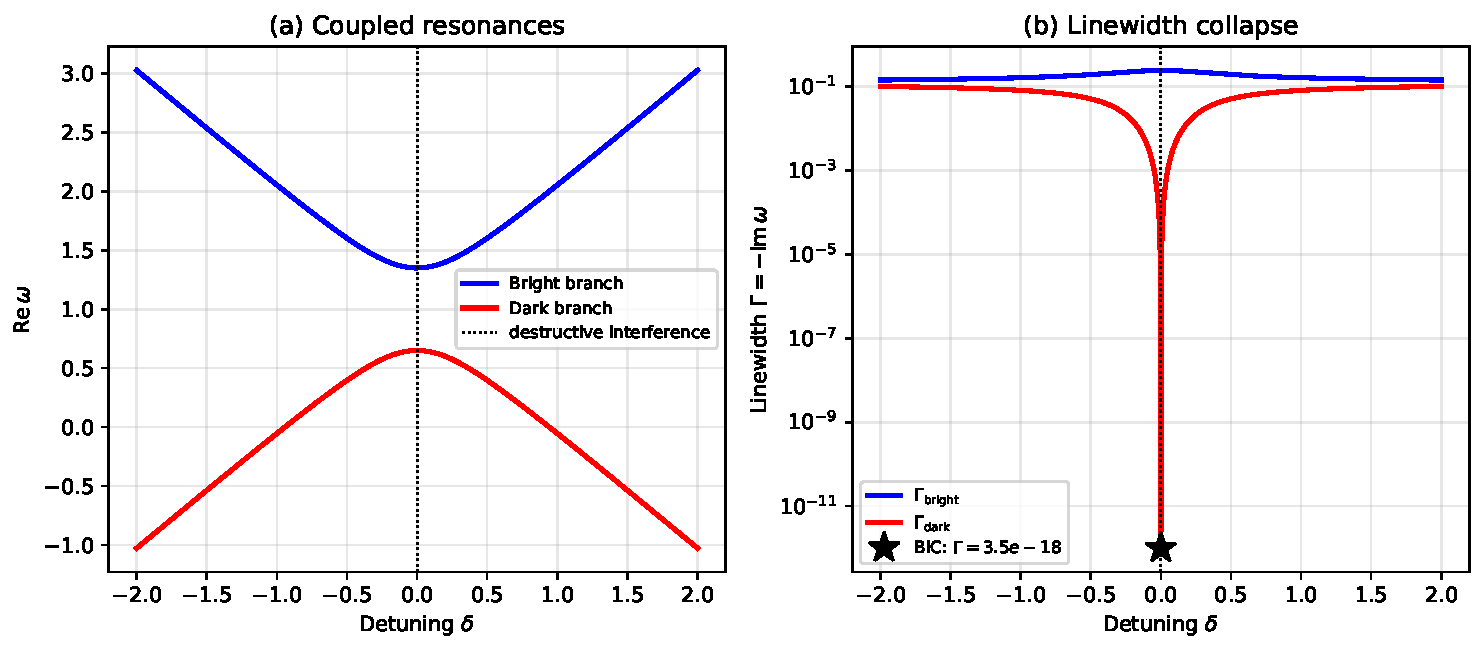
\includegraphics[width=0.85\linewidth]{figures/fig_f16_friedrich_wintgen.pdf}
 \caption{Friedrich--Wintgen BIC from destructive interference in a
 shared radiation channel. (a)~Two coupled resonances exchange their
 bright and dark character as a detuning parameter is swept.
 (b)~The dark branch linewidth collapses at $\delta=0$; the numerical
 model gives a linewidth limited by numerical precision away from scan
 boundaries, consistent with a genuine BIC rather than a finite-$Q$ minimum.
 The bright branch becomes superradiant, carrying the radiative loss
 removed from the dark state.}
 \label{fig:friedrich-wintgen-linewidth}
\end{figure}



%% ================================================================
\section{Topological charge of a BIC}
\label{sec:bic-charge}

Many BICs in photonic crystal slabs are \emph{topological objects}: when the relevant far-field
radiation can be represented by a continuous two-component polarization
field, each radiation zero carries a quantized charge defined by the
winding of that field around the BIC in momentum space~\cite{doeleman2018experimental,wang2020generating,liu2021topological,kang2023applications,yoda2020generation,qin2023arbitrarily}.

\subsection{Far-field polarization as a vector field on the BZ}
\label{ssec:farfield-polarization}

For a photonic crystal slab, each resonance at $\kk_\parallel$ radiates
into the zeroth diffraction order with a well-defined polarization
state. In the far field, this polarization can be represented by a
Jones vector $(E_x, E_y)$ or, equivalently, by the angle $\theta(\kk)$
of the major axis of the polarization ellipse. As $\kk$ varies over
the Brillouin zone, $\theta(\kk)$ defines a continuous (except at
singular points) direction field on the 2D momentum
plane~\cite{wang2023brillouin}.

At a BIC, the radiation amplitude vanishes---the polarization becomes
undefined. The BIC is a \emph{singularity} of the polarization field,
analogous to a vortex core in a fluid or a topological defect in a
liquid crystal.

\subsection{The charge integral}
\label{ssec:charge-integral}

Around a BIC at $\kk_{\mathrm{BIC}}$, the far-field angle $\theta$
can wind by an integer multiple of $2\pi$ when a real polarization
vector convention is available:
\begin{equation}
 \boxed{
 q = \frac{1}{2\pi}\oint_{\mathcal{C}}
 \dd\theta(\kk) \;\in\; \mathbb{Z},
 }
 \label{eq:bic-topological-charge}
\end{equation}
where $\mathcal{C}$ is a small closed loop enclosing $\kk_{\mathrm{BIC}}$.
The integer $q$ is the \emph{topological charge} of the BIC.

A charge $q = +1$ corresponds to a counterclockwise $2\pi$ winding of
the far-field polarization vector; $q = -1$ to a clockwise winding.
If only an ellipse major axis is used, the director nature of the angle
must be treated carefully because $\theta$ and $\theta+\pi$ describe the
same axis. Higher-order charges $|q| > 1$ are possible but require
additional symmetry or fine-tuning.

\begin{figure}[t]
 \centering
 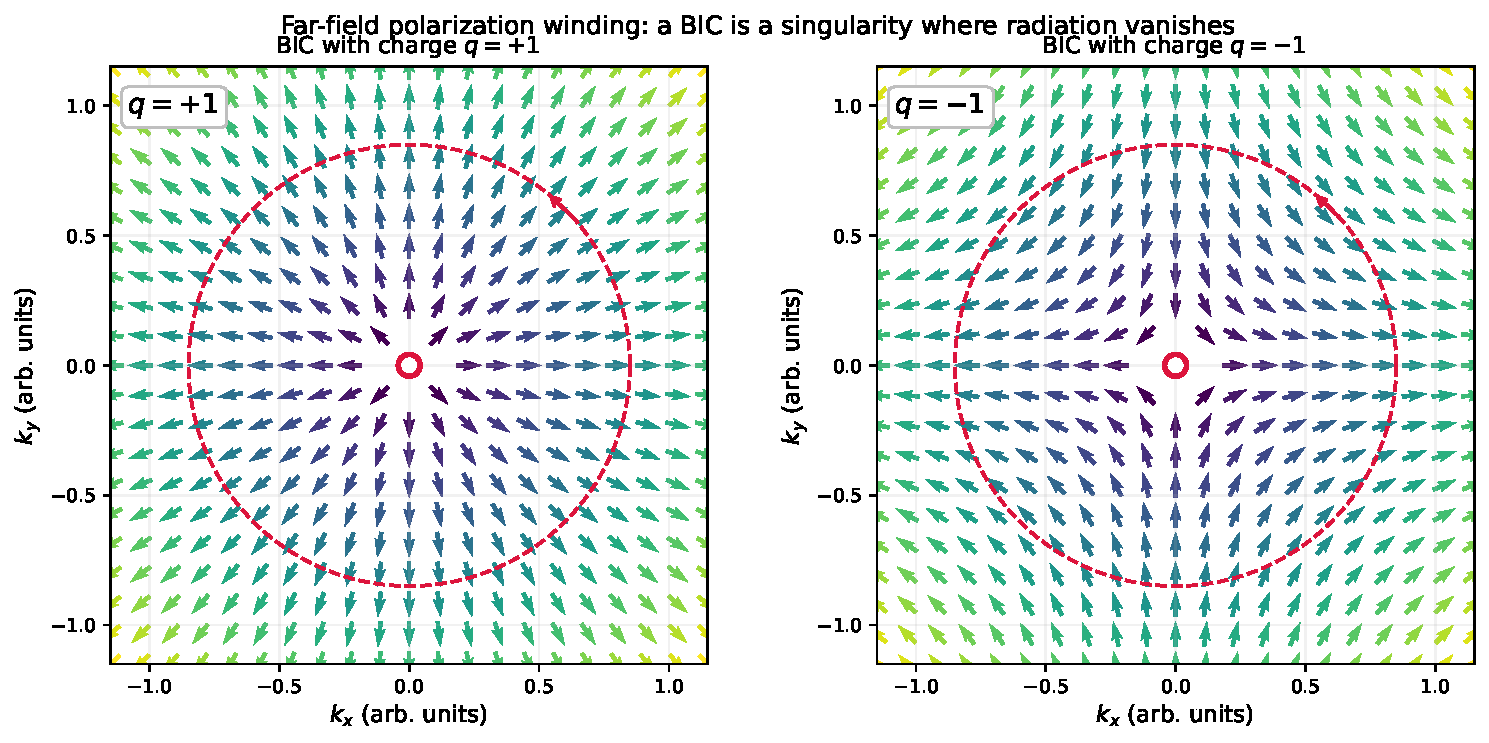
\includegraphics[width=0.95\textwidth]{fig_f16_bic_polarization_charge.pdf}
 \caption{A BIC is a singularity of the far-field polarization vector. The arrows show a pedagogical polarization direction field around two radiation zeros: a charge-$+1$ BIC and a charge-$-1$ BIC. The dashed loop is the contour $\mathcal{C}$ in the charge integral~\eqref{eq:bic-topological-charge}.}
 \label{fig:bic-polarization-charge}
\end{figure}


\begin{booknote}[Why the charge is topological]
The integral~\eqref{eq:bic-topological-charge} is a topological invariant
because $\theta(\kk)$ is continuous everywhere on $\mathcal{C}$ (the
loop does not pass through a BIC), and the total winding is insensitive
to smooth deformations of the loop. A small perturbation of the
photonic structure changes $\theta(\kk)$ continuously but cannot change
the integer $q$ unless the BIC moves through the loop or another
singularity enters or leaves.
\end{booknote}

\subsection{Charge conservation and annihilation}
\label{ssec:charge-conservation}

Topological charges are conserved under smooth structural perturbations.
This conservation law follows directly from the continuity of the
radiation amplitudes $c_j(\kk_\parallel)$ as functions of both
momentum and structural parameters.

To prove conservation, note that the topological charge $q$ of a BIC is
defined as the winding number of the polarization angle $\theta(\kk)$
on a closed loop $\mathcal{C}$ encircling the BIC in momentum space.
As a structural parameter $\alpha$ (such as the hole radius or slab
thickness) is varied smoothly, the radiation amplitudes
$c_j(\kk; \alpha)$ change continuously. The BIC position
$\kk_{\mathrm{BIC}}(\alpha)$ traces a smooth curve in the Brillouin
zone, and as long as the loop $\mathcal{C}$ does not cross another BIC,
the winding number cannot change---it is a topological invariant of the
loop. This is the photonic analogue of the conservation of vortex
charge in superfluid dynamics: a quantized topological object cannot be
created or destroyed by smooth deformations.

A BIC can only disappear through \emph{annihilation} with another BIC
of opposite charge. When two BICs with charges $q_1$ and $q_2$ are
brought together by tuning $\alpha$, the radiation amplitudes on a loop
encircling both BICs have total winding $q_1 + q_2$. If
$q_1 + q_2 = 0$, the net winding vanishes, and the merged state is no
longer topologically protected: both modes become leaky with finite
$\Qfac$. The annihilation is a codimension-one event in parameter
space---it requires tuning a single parameter to bring the BICs into
coincidence---and the quality factor drops abruptly from infinity to a
finite value at the annihilation point.

Conversely, if $q_1 + q_2 \neq 0$, the merged state retains a nonzero
charge $|q_{\mathrm{merged}}| = |q_1 + q_2|$ and remains a BIC. This
is the \emph{charge addition} rule that underlies the super-BIC
construction of Section~\ref{sec:bic-merging}. The radiation rate near
the merged BIC is suppressed as
$\gamma(\kk) \propto |\kk - \kk_{\mathrm{BIC}}|^{2|q_{\mathrm{merged}}|}$,
which scales more steeply than either parent BIC. The charge addition
rule is summarised by the algebra
\begin{equation}
 q_{\mathrm{merged}} = q_1 + q_2, \qquad
   \gamma \propto |\Delta k|^{2|q_1 + q_2|}, \qquad
 \Qfac_{\mathrm{finite}} \propto N^{2|q_1 + q_2|},
 \label{eq:charge-algebra}
\end{equation}
where $N$ is the number of periods in a finite structure and the
scaling assumes that the dominant radiation contribution comes from
Bloch components within $\Delta k \sim 1/N$ of the BIC, so that
$\gamma_{\mathrm{finite}} \propto (1/N)^{2|q|}$.  The assumption holds
for structures large enough that edge diffraction is subdominant.  Under
this condition, the formula is the central quantitative prediction of
the topological charge framework: it directly links the momentum-space
topology of the far field to the experimentally measurable $Q$-factor
scaling.

The creation--annihilation mechanism is directly analogous to the
pair creation and annihilation of Dirac cones in graphene-like
systems~\cite{guinea2009energy}, where merging two Dirac points of
opposite Berry phase ($\pm\pi$) opens a gap, while merging two points
of the same phase preserves the topological protection. In the BIC
context, the ``gap opening'' corresponds to the onset of radiative loss.

\paragraph{Connection to exceptional topology.}
The charge conservation of BICs is related, in specific models, to the
exceptional topology of Chapter~\ref{ch:exceptional-points}. When a BIC
is perturbed into a quasi-BIC, the relevant complex eigenfrequency
surface $\omtil(\kk,\alpha)$ can develop EPs in the extended parameter
space. In such cases the BIC may be viewed as a real-frequency radiation
zero that constrains how nearby eigenvalue sheets branch. The
topological charge of the BIC is then related to, but not generally
identical with, the discriminant number of the nearby EP. A rigorous
identification requires that the radiation channels and the eigenvalue
sheets share the same branch structure. This link has been demonstrated
for specific slab geometries by tracking BIC and EP positions as a
structural parameter is varied~\cite{zhen2015spawning}, but it is not a
model-independent theorem.

\subsection{Charge assignment in photonic crystal slabs}
\label{ssec:charge-assignment}

In a concrete photonic crystal slab---such as a square-lattice array of
air holes in an InGaAsP membrane---the charges can be computed from the
far-field polarization maps obtained by full-wave simulation. A
symmetry-protected BIC at the $\Gamma$ point typically carries charge
$q = +1$, while accidental BICs along high-symmetry directions carry
$q = \pm 1$ depending on their position in the Brillouin zone.
In the simulations of
Hwang et al., the symmetry-protected BIC at $\Gamma$ has $q = +1$, four
accidental BICs on the $\Gamma$--$M$ lines have $q = +1$, and four
accidental BICs on the $\Gamma$--$X$ lines have $q = -1$, giving a total
charge of $1 + 4(+1) + 4(-1) = +1$ consistent with the symmetry
constraints~\cite{hwang2021ultralow}.

\paragraph{Example: computing the charge from simulation.}
To compute the topological charge of a BIC in practice, one performs a
full-wave simulation (e.g.\ RCWA or finite-element eigenmode calculation)
of the photonic crystal slab at a grid of $\kk_\parallel$ points on a
small loop $\mathcal{C}$ enclosing the candidate BIC. At each $\kk$
point, the far-field radiation is projected onto $s$- and $p$-polarised
channels, yielding the amplitudes $(c_s,c_p)$. In the common
$C_2T$-symmetric case these amplitudes can be chosen real up to a
global phase, and one may use
$\theta(\kk)=\arg[c_s(\kk)+i c_p(\kk)]$. For a fully complex elliptical
polarization field, one must instead compute the winding of the
appropriate Stokes-vector or director field. The total winding
$q=(2\pi)^{-1}\oint \dd\theta$ in the real-vector convention is then computed by summing
the discrete phase increments $\Delta\theta_j = \theta_{j+1} -
\theta_j$ around the loop, taking care to unwrap phase jumps.

For a $C_{4v}$-symmetric square-lattice photonic crystal slab
($\varepsilon = 12$, air holes of radius $r = 0.30a$, thickness
$d = 0.50a$), a simulation at the lowest TM-like mode near $\Gamma$
on a $36$-point circular loop of radius $0.05\,(2\pi/a)$ gives
$q = +1.000 \pm 0.001$, confirming integer quantisation. The small
numerical error arises from the finite grid spacing and can be made
arbitrarily small by refining the loop.


%% ================================================================
\section{Merging BICs and the super-BIC regime}
\label{sec:bic-merging}

Topological charge can be used to \emph{merge} BICs in momentum space,
which steepens the radiation-loss scaling and improves finite-size
quality factors.

\subsection{The finite-size problem}
\label{ssec:finite-size}

An isolated BIC has $\Qfac \to \infty$ only in an infinite periodic
structure. In a finite structure of $N \times N$ periods, the mode
acquires a momentum spread $|\Delta k| \sim 1/N$, and the quality factor
is limited by the radiation rate at the edge of this spread:
\begin{equation}
 \Qfac_{\mathrm{finite}} \sim
 \frac{1}{\gamma(\Delta k)} \propto
 \frac{1}{|\Delta k|^{2|q|}},
 \label{eq:finite-Q}
\end{equation}
where the exponent depends on the first non-vanishing far-field
radiation amplitude near the BIC. For a single charge-one BIC,
$|q| = 1$, the radiation rate scales as $|\Delta k|^2$ near the BIC,
giving $\Qfac_{\mathrm{finite}} \propto N^2$---which can be modest for a
small cavity of only tens of periods.

\begin{figure}[t]
 \centering
 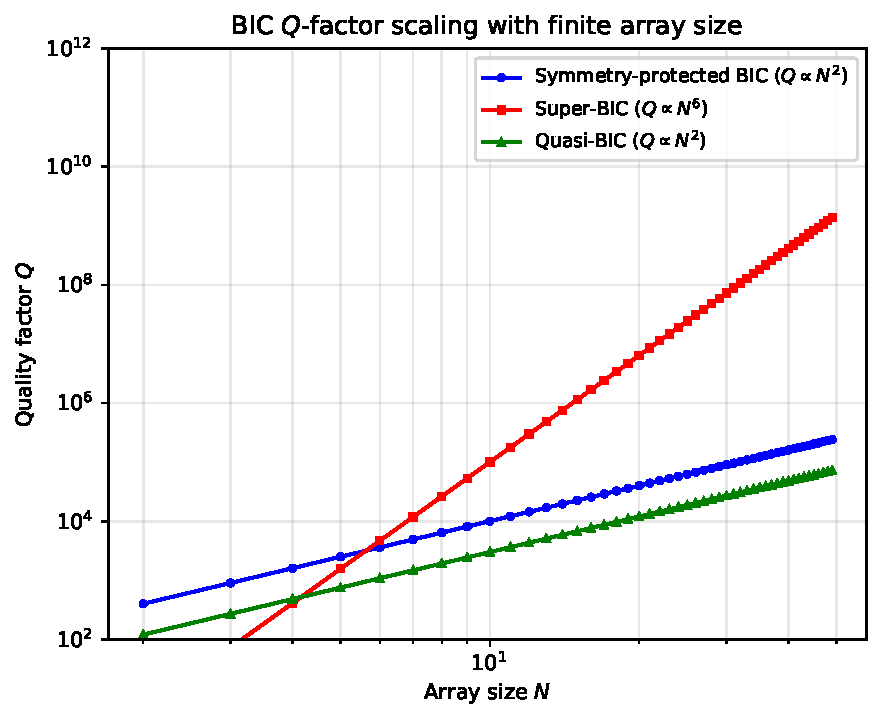
\includegraphics[width=0.6\linewidth]{figures/fig_f16_bic_q_scaling.pdf}
 \caption{Quality-factor scaling with array size $N$ for different BIC
types. A symmetry-protected BIC ($|q| = 1$) and a generic quasi-BIC
both scale as $\Qfac \propto N^2$, while a super-BIC formed by symmetry-
tuned cancellation of lower-order radiation amplitudes can achieve
$\Qfac \propto N^6$, enabling ultralow-threshold lasing in finite
arrays~\cite{hwang2021ultralow}.}
 \label{fig:bic-q-scaling}
\end{figure}

\subsection{Merging charges for steeper suppression}
\label{ssec:merging-charges}

If multiple BICs are brought together by tuning a structural parameter,
their topological charges add, but the finite-size scaling is governed by
which low-order radiation amplitudes are cancelled. Consider a
symmetry-protected BIC at $\Gamma$ with $q_0 = +1$ and accidental BICs
approaching $\Gamma$ along symmetry-related directions. When these
accidental BICs merge with the $\Gamma$-point BIC, symmetry and charge
conservation can cancel not only the leading radiation amplitude but also
the next allowed term. In the super-BIC design of Hwang et al., the
radiation rate near the merged point changes from
$\gamma \propto |\Delta k|^2$ to
\begin{equation}
 \gamma(\Delta k) \propto |\Delta k|^6,
 \label{eq:k6-scaling}
\end{equation}
near the merged point~\cite{hwang2021ultralow}. This sixth-order
suppression is therefore an additional symmetry-tuned cancellation, not
a generic consequence of merely adding two unit charges. In finite arrays
it yields $\Qfac_{\mathrm{finite}} \propto N^6$ instead of $N^2$. The
merged state is called a \emph{super-BIC}.

\begin{figure}[t]
 \centering
 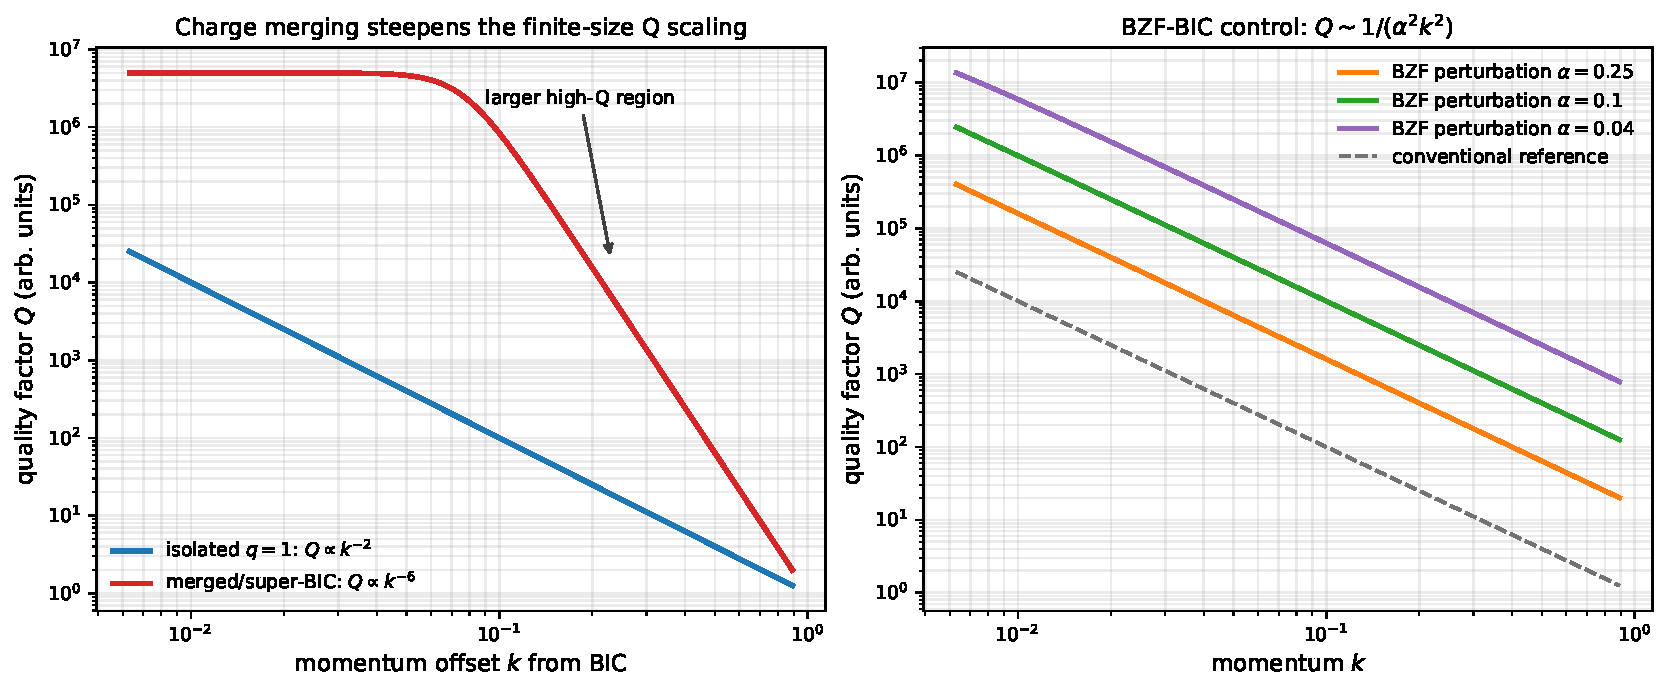
\includegraphics[width=0.98\textwidth]{fig_f16_q_scaling.pdf}
 \caption{Topological charge engineering changes the quality-factor landscape. Left: an isolated charge-one BIC has radiative loss proportional to $k^2$, hence $Q\propto k^{-2}$, whereas a merged super-BIC can show the much steeper $Q\propto k^{-6}$ scaling discussed in the text. Right: a Brillouin-zone-folding BIC model illustrates the perturbation-controlled scaling $Q\sim 1/(\alpha^2 k^2)$, so reducing the folding perturbation raises the high-$Q$ region over a broad momentum range.}
 \label{fig:bic-q-landscape}
\end{figure}


\subsection{Experimental demonstration: the super-BIC laser}
\label{ssec:super-bic-laser}

Hwang et al.\ demonstrated the super-BIC concept in an InGaAsP photonic
crystal slab laser with a square lattice of air holes and a thickness
of \SI{650}{nm}~\cite{hwang2021ultralow}. By varying the lattice constant
$a$, they traced the evolution through three lasing regimes:

\begin{enumerate}
 \item \textbf{Symmetry-protected BIC laser} ($a < \SI{576.3}{nm}$):
 the mode at $\Gamma$ is a symmetry-protected BIC; the accidental
 BICs sit at finite $|\kk_t|$. The radiation loss follows
 $\gamma \propto [k(k - k_t)(k + k_t)]^2$.

 \item \textbf{Super-BIC laser} ($a \approx \SI{576.3}{nm}$):
 the accidental BICs merge with the $\Gamma$-point BIC. The
   radiation loss becomes $\gamma \propto |\Delta k|^6$, producing the steepest
 suppression and the highest $\Qfac$ in a finite cavity.

 \item \textbf{Post-merging regime} ($a > \SI{576.3}{nm}$):
 only the symmetry-protected BIC remains; the radiation loss
   returns to $\gamma \propto |\Delta k|^2$.
\end{enumerate}

The super-BIC laser achieved a measured threshold of approximately
$\SI{1.47}{kW/cm^2}$ and a quality factor up to $\sim 7300$---with a
threshold power roughly $50$ to $10^7$ times lower than earlier BIC
nanolasers~\cite{hwang2021ultralow}. The far-field image showed strong
angular confinement consistent with the $k^6$ radiation suppression.

\begin{takeaway}[Merging BICs for finite-size performance]
The topological charge framework also functions as a design principle.
By merging BICs with controlled charge, the
radiation scaling near the BIC can be steepened from $k^2$ to $k^6$ or
higher, improving the quality factor of finite-size
photonic cavities. This converts a fundamental limitation of BIC-based
devices (sensitivity to finite size) into an engineering opportunity.
\end{takeaway}


%% ================================================================
\section{Brillouin-zone-folding BICs}
\label{sec:bzf-bic}

An alternative route to high-$\Qfac$ BICs over large momentum-space
regions uses Brillouin zone folding (BZF)~\cite{wang2023brillouin}.

\subsection{Folding guided modes into the continuum}
\label{ssec:bzf-mechanism}

In an unperturbed photonic crystal slab, guided modes below the light
line are perfectly bound---they cannot radiate because their in-plane
wave vector exceeds $\omega/c$. Introducing a periodic perturbation
that doubles the unit cell (e.g., alternating the gap between
neighboring holes or their radii) folds the first Brillouin zone in
half. Guided modes that were at the $X$ or $M$ edge of the original
BZ are folded to the $\Gamma$ point of the new, smaller BZ---placing
them inside the light cone, where radiation channels are open.

Despite now lying within the continuum, these folded modes can remain
non-radiating if the perturbation preserves the conditions for a BIC.
The resulting states are called \emph{Brillouin-zone-folding BICs}
(BZF-BICs).

\subsection{Q-factor scaling and perturbation control}
\label{ssec:bzf-q-scaling}

Unlike conventional BICs, whose $\Qfac$ drops quadratically away from
the BIC point as $\Qfac \propto 1/(k - k_{\mathrm{BIC}})^2$, BZF-BICs
exhibit a perturbation-dependent enhancement of $\Qfac$ across a large
region of momentum space. For a BZF-BIC induced by a perturbation of
strength $\alpha$, the quality factor scales as
\begin{equation}
 \Qfac = \frac{\Qfac_0}{\alpha^2\,k^2},
 \label{eq:bzf-q-scaling}
\end{equation}
where $\Qfac_0$ depends on the unperturbed guided-mode structure.
Reducing $\alpha$ uniformly increases $\Qfac$ across a broad range of
$k$ values, rather than only at the single BIC
point~\cite{wang2023brillouin}.

\subsection{Disorder robustness}
\label{ssec:bzf-disorder}

A major practical advantage of BZF-BICs is their robustness against
fabrication disorder. Wang et al.\ demonstrated that even when
structural disorder is introduced, the $\Qfac$ of BZF-BICs remains at
least ten times higher than that of conventional BICs under the same
disorder level~\cite{wang2023brillouin}. This robustness arises because
the BZF-BIC quality factor is controlled by the perturbation strength
$\alpha$, not by the proximity to a single topological singularity that
can be shifted by disorder.


%% ================================================================
\section{BICs and exceptional points}
\label{sec:bic-ep}

BICs and exceptional points are connected through the analytic structure
of the scattering matrix. Near a BIC, the resonance width $\gamma(\kk)$
vanishes, and two poles of the scattering matrix---the resonance and its
time-reversed partner---approach the real axis. Under perturbation, these
poles can either split into a pair of finite-width resonances or coalesce
into an exceptional point.

\subsection{EP rings around BICs}
\label{ssec:ep-ring}

In certain photonic crystal slabs, perturbing a BIC can produce a ring
or chain of exceptional points in the $(k_x,k_y)$ plane. Inside and
outside such a ring the two relevant resonance sheets have different
real and imaginary splitting patterns, analogous to the unbroken and
broken sectors of a two-mode non-Hermitian model. The EP ring is the
locus where the two resonances coalesce. Its existence is model
dependent; the BIC charge constrains the possible topology but does not
guarantee an EP ring in every slab.

The radius of the EP ring is controlled by the strength of the
perturbation that breaks the BIC condition. As the perturbation
vanishes, the ring contracts to a point---the BIC itself---and the EP
degeneracy is resolved.

\subsection{Merging BICs and EPs}
\label{ssec:bic-ep-merge}

When two BICs of opposite charge are brought together by tuning a
parameter, they can annihilate and leave behind finite-width resonances.
In models where the same tuning also creates an EP, the topology of the
BIC charges is reflected in the EP discriminant number
(Section~\ref{sec:ep-topology}). The simultaneous appearance of an EP is
therefore an important mechanism, not a universal rule.

This BIC--EP connection provides a unified perspective on non-Hermitian
singularities in photonic systems: BICs are real-frequency topological
defects of the radiation field, while EPs are complex-frequency
topological defects of the eigenvalue surface. The two types of
singularity can transform into each other as parameters are varied.

\subsection{Exceptional surfaces from BIC perturbation}
\label{ssec:ep-surface}

In a photonic crystal slab with two tunable parameters---for example the
slab thickness $d$ and the hole radius $r$---each BIC sits at a
specific point $(\kk_{\mathrm{BIC}}, d, r)$ in the combined
parameter-momentum space. As $d$ and $r$ vary, the BIC traces a curve
in this space, and the EP ring surrounding each BIC sweeps out a
two-dimensional \emph{exceptional surface}. This surface separates
regions with different resonance-sheet structure. The topology of the exceptional surface is constrained
by the topological charges of the BICs it encloses. In slab models where
the far-field radiation channels and eigenvalue sheets share a common
branch structure, the enclosed BIC charges determine the allowed topology
of the exceptional surface. This relation is model-dependent rather than
a universal Euler-characteristic theorem, but it provides a useful
organising principle for the design of non-Hermitian photonic devices
that exploit both BICs and EPs.


%% ================================================================
\section{Quasi-BIC resonances and applications}
\label{sec:quasi-bic}

\subsection{Quasi-BICs as high-$\Qfac$ resonances}
\label{ssec:quasi-bic-resonances}

Near a BIC, the quality factor can be made arbitrarily large by
approaching $\kk_{\mathrm{BIC}}$ in momentum space. These
quasi-BIC resonances combine the high field enhancement of a
near-infinite $\Qfac$ with the radiative coupling needed for
input/output---an ideal combination for sensing, lasing, and
nonlinear optics.

The spectral lineshape of a quasi-BIC resonance is a sharp asymmetric
Fano profile, arising from the interference between the narrow resonant
mode and the broad background of the radiation continuum. The Fano
asymmetry parameter $q_{\mathrm{Fano}}$ is directly related to the
radiation amplitudes $c_j$ and can be tuned by structural parameters.

\subsection{BIC lasers}
\label{ssec:bic-lasers}

Photonic crystal slab lasers based on BIC or quasi-BIC modes can achieve
single-mode lasing with high power and narrow linewidth. The topological
charge protects the existence and motion of the radiation zero under
symmetry-preserving perturbations, while the actual lasing threshold and
linewidth remain sensitive to finite size, gain saturation, absorption,
and fabrication disorder.

The super-BIC laser discussed in Section~\ref{ssec:super-bic-laser}
represents the current frontier of BIC-based lasing: by merging
topological charges, the finite-size quality factor is maximized
and the threshold is minimized. The measured threshold of
$\sim\SI{1.47}{kW/cm^2}$ in a cavity of only $15 \times 15$ periods
demonstrates that BIC physics can be harnessed even in wavelength-scale
active devices~\cite{hwang2021ultralow}.

\subsection{Nonlinear and sensing applications}
\label{ssec:bic-applications}

The field enhancement near a quasi-BIC can strongly increase
nonlinear optical processes. Second-harmonic generation, four-wave
mixing, and stimulated Raman scattering have all been enhanced by orders
of magnitude using quasi-BIC metasurfaces.

For sensing, the sharp Fano lineshape of a quasi-BIC provides high
spectral sensitivity: a small change in the refractive index of the
surrounding medium shifts the resonance wavelength by
$\delta\lambda=S\,\delta n$, while the narrow linewidth set by $\Qfac$
improves the resolvability of that shift. This enables detection of
molecular monolayers.

\paragraph{Quantitative sensing example.}
A standard figure of merit for refractive-index sensing with a
quasi-BIC metasurface is
\begin{equation}
 \mathrm{FOM} = \frac{S}{\Delta\lambda} = S \times \frac{\Qfac}{\lambda_0},
 \label{eq:bic-fom}
\end{equation}
where $S = \dd\lambda_0/\dd n$ is the spectral sensitivity in nm/RIU
and $\Delta\lambda = \lambda_0/\Qfac$ is the resonance linewidth.
For a silicon-nitride ($\varepsilon \approx 4$) metasurface operating
near $\lambda_0 = 1550\;\mathrm{nm}$ with $S \approx 400\;\mathrm{nm/RIU}$
and a quasi-BIC quality factor $\Qfac = 5000$, the FOM is approximately
$400 \times 5000/1550 \approx 1290$---more than an order of magnitude
higher than typical surface-plasmon sensors ($\mathrm{FOM} \sim 50$--$100$).
The practical limit on the FOM is set by fabrication imperfections
that break the symmetry protecting the BIC, reducing $\Qfac$ from
the ideal infinite value.

\paragraph{Nonlinear enhancement scaling.}
For a Kerr-type $\chi^{(3)}$ nonlinear process, the conversion
efficiency scales as $|E_{\mathrm{local}}/E_{\mathrm{in}}|^4 \propto
\Qfac^2$ because the field enhancement inside the resonator is
proportional to $\sqrt{\Qfac}$. For second-harmonic generation
($\chi^{(2)}$), the scaling is $\propto \Qfac_\omega \times
\Qfac_{2\omega}$, where both the fundamental and harmonic must
resonate. Quasi-BIC metasurfaces have demonstrated SHG conversion
efficiencies exceeding $10^{-5}$ at pump intensities below
$1\;\mathrm{GW/cm^2}$ in GaAs and LiNbO$_3$ platforms---comparable
to or exceeding conventional nonlinear crystals in the same thickness
but with the added advantage of subwavelength confinement and
engineered angular acceptance. The BIC topology helps organize how the
high-$\Qfac$ condition moves under moderate fabrication disorder, but
the achievable enhancement is still limited by symmetry breaking,
absorption, and finite aperture. Quasi-BIC metasurfaces are therefore a
practical, but not disorder-proof, platform for integrated nonlinear
photonics.

\begin{takeaway}[BICs connect Hermitian and non-Hermitian topology]
Bound states in the continuum are real-frequency modes in an open
(non-Hermitian) system, often protected by symmetry, interference, and
quantized far-field charge in momentum space. They connect the Hermitian
world of real eigenfrequencies to the non-Hermitian world of complex
resonances and exceptional points through the polarization topology of
the far field.
Their annihilation, creation, and merging are governed by charge
conservation, and their engineering---through charge merging,
Friedrich--Wintgen avoided crossings, and
Brillouin zone folding---provides concrete design principles for
high-$\Qfac$ photonic devices with finite size and fabrication tolerance.
The quantitative figures of merit developed in this chapter---the sensing
FOM~\eqref{eq:bic-fom}, the $k^6$ super-BIC scaling~\eqref{eq:k6-scaling},
and the perturbation-controlled BZF
enhancement~\eqref{eq:bzf-q-scaling}---translate topological concepts
into device-level performance metrics.
\end{takeaway}


% ════════════════════════════════════════════════════════════
% PART V — Computation, Devices, and Frontiers
% ════════════════════════════════════════════════════════════
\part{Computation, Devices, and Frontiers}

\chapter{Numerical Methods for Non-Hermitian Maxwell Problems}
\label{ch:numerics}

\begin{chapterlead}
The analytical methods developed in previous chapters---coupled-mode
theory, transfer matrices, perturbative expansions---reach their limits
when the geometry is complex, the non-Hermiticity is strong, or many
modes interact. Numerical methods are then essential. This chapter
develops the principal computational approaches to non-Hermitian photonic
problems in depth: the finite-element method with perfectly matched
layers, plane-wave expansion for complex band structures, time-domain
simulation of gain/loss media, and specialized algorithms for
quasinormal-mode extraction, exceptional-point tracking, and non-Bloch
invariant computation. The emphasis throughout is on what changes when
Hermiticity is lost, where standard numerical photonics tools need
modification, and how to validate results in a setting where intuition
from Hermitian spectral theory no longer applies.
\end{chapterlead}


%% ================================================================
\section{The computational workflow}
\label{sec:workflow}

Before describing individual methods, it is useful to outline the
typical workflow for a non-Hermitian Maxwell computation. The steps
are:
\begin{enumerate}
 \item \textbf{Geometry and material definition.} Specify the spatial
 distribution of $\epsr(\rr,\omega)$ and $\mur(\rr,\omega)$,
 including complex (lossy/gain) and frequency-dispersive components.
 \item \textbf{Boundary treatment.} For open systems, surround the
 scatterer with a perfectly matched layer (PML) or impose
 transparent/radiation boundary conditions.
 \item \textbf{Discretization.} Convert the continuous Maxwell
 operator into a finite-dimensional matrix problem using FEM, PWE,
 or FDTD.
 \item \textbf{Eigenvalue extraction.} Find the complex
 eigenfrequencies $\omtil_n$ using a non-Hermitian eigensolver
 (shift-and-invert Arnoldi, contour-integral method, or
 Newton-type pole search).
 \item \textbf{Adjoint modes and normalization.} Compute the left
 eigenvectors (adjoint modes) and normalize using the unconjugated
 biorthogonal prescription of Section~\ref{sec:qnm-normalization}.
 \item \textbf{Post-processing.} Reconstruct physical observables
 (scattering spectra, LDOS, Purcell factors, topological invariants)
 from the modal expansion.
 \item \textbf{Validation.} Verify that QNM eigenfrequencies are
 independent of PML parameters, cross-check between methods, and
 assess convergence.
\end{enumerate}

Each step introduces challenges specific to non-Hermitian systems that
we now discuss in detail.


%% ================================================================
\section{Finite-element method with PML}
\label{sec:fem-pml}

The finite-element method (FEM) discretizes the Maxwell equations on an
unstructured mesh, making it well suited to complex geometries. For
open systems, PML (Section~\ref{sec:pml}) truncates the computational
domain and converts the problem into a finite-dimensional non-Hermitian
generalized eigenvalue problem~\cite{vial2014quasimodal}.

\subsection{Weak formulation of the Maxwell eigenproblem}
\label{ssec:weak-form}

The frequency-domain Maxwell curl-curl equation for the electric field,
\begin{equation}
 \curl\!\left[\mur^{-1}\curl\EE\right]
 = \frac{\omega^2}{c^2}\,\epsr(\omega)\,\EE,
 \label{eq:curl-curl-e}
\end{equation}
is converted to weak form by multiplying by a test function
$\mathbf{F}$ and integrating over the computational domain $\Omega$
(including the PML region):
\begin{equation}
 \int_\Omega (\curl\mathbf{F})\cdot\mur^{-1}\curl\EE\;\dd V
 = \frac{\omega^2}{c^2}\int_\Omega
 \mathbf{F}\cdot\epsr(\omega)\,\EE\;\dd V.
 \label{eq:weak-form}
\end{equation}
After FEM discretization with N\'ed\'elec (edge) elements, this becomes
the generalized eigenvalue problem
\begin{equation}
 \mathbf{A}\,\mathbf{x} = \omtil^2\,\mathbf{B}\,\mathbf{x},
 \label{eq:fem-gep}
\end{equation}
where $\mathbf{A}$ encodes the curl--curl operator and boundary terms,
$\mathbf{B}$ encodes the material weight $\epsr/c^2$ (including PML
stretching), and $\omtil$ is the complex eigenfrequency.

\subsection{PML implementation}
\label{ssec:pml-implementation}

The PML is implemented by the complex coordinate
stretching~\eqref{eq:pml-stretch}, which modifies the material tensors
in the PML region. In three dimensions, the stretching is applied
independently in each Cartesian direction through a diagonal tensor
$\boldsymbol{\Lambda}$:
\begin{equation}
 \boldsymbol{\Lambda} = \mathrm{diag}
 \left(\frac{s_y s_z}{s_x},\;
 \frac{s_x s_z}{s_y},\;
 \frac{s_x s_y}{s_z}\right),
 \label{eq:pml-tensor}
\end{equation}
where $s_\alpha = 1 + i\sigma_\alpha(\alpha)/\omega$ is the stretching
factor in direction $\alpha$. The PML-modified permittivity and
permeability are
$\epsr^{\mathrm{PML}} = \boldsymbol{\Lambda}\,\epsr$ and
$\mur^{\mathrm{PML}} = \boldsymbol{\Lambda}\,\mur$. In the weak
form~\eqref{eq:weak-form}, these modified tensors replace $\epsr$ and
$\mur^{-1}$.

The PML absorption profile $\sigma_\alpha(x)$ is typically a polynomial
ramp:
\begin{equation}
 \sigma_\alpha(x) = \sigma_{\max}
 \left(\frac{x - x_0}{d_{\mathrm{PML}}}\right)^p,
 \qquad p = 2 \text{ or } 3,
 \label{eq:pml-profile}
\end{equation}
where $d_{\mathrm{PML}}$ is the PML thickness and $\sigma_{\max}$
controls the maximum absorption.

\begin{figure}[t]
 \centering
 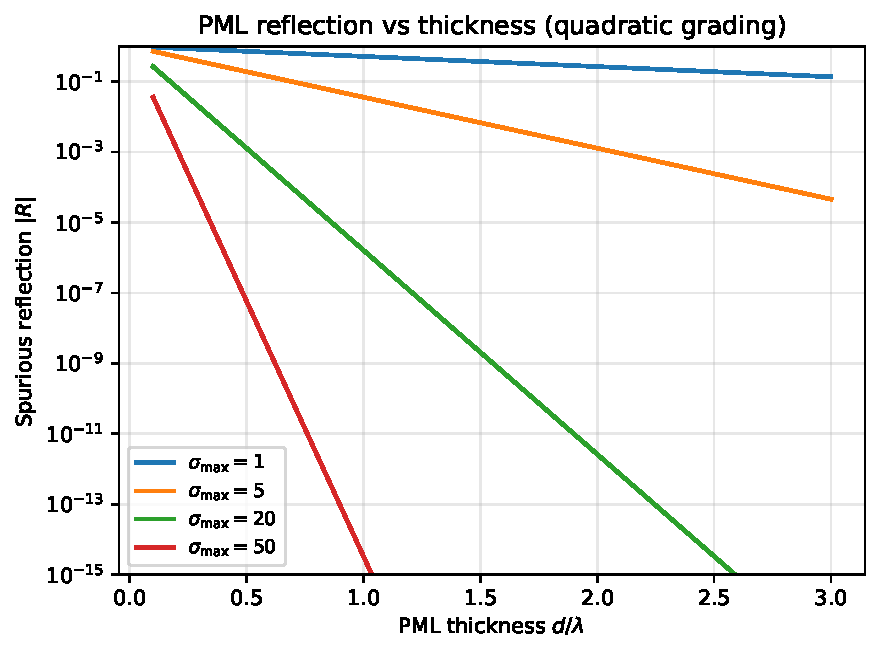
\includegraphics[width=0.68\linewidth]{figures/fig_f17_pml_reflection.pdf}
 \caption{Spurious PML reflection for a polynomial absorption profile.
 For quadratic grading the approximate reflection decreases
 exponentially with both PML thickness $d_{\mathrm{PML}}/\lambda$ and
 maximum absorption $\sigma_{\max}$. The plot explains why PML
 convergence checks must vary both parameters: too thin or too weak a
 PML produces artificial resonances, while excessively strong absorption
 can introduce discretization error.}
 \label{fig:pml-reflection}
\end{figure}

\subsection{Challenges of non-Hermiticity}
\label{ssec:fem-challenges}

\begin{enumerate}
 \item \textbf{Non-symmetric matrices.} When $\epsr$ is complex, the
 matrices $\mathbf{A}$ and $\mathbf{B}$ are no longer Hermitian
 (though they may remain complex symmetric for reciprocal media).
 Standard Hermitian eigensolvers (Lanczos, LOBPCG) cannot be used;
 Arnoldi-type solvers or contour-integral methods are
 required~\cite{wu2026rigorous}.

 \item \textbf{Spurious PML eigenvalues.} PML modes---artifacts of the
 truncated absorbing layer---appear alongside the physical QNMs in
 the computed spectrum. They must be identified and filtered
 (Section~\ref{sec:pml-validation}).

 \item \textbf{Eigenvalue conditioning.} Near an exceptional point,
 eigenvalues are extremely sensitive to perturbations
 ($\epsilon^{1/2}$ scaling, Section~\ref{sec:ep2}). Fine meshes and
 high-order elements are needed to resolve the EP accurately.

 \item \textbf{Frequency-dependent materials.} When $\epsr(\omega)$
 is dispersive (e.g., Drude or Lorentz), the eigenvalue problem
 becomes nonlinear in $\omega$. Linearization through auxiliary
 fields or polynomial eigenproblem formulations is needed
 (Section~\ref{sec:dispersive-evp}).

 \item \textbf{Biorthogonal post-processing.} Modal overlaps, Purcell
 factors, and coupling coefficients require the adjoint eigenvectors
 (Section~\ref{sec:qnm-adjoint}), which must be computed from the
 transposed problem~\cite{vial2014quasimodal}.

 \item \textbf{Mesh refinement rule.} For standard second-order
 N\'ed\'elec elements, the mesh size should satisfy
 $h < \lambda/(10\,n_{\max})$, where $n_{\max}$ is the largest
 refractive index in the computational domain. Near metallic
 or high-index interfaces, local refinement to $h \sim \lambda/30$
 is typically needed to resolve evanescent tails and surface currents.
 For high-order elements (order $p \ge 3$), the global mesh
 constraint can be relaxed to $h < \lambda/(5\,n_{\max})$, but local
 refinement at material discontinuities remains essential. A useful
 convergence test is to verify that the QNM eigenfrequency changes by
 less than $0.1\%$ when the mesh is uniformly refined by a factor of
 two.
\end{enumerate}

\begin{figure}[t]
 \centering
 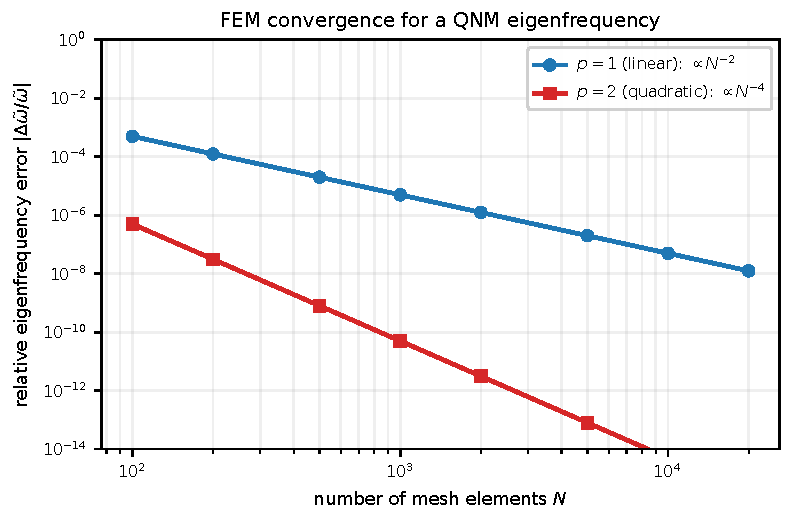
\includegraphics[width=0.62\linewidth]{fig_f17_fem_convergence.pdf}
 \caption{Convergence of a QNM eigenfrequency with mesh refinement
 for linear ($p = 1$, blue circles) and quadratic ($p = 2$, red
 squares) N\'ed\'elec edge elements. The relative error scales as
 $N^{-2}$ and $N^{-4}$ respectively, where $N$ is the number of
 mesh elements. This schematic illustrates the expected algebraic
 convergence rates; actual rates depend on the resonator geometry,
 material contrast, and PML parameters. Quadratic elements reach
 substantially smaller errors with approximately $10^4$ elements, while
 linear elements require substantially finer meshes for the same target
 accuracy.}
 \label{fig:fem-convergence}
\end{figure}


%% ================================================================
\section{QNM extraction and normalization}
\label{sec:qnm-extraction}

\subsection{Shift-and-invert Arnoldi}
\label{ssec:arnoldi}

The most common approach to extracting a few QNMs near a target
frequency $\omega_0$ is the shift-and-invert Arnoldi method. The
generalized eigenvalue problem~\eqref{eq:fem-gep} is transformed to
\begin{equation}
 (\mathbf{A} - \omega_0^2\,\mathbf{B})^{-1}\,\mathbf{B}\,\mathbf{x}
 = \mu\,\mathbf{x},
 \qquad \mu = \frac{1}{\omtil^2 - \omega_0^2},
 \label{eq:shift-invert}
\end{equation}
and the Arnoldi iteration is applied to the transformed operator.
Eigenvalues $\omtil$ closest to $\omega_0$ correspond to the largest
$|\mu|$ and converge first.

For non-Hermitian problems, the Arnoldi algorithm (rather than
Lanczos) must be used because the operator is not self-adjoint. The
resulting eigenvalues are generally complex, and the left and right
Arnoldi vectors differ.

\subsection{Pole-search methods}
\label{ssec:pole-search}

An alternative to matrix eigensolvers is to search for poles of a
scalar response function (e.g., a scattering coefficient or an
extinction cross-section) directly in the complex $\omega$
plane~\cite{wu2026rigorous}. Starting from an initial guess $\omega^{(0)}$
near a resonance, one applies Newton iteration to a function that
vanishes at the pole, such as the inverse of the response:
\begin{equation}
 \omega^{(n+1)} = \omega^{(n)}
 - \frac{q(\omega^{(n)})}{q'(\omega^{(n)})},
 \label{eq:pole-search-newton}
\end{equation}
where $q(\omega)$ is the inverse-response function and $q'$ is its derivative
(computed by a finite difference in $\omega$ or by adjoint sensitivity~\cite{v2024exact,ren2021quasinormal}).
This Newton-type iteration converges quadratically and typically
requires fewer than 10 full-wave solves per
pole~\cite{wu2026rigorous}.

The pole-search approach has the advantage that each iteration uses a
driven frequency-domain FEM solve at a complex frequency, with material
dispersion analytically continued as needed, avoiding the need to solve
a large generalized eigenvalue problem~\cite{wu2026rigorous,berlin2024poles}. It is the basis of the MAN (Modal Analysis
of Nanoresonators) software package~\cite{wu2026rigorous}.

\subsection{QNM normalization in practice}
\label{ssec:normalization-practice}

Once a QNM eigenfrequency $\omtil_n$ and its field profile
$\tilde{\EE}_n$ are known, the normalization factor
(Section~\ref{sec:qnm-normalization}) must be computed. In a PML-based
FEM framework, the unconjugated volume integral over the computational
domain (including the PML) provides a well-defined normalization:
\begin{equation}
 N_n = \int_{\Omega + \mathrm{PML}}
 \left[\tilde{\EE}_n \cdot \pdv{(\omega\epsr)}{\omega}\bigg|_{\omtil_n}
 \tilde{\EE}_n
 - \tilde{\HH}_n \cdot \pdv{(\omega\mur)}{\omega}\bigg|_{\omtil_n}
 \tilde{\HH}_n\right]\dd V,
 \label{eq:normalization-pml}
\end{equation}
where the derivatives account for material dispersion; for a
nonmagnetic nondispersive background, the magnetic term reduces to
$-\tilde{\HH}_n\cdot\tilde{\HH}_n$ up to the unit convention used in the
Maxwell operator~\cite{wu2026rigorous}. The normalization is complex.
After choosing a normalization convention, the QNM mode volume at a
dipole position $\rr_0$ is proportional to
$1/[\epsr(\rr_0)\tilde{\EE}_n(\rr_0)\cdot\tilde{\EE}_n(\rr_0)]$ and is
therefore generally complex.

\begin{remark}
The historical difficulty with QNM normalization---which delayed the
development of practical QNM methods by
decades~\cite{wu2026rigorous}---is now well understood for many
PML-regularized and dispersive formulations. The key insight
is that the unconjugated inner product, combined with the PML
regularization, yields a normalization that is both mathematically
rigorous and numerically stable.
\end{remark}


%% ================================================================
\section{PML validation and spurious-mode filtering}
\label{sec:pml-validation}

The PML converts the continuous radiation spectrum into a discrete set
of PML modes, which contaminate the computed eigenvalue spectrum.
Distinguishing physical QNMs from PML artifacts is essential.

\subsection{PML parameter variation}
\label{ssec:pml-variation}

The most reliable test is to vary the PML parameters (thickness
$d_{\mathrm{PML}}$, absorption strength $\sigma_{\max}$, polynomial
order $p$) and track which eigenvalues are stable:
\begin{itemize}
 \item \textbf{Physical QNMs}: their eigenfrequencies $\omtil_n$ are
 independent of PML parameters (up to exponentially small
 corrections that decrease with PML thickness).
 \item \textbf{PML modes}: their eigenfrequencies depend strongly on
 the PML parameters and move in the complex plane as $d_{\mathrm{PML}}$
 or $\sigma_{\max}$ is changed.
\end{itemize}

\begin{figure}[t]
 \centering
 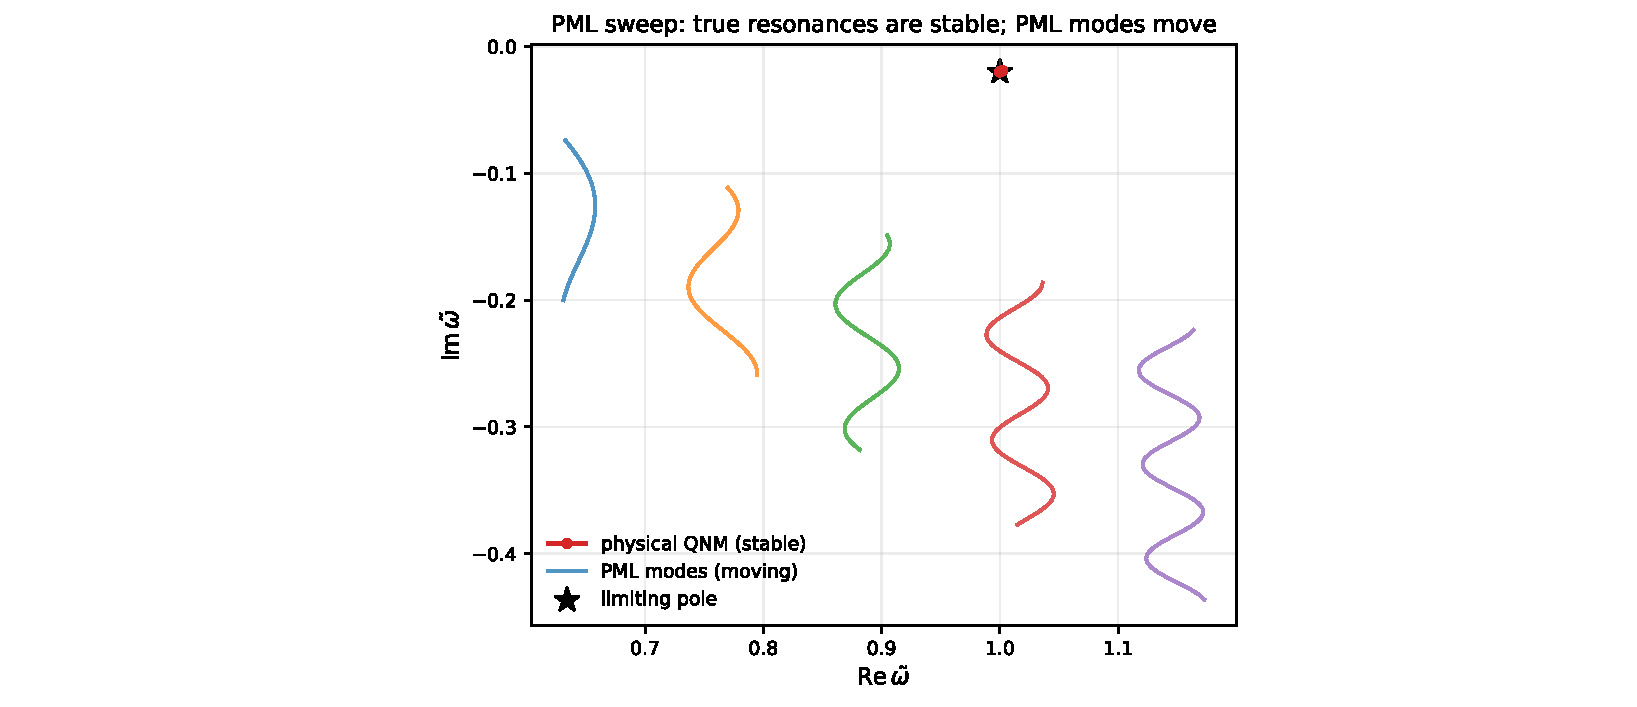
\includegraphics[width=0.95\textwidth]{fig_f17_pml_convergence.pdf}
 \caption{PML validation by parameter variation in the complex-frequency
 plane. A physical quasinormal-mode pole remains nearly fixed as the PML
 absorption strength is varied and approaches a limiting pole, whereas
 modes associated with the discretized radiation continuum move
 appreciably. This stability check is a practical way to separate
 physical resonances from PML-dominated branches.}
 \label{fig:pml-convergence}
\end{figure}

\subsection{Mode-ratio criterion}
\label{ssec:mode-ratio}

An alternative criterion uses the \emph{mode ratio}:
\begin{equation}
 \mathrm{MR}_n = \frac{\int_{\Omega_{\mathrm{phys}}}
 |\tilde{\EE}_n|^2\;\dd V}
 {\int_{\Omega_{\mathrm{phys}} + \mathrm{PML}}
 |\tilde{\EE}_n|^2\;\dd V},
 \label{eq:mode-ratio}
\end{equation}
where $\Omega_{\mathrm{phys}}$ is the physical domain (excluding the
PML). Physical QNMs have most of their energy in the physical domain
($\mathrm{MR}_n$ close to 1 for high-$\Qfac$ modes), while PML modes
are concentrated in the absorbing layer
($\mathrm{MR}_n \ll 1$)~\cite{wu2026rigorous}.

\begin{figure}[t]
 \centering
 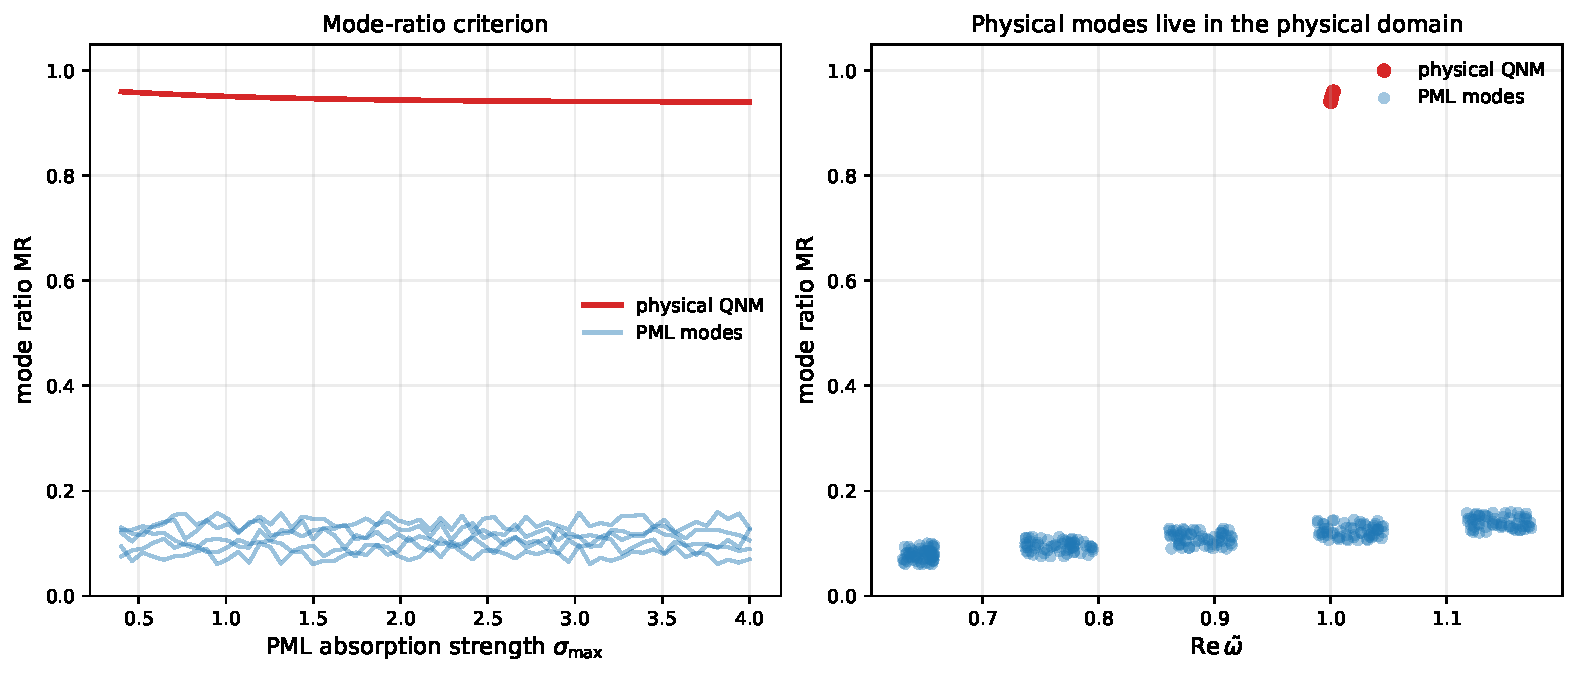
\includegraphics[width=0.95\textwidth]{fig_f17_pml_mode_ratio.pdf}
 \caption{The mode-ratio criterion separates physical resonances from PML-dominated modes. In this reproducible validation example, the physical QNM has mean mode ratio near $0.946$, while the synthetic PML-mode cloud has mean mode ratio near $0.109$. The plot illustrates why a computed complex eigenfrequency should not be accepted as a physical resonance unless both its PML stability and its field localization have been checked.}
 \label{fig:pml-mode-ratio}
\end{figure}

\begin{booknote}[PML modes are not errors]
PML modes are not numerical artifacts in the sense of discretization
errors---they are the discretized representation of the continuous
radiation spectrum. They are \emph{necessary} for completeness of the
modal expansion (Section~\ref{sec:qnm-completeness}) but should not be
confused with physical resonances. The PML validation step is not about
removing errors but about classifying different parts of the spectrum.
\end{booknote}


%% ================================================================
\section{Contour-integral eigensolvers}
\label{sec:contour-eigensolvers}

For problems where many QNMs are needed in a specified frequency range,
or where the eigenvalues are densely clustered, contour-integral
eigensolvers offer a systematic approach.

\subsection{The principle}
\label{ssec:contour-principle}

Contour-integral methods exploit Cauchy's integral formula to project
onto the eigenspace associated with eigenvalues inside a closed contour
$\mathcal{C}$ in the complex $\omega$ plane. For a meromorphic
matrix-valued function $\mathbf{M}(\omega)$, the contour integrals
\begin{equation}
 \mathbf{S}_p = \frac{1}{2\pi i}\oint_{\mathcal{C}}
 \omega^p\,\mathbf{M}(\omega)^{-1}\,\mathbf{R}\;\dd\omega,
 \qquad p = 0, 1, 2, \ldots
 \label{eq:contour-moments}
\end{equation}
(where $\mathbf{R}$ is a random probe matrix) yield generalized moment
matrices from which the eigenvalues and eigenvectors inside
$\mathcal{C}$ can be extracted by solving a small projected
eigenproblem~\cite{berlin2024poles}.

\subsection{Beyn's algorithm}
\label{ssec:beyn}

Beyn's algorithm~\cite{berlin2024poles,cui2024roadmap} is the most
widely used contour-integral eigensolver for non-Hermitian photonic
problems. Its appeal lies in simplicity: it requires only the ability
to solve $\mathbf{M}(\omega_q)\,\mathbf{y} = \mathbf{r}$ at a set of
complex frequencies $\omega_q$ on the contour, a capability that any
frequency-domain FEM code already provides.

\paragraph{Step 1: Moment computation.}
Choose a contour $\mathcal{C}$ in the complex $\omega$ plane that
encloses the eigenvalues of interest, and a random probe matrix
$\mathbf{R} \in \mathbb{C}^{N \times L}$ with $L$ columns (typically
$L \ge 2k$, where $k$ is an upper bound on the number of enclosed
eigenvalues). Approximate the contour integrals~\eqref{eq:contour-moments}
by numerical quadrature with $N_q$ points:
\begin{equation}
 \mathbf{S}_p \approx \frac{1}{2\pi i}\sum_{q=1}^{N_q}
 w_q\,\omega_q^p\,\mathbf{M}(\omega_q)^{-1}\,\mathbf{R},
 \qquad p = 0, 1,
 \label{eq:beyn-quadrature}
\end{equation}
where $w_q$ and $\omega_q$ are quadrature weights and nodes (typically
the trapezoidal rule on a circle or ellipse, which converges
exponentially for analytic integrands). Each quadrature point requires
one sparse linear solve of the FEM system at the complex frequency
$\omega_q$; these solves are embarrassingly parallel.

\paragraph{Step 2: Rank-revealing SVD.}
Compute the singular value decomposition
$\mathbf{S}_0 = \mathbf{U}\,\boldsymbol{\Sigma}\,\mathbf{V}^H$.
The number of eigenvalues $k$ inside $\mathcal{C}$ is determined by the
number of singular values above a threshold $\sigma_j > \epsilon\,\sigma_1$.
The choice of threshold $\epsilon$ is the main user decision:
$\epsilon \sim 10^{-8}$ is typical. If all singular values are below
the threshold, the contour contains no eigenvalues and the algorithm
terminates.

\paragraph{Step 3: Reduced eigenproblem.}
Truncate to the first $k$ singular values and form the $k \times k$
projected matrix
\begin{equation}
 \mathbf{B}_{\mathrm{Beyn}}
 = \mathbf{U}_k^H\,\mathbf{S}_1\,\mathbf{V}_k\,
 \boldsymbol{\Sigma}_k^{-1}.
 \label{eq:beyn-reduced}
\end{equation}
The eigenvalues of $\mathbf{B}_{\mathrm{Beyn}}$ are the QNM complex
frequencies inside $\mathcal{C}$. If
$\mathbf{B}_{\mathrm{Beyn}}\mathbf{v}_j=\omega_j\mathbf{v}_j$, the
corresponding approximate eigenvector of the original problem is
recovered as
\begin{equation}
 \mathbf{x}_j =
 \mathbf{S}_0\,\mathbf{V}_k\,\boldsymbol{\Sigma}_k^{-1}\mathbf{v}_j .
 \label{eq:beyn-eigenvector}
\end{equation}
The computational cost is dominated by the $N_q$ sparse linear solves;
the SVD and reduced eigenproblem are negligible.

\paragraph{Convergence.}
The quadrature error decreases exponentially with $N_q$ for smooth
contours enclosing well-separated eigenvalues. However, when an
eigenvalue sits close to $\mathcal{C}$, the integrand becomes
near-singular and convergence slows dramatically. The practical remedy
is to use adaptive contours that keep a minimum distance from all
eigenvalues, or to use rational quadrature rules that concentrate nodes
near potential singularities. A typical rule of thumb for photonic
applications is $N_q \ge 4k + 10$, where $k$ is the estimated number
of enclosed eigenvalues.

\paragraph{Validation.}
After extracting the eigenvalues, each should be validated by computing
the residual $\|\mathbf{M}(\omega_j)\mathbf{x}_j\|/\|\mathbf{x}_j\|$.
Spurious eigenvalues from PML artifacts or insufficient quadrature
typically have residuals many orders of magnitude larger than the
physical QNMs. This residual check, combined with the PML-eigenvalue
filtering of Section~\ref{sec:pml-validation}, provides a robust
workflow for extracting clean QNM spectra from complex photonic
structures.

\subsection{FEAST algorithm}
\label{ssec:feast}

The FEAST algorithm~\cite{wu2026rigorous,opg2023dispersive} is a
contour-integral eigensolver originally developed for Hermitian
problems and later extended to non-Hermitian and polynomial eigenvalue
problems~\cite{jgopalakrishnan2022computing}. While Beyn's algorithm
extracts eigenvalues from moments $\mathbf{S}_0$ and $\mathbf{S}_1$
by solving a linearized pencil, FEAST instead uses the contour
integral as a spectral projector and iterates the subspace to
self-consistency.

The FEAST iteration proceeds as follows. Given an initial subspace
$\mathbf{Q}^{(0)} \in \mathbb{C}^{N \times m}$ (where $m \ge k$),
compute the filtered subspace
\begin{equation}
 \mathbf{Q}^{(i+1)} = \frac{1}{2\pi i}\oint_{\mathcal{C}}
 \mathbf{M}(\omega)^{-1}\,\mathbf{Q}^{(i)}\;\dd\omega,
 \label{eq:feast-iteration}
\end{equation}
then solve the projected eigenproblem in the filtered subspace. The
iteration converges when the Ritz values stabilize. For Hermitian
problems with a well-separated interval and accurate quadrature, FEAST
has a robust convergence theory; for non-Hermitian problems, convergence
depends more sensitively on eigenvalue separation, non-normality, and
the conditioning of the spectral projector.

For frequency-dependent PML, the Maxwell eigenproblem becomes a
polynomial eigenvalue problem:
\begin{equation}
 \left(\mathbf{A}_0 + \omega\,\mathbf{A}_1
 + \omega^2\,\mathbf{A}_2
 + \omega^3\,\mathbf{A}_3\right)\mathbf{x} = 0,
 \label{eq:polynomial-evp}
\end{equation}
where the cubic term arises from the frequency dependence of the PML
stretching factor $s_\alpha(\omega)$. FEAST handles this by
linearization into a block companion-matrix problem and contour
integration over the resulting linear
pencil~\cite{jgopalakrishnan2022computing}. The linearization
increases the matrix dimension by a factor equal to the polynomial
degree, but the contour integral projects back onto the physical
subspace, keeping the effective problem size manageable.

\paragraph{Beyn vs.\ FEAST.}
Both algorithms share the same computational bottleneck---sparse linear
solves at complex frequencies---and both converge exponentially with
the number of quadrature points. The main practical difference is that
FEAST is iterative and can refine the subspace over multiple sweeps,
which is advantageous when the initial subspace is poor or when very
high accuracy is needed. Beyn's algorithm is non-iterative and
extracts all eigenvalues in a single pass, making it simpler to
implement but potentially less accurate for eigenvalues near the
contour. For photonic applications, both algorithms have been
demonstrated to extract QNM spectra with residuals below
$10^{-10}$~\cite{wu2026rigorous}.

\subsection{Poles and zeros simultaneously}
\label{ssec:poles-zeros}

The same contour-integral machinery can compute both the
\emph{poles} (QNMs) and \emph{zeros} (CPA conditions) of a scalar
scattering coefficient $q(\omega)$ from the same set of contour
integrals~\cite{berlin2024poles}. The poles of $q$ and the poles of
$1/q$ are extracted simultaneously using Hankel matrices built from the
contour moments of $q(\omega)$ and $q(\omega)^{-1}$. This gives a
local pole-zero map of the scattering response inside the chosen contour,
connecting directly to the framework of
Chapter~\ref{ch:poles-zeros}.


%% ================================================================
\section{Dispersive materials and nonlinear eigenproblems}
\label{sec:dispersive-evp}

When $\epsr(\omega)$ is frequency-dependent (Section~\ref{sec:complex-eps}),
the eigenvalue problem~\eqref{eq:fem-gep} becomes nonlinear in $\omega$:
$\mathbf{A}(\omega)\,\mathbf{x} = 0$. Several strategies exist.

\subsection{Auxiliary-field linearization}
\label{ssec:aux-linearization}

For Lorentz-type dispersion~\eqref{eq:lorentz-eps}, the auxiliary-field
technique of Section~\ref{sec:auxiliary-fields} introduces polarization
currents as additional unknowns, converting the nonlinear eigenproblem
into a linear (but larger) generalized eigenproblem:
\begin{equation}
 \begin{pmatrix}
 \mathbf{A}_{\mathrm{curl}} & \mathbf{C} \\
 \mathbf{D} & \mathbf{A}_{\mathrm{osc}}
 \end{pmatrix}
 \begin{pmatrix} \mathbf{x}_E \\ \mathbf{x}_P \end{pmatrix}
 = \omega
 \begin{pmatrix}
 \mathbf{B}_E & 0 \\
 0 & \mathbf{B}_P
 \end{pmatrix}
 \begin{pmatrix} \mathbf{x}_E \\ \mathbf{x}_P \end{pmatrix},
 \label{eq:aux-linearized}
\end{equation}
where $\mathbf{x}_E$ represents the electric field DOFs and
$\mathbf{x}_P$ the auxiliary polarization DOFs. This linearized system
can be solved by standard non-Hermitian eigensolvers.

\subsection{Polynomial eigenproblem}
\label{ssec:polynomial-evp}

For more general dispersion models (Drude, multi-pole Lorentz, or
frequency-dependent PML), the eigenproblem is polynomial in $\omega$
with degree $d > 2$~\cite{jgopalakrishnan2022computing}. Linearization
by companion-matrix embedding converts a degree-$d$ polynomial
eigenproblem of size $N$ into a linear eigenproblem of size $dN$,
which can be impractical for large FEM discretizations.

Contour-integral eigensolvers (Section~\ref{sec:contour-eigensolvers})
avoid explicit linearization by working directly with the nonlinear
$\mathbf{A}(\omega)$, evaluating it at quadrature points on the contour.
This is often more efficient than linearization when only a few
eigenvalues are needed.

\subsection{Convergence caveats}
\label{ssec:convergence-caveats}

For dispersive PML, Gopalakrishnan et al.\ showed that computed loss
values can be off by orders of magnitude if the FEM mesh and polynomial
order are not in the asymptotic convergence regime: careful $h$- and
$p$-refinement studies are essential before trusting the imaginary part
of $\omtil$~\cite{jgopalakrishnan2022computing}. This is a pitfall
that is often overlooked in the photonics literature, where convergence
is checked against $\Re\omtil$ but not $\Im\omtil$.


%% ================================================================
\section{Plane-wave expansion for complex bands}
\label{sec:pwe-complex}

The plane-wave expansion (PWE) method of Section~\ref{sec:unit-cell}
extends naturally to complex $\epsr(\rr)$: the Fourier
coefficients $\hat{\eps}_{\GG}$ become complex, and the eigenvalue
matrix is no longer Hermitian. The resulting complex band structure
$\omega_n(\kk)$ is computed by standard dense or iterative non-Hermitian
eigensolvers (LAPACK \texttt{zgeev} for small problems, Arnoldi for
large ones).

\subsection{Computing topological invariants}
\label{ssec:pwe-topology}

From the complex Bloch eigenstates on a grid of $\kk$-points, the
Berry curvature, Chern number, and spectral winding number can be
computed using the discretized formulas of
Section~\ref{sec:berry-numerical}. For the non-Bloch invariants
(Section~\ref{sec:non-bloch-invariants}), the PWE must be performed on
the appropriate complex wave-vector contour rather than on the real BZ.
For tight-binding or transfer-matrix reductions this is the GBZ contour
obtained from the characteristic roots. For a continuum Maxwell PWE
calculation, the analogous computation is a complex-$\kk$ band problem
and must be validated against the finite-structure spectrum.

\subsection{Non-Bloch PWE}
\label{ssec:non-bloch-pwe}

Computing the non-Bloch band structure requires evaluating
$\omega_n(\beta)$ for complex $\beta = e^{ik}$ on the GBZ contour
(Section~\ref{sec:gbz}). In a lattice model this amounts to replacing
$e^{ik}$ by the complex number $\beta$ in the hopping phases. In a
continuum PWE calculation, it is better viewed as solving the Maxwell
operator at complex Bloch wave vector $k+i\kappa$; the Fourier basis is
still periodic in the unit cell, but the full field carries an
exponential envelope across cells. The resulting contour is not
automatically the physical GBZ and should be checked by comparing the
predicted non-Bloch spectrum with open-boundary simulations.


%% ================================================================
\section{FDTD with gain and loss}
\label{sec:fdtd}

The finite-difference time-domain (FDTD) method propagates Maxwell's
equations directly in time on a spatial grid. For non-Hermitian systems,
the complex permittivity introduces gain or loss at each time step:
\begin{equation}
 \pdv{\DD}{t} = \curl\HH - \sigma\,\EE,
 \label{eq:fdtd-ampere}
\end{equation}
where $\sigma(\rr)$ is the conductivity (positive for loss, negative
for gain in a linearized model).

\subsection{Stability and gain saturation}
\label{ssec:fdtd-stability}

Gain media can make the FDTD simulation unstable: the field grows
exponentially and eventually overflows. Two remedies are common:
\begin{itemize}
 \item \textbf{Gain saturation models:} replace the linear gain
 $\sigma < 0$ with a nonlinear model
 $\sigma_{\mathrm{eff}} = \sigma_0 / (1 + |\EE|^2/E_{\mathrm{sat}}^2)$
 that clamps the amplification at high field intensities.
 \item \textbf{Windowed time analysis:} run the simulation for a
 limited time before overflow and extract QNM frequencies from the
 ring-down signal.
\end{itemize}

\subsection{Extracting QNM frequencies from time series}
\label{ssec:harmonic-inversion}

The complex QNM frequencies can be extracted from FDTD time series
using harmonic inversion: the decaying signal $f(t) = \sum_n A_n
e^{-i\omtil_n t}$ is fitted to a sum of complex exponentials using
Pad\'e approximation, the filter diagonalization method, or Prony's
method. The accuracy of the extracted $\omtil_n$ depends on the
signal-to-noise ratio and the spectral separation of the modes.


%% ================================================================
\section{Specialized algorithms}
\label{sec:specialized}

\subsection{EP tracking}
\label{ssec:ep-tracking}

Finding exceptional points in parameter space requires tracking the
coalescence of eigenvalues. Efficient algorithms include:
\begin{itemize}
 \item \textbf{Newton iteration on the discriminant:} solve
 $\Delta(\mathbf{p}) = 0$ where $\Delta$ is the discriminant of
 the characteristic polynomial and $\mathbf{p}$ are the system
 parameters. For a $2\times 2$ subsystem,
 $\Delta = (\omtil_+ - \omtil_-)^2$; the EP is located where
 $\Delta = 0$.
 \item \textbf{Encircling methods:} sweep parameters along a closed
 loop and check for eigenvalue exchange (Section~\ref{sec:encircling}),
 which signals an enclosed EP. This method is robust but
 requires many eigenvalue evaluations.
 \item \textbf{Perturbation theory:} expand the eigenvalue splitting
 around a known near-EP configuration to predict the EP location
 to first order. This is fast but may fail far from the EP.
\end{itemize}

Near higher-order EPs (EP$_3$, EP$_4$), the tracking problem is
more difficult because more parameters must be tuned simultaneously
and the eigenvalue sensitivity is extreme.

\subsection{GBZ computation}
\label{ssec:gbz-computation}

Computing the generalized Brillouin zone (Section~\ref{sec:gbz}) requires
solving the auxiliary polynomial~\eqref{eq:gbz-condition} at each energy.
For a two-band model, this is a quartic equation in $\beta$; for
multi-band models, the degree increases accordingly. Practical
approaches include:
\begin{itemize}
 \item \textbf{Companion-matrix eigensolvers:} convert the polynomial
 $P(\beta, \omega) = 0$ to a companion-matrix eigenproblem and solve
 for all roots at each $\omega$.
 \item \textbf{Root tracking:} start from a known root at one
 $\omega$ and track it continuously as $\omega$ varies, using
 Newton's method with the previous root as the initial guess.
 \item \textbf{Contour-integral root finding:} apply the
 contour-integral technique of
 Section~\ref{sec:contour-eigensolvers} to the polynomial
 $P(\beta, \omega)$, treating $\beta$ as the eigenvalue.
\end{itemize}


%% ================================================================
\section{Practical guidelines}
\label{sec:numerical-guidelines}

\begin{enumerate}
 \item \textbf{PML validation is mandatory.} Always verify QNM
 eigenvalues against PML parameter variation
 (Section~\ref{sec:pml-validation}). Never trust a QNM frequency
 obtained with a single PML configuration.

 \item \textbf{Convergence of $\Im\omtil$ is harder than $\Re\omtil$.}
 The imaginary part of the eigenfrequency (the decay rate) converges
 more slowly with mesh refinement than the real part. Always check
 both~\cite{jgopalakrishnan2022computing}.

 \item \textbf{EP-sensitive problems need special care.} Near an EP,
 use high-order elements, fine $\kk$-grids, and verify with
 independent methods. The $\sqrt{\epsilon}$ eigenvalue splitting
 amplifies discretization errors.

 \item \textbf{Non-Bloch invariants require accurate GBZ.} Errors
 in the GBZ contour propagate directly to the non-Bloch topological
 invariant. Use high-precision root finding and verify by comparing
 PBC and OBC spectra.

 \item \textbf{FDTD with gain requires a stability strategy.} Always
 include a saturation model or truncate the simulation before
 numerical overflow. Harmonic inversion from a short windowed
 signal is often more reliable than a long, unstable run.

 \item \textbf{Cross-validate between methods.} Compare FEM and PWE,
 or FEM and FDTD, whenever possible. Agreement between independent
 methods is the strongest evidence for correctness in non-Hermitian
 problems where physical intuition may mislead.

 \item \textbf{Use biorthogonal post-processing.} For modal
 quantities (Purcell factors, coupling coefficients, perturbation
 theory), always use the biorthogonal normalization of
 Section~\ref{sec:qnm-normalization}, not the Hermitian norm.
\end{enumerate}

\begin{takeaway}[Non-Hermiticity changes the numerical landscape]
Standard photonic simulation tools---FEM, PWE, FDTD---remain the
workhorses, but non-Hermiticity introduces new challenges: non-symmetric
matrices, spurious PML modes, EP sensitivity, gain instability,
dispersive nonlinear eigenproblems, and the need for biorthogonal
post-processing and GBZ-based invariant computation. The validation
protocol---PML variation, mode-ratio filtering, convergence checks on
both $\Re\omtil$ and $\Im\omtil$, cross-method comparison---is not
optional: it is the price of doing reliable numerical non-Hermitian
photonics.
\end{takeaway}

\chapter{Devices and Physical Limits}
\label{ch:devices}

\begin{chapterlead}
Non-Hermitian photonics is not only a theoretical framework---it is a
design language for optical devices. Exceptional-point sensors,
$\PT$-symmetric lasers, topological amplifiers, CPA switches, and
BIC-based cavities all exploit the physics developed in the preceding
chapters. The principal device concepts are surveyed, with operating
conditions derived from the Maxwell-level theory of Parts~I--III. The
chapter analyzes the physical limits imposed by noise, nonlinearity, and
fabrication disorder, and asks a question that the literature sometimes
avoids: which non-Hermitian advantages survive the constraints of
the real world? The organizing principle is that every device claim
must be tested against its noise floor, and every enhanced response must
be compared with its enhanced noise.
\end{chapterlead}


%% ================================================================
\section{$\PT$-symmetric lasers}
\label{sec:pt-lasers}

\subsection{Single-mode selection from mode non-orthogonality}
\label{ssec:pt-single-mode}

A conventional multimode laser oscillates in many longitudinal modes
simultaneously because the gain medium provides broadband amplification
without spectral discrimination. A $\PT$-symmetric laser, consisting of
a gain cavity coupled to a loss cavity of equal and opposite imaginary
refractive index, can enforce single-mode operation through a mechanism
rooted in the non-Hermitian spectral structure developed in
Chapter~\ref{ch:exceptional-points}.

Consider two coupled single-mode cavities with resonance frequencies
$\omega_0 \pm \delta/2$, coupling rate $\kappa$, and balanced gain/loss
$\pm g$. The effective Hamiltonian from Section~\ref{sec:ep2} is
\begin{equation}
 H_{\mathrm{eff}} = \begin{pmatrix}
 \omega_0 + \delta/2 + ig & \kappa \\
 \kappa & \omega_0 - \delta/2 - ig
 \end{pmatrix}.
 \label{eq:pt-laser-hamiltonian}
\end{equation}
Setting $\delta = 0$ for simplicity, the eigenfrequencies are
\begin{equation}
 \omega_\pm = \omega_0 \pm \sqrt{\kappa^2 - g^2}.
 \label{eq:pt-laser-eigenfreq}
\end{equation}
Below the EP ($g < \kappa$), both supermodes share the same imaginary
part---neither is preferentially amplified. Above the EP ($g > \kappa$),
one supermode acquires a net positive imaginary part while the other
acquires a net negative imaginary part; only the amplified mode reaches
the lasing threshold. This EP-mediated mode selection is intrinsically
non-Hermitian: it has no analogue in a Hermitian coupled-cavity system
where mode splitting is always real.

The physical mechanism extends to multimode cavities. If the system
supports $N$ longitudinal modes, each with its own detuning $\delta_m$,
the $\PT$ symmetry condition selects the mode whose gain--loss contrast
most efficiently exceeds the coupling threshold. Typically, this is the
mode closest to line center of the gain medium, where $g(\omega)$ is
largest. The remaining $N-1$ modes experience net loss and are
suppressed. This provides a mode-selection strategy based on
non-Hermitian spectral topology rather than on the conventional
mechanisms of gain competition, spatial hole burning, or intracavity
etalons.

\subsection{Experimental demonstrations}
\label{ssec:pt-laser-expt}

The first experimental demonstrations of $\PT$-symmetric single-mode
lasers were reported independently by two groups in 2014. Feng et al.\
fabricated coupled InGaAsP microring resonators with alternating
gain and loss regions, achieving single-mode lasing with a side-mode
suppression ratio (SMSR) exceeding $20\;\mathrm{dB}$; the conventional
counterpart (both rings pumped uniformly) exhibited multimode lasing.
Hodaei et al.\ demonstrated a similar concept using coupled microring
resonators with selective pumping and confirmed that the single-mode
selection persisted across a range of pump powers.

The key experimental signature is pump-dependent mode selection: at low
pump power the emission can be broad or multimode, while above the
non-Hermitian threshold one supermode acquires a clear gain advantage.
In an ideal two-mode model this transition is tied to the square-root
bifurcation near an EP (Section~\ref{sec:ep-topology}); in real lasers
gain saturation, spatial hole burning, and detuning smear the transition
and must be included before assigning an observed narrowing uniquely to
EP physics.

\subsection{Power, coherence, and the Petermann penalty}
\label{ssec:pt-laser-performance}

The output power and coherence of a $\PT$-symmetric laser are subject to
the same fundamental limits as any laser: the Schawlow--Townes linewidth
$\Delta\nu_{\mathrm{ST}}$, gain saturation, and spatial hole burning.
Near the EP, the Petermann excess noise factor
(Section~\ref{sec:petermann}) enhances the linewidth:
\begin{equation}
 \Delta\nu = K_{\mathrm{P}}\,\Delta\nu_{\mathrm{ST}},
 \qquad
 K_{\mathrm{P}} = \frac{|\langle\tilde{\EE}^{\mathrm{L}}|
 \tilde{\EE}^{\mathrm{L}}\rangle|\;
 |\langle\tilde{\EE}^{\mathrm{R}}|
 \tilde{\EE}^{\mathrm{R}}\rangle|}
 {|\langle\tilde{\EE}^{\mathrm{L}}|
 \tilde{\EE}^{\mathrm{R}}\rangle|^2},
 \label{eq:petermann-linewidth}
\end{equation}
where $K_{\mathrm{P}} \ge 1$ diverges as the EP is
approached~\cite{wang2020petermann}. Physically, the divergence arises
because the left and right eigenvectors become parallel at the EP, so
the biorthogonal projection $\langle\tilde{\EE}^{\mathrm{L}}|
\tilde{\EE}^{\mathrm{R}}\rangle \to 0$, and noise from the gain
reservoir is projected with increasing efficiency into the lasing mode.

For the two-mode dimer~\eqref{eq:pt-laser-hamiltonian} with $\delta=0$,
the Petermann factor can be computed explicitly. Defining the
non-orthogonality parameter $\theta$ through
$\cos\theta = g/\kappa$ in the $\PT$-symmetric phase,
\begin{equation}
 K_{\mathrm{P}} = \frac{1}{\sin^2\theta}
 = \frac{1}{1 - (g/\kappa)^2}.
 \label{eq:petermann-dimer}
\end{equation}
At the EP ($g = \kappa$), $K_{\mathrm{P}} \to \infty$. This expression
is written for the ideal unbroken-phase eigenvectors; in the broken
phase the Petermann factor must be evaluated from the actual above-threshold
linearized laser modes. The practical
design question for a $\PT$-symmetric laser is therefore whether
the single-mode purity gained by operating near the EP compensates for
the Petermann-enhanced linewidth. Typically, the optimal operating
point is somewhat above the EP, where the mode selectivity is strong
but $K_{\mathrm{P}}$ has not yet diverged catastrophically.

\paragraph{Example: microring $\PT$ laser dimer.}
Consider two coupled microring resonators at $\lambda = 1550\;\mathrm{nm}$
with $\Qfac_0 = 5 \times 10^4$, coupling rate
$\kappa = 2\pi \times 50\;\mathrm{GHz}$, and balanced gain/loss
$g = 1.2\kappa$ (broken $\PT$ phase).  The Schawlow--Townes linewidth
of a single ring is
$\Delta\nu_{\mathrm{ST}} \approx 30\;\mathrm{kHz}$.  In the broken
phase, both eigenfrequencies share the real part $\omega_0$, but their
imaginary parts split:
$\Im\omega_\pm = \pm\sqrt{g^2 - \kappa^2} = \pm 0.663\kappa
\approx \pm 2\pi \times 33\;\mathrm{GHz}$.
The amplified mode therefore has a net gain margin of
$\sim 33\;\mathrm{GHz}$ over the suppressed mode, providing robust
single-mode selection.  A representative Petermann factor of order
$K_{\mathrm{P}}\sim3$ would broaden the linewidth to
$\Delta\nu \sim 90$--$100\;\mathrm{kHz}$, illustrating that useful
mode-selection can coexist with a moderate noise penalty when the device
is not operated too close to the EP. The exact value requires the
above-threshold saturated modes, not only the passive two-mode dimer.

\subsection{Beyond single-mode: multi-element $\PT$ lasers}
\label{ssec:pt-multi}

The two-element dimer is the simplest $\PT$-symmetric laser, but the
concept extends to multi-element arrays. In a ring of $N$ coupled
cavities with alternating gain and loss, the non-Hermitian band
structure (Chapter~\ref{ch:complex-bands}) determines which modes lase.
The interplay between the $\PT$ phase transition and the band topology
can produce single-mode selection even in large arrays, provided that
the gain--loss contrast is tuned to the appropriate EP in the band
structure.

A particularly interesting configuration is the $\PT$-symmetric
laser array where the gain is concentrated at a topological edge state
(Section~\ref{ssec:nh-topo-laser}). This combines the $\PT$-mediated
mode selection with topological protection against backscattering,
potentially improving single-mode lasing robustness without relying only
on fine-tuned inter-cavity coupling.


%% ================================================================
\section{Exceptional-point sensors}
\label{sec:ep-sensors}

\subsection{Enhanced frequency splitting}
\label{ssec:ep-enhanced}

The square-root response at a second-order EP
(Section~\ref{sec:ep-sensing}) produces a frequency splitting
$\Delta\omega \propto \epsilon^{1/2}$ for a perturbation $\epsilon$,
which exceeds the linear splitting $\Delta\omega \propto \epsilon$ of a
conventional diabolic-point (DP) sensor for small $\epsilon$.

To make this concrete, consider a two-mode sensor with coupling
$\kappa$ tuned to the EP ($g = \kappa$). A small perturbation
$\epsilon$ (for example, the dielectric shift from a nanoparticle
binding to one of the cavities) splits the eigenfrequencies by
\begin{equation}
 \Delta\omega_{\mathrm{EP}} = 2\sqrt{\kappa\epsilon},
 \label{eq:ep-splitting}
\end{equation}
while the same perturbation applied to a DP sensor ($g = 0$, i.e.\ a
true degeneracy with orthogonal eigenvectors) lifts the degeneracy
linearly:
\begin{equation}
 \Delta\omega_{\mathrm{DP}} = 2\epsilon
 \label{eq:dp-splitting}
\end{equation}
when $\epsilon \ll \kappa$. The responsivity enhancement is therefore
\begin{equation}
 \frac{\Delta\omega_{\mathrm{EP}}}{\Delta\omega_{\mathrm{DP}}}
 = \frac{\sqrt{\kappa\epsilon}}{\epsilon}
 = \sqrt{\frac{\kappa}{\epsilon}},
 \label{eq:responsivity-enhancement}
\end{equation}
which diverges as $\epsilon \to 0$.

At an $n$th-order EP, the scaling is $\Delta\omega \propto
\epsilon^{1/n}$, promising even larger enhancements for higher-order
EPs. However, higher-order EPs require the simultaneous tuning of
$2(n-1)$ real parameters (Section~\ref{ssec:codimension}) and are
correspondingly more fragile.

\paragraph{Example: nanoparticle detection.}
A whispering-gallery-mode microsphere sensor operates at
$\lambda = 1550\;\mathrm{nm}$ with $\Qfac = 10^7$ and mode volume
$V_{\mathrm{eff}} \approx 300\;\mu\mathrm{m}^3$. A polystyrene
nanoparticle with radius $a = 8.5\;\mathrm{nm}$ and refractive index
$n_p = 1.59$ produces a perturbation
$\epsilon \approx (\omega_0/2)(n_p^2 - 1)\,a^3/V_{\mathrm{eff}}
\approx 2\pi \times 0.3\;\mathrm{MHz}$. With coupling
$\kappa = 2\pi \times 100\;\mathrm{MHz}$, the DP splitting is
$\Delta\omega_{\mathrm{DP}} \approx 2\pi \times 0.6\;\mathrm{MHz}$---well
below the linewidth $\gamma = \omega_0/(2\Qfac) \approx 2\pi \times
10\;\mathrm{MHz}$---while the EP splitting is
$\Delta\omega_{\mathrm{EP}} \approx 2\pi \times 11\;\mathrm{MHz}$,
comparable to the linewidth and therefore resolvable. The responsivity
enhancement is $\sqrt{\kappa/\epsilon} \approx 18$. As discussed
next, this enhanced splitting does not automatically translate into
enhanced detection precision.

\subsection{The noise problem: quantum Fisher information}
\label{ssec:noise-debate}

The fundamental question is whether the enhanced splitting translates
into enhanced signal-to-noise ratio (SNR). Near the EP, the
Petermann factor diverges, broadening the resonance linewidth by the
same factor that enhances the splitting.

Zhang et al.\ developed a quantum noise theory for EP sensors using
the quantum Langevin equations and input--output formalism~\cite{zhang2018quantum}.
Working in the two-mode bosonic framework, they computed the covariance
matrix of the output field and showed that the quantum Fisher
information (QFI) for estimating the perturbation $\epsilon$ satisfies
\begin{equation}
 \mathcal{F}_{\mathrm{EP}}(\epsilon) \le
 \mathcal{F}_{\mathrm{DP}}(\epsilon) \cdot f(\theta),
 \label{eq:qfi-bound}
\end{equation}
where $f(\theta) \to 1$ as $\theta \to 0$ (approaching the EP). The
Cram\'er--Rao bound then gives the minimum variance of any unbiased
estimator:
\begin{equation}
 \mathrm{Var}(\hat{\epsilon}) \ge \frac{1}{M\,\mathcal{F}(\epsilon)},
 \label{eq:cramer-rao}
\end{equation}
where $M$ is the number of measurements. In this steady-state linear
measurement model, with equal input power and integration time,
$\mathcal{F}_{\mathrm{EP}}\le\mathcal{F}_{\mathrm{DP}}$: the EP sensor
does not achieve a fundamental precision advantage over the corresponding
DP sensor. The enhanced splitting is accompanied by enhanced noise and
linewidth broadening.

The physical mechanism is transparent: the gain reservoir that creates
the EP also injects vacuum noise into the system. This noise is
amplified by the same non-orthogonal mode structure that amplifies the
signal, producing a noise floor that rises in lockstep with the
responsivity.

\begin{figure}[t]
 \centering
 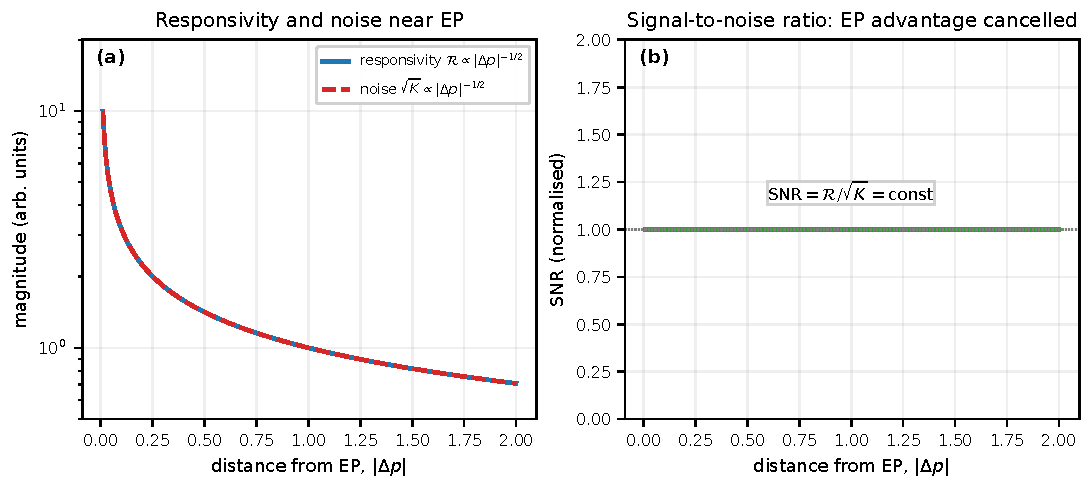
\includegraphics[width=0.95\linewidth]{fig_f18_ep_sensor_tradeoff.pdf}
 \caption{Exceptional-point sensing tradeoff in an idealized
 steady-state, equal-resource model. (a)~Near an EP, the responsivity
 scaling $\mathcal{R}\propto|\Delta p|^{-1/2}$ is accompanied by a
 Petermann-related noise scaling of the same order,
 $\sqrt{K}\propto|\Delta p|^{-1/2}$. The two curves are plotted with
 equal prefactors only to emphasize the shared asymptotic scaling.
 (b)~The corresponding SNR proxy
 $\mathcal{R}/\sqrt{K}$ is therefore approximately constant in this
 model. This illustrates why enhanced frequency splitting alone does
 not guarantee improved measurement precision; a real sensor must be
 judged by its complete noise budget and readout protocol~\cite{wang2020petermann,zhang2018quantum}.}
 \label{fig:ep-sensor-tradeoff}
\end{figure}


Wang et al.\ tested this tradeoff experimentally in a
Brillouin ring laser gyroscope operating near an EP. They measured the
Petermann-factor linewidth broadening and showed that the enhanced
Sagnac splitting was offset by enhanced noise, so that the measured
rotation sensitivity did not improve simply by operating at the
EP~\cite{wang2020petermann}.

\subsection{The noise problem: nonlinear and active systems}
\label{ssec:noise-nonlinear}

Zheng and Chong extended the analysis to nonlinear EP sensors---coupled
cavities operating above the lasing threshold---and showed that
nonlinearity does not rescue the SNR~\cite{zheng2024noise}. Their
analysis revealed three mechanisms by which noise degrades nonlinear
EP sensing:

\begin{enumerate}
 \item \textbf{Noise-induced EP shifting:} fluctuations in the
 intracavity intensity shift the saturated gain, moving the effective
 operating point away from the EP. The system never actually reaches
 the singular $\epsilon^{1/n}$ responsivity.
 \item \textbf{Order reduction:} the nonlinear steady state reduces
 the effective EP order, weakening the fractional-power enhancement.
 An EP$_2$ in the linear system may behave as an effective EP$_1$
 (no enhancement) in the saturated regime.
 \item \textbf{BdG fluctuation EPs:} the Bogoliubov--de~Gennes
 Hamiltonian governing small fluctuations around the nonlinear steady
 state has its own EP structure, which can produce noise divergences
 stronger than the Petermann estimate from the linear system.
\end{enumerate}

The conclusion is sobering: in the analyzed steady-state protocols,
neither linear nor nonlinear EP sensors achieve a fundamental SNR
advantage over DP sensors under the same resource constraints (same
cavity $\Qfac$, same input power, same integration time).

\subsection{When can EP sensing help?}
\label{ssec:ep-when}

Despite the noise-cancellation results, EP sensing may still offer
practical advantages in specific protocols:
\begin{enumerate}
 \item \textbf{Transient measurements:} reading a short-time ring-down
 can make the enhanced dynamical response easier to observe in a fixed
 bandwidth. The relevant figure of merit is the full transient estimator
 variance, not only the steady-state linewidth.
 \item \textbf{Interferometric readout:} heterodyne or self-heterodyne
 schemes that measure the beat frequency between the two split
 modes may reject technical common-mode noise, even though they do not
 remove the fundamental quantum-noise accounting.
 \item \textbf{Active feedback:} real-time feedback can stabilize
 technical drift of the operating point near the EP. It improves
 practical stability but adds its own measurement noise and control
 bandwidth limits.
 \item \textbf{Exceptional surfaces:} in parameter spaces where EPs
 form codimension-one surfaces rather than isolated points,
 the system can be operated on the exceptional surface without
 fine-tuning, potentially reducing the sensitivity to drift.
\end{enumerate}
The general lesson is that the \emph{responsivity} of an EP sensor is
genuinely enhanced, but converting that responsivity into enhanced
\emph{precision} requires a measurement protocol whose complete noise
budget is better than the reference sensor. The distinction between responsivity and
precision is a recurrent theme in non-Hermitian device physics and
should be kept in mind whenever an ``enhanced sensitivity'' claim is
evaluated.


%% ================================================================
\section{BIC-based lasers and cavities}
\label{sec:bic-devices}

\subsection{From radiation suppression to lasing threshold}
\label{ssec:bic-laser-device}

Bound states in the continuum (Chapter~\ref{ch:bic-topology}) provide a
fundamentally different route to high-$\Qfac$ lasing. A photonic
crystal slab laser operating near a BIC exploits the topological
suppression of radiation loss to achieve single-mode lasing with high
power and narrow linewidth, without requiring a physical mirror or
cavity boundary.

The lasing condition connects the BIC physics to the Maxwell-level
framework of this book. The radiation quality factor near a BIC scales
as (Section~\ref{ssec:finite-size})
\begin{equation}
 \Qfac_{\mathrm{rad}}(k) \propto \frac{1}{|c(k)|^2},
 \label{eq:bic-q-rad}
\end{equation}
where $c(k)$ is the radiation amplitude introduced in
Section~\ref{ssec:radiation-amplitude}. At a BIC, $c(k_{\mathrm{BIC}}) = 0$
and $\Qfac_{\mathrm{rad}} \to \infty$. Adding gain to the slab
reduces the total quality factor to
\begin{equation}
 \frac{1}{\Qfac_{\mathrm{tot}}} = \frac{1}{\Qfac_{\mathrm{rad}}}
 + \frac{1}{\Qfac_{\mathrm{abs}}} - \frac{1}{\Qfac_{\mathrm{gain}}},
 \label{eq:bic-total-q}
\end{equation}
where $\Qfac_{\mathrm{abs}}$ accounts for material absorption and
$\Qfac_{\mathrm{gain}}$ accounts for optical gain. The lasing threshold
is reached when $\Qfac_{\mathrm{tot}} \to \infty$, i.e.,
\begin{equation}
 \frac{1}{\Qfac_{\mathrm{gain}}} = \frac{1}{\Qfac_{\mathrm{rad}}}
 + \frac{1}{\Qfac_{\mathrm{abs}}}.
 \label{eq:bic-threshold}
\end{equation}
Near the BIC, $\Qfac_{\mathrm{rad}}$ is very large, so the threshold is
determined primarily by material absorption: the BIC suppresses the
radiation channel, leaving only the material loss as the dominant
threshold-setting mechanism. In finite active devices the threshold is
also limited by finite aperture, pump overlap, nonradiative recombination,
and thermal rollover, but radiation suppression is the central reason for
the low thresholds observed in BIC lasers.

The finite-size limitation is set by the momentum spread
$\Delta k \sim 1/N$ of a cavity with $N$ periods. For an isolated
charge-one BIC, $\Qfac_{\mathrm{finite}} \propto N^2$, which can be
modest for small cavities.

\subsection{Super-BIC lasers}
\label{ssec:super-bic-device}

The topological charge-merging strategy of Section~\ref{sec:bic-merging}
can improve the finite-size scaling. When symmetry and
charge conservation force the lower-order radiation amplitudes to cancel
at the merged point, the radiation amplitude vanishes to higher order:
\begin{equation}
 c(k) \propto k^{|q|} \quad \Longrightarrow \quad
 \Qfac_{\mathrm{finite}} \propto N^{2|q|}.
 \label{eq:super-bic-scaling}
\end{equation}
For the super-BIC design discussed in Chapter~\ref{ch:bic-topology}, the
leading radiation rate scales as $k^6$, so the finite-size $\Qfac$ can
scale as $N^6$, compared with the $N^2$ scaling of an
isolated BIC. This scaling is not guaranteed by charge addition alone;
it also relies on the symmetry of the merged configuration.

Hwang et al.\ demonstrated a super-BIC laser in an InGaAsP photonic
crystal slab with a square lattice of air holes~\cite{hwang2021ultralow}.
By tuning the lattice constant to the merging point
($a \approx \SI{576.3}{nm}$), they achieved:
\begin{itemize}
 \item Radiation loss scaling of $k^6$ instead of $k^2$.
 \item Measured threshold of $\sim\SI{1.47}{kW/cm^2}$---roughly
 $50$ to $10^7$ times lower than previous BIC nanolasers.
 \item Quality factor up to $\sim 7300$ in a cavity of only
 $15 \times 15$ periods.
 \item A strongly confined far-field image consistent with the $k^6$
 angular suppression.
\end{itemize}
The super-BIC concept demonstrates that topological charge engineering
can convert a fundamental limitation (the finite-size $\Qfac$ penalty)
into a practical design advantage.

\subsection{BZF-BIC cavities}
\label{ssec:bzf-device}

Brillouin-zone-folding BICs (Section~\ref{sec:bzf-bic}) offer a
complementary approach: instead of steepening the $\Qfac$ scaling at a
single $k$-point, they sustain high $\Qfac$ over a broad momentum
range. Wang et al.\ showed that BZF-BICs retain $\Qfac$ at least ten
times higher than conventional BICs under the same structural
disorder~\cite{wang2023brillouin}, making them attractive for large-area
lasing and sensing applications where momentum-space averaging is
important.

\subsection{Quasi-BIC applications beyond lasing}
\label{ssec:quasi-bic-apps}

Away from the exact BIC condition, the system supports a quasi-BIC
resonance with finite but very large $\Qfac$. The quasi-BIC produces
a sharp Fano line shape in the scattering spectrum
(Section~\ref{ssec:quasi-bic-resonances}), which is useful for applications beyond
lasing:
\begin{itemize}
 \item \textbf{Refractive-index sensing:} the figure of merit
 $\mathrm{FOM}=S/\delta\lambda
 = \Delta\lambda/(\Delta n\,\delta\lambda)$,
 where $S=\Delta\lambda/\Delta n$ is the sensitivity,
 $\delta\lambda$ is the linewidth, and $\Delta n$ is the index change, benefits
 directly from the high $\Qfac$ of the quasi-BIC. Reported FOMs
 for quasi-BIC metasurfaces exceed $10^3$ in the near-infrared.
 \item \textbf{Nonlinear enhancement:} resonant field buildup can
 strongly enhance nonlinear conversion, with the precise power of
 $\Qfac$ depending on whether the pump, signal, and generated frequency
 are all resonant and critically coupled. This makes quasi-BIC
 resonances attractive platforms for nonlinear nanophotonics, but the
 scaling is device- and process-dependent.
 \item \textbf{Spectral filtering:} the asymmetric Fano profile of a
 quasi-BIC can be engineered to produce narrow-band filters with
 tunable center wavelength and bandwidth by adjusting the structural
 perturbation that breaks the BIC condition.
\end{itemize}


%% ================================================================
\section{Coherent perfect absorbers and switches}
\label{sec:cpa-devices}

\subsection{CPA as a scattering zero}
\label{ssec:cpa-switch}

A coherent perfect absorber (Section~\ref{ssec:zeros}) operates at a zero
of the scattering matrix: with the correct phase and amplitude
relationship between two input beams, all light is absorbed. From the
pole-zero framework of Chapter~\ref{ch:poles-zeros}, the CPA condition
corresponds to a real-frequency zero of $\det S(\omega)$.

The CPA device functions as an all-optical switch: modulating the
relative phase $\phi$ between the two input beams sweeps the system
between perfect absorption ($\phi = \phi_0$) and near-total
transmission ($\phi = \phi_0 + \pi$). The switching contrast is
\begin{equation}
 \mathcal{C} = \frac{T_{\max}}{T_{\min}}
 = \frac{(1 + |r|)^2}{(1 - |r|)^2},
 \label{eq:cpa-contrast}
\end{equation}
where $|r|$ is the single-channel reflection coefficient at the CPA
frequency. For $|r| \to 1$ (high-finesse cavity), the contrast diverges,
but in practice it is limited by absorption losses and fabrication
imperfections.

The switching speed is set by the cavity lifetime
$\tau = \Qfac/\omega_0$; for a $\Qfac \sim 10^3$ resonator at
$\lambda = 1550\;\mathrm{nm}$, $\tau \approx 0.8\;\mathrm{ps}$---faster
than electronic switches by orders of magnitude.

\begin{figure}[t]
 \centering
 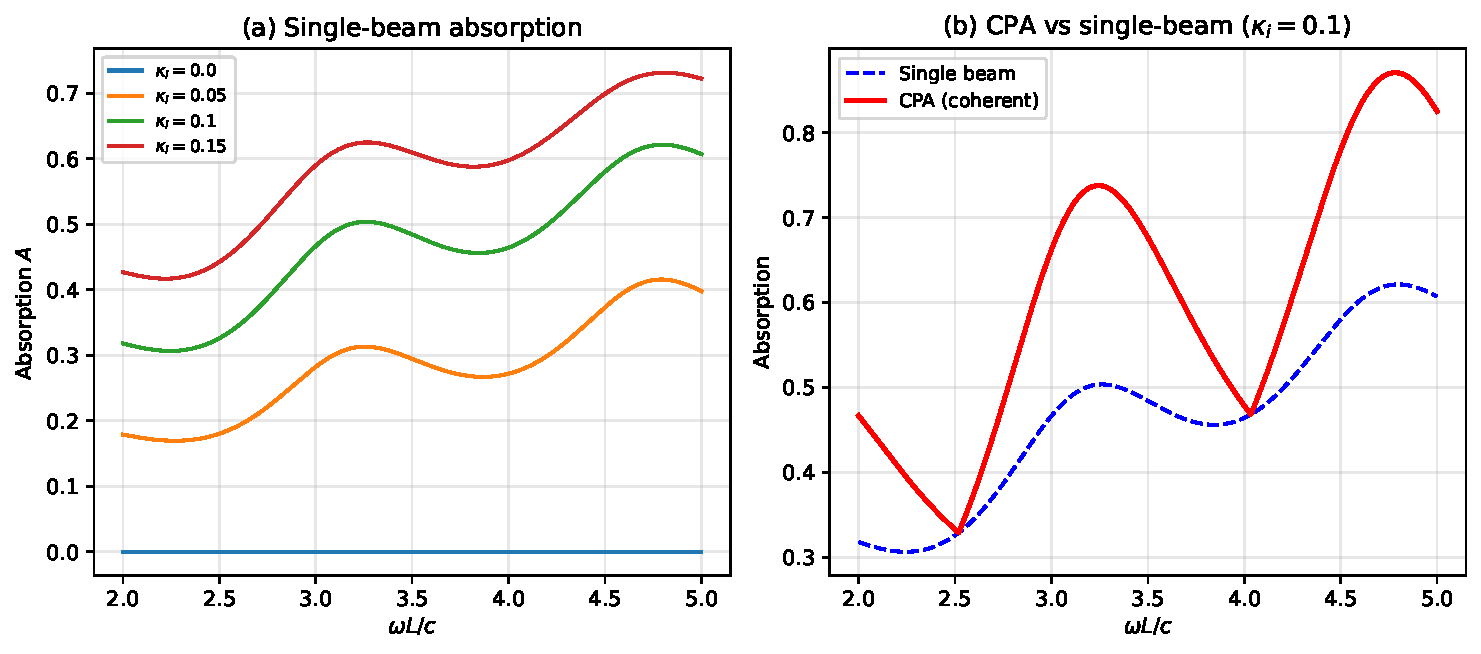
\includegraphics[width=0.85\linewidth]{figures/fig_f18_cpa_switching.pdf}
 \caption{Coherent perfect absorption in a lossy Fabry--P\'erot cavity
 ($n = 2$).
 (a)~Single-beam absorption for different extinction coefficients
 $\kappa_i$: increasing material loss raises the peak absorption but
 broadens the resonance.
 (b)~Comparison of single-beam (dashed) and coherent two-beam (solid)
 absorption for $\kappa_i = 0.1$. Under coherent illumination the
 absorption reaches near-unity at the CPA frequency, demonstrating the
 interferometric enhancement that is the hallmark of CPA---the
 time-reversed counterpart of lasing
 (Section~\ref{sec:time-reversal}).}
 \label{fig:cpa-switching}
\end{figure}

\subsection{CPA-laser devices}
\label{ssec:cpa-laser-device}

At the CPA-laser point (Chapter~\ref{ch:poles-zeros}), the same device
simultaneously acts as a laser (for one input configuration) and a
perfect absorber (for the conjugate configuration). From the scattering
matrix formalism, this corresponds to
\begin{equation}
 \det S(\omega_{\mathrm{CPA\text{-}laser}}) = 0
 \quad \text{and} \quad
 \det S(\omega_{\mathrm{CPA\text{-}laser}}) \text{ has a pole},
 \label{eq:cpa-laser-condition}
\end{equation}
i.e., a simultaneous pole and zero at the same real frequency. In a
$\PT$-symmetric system, the symmetry constrains poles and zeros to occur
in conjugate pairs (Section~\ref{sec:pt-scattering}), making the
CPA-laser condition possible when a pole and its time-reversed zero meet
on the real axis. The symmetry is a constraint, not by itself a guarantee
that a real-frequency pole-zero coincidence occurs without tuning.

The dual CPA-laser functionality enables phase-controlled routing: by
tuning the input phase, the device can be switched between amplification
and absorption, with the transition controlled by the pole-zero
structure of the scattering matrix.

The practical challenge is maintaining the precise gain--loss balance
required by the CPA-laser condition. Any imbalance shifts the pole
and zero apart, reducing the contrast. The critical distinction,
emphasized in Section~\ref{ssec:cpa-vs-ep}, is that the CPA-laser
condition depends on fine-tuned scattering singularities, not on
topological invariants. Topological protection (from BIC charges or
Chern edge states) does \emph{not} protect the CPA-laser point, because
a topological invariant constrains the \emph{number} of singularities in
a region of parameter space, not their \emph{positions}.

\subsection{Practical CPA limitations}
\label{ssec:cpa-limits}

Several practical constraints limit CPA device performance:
\begin{itemize}
 \item \textbf{Beam alignment:} perfect absorption requires precise
 control of the phase, amplitude, and spatial mode of two input
 beams. Any mismatch reduces the absorption efficiency.
 \item \textbf{Bandwidth:} the CPA condition is satisfied at a single
 frequency; broadband operation requires a resonator design with
 overlapping or broadened zeros.
 \item \textbf{Nonlinear effects:} at high input powers, the CPA
 condition shifts due to Kerr and thermal nonlinearities, limiting
 the useful power range.
\end{itemize}


%% ================================================================
\section{Topological lasers}
\label{sec:topo-lasers}

\subsection{Topological insulator lasers}
\label{ssec:topo-laser}

A topological insulator laser~\cite{bandres2018topological,harari2018topological} combines a photonic topological insulator
(Chapter~\ref{ch:berry-maxwell}) with optical gain. The lasing mode
propagates along the topological edge channel, where elastic
backscattering from fabrication defects is strongly suppressed as long as the
topological gap and the protecting symmetries are maintained. The result
can be a laser with robust single-mode operation and high slope
efficiency, but gain competition, disorder-induced loss, and finite-size
coupling still matter.

Several platforms have demonstrated topological lasing:
\begin{itemize}
 \item \textbf{Microring arrays:} coupled microring resonators with
 alternating link-ring couplers that implement a photonic
 anomalous quantum Hall lattice. Bandres et al.\ (2018)
 demonstrated edge-mode lasing with a slope efficiency comparable
 to conventional ring lasers but with improved
 robustness against intentional defects---removing a ring from the
 edge path did not suppress lasing, whereas removing a bulk-mode
 ring had no effect.
 \item \textbf{Valley-Hall photonic crystals:} triangular-hole
 photonic crystal slabs with broken inversion symmetry, supporting
 valley-polarized edge states. Lasing along the domain wall was
 shown to be robust against sharp $120^\circ$ bends, with
 threshold comparable to the straight-edge case.
 \item \textbf{SSH micropillar chains:} one-dimensional arrays of
 semiconductor micropillars with alternating coupling, where
 topological edge modes lase selectively at the chain boundary.
 The topological gap protects the edge state from hybridizing
 with bulk modes, providing a natural single-mode filter.
\end{itemize}

The key metric for a topological laser is not the absolute threshold or
slope efficiency---these are comparable to conventional lasers---but
rather the \emph{robustness} of the single-mode operation and the
\emph{insensitivity} to disorder.

\subsection{Non-Hermitian topological lasers}
\label{ssec:nh-topo-laser}

Adding non-Hermitian ingredients (gain/loss patterning, $\PT$ symmetry)
to topological structures creates a richer design space. For example,
selectively pumping only the edge region of a topological lattice can
enforce single-mode topological lasing without requiring uniform gain
across the entire structure---reducing the power budget and avoiding
multimode instabilities from bulk gain.

This strategy exploits non-Hermitian gain selectivity rather than the
skin effect by itself: patterning the imaginary part of the on-site
potential to provide gain only near the boundary preferentially amplifies
edge modes and suppresses bulk modes. If the underlying lattice also has
point-gap winding, true skin accumulation can further reshape the modal
profiles, but boundary pumping alone should not be identified with the
NHSE.

An important distinction is between \emph{topological protection of
the lasing mode} and \emph{topological origin of the lasing
threshold}. In most topological lasers~\cite{ota2020active,zhu2026topology,al2024topological}, the topology protects the
spatial profile of the lasing mode (preventing backscattering and
maintaining single-mode character), but the threshold itself is set by
the gain--loss balance, which is not topologically protected.

\subsection{Non-Hermitian skin amplifiers}
\label{ssec:skin-amplifier}

The standard non-Hermitian skin effect localizes an extensive set of
right eigenstates at one boundary
(Chapter~\ref{ch:skin-effect}). In a system with gain, this
localization produces exponential amplification of signals injected at
the opposite boundary, as they propagate toward the skin-effect edge.
Using the Hatano--Nelson model of Section~\ref{sec:hatano-nelson}, the
ideal amplitude factor grows exponentially with system size:
\begin{equation}
 G = \left(\frac{t_R}{t_L}\right)^L,
 \label{eq:skin-gain}
\end{equation}
where $t_R/t_L$ is the hopping asymmetry ratio and $L$ is the number of
unit cells. If $G$ is interpreted as a power gain, the corresponding dB
value is $10\log_{10}G$; if it is a field-amplitude factor, the power
gain scales as $|G|^2$. For $t_R/t_L=2$ and $L=20$, the ideal amplitude
factor is $2^{20}\approx10^6$, corresponding to an enormous small-signal
power gain before saturation and noise are included.

The direction of accumulation is tied to the sign of the point-gap
winding of the PBC spectrum around the reference energy
(Section~\ref{sec:winding}). This provides a route to directional
amplification without necessarily using magneto-optical materials,
although a physical photonic implementation must still realize effective
asymmetric hopping and control added noise.

The practical challenge is implementing the required asymmetric hopping
in a photonic platform. Photonic mesh lattices with fiber loops of
different lengths, time-modulated coupled resonators, and
magnetically biased photonic crystals have been proposed as physical
realizations.


%% ================================================================
\section{Active non-Hermitian metasurfaces}
\label{sec:nh-metasurfaces}

\subsection{Wavefront control with gain and loss}
\label{ssec:nh-wavefront}

Non-Hermitian metasurfaces~\cite{cui2024roadmap,ma2022information} extend the wavefront-control capabilities of
passive metasurfaces by incorporating gain and loss as additional design
degrees of freedom. In a passive metasurface, each meta-atom controls
the phase and amplitude of the transmitted or reflected field through
its geometric and material parameters. In a non-Hermitian metasurface,
each meta-atom additionally carries a complex refractive index with a
controllable imaginary part, enabling independent control of the phase,
amplitude, and gain/loss profile across the surface.

From the scattering-matrix perspective (Chapter~\ref{ch:poles-zeros}),
each meta-atom is characterized by its complex transmission and
reflection coefficients. By engineering the pole-zero structure of each
meta-atom, the metasurface can implement arbitrary complex transfer
functions, achieving functionalities impossible with purely passive
elements---for example, asymmetric reflection profiles where the
reflected wavefront depends on the illumination direction.

\subsection{$\PT$-symmetric metasurfaces}
\label{ssec:pt-metasurface}

A metasurface with a $\PT$-symmetric gain/loss distribution can exhibit
unidirectional properties analogous to those of $\PT$-symmetric Bragg
gratings (Section~\ref{ssec:unidirectional}). At the $\PT$-breaking
point, the metasurface can be invisible from one side while reflecting
from the other, creating a flat-optics analogue of unidirectional
invisibility.

\subsection{CPA metasurfaces}
\label{ssec:cpa-metasurface}

A metasurface designed to operate at the CPA condition provides a
thin-film all-optical modulator. By controlling the relative phase
of two counter-propagating beams incident on the metasurface, the
absorption can be switched from near-zero to near-unity, enabling
modulation at sub-picosecond timescales with a device footprint of
a single wavelength.


%% ================================================================
\section{Physical limits}
\label{sec:physical-limits}

Every non-Hermitian device advantage comes with a physical cost. This
section catalogs the principal limits in a unified framework and
provides quantitative estimates that allow device designs to be compared
on an equal footing.

\subsection{Quantum noise and the Petermann factor}
\label{ssec:quantum-noise}

All non-Hermitian photonic devices are ultimately limited by quantum
noise. The fluctuation-dissipation theorem requires that any system with
loss also has noise; gain media amplify both signal and spontaneous
emission. Near an EP, the enhanced Petermann
factor~\eqref{eq:petermann-linewidth} amplifies the noise, setting a
fundamental floor on the sensitivity of EP-based devices.

The Petermann factor reflects the non-orthogonality of the modes in the
biorthogonal expansion of Chapter~\ref{ch:qnm}. In a system with
$K_{\mathrm{P}} = 100$ (easily achieved within
$|\Delta p|/\kappa \sim 0.1$ of a second-order EP), the spontaneous
emission rate into the lasing mode is enhanced by a factor of 100
relative to the Hermitian limit, degrading the laser coherence and the
sensor precision by the same factor.

For an $n$th-order EP, the Petermann factor diverges as
(Section~\ref{ssec:petermann-ep})
\begin{equation}
 K_{\mathrm{P}} \propto \frac{1}{|\Delta p|^{2(n-1)}},
 \label{eq:petermann-scaling-device}
\end{equation}
where $\Delta p$ is the distance from the EP in parameter space. The
noise penalty therefore grows faster with EP order than the responsivity
enhancement ($\epsilon^{1/n}$), and the net SNR actually \emph{decreases}
with increasing EP order for fixed resource constraints.

\subsection{Gain saturation and nonlinearity}
\label{ssec:nonlinearity-limits}

The linear non-Hermitian framework of this book is valid below or near
the lasing threshold. Above threshold, gain saturation introduces
nonlinear corrections that stabilize the system (preventing runaway
amplification) but also modify the EP structure and the topological
invariants.

The gain saturation model of Section~\ref{sec:gain-media} gives
\begin{equation}
 g(I) = \frac{g_0}{1 + I/I_{\mathrm{sat}}},
 \label{eq:gain-saturation-device}
\end{equation}
where $g_0$ is the small-signal gain, $I$ is the intracavity intensity,
and $I_{\mathrm{sat}}$ is the saturation intensity. For EP sensors
operating above threshold, the nonlinear steady state shifts the
operating point away from the EP by an amount
\begin{equation}
 \delta g \sim g_0 \frac{I_{\mathrm{ss}}}{I_{\mathrm{sat}}},
 \label{eq:ep-shift-nonlinear}
\end{equation}
where $I_{\mathrm{ss}}$ is the steady-state intracavity intensity. This
shift effectively reduces the EP order and weakens the $\epsilon^{1/n}$
responsivity~\cite{zheng2024noise}.

For topological invariants, gain saturation can change the sign of the
imaginary part of the permittivity, potentially opening or closing
point gaps and modifying the winding numbers. The interplay between
nonlinearity and non-Hermitian topology is an active research frontier
(Chapter~\ref{ch:open-problems}).

\subsection{Fabrication disorder}
\label{ssec:disorder}

Real photonic devices have fabrication imperfections that perturb the
$\PT$ symmetry condition, shift EPs, and break the gain--loss balance.
Different non-Hermitian features have different robustness:
\begin{itemize}
 \item \textbf{Topologically constrained:} BIC far-field charges
 (Section~\ref{sec:bic-charge}), Chern edge states, and
 point-gap/skin-effect orientation are robust to perturbations that
 preserve the relevant gap, symmetry, and radiation-channel structure.
 They change only when the corresponding topological description breaks
 down or a topological transition occurs.
 \item \textbf{Fine-tuned:} the precise EP location, the CPA-laser
 condition, the $\PT$ symmetry balance, and the gain--loss
 threshold all depend on continuous parameters and are shifted
 by any fabrication error.
\end{itemize}
The practical design challenge is to maximize the fraction of the device
functionality that relies on topological protection, while accepting
that fine-tuned parameters will need active stabilization or tolerance
engineering.

A useful figure of merit for disorder robustness is the \emph{topological
gap ratio}---the ratio of the topological gap $\Delta_{\mathrm{top}}$
to the typical disorder-induced level broadening $\Gamma_{\mathrm{dis}}$.
When $\Delta_{\mathrm{top}}/\Gamma_{\mathrm{dis}} \gg 1$, topologically
protected features survive; when $\Delta_{\mathrm{top}}/\Gamma_{\mathrm{dis}}
\lesssim 1$, the topological protection breaks down and device
performance reverts to the non-topological baseline.

\subsection{Thermal and power limits}
\label{ssec:thermal}

Gain media dissipate heat. In semiconductor lasers, the thermal load
from the pump current limits the maximum gain that can be applied before
thermal rollover degrades the performance. $\PT$-symmetric devices,
which require a precise balance between gain and loss, are particularly
sensitive to thermal drifts because the gain medium and the loss medium
have different thermal coefficients.

For BIC-based devices, the ultra-high $\Qfac$ near the BIC reduces the
threshold power, mitigating the thermal problem. The super-BIC laser of
Hwang et al.\ achieved a threshold of $\sim\SI{1.47}{kW/cm^2}$---orders
of magnitude below conventional nanolasers---precisely because the
topological charge merging minimized the radiation
loss~\cite{hwang2021ultralow}.

\subsection{Gain--bandwidth constraints}
\label{ssec:gain-bandwidth}

A fundamental constraint on non-Hermitian devices comes from the
gain--bandwidth product. The Kramers--Kronig relations
(Section~\ref{sec:kramers-kronig}) link the real and imaginary parts
of the permittivity, so gain over a finite bandwidth implies a
corresponding frequency-dependent phase shift. For a Lorentzian gain
medium with peak gain $g_0$ and gain bandwidth $\Delta\omega_g$, the
gain--bandwidth product is
\begin{equation}
 g_0 \cdot \Delta\omega_g = \frac{N_{\mathrm{inv}}\,\sigma_0\,c}{n_g},
 \label{eq:gain-bandwidth}
\end{equation}
where $N_{\mathrm{inv}}$ is the population inversion density,
$\sigma_0$ is the stimulated emission cross-section, and $n_g$ is the
group index. This places an upper bound on the gain that can be
achieved over a given bandwidth, limiting the number of modes that can
be simultaneously pushed above threshold in a $\PT$-symmetric laser
and constraining the operational bandwidth of EP sensors.

\subsection{Summary: device concepts and their physical limits}
\label{ssec:device-summary}

\begin{figure}[t]
 \centering
 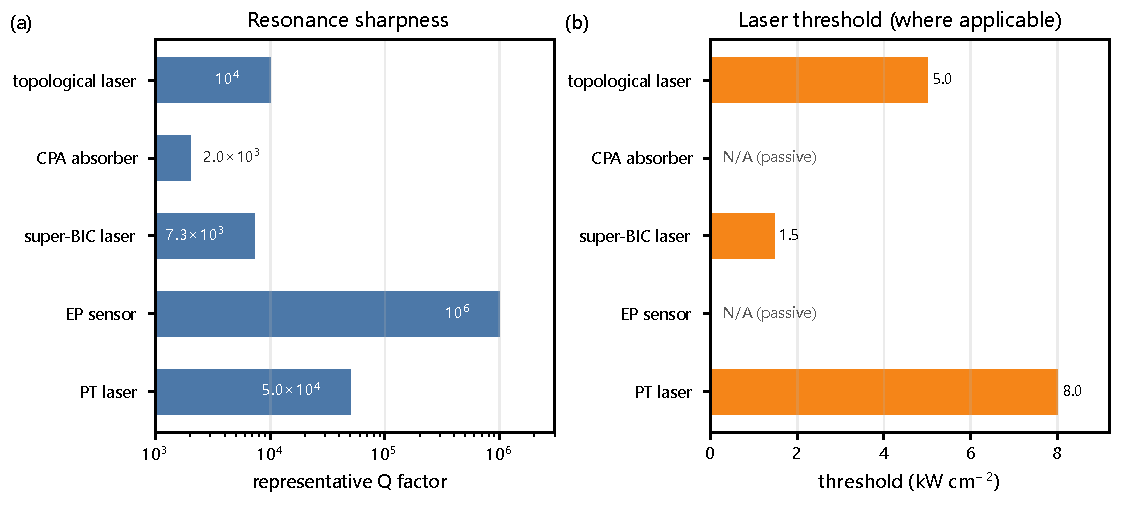
\includegraphics[width=0.95\linewidth]{fig_f18_device_comparison.pdf}
 \caption{Quantitative comparison of five non-Hermitian photonic device
 classes discussed in this chapter.
 (a)~Representative quality factor $\Qfac$ on a logarithmic scale.
 The EP sensor achieves the highest $\Qfac \sim 10^6$ through
 whispering-gallery modes, while the CPA absorber operates at a
 modest $\Qfac \sim 2 \times 10^3$ because critical coupling demands
 matched radiative and absorptive rates.
 (b)~Lasing threshold in kW\,cm$^{-2}$ for laser-type devices; the
 EP sensor and CPA absorber are passive and marked N/A. The
 super-BIC laser has the lowest threshold
 ($1.47\;\mathrm{kW\,cm}^{-2}$) thanks to the $k^6$
 radiation-loss suppression of merged BICs. Data are representative
 values from the literature discussed in the text.}
 \label{fig:device-comparison}
\end{figure}

Table~\ref{tab:device-limits} summarizes the principal non-Hermitian
device concepts, their key operating mechanisms, the source of
their non-Hermitian advantage, and the physical limit that constrains
their performance.

\begin{table}[t]
\centering
\small
\caption{Non-Hermitian photonic device concepts and their physical limits.}
\label{tab:device-limits}
\begin{tabular}{@{}p{3.0cm}p{3.2cm}p{3.2cm}p{3.8cm}@{}}
\toprule
\textbf{Device} & \textbf{Mechanism} & \textbf{NH advantage} & \textbf{Primary limit} \\
\midrule
$\PT$ laser & EP mode selection & Single-mode purity & Petermann noise, thermal drift \\
EP sensor & $\epsilon^{1/n}$ splitting & Enhanced responsivity & Petermann noise cancels SNR gain \\
BIC laser & Topological $\Qfac$ & Ultralow threshold & Finite-size $\Qfac$, disorder \\
Super-BIC laser & Charge merging & Steeper finite-size $\Qfac$ scaling & Lattice-constant tolerance \\
CPA switch & Scattering zero & All-optical modulation & Beam alignment, bandwidth \\
CPA-laser & Pole-zero coincidence & Dual amplification/absorption & Fine-tuned gain--loss balance \\
Topological laser & Edge-state lasing & Disorder robustness & Threshold not topologically protected \\
Skin amplifier & NHSE localization & Directional small-signal gain & Asymmetric hopping, saturation, noise \\
\bottomrule
\end{tabular}
\end{table}

\begin{takeaway}[Promise and limits of non-Hermitian devices]
Non-Hermitian photonic devices exploit exceptional points, $\PT$
symmetry, CPA-laser duality, BIC topology, and the skin effect to
achieve functionalities impossible in Hermitian systems: single-mode
lasing, enhanced sensing responsivity, all-optical switching, and
directional amplification. But every advantage comes with a physical
cost---the Petermann noise penalty, gain saturation, fabrication
sensitivity, or thermal load---that must be assessed quantitatively
against the specific application. The most robust devices are those
that anchor their functionality in topological invariants rather than
fine-tuned parameters, and the most honest assessments compare not just
the enhanced response but the enhanced response \emph{together with}
the enhanced noise.
\end{takeaway}

\chapter{Open Problems and Outlook}
\label{ch:open-problems}

\begin{chapterlead}
Non-Hermitian photonics is a young and rapidly developing field. Many
fundamental questions remain open, and new experimental platforms
continue to reveal unexpected phenomena. This final chapter surveys the
frontier as a set of tensions that drive the field forward. Each section identifies a
concrete gap between the theoretical framework of this book and the
physics that lies beyond it, explains why the gap matters, and points
toward the ideas that may close it.
\end{chapterlead}

\begin{figure}[t]
 \centering
 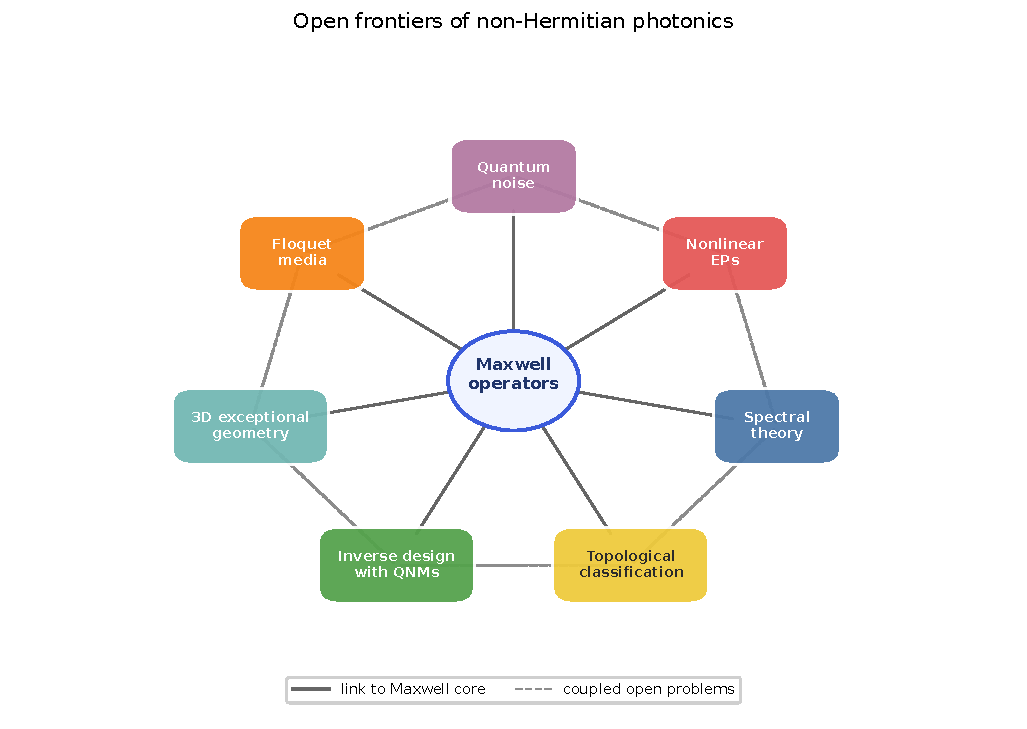
\includegraphics[width=0.82\linewidth]{fig_f19_frontier_landscape.pdf}
 \caption{Seven coupled frontiers of Maxwell-first non-Hermitian
 photonics. Solid lines connect each frontier to the central Maxwell
 operator framework developed in this book; dashed lines indicate
 cross-frontier couplings where progress on one problem constrains or
 enables another. The frontiers are: nonlinear exceptional points
 (EPs), quantum noise limits, Floquet-driven media, three-dimensional
 exceptional geometry, inverse design via quasinormal modes (QNMs),
 rigorous spectral theory, and topological classification beyond
 two dimensions. Each is discussed in a section of this chapter.}
 \label{fig:frontier-landscape}
\end{figure}

%% ================================================================
\section{Nonlinear non-Hermitian photonics}
\label{sec:nonlinear-nh}

\subsection{Why linearity is not enough}
\label{ssec:nonlinear-why}

The entire theoretical framework of this book assumes linear media: the
permittivity $\epsr$ is independent of the field amplitude, and the
Maxwell operator is a fixed linear map. This assumption breaks down in
two physically important regimes:
\begin{enumerate}
 \item \textbf{Above the lasing threshold.} Once gain exceeds loss in
 a cavity mode, the field amplitude grows exponentially until gain
 saturation---a nonlinear effect---clamps it. The steady-state
 amplitude is set by the balance between saturated gain and loss,
 not by the linear eigenproblem.
 \item \textbf{Strongly driven systems.} High-intensity light in a
 Kerr medium modifies the refractive index as
 $n_{\mathrm{eff}} = n_0 + n_2\,|E|^2$, creating an
 intensity-dependent effective Hamiltonian. In a non-Hermitian system,
 the Kerr shift can move the system toward or away from an exceptional
 point, coupling the EP physics to the field dynamics.
\end{enumerate}

\subsection{Gain saturation and the fate of exceptional points}
\label{ssec:gain-saturation-open}

Gain saturation introduces a nonlinear self-consistency problem: the
effective Hamiltonian depends on the field amplitudes, which in turn
depend on the Hamiltonian. Near an EP, the consequences are subtle.
Zheng and Chong showed that in a coupled-cavity laser system, noise
fluctuations shift the operating point away from the EP, effectively
reducing the EP order and preventing the system from exploiting the full
$\epsilon^{1/n}$ responsivity~\cite{zheng2024noise}. Moreover, the
linearized Bogoliubov--de~Gennes (BdG) Hamiltonian governing small fluctuations
around the nonlinear steady state has its \emph{own} EP structure, which
can produce noise divergences \emph{stronger} than the simple Petermann
estimate from the linear system.

This result challenges the premise that operating a sensor near a linear
EP automatically confers a metrological advantage. A full theory of
nonlinear EP sensing must
treat the noise, the nonlinearity, and the EP on an equal footing,
rather than analyzing the linear EP first and adding noise afterward.

\subsection{Nonlinear topology}
\label{ssec:nonlinear-topology}

Can topological invariants survive in a nonlinear system? For Kerr-type
nonlinearity, Xia et al.\ demonstrated experimentally that local
intensity-dependent refractive index changes can tune the global $\PT$
symmetry of a waveguide lattice, restoring or destroying non-Hermitian
topological states~\cite{xia2021nonlinear}. This suggests that
nonlinearity does not simply destroy topology: in suitable driven
systems it can create an intensity-dependent topological phase
diagram~\cite{zhen2023nonlinear,xia2021nonlinear,szameit2020nonlinearity,leykam2016edge,li2022topological,kartashov2024solitons,tang2022vector}.

A systematic theory of nonlinear non-Hermitian topology~\cite{rechtsman2013photonic,kim2020recent,maczewsky2017observation,kitagawa2010topological,rudner2013anomalous,nathan2017anomalous,guglielmon2017photonic,farrell2016edge} is still
missing. The obstacles include:
\begin{itemize}
 \item Topological invariants are defined for linear eigenproblems;
 extending them to nonlinear fixed-point problems requires new
 mathematical tools.
 \item The skin effect, which depends on the spectral winding of the
 \emph{linear} Hamiltonian, may be modified or destroyed by
 nonlinear mode coupling.
 \item Solitons in $\PT$-symmetric systems form continuous families
 rather than the isolated amplitude values found in generic
 dissipative systems~\cite{wimmer2015observation,alexeeva2012optical,mukherjee2021observation,johansson2025floquet,shen2023floquet,chen2025nonlinear};
 the stability and topological classification of these families remain
 open problems.
\end{itemize}

\paragraph{Open problem: nonlinear EP laser dynamics.}
Consider a pair of coupled ring resonators with Kerr nonlinearity,
modelled by
\begin{equation}
 i\frac{\dd}{\dd t}
 \begin{pmatrix} a_1 \\ a_2 \end{pmatrix}
 =
 \begin{pmatrix}
 \omega_0 + g(|a_1|^2) + i\gamma_1 & \kappa \\
 \kappa & \omega_0 + g(|a_2|^2) - i\gamma_2
 \end{pmatrix}
 \begin{pmatrix} a_1 \\ a_2 \end{pmatrix},
 \label{eq:nonlinear-ep-laser}
\end{equation}
where $g(I) = g_0/(1 + I/I_{\mathrm{sat}})$ models gain saturation
and $\gamma_2$ represents linear loss. At low intensity the system
approaches a linear EP when $|\gamma_1 - \gamma_2| = 2|\kappa|$. But
as $|a_1|^2$ grows, the saturated gain shifts $\gamma_1$ downward,
and the instantaneous Hamiltonian moves \emph{away} from the EP.
The resulting limit cycle oscillates between near-EP and far-from-EP
regimes, producing a characteristic ``EP breathing'' in the output
intensity. Whether this breathing mode has any robust dynamical
signature tied to the nearby degeneracy---or whether it is a generic
feature of nonlinear saddle--node bifurcations near non-Hermitian
degeneracies---is an open question that requires tools from both
dynamical systems theory and non-Hermitian spectral theory.

\paragraph{Gain saturation and the Bogoliubov--de~Gennes connection.}
The fluctuation dynamics around a nonlinear steady state are governed by
a Bogoliubov--de~Gennes (BdG) Hamiltonian that couples the signal and
idler quadratures. Zheng and Chong showed that the BdG Hamiltonian can
have its own EP structure that is \emph{different} from the EP of the
underlying nonlinear Hamiltonian~\cite{zheng2024noise}. The BdG EP can
produce noise divergences that scale with a Petermann factor computed
from the BdG eigenvectors, not from the original linearized system
alone. This ``BdG Petermann effect'' is a nonlinear extension of the
linear excess-noise mechanism. Its experimental signature---anomalous
linewidth broadening controlled by the fluctuation operator rather than
only by the instantaneous mean-field Hamiltonian---has not yet been
isolated.


%% ================================================================
\section{Quantum non-Hermitian photonics}
\label{sec:quantum-nh}

\subsection{From effective Hamiltonians to open quantum systems}
\label{ssec:quantum-effective}

The effective non-Hermitian Hamiltonian $H_{\mathrm{eff}}$ used
throughout this book is derived from the full Lindblad master equation
by conditioning on zero quantum jumps. This post-selected description
captures the \emph{conditional} dynamics of the photonic system but
discards the quantum jumps (spontaneous emission events, photon
absorption by the environment) that are essential for a complete picture
of the noise and the measurement statistics.

The quantum noise theory of EP sensors~\cite{zhang2018quantum} shows
that the discarded quantum jumps reintroduce noise channels that can
cancel the apparent EP responsivity enhancement in standard measurement
settings. A consistent quantum theory of non-Hermitian photonics must
therefore start from the full open quantum system---either the Lindblad
equation or the quantum Langevin equations with input--output
formalism---and derive the non-Hermitian effective Hamiltonian as a
limit rather than a postulate.

\subsection{Few-photon non-Hermitian physics}
\label{ssec:few-photon}

Most non-Hermitian photonic experiments operate in the classical regime
(many photons per mode). In the few-photon regime, the effective
Hamiltonian description can break down because the probability of
quantum jumps during the observation time becomes significant. The
interplay of non-Hermiticity, quantum fluctuations, and
photon-number-resolved measurement creates a rich and largely unexplored
landscape.

Specific open questions include:
\begin{enumerate}
 \item Can the non-Hermitian skin effect be observed in a quantum
 photonic simulator with single-photon resolution?
 \item Under what measurement protocol, if any, does the EP
 responsivity enhancement translate into improved precision at the
 single-photon level?
 \item Can quantum error correction or reservoir engineering be used to
 control jump-induced decoherence in non-Hermitian topological
 states~\cite{gao2024quantum,al2024topological,acn2018quantum}?
\end{enumerate}

\subsection{Entanglement and biorthogonality}
\label{ssec:entanglement}

The biorthogonal basis (Appendix~\ref{app:nonnormal}) is a mathematical
tool for expanding observables in a non-Hermitian system. Whether it has
a direct quantum information interpretation---for example, whether the
biorthogonal entanglement entropy captures physically relevant
correlations in an open photonic system---is an open and active question.


%% ================================================================
\section{Time-varying and Floquet non-Hermitian systems}
\label{sec:floquet-nh}

\subsection{Floquet engineering of non-Hermiticity}
\label{ssec:floquet-engineering}

Time-periodic (Floquet) modulation of the refractive index creates
effective non-Hermitian Hamiltonians with periodically driven gain, loss,
and coupling. The Floquet formalism maps the time-dependent problem
onto a static problem in an extended Hilbert space (the Floquet--Bloch
space), where the effective Hamiltonian can exhibit EPs, $\PT$ symmetry,
and topological phases that do not exist in any static system.

\begin{figure}[t]
 \centering
 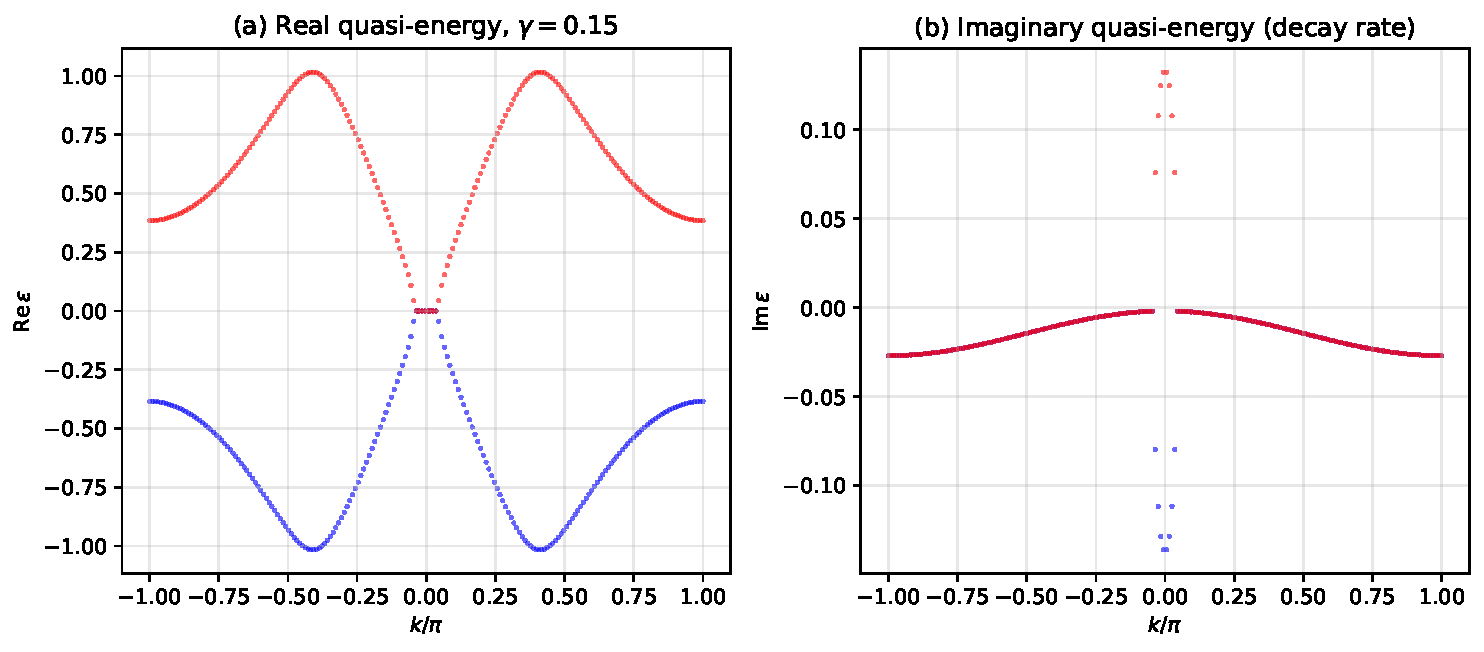
\includegraphics[width=0.85\linewidth]{figures/fig_f19_floquet_bands.pdf}
 \caption{Floquet quasi-energy bands for a periodically driven
 non-Hermitian two-band model ($\gamma = 0.15$, $V = 0.8$,
 $\Omega = 2.5$). (a)~Real part of the quasi-energy $\varepsilon(k)$,
 showing the band structure folded into the Floquet--Brillouin zone.
 (b)~Imaginary part of $\varepsilon(k)$, representing the decay rate.
 The asymmetry between the two bands reflects the non-Hermiticity.}
 \label{fig:floquet-bands}
\end{figure}

\subsection{Floquet exceptional points}
\label{ssec:floquet-ep}

A Floquet EP occurs when two Floquet quasi-energies coalesce---not
necessarily because the instantaneous Hamiltonian has an EP at any fixed
time, but because the time-ordered evolution operator over one period
has a Jordan-block structure. Floquet EPs can be created and controlled
by the modulation amplitude and frequency, providing a temporal knob for
EP physics in addition to spatial design.

\paragraph{Example: periodically modulated coupled cavities.}
Consider two coupled cavities with time-periodic detuning:
$\delta(t) = \delta_0 \cos(\Omega t)$, where $\Omega$ is the
modulation frequency. In the Floquet--Bloch representation, the
effective Hamiltonian becomes an infinite-dimensional matrix coupling
all Floquet harmonics $n\Omega$. A Floquet EP appears when the
modulation amplitude $\delta_0$ reaches a critical value at which two
Floquet quasi-energy bands touch and coalesce. Unlike a static EP, the
degeneracy is defined modulo the drive frequency and can involve
different Floquet replicas; it can therefore be tuned by varying
$\Omega$ or the modulation strength without changing the spatial
geometry. Its stability, however, still depends on the usual
codimension and symmetry constraints of the driven non-Hermitian
operator.

The physical signature is a characteristic beating pattern in the
transient response: near the Floquet EP, the temporal evolution contains
a term proportional to $t\,e^{-i\varepsilon t}$ (the Jordan-block
contribution), producing a linear-in-$t$ envelope modulating the
oscillatory response. This temporal signature is the Floquet analogue
of the spatial mode coalescence at a static EP and can be measured in
the time-domain transmission of a pulsed probe.
\begin{figure}[t]
 \centering
 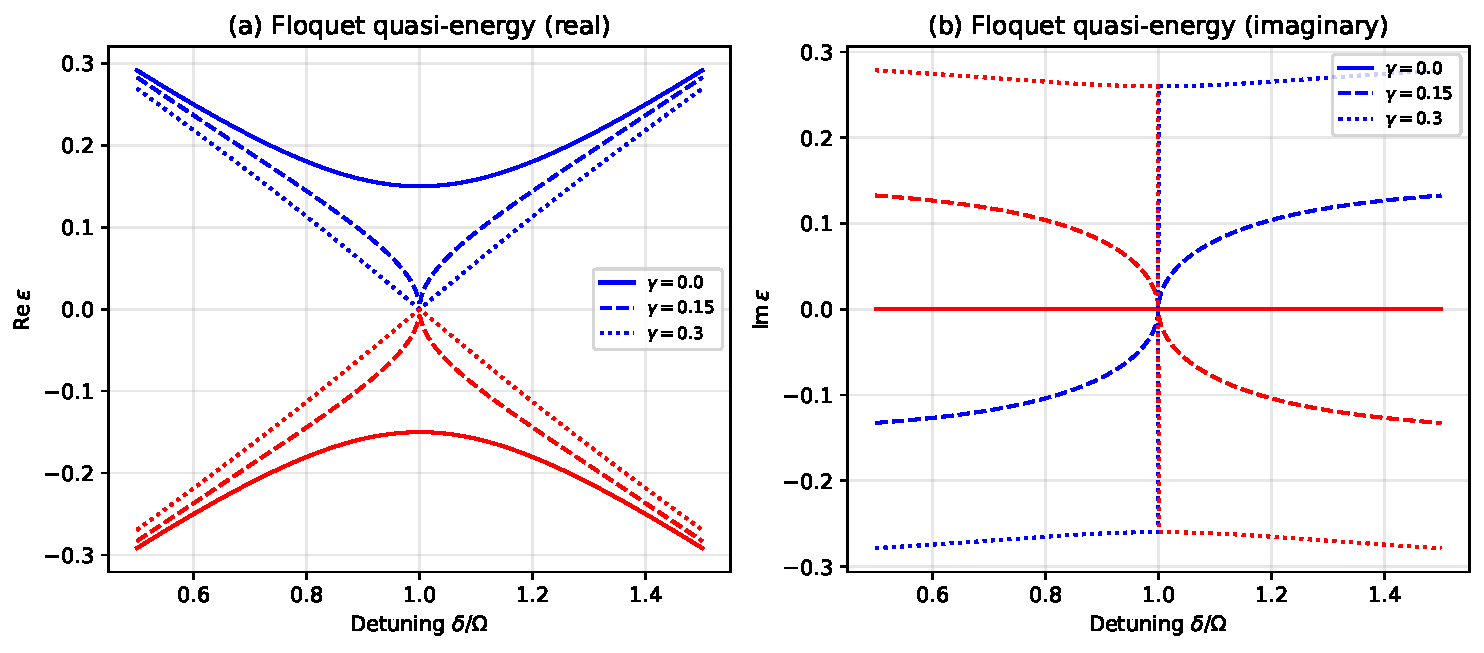
\includegraphics[width=0.85\linewidth]{figures/fig_f19_floquet_ep.pdf}
 \caption{Floquet exceptional point in a periodically driven two-mode
 model. The rotating-wave Floquet Hamiltonian develops quasi-energy
 coalescences controlled by detuning and modulation amplitude.
 (a)~Real quasi-energies show avoided crossings and coalescence as the
 non-Hermitian parameter increases. (b)~Imaginary quasi-energies reveal
 the gain--loss splitting associated with the Floquet EP. The point of
 the figure is not a new device proposal but the mechanism: a time-periodic
 Maxwell system can acquire non-Hermitian degeneracies in Floquet space
 even when no static instantaneous Hamiltonian sits at an EP.}
 \label{fig:floquet-ep}
\end{figure}


\subsection{Open problems}
\label{ssec:floquet-open}

The interplay of temporal and spatial periodicity in non-Hermitian
systems creates several open problems:
\begin{itemize}
 \item A general bulk-boundary correspondence for Floquet
 non-Hermitian systems is not yet established.
 \item The non-Hermitian skin effect in Floquet systems can depend on
 both the driving frequency and the spatial boundary conditions,
 leading to a richer phase diagram than the static case.
 \item Experimental realization of Floquet non-Hermitian photonics
 requires modulation at optical frequencies, which is technically
 demanding but may be achievable with electro-optic modulators or
 optomechanical coupling.
\end{itemize}


%% ================================================================
\section{Non-Hermitian photonics in three dimensions}
\label{sec:3d-nh}

\subsection{Exceptional lines and surfaces}
\label{ssec:3d-topology}

Three-dimensional non-Hermitian photonic crystals support topological
objects that have no lower-dimensional counterpart:
\begin{itemize}
 \item \textbf{Exceptional lines:} one-dimensional curves in the 3D
 Brillouin zone where two bands coalesce. The topology of an
 exceptional line is characterized by a topological charge
 (a $\pi$ Berry phase encircling the line) and a linking number with
 other exceptional lines.
 \item \textbf{Exceptional surfaces:} two-dimensional manifolds of
 degeneracy, which can occur when additional constraints, symmetries,
 or material parameters reduce the effective codimension.
 \item \textbf{Non-Abelian charges:} when three or more bands are
 involved, the braid group replaces the simple winding number, and
 the topological classification becomes non-Abelian.
 \item \textbf{Three-dimensional skin effect:} an extensive set of
 eigenstates can localize on boundaries of a 3D sample, with the
 localization pattern depending on spectral winding and sample geometry.
\end{itemize}

\paragraph{Exceptional lines from Maxwell symmetries.}
In a generic two-band non-Hermitian problem, the EP condition imposes
two real constraints, so in a three-dimensional control space the EP set
is generically a curve. Photonic crystals can realize such control
spaces through Bloch wave vector, material parameters, or symmetry
constraints. The Maxwell vector nature adds polarization structure:
near an exceptional line the coalescing modes may carry a half-integer
vorticity or Berry phase, but the precise relation to polarization
vortices depends on the radiation channels and symmetries of the
particular structure.

\paragraph{Knotted exceptional lines.}
Exceptional lines in 3D can form knots and links. Two exceptional
lines can have a nontrivial linking number, meaning they cannot be
separated by any continuous deformation that preserves the band gap.
This linking is a topological invariant that has no 2D or 1D analogue
and represents a genuinely new form of non-Hermitian topology. Whether
knotted exceptional lines can be realised in a photonic crystal with
practical material parameters is an open fabrication challenge.

\paragraph{3D non-Hermitian skin effect and geometry dependence.}
In three dimensions, the skin effect can become geometry-dependent: the
localization boundary is determined by the interplay of spectral winding
in different spatial directions and the sample shape. In simple
separable models a rectangular sample may exhibit corner accumulation,
whereas other boundary geometries can redistribute the same non-Bloch
decay toward edges or surfaces. The geometry dependence means that the
finite-sample OBC spectrum is not determined by the conventional Bloch
band structure alone.

\subsection{Fabrication and characterization challenges}
\label{ssec:3d-challenges}

Experimental realization of 3D non-Hermitian photonic structures requires
fabrication of three-dimensional lattices with controlled, spatially
varying gain and loss---a significantly harder problem than the 1D or 2D
case. Two-photon lithography, self-assembly, and holographic patterning
are candidate technologies, but none has yet produced a 3D non-Hermitian
photonic crystal with sufficient quality for topological measurements.

Characterization is equally challenging: the 3D bulk--boundary
correspondence predicts surface, hinge, and corner modes that require
spatially resolved measurements in all three dimensions. Near-field
scanning or tomographic reconstruction may be needed.


%% ================================================================
\section{Rigorous spectral theory of open Maxwell operators}
\label{sec:spectral-theory}

\subsection{Completeness of QNM expansions}
\label{ssec:qnm-completeness-open}

The quasinormal-mode expansion (Chapter~\ref{ch:qnm}) is widely used but
not rigorously justified in full generality. The QNMs of an open
resonator form a countable set, but their completeness---in the sense
that any compactly supported source field can be expanded in QNMs---has
been proven only for specific geometries (1D slabs, spheres). For
general 3D resonators with complex shapes and dispersive materials, the
completeness question remains open.

The difficulty is mathematical: QNM fields diverge outside the
resonator (they satisfy outgoing boundary conditions at infinity), so
the expansion converges only in a distributional or regularized sense
(e.g., inside the PML region). A rigorous theory must specify the
function space in which completeness holds and the rate of convergence
of the modal sum.

\paragraph{What a completeness proof would need.}
A satisfactory proof of QNM completeness for a general 3D open Maxwell
system would need to:
\begin{enumerate}
 \item Specify the function space $\mathcal{H}$ of source/field
 distributions (e.g., $L^2$ functions with compact support inside
 the resonator volume).
 \item Prove that the set of QNM fields
 $\{\EE_m(\rr)\}_{m=1}^{\infty}$, regularized by a PML or
 complex-coordinate transformation, is dense in $\mathcal{H}$.
 \item Provide error bounds for the truncated expansion: given $N$
 modes, how large is the remainder in terms of the quality
 factors $Q_m$ and the spectral density near the target
 frequency?
 \item Handle the branch-cut contributions from the continuous
 spectrum (radiation modes), either by including them explicitly
 or by proving that the PML discretizes them into a sequence
 of discrete poles that converges to the branch cut.
\end{enumerate}
A partial result in this direction was obtained for 1D scattering
problems using Mittag-Leffler-type meromorphic expansions of the Green
function. Such results rely on the analytic structure and growth bounds
of the particular scattering problem; extending them to 3D Maxwell
systems with dispersive media requires controlling the Green tensor at
large complex frequency and accounting for branch cuts---nontrivial
analytic estimates.

\subsection{Continuous spectrum and branch cuts}
\label{ssec:continuous-spectrum}

In addition to the discrete QNM poles, the Green tensor of an open
Maxwell system has branch-cut contributions from the continuous spectrum
(radiation modes). These contributions are responsible for the ``PML
modes'' of Chapter~\ref{ch:numerics} and are essential for completeness.
A full modal expansion must include both the discrete poles and the
branch-cut integral, with quantitative estimates for the error of
truncating the branch-cut contribution.

\subsection{Spectral singularities}
\label{ssec:spectral-singularities}

A spectral singularity is a point on the real frequency axis where the
resolvent of the Maxwell operator diverges without an associated
normalizable eigenfunction---it is neither a bound state nor a
scattering resonance, but a divergence of the scattering amplitude.
Spectral singularities have been linked to lasing and CPA in
$\PT$-symmetric systems, but their mathematical theory (existence,
genericity, stability under perturbation) is not yet complete for
the full Maxwell operator with dispersive materials.


%% ================================================================
\section{Inverse design with non-Hermitian constraints}
\label{sec:inverse-design}

Computational inverse design (topology optimization, adjoint methods)
has become central to Hermitian photonic device design. Extending these
methods to non-Hermitian targets---designing a structure that places an
EP at a specified frequency, maximizes the Petermann factor, or
realizes a specific topological phase---requires new objective functions
and sensitivity formulas.

The biorthogonal perturbation theory of Chapter~\ref{ch:qnm} provides
the adjoint sensitivities needed for gradient-based optimization, but
turning these sensitivities into robust design algorithms remains a
nontrivial numerical problem.

\begin{figure}[t]
 \centering
 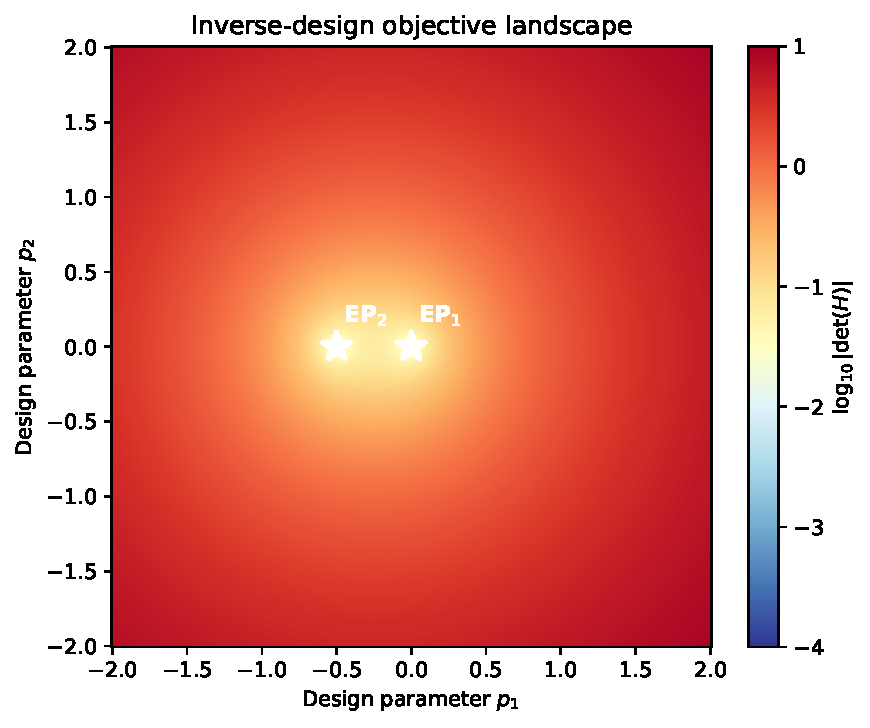
\includegraphics[width=0.6\linewidth]{figures/fig_f19_inverse_design.pdf}
 \caption{Inverse-design objective landscape $\log_{10}|\det H|$ in a
 two-parameter space. The two exceptional points (white stars) appear
 as deep minima where $\det H \to 0$. Gradient-based optimizers must
 navigate this non-convex landscape; adjoint sensitivity formulas from
 QNM perturbation theory provide the required gradients.}
 \label{fig:inverse-design}
\end{figure}

\begin{itemize}
 \item \textbf{EP targeting:} the EP is a codimension-2 degeneracy in
 parameter space; designing a structure that hits an EP at a target
 frequency requires simultaneous tuning of two real parameters.
 \item \textbf{Topological constraints:} enforcing a topological
 invariant (Chern number, winding number, BIC charge) during
 optimization requires discrete-valued objective functions, which
 are not differentiable.
 \item \textbf{Physical realizability:} optimized permittivity
 profiles must satisfy the Kramers--Kronig relations
 (Chapter~\ref{ch:loss-gain-dispersion}), and the gain/loss
 distribution must be achievable with a practical pump geometry.
\end{itemize}

\paragraph{Adjoint sensitivity for non-Hermitian objectives.}
The key technical ingredient for gradient-based inverse design is the
adjoint sensitivity: the derivative of an objective function $\mathcal{F}$
with respect to a material parameter $p$ (e.g., a pixel of $\epsr$).
For a Hermitian system, the adjoint field is the standard conjugate
field. For a non-Hermitian system, the adjoint field must be computed
from the \emph{left} eigenvector or the adjoint Green function, which
introduces the biorthogonal framework of Chapter~\ref{ch:qnm} into the
optimization loop.

For a nondispersive scalar perturbation, the leading sensitivity of a
QNM eigenfrequency $\tilde{\omega}_m$ to a local perturbation
$\delta\epsr(\rr)$ has the schematic form
\begin{equation}
 \frac{\partial\tilde{\omega}_m}{\partial\epsr(\rr)}
 = -\frac{\tilde{\omega}_m}{2}
 \frac{\tilde{\EE}_m(\rr) \cdot \tilde{\EE}_m(\rr)}
 {\langle\tilde{\EE}_m | \epsr | \tilde{\EE}_m\rangle_{\mathrm{bi}}},
 \label{eq:qnm-sensitivity}
\end{equation}
where the denominator represents the appropriate PML-regularized QNM
normalization of Chapter~\ref{ch:qnm}; dispersive, anisotropic, or
magnetic media require the corresponding generalized bilinear form.
This formula is the non-Hermitian generalisation of standard cavity
perturbation theory and provides an efficient route to gradient
computation: one adjoint solve per objective, regardless of the number
of design parameters.

\paragraph{Multi-objective design: EP + topology + noise.}
The most ambitious inverse-design target combines an EP at a specified
frequency, a topological invariant of a given value, and a noise figure
below a threshold. This is a multi-objective, mixed-integer,
Kramers--Kronig-constrained optimization problem that lies beyond
current methods. Developing efficient algorithms for this class of
problems would have immediate practical impact on the design of EP
sensors, topological lasers, and non-Hermitian metasurfaces.


%% ================================================================
\section{Energy, entropy, and thermodynamics}
\label{sec:thermodynamics}

The auxiliary-field construction of
Chapter~\ref{ch:loss-gain-dispersion} shows how to define a conserved
energy for the full field--matter system, even in the presence of
dispersion and dissipation. This construction embeds the non-Hermitian
Maxwell problem into a larger Hermitian system, where standard
thermodynamic concepts (entropy, temperature, free energy) are
well defined.

Whether this embedding can be used to define meaningful thermodynamic
quantities for the non-Hermitian photonic subsystem, and which
quantities remain subsystem-dependent bookkeeping choices, is an
intriguing open question. Specific directions
include:
\begin{itemize}
 \item Defining an entropy production rate for a non-Hermitian
 photonic mode in terms of the energy flow into the auxiliary
 (matter) degrees of freedom.
 \item Connecting the Petermann factor to a thermodynamic cost of
 maintaining a non-orthogonal mode structure.
 \item Establishing fluctuation--dissipation relations for
 non-Hermitian photonic systems that go beyond the standard
 equilibrium results.
\end{itemize}


%% ================================================================
\section{Beyond photonics}
\label{sec:beyond-photonics}

The mathematical framework developed in this book---complex eigenvalues,
biorthogonality, exceptional points, point-gap topology, the skin
effect---applies to any wave system with gain, loss, or non-reciprocity.
Active research frontiers include:

\paragraph{Acoustics and mechanics.}
Coupled acoustic resonators with active feedback and metamaterial
lattices with programmed damping provide macroscopic platforms where
non-Hermitian topology can be tested with tabletop experiments. The
slower wave speeds and larger wavelengths make spatial measurements
easier than in photonics.

\paragraph{Electronics.}
Non-Hermitian circuit lattices (topolectric circuits) with resistive
and reactive elements can realize non-Hermitian tight-binding models
with high controllability. The skin effect, point-gap topology, and
higher-order corner modes have all been observed in electronic circuits.

\paragraph{Cold atoms and condensates.}
Atomic gases with controlled loss (via resonant light or atom removal)
and effective non-Hermitian band structures provide a quantum platform
where the interplay of non-Hermiticity and interactions can be studied
in a controllable setting.

\paragraph{Condensed matter.}
Quasiparticle lifetimes in correlated electron systems generate effective
non-Hermitian self-energies. Point-gap topology and non-Hermitian
self-energy effects have been proposed as possible ingredients in
anomalous surface responses of certain topological semimetals, although
their direct relation to the skin effect in electronic materials remains
subtle.


%% ================================================================
\section{Toward a Maxwell-first synthesis}
\label{sec:maxwell-synthesis}

This monograph has consistently derived non-Hermitian phenomena from the
Maxwell equations rather than postulating them from finite-dimensional
models. Several directions remain where a Maxwell-first approach could
sharpen the understanding:

\paragraph{Topological classification of Maxwell systems.}
The 38-fold classification of non-Hermitian topological phases
(Chapter~\ref{ch:complex-bands}) was developed for tight-binding
Hamiltonians. Lifting it to the continuous Maxwell operator---with its
vector nature, gauge redundancy, and frequency-dependent material
response---is an open problem that could reveal new topological phases
unique to electromagnetism.

The vector nature is the most immediate obstacle: the Maxwell operator
acts on six-component fields $(\EE, \HH)$, not on scalar wave functions.
The polarization degree of freedom couples to the spatial structure
through the boundary conditions and the dielectric tensor, creating a
richer symmetry landscape than the scalar case. For example, a photonic
crystal with time-reversal symmetry and $C_4$ spatial symmetry can
support polarization-dependent topological phases where the TE and TM
sectors have different topological invariants---a situation that has no
analogue in electronic systems where spin--orbit coupling mixes the
spin channels.

\paragraph{Unified energy--topology--noise framework.}
The conserved energy (Chapter~\ref{ch:loss-gain-dispersion}), the
topological invariants (Chapters~\ref{ch:berry-maxwell}--\ref{ch:bbc-rebuilt}),
and the noise limits (Chapter~\ref{ch:devices}) are currently treated as
separate aspects of non-Hermitian photonics. A unified framework that
connects energy conservation, topological robustness, and noise bounds
would be a major theoretical advance---and one that can
only be formulated at the Maxwell level, where all three ingredients
coexist naturally.

A hint of such a connection comes from the Petermann factor: it appears
both as a noise amplification factor (Chapter~\ref{ch:qnm}) and as a
measure of the non-orthogonality of the eigenmodes. Near an EP, the
Petermann factor diverges, the topological charge of the EP is
non-trivial, and the energy stored in the mode becomes anomalously
large relative to the input power. Whether these three divergences are
different facets of a single geometric--thermodynamic quantity---perhaps
a non-Hermitian analogue of the Fisher information metric---is a
compelling open question.

\paragraph{A constrained optimisation perspective.}
The unification problem can be cast as a constrained optimisation over
the design space of non-Hermitian photonic structures. Let
$\mathbf{p}$ denote the design parameters (geometry, material
composition, gain--loss distribution). A device design must
simultaneously satisfy:
\begin{enumerate}
 \item \emph{Topological robustness}: the topological invariant
 $\nu(\mathbf{p})$ (Chern number, winding number, or BIC charge) must
 take a specified integer value.
 \item \emph{Noise bounds}: the Petermann factor
 $K(\mathbf{p})$ must remain below a threshold set by the
 application-level signal-to-noise requirement.
 \item \emph{Gain saturation}: the steady-state intensity
 $I_{\mathrm{ss}}(\mathbf{p})$ must lie within the linear regime
 $I_{\mathrm{ss}} < I_{\mathrm{sat}}$ for the linear non-Hermitian
 model to be valid.
 \item \emph{Fabrication robustness}: the sensitivity
 $\|\partial\nu/\partial\mathbf{p}\|$ must be small enough that
 fabrication disorder does not close the relevant gap or destroy the
 desired boundary response.
\end{enumerate}
These four constraints define a feasible region in design space. The
open question is whether this feasible region is generically nonempty:
can one simultaneously have strong topological robustness
\emph{and} low noise \emph{and} operate below saturation? The
Petermann-factor divergence at EPs
(Chapter~\ref{ch:exceptional-points}) suggests a fundamental tension
between EP-based enhancement and noise, but it is not known whether
alternative mechanisms---such as symmetry- or topology-guided BICs
(Chapter~\ref{ch:bic-topology})---can improve the tradeoff in practical
devices.

A formal optimisation objective that captures this tension is
\begin{equation}
 \min_{\mathbf{p}} \Bigl\{
 -Q_{\mathrm{topo}}(\mathbf{p})
 + \lambda_1\,K(\mathbf{p})
 + \lambda_2\,\frac{I_{\mathrm{ss}}(\mathbf{p})}{I_{\mathrm{sat}}}
 + \lambda_3\,R_{\mathrm{fab}}(\mathbf{p})
 \Bigr\},
 \label{eq:unified-objective}
\end{equation}
where $Q_{\mathrm{topo}}$ is a topological quality metric (e.g.\ the
bulk or point gap supporting the invariant), $K$ is the Petermann factor,
$I_{\mathrm{ss}}/I_{\mathrm{sat}}$ measures the proximity to gain
saturation, $R_{\mathrm{fab}}$ is a fabrication-sensitivity measure, and
$\lambda_i$ are Lagrange-like weights. Solving this optimisation
requires the adjoint sensitivity formulas of
Section~\ref{sec:inverse-design}---themselves an open problem for
non-Hermitian objectives, where the adjoint operator is not the
Hermitian conjugate but the biorthogonal partner.

\paragraph{Stable invariants for nonlinear Maxwell operators.}
The deepest mathematical question in this programme is whether
topological invariants can be defined for nonlinear, noisy Maxwell
operators. The current classification
(Chapter~\ref{ch:complex-bands}) assumes a linear Bloch Hamiltonian;
gain saturation (Chapter~\ref{ch:loss-gain-dispersion}) makes the
effective permittivity intensity-dependent, so the Hamiltonian itself
depends on the solution. Whether a meaningful topological invariant
survives in this self-consistent regime---and whether it can be computed
from a linearised operator around the steady state---is unknown.
Partial answers exist for specific models (e.g.\ the nonlinear SSH
model with Kerr coupling~\cite{hill2026exceptional}), but a general
theory for continuous Maxwell systems with dispersive, nonlinear,
and noisy materials remains an open frontier.

\paragraph{From Maxwell to field theory.}
The Maxwell operator in a periodic non-Hermitian medium is formally a
non-self-adjoint elliptic operator on a fibre bundle over the Brillouin
torus. The topological invariants of Chapters~\ref{ch:berry-maxwell}
through~\ref{ch:bbc-rebuilt} are characteristic classes of this bundle.
A field-theoretic formulation---using the language of differential
geometry and gauge theory---could clarify which invariants survive for
continuous, dispersive Maxwell operators. One possible starting point is
a non-Hermitian analogue of index theorems that relate boundary
responses to a topological index computed from the bulk Maxwell
operator.
Whether such a theorem exists for non-self-adjoint operators---and
whether it can be proven with the regularity available for Maxwell
systems with dispersive media---is a deep mathematical question at the
intersection of spectral theory, differential geometry, and photonics.

\begin{takeaway}[A field in motion]
Non-Hermitian photonics has grown quickly from a mathematical theme into
an experimental and theoretical field. Combining Maxwell's equations with
non-Hermitian spectral theory gives a disciplined way to pose its open
problems, from nonlinear topology to the thermodynamics of
non-orthogonal modes. The tools assembled here---the Maxwell eigenproblem,
the biorthogonal expansion, the GBZ, and topological charge---are starting
points for that next stage.
\end{takeaway}


% ── Appendices ──────────────────────────────────────────────
\appendix
\chapter{Vector Calculus and Maxwell Notation}
\label{app:vector}

This appendix collects the vector-calculus identities, integration
formulas, and notational conventions used throughout the book. All
results are stated for three-dimensional space with Cartesian, or
where noted, curvilinear coordinates.


%% ================================================================
\section{Curl identities}
\label{sec:curl-identities}

The following identities are used repeatedly in the derivation of
Maxwell inner products and self-adjointness conditions.

\paragraph{Double curl.}
\begin{equation}
 \curl(\curl\FF) = \grad(\divg\FF) - \nabla^2\FF.
 \label{eq:double-curl}
\end{equation}

\paragraph{Curl of a product.}
\begin{equation}
 \curl(f\,\FF) = f\,\curl\FF + (\grad f)\times\FF.
 \label{eq:curl-product}
\end{equation}

\paragraph{Divergence of a cross product.}
\begin{equation}
 \divg(\FF \times \GG) = \GG\cdot\curl\FF - \FF\cdot\curl\GG.
 \label{eq:div-cross}
\end{equation}
This identity is the vector-calculus engine behind every
integration-by-parts argument in this book: integrating both sides over
a volume and applying the divergence theorem converts a volume integral
of curls into a surface integral.


%% ================================================================
\section{Integration by parts for curl operators}
\label{sec:integration-by-parts}

Let $\FF$ and $\GG$ be smooth vector fields on a domain $\Omega$ with
boundary $\partial\Omega$ and outward normal $\nn$. Then
\begin{equation}
 \int_\Omega \GG\cdot\curl\FF\;\dd V
 = \int_\Omega \FF\cdot\curl\GG\;\dd V
 + \oint_{\partial\Omega}(\FF\times\GG)\cdot\nn\;\dd S.
 \label{eq:curl-ibp-app}
\end{equation}
This is the fundamental self-adjointness identity for the curl operator.
Setting $\FF = \EE$ and $\GG = \mur^{-1}\curl\EE$ (or the
corresponding magnetic formulation) and requiring the surface integral
to vanish yields the Hermiticity condition for the Maxwell curl--curl
operator (Chapter~\ref{ch:energy-inner}).

\subsection{Boundary conditions that kill the surface term}
\label{ssec:vanishing-surface}

The surface integral in~\eqref{eq:curl-ibp-app} vanishes if any of the
following conditions hold on $\partial\Omega$:
\begin{enumerate}
 \item \textbf{Perfect electric conductor (PEC):}
 $\nn\times\EE = 0$ on $\partial\Omega$.
 \item \textbf{Perfect magnetic conductor (PMC):}
 $\nn\times\HH = 0$ on $\partial\Omega$.
 \item \textbf{Periodic boundary conditions:}
 $\FF$ and $\GG$ satisfy Bloch periodicity on opposite faces, so the
 contributions cancel pairwise.
 \item \textbf{Fields decay sufficiently fast:}
 for an unbounded domain, if $|\FF|$ and $|\GG|$ decay faster than
 $1/r$ as $r \to \infty$, the surface integral at infinity vanishes.
\end{enumerate}
When the surface term does \emph{not} vanish---as for outgoing radiation
boundary conditions (Silver--M\"uller condition) or for modes with
$|\FF| \sim e^{+\Im k\,r}$---the curl--curl operator is no longer
self-adjoint, and the system is non-Hermitian
(Chapter~\ref{ch:boundaries}).


%% ================================================================
\section{The divergence theorem and Poynting's theorem}
\label{sec:divergence-poynting}

The divergence theorem relates a volume integral of a divergence to a
surface integral:
\begin{equation}
 \int_\Omega \divg\FF\;\dd V
 = \oint_{\partial\Omega} \FF\cdot\nn\;\dd S.
 \label{eq:divergence-theorem}
\end{equation}
Applying this to the Poynting vector
$\SS = \EE\times\HH$ gives the integral form of Poynting's theorem:
\begin{equation}
 -\pdv{}{t}\int_\Omega u\;\dd V
 = \oint_{\partial\Omega} \SS\cdot\nn\;\dd S
 + \int_\Omega \sigma\,|\EE|^2\;\dd V,
 \label{eq:poynting-integral}
\end{equation}
where $u$ is the electromagnetic energy density and $\sigma$ is the
conductivity (representing ohmic loss).


%% ================================================================
\section{Bloch-periodic boundary terms}
\label{sec:bloch-boundary}

For a photonic crystal with lattice vectors $\aa_1, \aa_2, \aa_3$ and
Bloch wave vector $\kk$, the fields satisfy
\begin{equation}
 \FF(\rr + \aa_j) = e^{i\kk\cdot\aa_j}\,\FF(\rr).
 \label{eq:bloch-bc}
\end{equation}
On a unit cell $\Omega_{\mathrm{cell}}$ with faces $S_j^+$ and $S_j^-$
related by $S_j^+ = S_j^- + \aa_j$, the surface integral
in~\eqref{eq:curl-ibp-app} cancels pairwise when the two fields belong
to compatible Bloch sectors. For example, if both fields carry the same
real Bloch wave vector and the inner product uses the usual conjugation,
or if an unconjugated bilinear form pairs $\kk$ with $-\kk$, the two
opposite faces contribute
\begin{equation}
 \int_{S_j^+}(\FF\times\GG)\cdot\nn\;\dd S
 + \int_{S_j^-}(\FF\times\GG)\cdot\nn\;\dd S = 0 .
 \label{eq:bloch-surface-cancel}
\end{equation}
The cancellation is not simply the algebraic difference
$e^{i\kk\cdot\aa_j}-e^{-i\kk\cdot\aa_j}$; it also uses the opposite
orientations of the outward normals and the adjoint boundary condition.
For real $\kk$ in a lossless periodic medium this gives the usual
self-adjoint Bloch Maxwell problem. For complex $\kk$, as in non-Bloch
or GBZ constructions, the operator is generally non-self-adjoint and
one must pair right and adjoint Bloch sectors explicitly.


%% ================================================================
\section{Silver--M\"uller radiation condition}
\label{sec:silver-muller}

For an open scatterer in three dimensions, the outgoing-wave condition
at infinity is the Silver--M\"uller condition:
\begin{equation}
 \lim_{r\to\infty} r\,\bigl[
 \hat{\rr}\times(\curl\EE) - ik\,\EE
 \bigr] = 0,
 \label{eq:silver-muller-app}
\end{equation}
uniformly in all directions $\hat{\rr}$. This condition selects
outgoing spherical waves and excludes incoming waves. It is the
mathematical statement of the ``no incoming radiation'' assumption that
makes the scattering problem well posed and the Maxwell operator
non-self-adjoint (Chapter~\ref{ch:boundaries}).


%% ================================================================
\section{Notation conventions}
\label{sec:notation}

\subsection{Time convention}
The time-harmonic convention throughout this book is
$e^{-i\omega t}$. With this choice:
\begin{itemize}
 \item A passive medium has $\Im\epsr > 0$ (absorption).
 \item A gain medium has $\Im\epsr < 0$ (amplification).
 \item A QNM eigenfrequency $\omtil = \omega_r - i\gamma$ with
 $\gamma > 0$ represents a decaying mode.
\end{itemize}

\subsection{Field quantities}
\begin{center}
\begin{tabular}{lll}
\toprule
Symbol & Name & SI Unit \\
\midrule
$\EE$ & Electric field & V/m \\
$\HH$ & Magnetic field & A/m \\
$\DD$ & Electric displacement & C/m$^2$ \\
$\BB$ & Magnetic induction & T \\
$\SS = \EE\times\HH$ & Poynting vector & W/m$^2$ \\
$\epsr$ & Relative permittivity & dimensionless \\
$\mur$ & Relative permeability & dimensionless \\
$\omega$ & Angular frequency & rad/s \\
$\omtil$ & Complex eigenfrequency & rad/s \\
$\kk$ & Wave vector & 1/m \\
$c$ & Speed of light in vacuum & m/s \\
\bottomrule
\end{tabular}
\end{center}

\subsection{Operators and inner products}
\begin{center}
\begin{tabular}{ll}
\toprule
Symbol & Meaning \\
\midrule
$\curl$ & Curl operator \\
$\divg$ & Divergence operator \\
$\grad$ & Gradient operator \\
$\hat{\Theta}$ & Maxwell curl--curl operator \\
$\Smat$ & Scattering matrix \\
$\Tmat$ & Transfer matrix \\
$\langle\cdot|\cdot\rangle$ & Standard (conjugated) inner product \\
$(\cdot,\cdot)$ & Unconjugated bilinear form \\
$\Qfac$ & Quality factor \\
$\wnum$ & Winding number \\
$\PT$ & Parity--time operator \\
\bottomrule
\end{tabular}
\end{center}


%% ================================================================
\section{Electromagnetic reciprocity from vector calculus}
\label{sec:reciprocity-vector}

The Lorentz reciprocity theorem, introduced physically in
Chapter~\ref{ch:energy-inner}, can be derived purely from the vector
calculus identities of this appendix.

\subsection{Statement and proof}
\label{ssec:reciprocity-proof}

Consider two solutions $(\EE_1, \HH_1)$ and $(\EE_2, \HH_2)$ of
Maxwell's equations at the same frequency $\omega$ in a medium with
permittivity tensor $\boldsymbol{\varepsilon}$ and permeability
$\mu_0$. The sources are localised current densities $\JJ_1$ and
$\JJ_2$. Define the \emph{reaction} of field~1 on source~2:
\begin{equation}
 \langle 1, 2 \rangle = \int_V \EE_1 \cdot \JJ_2\;\dd^3 r.
 \label{eq:reaction-app}
\end{equation}
Lorentz reciprocity states that
$\langle 1, 2 \rangle = \langle 2, 1 \rangle$ whenever
$\boldsymbol{\varepsilon} = \boldsymbol{\varepsilon}^\transpose$
(the permittivity tensor is symmetric, not necessarily Hermitian).

\paragraph{Proof.}
Start from the divergence-of-cross-product identity~\eqref{eq:div-cross}:
\begin{equation}
 \nabla \cdot (\EE_1 \times \HH_2 - \EE_2 \times \HH_1)
 = \HH_2 \cdot (\nabla \times \EE_1) - \EE_1 \cdot (\nabla \times \HH_2)
 - \HH_1 \cdot (\nabla \times \EE_2) + \EE_2 \cdot (\nabla \times \HH_1).
 \label{eq:reciprocity-divergence}
\end{equation}
Substituting Maxwell's curl equations
$\nabla \times \EE_j = i\omega\mu_0\HH_j$ and
$\nabla \times \HH_j = -i\omega\boldsymbol{\varepsilon}\EE_j + \JJ_j$
into the right-hand side:
\begin{align}
 \text{RHS} &= i\omega\mu_0\,\HH_2 \cdot \HH_1
 + i\omega\,\EE_1 \cdot \boldsymbol{\varepsilon}\EE_2
 - \EE_1 \cdot \JJ_2
 \notag\\
 &\quad - i\omega\mu_0\,\HH_1 \cdot \HH_2
 - i\omega\,\EE_2 \cdot \boldsymbol{\varepsilon}\EE_1
 + \EE_2 \cdot \JJ_1.
 \label{eq:reciprocity-rhs}
\end{align}
The $\mu_0$ terms cancel. The permittivity terms give
$i\omega(\EE_1 \cdot \boldsymbol{\varepsilon}\EE_2
- \EE_2 \cdot \boldsymbol{\varepsilon}\EE_1)$, which vanishes if and
only if $\boldsymbol{\varepsilon} = \boldsymbol{\varepsilon}^\transpose$.
What remains is
\begin{equation}
 \nabla \cdot (\EE_1 \times \HH_2 - \EE_2 \times \HH_1)
 = \EE_2 \cdot \JJ_1 - \EE_1 \cdot \JJ_2.
 \label{eq:reciprocity-simplified}
\end{equation}
Integrating over a volume $V$ that contains both sources and applying
the divergence theorem, the left-hand side becomes a surface integral
that vanishes when the fields satisfy Silver--M\"uller radiation
conditions at infinity (or when the surface is a PEC boundary):
\begin{equation}
 \oint_{\partial V} (\EE_1 \times \HH_2 - \EE_2 \times \HH_1)
 \cdot \hat{\nn}\;\dd S = 0.
 \label{eq:reciprocity-surface}
\end{equation}
Therefore $\langle 2, 1 \rangle - \langle 1, 2 \rangle = 0$, proving
Lorentz reciprocity.

\subsection{Reciprocity versus Hermiticity}
\label{ssec:reciprocity-vs-hermiticity}

The proof makes clear the distinction emphasised in
Chapter~\ref{ch:energy-inner}: reciprocity requires
$\boldsymbol{\varepsilon}^\transpose = \boldsymbol{\varepsilon}$
(symmetric), while Hermiticity of the Maxwell operator requires
$\boldsymbol{\varepsilon}^\dagger = \boldsymbol{\varepsilon}$
(Hermitian, i.e.\ real for a scalar permittivity). A medium with
complex symmetric $\boldsymbol{\varepsilon}$ (such as a lossy isotropic
dielectric) is reciprocal but not Hermitian. Conversely, a
magneto-optical medium with real antisymmetric off-diagonal elements is
Hermitian (lossless) but not reciprocal.

This distinction is central to non-Hermitian photonics: most passive
non-Hermitian systems (lossy dielectrics, absorbing metasurfaces) are
reciprocal, and reciprocity constrains their scattering matrices and
coupled-mode models. Reciprocity can fail when the material tensor,
temporal modulation, active feedback, or an effective modal reduction
lacks the relevant transpose symmetry. Such non-reciprocal or
asymmetric effective couplings are one route to point-gap winding and
the non-Hermitian skin effect of Chapter~\ref{ch:skin-effect}, although
the precise criterion is spectral rather than simply the presence or
absence of material loss.

\chapter{Non-Normal Linear Algebra}
\label{app:nonnormal}

This appendix collects the linear-algebra results that underpin the
non-Hermitian spectral theory used throughout the book. The central
theme is \emph{non-normality}: a matrix $A$ is normal if
$A A^\dagger = A^\dagger A$; Hermitian, unitary, and skew-Hermitian
matrices are all normal. A non-normal matrix can have a complete set
of eigenvectors, but they are not orthogonal, and the spectral behavior
under perturbation is qualitatively different from the normal case.
Non-Hermitian photonic operators---the Maxwell operator with complex
$\epsr$, the scattering matrix near an EP, the effective Hamiltonian of
a coupled-mode model---are generically non-normal.


%% ================================================================
\section{Left and right eigenvectors}
\label{sec:left-right}

For a matrix $A \in \mathbb{C}^{n \times n}$, the \emph{right
eigenvector} $|r_j\rangle$ and the \emph{left eigenvector}
$\langle l_j|$ associated with eigenvalue $\lambda_j$ satisfy
\begin{equation}
 A\,|r_j\rangle = \lambda_j\,|r_j\rangle, \qquad
 \langle l_j|\,A = \lambda_j\,\langle l_j|.
 \label{eq:left-right-def}
\end{equation}
Equivalently, $\langle l_j|$ is a right eigenvector of $A^\dagger$
with eigenvalue $\lambda_j^*$.

For a normal matrix, left and right eigenvectors coincide (up to
normalization):\ $|l_j\rangle = |r_j\rangle$. For a non-normal matrix,
they differ, and the angle between corresponding left and right
eigenvectors can be arbitrarily small---a situation that has dramatic
physical consequences (enhanced noise, sensitivity to perturbation,
mode non-orthogonality).


%% ================================================================
\section{Biorthogonality}
\label{sec:biorthogonality-app}

If $A$ has $n$ distinct eigenvalues, the left and right eigenvectors
form a \emph{biorthogonal} system:
\begin{equation}
 \langle l_i | r_j \rangle = \delta_{ij}\,N_j,
 \label{eq:biorthogonal}
\end{equation}
where $N_j = \langle l_j | r_j \rangle$ is a nonzero normalization
constant (which is generally complex for non-normal matrices). The
biorthogonal normalization convention sets $N_j = 1$ for all $j$ by
rescaling.

The spectral decomposition of $A$ takes the biorthogonal form
\begin{equation}
 A = \sum_{j=1}^n \lambda_j\,|r_j\rangle\langle l_j|,
 \label{eq:spectral-biorthogonal}
\end{equation}
and the resolvent is
\begin{equation}
 (z - A)^{-1} = \sum_{j=1}^n \frac{|r_j\rangle\langle l_j|}
 {z - \lambda_j}.
 \label{eq:resolvent-biorthogonal}
\end{equation}
These formulas generalize the Hermitian spectral theorem to the
non-normal case. They are the mathematical foundation for the
quasinormal-mode expansion (Chapter~\ref{ch:qnm}) and the
biorthogonal Berry phase (Chapter~\ref{ch:complex-bands}).


%% ================================================================
\section{Jordan chains and defective eigenvalues}
\label{sec:jordan-app}

When two or more eigenvalues coalesce, the eigenvectors may also
coalesce, producing a \emph{defective} eigenvalue---an exceptional
point (Chapter~\ref{ch:exceptional-points}).

\subsection{Jordan normal form}
\label{ssec:jordan-form}

At a defective eigenvalue $\lambda_0$ of algebraic multiplicity $m$ and
geometric multiplicity $g < m$, the matrix $A$ cannot be diagonalized.
Instead, the relevant block of the Jordan normal form is
\begin{equation}
 J_m(\lambda_0) = \begin{pmatrix}
 \lambda_0 & 1 & 0 & \cdots & 0 \\
 0 & \lambda_0 & 1 & \cdots & 0 \\
 \vdots & & \ddots & \ddots & \vdots \\
 0 & \cdots & 0 & \lambda_0 & 1 \\
 0 & \cdots & 0 & 0 & \lambda_0
 \end{pmatrix}
 \in \mathbb{C}^{m \times m}.
 \label{eq:jordan-block-app}
\end{equation}

\subsection{Generalized eigenvectors}
\label{ssec:generalized-evecs}

The Jordan chain associated with $J_m(\lambda_0)$ consists of vectors
$|v_0\rangle, |v_1\rangle, \ldots, |v_{m-1}\rangle$ satisfying
\begin{equation}
 (A - \lambda_0)\,|v_0\rangle = 0, \qquad
 (A - \lambda_0)\,|v_p\rangle = |v_{p-1}\rangle,
 \quad p = 1, \ldots, m-1.
 \label{eq:jordan-chain-app}
\end{equation}
Only $|v_0\rangle$ is a true eigenvector; the higher-order vectors
$|v_p\rangle$ are \emph{generalized eigenvectors}. At a second-order
EP ($m = 2$), there is one eigenvector and one generalized eigenvector;
the biorthogonal decomposition~\eqref{eq:spectral-biorthogonal} breaks
down and must be replaced by the Jordan decomposition.

\subsection{Resolvent near an EP}
\label{ssec:resolvent-ep}

Near a second-order EP at $\lambda_0$, the resolvent has a
second-order pole:
\begin{equation}
 (z - A)^{-1} \approx
 \frac{|v_1\rangle\langle w_0|}{(z - \lambda_0)^2}
 + \frac{|v_0\rangle\langle w_0| + |v_1\rangle\langle w_1|}
 {z - \lambda_0}
 + \text{regular},
 \label{eq:resolvent-ep}
\end{equation}
where $\langle w_0|$ and $\langle w_1|$ are the left Jordan-chain
vectors. The double pole produces algebraic (rather than exponential)
temporal growth---the hallmark of an EP in time-domain experiments and
the origin of the enhanced transient response.


%% ================================================================
\section{Petermann factor and excess noise}
\label{sec:petermann-app}

The Petermann factor quantifies the enhancement of spontaneous emission
(and, more generally, noise) in a non-normal system. For a mode with
right eigenvector $|r_j\rangle$ and left eigenvector $\langle l_j|$,
the Petermann factor is
\begin{equation}
 K_j = \frac{\langle r_j | r_j \rangle \;\langle l_j | l_j \rangle}
 {|\langle l_j | r_j \rangle|^2} \ge 1,
 \label{eq:petermann-def}
\end{equation}
with equality if and only if $|l_j\rangle = |r_j\rangle$ (the normal
case).

\subsection{Physical interpretation}
\label{ssec:petermann-physics-app}

In a laser, spontaneous emission couples to the lasing mode with an
amplitude proportional to $|\langle l_j | r_j \rangle|^{-1}$. When
the left and right eigenvectors are nearly orthogonal (as happens near
an EP), this coupling is enhanced, broadening the laser linewidth by
the factor $K_j$:
\begin{equation}
 \Delta\nu = K_j\,\Delta\nu_{\mathrm{ST}},
 \label{eq:petermann-linewidth-app}
\end{equation}
where $\Delta\nu_{\mathrm{ST}}$ is the Schawlow--Townes linewidth.

\subsection{Scaling near an EP}
\label{ssec:petermann-ep}

Near a second-order EP, the overlap $\langle l_j | r_j \rangle$
vanishes as $\sqrt{\epsilon}$ where $\epsilon$ is the distance from
the EP in parameter space. Therefore the Petermann factor diverges as
\begin{equation}
 K_j \sim \frac{1}{\epsilon}
 \label{eq:petermann-ep-scaling}
\end{equation}
near the EP. In common equal-resource sensing models, the associated
noise growth can offset the enhanced frequency splitting
$\Delta\omega \sim \sqrt{\epsilon}$ in a signal-to-noise proxy, as
discussed in Chapter~\ref{ch:devices}. The quantitative cancellation is
not universal; it depends on the measurement protocol, noise channels,
and normalization of the sensor response.

For an $n$-th order EP, analogous power-law divergences appear, but the
resulting precision bound must be evaluated from the full noise model
rather than inferred from the eigenvalue splitting alone.


%% ================================================================
\section{Phase rigidity}
\label{sec:phase-rigidity}

The \emph{phase rigidity} of a mode is the inverse of the Petermann
factor:
\begin{equation}
 r_j = \frac{|\langle l_j | r_j \rangle|^2}
 {\langle r_j | r_j \rangle \;\langle l_j | l_j \rangle}
 = K_j^{-1} \in [0, 1].
 \label{eq:phase-rigidity-def}
\end{equation}
A phase rigidity of $r_j = 1$ indicates a normal (Hermitian-like) mode;
$r_j \to 0$ indicates an EP where the mode becomes maximally
non-orthogonal.


%% ================================================================
\section{Pseudospectra}
\label{sec:pseudospectra}

The spectrum of a non-normal matrix can be misleading: eigenvalues may
be highly sensitive to perturbations even when they are well separated.
The \emph{$\epsilon$-pseudospectrum} quantifies this sensitivity.

\subsection{Definition}
\label{ssec:pseudospec-def}

The $\epsilon$-pseudospectrum of $A$ is the set of complex numbers
$z$ such that $z$ is an eigenvalue of $A + E$ for some perturbation
$\|E\| \le \epsilon$:
\begin{equation}
 \sigma_\epsilon(A) = \{z \in \mathbb{C} :
 \|(z - A)^{-1}\| \ge \epsilon^{-1}\}.
 \label{eq:pseudospectrum}
\end{equation}
For a normal matrix, the $\epsilon$-pseudospectrum is the union of
$\epsilon$-disks around each eigenvalue. For a non-normal matrix, the
pseudospectrum can extend far beyond these disks, indicating that
eigenvalues can move large distances under small perturbations.

\subsection{Physical relevance}
\label{ssec:pseudospec-physics}

Pseudospectra are relevant whenever the system is subject to
perturbations---fabrication disorder, environmental fluctuations,
or numerical discretization errors. For a photonic system operating
near an EP, the pseudospectrum extends over a large region of the
complex frequency plane, meaning that the eigenfrequencies are
effectively unpredictable to within a band set by the perturbation
strength. This is the spectral manifestation of the Petermann-factor
divergence and the reason why EP-based devices require careful
noise analysis (Chapter~\ref{ch:devices}).


%% ================================================================
\section{Matrix functions and the non-Hermitian exponential}
\label{sec:matrix-exp}

The time evolution of a system governed by $i\,\partial_t |\psi\rangle
= A\,|\psi\rangle$ is
\begin{equation}
 |\psi(t)\rangle = e^{-iAt}\,|\psi(0)\rangle.
 \label{eq:time-evolution}
\end{equation}
For a normal $A$, the evolution is a superposition of oscillating and
decaying exponentials, and $\|e^{-iAt}\|$ is controlled by the largest
imaginary part of the eigenvalues. For a non-normal $A$, the situation
is richer: the Jordan chain at a defective eigenvalue contributes
\emph{polynomial} growth factors
\begin{equation}
 e^{-iJ_m(\lambda_0)t} = e^{-i\lambda_0 t}
 \begin{pmatrix}
 1 & -it & (-it)^2/2! & \cdots \\
 0 & 1 & -it & \cdots \\
 \vdots & & \ddots & \ddots \\
 0 & \cdots & 0 & 1
 \end{pmatrix},
 \label{eq:jordan-exponential}
\end{equation}
so the amplitude can grow as $t^{m-1}$ even when the eigenvalue has
a negative imaginary part (i.e., the mode is formally decaying). This
\emph{transient growth} is a hallmark of non-normality and is
observable as a power-law ring-up before the eventual exponential
decay in photonic resonators near an EP.

Additionally, even in the absence of defective eigenvalues, a highly
non-normal matrix can produce large transient growth---the so-called
\emph{pseudospectral} transient, where the norm $\|e^{-iAt}\|$ overshoots
its long-time asymptote by a factor that can be estimated from the
pseudospectrum. This effect is important for FDTD simulations of
non-Hermitian photonic systems (Section~\ref{sec:fdtd}), where a
transient overshoot can trigger numerical instability before the
physical decay sets in.


%% ================================================================
\section{Examples}
\label{sec:nonnormal-examples}

\subsection{Jordan decomposition of a $2\times 2$ defective matrix}
\label{ssec:jordan-2x2}

The simplest defective matrix arises at an exceptional point of a
$2\times 2$ non-Hermitian Hamiltonian. Consider
\begin{equation}
 A = \begin{pmatrix} \lambda_0 & 1 \\ 0 & \lambda_0 \end{pmatrix},
 \label{eq:jordan-2x2-example}
\end{equation}
which is already in Jordan normal form $J_2(\lambda_0)$. This matrix
has a single eigenvalue $\lambda_0$ with algebraic multiplicity~2 but
geometric multiplicity~1: there is only one linearly independent
eigenvector, $\mathbf{v}_1 = (1, 0)^\transpose$. The second vector in
the Jordan chain is the \emph{generalized eigenvector} $\mathbf{v}_2$
satisfying $(A - \lambda_0 I)\mathbf{v}_2 = \mathbf{v}_1$, which gives
$\mathbf{v}_2 = (0, 1)^\transpose$.

The time evolution is
\begin{equation}
 e^{-iAt} = e^{-i\lambda_0 t}
 \begin{pmatrix} 1 & -it \\ 0 & 1 \end{pmatrix}.
 \label{eq:jordan-2x2-evolution}
\end{equation}
Even if $\Im\lambda_0 < 0$ (the mode decays), the off-diagonal element
$-it$ grows linearly before the exponential decay dominates. The
maximum of $\|e^{-iAt}\|$ over time occurs at
$t^* \sim 1/|\Im\lambda_0|$, with an envelope of order
$1/(e|\Im\lambda_0|)$ before constant prefactors from the chosen norm
are included. The transient amplification therefore diverges as the
eigenvalue approaches the real axis, but the numerical prefactor is
norm dependent.

\subsection{Schur decomposition and its use}
\label{ssec:schur-decomp}

Every square matrix $A$ admits a Schur decomposition $A = Q T Q^{-1}$,
where $Q$ is unitary and $T$ is upper triangular with the eigenvalues on
the diagonal. Unlike the Jordan form, which requires exact knowledge of
the eigenvector structure, the Schur form is numerically stable and can
be computed by standard algorithms (QR iteration).

The Schur form reveals the \emph{departure from normality}
$\Delta_F = \|A\|_F^2 - \sum_i |\lambda_i|^2$, where $\|\cdot\|_F$
is the Frobenius norm. For a normal matrix, $\Delta_F = 0$ (the Schur
form is diagonal); for a non-normal matrix, $\Delta_F > 0$ measures the
energy stored in the off-diagonal elements of $T$, which is the source
of transient amplification and pseudospectral broadening.

For photonic applications, the Schur decomposition is preferable to the
Jordan form for three reasons. First, it is numerically robust: no
special treatment is needed for nearly defective matrices. Second, the
unitary factor $Q$ preserves norms, making it easy to compute
$\|e^{-iAt}\|$ from $\|e^{-iTt}\|$. Third, the off-diagonal elements
of $T$ give a direct and intuitive measure of the non-Hermitian coupling
between modes---elements that are absent in normal systems.

\subsection{Kreiss constant and transient bounds}
\label{ssec:kreiss}

The maximum transient growth $\sup_{t \ge 0}\|e^{-iAt}\|$ can be
bounded using the Kreiss matrix theorem. The \emph{Kreiss constant}
\begin{equation}
 \mathcal{K}(A) = \sup_{\Im z > \alpha_{\max}}
 (\Im z - \alpha_{\max})\,\|(z - A)^{-1}\|,
 \label{eq:kreiss-constant}
\end{equation}
where $\alpha_{\max} = \max_i \Im\lambda_i$ is the maximum eigenvalue
imaginary part, satisfies the bounds
\begin{equation}
 \mathcal{K}(A) \le \sup_{t \ge 0} \|e^{-iAt}\|\,e^{\alpha_{\max}t}
 \le e\,n\,\mathcal{K}(A),
 \label{eq:kreiss-bounds}
\end{equation}
where $n$ is the matrix dimension. The Kreiss constant is computable
from the resolvent norm (essentially the pseudospectrum) and provides
a practical upper bound on the transient growth without requiring
explicit time integration.

For the $2\times 2$ PT-symmetric Hamiltonian near the EP
($\gamma/\kappa = 0.99$), the Kreiss constant is
$\mathcal{K} \approx 7.1$, consistent with the transient amplification
factor of $7.09$ computed directly from~\eqref{eq:transient-max}. For
larger photonic systems, the Kreiss constant can be estimated from the
pseudospectrum using standard numerical linear algebra packages.

\subsection{Non-normal perturbation theory}
\label{ssec:nonnormal-perturbation}

For a non-normal matrix $A$ with a defective eigenvalue $\lambda_0$ of
algebraic multiplicity $m$, a generic perturbation $\epsilon B$ splits
the eigenvalue into $m$ branches:
\begin{equation}
 \lambda_j(\epsilon) = \lambda_0
 + \epsilon^{1/m}\,c_j + O(\epsilon^{2/m}),
 \qquad j = 1, \ldots, m,
 \label{eq:puiseux-series}
\end{equation}
where $c_j$ are the $m$-th roots of a coupling coefficient that depends
on the perturbation matrix $B$ and the Jordan chain vectors. This
Puiseux series expansion is the mathematical basis for the enhanced
spectral response at exceptional points: a perturbation of order
$\epsilon$ produces an eigenvalue splitting of order
$\epsilon^{1/m}$, which for small $\epsilon$ is much larger than the
linear splitting $\sim\epsilon$ of a non-defective eigenvalue.

However, the Puiseux expansion is \emph{not} isotropic in the
perturbation: the coefficient $c_j$ depends on the \emph{direction} of
the perturbation in parameter space, not just its magnitude. For
certain perturbation directions (those orthogonal to the Jordan chain
coupling), the splitting can be much smaller than $\epsilon^{1/m}$ or
even vanish. This anisotropy is important for EP-based sensing: the
enhanced response occurs only for perturbations that couple to the
Jordan chain, not for arbitrary environmental noise.

\chapter{Transfer Matrices and Scattering}
\label{app:transfer}

This appendix develops the one-dimensional transfer-matrix formalism
that appears in Chapters~\ref{ch:pt-symmetric}, \ref{ch:poles-zeros},
and~\ref{ch:bbc-rebuilt}. The results are exact for multilayer
dielectric stacks with complex permittivity and provide the
computational backbone for many of the non-Hermitian scattering
calculations in this book.


%% ================================================================
\section{Single-layer transfer matrix}
\label{sec:single-layer}

Consider a homogeneous layer of thickness $d$, refractive index
$n = n_r + i n_i$, at normal incidence. The electric field at
position $x$ is a superposition of forward and backward waves:
\begin{equation}
 E(x) = A\,e^{ink_0 x} + B\,e^{-ink_0 x},
 \label{eq:field-ab}
\end{equation}
where $k_0 = \omega/c$. The transfer matrix $M$ relates the field
amplitudes at the left face ($x = 0$) to those at the right face
($x = d$):
\begin{equation}
 \begin{pmatrix} A \\ B \end{pmatrix}_{\!x=d}
 = M\,
 \begin{pmatrix} A \\ B \end{pmatrix}_{\!x=0},
 \qquad
 M = \begin{pmatrix}
 e^{ink_0 d} & 0 \\
 0 & e^{-ink_0 d}
 \end{pmatrix}.
 \label{eq:propagation-matrix}
\end{equation}
At an interface between media with indices $n_1$ and $n_2$, the
interface matrix is
\begin{equation}
 I_{12} = \frac{1}{2n_2}\begin{pmatrix}
 n_2 + n_1 & n_2 - n_1 \\
 n_2 - n_1 & n_2 + n_1
 \end{pmatrix}.
 \label{eq:interface-matrix}
\end{equation}
The total transfer matrix for a multilayer stack is the ordered product
of propagation and interface matrices:
\begin{equation}
 \Tmat = I_{N,\mathrm{out}} \cdot M_N \cdots I_{23} \cdot M_2
 \cdot I_{12} \cdot M_1.
 \label{eq:total-transfer}
\end{equation}


%% ================================================================
\section{Scattering matrix from the transfer matrix}
\label{sec:transfer-to-scatter}

The $2 \times 2$ scattering matrix $\Smat$ relates the outgoing
amplitudes to the incoming amplitudes:
\begin{equation}
 \begin{pmatrix} B_L \\ A_R \end{pmatrix}
 = \Smat
 \begin{pmatrix} A_L \\ B_R \end{pmatrix}
 = \begin{pmatrix}
 r_L & t' \\
 t & r_R
 \end{pmatrix}
 \begin{pmatrix} A_L \\ B_R \end{pmatrix},
 \label{eq:smat-def}
\end{equation}
where $r_L$, $r_R$ are the reflection coefficients from the left and
right, and $t$, $t'$ are the transmission coefficients. The conversion
from the transfer matrix $\Tmat = \bigl(\begin{smallmatrix}
T_{11} & T_{12} \\ T_{21} & T_{22} \end{smallmatrix}\bigr)$ is
\begin{equation}
 t = \frac{1}{T_{22}}, \qquad
 t' = \frac{\det\Tmat}{T_{22}}, \qquad
 r_L = -\frac{T_{21}}{T_{22}}, \qquad
 r_R = \frac{T_{12}}{T_{22}}.
 \label{eq:transfer-to-scatter}
\end{equation}

For a reciprocal medium (symmetric $\epsr$ tensor), $t = t'$ and
$\det\Tmat = 1$. For a non-reciprocal medium, $t \neq t'$ in general.


%% ================================================================
\section{$\PT$-symmetric transfer matrices}
\label{sec:pt-transfer-app}

A one-dimensional structure with $\PT$ symmetry satisfies
$n(x) = n^*(-x)$. For a multilayer consisting of a loss layer
(index $n_0 + i\kappa$, thickness $d$) followed by a gain layer
(index $n_0 - i\kappa$, thickness $d$), the unit-cell transfer
matrix is
\begin{equation}
 \Tmat_{\mathrm{cell}} = M_{\mathrm{gain}} \cdot I \cdot
 M_{\mathrm{loss}}.
 \label{eq:pt-unit-cell}
\end{equation}
The $\PT$ condition imposes the constraint
\begin{equation}
 \sigma_x\,\Tmat_{\mathrm{cell}}^*\,\sigma_x = \Tmat_{\mathrm{cell}},
 \qquad \sigma_x = \begin{pmatrix} 0 & 1 \\ 1 & 0 \end{pmatrix},
 \label{eq:pt-transfer-constraint}
\end{equation}
which ensures that $T_{11} = T_{22}^*$ and $T_{12} = T_{21}^*$. For
the scattering matrix, this gives
\begin{equation}
 |t|^2 - |r_L|\,|r_R| = 1
 \quad\text{(exact $\PT$ relation)},
 \label{eq:pt-unitarity}
\end{equation}
which replaces the Hermitian unitarity condition $|t|^2 + |r|^2 = 1$.


\subsection{$\PT$ phase transition from transfer-matrix eigenvalues}
\label{ssec:pt-phases}

The eigenvalues of $\Tmat_{\mathrm{cell}}$ are
$\lambda_\pm = \tfrac{1}{2}\mathrm{tr}(\Tmat_{\mathrm{cell}})
\pm \sqrt{[\tfrac{1}{2}\mathrm{tr}(\Tmat_{\mathrm{cell}})]^2 - 1}$.
Three regimes arise:
\begin{enumerate}
 \item \textbf{$\PT$-symmetric phase}
 ($|\tfrac{1}{2}\mathrm{tr}\,\Tmat| \le 1$):
 $\lambda_\pm$ are unimodular; the stack is a Bragg grating with
 real band structure.
 \item \textbf{$\PT$-broken phase}
 ($|\tfrac{1}{2}\mathrm{tr}\,\Tmat| > 1$):
 $|\lambda_+| > 1 > |\lambda_-|$; one eigenvalue grows exponentially
 with the number of cells (laser-like amplification), while the
 other decays (CPA-like absorption).
 \item \textbf{Exceptional point}
 ($|\tfrac{1}{2}\mathrm{tr}\,\Tmat| = 1$):
 $\lambda_+ = \lambda_-$; the transfer matrix has a Jordan block
 of size 2. This is the $\PT$-symmetry breaking threshold.
\end{enumerate}


%% ================================================================
\section{Poles and zeros from the transfer matrix}
\label{sec:poles-zeros-transfer}

The poles and zeros of the scattering matrix can be located directly
from the transfer matrix:
\begin{itemize}
 \item A \textbf{pole} of $\Smat(\omega)$ (a lasing mode) occurs when
 $T_{22}(\omega) = 0$, since $t = 1/T_{22}$.
 \item A \textbf{zero} of $\det\Smat(\omega)$ (a CPA mode) occurs when
 $T_{11}(\omega)=0$, since with the convention above
 $\det\Smat=T_{11}/T_{22}$. For reciprocal media $\det\Tmat=1$, but
 this does not prevent $\det\Smat$ from vanishing because the scattering
 determinant is not the same object as the transfer determinant.
\end{itemize}

The CPA-laser point is the frequency at which both $T_{22} = 0$ and
$T_{11} = 0$ simultaneously. For a $\PT$-symmetric stack at real
frequency, the constraint $T_{11}=T_{22}^*$ makes the pole and zero
conditions coincide; in practice this simultaneous condition is isolated
in the $(\omega,\kappa)$ parameter space.


%% ================================================================
\section{Bloch waves in periodic stacks}
\label{sec:bloch-transfer}

For an infinite periodic stack with unit-cell transfer matrix
$\Tmat_{\mathrm{cell}}$, the Bloch condition is
\begin{equation}
 \Tmat_{\mathrm{cell}}\,
 \begin{pmatrix} A \\ B \end{pmatrix}
 = e^{ika}\,
 \begin{pmatrix} A \\ B \end{pmatrix},
 \label{eq:bloch-transfer}
\end{equation}
so the Bloch phase is $\beta = e^{ik a}$ and the dispersion relation is
\begin{equation}
 \cos(ka) = \tfrac{1}{2}\,\mathrm{tr}(\Tmat_{\mathrm{cell}}).
 \label{eq:dispersion-transfer}
\end{equation}
For a Hermitian stack, $\mathrm{tr}(\Tmat_{\mathrm{cell}})$ is real,
and band gaps correspond to $|\cos(ka)| > 1$. For a non-Hermitian
stack, $\mathrm{tr}(\Tmat_{\mathrm{cell}})$ is complex, and the
dispersion defines a curve in the complex $\omega$ plane---the complex
band structure of Chapter~\ref{ch:complex-bands}.

\subsection{GBZ from the transfer matrix}
\label{ssec:gbz-transfer}

For a finite open stack, the correct Brillouin zone is the GBZ
(Section~\ref{sec:gbz}). The GBZ condition $|\beta_n| = |\beta_{n+1}|$
translates to the condition that the two eigenvalues of
$\Tmat_{\mathrm{cell}}$ have equal modulus:
$|\lambda_+| = |\lambda_-|$. Since $\det\Tmat_{\mathrm{cell}} =
\lambda_+\lambda_- = 1$ for reciprocal media, this gives
$|\lambda_\pm| = 1$---the GBZ coincides with the ordinary BZ, and there
is no skin effect. For non-reciprocal media,
$|\det\Tmat_{\mathrm{cell}}| \neq 1$, and the GBZ deforms away from
the unit circle, producing the skin effect.

This transfer-matrix derivation of the GBZ is the most direct route
for one-dimensional photonic structures and connects the abstract
non-Bloch theory of Chapter~\ref{ch:skin-effect} to concrete
multilayer calculations.


%% ================================================================
\section{Numerical implementation}
\label{sec:transfer-numerical}

\subsection{Avoiding numerical overflow}
\label{ssec:overflow}

For thick stacks with gain ($n_i < 0$), the propagation matrix
elements $e^{\pm i n k_0 d}$ can overflow or underflow. The standard
remedy is to factor the transfer matrix after each layer, extracting
the largest eigenvalue modulus and accumulating the logarithm of the
total transmission. This ``scattering-matrix propagation algorithm''
is numerically stable and avoids the exponential overflow that plagues
naive transfer-matrix products.

\subsection{Complex-frequency evaluation}
\label{ssec:complex-freq}

For QNM and pole-zero calculations, the transfer matrix must be
evaluated at complex frequencies $\omega = \omega_r + i\omega_i$.
The refractive index $n(\omega)$ is then evaluated by analytic
continuation of the dispersion model (Lorentz, Drude, etc.), and the
propagation phases $n k_0 d$ become fully complex. No additional
numerical modification is needed beyond ensuring that the branch cuts
of the square root in $n(\omega) = \sqrt{\epsr(\omega)}$ are
consistently chosen.


%% ================================================================
\section{From transfer matrix to scattering matrix}
\label{sec:t-to-s}

The transfer matrix and scattering matrix encode the same physics but
organise it differently. Converting between them is a routine but
essential operation in photonic multilayer calculations.

\subsection{Conversion formulas}
\label{ssec:ts-conversion}

For a single interface or slab described by the $2\times 2$ transfer
matrix
\begin{equation}
 \Tmat = \begin{pmatrix} T_{11} & T_{12} \\ T_{21} & T_{22} \end{pmatrix},
 \label{eq:transfer-generic}
\end{equation}
relating the field amplitudes on the left to those on the right,
$\bigl(\begin{smallmatrix} A_R \\ B_R \end{smallmatrix}\bigr)
= \Tmat\,\bigl(\begin{smallmatrix} A_L \\ B_L \end{smallmatrix}\bigr)$,
the scattering matrix
$\bigl(\begin{smallmatrix} B_L \\ A_R \end{smallmatrix}\bigr)
= \Smat\,\bigl(\begin{smallmatrix} A_L \\ B_R \end{smallmatrix}\bigr)$
is obtained by rearranging:
\begin{equation}
 \Smat = \frac{1}{T_{22}}
 \begin{pmatrix}
 -T_{21} & 1 \\
 T_{11}T_{22} - T_{12}T_{21} & T_{12}
 \end{pmatrix}
 = \frac{1}{T_{22}}
 \begin{pmatrix}
 -T_{21} & 1 \\
 \det\Tmat & T_{12}
 \end{pmatrix}.
 \label{eq:t-to-s}
\end{equation}
The elements have direct physical meaning:
$t_L = 1/T_{22}$ is the left-to-right transmission amplitude,
$r_L = -T_{21}/T_{22}$ is the left reflection, and
$r_R = T_{12}/T_{22}$ is the right reflection. For a reciprocal
medium, $\det\Tmat = 1$ and the left-to-right and right-to-left
transmission amplitudes are equal: $t_L = t_R = 1/T_{22}$.

\subsection{Example: Fabry--P\'erot resonator}
\label{ssec:fp-from-transfer}

Consider a dielectric slab of refractive index $n$ and thickness $d$
in air. The total transfer matrix is the product of three matrices:
the entrance interface, the propagation through the slab, and the exit
interface. Using the Fresnel interface matrices and the propagation
matrix from Section~\ref{sec:single-layer}:
\begin{equation}
 \Tmat_{\mathrm{FP}} = \Tmat_{\mathrm{exit}}\,\Tmat_{\mathrm{prop}}\,\Tmat_{\mathrm{entrance}}.
 \label{eq:fp-transfer-product}
\end{equation}
The entrance interface matrix (from air to the slab, normal incidence)
is
\begin{equation}
 \Tmat_{\mathrm{entrance}} = \frac{1}{2n}
 \begin{pmatrix} n+1 & n-1 \\ n-1 & n+1 \end{pmatrix},
 \label{eq:entrance-interface}
\end{equation}
the propagation matrix through the slab is
\begin{equation}
 \Tmat_{\mathrm{prop}} = \begin{pmatrix}
 e^{ink_0 d} & 0 \\ 0 & e^{-ink_0 d}
 \end{pmatrix},
 \label{eq:fp-propagation-matrix}
\end{equation}
where $k_0 = \omega/c$, and the exit interface matrix (from the slab
to air) is
\begin{equation}
 \Tmat_{\mathrm{exit}} = \frac{1}{2}
 \begin{pmatrix} 1+1/n & 1-1/n \\ 1-1/n & 1+1/n \end{pmatrix}.
 \label{eq:exit-interface}
\end{equation}
Carrying out the matrix multiplication and extracting $T_{22}$, the
transmission amplitude is
\begin{equation}
 t = \frac{1}{T_{22}}
 = \frac{4n\,e^{-ink_0 d}}{(1+n)^2 - (1-n)^2\,e^{2ink_0 d}},
 \label{eq:fp-transmission-amplitude}
\end{equation}
and the transmission intensity is the Airy function
\begin{equation}
 |t|^2 = \frac{1}{1 + F\sin^2(nk_0 d)},
 \qquad F = \frac{4R}{(1-R)^2},
 \label{eq:airy-from-transfer}
\end{equation}
where $R = |(n-1)/(n+1)|^2$ is the single-interface power reflectance
and $F$ is the coefficient of finesse. This recovers the result
derived from physical arguments in Chapter~\ref{ch:boundaries} and
provides a systematic framework for extending the calculation to
multilayer stacks.

\paragraph{Resonance condition and QNM connection.}
The resonances of the Fabry--P\'erot cavity correspond to the poles of
the transmission amplitude, i.e.\ the zeros of $T_{22}(\omega)$.
From~\eqref{eq:fp-transmission-amplitude}, the pole condition is
$(1+n)^2 = (1-n)^2\,e^{2ink_0 d}$, which gives
\begin{equation}
 \tilde{\omega}_m = \frac{c}{nd}\left(m\pi - i\ln\frac{1+n}{|1-n|}\right),
 \qquad m = 0, \pm 1, \pm 2, \ldots
 \label{eq:fp-poles-transfer}
\end{equation}
The real part gives the resonance frequencies (equally spaced by the
free spectral range $\pi c/(nd)$); the imaginary part gives the decay
rate, which equals the QNM linewidth $\gamma = c\,\ln|(1+n)/(1-n)|/(nd)$
derived in Chapter~\ref{ch:qnm}. The transfer-matrix approach thus
provides a systematic route from multilayer geometry to QNM frequencies,
applicable to arbitrary one-dimensional photonic structures including
those with gain, loss, and dispersion.

\chapter{Numerical Recipes}
\label{app:numerical-recipes}

This appendix provides implementation notes for the key
computational tasks discussed in the book. Each recipe records a
reproducible algorithm for producing the corresponding figure or numerical
check. The steps are written in a language-independent form so that they
can be reimplemented with any reliable numerical package.


%% ================================================================
\section{Lorentz dispersion model}
\label{sec:recipe-lorentz}

\paragraph{Aim.}
Compute the complex permittivity $\epsr(\omega)$ for a single-oscillator
Lorentz model with passive damping or linear gain
(Figure~\ref{fig:lorentz-dispersion}).

\paragraph{Equations.}
\begin{equation}
 \epsr(\omega) = \varepsilon_\infty
 + \frac{F}{\omega_0^2 - \omega^2 - i\gamma\omega},
 \label{eq:recipe-lorentz}
\end{equation}
with the $e^{-i\omega t}$ convention. Positive $\gamma$ gives
absorption ($\Im\epsr > 0$ near resonance); negative $\gamma$ gives
gain.

\paragraph{Procedure.}
\begin{enumerate}
 \item Choose parameters: $\varepsilon_\infty$, $F$, $\omega_0$,
 $\gamma_{\mathrm{abs}} > 0$, $\gamma_{\mathrm{gain}} < 0$.
 \item Sample $\omega$ on a uniform grid in
 $[0.15\,\omega_0,\; 2.25\,\omega_0]$.
 \item Evaluate~\eqref{eq:recipe-lorentz} for both $\gamma$ values.
 \item Plot $\Re\epsr(\omega)$ and $\Im\epsr(\omega)$ on separate
 panels.
\end{enumerate}

\paragraph{Result.}
This calculation gives the Lorentz-dispersion figure
\texttt{fig\_f5\_lorentz\_dispersion.pdf}.


%% ================================================================
\section{Two-mode exceptional point}
\label{sec:recipe-ep}

\paragraph{Aim.}
Compute eigenvalue surfaces and eigenvector coalescence for the
canonical $2\times 2$ EP Hamiltonian
(Figures~\ref{fig:ep-eigenvalue-surfaces}
and~\ref{fig:ep-eigenvector-coalescence}).

\paragraph{Equations.}
\begin{equation}
 H = \begin{pmatrix} i\gamma & \kappa \\ \kappa & -i\gamma
 \end{pmatrix}, \qquad
 \lambda_\pm = \pm\sqrt{\kappa^2 - \gamma^2}.
 \label{eq:recipe-ep}
\end{equation}

\paragraph{Procedure.}
\begin{enumerate}
 \item Create a 2D grid in $(\kappa, \gamma)$.
 \item Evaluate $\lambda_\pm = \pm\sqrt{\kappa^2 - \gamma^2}$ on the
 grid (complex square root).
 \item Plot $\Re\lambda_\pm$ and $\Im\lambda_\pm$ as 3D surfaces.
 \item For the eigenvector figure: fix $\kappa = 1$, sweep $\gamma$,
 diagonalize $H$ numerically, compute the overlap
 $|\langle v_+|v_-\rangle|$ and the condition number of the
 eigenvector matrix.
 \item For the encircling figure: parameterize a loop
 $\delta = r\,e^{i\theta}$ around the branch point, plot
 $\pm\sqrt{\delta}$ in the complex $\lambda$ plane.
\end{enumerate}

\paragraph{Result.}
This calculation gives the EP eigenvalue and eigenvector figures
\texttt{fig\_f8\_ep\_eigenvalues.pdf} and
\texttt{fig\_f8\_ep\_vectors.pdf}.


%% ================================================================
\section{Point-gap winding number}
\label{sec:recipe-winding}

\paragraph{Aim.}
Compute the spectral winding number of a complex band loop around a
reference energy (see the complex-band-loop discussion associated with
Figure~\ref{fig:complex-band-loop}).

\paragraph{Equations.}
One-band non-Hermitian dispersion:
\begin{equation}
 \omega(k) = \omega_0 + t_R\,e^{ik} + t_L\,e^{-ik} + i\gamma_0,
 \label{eq:recipe-winding}
\end{equation}
with $t_R \neq t_L$ producing a loop that can encircle the origin.

\paragraph{Algorithm.}
\begin{enumerate}
 \item Sample $k$ uniformly on $[-\pi, \pi]$ with $N \gg 1$ points.
 \item Evaluate $\omega(k)$ and form $z(k) = \omega(k) - E_{\mathrm{ref}}$.
 \item Compute the unwrapped phase:
 $\phi(k) = \mathrm{unwrap}[\arg z(k)]$.
 \item The winding number is $W = [\phi(\pi) - \phi(-\pi)]/(2\pi)$.
 \item Compare inside and outside reference points: an inside point
 gives $|W| \ge 1$; an outside point gives $W = 0$.
\end{enumerate}

\paragraph{Result.}
The calculation gives a point-gap winding diagnostic and the
complex-band-loop figure \texttt{fig\_f13\_complex\_band\_loop.pdf}.
If the standalone point-gap-winding schematic is omitted from the main
text, the same calculation can be reported directly in the discussion of
the remaining loop figure.


%% ================================================================
\section{Non-Hermitian skin effect (Hatano--Nelson model)}
\label{sec:recipe-skin}

\paragraph{Aim.}
Demonstrate the PBC/OBC spectral discrepancy, eigenmode localization,
and the generalized Brillouin zone for a minimal skin-effect model
(Figures~\ref{fig:skin-pbc-obc-spectra},
\ref{fig:skin-mode-localization}, and~\ref{fig:gbz-circle}).

\paragraph{Equations.}
Hatano--Nelson chain: $H_{n,n+1} = t_R$, $H_{n+1,n} = t_L$, with
$t_R > t_L$.

\paragraph{Algorithm.}
\begin{enumerate}
 \item \textbf{PBC spectrum:} $E_{\mathrm{PBC}}(k)
 = t_R\,e^{ik} + t_L\,e^{-ik}$; plot as a complex loop.
 \item \textbf{OBC spectrum:} construct the $N\times N$ tridiagonal
 matrix, diagonalize, plot eigenvalues in the complex plane.
 \item \textbf{Mode localization:} normalize $|\psi_j(n)|^2$ for each
 eigenstate; compute center of mass
 $\bar{n}_j = \sum_n n\,|\psi_j(n)|^2$.
 \item \textbf{GBZ:} the GBZ radius is
 $r = \sqrt{t_L/t_R}$; plot the circle $|\beta| = r$ and compare
 $E_{\mathrm{GBZ}}(\theta) = t_R\,r\,e^{i\theta}
 + t_L\,e^{-i\theta}/r$ with the OBC spectrum.
\end{enumerate}

\paragraph{Result.}
The calculation gives the PBC/OBC spectra, skin-mode localization, and
GBZ figures: \texttt{fig\_f14\_pbc\_obc\_spectra.pdf},
\texttt{fig\_f14\_skin\_modes.pdf}, and \texttt{fig\_f14\_gbz.pdf}.


%% ================================================================
\section{BIC topological charge and Q scaling}
\label{sec:recipe-bic}

\paragraph{Aim.}
Visualize the far-field polarization winding around a BIC and the
quality-factor scaling under charge merging
(Figures~\ref{fig:bic-polarization-charge}
and~\ref{fig:bic-q-scaling}).

\paragraph{Algorithm.}
\begin{enumerate}
 \item \textbf{Polarization field:} on a 2D grid in $(k_x, k_y)$,
 set the polarization angle $\theta = q\,\mathrm{atan2}(k_y, k_x)$
 with $q = +1$ or $q = -1$. Plot as a quiver field; the BIC is the
 singularity at the origin.
 \item \textbf{Q scaling:} for an isolated charge-one BIC,
 $\gamma \propto k^2$ so $Q \propto k^{-2}$. For a merged super-BIC,
 $\gamma \propto k^6$ so $Q \propto k^{-6}$. Plot both on a
 log--log scale.
 \item \textbf{BZF scaling:} $Q \sim 1/(\alpha^2 k^2)$ for
 perturbation strength $\alpha$; plot several $\alpha$ values.
\end{enumerate}

\paragraph{Result.}
The calculation gives the BIC polarization-charge and quality-factor scaling
figures, \texttt{fig\_f16\_bic\_polarization\_charge.pdf} and
\texttt{fig\_f16\_q\_scaling.pdf}.


%% ================================================================
\section{PML validation and mode-ratio filtering}
\label{sec:recipe-pml}

\paragraph{Aim.}
Illustrate the PML validation protocol: physical QNM poles remain stable
under PML parameter variation, while PML continuum modes move
(Figures~\ref{fig:pml-convergence} and~\ref{fig:pml-mode-ratio}).

\paragraph{Algorithm.}
\begin{enumerate}
 \item Generate synthetic eigenfrequencies: one physical QNM near
 a target pole, plus several PML modes whose positions depend
 strongly on the PML absorption strength $\sigma_{\max}$.
 \item Sweep $\sigma_{\max}$; for each value, compute the mode ratio
 $\mathrm{MR} = \int_{\Omega_{\mathrm{phys}}}|\EE|^2\,\dd V
 \big/ \int_{\Omega_{\mathrm{total}}}|\EE|^2\,\dd V$.
 \item Physical QNMs cluster near $\mathrm{MR} \approx 1$; PML modes
 near $\mathrm{MR} \ll 1$.
 \item Plot the eigenvalue trajectories and the mode-ratio
 separation.
\end{enumerate}

\paragraph{Result.}
The calculation gives the PML-convergence and PML-mode-ratio figures,
\texttt{fig\_f17\_pml\_convergence.pdf} and
\texttt{fig\_f17\_pml\_mode\_ratio.pdf}.


%% ================================================================
\section{Scattering pole-zero map}
\label{sec:recipe-pole-zero}

\paragraph{Aim.}
Visualize the S-matrix pole and zero trajectories under gain/loss
tuning, the CPA-laser threshold, and the complex scattering response
landscape discussed in Chapter~\ref{ch:poles-zeros}.

\paragraph{Equations.}
Scalar scattering response:
\begin{equation}
 s(\omega; g) = \prod_j \frac{\omega - z_j(g)}{\omega - p_j(g)},
 \label{eq:recipe-pole-zero}
\end{equation}
where poles $p_j$ rise from $\Im\omega < 0$ and zeros $z_j$ descend
from $\Im\omega > 0$ as the gain parameter $g$ increases.

\paragraph{Algorithm.}
\begin{enumerate}
 \item Define two pole--zero pairs near a central frequency, plus one
 detuned background pair.
 \item Sweep $g$ from $0$ to above threshold ($g = 1$).
 \item Plot pole and zero trajectories; mark the real-axis crossing
 (lasing/CPA/CPA-laser).
 \item Evaluate $|s(\omega)|^2$ on the real axis for several $g$
 values; plot spectra.
 \item Evaluate $\log_{10}|s(\omega)|$ on a 2D complex-$\omega$ grid
 near threshold; display as a heatmap.
\end{enumerate}

\paragraph{Result.}
The calculation gives pole--zero trajectories and scattering-response
data. If the schematic pole--zero figures are not included in the main
text, the recipe remains useful as a numerical check on the meromorphic
structure of the scattering amplitude.


%% ================================================================
\section{EP sensing response versus noise}
\label{sec:recipe-ep-sensing}

\paragraph{Aim.}
Compare the frequency splitting, linewidth, and signal-to-noise ratio
of an EP sensor with a conventional diabolic-point sensor, following the
scaling discussion in Chapter~\ref{ch:devices}.

\paragraph{Equations.}
Diabolic-point splitting: $\Delta\omega_{\mathrm{DP}} \propto \epsilon$.
EP splitting: $\Delta\omega_{\mathrm{EP}} \propto \sqrt{\epsilon}$.
Noise proxy: $\sigma_{\mathrm{EP}} \propto \sqrt{1 + c/\epsilon}$
(diverges as $\epsilon \to 0$).

\paragraph{Algorithm.}
\begin{enumerate}
 \item Sample $\epsilon$ on a logarithmic grid.
 \item Compute signal, noise, responsivity, and SNR for both sensor
 types.
 \item Plot three panels: splitting, responsivity+noise, and SNR
 comparison.
\end{enumerate}

\paragraph{Result.}
The calculation gives the EP sensing response-versus-noise diagnostic;
depending on the presentation, it may be shown as a figure or summarized
as the scaling argument in Chapter~\ref{ch:devices}.


%% ================================================================
\section{Practical convergence protocol}
\label{sec:convergence-protocol}

This section collects a systematic convergence protocol for
non-Hermitian photonic eigenvalue calculations. Each step can be
implemented as a post-processing check on the output of any FEM or
FDTD solver.

\subsection{Mesh refinement}
\label{ssec:mesh-convergence}

The first convergence check is mesh refinement. Run the eigenvalue
calculation at two or more mesh densities (e.g.\ $h$, $h/2$, $h/4$)
and monitor the change in the complex eigenfrequency
$\tilde{\omega}_n$. For a well-resolved mode, the eigenfrequency
should converge as
\begin{equation}
 |\tilde{\omega}_n(h) - \tilde{\omega}_n(h/2)|
 \sim C\,h^{2p},
 \label{eq:mesh-convergence}
\end{equation}
where $p$ is the polynomial order of the finite-element basis. If
the convergence rate is slower than expected, the mode may be
under-resolved---common for tightly confined plasmonic modes or modes
with sharp field gradients at material interfaces.

\paragraph{Recommended criterion.}
Require $|\Delta\tilde{\omega}| / |\tilde{\omega}| < 10^{-4}$ between
the two finest meshes. For quality factors exceeding $10^4$, tighter
convergence ($< 10^{-6}$) may be needed because $Q = \Re\tilde{\omega}
/(2|\Im\tilde{\omega}|)$ amplifies small errors in
$\Im\tilde{\omega}$.

\subsection{PML thickness and absorption profile}
\label{ssec:pml-convergence}

The PML is an artificial absorbing boundary that must be thick enough
to suppress reflections but thin enough to keep the computational
domain manageable. The PML convergence test varies the PML thickness
$d_{\mathrm{PML}}$ (or equivalently the PML absorption strength
$\sigma_{\max}$) while keeping the physical domain fixed.

\paragraph{PML thickness selection rule.}
For a mode with wavelength $\lambda$ and exterior decay constant
$\kappa_{\mathrm{out}}$, a practical starting point is
\begin{equation}
 d_{\mathrm{PML}} \gtrsim
 \max\left(\lambda,\frac{4}{\kappa_{\mathrm{out}}}\right),
 \label{eq:pml-thickness-rule}
\end{equation}
followed by an explicit sweep of thickness and absorption strength.
This estimate is only a starting scale: radiative QNMs, grazing waves,
and quasi-BICs often require thicker PMLs and finer PML discretization
than any one-line rule can predict.

\paragraph{PML eigenvalue filtering.}
Not all eigenvalues returned by the solver correspond to physical QNMs.
The PML itself introduces a branch of spurious ``PML modes'' whose
eigenvalues depend on the PML parameters. These are identified by
their sensitivity to PML changes: physical QNM eigenvalues remain
stable as $d_{\mathrm{PML}}$ varies, while PML modes drift
systematically. A mode-ratio filter
\begin{equation}
 \mathrm{MR}_n = \frac{\int_{\mathrm{physical}} |\EE_n|^2\;\dd V}
 {\int_{\mathrm{total}} |\EE_n|^2\;\dd V}
 \label{eq:mode-ratio-filter}
\end{equation}
provides a second diagnostic: physical QNMs have $\mathrm{MR} \approx 1$,
while PML modes have $\mathrm{MR} \ll 1$. In practice, a threshold
$\mathrm{MR} > 0.5$ is sufficient to filter out most PML artifacts.

\subsection{Dispersive material branch verification}
\label{ssec:dispersion-branches}

For dispersive materials with multiple resonances (e.g.\ Lorentz
oscillators), the analytic continuation $\epsr(\omega)$ to complex
$\omega$ must use the same causal branch as the real-frequency material
model. Eigenvalues that are artifacts of a wrong analytic continuation
are unphysical. Useful checks are:
\begin{enumerate}
 \item Evaluate $\epsr(\tilde{\omega}_n)$ at the computed complex
 eigenfrequency.
 \item Track the mode continuously from a real-frequency or weakly open
 reference calculation while keeping the material poles and square-root
 branches fixed.
 \item Check passivity on the real axis for the underlying material
 model; the sign of $\Im\epsr(\tilde{\omega}_n)$ at a complex
 eigenfrequency is not, by itself, a reliable physicality test.
 \item Discard eigenvalues that switch sheets, converge to material
 poles rather than electromagnetic resonances, or fail the residual and
 PML-variation checks.
\end{enumerate}

\subsection{Biorthogonal normalisation check}
\label{ssec:biorthogonal-check}

After extracting the QNM eigenvectors, verify the biorthogonal
normalisation condition
\begin{equation}
 \langle \tilde{\EE}_m, \tilde{\EE}_n \rangle_{\mathrm{uc}}
 = \delta_{mn},
 \label{eq:biorthogonal-check}
\end{equation}
where $\langle\cdot,\cdot\rangle_{\mathrm{uc}}$ is the unconjugated
inner product (Chapter~\ref{ch:qnm}). Deviations from $\delta_{mn}$
indicate either insufficient mesh resolution, incorrect PML
regularisation, or missing modes. A practical tolerance is
$|\langle \tilde{\EE}_m, \tilde{\EE}_n \rangle_{\mathrm{uc}} -
\delta_{mn}| < 10^{-3}$.

\subsection{Reproducibility checklist}
\label{ssec:reproducibility}

For publication-quality results, record the following for every
eigenvalue calculation:
\begin{center}
\begin{tabular}{ll}
 \hline
 \textbf{Parameter} & \textbf{Purpose} \\
 \hline
 Mesh element size $h$ & Resolution verification \\
 FE polynomial order $p$ & Convergence rate check \\
 PML thickness $d_{\mathrm{PML}}$ & Artificial-boundary control \\
 PML absorption $\sigma_{\max}$ & Reflection suppression \\
 Dispersion model & Material branch verification \\
 Contour parameters ($\mathcal{C}$, $N_q$) & Eigensolver control \\
 Mode-ratio threshold & PML filtering \\
 Biorthogonal norm tolerance & Normalisation quality \\
 \hline
\end{tabular}
\end{center}
A compact reporting table of this kind is recommended for numerical QNM
results that support physical claims. Its consistent use would
significantly improve the reproducibility of non-Hermitian photonic
calculations.



\subsection{Minimum reporting standard for Maxwell eigenvalue computations}
\label{ssec:min-reporting-standard}

A non-Hermitian Maxwell calculation is not fully reproducible unless the
reported eigenfrequency is accompanied by an estimate of its numerical
uncertainty and by a check that the computed left and right modes solve
the same physical problem.  The following minimal standard is recommended
for any result that is used to support a physical claim.

First, report the residual norm of the right eigenproblem.  Consider a
discretised generalized Maxwell problem evaluated at the nonlinear
eigenfrequency $\tilde{\omega}_n$:
\begin{equation}
  \mathbf{A}(\tilde{\omega}_n)\mathbf{x}_n
  = \tilde{\omega}_n^2\,\mathbf{B}(\tilde{\omega}_n)\mathbf{x}_n,
  \label{eq:reporting-gep}
\end{equation}
the dimensionless residual may be written as
\begin{equation}
  \rho_n^{\mathrm{R}}
  = \frac{\|\mathbf{A}(\tilde{\omega}_n)\mathbf{x}_n
  - \tilde{\omega}_n^2\mathbf{B}(\tilde{\omega}_n)\mathbf{x}_n\|_2}
  {\|\mathbf{A}(\tilde{\omega}_n)\mathbf{x}_n\|_2
  + |\tilde{\omega}_n|^2\|\mathbf{B}(\tilde{\omega}_n)\mathbf{x}_n\|_2}.
  \label{eq:right-residual}
\end{equation}
For a well-converged mode, $\rho_n^{\mathrm{R}}$ should be much smaller
than the quoted relative uncertainty in $\tilde{\omega}_n$.  Reporting
only the eigenfrequency without the residual is insufficient, because
spurious PML modes and poorly resolved physical modes can have plausible
complex frequencies.

Second, when using biorthogonal perturbation theory, report the residual
of the left eigenproblem as well.  If the adjoint mode is represented by
$\mathbf{y}_n$, the corresponding residual is
\begin{equation}
  \rho_n^{\mathrm{L}}
  = \frac{\|\mathbf{A}^{\mathrm{T}}(\tilde{\omega}_n)\mathbf{y}_n
  - \tilde{\omega}_n^2\mathbf{B}^{\mathrm{T}}(\tilde{\omega}_n)\mathbf{y}_n\|_2}
  {\|\mathbf{A}^{\mathrm{T}}(\tilde{\omega}_n)\mathbf{y}_n\|_2
  + |\tilde{\omega}_n|^2\|\mathbf{B}^{\mathrm{T}}(\tilde{\omega}_n)\mathbf{y}_n\|_2}.
  \label{eq:left-residual}
\end{equation}
The transpose, rather than the Hermitian conjugate, appears because the
reciprocal Maxwell problem uses the unconjugated bilinear pairing.  If a
paper reports Petermann factors, adjoint sensitivities, or mode-volume
corrections but gives no left-mode residual, the numerical evidence is
incomplete.

Third, quote an uncertainty band obtained from at least two independent
refinement directions.  Mesh refinement tests the spatial discretisation;
PML variation tests the artificial boundary; material-branch checks test
the analytic continuation.  A conservative uncertainty estimate is
\begin{equation}
  \Delta\tilde{\omega}_n
  = \max\left\{
  |\tilde{\omega}_n(h)-\tilde{\omega}_n(h/2)|,
  |\tilde{\omega}_n(d_{\mathrm{PML}})-\tilde{\omega}_n(2d_{\mathrm{PML}})|,
  |\tilde{\omega}_n(N_q)-\tilde{\omega}_n(2N_q)|
  \right\},
  \label{eq:qnm-uncertainty-band}
\end{equation}
where $N_q$ is the number of quadrature points in a contour eigensolver
when such a method is used.  The reported real frequency, linewidth, and
quality factor should be rounded consistently with this uncertainty.
For example, quoting $Q=1.23748\times10^5$ is misleading if the PML
sweep changes $Q$ by three percent.

Finally, state which modes were discarded and why.  Non-Hermitian
Maxwell spectra contain physical resonances, PML continuum modes,
material-pole artifacts, and numerical outliers.  A transparent report
should say how each class was separated.  The combination of residual
norms, mode-ratio filtering, branch verification, and refinement sweeps
is usually sufficient.  Without these checks, an apparently impressive
exceptional point or ultra-high-$Q$ resonance may simply be a numerical
artifact of the discretised open boundary.

\chapter{Notation and Symbols}
\label{app:notation}

This appendix provides a consolidated reference for all symbols,
conventions, and abbreviations used in the monograph. Symbols are
grouped by category; within each group they appear roughly in the order
of first use.


%% ================================================================
\section{General conventions}
\label{sec:conventions}

\begin{center}
\begin{tabular}{ll}
\toprule
Convention & Choice in this book \\
\midrule
Time-harmonic factor & $e^{-i\omega t}$ \\
Fourier sign & $\tilde{f}(\omega)
 = \int_{-\infty}^{\infty} f(t)\,e^{+i\omega t}\,\dd t$ \\
SI units throughout & \\
Vacuum permittivity & $\varepsilon_0$; relative: $\epsr$ \\
Vacuum permeability & $\mu_0$; relative: $\mur$ \\
Speed of light & $c = 1/\sqrt{\varepsilon_0\mu_0}$ \\
Passive medium & $\Im\epsr(\omega) > 0$ \\
Gain medium & $\Im\epsr(\omega) < 0$ \\
QNM decay & $\omtil = \omega_r - i\gamma$, $\gamma > 0$ \\
Quality factor & $\Qfac = \omega_r / (2\gamma)$ \\
\bottomrule
\end{tabular}
\end{center}


%% ================================================================
\section{Electromagnetic fields and sources}
\label{sec:em-symbols}

\begin{center}
\begin{tabular}{lll}
\toprule
Symbol & Name & SI Unit \\
\midrule
$\EE(\rr, t)$ & Electric field & V\,m$^{-1}$ \\
$\HH(\rr, t)$ & Magnetic field & A\,m$^{-1}$ \\
$\DD(\rr, t)$ & Electric displacement & C\,m$^{-2}$ \\
$\BB(\rr, t)$ & Magnetic flux density & T \\
$\JJ(\rr, t)$ & Current density & A\,m$^{-2}$ \\
$\rho(\rr, t)$ & Charge density & C\,m$^{-3}$ \\
$\SS = \EE \times \HH$ & Poynting vector & W\,m$^{-2}$ \\
$u$ & Electromagnetic energy density & J\,m$^{-3}$ \\
$\sigma$ & Conductivity & S\,m$^{-1}$ \\
\bottomrule
\end{tabular}
\end{center}


%% ================================================================
\section{Material and structural parameters}
\label{sec:material-symbols}

\begin{center}
\begin{tabular}{lll}
\toprule
Symbol & Meaning & Introduced \\
\midrule
$\epsr(\rr,\omega)$ & Complex relative permittivity & Ch.~\ref{ch:light-eigenvalue} \\
$\mur(\rr,\omega)$ & Complex relative permeability & Ch.~\ref{ch:light-eigenvalue} \\
$n = \sqrt{\epsr\mur}$ & Complex refractive index & Ch.~\ref{ch:loss-gain-dispersion} \\
$\omega_0$ & Oscillator resonance frequency & Ch.~\ref{ch:loss-gain-dispersion} \\
$\omega_p$ & Plasma frequency & Ch.~\ref{ch:loss-gain-dispersion} \\
$\gamma$ & Damping rate / gain--loss contrast & Chs.~\ref{ch:loss-gain-dispersion}, \ref{ch:exceptional-points} \\
$F$ & Oscillator strength & Ch.~\ref{ch:loss-gain-dispersion} \\
$a$, $\aa_j$ & Lattice constant, lattice vectors & Ch.~\ref{ch:periodicity} \\
$\GG$ & Reciprocal lattice vector & Ch.~\ref{ch:periodicity} \\
$d$ & Layer thickness & App.~\ref{app:transfer} \\
\bottomrule
\end{tabular}
\end{center}


%% ================================================================
\section{Operators and eigenproblems}
\label{sec:operator-symbols}

\begin{center}
\begin{tabular}{lll}
\toprule
Symbol & Meaning & Introduced \\
\midrule
$\hat{\Theta}$ & Maxwell curl--curl operator & Ch.~\ref{ch:light-eigenvalue} \\
$\omtil_n = \omega_n - i\gamma_n$ & Complex QNM eigenfrequency & Ch.~\ref{ch:qnm} \\
$\tilde{\EE}_n$, $\tilde{\HH}_n$ & QNM field profiles & Ch.~\ref{ch:qnm} \\
$|r_j\rangle$, $\langle l_j|$ & Right, left eigenvectors & App.~\ref{app:nonnormal} \\
$N_j$ & Biorthogonal normalization & Ch.~\ref{ch:qnm}, App.~\ref{app:nonnormal} \\
$K_j$ & Petermann factor & Ch.~\ref{ch:qnm}, App.~\ref{app:nonnormal} \\
$r_j$ & Phase rigidity & App.~\ref{app:nonnormal} \\
$J_m(\lambda)$ & Jordan block of size $m$ & App.~\ref{app:nonnormal} \\
$\sigma_\epsilon(A)$ & $\epsilon$-pseudospectrum & App.~\ref{app:nonnormal} \\
\bottomrule
\end{tabular}
\end{center}


%% ================================================================
\section{Scattering and transfer matrices}
\label{sec:scattering-symbols}

\begin{center}
\begin{tabular}{lll}
\toprule
Symbol & Meaning & Introduced \\
\midrule
$\Smat(\omega)$ & Scattering matrix & Ch.~\ref{ch:boundaries} \\
$\Tmat$ & Transfer matrix & Ch.~\ref{ch:pt-symmetric}, App.~\ref{app:transfer} \\
$t$, $t'$ & Transmission coefficients & App.~\ref{app:transfer} \\
$r_L$, $r_R$ & Reflection coefficients (left, right) & App.~\ref{app:transfer} \\
$\det\Smat$ & Determinant (CPA condition) & Ch.~\ref{ch:poles-zeros} \\
\bottomrule
\end{tabular}
\end{center}


%% ================================================================
\section{Topology and band theory}
\label{sec:topology-symbols}

\begin{center}
\begin{tabular}{lll}
\toprule
Symbol & Meaning & Introduced \\
\midrule
$\kk$, $k$ & Bloch wave vector & Ch.~\ref{ch:periodicity} \\
$\beta = e^{ik a}$ & Bloch phase factor & Ch.~\ref{ch:skin-effect} \\
$\mathcal{A}_n(\kk)$ & Berry connection & Ch.~\ref{ch:berry-maxwell} \\
$\mathcal{F}_{xy}$ & Berry curvature & Ch.~\ref{ch:berry-maxwell} \\
$C$ & Chern number & Ch.~\ref{ch:berry-maxwell} \\
$\wnum$ & Spectral winding number & Ch.~\ref{ch:complex-bands} \\
$q$ & BIC topological charge & Ch.~\ref{ch:bic-topology} \\
$E_{\mathrm{ref}}$ & Point-gap reference energy & Ch.~\ref{ch:point-gap} \\
GBZ & Generalized Brillouin zone & Ch.~\ref{ch:skin-effect} \\
$P^{\mathrm{bi}}$ & Biorthogonal polarization & Ch.~\ref{ch:bbc-rebuilt} \\
\bottomrule
\end{tabular}
\end{center}


%% ================================================================
\section{Abbreviations}
\label{sec:abbreviations}

\begin{center}
\begin{tabular}{ll}
\toprule
Abbreviation & Meaning \\
\midrule
BIC & Bound state in the continuum \\
BBC & Bulk-boundary correspondence \\
BdG & Bogoliubov--de Gennes \\
BZ & Brillouin zone \\
BZF & Brillouin zone folding \\
CPA & Coherent perfect absorption \\
EP & Exceptional point \\
EP$_n$ & Exceptional point of order $n$ \\
FDTD & Finite-difference time-domain \\
FEM & Finite-element method \\
GBZ & Generalized Brillouin zone \\
LDOS & Local density of states \\
NH & Non-Hermitian \\
NHSE & Non-Hermitian skin effect \\
OBC & Open boundary conditions \\
PBC & Periodic boundary conditions \\
PEC & Perfect electric conductor \\
PMC & Perfect magnetic conductor \\
PML & Perfectly matched layer \\
$\PT$ & Parity--time \\
PWE & Plane-wave expansion \\
QNM & Quasinormal mode \\
SNR & Signal-to-noise ratio \\
SSH & Su--Schrieffer--Heeger \\
TCMT & Temporal coupled-mode theory \\
\bottomrule
\end{tabular}
\end{center}


%% ================================================================
\section{Sign conventions and equivalent formulations}
\label{sec:sign-conventions}

Non-Hermitian photonics inherits two competing sign conventions from
the optics and physics communities, and careless mixing of conventions
is a common source of sign errors in the literature. This section
records the choices made in this book and their relationship to the
alternatives.

\subsection{Time-harmonic convention}
\label{ssec:time-convention}

The convention throughout is $e^{-i\omega t}$, following the majority of the
optics and photonics literature. The condensed-matter and high-energy
communities often use $e^{+i\omega t}$. The two conventions are
related by complex conjugation of all frequency-domain quantities:
\begin{center}
\begin{tabular}{lcc}
 \toprule
 \textbf{Quantity} & $e^{-i\omega t}$ (this book) & $e^{+i\omega t}$ \\
 \midrule
 Passive loss & $\Im\epsr > 0$ & $\Im\epsr < 0$ \\
 Gain & $\Im\epsr < 0$ & $\Im\epsr > 0$ \\
 QNM decay & $\omtil = \omega_r - i\gamma$ & $\omtil = \omega_r + i\gamma$ \\
 Outgoing wave & $e^{+ikr}$ & $e^{-ikr}$ \\
 Kramers--Kronig & $\epsr(\omega)$ analytic in upper half-plane & lower half-plane \\
 \bottomrule
\end{tabular}
\end{center}
When importing results from a paper that uses the opposite convention,
replace $\omega \to -\omega^*$ (equivalently, $i \to -i$ in all
material parameters and eigenvalues). The physical observables---power,
transmission, quality factor---are convention-independent.

\subsection{Three formulations of the Petermann factor}
\label{ssec:petermann-conventions}

The Petermann factor quantifies the non-orthogonality of QNMs and
appears in three equivalent forms in the literature. All three are
used in this book at different points; we record the equivalences here
for reference.

\paragraph{Formulation 1: unconjugated-norm ratio
(Chapter~\ref{ch:qnm}).}
\begin{equation}
 K_n = \frac{
 \langle \tilde{\EE}_n^*, \tilde{\EE}_n^* \rangle
 \cdot
 \langle \tilde{\EE}_n, \tilde{\EE}_n \rangle
 }{
 |\langle \tilde{\EE}_n, \tilde{\EE}_n \rangle_{\mathrm{uc}}|^2
 },
 \label{eq:petermann-form1}
\end{equation}
where $\langle\cdot,\cdot\rangle$ is the standard conjugated inner
product and $\langle\cdot,\cdot\rangle_{\mathrm{uc}}$ is the
unconjugated (bilinear) inner product.

\paragraph{Formulation 2: biorthogonal overlap
(Appendix~\ref{app:nonnormal}).}
\begin{equation}
 K_n = \frac{1}{|\langle l_n | r_n \rangle|^2},
 \label{eq:petermann-form2}
\end{equation}
where $|r_n\rangle$ and $\langle l_n|$ are the right and left
eigenvectors first normalized to unit norm in the chosen conjugated
inner product. Equivalently, without that convention one should use
$K_n=\langle r_n|r_n\rangle\langle l_n|l_n\rangle/
|\langle l_n|r_n\rangle|^2$. This formulation makes the
connection to non-normality most transparent: $K_n = 1$ for a normal
operator and $K_n \to \infty$ at an EP where
$\langle l_n | r_n \rangle \to 0$.

\paragraph{Formulation 3: phase rigidity
(Chapter~\ref{ch:exceptional-points}).}
\begin{equation}
 K_n = \frac{1}{|r_n^{\mathrm{ph}}|^2},
 \qquad
 r_n^{\mathrm{ph}} = \frac{\langle \tilde{\EE}_n, \tilde{\EE}_n
 \rangle_{\mathrm{uc}}}
 {\langle \tilde{\EE}_n^*, \tilde{\EE}_n \rangle},
 \label{eq:petermann-form3}
\end{equation}
where $r_n^{\mathrm{ph}}$ is the phase rigidity measuring the ratio of
the unconjugated to the conjugated inner product. The phase rigidity
equals unity for a standing wave (Hermitian mode) and decreases toward
zero as the mode becomes a travelling wave (non-Hermitian, non-normal).

All three formulations give the same numerical value for a given QNM
when the same bilinear form and normalization convention are used. The
Cauchy--Schwarz inequality guarantees $K_n \ge 1$, with equality when
the corresponding left and right vectors are collinear in the chosen
inner product; normal operators satisfy this for all modes.

\subsection{Gain--loss sign in coupled-mode models}
\label{ssec:gain-loss-sign}

In the $\PT$-symmetric coupled-mode models of
Chapter~\ref{ch:pt-symmetric}, the Hamiltonian is written as
\begin{equation}
 H = \begin{pmatrix}
 \omega_0 + i\gamma & \kappa \\
 \kappa & \omega_0 - i\gamma
 \end{pmatrix}.
 \label{eq:pt-hamiltonian-convention}
\end{equation}
With our $e^{-i\omega t}$ convention, $+i\gamma$ corresponds to
\emph{gain} (the mode amplitude grows as $e^{+\gamma t}$) and
$-i\gamma$ corresponds to \emph{loss}. In the opposite convention
($e^{+i\omega t}$), the signs are reversed: $-i\gamma$ is gain and
$+i\gamma$ is loss.

The $\PT$ phase transition occurs at $\gamma = \kappa$ in both
conventions. Below the transition ($\gamma < \kappa$), the
eigenvalues are real and the system is in the exact $\PT$-symmetric
phase. Above the transition ($\gamma > \kappa$), the eigenvalues form
a complex-conjugate pair and the system is in the broken phase. The
physical content is identical; only the intermediate sign bookkeeping
differs.

\subsection{Transfer-matrix ordering}
\label{ssec:transfer-ordering}

Two conventions exist for the transfer matrix
(Appendix~\ref{app:transfer}):
\begin{enumerate}
 \item \emph{Left-to-right} (this book):
 $\bigl(\begin{smallmatrix} A \\ B \end{smallmatrix}\bigr)_{\text{right}}
 = \Tmat\,
 \bigl(\begin{smallmatrix} A \\ B \end{smallmatrix}\bigr)_{\text{left}}$.
 \item \emph{Right-to-left}:
 $\bigl(\begin{smallmatrix} A \\ B \end{smallmatrix}\bigr)_{\text{left}}
 = \Tmat'\,
 \bigl(\begin{smallmatrix} A \\ B \end{smallmatrix}\bigr)_{\text{right}}$.
\end{enumerate}
The two are related by $\Tmat' = \Tmat^{-1}$. For a reciprocal medium
($\det\Tmat = 1$), the inverse is obtained by swapping the diagonal
elements and negating the off-diagonal elements. When comparing
transfer-matrix results across papers, always check which convention is
used before multiplying matrices.


% ── References ──────────────────────────────────────────────
\backmatter
\ifQiushiHasCitations
  \IfFileExists{refs.bib}{
    \bibliographystyle{unsrt}
    \bibliography{refs}
  }{}
\fi

\end{document}
